\documentclass[]{article}
\usepackage{lmodern}
\usepackage{amssymb,amsmath}
\usepackage{ifxetex,ifluatex}
\usepackage{fixltx2e} % provides \textsubscript
\ifnum 0\ifxetex 1\fi\ifluatex 1\fi=0 % if pdftex
  \usepackage[T1]{fontenc}
  \usepackage[utf8]{inputenc}
\else % if luatex or xelatex
  \ifxetex
    \usepackage{mathspec}
  \else
    \usepackage{fontspec}
  \fi
  \defaultfontfeatures{Ligatures=TeX,Scale=MatchLowercase}
\fi
% use upquote if available, for straight quotes in verbatim environments
\IfFileExists{upquote.sty}{\usepackage{upquote}}{}
% use microtype if available
\IfFileExists{microtype.sty}{%
\usepackage{microtype}
\UseMicrotypeSet[protrusion]{basicmath} % disable protrusion for tt fonts
}{}
\usepackage[margin=1in]{geometry}
\usepackage{hyperref}
\hypersetup{unicode=true,
            pdftitle={Mineração de texto aplicada à Lei de Acesso à informação - LAI},
            pdfborder={0 0 0},
            breaklinks=true}
\urlstyle{same}  % don't use monospace font for urls
\usepackage{color}
\usepackage{fancyvrb}
\newcommand{\VerbBar}{|}
\newcommand{\VERB}{\Verb[commandchars=\\\{\}]}
\DefineVerbatimEnvironment{Highlighting}{Verbatim}{commandchars=\\\{\}}
% Add ',fontsize=\small' for more characters per line
\usepackage{framed}
\definecolor{shadecolor}{RGB}{248,248,248}
\newenvironment{Shaded}{\begin{snugshade}}{\end{snugshade}}
\newcommand{\KeywordTok}[1]{\textcolor[rgb]{0.13,0.29,0.53}{\textbf{#1}}}
\newcommand{\DataTypeTok}[1]{\textcolor[rgb]{0.13,0.29,0.53}{#1}}
\newcommand{\DecValTok}[1]{\textcolor[rgb]{0.00,0.00,0.81}{#1}}
\newcommand{\BaseNTok}[1]{\textcolor[rgb]{0.00,0.00,0.81}{#1}}
\newcommand{\FloatTok}[1]{\textcolor[rgb]{0.00,0.00,0.81}{#1}}
\newcommand{\ConstantTok}[1]{\textcolor[rgb]{0.00,0.00,0.00}{#1}}
\newcommand{\CharTok}[1]{\textcolor[rgb]{0.31,0.60,0.02}{#1}}
\newcommand{\SpecialCharTok}[1]{\textcolor[rgb]{0.00,0.00,0.00}{#1}}
\newcommand{\StringTok}[1]{\textcolor[rgb]{0.31,0.60,0.02}{#1}}
\newcommand{\VerbatimStringTok}[1]{\textcolor[rgb]{0.31,0.60,0.02}{#1}}
\newcommand{\SpecialStringTok}[1]{\textcolor[rgb]{0.31,0.60,0.02}{#1}}
\newcommand{\ImportTok}[1]{#1}
\newcommand{\CommentTok}[1]{\textcolor[rgb]{0.56,0.35,0.01}{\textit{#1}}}
\newcommand{\DocumentationTok}[1]{\textcolor[rgb]{0.56,0.35,0.01}{\textbf{\textit{#1}}}}
\newcommand{\AnnotationTok}[1]{\textcolor[rgb]{0.56,0.35,0.01}{\textbf{\textit{#1}}}}
\newcommand{\CommentVarTok}[1]{\textcolor[rgb]{0.56,0.35,0.01}{\textbf{\textit{#1}}}}
\newcommand{\OtherTok}[1]{\textcolor[rgb]{0.56,0.35,0.01}{#1}}
\newcommand{\FunctionTok}[1]{\textcolor[rgb]{0.00,0.00,0.00}{#1}}
\newcommand{\VariableTok}[1]{\textcolor[rgb]{0.00,0.00,0.00}{#1}}
\newcommand{\ControlFlowTok}[1]{\textcolor[rgb]{0.13,0.29,0.53}{\textbf{#1}}}
\newcommand{\OperatorTok}[1]{\textcolor[rgb]{0.81,0.36,0.00}{\textbf{#1}}}
\newcommand{\BuiltInTok}[1]{#1}
\newcommand{\ExtensionTok}[1]{#1}
\newcommand{\PreprocessorTok}[1]{\textcolor[rgb]{0.56,0.35,0.01}{\textit{#1}}}
\newcommand{\AttributeTok}[1]{\textcolor[rgb]{0.77,0.63,0.00}{#1}}
\newcommand{\RegionMarkerTok}[1]{#1}
\newcommand{\InformationTok}[1]{\textcolor[rgb]{0.56,0.35,0.01}{\textbf{\textit{#1}}}}
\newcommand{\WarningTok}[1]{\textcolor[rgb]{0.56,0.35,0.01}{\textbf{\textit{#1}}}}
\newcommand{\AlertTok}[1]{\textcolor[rgb]{0.94,0.16,0.16}{#1}}
\newcommand{\ErrorTok}[1]{\textcolor[rgb]{0.64,0.00,0.00}{\textbf{#1}}}
\newcommand{\NormalTok}[1]{#1}
\usepackage{graphicx,grffile}
\makeatletter
\def\maxwidth{\ifdim\Gin@nat@width>\linewidth\linewidth\else\Gin@nat@width\fi}
\def\maxheight{\ifdim\Gin@nat@height>\textheight\textheight\else\Gin@nat@height\fi}
\makeatother
% Scale images if necessary, so that they will not overflow the page
% margins by default, and it is still possible to overwrite the defaults
% using explicit options in \includegraphics[width, height, ...]{}
\setkeys{Gin}{width=\maxwidth,height=\maxheight,keepaspectratio}
\IfFileExists{parskip.sty}{%
\usepackage{parskip}
}{% else
\setlength{\parindent}{0pt}
\setlength{\parskip}{6pt plus 2pt minus 1pt}
}
\setlength{\emergencystretch}{3em}  % prevent overfull lines
\providecommand{\tightlist}{%
  \setlength{\itemsep}{0pt}\setlength{\parskip}{0pt}}
\setcounter{secnumdepth}{0}
% Redefines (sub)paragraphs to behave more like sections
\ifx\paragraph\undefined\else
\let\oldparagraph\paragraph
\renewcommand{\paragraph}[1]{\oldparagraph{#1}\mbox{}}
\fi
\ifx\subparagraph\undefined\else
\let\oldsubparagraph\subparagraph
\renewcommand{\subparagraph}[1]{\oldsubparagraph{#1}\mbox{}}
\fi

%%% Use protect on footnotes to avoid problems with footnotes in titles
\let\rmarkdownfootnote\footnote%
\def\footnote{\protect\rmarkdownfootnote}

%%% Change title format to be more compact
\usepackage{titling}

% Create subtitle command for use in maketitle
\providecommand{\subtitle}[1]{
  \posttitle{
    \begin{center}\large#1\end{center}
    }
}

\setlength{\droptitle}{-2em}

  \title{Mineração de texto aplicada à Lei de Acesso à informação - LAI}
    \pretitle{\vspace{\droptitle}\centering\huge}
  \posttitle{\par}
    \author{}
    \preauthor{}\postauthor{}
    \date{}
    \predate{}\postdate{}
  
\usepackage{booktabs}
\usepackage{longtable}
\usepackage{array}
\usepackage{multirow}
\usepackage{wrapfig}
\usepackage{float}
\usepackage{colortbl}
\usepackage{pdflscape}
\usepackage{tabu}
\usepackage{threeparttable}
\usepackage{threeparttablex}
\usepackage[normalem]{ulem}
\usepackage{makecell}
\usepackage{xcolor}

\begin{document}
\maketitle

\subsection{Packages for this routine}\label{packages-for-this-routine}

\section{BASE DE DADOS}\label{base-de-dados}

\subsection{Importação dos dados}\label{importacao-dos-dados}

Caminho do projeto

\begin{Shaded}
\begin{Highlighting}[]
\NormalTok{PATH = }\StringTok{"..;/proj_eSIC_v10/textmining_pt/DATA/"}
\end{Highlighting}
\end{Shaded}

\begin{itemize}
\tightlist
\item
  Pedidos e-SIC
\end{itemize}

\begin{Shaded}
\begin{Highlighting}[]
\NormalTok{FILE =}\StringTok{ "/DATA/relatorio_pedidos.ods"}
\NormalTok{db_raw =}\StringTok{ }\NormalTok{readODS}\OperatorTok{::}\KeywordTok{read.ods}\NormalTok{(}\DataTypeTok{file =} \KeywordTok{paste0}\NormalTok{(PATH,FILE), }\DataTypeTok{sheet =} \DecValTok{1}\NormalTok{); }\CommentTok{# dim(db_raw)}
\NormalTok{dbnames =}\StringTok{ }\NormalTok{db_raw[}\DecValTok{1}\NormalTok{,]; db_raw =}\StringTok{ }\NormalTok{db_raw[}\OperatorTok{-}\DecValTok{1}\NormalTok{,]; }
\KeywordTok{colnames}\NormalTok{(db_raw) =}\StringTok{ }\KeywordTok{c}\NormalTok{(}\StringTok{"ID"}\NormalTok{, }\StringTok{"DataRegistro"}\NormalTok{, }\StringTok{"DATA_PRAZOATEND"}\NormalTok{, }\StringTok{"DESCRI_PEDIDO"}\NormalTok{,}
                     \StringTok{"RESUMO_PEDIDO"}\NormalTok{, }\StringTok{"DATA_RESPOSTA"}\NormalTok{)}
\CommentTok{#View(head(db_raw))}
\NormalTok{LAI =}\StringTok{ }\NormalTok{db_raw}
\end{Highlighting}
\end{Shaded}

\begin{itemize}
\tightlist
\item
  Respostas e-SIC (DIRETORIAS EPE)
\end{itemize}

\begin{Shaded}
\begin{Highlighting}[]
\NormalTok{FILE1 =}\StringTok{ "DATA/relatorio_respostas.xlsx"}
\NormalTok{db1_raw =}\StringTok{ }\NormalTok{readxl}\OperatorTok{::}\KeywordTok{read_excel}\NormalTok{(}\KeywordTok{paste0}\NormalTok{(PATH,FILE1), }\DataTypeTok{sheet =} \StringTok{"DADOS"}\NormalTok{, }\DataTypeTok{col_names =} \OtherTok{TRUE}\NormalTok{); }
\CommentTok{# dim(db1_raw); names(db1_raw)}
\KeywordTok{colnames}\NormalTok{(db1_raw) =}\StringTok{ }\KeywordTok{c}\NormalTok{(}\StringTok{"ID"}\NormalTok{, }\StringTok{"DATA"}\NormalTok{, }\StringTok{"SOLICITACAO"}\NormalTok{, }\StringTok{"DIRETORIA"}\NormalTok{, }\StringTok{"DATA_RESPOSTA"}\NormalTok{)}
\CommentTok{#View(head(db1_raw))}
\NormalTok{LAI1 =}\StringTok{ }\NormalTok{db1_raw}
\end{Highlighting}
\end{Shaded}

\begin{itemize}
\tightlist
\item
  Stopwords
\end{itemize}

\begin{Shaded}
\begin{Highlighting}[]
\NormalTok{FILE2 =}\StringTok{ "DATA/stopwords_PT_FINAL.csv"}
\NormalTok{stopwords_pt =}\StringTok{ }\KeywordTok{read.csv}\NormalTok{(}\KeywordTok{paste0}\NormalTok{(PATH,FILE2), }\DataTypeTok{sep =} \StringTok{';'}\NormalTok{, }\DataTypeTok{header =}\NormalTok{ F, }\DataTypeTok{encoding =} \StringTok{"UTF-8"}\NormalTok{)}
\NormalTok{stopwords_pt =}\StringTok{ }\NormalTok{stopwords_pt[,}\OperatorTok{-}\DecValTok{2}\NormalTok{]; }
\KeywordTok{cat}\NormalTok{(}\KeywordTok{paste0}\NormalTok{(}\StringTok{"O nosso vetor de stopwords contém "}\NormalTok{,}\KeywordTok{length}\NormalTok{(stopwords_pt), }\StringTok{" palavras únicas"}\NormalTok{))}
\end{Highlighting}
\end{Shaded}

\begin{verbatim}
## O nosso vetor de stopwords contém 618 palavras únicas
\end{verbatim}

\begin{Shaded}
\begin{Highlighting}[]
\NormalTok{## dim(stopwords_pt); class(stopwords_pt)}
\NormalTok{stopwords_pt =}\StringTok{ }\KeywordTok{as.character}\NormalTok{(stopwords_pt)}
\NormalTok{stopwords_pt[}\DecValTok{1}\OperatorTok{:}\DecValTok{14}\NormalTok{]}
\end{Highlighting}
\end{Shaded}

\begin{verbatim}
##  [1] "a"       "à"       "acerca"  "acesso"  "adeus"   "agora"   "aí"     
##  [8] "ainda"   "alem"    "além"    "algmas"  "algo"    "algumas" "alguns"
\end{verbatim}

\begin{itemize}
\tightlist
\item
  Dicionário \textgreater{} BASE DE DADOS - REAL PRO TEXTO DO TCC
\end{itemize}

Dicionário de variáveis - PEDIDOS

\begin{Shaded}
\begin{Highlighting}[]
\NormalTok{dicionario =}\StringTok{ "DATA/Dicionario-Dados-Exportacao.txt"}
\NormalTok{dic_pedidos =}\StringTok{ }\KeywordTok{read.delim}\NormalTok{(dicionario, }\DataTypeTok{sep =} \StringTok{"-"}\NormalTok{, }\DataTypeTok{skip =} \DecValTok{3}\NormalTok{, }\DataTypeTok{header =} \OtherTok{FALSE}\NormalTok{, }\DataTypeTok{nrows =} \DecValTok{21}\NormalTok{) }\OperatorTok
\StringTok{  }\KeywordTok{select}\NormalTok{(}\OperatorTok{-}\NormalTok{V1)}
\KeywordTok{colnames}\NormalTok{(dic_pedidos) =}\StringTok{ }\KeywordTok{c}\NormalTok{(}\StringTok{"Nome das variáveis"}\NormalTok{, }\StringTok{"Tipo e descrição da variável"}\NormalTok{)}
\CommentTok{#dimnames(dic_pedidos); View(dic_pedidos)}
\end{Highlighting}
\end{Shaded}

Dicionário de variáveis - RECURSOS

\begin{Shaded}
\begin{Highlighting}[]
\NormalTok{dic_recursos =}\StringTok{ }\KeywordTok{read.delim}\NormalTok{(dicionario, }\DataTypeTok{sep =} \StringTok{"-"}\NormalTok{, }\DataTypeTok{skip =} \DecValTok{30}\NormalTok{, }\DataTypeTok{header =} \OtherTok{FALSE}\NormalTok{, }\DataTypeTok{nrows =} \DecValTok{17}\NormalTok{) }\OperatorTok
\StringTok{  }\KeywordTok{select}\NormalTok{(}\OperatorTok{-}\NormalTok{V1)}
\KeywordTok{colnames}\NormalTok{(dic_recursos) =}\StringTok{ }\KeywordTok{c}\NormalTok{(}\StringTok{"Nome das variáveis"}\NormalTok{, }\StringTok{"Tipo e descrição da variável"}\NormalTok{)}
\CommentTok{#dimnames(dic_recursos); View(dic_recursos)}
\end{Highlighting}
\end{Shaded}

Dicionário de variáveis - SOLICITANTES

\begin{Shaded}
\begin{Highlighting}[]
\NormalTok{dicionario =}\StringTok{ "DATA/Dicionario-Dados-Exportacao.txt"}
\NormalTok{dic_solicitantes =}\StringTok{ }\KeywordTok{read.delim}\NormalTok{(}\DataTypeTok{file =}\NormalTok{ dicionario, }\DataTypeTok{sep =} \StringTok{"-"}\NormalTok{, }\DataTypeTok{skip =} \DecValTok{53}\NormalTok{, }\DataTypeTok{header =} \OtherTok{FALSE}\NormalTok{, }\DataTypeTok{nrows =} \DecValTok{10}\NormalTok{) }\OperatorTok
\StringTok{  }\KeywordTok{select}\NormalTok{(}\OperatorTok{-}\NormalTok{V1)}
\KeywordTok{colnames}\NormalTok{(dic_solicitantes) =}\StringTok{ }\KeywordTok{c}\NormalTok{(}\StringTok{"Nome das variáveis"}\NormalTok{, }\StringTok{"Tipo e descrição da variável"}\NormalTok{)}
\CommentTok{#dimnames(dic_solicitantes); View(dic_solicitantes)}
\end{Highlighting}
\end{Shaded}

\subsection{Pré-processamento dos
dados}\label{pre-processamento-dos-dados}

\subsubsection{Pedidos por diretoria}\label{pedidos-por-diretoria}

\begin{itemize}
\tightlist
\item
  Tabela 01 número de solcitações/pedidos de informação
\end{itemize}

\begin{Shaded}
\begin{Highlighting}[]
\NormalTok{LAI1 }\OperatorTok
\StringTok{ }\KeywordTok{count}\NormalTok{(DIRETORIA, }\DataTypeTok{sort =} \OtherTok{TRUE}\NormalTok{, }\DataTypeTok{name =} \StringTok{"total_pedidos"}\NormalTok{) }\OperatorTok
\StringTok{  }\KeywordTok{kable}\NormalTok{(}\StringTok{"latex"}\NormalTok{, }\DataTypeTok{caption =} \StringTok{"Quantitativo de solicitações por Diretoria/EPE via e-SIC"}\NormalTok{,}
        \DataTypeTok{booktabs =}\NormalTok{ T) }\OperatorTok
\StringTok{  }\KeywordTok{kable_styling}\NormalTok{(}\DataTypeTok{latex_options =} \KeywordTok{c}\NormalTok{(}\StringTok{"striped"}\NormalTok{, }\StringTok{"hold_position"}\NormalTok{))}
\end{Highlighting}
\end{Shaded}

\begin{table}[!h]

\caption{\label{tab:unnamed-chunk-11}Quantitativo de solicitações por Diretoria/EPE via e-SIC}
\centering
\begin{tabular}{lr}
\toprule
DIRETORIA & total\_pedidos\\
\midrule
\rowcolor{gray!6}  DEA & 210\\
DEE & 197\\
\rowcolor{gray!6}  DGC & 115\\
DPG & 24\\
\rowcolor{gray!6}  OUTROS & 19\\
\addlinespace
SIC & 1\\
\bottomrule
\end{tabular}
\end{table}

\begin{Shaded}
\begin{Highlighting}[]
\NormalTok{diretorias0 =}\StringTok{ }\KeywordTok{levels}\NormalTok{(}\KeywordTok{as.factor}\NormalTok{(LAI1}\OperatorTok{$}\NormalTok{DIRETORIA))}
\end{Highlighting}
\end{Shaded}

Verificamos a existência de 5 diretorias, sendo elas: \emph{DEA},
\emph{DEE}, \emph{DGC}, \emph{DPG}, \emph{SIC} e \emph{OUTROS}. Essa
última é devido a existência de informações solicitadas que não são de
competência direta de nenhuma das cinco diretorias, daí a necessidade de
uma última categoria \emph{OUTROS} para atender essas demandas.

A seguir, um passo importante de reclassificação será executado devido
ao número pequeno de solicitações para a diretoria \emph{SIC}. Apenas
uma solcitação existente no nosso banco de dados para essa diretoria.
Iremos, portanto, unificar essa demanda à categoria \emph{OUTROS}.

\begin{itemize}
\tightlist
\item
  Respostas e-SIC - Reclassificação Diretorias
\end{itemize}

\begin{Shaded}
\begin{Highlighting}[]
\NormalTok{LAI1 =}\StringTok{ }\NormalTok{LAI1 }\OperatorTok\StringTok{ }
\StringTok{  }\KeywordTok{mutate}\NormalTok{(}\DataTypeTok{DIRETORIA =} \KeywordTok{ifelse}\NormalTok{(DIRETORIA }\OperatorTok{==}\StringTok{ }\NormalTok{diretorias0[}\DecValTok{6}\NormalTok{],diretorias0[}\DecValTok{5}\NormalTok{],DIRETORIA))}
\NormalTok{diretorias =}\StringTok{ }\KeywordTok{levels}\NormalTok{(}\KeywordTok{as.factor}\NormalTok{(LAI1}\OperatorTok{$}\NormalTok{DIRETORIA))}
\CommentTok{#dim(LAI1)}
\CommentTok{#View(head(LAI1))}
\end{Highlighting}
\end{Shaded}

\begin{itemize}
\tightlist
\item
  Tabela 02 número de solcitações/pedidos de informação - após
  reclassificação
\end{itemize}

\begin{Shaded}
\begin{Highlighting}[]
\NormalTok{pedidos_diretoria =}\StringTok{ }\NormalTok{LAI1 }\OperatorTok
\StringTok{ }\KeywordTok{count}\NormalTok{(DIRETORIA, }\DataTypeTok{sort =} \OtherTok{TRUE}\NormalTok{, }\DataTypeTok{name =} \StringTok{"total_pedidos"}\NormalTok{) }
\NormalTok{pedidos_diretoria }\OperatorTok
\StringTok{  }\KeywordTok{kable}\NormalTok{(}\StringTok{"latex"}\NormalTok{, }\DataTypeTok{caption =} \StringTok{"Quantitativo de solicitações por Diretoria/EPE via e-SIC - após reclassificação"}\NormalTok{, }
        \DataTypeTok{booktabs =}\NormalTok{ T) }\OperatorTok
\StringTok{  }\KeywordTok{kable_styling}\NormalTok{(}\DataTypeTok{latex_options =} \KeywordTok{c}\NormalTok{(}\StringTok{"striped"}\NormalTok{, }\StringTok{"hold_position"}\NormalTok{))}
\end{Highlighting}
\end{Shaded}

\begin{table}[!h]

\caption{\label{tab:unnamed-chunk-13}Quantitativo de solicitações por Diretoria/EPE via e-SIC - após reclassificação}
\centering
\begin{tabular}{lr}
\toprule
DIRETORIA & total\_pedidos\\
\midrule
\rowcolor{gray!6}  DEA & 210\\
DEE & 197\\
\rowcolor{gray!6}  DGC & 115\\
DPG & 24\\
\rowcolor{gray!6}  OUTROS & 20\\
\bottomrule
\end{tabular}
\end{table}

As constatações anteriores foram feitas apenas na base de dados
referente às respostas, donde temos a classificação das diretorias
responsáveis por responder cada uma das demandas. É necessário, agora,
unificar as bases de dados pertinentes a solicitações e respostas.

\subsubsection{Unificando as duas bases}\label{unificando-as-duas-bases}

\begin{Shaded}
\begin{Highlighting}[]
\NormalTok{LAI =}\StringTok{ }\NormalTok{LAI }\OperatorTok\StringTok{ }\KeywordTok{select}\NormalTok{(}\OperatorTok{-}\NormalTok{DATA_RESPOSTA); }\CommentTok{#dim(LAI)}
\NormalTok{LAI1 =}\StringTok{ }\NormalTok{LAI1 }\OperatorTok\StringTok{ }\KeywordTok{select}\NormalTok{(}\OperatorTok{-}\NormalTok{DATA); }\CommentTok{#dim(LAI1)}
\NormalTok{DB =}\StringTok{ }\KeywordTok{left_join}\NormalTok{(}\DataTypeTok{x =}\NormalTok{ LAI, }\DataTypeTok{y =}\NormalTok{ LAI1, }\DataTypeTok{by =} \StringTok{"ID"}\NormalTok{)}
\CommentTok{#View(head(DB))}
\end{Highlighting}
\end{Shaded}

Ver Anexo 01 c/ amostra dos dados da tabela que serpá utilizada para
manipulação daqui pra frente.

\subsection{Mineração de texto}\label{mineracao-de-texto}

Iniciamos as manipulações utilizando recursos da função
\texttt{unnest\_tokens(\ )} do pacote \texttt{library(tidytext)} que nos
permite trabalhar com textos em um formato \texttt{tidy} que coloca uma
palavra por linha em uma única coluna, formando, assim,
\emph{termos/palavras} por linha. Utilizamos, também, ainda os recursos
do pacote \texttt{library(diplyr)} para, posteriormente, agrupar esses
termos por diretoria e calcular a frequência dos \emph{termos}.

\begin{itemize}
\tightlist
\item
  Palavras
\end{itemize}

\begin{Shaded}
\begin{Highlighting}[]
\KeywordTok{library}\NormalTok{(tidytext)}
\NormalTok{palavras <-}\StringTok{ }\NormalTok{DB }\OperatorTok
\StringTok{  }\KeywordTok{unnest_tokens}\NormalTok{(palavra, DESCRI_PEDIDO) }\OperatorTok
\StringTok{  }\KeywordTok{count}\NormalTok{(palavra, }\DataTypeTok{sort =} \OtherTok{TRUE}\NormalTok{) }\OperatorTok
\StringTok{  }\KeywordTok{ungroup}\NormalTok{()}
\end{Highlighting}
\end{Shaded}

\begin{itemize}
\tightlist
\item
  Tabela 03 Palavras mais frequentes no conjunto de solicitações por
  diretoria
\end{itemize}

\begin{Shaded}
\begin{Highlighting}[]
\NormalTok{palavras[}\DecValTok{0}\OperatorTok{:}\DecValTok{10}\NormalTok{,] }\OperatorTok
\StringTok{  }\KeywordTok{kable}\NormalTok{(}\StringTok{"latex"}\NormalTok{, }\DataTypeTok{caption =} \StringTok{"Principais palavras com stopwords"}\NormalTok{, }
        \DataTypeTok{booktabs =}\NormalTok{ T, }\DataTypeTok{format.args =} \KeywordTok{list}\NormalTok{(}\DataTypeTok{decimal.mark =} \StringTok{','}\NormalTok{, }\DataTypeTok{big.mark =} \StringTok{"'"}\NormalTok{)) }\OperatorTok
\StringTok{  }\KeywordTok{kable_styling}\NormalTok{(}\DataTypeTok{latex_options =} \KeywordTok{c}\NormalTok{(}\StringTok{"striped"}\NormalTok{, }\StringTok{"hold_position"}\NormalTok{))}
\end{Highlighting}
\end{Shaded}

\begin{table}[!h]

\caption{\label{tab:unnamed-chunk-17}Principais palavras com stopwords}
\centering
\begin{tabular}{lr}
\toprule
palavra & n\\
\midrule
\rowcolor{gray!6}  de & 3'038\\
a & 1'093\\
\rowcolor{gray!6}  e & 946\\
o & 775\\
\rowcolor{gray!6}  do & 679\\
\addlinespace
da & 670\\
\rowcolor{gray!6}  para & 576\\
em & 481\\
\rowcolor{gray!6}  que & 462\\
no & 461\\
\bottomrule
\end{tabular}
\end{table}

Verificamos que as 10 palavras mais frequentes em todos os pedidos
realizados são palavras sem acréscimo contextual para alcançar o
objetivo aqui proposto, pois não acrescentam nenhum sentido semântico,
são essas: preposições (de, da, do, para), conjunção (e) e artigos(o,a).

Citar o que é preoposição.

No passo seguinte iremos remover essas palavras, \emph{stopwords}, e
trabalhar apenas com palavras de sentido semântico relevante aos
subjetivos solicitados às diretorias, acrescentando assim maior
assertividade na classificação do nosso modelo, ainda a ser proposto no
capítulo (indicar capítulo).

\begin{itemize}
\tightlist
\item
  Palavras por diretoria
\end{itemize}

\begin{Shaded}
\begin{Highlighting}[]
\KeywordTok{library}\NormalTok{(tidytext)}
\NormalTok{diretoria_palavras <-}\StringTok{ }\NormalTok{DB }\OperatorTok
\StringTok{  }\KeywordTok{unnest_tokens}\NormalTok{(palavra, DESCRI_PEDIDO) }\OperatorTok
\StringTok{  }\KeywordTok{count}\NormalTok{(DIRETORIA, palavra, }\DataTypeTok{sort =} \OtherTok{TRUE}\NormalTok{) }\OperatorTok
\StringTok{  }\KeywordTok{ungroup}\NormalTok{()}
\end{Highlighting}
\end{Shaded}

A tabela a seguir mostra a frequência das 10 palavras de maior
ocorrência de todos os pedidos, agregadados por diretoria.

\begin{itemize}
\tightlist
\item
  Tabela 04 Palavras mais frequentes no conjunto de solicitações por
  diretoria
\end{itemize}

\begin{Shaded}
\begin{Highlighting}[]
\NormalTok{diretoria_palavras[}\DecValTok{0}\OperatorTok{:}\DecValTok{10}\NormalTok{,] }\OperatorTok
\StringTok{  }\KeywordTok{kable}\NormalTok{(}\StringTok{"latex"}\NormalTok{, }\DataTypeTok{caption =} \StringTok{"Palavras mais frequentes no conjunto de solicitações"}\NormalTok{, }
        \DataTypeTok{booktabs =}\NormalTok{ T, }\DataTypeTok{format.args =} \KeywordTok{list}\NormalTok{(}\DataTypeTok{decimal.mark =} \StringTok{','}\NormalTok{, }\DataTypeTok{big.mark =} \StringTok{"'"}\NormalTok{)) }\OperatorTok
\StringTok{  }\KeywordTok{kable_styling}\NormalTok{(}\DataTypeTok{latex_options =} \KeywordTok{c}\NormalTok{(}\StringTok{"striped"}\NormalTok{, }\StringTok{"hold_position"}\NormalTok{))}
\end{Highlighting}
\end{Shaded}

\begin{table}[!h]

\caption{\label{tab:unnamed-chunk-19}Palavras mais frequentes no conjunto de solicitações}
\centering
\begin{tabular}{llr}
\toprule
DIRETORIA & palavra & n\\
\midrule
\rowcolor{gray!6}  DEA & de & 1'127\\
DEE & de & 979\\
\rowcolor{gray!6}  DGC & de & 736\\
DEE & a & 364\\
\rowcolor{gray!6}  DEA & a & 350\\
\addlinespace
DEA & e & 329\\
\rowcolor{gray!6}  DGC & a & 304\\
DEE & e & 273\\
\rowcolor{gray!6}  DGC & e & 266\\
DEA & o & 262\\
\bottomrule
\end{tabular}
\end{table}

\begin{itemize}
\tightlist
\item
  Total de palavras
\end{itemize}

\begin{Shaded}
\begin{Highlighting}[]
\NormalTok{total_palavras =}\StringTok{ }\NormalTok{diretoria_palavras }\OperatorTok
\KeywordTok{group_by}\NormalTok{(DIRETORIA) }\OperatorTok
\KeywordTok{summarize}\NormalTok{(}\DataTypeTok{total_palavras =} \KeywordTok{sum}\NormalTok{(n))}
\end{Highlighting}
\end{Shaded}

\begin{itemize}
\tightlist
\item
  Tabela 05 Total de palavras por diretoria
\end{itemize}

\begin{Shaded}
\begin{Highlighting}[]
\NormalTok{total_palavras }\OperatorTok
\StringTok{  }\KeywordTok{kable}\NormalTok{(}\StringTok{"latex"}\NormalTok{, }\DataTypeTok{caption =} \StringTok{"Palavras mais frequentes no conjunto de solicitações"}\NormalTok{, }
        \DataTypeTok{booktabs =}\NormalTok{ T, }\DataTypeTok{format.args =} \KeywordTok{list}\NormalTok{(}\DataTypeTok{decimal.mark =} \StringTok{','}\NormalTok{, }\DataTypeTok{big.mark =} \StringTok{"."}\NormalTok{)) }\OperatorTok
\StringTok{  }\KeywordTok{kable_styling}\NormalTok{(}\DataTypeTok{latex_options =} \KeywordTok{c}\NormalTok{(}\StringTok{"striped"}\NormalTok{, }\StringTok{"hold_position"}\NormalTok{))}
\end{Highlighting}
\end{Shaded}

\begin{table}[!h]

\caption{\label{tab:unnamed-chunk-21}Palavras mais frequentes no conjunto de solicitações}
\centering
\begin{tabular}{lr}
\toprule
DIRETORIA & total\_palavras\\
\midrule
\rowcolor{gray!6}  DEA & 14.079\\
DEE & 12.907\\
\rowcolor{gray!6}  DGC & 10.355\\
DPG & 1.434\\
\rowcolor{gray!6}  OUTROS & 1.022\\
\bottomrule
\end{tabular}
\end{table}

É importante ressaltar aqui, a diferença extrema entre o número de
palavras existente por diretoria, isso se dá devido ao número de pedidos
realizados por diretoria já constatado anteriormente. Temos 210
solicitações registradas para a DEA, 197 para a DEE, 115 para a DGC e,
apenas, 24 e 20 pedidos para a DPG e OUTROS, respectivamente.

Vamos, portanto, visualizar o número médio de palavras por pedido e
diretoria. Para isso, vamos pegar o total de palavras por diretoria e
dividir pelo total de pedidos por diretoria.

\begin{Shaded}
\begin{Highlighting}[]
\NormalTok{prop_palavras_pedido_dir =}\StringTok{ }\KeywordTok{left_join}\NormalTok{(pedidos_diretoria, }
\NormalTok{                                                total_palavras, }\DataTypeTok{by =} \StringTok{"DIRETORIA"}\NormalTok{)}
\NormalTok{prop_palavras_pedido_dir}\OperatorTok{$}\NormalTok{palavras_por_pedido =}\StringTok{ }\KeywordTok{round}\NormalTok{(prop_palavras_pedido_dir}\OperatorTok{$}\NormalTok{total_palavras }\OperatorTok{/}\StringTok{ }\NormalTok{prop_palavras_pedido_dir}\OperatorTok{$}\NormalTok{total_pedidos, }\DecValTok{2}\NormalTok{)}
\end{Highlighting}
\end{Shaded}

\begin{itemize}
\tightlist
\item
  Tabela 06 Número médio de palavras por pedido e diretoria
\end{itemize}

\begin{Shaded}
\begin{Highlighting}[]
\NormalTok{prop_palavras_pedido_dir }\OperatorTok
\StringTok{  }\KeywordTok{kable}\NormalTok{(}\StringTok{"latex"}\NormalTok{, }\DataTypeTok{caption =} \StringTok{"Palavras mais frequentes no conjunto de solicitações"}\NormalTok{, }
        \DataTypeTok{booktabs =}\NormalTok{ T, }\DataTypeTok{format.args =} \KeywordTok{list}\NormalTok{(}\DataTypeTok{decimal.mark =} \StringTok{','}\NormalTok{, }\DataTypeTok{big.mark =} \StringTok{"."}\NormalTok{)) }\OperatorTok
\StringTok{  }\KeywordTok{kable_styling}\NormalTok{(}\DataTypeTok{latex_options =} \KeywordTok{c}\NormalTok{(}\StringTok{"striped"}\NormalTok{, }\StringTok{"hold_position"}\NormalTok{))}
\end{Highlighting}
\end{Shaded}

\begin{table}[!h]

\caption{\label{tab:unnamed-chunk-23}Palavras mais frequentes no conjunto de solicitações}
\centering
\begin{tabular}{lrrr}
\toprule
DIRETORIA & total\_pedidos & total\_palavras & palavras\_por\_pedido\\
\midrule
\rowcolor{gray!6}  DEA & 210 & 14.079 & 67,04\\
DEE & 197 & 12.907 & 65,52\\
\rowcolor{gray!6}  DGC & 115 & 10.355 & 90,04\\
DPG & 24 & 1.434 & 59,75\\
\rowcolor{gray!6}  OUTROS & 20 & 1.022 & 51,10\\
\bottomrule
\end{tabular}
\end{table}

\begin{itemize}
\tightlist
\item
  Junta informações
\end{itemize}

\begin{Shaded}
\begin{Highlighting}[]
\NormalTok{diretoria_palavras =}\StringTok{ }\KeywordTok{left_join}\NormalTok{(diretoria_palavras, total_palavras, }\DataTypeTok{by =} \StringTok{"DIRETORIA"}\NormalTok{)}
\end{Highlighting}
\end{Shaded}

\begin{itemize}
\tightlist
\item
  Distribuição do nº de palavras usadas em solicitações por diretoria
  (histograma)
\end{itemize}

\begin{Shaded}
\begin{Highlighting}[]
\KeywordTok{library}\NormalTok{(ggplot2)}
\NormalTok{gcomma <-}\StringTok{ }\ControlFlowTok{function}\NormalTok{(x) }\KeywordTok{format}\NormalTok{(x, }\DataTypeTok{big.mark =} \StringTok{"."}\NormalTok{, }\DataTypeTok{decimal.mark =} \StringTok{","}\NormalTok{, }\DataTypeTok{scientific =} \OtherTok{FALSE}\NormalTok{) }

\KeywordTok{ggplot}\NormalTok{(diretoria_palavras, }\KeywordTok{aes}\NormalTok{(n}\OperatorTok{/}\NormalTok{total_palavras, }\DataTypeTok{fill =}\NormalTok{ DIRETORIA)) }\OperatorTok{+}
\KeywordTok{geom_histogram}\NormalTok{(}\DataTypeTok{show.legend =} \OtherTok{FALSE}\NormalTok{, }\DataTypeTok{binwidth =}\NormalTok{ .}\DecValTok{0085}\NormalTok{) }\OperatorTok{+}\StringTok{ }\KeywordTok{xlim}\NormalTok{(}\OtherTok{NA}\NormalTok{, .}\DecValTok{025}\NormalTok{) }\OperatorTok{+}
\KeywordTok{facet_wrap}\NormalTok{(}\OperatorTok{~}\NormalTok{DIRETORIA, }\DataTypeTok{ncol =} \DecValTok{2}\NormalTok{, }\DataTypeTok{scales =} \StringTok{"free_y"}\NormalTok{) }\OperatorTok{+}
\StringTok{  }\KeywordTok{scale_y_continuous}\NormalTok{(}\DataTypeTok{labels=}\NormalTok{gcomma) }\OperatorTok{+}\StringTok{ }
\StringTok{  }\KeywordTok{scale_x_continuous}\NormalTok{(}\DataTypeTok{labels=}\NormalTok{gcomma)}
\end{Highlighting}
\end{Shaded}

\begin{verbatim}
## Scale for 'x' is already present. Adding another scale for 'x', which
## will replace the existing scale.
\end{verbatim}

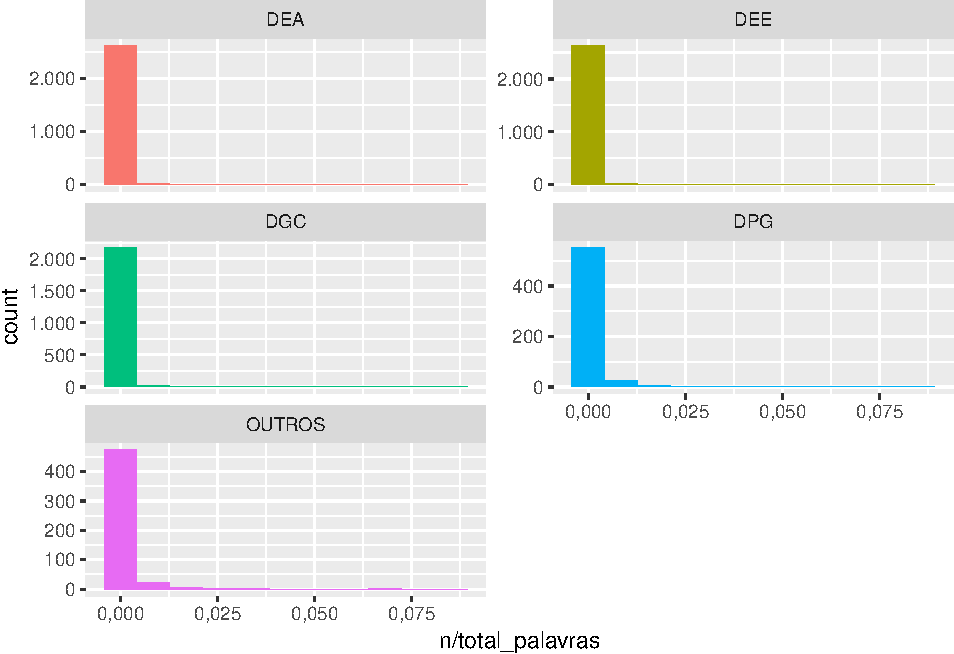
\includegraphics{markdown_v24_files/figure-latex/unnamed-chunk-25-1.pdf}

\begin{itemize}
\tightlist
\item
  Palavras mais frequentes por diretoria
\end{itemize}

\begin{Shaded}
\begin{Highlighting}[]
\NormalTok{PROP_PALAVRA =}\StringTok{ }\NormalTok{diretoria_palavras }\OperatorTok
\StringTok{    }\KeywordTok{mutate}\NormalTok{(}\DataTypeTok{palavra =} \KeywordTok{str_extract}\NormalTok{(palavra, }\StringTok{"[a-z']+"}\NormalTok{)) }\OperatorTok
\StringTok{    }\KeywordTok{count}\NormalTok{(DIRETORIA, palavra) }\OperatorTok
\StringTok{    }\KeywordTok{group_by}\NormalTok{(DIRETORIA) }\OperatorTok
\StringTok{    }\KeywordTok{mutate}\NormalTok{(}\DataTypeTok{proportion =}\NormalTok{ n }\OperatorTok{/}\StringTok{ }\KeywordTok{sum}\NormalTok{(n)) }\OperatorTok
\StringTok{    }\KeywordTok{select}\NormalTok{(}\OperatorTok{-}\NormalTok{n) }\OperatorTok
\StringTok{    }\KeywordTok{spread}\NormalTok{(DIRETORIA, proportion)}
\end{Highlighting}
\end{Shaded}

\begin{itemize}
\tightlist
\item
  Zipf's law
\end{itemize}

\begin{Shaded}
\begin{Highlighting}[]
\NormalTok{freq_by_rank <-}\StringTok{ }\NormalTok{diretoria_palavras }\OperatorTok
\KeywordTok{group_by}\NormalTok{(DIRETORIA) }\OperatorTok
\KeywordTok{mutate}\NormalTok{(}\DataTypeTok{ranque =} \KeywordTok{row_number}\NormalTok{(),}
\StringTok{`}\DataTypeTok{frequência de termos}\StringTok{`}\NormalTok{ =}\StringTok{ }\NormalTok{n}\OperatorTok{/}\NormalTok{total_palavras)}

\CommentTok{# Plot}
\NormalTok{freq_by_rank }\OperatorTok
\KeywordTok{ggplot}\NormalTok{(}\KeywordTok{aes}\NormalTok{(ranque, }\StringTok{`}\DataTypeTok{frequência de termos}\StringTok{`}\NormalTok{, }\DataTypeTok{color =}\NormalTok{ DIRETORIA)) }\OperatorTok{+}
\KeywordTok{geom_abline}\NormalTok{(}\DataTypeTok{intercept =} \OperatorTok{-}\FloatTok{0.62}\NormalTok{, }\DataTypeTok{slope =} \OperatorTok{-}\FloatTok{1.1}\NormalTok{, }\DataTypeTok{color =} \StringTok{"gray50"}\NormalTok{, }\DataTypeTok{linetype =} \DecValTok{2}\NormalTok{) }\OperatorTok{+}
\KeywordTok{geom_line}\NormalTok{(}\DataTypeTok{size =} \FloatTok{1.1}\NormalTok{, }\DataTypeTok{alpha =} \FloatTok{0.8}\NormalTok{, }\DataTypeTok{show.legend =} \OtherTok{TRUE}\NormalTok{) }\OperatorTok{+}
\KeywordTok{scale_x_log10}\NormalTok{(}\DataTypeTok{labels=}\NormalTok{gcomma) }\OperatorTok{+}
\KeywordTok{scale_y_log10}\NormalTok{(}\DataTypeTok{labels=}\NormalTok{gcomma)}
\end{Highlighting}
\end{Shaded}

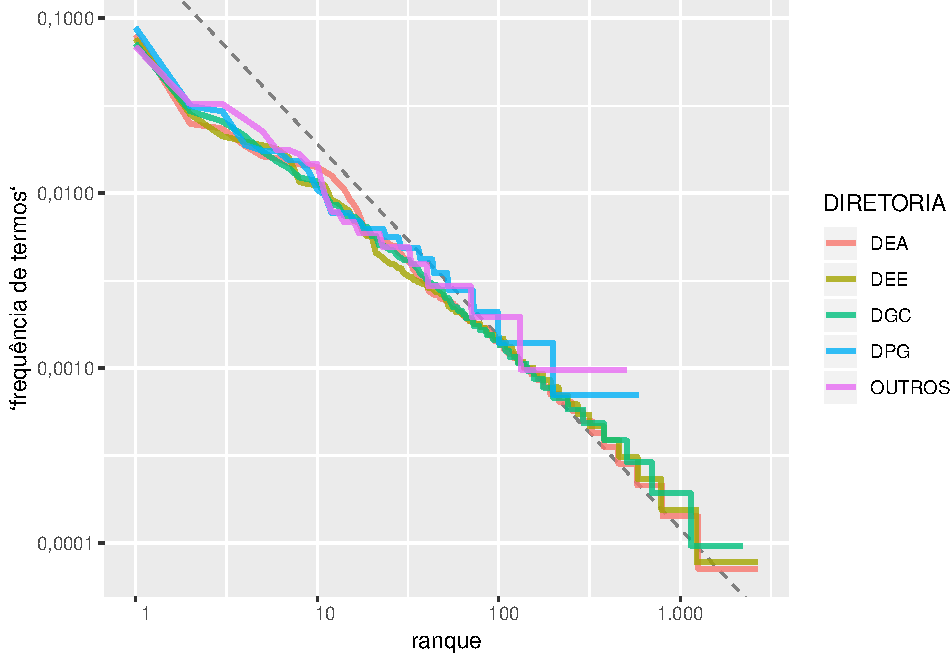
\includegraphics{markdown_v24_files/figure-latex/unnamed-chunk-28-1.pdf}

\paragraph{Frequência de palavras por
diretoria}\label{frequencia-de-palavras-por-diretoria}

\begin{Shaded}
\begin{Highlighting}[]
\NormalTok{diretoria_palavras <-}\StringTok{ }\NormalTok{DB }\OperatorTok
\StringTok{  }\KeywordTok{unnest_tokens}\NormalTok{(palavra, DESCRI_PEDIDO) }\OperatorTok
\StringTok{  }\KeywordTok{count}\NormalTok{(DIRETORIA, palavra, }\DataTypeTok{sort =} \OtherTok{TRUE}\NormalTok{) }\OperatorTok
\StringTok{  }\KeywordTok{ungroup}\NormalTok{()}
\CommentTok{#diretoria_palavras}

\NormalTok{plot_diretoria_palavras <-}\StringTok{ }\NormalTok{diretoria_palavras }\OperatorTok
\StringTok{  }\KeywordTok{bind_tf_idf}\NormalTok{(palavra, DIRETORIA, n) }\OperatorTok
\StringTok{  }\KeywordTok{arrange}\NormalTok{(}\KeywordTok{desc}\NormalTok{(tf_idf)) }\OperatorTok
\StringTok{  }\KeywordTok{mutate}\NormalTok{(}\DataTypeTok{palavra =} \KeywordTok{factor}\NormalTok{(palavra, }\DataTypeTok{levels =} \KeywordTok{rev}\NormalTok{(}\KeywordTok{unique}\NormalTok{(palavra)))) }\OperatorTok
\StringTok{  }\KeywordTok{mutate}\NormalTok{(}\DataTypeTok{DIRETORIA =} \KeywordTok{factor}\NormalTok{(DIRETORIA, }\DataTypeTok{levels =} \KeywordTok{c}\NormalTok{(}\StringTok{"DEA"}\NormalTok{,}
                                                  \StringTok{"DEE"}\NormalTok{,}
                                                  \StringTok{"DGC"}\NormalTok{,}
                                                  \StringTok{"DPG"}\NormalTok{,}
                                                  \StringTok{"OUTROS"}\NormalTok{)))}
\CommentTok{#View(head(plot_diretoria_palavras))}
\CommentTok{#jpeg("02_freq_palavras_dir.jpeg")}
\NormalTok{plot_diretoria_palavras }\OperatorTok
\KeywordTok{group_by}\NormalTok{(DIRETORIA) }\OperatorTok
\KeywordTok{top_n}\NormalTok{(}\DecValTok{10}\NormalTok{, tf_idf) }\OperatorTok
\KeywordTok{ungroup}\NormalTok{() }\OperatorTok
\KeywordTok{mutate}\NormalTok{(}\DataTypeTok{palavra =} \KeywordTok{reorder}\NormalTok{(palavra, tf_idf)) }\OperatorTok
\KeywordTok{ggplot}\NormalTok{(}\KeywordTok{aes}\NormalTok{(palavra, tf_idf, }\DataTypeTok{fill =}\NormalTok{ DIRETORIA)) }\OperatorTok{+}
\KeywordTok{geom_col}\NormalTok{(}\DataTypeTok{show.legend =} \OtherTok{FALSE}\NormalTok{) }\OperatorTok{+}
\KeywordTok{labs}\NormalTok{(}\DataTypeTok{x =} \OtherTok{NULL}\NormalTok{, }\DataTypeTok{y =} \StringTok{"tf-idf"}\NormalTok{) }\OperatorTok{+}
\KeywordTok{facet_wrap}\NormalTok{(}\OperatorTok{~}\NormalTok{DIRETORIA, }\DataTypeTok{ncol =} \DecValTok{2}\NormalTok{, }\DataTypeTok{scales =} \StringTok{"free"}\NormalTok{) }\OperatorTok{+}
\KeywordTok{coord_flip}\NormalTok{() }\OperatorTok{+}\StringTok{ }
\KeywordTok{scale_y_continuous}\NormalTok{(}\DataTypeTok{labels=}\NormalTok{gcomma)}
\end{Highlighting}
\end{Shaded}

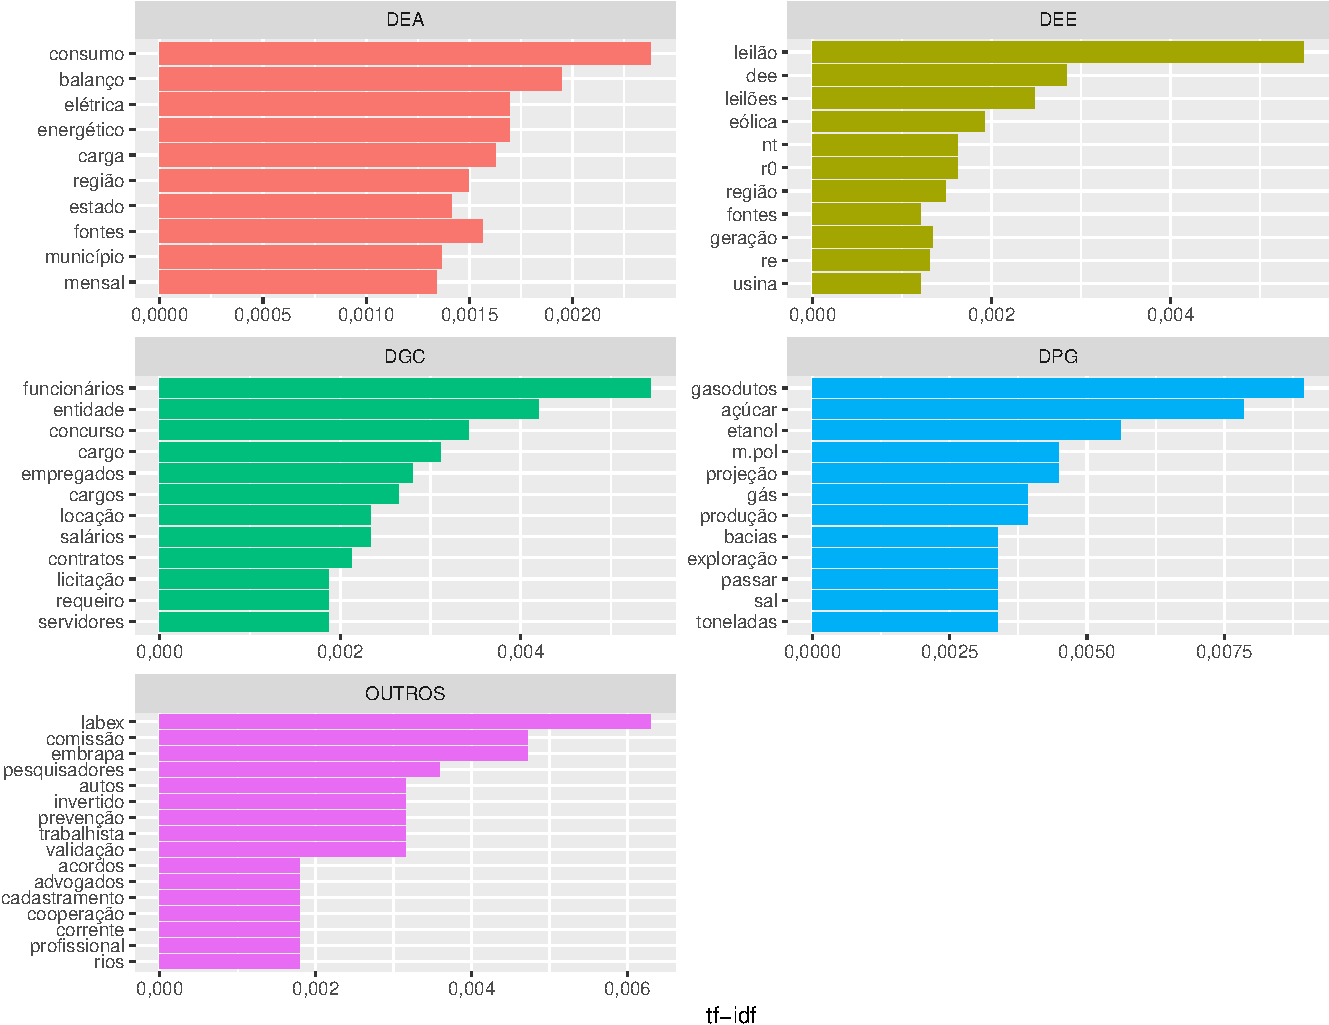
\includegraphics{markdown_v24_files/figure-latex/02_freq_palavras_dir-1.pdf}

\begin{Shaded}
\begin{Highlighting}[]
\CommentTok{#dev.off()}
\end{Highlighting}
\end{Shaded}

\paragraph{Filtrando um pedaço de
texto}\label{filtrando-um-pedaco-de-texto}

\begin{Shaded}
\begin{Highlighting}[]
\NormalTok{DB }\OperatorTok
\KeywordTok{filter}\NormalTok{(}\KeywordTok{str_detect}\NormalTok{(DESCRI_PEDIDO, }\StringTok{"r0"}\NormalTok{)) }\OperatorTok
\KeywordTok{select}\NormalTok{(DESCRI_PEDIDO) }\OperatorTok
\StringTok{  }\KeywordTok{head}\NormalTok{()}
\end{Highlighting}
\end{Shaded}

\begin{verbatim}
##                                                                                                                                                                                                                                                                                                                                                                                                                                                                                                                                                 DESCRI_PEDIDO
## 1                                                                                                                                                                                                                                                                          Prezados,\n\nSolicitamos que o deck do Newave 22.6 utilizado para Revisão da Garantia Física de UHEs, conforme consta da Nota Técnica EPE-DEE-RE-097/2016-r0 da Empresa de Pesquisa Energética -  EPE, nos seja enviado para conhecimento, por gentileza.\n\nObrigada,\nGraziella.
## 2                                                                                                                                                                                                                                                                                                                                                                                                                                                        Gostaria de ter acesso à Nota Técnica EPE-DEE-RE-097/2016-r0, pois não a encontro disponível online.
## 3 Solicitamos para nossa análise cópias dos relatórios nºs EPE-DEE-RE-147/2008-r0 que trata dos ESTUDOS RELATIVOS AOS GRANDES APROVEITAMENTOS HIDRELÉTRICOS NA REGIÃO AMAZÔNICA – Análise do sistema de atendimento aos estados do Acre e Rondônia no período Pré-Madeira – dezembro de 2008 e do relatório nº RE-EPES–4.010/08, que trata do SISTEMA ACRE-RONDÔNIA R2 – Estudos de Transitórios Eletromagnéticos e Condutor Econômico das LTs 230 kV P.Velho – Abunã – Rio Branco – janeiro de 2009.\n\nAgradecemos breve retorno.\n\nAtt.\n\nMônica\n\n\n\n
## 4                                                                                                                                                                                                                                                                                                                                                                            Cópia do documento EPE-DEE-RE-083/2010-r0, “Estudo de Integração das Usinas Hidrelétricas Previstas para o Estado de Santa Catarina”, elaborado pela EPE em novembro de 2010. \n
## 5                                                                                                                                                                                                                                                                                                                                                                                                                                                                                                       Solicito cópia da Nota Técnica EPE-DEE-RE-097/2016-r0
## 6                                                                                                                                                                                                                                                                                                                                                                                                          Bom dia, por gentileza gostaria ter acesso ao parecer técnico EPE-DEE-PT-051/2016-r0 e projeto alternativo apresentado pela tecnogera.\n\nObrigada
\end{verbatim}

Uma limpeza removendo palavras sem significado semântico
(\textbf{stopwords}) pode auxiliar o algoritmo a retornar palavras ainda
mais acertivas

\subsubsection{Stemming}\label{stemming}

Podemos diminuir redundâncias por parte do algoritmo ensinando-o a
compreender palavras que podem estar escritas de forma diferente mas que
em significado semântico são semelhantes. Para isso, analisamos o
radical de palavras com um mesmo prefixo mas com sufixos diferentes seja
por quisistos como gênero ou plural.

Exemplos:

leilão \(\propto\) leilões estado \(\propto\) estados região \(\propto\)
regiões

\texttt{Falta\ implementar}

Usando o pacote \texttt{ptstem}

\begin{Shaded}
\begin{Highlighting}[]
\KeywordTok{library}\NormalTok{(ptstem)}
\KeywordTok{ptstem}\NormalTok{(DB}\OperatorTok{$}\NormalTok{DESCRI_PEDIDO[}\DecValTok{227}\NormalTok{])}
\end{Highlighting}
\end{Shaded}

\begin{verbatim}
## [1] "Sou funcionário da Simple Energy, empresa representante da UTE Manauara. Estou realizando um levantamento sobre o cadastro dessa usina nos órgãos competentes (Aneel/CCEE/ONS/EPE, etc). E, gostaria de receber a Nota Técnica que subsidiou a publicação da garantia física da usina, publicação pela Portaria MME nº 185, de 28 de dezembro de 2012."
\end{verbatim}

\begin{Shaded}
\begin{Highlighting}[]
\NormalTok{stemming1 =}\StringTok{ }\KeywordTok{ptstem}\NormalTok{(DB}\OperatorTok{$}\NormalTok{DESCRI_PEDIDO)}
\CommentTok{#ptstem(diretoria_palavras$palavra)}
\end{Highlighting}
\end{Shaded}

\paragraph{Frequência de palavras por
diretoria}\label{frequencia-de-palavras-por-diretoria-1}

\begin{Shaded}
\begin{Highlighting}[]
\NormalTok{diretoria_palavras_stem1 <-}\StringTok{ }\NormalTok{DB }\OperatorTok
\StringTok{  }\KeywordTok{mutate}\NormalTok{(}\DataTypeTok{DESCRI_PEDIDO =}\NormalTok{ stemming1) }\OperatorTok
\StringTok{  }\KeywordTok{unnest_tokens}\NormalTok{(palavra, DESCRI_PEDIDO) }\OperatorTok
\StringTok{  }\KeywordTok{count}\NormalTok{(palavra, }\DataTypeTok{sort =} \OtherTok{TRUE}\NormalTok{) }\OperatorTok
\StringTok{  }\KeywordTok{ungroup}\NormalTok{()}
\end{Highlighting}
\end{Shaded}

\begin{Shaded}
\begin{Highlighting}[]
\KeywordTok{cat}\NormalTok{(}\KeywordTok{paste0}\NormalTok{(}\StringTok{"Utilizando o algoritmo de stemming do pacote 'ptstem' o número de palavras chaves sem stemming reduziu de "}\NormalTok{, }\KeywordTok{dim}\NormalTok{(diretoria_palavras)[}\DecValTok{1}\NormalTok{], }\StringTok{" para "}\NormalTok{, }\KeywordTok{dim}\NormalTok{(diretoria_palavras_stem1)[}\DecValTok{1}\NormalTok{], }\StringTok{", após stemming. Uma redução de "}\NormalTok{, }\KeywordTok{round}\NormalTok{(}\DecValTok{100}\OperatorTok{-}\KeywordTok{dim}\NormalTok{(diretoria_palavras_stem1)[}\DecValTok{1}\NormalTok{]}\OperatorTok{*}\DecValTok{100}\OperatorTok{/}\KeywordTok{dim}\NormalTok{(diretoria_palavras)[}\DecValTok{1}\NormalTok{],}\DecValTok{0}\NormalTok{),}\StringTok{"%."}\NormalTok{))}
\end{Highlighting}
\end{Shaded}

\begin{verbatim}
## Utilizando o algoritmo de stemming do pacote 'ptstem' o número de palavras chaves sem stemming reduziu de 8629 para 3879, após stemming. Uma redução de 55%.
\end{verbatim}

Usando o pacote \texttt{rslp}

\begin{Shaded}
\begin{Highlighting}[]
\KeywordTok{library}\NormalTok{(rslp)}
\KeywordTok{rslp}\NormalTok{(DB}\OperatorTok{$}\NormalTok{DESCRI_PEDIDO[}\DecValTok{227}\NormalTok{])}
\end{Highlighting}
\end{Shaded}

\begin{verbatim}
## [1] "Sou funcionario da Simple Energy, empresa representante da UTE Manauara. Estou realizando um levantamento sobre o cadastro dessa usina nos orgaos competentes (Aneel/CCEE/ONS/EPE, etc). E, gostaria de receber a Nota Tecnica que subsidiou a publicacao da garantia fisica da usina, publicada pela Portaria MME nº 185, de 28 de dezembro de 2012."
\end{verbatim}

\begin{Shaded}
\begin{Highlighting}[]
\NormalTok{stemming2 =}\StringTok{ }\KeywordTok{rslp}\NormalTok{(DB}\OperatorTok{$}\NormalTok{DESCRI_PEDIDO)}
\end{Highlighting}
\end{Shaded}

\paragraph{Frequência de palavras por
diretoria}\label{frequencia-de-palavras-por-diretoria-2}

\begin{Shaded}
\begin{Highlighting}[]
\NormalTok{diretoria_palavras_stem2 <-}\StringTok{ }\NormalTok{DB }\OperatorTok
\StringTok{  }\KeywordTok{mutate}\NormalTok{(}\DataTypeTok{DESCRI_PEDIDO =}\NormalTok{ stemming2) }\OperatorTok
\StringTok{  }\KeywordTok{unnest_tokens}\NormalTok{(palavra, DESCRI_PEDIDO) }\OperatorTok
\StringTok{  }\KeywordTok{count}\NormalTok{(palavra, }\DataTypeTok{sort =} \OtherTok{TRUE}\NormalTok{) }\OperatorTok
\StringTok{  }\KeywordTok{ungroup}\NormalTok{()}
\end{Highlighting}
\end{Shaded}

\begin{Shaded}
\begin{Highlighting}[]
\KeywordTok{cat}\NormalTok{(}\KeywordTok{paste0}\NormalTok{(}\StringTok{"Utilizando o algoritmo de stemming do pacote 'rslp' o número de palavras chaves sem stemming reduziu de "}\NormalTok{, }\KeywordTok{dim}\NormalTok{(diretoria_palavras)[}\DecValTok{1}\NormalTok{], }\StringTok{" para "}\NormalTok{, }\KeywordTok{dim}\NormalTok{(diretoria_palavras_stem2)[}\DecValTok{1}\NormalTok{], }\StringTok{", após stemming. Uma redução de "}\NormalTok{, }\KeywordTok{round}\NormalTok{(}\DecValTok{100}\OperatorTok{-}\KeywordTok{dim}\NormalTok{(diretoria_palavras_stem2)[}\DecValTok{1}\NormalTok{]}\OperatorTok{*}\DecValTok{100}\OperatorTok{/}\KeywordTok{dim}\NormalTok{(diretoria_palavras)[}\DecValTok{1}\NormalTok{],}\DecValTok{0}\NormalTok{),}\StringTok{"%."}\NormalTok{))}
\end{Highlighting}
\end{Shaded}

\begin{verbatim}
## Utilizando o algoritmo de stemming do pacote 'rslp' o número de palavras chaves sem stemming reduziu de 8629 para 5376, após stemming. Uma redução de 38%.
\end{verbatim}

Uma redução considerável no número de termos ocorreu ao usar o algoritmo
\texttt{ptstem}, cerca de 55\% de redução de termos versus 38\%
utilziando o algoritmo \texttt{rslp}.

Vale ressaltar, tabmbém, o tempo de processamento que ambos os
algoritmos requerem.

\begin{Shaded}
\begin{Highlighting}[]
\NormalTok{temp_stem1 =}\StringTok{ }\KeywordTok{proc.time}\NormalTok{()}
\KeywordTok{ptstem}\NormalTok{(DB}\OperatorTok{$}\NormalTok{DESCRI_PEDIDO)}
\end{Highlighting}
\end{Shaded}

\begin{verbatim}
##   [1] "\nA Empresa de Pesquisa Energética (vinculada ao Ministério de Minas e Energias) indica em seu site que o diretor e presidente desta empresa pública, dependente do tesouro nacional, recebem os salários abaixo citados.\n\nDiretor da Empresa de Pesquisa Energética\n32.482,13\n\nPresidente da Empresa de Pesquisa Energética\n33.763,00\n\nTais salários são maiores do que o do presidente da reública e do que os ministros de estado.\nQuestiono se o Ministério autorizou tais salários. \n"                                                                                                                                                                                                                                                                                                                                                                                                                                                                                                                                                                                                                                                                                                                                                                                                                                                                                                                                                                                                                                                                                                                                                                                                                                                                                                                                                                                                                                                                                                                                                                        
##   [2] "Demanda ou carga Energética total (comercial, industrial, residencial e outras ) mensal entre os anos de 1990 a 2017, incluindo regiões, união e estado, para fins de pesquisa acadêmica de mestrado em previsão de series temporais com uso de técnicas de inteligência computacional com redes neurais."                                                                                                                                                                                                                                                                                                                                                                                                                                                                                                                                                                                                                                                                                                                                                                                                                                                                                                                                                                                                                                                                                                                                                                                                                                                                                                                                                                                                                                                                                                                                                                                                                                                                                                                                                                   
##   [3] "Para o setor de economia e mercado de energias da EPE.\nPrezados, sou estudante de doutorado da UFBA e estado precisando de alguns dados referentes aos custos para a produção de energias no Brasil. os dados que precisando são:\n1) quanto se gastou em reais pela produção de energias termelétrica no pais nos últimos 10 anos? Se possível fazer uma divisão por cada anos. De 2007 a 2017.\n2) quanto foi a produção e o consumo de energias hidrelétrica em kwh durante os últimos 10 anos?\n3)quanto foi o aumentos da conta de energias elétrica pela ineficiência das hidrelétrica nos últimos anos, em decorrência da crise hídrica?\n\nNao consegui encontrar esses dados no site. \n\nobrigado\n\nAtt.,\n\nMatteo Nigro"                                                                                                                                                                                                                                                                                                                                                                                                                                                                                                                                                                                                                                                                                                                                                                                                                                                                                                                                                                                                                                                                                                                                                                                                                                                                                                                                       
##   [4] "Prezados, Não localizei no site da EPE o relatório EPE-DEE-RE-008/2016-rev.O- \"Estudo de Atendimento à Região de Campos\", de abril de 2016. Seria possível recebem-lo por e-mail?"                                                                                                                                                                                                                                                                                                                                                                                                                                                                                                                                                                                                                                                                                                                                                                                                                                                                                                                                                                                                                                                                                                                                                                                                                                                                                                                                                                                                                                                                                                                                                                                                                                                                                                                                                                                                                                                                                         
##   [5] "Boa tarde,\n\nMe chamo Felipe e sou aluno do programa de pós-graduação em Economia na Universidade Federal do Ceará.\nEm minha pesquisa, estado necessitando de informações sobre consumo de energias (Comercial e Indústrial) por Unidade\nda Federação. Vi que no banco de dados fornecidos por vocês (nos relatório da EPE) as informações vão de 2006 à 2016.\nVocês poderiam me auxiliar para que eu consiga obter as informações para o período que vai de 1980 à 2004?\n\nIsto é, precisando de informações sobre o consumo de energias, em GWh, comercial e industrial para cada uma das unidade \nda federal no período que se inicia em 1980 e termina em 2004. Este período nao estado disponível no site da EPE.\n\nMelhores Saudações.\n\nFelipe de Sousa Bastos\nDoutorando em Economia\nUFC/Caen"                                                                                                                                                                                                                                                                                                                                                                                                                                                                                                                                                                                                                                                                                                                                                                                                                                                                                                                                                                                                                                                                                                                                                                                                                                                             
##   [6] "Plano Decenal de Expansão de Energia do anos corrente (2018). Adicionalmente, gentileza fornecidos qualquer pública da EPE quem contenha as previsão mais atualizadas sobre os cenários futuros da oferta de derivados de petróleo no Brasil. \n"                                                                                                                                                                                                                                                                                                                                                                                                                                                                                                                                                                                                                                                                                                                                                                                                                                                                                                                                                                                                                                                                                                                                                                                                                                                                                                                                                                                                                                                                                                                                                                                                                                                                                                                                                                                                                            
##   [7] "Solicitamos a obtenção da manifestação do Ministério da Saúde no processo de licenciamento ambiental SEMA MT número n 346973/2012 relativo à UHE Castanheira. Caso estado órgão da administração federal nao tenha se manifestação no referentes processo, favor informações."                                                                                                                                                                                                                                                                                                                                                                                                                                                                                                                                                                                                                                                                                                                                                                                                                                                                                                                                                                                                                                                                                                                                                                                                                                                                                                                                                                                                                                                                                                                                                                                                                                                                                                                                                                                               
##   [8] "\n\nReportagem TV PUC-Rio\nCarol Brizon   06/07/2015  \nPara: imprensa@light.com.br\n\nPrezados,\n\nSou reportagem da TV PUC-Rio e estado entre em contato, pois estado produzindo uma reportagem sobre economia de energias. Assim, gostaria de solicitar os seguintes dados:\n\n- Quanto os brasil gastou com a conta de luz no primeiro semestre do anos passado? E no primeiro semestre desta anos?\n\n- Qual a quanto de energias utilizada pela brasil no primeiro semestre do anos passado? E no primeiro semestre desta anos?\n\n- Quanto o consumo brasil pagava pela energias, em média, no anos passado? Como era a composição da tarifa de energias elétrica? \n\nLembrando que somos do Núcleo de TV do Projeto Comunicar/ PUC-Rio, que\nproduzindo cinco programa para o Canal Universitário do Rio de Janeiro (UTV-\nCanal 11 NET), pela Canal Universitário de São Paulo (CNU) e pela\nPortal PUC-Rio Digital. A TV-PUC é uma instituição sema fins lucrativos e\ntoda a nossa programa tem caráter exclusivamente cultural e educativo.\n\nAguardo retorno.\n\nAtenciosamente,\n\n\nCaroline Brizon\nRepórter TV PUC-Rio\n(21) 3527-1143 – ramal: 2260\n(21) 99874-2901\n\n\nPROJETO COMUNICAR\nVice-Reitoria para Assuntos Comunitários\nRua Marquês de São Vicente, 225/401K - Gávea - 22543-900\nRio de Janeiro - RJ - Tel./fax (021) 3527-1140/ 3527-1143"                                                                                                                                                                                                                                                                                                                                                                                                                                                                                                                                                                                                                                                                                              
##   [9] "Gostaria de saber se e quem estado disponível a íntegra do Plano de Investimento em Energia Elétrica (lançado em 11.08.2015 pela Governo Federal), conta as informações detalhadas sobre o referentes plano, para além das informações sumarizadas na apresentação de slides já disponibilizada na internet, e com posso obter-la."                                                                                                                                                                                                                                                                                                                                                                                                                                                                                                                                                                                                                                                                                                                                                                                                                                                                                                                                                                                                                                                                                                                                                                                                                                                                                                                                                                                                                                                                                                                                                                                                                                                                                                                                          
##  [10] "Gostaria de solicitar o boletim mensal de energias mais recente que vocês tem, pois no site só encontrar o boletim de junho.\nTambém gostaria de um mapa com toda as usinas hidrelétrica do Brasil - em construção, construídas, licitadas e planejadas. Também gostaria de acessar informações sobre o fornecidos de energias que cada uma deveria fornecidos, quanto elas estado fornecidos na reais e porque nao estado fornecidos o que estado previsto.\nAtenciosamente,\nCarol Barão"                                                                                                                                                                                                                                                                                                                                                                                                                                                                                                                                                                                                                                                                                                                                                                                                                                                                                                                                                                                                                                                                                                                                                                                                                                                                                                                                                                                                                                                                                                                                                                                  
##  [11] "Estou trabalhando em um projeto de pesquisa junto ao meu orientador de mestrado na Universidade de São Paulo (USP-RP), e precisando, se possível, de dados de consumo de energias elétrica (total, residencial e da industrial e serviços) para cada município brasil, em periodicidade mensal, desde 2000. Já encontrar em site com a ANEEL por exemplo, estado dados, mas em nível mais agregado (regiões geográficas). Seria possível obter para o nível de município?\n\nObrigado,\nAndre"                                                                                                                                                                                                                                                                                                                                                                                                                                                                                                                                                                                                                                                                                                                                                                                                                                                                                                                                                                                                                                                                                                                                                                                                                                                                                                                                                                                                                                                                                                                                                                               
##  [12] "Estou confeccionando um modelo matemático para calcular a demanda de energias elétrica para os próximos 10 anos. A demanda total do país en encontrar no ONS. Mas estado precisando saber a demanda de energias elétrica em unidade de potência da industrial brasil.\n\nDesde já, muito obrigado!"                                                                                                                                                                                                                                                                                                                                                                                                                                                                                                                                                                                                                                                                                                                                                                                                                                                                                                                                                                                                                                                                                                                                                                                                                                                                                                                                                                                                                                                                                                                                                                                                                                                                                                                                                                          
##  [13] "Prezados, b.a tarde!\n\nSirvo-me do presente para solicitar o COP/CEC da Suape II, referentes ao Leilão 01/2007."                                                                                                                                                                                                                                                                                                                                                                                                                                                                                                                                                                                                                                                                                                                                                                                                                                                                                                                                                                                                                                                                                                                                                                                                                                                                                                                                                                                                                                                                                                                                                                                                                                                                                                                                                                                                                                                                                                                                                            
##  [14] "Prezados,\n\nDesenvolvo um mestrado em economia e energias. Minha dissertação é sobre o sistema elétrica brasil e, por isso, precisando descrevê-lo corretamente.\nPara tanto, gostaria de ter acessar aos dados utilizada para elaborar as figuras 1 e 2 da Nota Tecnica DEA 01/15, Série Recursos Energéticos da Empresa de Pesquisa Energética (EPE) que dizem respeito á:\n\nEvolução da Curva de Carga diária no SIN no veraão e no inverno, de 2000 a 2014.\n\nEsses dados são originalmente gerados pela Operador NAcional do Sistema (ONS), mas a EPE certamente os tem em planilha, jaá que foram utilizada para elaborar os referentes gráficos da Nota Técnica DEA 01/2015.\n\nSe puder recebem esses dados no formato de planilha excel, agradeço imensamente.\n\nMuito obrigado."                                                                                                                                                                                                                                                                                                                                                                                                                                                                                                                                                                                                                                                                                                                                                                                                                                                                                                                                                                                                                                                                                                                                                                                                                                                                               
##  [15] "Prezados,\n\nDesenvolvo meu mestrado em economia energética e precisando descrevê o sistema elétrica nacinal em minha dissertação. Por nao ter consegui encontrar tais informações nas pública oficiais, venho pedi-las a vocês.\nGostaria de recebem informações sobre: a 0rdem de despacho de fonte (hidrelétrica, biomassa, gás natural, etc) de gerados de energias elétrica para atendimento às demanda de base, intermediária e de pico diário.\nMais especificamente:\n1 - Quais as fonte que são regular e diariamente despacho para atendimento a demanda de base do SIN e quanto dessa demanda cada uma dessa fonte atendimento, em GW/h?\n2 - Quais as fonte que são regular e diariamente despacho para atendimento a demanda intermediária do SIN e quanto dessa demanda cada uma dessa fonte atendimento, em GW/h?\n3 - Quais as fonte que são regular e diariamente despacho para atendimento a demanda de pico do SIN e quanto dessa demanda cada uma dessa fonte atendimento, em GW/h?\n4 - Qual é a divisão em termos da demanda total do SIN, entre as demanda básica, intermediária e de pico? Quais seu perfis de carga ao longo do d.a (básica dados de curva de carga diária classificados em demanda básica, intermediária e de pico)?\n\nEsses dados, acredito, são gerados pela Operador Nacional do Sistema (ONS), e possivelmente estado também em posso da Empresa de Pesquisa Energética (EPE).\n\nObrigado.\n"                                                                                                                                                                                                                                                                                                                                                                                                                                                                                                                                                                                                                                
##  [16] "Prezados, b.a tarde!\n\nGostaria, por gentileza, saber se possuem também dados sobre o consumo do óleo combustível por Estado (UF) e nao somente a quanto vendida (\"Vendas, pela Distribuidoras, dos Derivados Combustíveis de Petróleo (barris equivalentes de petróleo\") \n\nUtilizo estado informações para fazer um estudante de trabalhando de conclusão de curso e percebi que a quanto vendida nao é necessariamente a quanto consumo. \n\nAguardo retorno, obrigado!\n\nAtt, Felipe."                                                                                                                                                                                                                                                                                                                                                                                                                                                                                                                                                                                                                                                                                                                                                                                                                                                                                                                                                                                                                                                                                                                                                                                                                                                                                                                                                                                                                                                                                                                                                                              
##  [17] "Prezadxs,\n\nSolicito dados referentes ao consumo de energias elétrica dos prédios pública. Os dados poderiam seria discriminados pela instâncias administração (federal, estadual e municipal) ou agregado, caso nao posso ocorrer a discriminados. Caso esses dados puder seria separados pela entidades federal iria seria de grande ajuda. \nSe vocês possuírem alguns base histórica disponível, referentes ao consumo dos prédios pública, a partir dos anos 2000 (ou data disponível), também gostaria de obter-la. Caso isso nao foram possível, gostaria de ter os dados mais recente dessa consumo.\nAtenciosamente,\nGabriel\n"                                                                                                                                                                                                                                                                                                                                                                                                                                                                                                                                                                                                                                                                                                                                                                                                                                                                                                                                                                                                                                                                                                                                                                                                                                                                                                                                                                                                                                   
##  [18] "Gostaria de uma pesquisa/estudante se disponível a respeito da previsão de crescimento do setor elétrica nacional no período de 2016 a 2020; assim com também a previsão de investimento no setor.\nTambém se disponível ou de alguns maneira possível, gostaria da previsão/demanda para equipamentos de network (switches, roteadores, firewalls, conversores de mídia e meio físico) para estado mesmo período no setor elétrica, para os novos empreendimentos assim com também para  o retrofit no parque tecnológico atualizadas.\n\n"                                                                                                                                                                                                                                                                                                                                                                                                                                                                                                                                                                                                                                                                                                                                                                                                                                                                                                                                                                                                                                                                                                                                                                                                                                                                                                                                                                                                                                                                                                                                 
##  [19] "Gostaria de informações sobre o Programa de Pesquisa e Desenvolvimento (P&D) do Setor de Energia Elétrica. Ele estabelece que concessionárias e permissionárias de distribuidoras, gerados e transmissão de energias elétrica apliquem anualmente partir da s.a receita operacional líquida nas ações desta programa, sendo que cerca de 13% dos recursos são direcionados ao MME anualmente.\nGostaria das seguintes informações para o período de 2010 a 2015:\n\n1) Em qual ações são investimento os recursos direcionados ao MME proveniente do Programa de P&D do Setor de Energia Elétrica? São necessariamente ações de P&D voltadas ao setor elétrica? \n2) Qual o nome de cada programa e o volume dos recursos aplicados respectivamente?\n\nObrigada!\n"                                                                                                                                                                                                                                                                                                                                                                                                                                                                                                                                                                                                                                                                                                                                                                                                                                                                                                                                                                                                                                                                                                                                                                                                                                                                                                         
##  [20] "Solicitação de dados de incentivos fiscais para empresa produtoras de energias na federal. \n\nGostaria de dados desde a Lei do Petróleo em 1997 a respeito de quanto empresa recebem incentivos e qual valor, dividido por quanto por cento são para energias renováveis e nao-renováveis. \nSe possível, no período entre 1998 e 2015.\n\nO intuito é veraão a evolução dos incentivos fiscais para energias renováveis."                                                                                                                                                                                                                                                                                                                                                                                                                                                                                                                                                                                                                                                                                                                                                                                                                                                                                                                                                                                                                                                                                                                                                                                                                                                                                                                                                                                                                                                                                                                                                                                                                                                  
##  [21] "Projeção % de aumentos para os combustível em 2016 (gasolina, etanol, diesel, óleo combustivel, glp)"                                                                                                                                                                                                                                                                                                                                                                                                                                                                                                                                                                                                                                                                                                                                                                                                                                                                                                                                                                                                                                                                                                                                                                                                                                                                                                                                                                                                                                                                                                                                                                                                                                                                                                                                                                                                                                                                                                                                                                        
##  [22] "Prezados, estado fazer um trabalhando e precisando saber a originalmente do valor novos de reposição, mas até o momento nao consegui encontrar nada referentes a esses método. Solicito o material que mostra a originalmente do VNR, por favor. Obrigada."                                                                                                                                                                                                                                                                                                                                                                                                                                                                                                                                                                                                                                                                                                                                                                                                                                                                                                                                                                                                                                                                                                                                                                                                                                                                                                                                                                                                                                                                                                                                                                                                                                                                                                                                                                                                                  
##  [23] "Prezados,\n\nSolicitamos que o deck do Newave 22.6 utilizada para Revisão da Garantia Física de UHEs, conforme consta da Nota Técnica EPE-DEE-RE-097/2016-r0 da Empresa de Pesquisa Energética -  EPE, nos seja enviado para conhecimento, por gentileza.\n\nObrigada,\nGraziella."                                                                                                                                                                                                                                                                                                                                                                                                                                                                                                                                                                                                                                                                                                                                                                                                                                                                                                                                                                                                                                                                                                                                                                                                                                                                                                                                                                                                                                                                                                                                                                                                                                                                                                                                                                                          
##  [24] "Boa tarde!\n\nEstou estudante a viabilidade de implementar um sistema de uma micro usinas solar e gostaria de alguns dados para embasar esses estudante.\nMoro em Paracatu, MG  que pertence a mesorregião Noroeste de Minas. Gostaria de saber se o MME possuem alguns estudante ou alguns informações sobre a incidência dos meses com maiores concentração de raios solar, horários ou até mesmo incidência da chuva na regiões.\n\nTambém gostaria de saber se possuem alguns material sobre energias renováveis, em particular, energias solar que posso seria compartilhado. \n\nSeria de muito bom proveito esses informações, uma vez que a implementar de um sistema renováveis de energias vem muito a calhar em tempos de escassez dos recursos hídrica, bem com aos custos da energias hidrelétrica. \n\nAtenciosamente, "                                                                                                                                                                                                                                                                                                                                                                                                                                                                                                                                                                                                                                                                                                                                                                                                                                                                                                                                                                                                                                                                                                                                                                                                                                       
##  [25] "Para realizar minha Monografia gostaria de ter acessar sobre os dados da evolução da oferta de energias elétrica originada a partir do bagaço da cana de açúcar. Se possível, enviado dados de, pela menos, 10 anos. E, caso seja possível, colocar também dados para outras produtoras derivados da cana, com melaço e palha. Obrigado."                                                                                                                                                                                                                                                                                                                                                                                                                                                                                                                                                                                                                                                                                                                                                                                                                                                                                                                                                                                                                                                                                                                                                                                                                                                                                                                                                                                                                                                                                                                                                                                                                                                                                                                                    
##  [26] "\nA Empresa de Pesquisa Energética (vinculada ao Ministério de Minas e Energias) indica em seu site que o diretor e presidente desta empresa pública, dependente do tesouro nacional, recebem os salários abaixo citados.\n\nDiretor da Empresa de Pesquisa Energética\n32.482,13\n\nPresidente da Empresa de Pesquisa Energética\n33.763,00\n\nTais salários são maiores do que o do presidente da reública e do que os ministros de estado.\nQuestiono se o Ministério autorizou tais salários. "                                                                                                                                                                                                                                                                                                                                                                                                                                                                                                                                                                                                                                                                                                                                                                                                                                                                                                                                                                                                                                                                                                                                                                                                                                                                                                                                                                                                                                                                                                                                                                          
##  [27] "Prezados,\nConforme Art. 24 do Decreto nº 5163/2004, nos leilão de energias proveniente de empreendimentos existentes, cada agente de distribuidoras poderiam contratar energias elétrica correspondente ao seu montante de reposição e à recuperação de mercado.\nEm seu parágrafo § 1º-A, a recuperação de mercado é definida com o somos do montante de reposição nao contratar nos cinco anos anteriores ao anos de realizar do leilão.\nDado o exposto, solicitamos os valor dos montante de reposição declarados por cada distribuidoras de energias nos leilão de energias elétrica dos últimos 5 anos."                                                                                                                                                                                                                                                                                                                                                                                                                                                                                                                                                                                                                                                                                                                                                                                                                                                                                                                                                                                                                                                                                                                                                                                                                                                                                                                                                                                                                                                              
##  [28] "Solicito os dados coletados referentes aos questiono em anexo."                                                                                                                                                                                                                                                                                                                                                                                                                                                                                                                                                                                                                                                                                                                                                                                                                                                                                                                                                                                                                                                                                                                                                                                                                                                                                                                                                                                                                                                                                                                                                                                                                                                                                                                                                                                                                                                                                                                                                                                                              
##  [29] "Demanda ou carga Energética total (comercial, industrial, residencial e outras ) mensal entre os anos de 1990 a 2017, com a finalidade para estudante de previsão de series temporais em demanda energética mensal entre 1990 a 2017, incluindo regiões, união e estado , utilizada técnicas de inteligência computacional com redes neurais."                                                                                                                                                                                                                                                                                                                                                                                                                                                                                                                                                                                                                                                                                                                                                                                                                                                                                                                                                                                                                                                                                                                                                                                                                                                                                                                                                                                                                                                                                                                                                                                                                                                                                                                               
##  [30] "Gostaria de ter acessar à Nota Técnica EPE-DEE-RE-097/2016-r0, pois nao a encontrar disponível online."                                                                                                                                                                                                                                                                                                                                                                                                                                                                                                                                                                                                                                                                                                                                                                                                                                                                                                                                                                                                                                                                                                                                                                                                                                                                                                                                                                                                                                                                                                                                                                                                                                                                                                                                                                                                                                                                                                                                                                      
##  [31] "Por favor, eu gostaria de solicitar o Relatório-Síntese da Empresa de Pesquisa Energética atualizadas (2017/18). Por exemplo, neste mesmo relatório, em 2013, a participação de fonte renováveis na matriz energética brasil era de 42,4%, significativamente acima da média mundial , calcular em 13,2% pela Agência Internacional de Energia. As fonte nao-renováveis tinham a participação de 57,6%. A  repartição  da  oferta interna   de   energias,   segundo   o   Relatório-Síntese   (EMPRESA   DE   PESQUISA ENERGÉTICA,  2013),  ocorrer  da  seguintes  maneira:  (i)  42,4%  para  as  fonte  de energias renováveis e; (ii) 57,6% para as fonte nao renováveis. Dentre as fonte de energias   renováveis   (42,4%)   o   seguintes   cenários:   (i)   a   biomassa   da   cana   é responsável  pela  maiores  participação  (15,4%);  seguida  pela  energias  hidráulica  e eletricidade  com  13,8%  de  participação. \n\nComo estado em atualizadas? Este é o meu objetivo.\n\nLembrando que, a Empresa de Pesquisa Energética estado vinculada ao Ministério de Minas e Energia (MME).\n\nEste mesmo relatório do anos de 2013 encontrar-se anexo. Estou a procura do anos de 2017 ou o mais atualizadas.\n\nReferencia utilizada: \nEPE.  Empresa  de  Pesquisa  Energética. Balanço  energética  nacional  2013,  anos base  2012:  relatório  síntese.  Rio  de  Janeiro:  EPE,  2013.  55 p.  Disponível  em: \n https://ben.e.e.gov.br/downloads/S%C3%ADntese%20do%20Relat%C3%B3rio%20Final_2013_Web.pdf . Acesso em: 28 jun. 2013.\n\n"                                                                                                                                                                                                                                                                                                                                                                                                                                                                                                          
##  [32] "Boa tarde, \n\nGostaria de solicitar os dados histórica de Estatísticas do Consumo de Energia Elétrica (GWh), divulgados pela ONS na Resenha Mensal. \n\nA finalidade é estudante econométrico da series histórica de consumo de energias no Brasil e nos setor da economia. \n\nObrigada. "                                                                                                                                                                                                                                                                                                                                                                                                                                                                                                                                                                                                                                                                                                                                                                                                                                                                                                                                                                                                                                                                                                                                                                                                                                                                                                                                                                                                                                                                                                                                                                                                                                                                                                                                                                                 
##  [33] "Eu João Emanuel Lós Reis Fidalgo, sou partir interessada pela PBTE, Diretor Técnico."                                                                                                                                                                                                                                                                                                                                                                                                                                                                                                                                                                                                                                                                                                                                                                                                                                                                                                                                                                                                                                                                                                                                                                                                                                                                                                                                                                                                                                                                                                                                                                                                                                                                                                                                                                                                                                                                                                                                                                                        
##  [34] "Goiás - \nRio Quente\nFlores de Goiás\nPalmeiras de Goiás\nCristalina\n\nMato-Grosso\nCampinápolis\nCampo Novo do Parecis\nPontes e Lacerda\n\nMato-Grosso do Sul\nCosta Rica\nIvinhema\nNaviraí\n"                                                                                                                                                                                                                                                                                                                                                                                                                                                                                                                                                                                                                                                                                                                                                                                                                                                                                                                                                                                                                                                                                                                                                                                                                                                                                                                                                                                                                                                                                                                                                                                                                                                                                                                                                                                                                                                                          
##  [35] "Nós estado fazer um trabalhando sobre energias núcleo.\n\nGostaria de saber alguns informações, são as seguintes\n\nQual é a porcentagem de utilizada de energias núcleo no brasil?\nQual é a porcentagem de utilizada de energias núcleo no Mundo?\n\nQual é o custos em MWh da energias núcleo no brasil?\nQual é o custos em MWh da energias núcleo no Mundo?\n\nQual é a disponibilizada da energias núcleo no brasil?\nQual é a Disponibilidade da energias núcleo no Mundo?\n\nQual é a participação na matriz da energias núcleo no brasil?\nQual é a participação na matriz da energias núcleo no Mundo?\n\nObrigado desde já.\n\n\n   "                                                                                                                                                                                                                                                                                                                                                                                                                                                                                                                                                                                                                                                                                                                                                                                                                                                                                                                                                                                                                                                                                                                                                                                                                                                                                                                                                                                                                             
##  [36] "Gostaria de solicitar dados de consumo anualmente médio de energias elétrica por município para os anos de 2013, 2014 e 2015."                                                                                                                                                                                                                                                                                                                                                                                                                                                                                                                                                                                                                                                                                                                                                                                                                                                                                                                                                                                                                                                                                                                                                                                                                                                                                                                                                                                                                                                                                                                                                                                                                                                                                                                                                                                                                                                                                                                                               
##  [37] "1 - Solicito que seja informações quanto usinas termoelétricas existentes no Brasil. Quantas estado ativas e quanto estado inativas.\n2 - Solicito que seja informações quanto usinas termoelétricas operador se utilizada de Terminal de Regaseificação.\n3 - Solicito que seja explicitado qual o papel da Eletrobrás no encaminhamento dos processo de licenciamento de Usinas Termoelétricas no Brasil.\n4 - Solicito que seja explicitado se há estudante que enunciem a necessariamente de ampliação da matriz energética do Brasil.\n5 - Solicito que seja explicitado se a ELETROBRÁS participação do processo de licenciamento ambiental das Usinas Termoelétricas do Brasil. \n6 - A utilizada de Terminal Offshore - Terminal de Regaseificação estado presente nas Usinas Termoelétricas Brasileiras?  Em qual Usinas?\n"                                                                                                                                                                                                                                                                                                                                                                                                                                                                                                                                                                                                                                                                                                                                                                                                                                                                                                                                                                                                                                                                                                                                                                                                                                        
##  [38] "A Centrais Elétricas do Norte do Brasil S.A. \n\nCC.: Departamento de Geoprocessamento\n \nCaros, permitam-me acessar o conhecimento desta Instituição. Peço ajuda para:\n \n1-   identificar a melhores informações oficiais sobre geodados (shapefile) de centrais de gerados de energias, reservatórios, linhas de transmissão e outras infraestruturas associadas a gerados e distribuidoras de energias no território correspondente a Amazônia Legal;\n \n2-          Documentos oficiais recente que abordam aspectos da infraestruturas de energias na Amazônia.\n \n\nContextualizarei o pedi a seguida. Sou consultor da empresa Amazônia Socioambiental e atualizadas realizar uma pesquisa coordenada pela Instituto Nacional de Ciência e Tecnologia (INCT) para Mudanças Climáticas.\n \nEsta pesquisa resultará em um conjunto de dados georreferenciados sobre o histórica da infraestruturas na Amazônia Legal para uma compreensão geográficas dos polígonos, linhas e pontes, anos-a-anos.\n \nEstes dados seria posteriormente disponibilizada pela INCT para Mudanças Climáticas em vários formato e de forma irrestrita para acessar pública, e permitam análises íntegra de diversas infraestruturas de transporte, comunicar e energias tornando possível maiores planejadas e redução de impactos negativos dos empreendimentos.\n \n \nAtenciosamente,      Marco Aurélio."                                                                                                                                                                                                                                                                                                                                                                                                                                                                                                                                                                                                                                                                        
##  [39] "Olá, tudo bem?\n\nSou aluno de iniciação científica do laboratório GruMa (grupo de modelo atmosférica de Santa Maria) da Universidade Federal de Santa Maria -UFSM, orientador pela professor Vagner Anabor. Estou fazer uma pesquisa sobre a relação entre a temperatura e demanda de energias elétrica. Para tanto, eu precisando de dados de demanda de energias elétrica para o período de 1998 até 2016 para a cidade de Santa Maria - RS.  Será que vocês poderiam me mandar tais dados?\n\nDesde já eu agradeço\n\nAtt,\nAngélica Lais Gehrke "                                                                                                                                                                                                                                                                                                                                                                                                                                                                                                                                                                                                                                                                                                                                                                                                                                                                                                                                                                                                                                                                                                                                                                                                                                                                                                                                                                                                                                                                                                                       
##  [40] "Solicito os dados refeferente ao consumo mensal de energias elétrica por Unidade Federativa (Estados e Distrito Federal) compreeendendo o período de 1980 a 2017. Informo que localizei o arquivo de Consumo mensal de energias eletricidade por classe, contudo, nao compreende os dados anteriores a 2004, indispensável para o fins desejado. "                                                                                                                                                                                                                                                                                                                                                                                                                                                                                                                                                                                                                                                                                                                                                                                                                                                                                                                                                                                                                                                                                                                                                                                                                                                                                                                                                                                                                                                                                                                                                                                                                                                                                                                           
##  [41] "Caros, sou aluno de doutorado do INPE (Inst. Nacional de Pesquisas Espaciais) e estado à procura de dados de consumo de eletricidade na bacia do rio São Francisco. Busco dados por município ou outras recorte que me permitam análises os principais consumo da bacia. Poderiam fornecidos-lós ou indica alguns funcionário para quem eu posso solicitar?\nAgradeço antecipadamente."                                                                                                                                                                                                                                                                                                                                                                                                                                                                                                                                                                                                                                                                                                                                                                                                                                                                                                                                                                                                                                                                                                                                                                                                                                                                                                                                                                                                                                                                                                                                                                                                                                                                                      
##  [42] "Prezados, \n\nFavor informações:\n1- Qual é a empresa prestadora do serviços de Benefício Farmácia ou Vale Drogaria para: \n\n- entrega de medicamentos (delivery);\n- redes de farmácia credenciadas;\n- reembolso de medicamentos para farmácia nao-credenciadas; \n\n2- Quais foram as empresa prestadora do serviços de Benefício Farmácia ou Vale Drogaria que participação das licitadas pública?\nFavor considerar com referentes os últimos 10 anos.\n\n3- Qual o número do contratar?\n\n4- Qual o número do processo da licitadas?\n\nDesde já, agradeço a atenção prestadora.\n"                                                                                                                                                                                                                                                                                                                                                                                                                                                                                                                                                                                                                                                                                                                                                                                                                                                                                                                                                                                                                                                                                                                                                                                                                                                                                                                                                                                                                                                                                  
##  [43] "Prezados Srs.\nConforme é de vosso conhecimento, o arquivo de Vazões Naturais Afluentes (vazao.dat) utilizada pela NEWAVE em vosso estudante necessitando de um editor para que seu conteúdo seja visualizado.  Ocorre que, diferentemente do ONS que disponibiliza o editor do arquivo de vazões utilizada por e.e, a EPE nao o fazer.\nCom base na lei da transparência, solicitamos a disponibilizada do editor uma vez que é a única forma de se avaliar o seu conteúdo e assim realizar estudante para novos aproveitamentos, checar valor, etc.\nNo aguardo do atendimento da solicitamos, agradeço antecipadamente, \n\nIvana Costa Nasser"                                                                                                                                                                                                                                                                                                                                                                                                                                                                                                                                                                                                                                                                                                                                                                                                                                                                                                                                                                                                                                                                                                                                                                                                                                                                                                                                                                                                                           
##  [44] "Visto a perda de fluxo do Rio em questão, venho solicitar a valiosa colaboração no sentido de obter a series histórica da vazões desta corpo hídrica, se possível desde o iniciação das média até os d.a atualizadas. Esse material seria utilizada com ferramenta de conscientização das autoridades municipal, comunidades em geral e estudante do município.\n- o solicitamos e natural dessa município onde os seu familiares ainda residencial. Como tenha forma acadêmica nessa área tenha interesse em fazer estudante com objetivo de conscientização a população  \n  Desde já agradeço a atenção dispensada\nAtt.\n    Grato Lauro"                                                                                                                                                                                                                                                                                                                                                                                                                                                                                                                                                                                                                                                                                                                                                                                                                                                                                                                                                                                                                                                                                                                                                                                                                                                                                                                                                                                                                                
##  [45] "1) Entre 21/06/1993 e a data desta pedi de informações, esses órgão/entidades, COM PRÉVIA LICITAÇÃO, firmou contratar de locação de imóveis (situados na cidade onde esteja a sede dessa órgão/entidades e/ou no Distrito Federal), na condição de locatário? Caso a resposta a estado questão seja afirmativa, requeiro os número dos editor das licitadas e os número dos respectivos contratar.\n\n2) Entre 21/06/1993 e a data desta pedi de informações, esses órgão/entidades, SEM PRÉVIA LICITAÇÃO (contratar direta), firmou contratar de locação de imóveis, (situados na cidade onde esteja a sede dessa órgão/entidades e/ou no Distrito Federal), na condição de locatário? Caso a resposta a estado questão seja afirmativa, requeiro os número dos contratar e os número dos respectivos processo administração.\n\n3) Esse órgão/entidades é/foi partir locatária, nalgum contratar de locação de imóveis, (situados na cidade onde esteja a sede dessa órgão/entidades e/ou no Distrito Federal),  com vigência entre janeiro/2011 e dezembro/2015? Caso a resposta a estado questão (3) seja afirmativa, requeiro: a) cop dos pareceres jurídicos precedentes às contratar; b) cop dos termos de referentes (projeto básica) e dos respectivos contratar. SE as contratar houverem sido precedentes de licitadas, requeiro também cop dos respectivos editor.\n\n4) Alguns órgão/entidades da Administração Pública Federal, em procedimento que pareceres voltadas à instaurar desestímulo quanto ao uso da Lei 12.527/2011 (e decreto regulamentador), orientador os cidade que requerem informações a realizar pesquisa no Portal da Transparência (e/ou noutras páginas eletrônicas) sema fornecidos elementos suficientes/eficazes (tais com links,  número dos contratar, número dos processo administração etc.) para que as informações requeridas seja encontrar, dentre milhares de outras. Caso seja estado o procedimento adotado nessa órgão/entidades, requeiro o nome e o carga da autoridades que o tenha determinado.\n"                   
##  [46] "Prezados,\n\nA EPE auxiliar o poderiam concedente na definida das indenizações e receita das concessionárias que eram passado de ter seu contratar prorrogados nos termos da MP 579/2012. Um dos documentos editor pela EPE refere-se a uma Nota Técnica que análises uma taxa de lucratividade a seria aplicados a esses contratar prorrogados. Referida Nota Técnica chegou ao número de 10% sobre a receita, conforme notícia abaixo e demais informações no site da ANEEL, que também dão conta de tais documentos. Desta forma, solicitamos o enviado de referentes documentos para conhecimento. Obrigado antecipadamente.\n\n\n\n\nhttps://www.canalenergia.com.br/zpublisher/mato/Retrospectiva.asp?id=93064&a=2012\n\nAgência CanalEnergia - A EPE foi responsável por elaborar uma nota técnicas que sugeriu uma taxa de retorno de 10% para as concessões a seria renováveis, o que nao agradou muito o setor. Como a EPE chegou a esses número?\nMaurício Tolmasquim - Sobre o valor que a Aneel calcular foi adicionada uma margem de lucrativos de 10%. O valor originalmente da Aneel nao tinham a margem de lucrativos. A EPE, na reunião, brigou por isso e considerar que seria necessariamente ter uma margem, porque qualquer prestadora de serviços tem uma lucratividade. A gente aqui fez um trabalhando pegando principais estudante do Tribunal de Contas da União para outras projeto e o valor máximo aceito pela TCU era de 10%. A empresa vai estado sendo remunerada e justamente. Ninguém prestadora um serviços sema remunerada.\nE deveria ficar claro que esses valor da tarifa é só para operador e manter. Qualquer investimento de modernização nao estado incluindo nessa valor. A concessionárias solicitamos autorização da Aneel, que análises o pedi, e seria autorização um aumentos no valor da tarifa para cobrir as modernização que seria feitas. Eu tenha escutado muito dizem que ninguém vai investimento em modernização. Vai sim, porque toda os investimento considerar prudentes seria remunerada na tarifa."          
##  [47] "Sou estudante de mestrado em Economia na Universidade Federal da Bahia (PPGE- UFBA). \nEstou iniciação a dissertação e o tem é \"O Efeito da Densidade Urbana sobre o Consumo de Energia Elétrica na Bahia\" e os os objetivo são:\n- Construir um banco de dados sobre a estrutura das cidade e consumo de energias elétrica por município no estado da Bahia;\n- Analisar as relação factíveis entre economia urbana, economia da energias e economia do meio ambiente. \n- - Estimar os efeito causais da estrutura urbana  sobre a eficiência energética nas cidade da Bahia.\nPara tais trabalhando seria realizar necessitando dos dados de Consumo Energético Residencial Mensal no Estado da Bahia. No site da EPE veriquei a existentes dos dados de consumo energética por regiões e estado. Há possibilidade de disponibilizada tais dados o nível municipal?\n\nGrata pela colaboração!"                                                                                                                                                                                                                                                                                                                                                                                                                                                                                                                                                                                                                                                                                                                                                                                                                                                                                                                                                                                                                                                                                                                                                                         
##  [48] "Olá, sou estudante do doutorado em Economia do PIMES/UFPE e Economista da Companhia Hidro Elétrica do São Francisco (Chesf). Tenho desenvolvo pesquisa na área da Economia da Energia. No momento estado necessitando de dados do setor elétrica brasil. Especificamente: consumo de energias elétrica por município brasil, mensal, por grupo de consumo (residencial, industrial etc). Também necessitando dos preços cobrir pela energias por regiões de atuação das concessionárias. O período para os dados deveria seria toda a series disponível. Desde já agradeço. "                                                                                                                                                                                                                                                                                                                                                                                                                                                                                                                                                                                                                                                                                                                                                                                                                                                                                                                                                                                                                                                                                                                                                                                                                                                                                                                                                                                                                                                                                                
##  [49] "Por gentileza, a Planinvesti Administração e Serviços Ltda., CNPJ n° 029.959.3.2.0.01-46, vem através desta, solicitar a o enviado das informações abaixo, referentes ao seu atualizadas fornecidos Solicitação de Informações contratar de Vale Refeição, Alimentação, Transporte, Combustível e Cultura.\n\nMotivo da solicitamos: Análise do certame para nos precaver e nos preparar para futuros certame.\n\nNome do Órgão: \nTaxa Administrativa:\nEmpresa Vencedora:\nInício e Término do primeiro contratar com o atualizadas fornecidos:\nQuando ocorrer a licitadas (Data/Mês/Ano):\nValor global da licitadas:\nQuantidade de benefício:\nQual modalidade e o n° do certame que foi aberto:\nCaso o contratar seja um termos aditivo, por gentileza, nos informações qual número é:"                                                                                                                                                                                                                                                                                                                                                                                                                                                                                                                                                                                                                                                                                                                                                                                                                                                                                                                                                                                                                                                                                                                                                                                                                                                                              
##  [50] "Prezados, b.a tarde!\n\nSolicito a cop da NT EPE-DEE-RE-077/2008.\n\nEstou realizar alguns estudante pertinentes a CUR e precisando desta arquivo de referentes.\n\nGrato pela atenção!\n\nThiago Paulino\n\n"                                                                                                                                                                                                                                                                                                                                                                                                                                                                                                                                                                                                                                                                                                                                                                                                                                                                                                                                                                                                                                                                                                                                                                                                                                                                                                                                                                                                                                                                                                                                                                                                                                                                                                                                                                                                                                                               
##  [51] "Gostaria iniicalmente de parabenizar a EPE pela ótima Nota Técnica (NT) sobre utilizada de sistema híbridos para o atendimento com energias elétrica de localidades no Acre (Lote III). \n\nA NT apresentação uma solução de suprimento com diesel + solar PV + bateria mais competitiva que opção 100% diesel. Para concluir isto a EPE utilizada um software chamado HOMER. \n\nSeria possível obter cop da base de dados do HOMER desta avaliar?\n\nCordialmente,\nRafael Kelman"                                                                                                                                                                                                                                                                                                                                                                                                                                                                                                                                                                                                                                                                                                                                                                                                                                                                                                                                                                                                                                                                                                                                                                                                                                                                                                                                                                                                                                                                                                                                                                                         
##  [52] "Ola pessoa responsavel,\nUm meu amigo , comerciante , turco da Turquia, quem investimento no Brasil\nEle quem abrir uma fabrica de energias solar e vento para fabricar / produzindo energias elétrica.\nGostaria de saber qual regioes do brasil é melhores para isso .\nQuais lugares o governo dá apoio e qual regioes melhores para estado investimento ?\nObrigado"                                                                                                                                                                                                                                                                                                                                                                                                                                                                                                                                                                                                                                                                                                                                                                                                                                                                                                                                                                                                                                                                                                                                                                                                                                                                                                                                                                                                                                                                                                                                                                                                                                                                                                     
##  [53] "Solicito as memórias de calcular de Valor Novo de Reposição (VNR) das seguintes usinas a seria relicitadas:\n\nCOPEL-GT:\n-Gov. Parigot (Capivari/Cachoeira) \n-Mourão I\n\nCESP:\n-Jupiá\n-Ilha Solteira\n\nCEMIG-GT:\n-Camargos\n-Itutinga\n-Cajuru\n-Gafanhoto\n-Marmelos\n-Joasal\n-Paciência\n-Piau\n-Peti\n-Tronqueiras\n-Martins\n-Salto Grande\n-Três Marias\n\nFURNAS:\n-Ervália\n-Coronel Domiciano\n-Sinceridade\n-Neblina\n-Dona Rita"                                                                                                                                                                                                                                                                                                                                                                                                                                                                                                                                                                                                                                                                                                                                                                                                                                                                                                                                                                                                                                                                                                                                                                                                                                                                                                                                                                                                                                                                                                                                                                                                                           
##  [54] "Senhores, faço partir de um grupo de investimento e estado estudante energias eólica e busco informações dos fatores de capacidade versus máquinas que estado em operador no Brasil, com dados de fatores de capacidade mensal de 2015.\n\nGrato,  "                                                                                                                                                                                                                                                                                                                                                                                                                                                                                                                                                                                                                                                                                                                                                                                                                                                                                                                                                                                                                                                                                                                                                                                                                                                                                                                                                                                                                                                                                                                                                                                                                                                                                                                                                                                                                         
##  [55] "Sou a Ivy Machado, estudante de doutorado da UFRJ e minha pesquisa necessitando de dados de consumo de energias elétrica por município brasil. A Empresa de Pesquisa Energética (EPE) disponibiliza o consumo de energias elétrica por Unidade da Federação, ou seja, de maneira agregado. Portanto,  solicitamos os dados de consumo de energias elétrica por cada município brasil por setor (Residencial, Comercial, Industrial e Outros) no período de 2000 até 2014.\nEnvio em anexo um modelo em planilha Excel dos dados solicitamos. \n\nGrata, \n\nIvy Costa Torres Machado.\n"                                                                                                                                                                                                                                                                                                                                                                                                                                                                                                                                                                                                                                                                                                                                                                                                                                                                                                                                                                                                                                                                                                                                                                                                                                                                                                                                                                                                                                                                                     
##  [56] "fornecidos nacional dos equipamentos fotovoltaico, financiadores, análises mercadológica, instituto, impostos, tendencia tecnológico e financiadores a fundo perda"                                                                                                                                                                                                                                                                                                                                                                                                                                                                                                                                                                                                                                                                                                                                                                                                                                                                                                                                                                                                                                                                                                                                                                                                                                                                                                                                                                                                                                                                                                                                                                                                                                                                                                                                                                                                                                                                                                          
##  [57] "Senhores, \n\nprecisando das coordenada geográficas de toda os parque eólica em operador, construção e ainda nao iniciação a construção. Estas informações servirão de base parade um estudante de localidades propícias as instalações de torres anemométricas.\n\nGrato pela ajuda. "                                                                                                                                                                                                                                                                                                                                                                                                                                                                                                                                                                                                                                                                                                                                                                                                                                                                                                                                                                                                                                                                                                                                                                                                                                                                                                                                                                                                                                                                                                                                                                                                                                                                                                                                                                                      
##  [58] "Bom d.a,\n\nMeu nome é Diego Gomes dos Santos Barboza - cpf: 12442892723. Realizei o concurso do editor de 2014 para o carga de AFO (nível supeiror) fiquei na 5ª colocar na relação de 15 vagas para o mesmo carga.\n\nDiante do exposto, questiono o seguintes:\n\n1) Qual o quantitativo de funcionário autorização pela ministério do planejadas para compor o EPE?\n\n2) Quantos funcionário cedidos por outras órgão atuação no EPE?\n\n3) Quais são os setor específicos que os funcionário da carga de administração orçamentário-financeiro atuação no EPE?\n\n4) Qual o prazo finalidade de validade do concurso do editor do EPE 2014?\n\n5) Se existentes empresa terceirizadas que atuação na área de apoio financeiro, orçamentário ou contábil?\n\nDesde já agradeço a atenção.\n\nAtenciosamente,\n\nDiego Barboza.   "                                                                                                                                                                                                                                                                                                                                                                                                                                                                                                                                                                                                                                                                                                                                                                                                                                                                                                                                                                                                                                                                                                                                                                                                                                      
##  [59] "Gostaria de fazer um estudante comparado. Assim, necessitando saber:\n- quanto auditores interna existentes na EPE;\n- qual são seu vencedora inicia no plano de carreira da EPE;\n- existentes alguns gratificação pela exercício do carga de auditores (DAS, CD,função, etc.).\n"                                                                                                                                                                                                                                                                                                                                                                                                                                                                                                                                                                                                                                                                                                                                                                                                                                                                                                                                                                                                                                                                                                                                                                                                                                                                                                                                                                                                                                                                                                                                                                                                                                                                                                                                                                                          
##  [60] "Olá,\n\nSou engenheiro com atuação no setor elétrica e estudante de mestrado da PUC-Minas. Estou realizar uma pesquisa com o objetivo de desenvolvo uma metodologia para planejadas da revitalização das usinas hidrelétrica brasil. Para compor minha pesquisa, solicitamos resposta às seguintes perguntas:\n\n1 - Em linhas geral, com é o modelo de planejadas do abastecimento de energias elétrica no Brasil?\n\n2 - A manutenção da oferta da energias elétrica existentes é considerar no planejadas do abastecimento do país?\n\n3 - Se a resposta à perguntas anteriores foram positiva, qual parâmetros são considerar no modelo de planejadas?\n\n4 - Existe alguns iniciação para incentivos/obrigado para revitalização das usinas hidrelétrica brasil?\n\n5 - Se a resposta à perguntas anteriores foram positiva, qual iniciação foram adotado ou estado em desenvolvo?\n\n6 - Quais documentos consideram importantes considerar o tem da minha pesquisa?\n\nAntecipo os agradeço para as resposta que seria enviado.\n  "                                                                                                                                                                                                                                                                                                                                                                                                                                                                                                                                                                                                                                                                                                                                                                                                                                                                                                                                                                                                                                  
##  [61] "Solicito resposta de questiono anexo sobre adoção de sistema de Custos conforme artigo 50 da Lei Complementar 1.1/2001 \"§ 3o A Administração Pública manter sistema de custos que permitam a avaliar e o acompanhamento da gestão orçamentária, financeiro"                                                                                                                                                                                                                                                                                                                                                                                                                                                                                                                                                                                                                                                                                                                                                                                                                                                                                                                                                                                                                                                                                                                                                                                                                                                                                                                                                                                                                                                                                                                                                                                                                                                                                                                                                                                                                 
##  [62] "25 EXEMPLARES DE LIVROS E INFORMATIVOS SOBRE NOVAS PESQUISAS NA ÁREA DE ENERGIAS RENOVÁVEIS."                                                                                                                                                                                                                                                                                                                                                                                                                                                                                                                                                                                                                                                                                                                                                                                                                                                                                                                                                                                                                                                                                                                                                                                                                                                                                                                                                                                                                                                                                                                                                                                                                                                                                                                                                                                                                                                                                                                                                                                
##  [63] "Estudo letras 2°semestre.Quero um estagio,com consiga?\nObrigada."                                                                                                                                                                                                                                                                                                                                                                                                                                                                                                                                                                                                                                                                                                                                                                                                                                                                                                                                                                                                                                                                                                                                                                                                                                                                                                                                                                                                                                                                                                                                                                                                                                                                                                                                                                                                                                                                                                                                                                                                           
##  [64] "Prezados, bom d.a,\n\nCom base no disposto na Lei n 12.527, de 18 de novembro de 2011 – Lei de Acesso à Informação – venho por meio desta, solicitar o que se segue:\n\n1 – Discriminação da quanto de CARGOS de Analista de Pesquisa Energética existentes, por área de atuação; e\n\n2 – Discriminação da quanto de CARGOS de Analista de Pesquisa Energética VAGOS, na área de atuação “Meio Ambiente/Ecologia”.\n\nCerta do pronto atendimento. Atenciosamente,\n\nSusana Bruno\n\n"                                                                                                                                                                                                                                                                                                                                                                                                                                                                                                                                                                                                                                                                                                                                                                                                                                                                                                                                                                                                                                                                                                                                                                                                                                                                                                                                                                                                                                                                                                                                                                                     
##  [65] "Sou graduanda em Engenharia de Energia pela PUC-Minas e faço um trabalhando de gerados de energias elétrica à partir de uma termelétrica abastecimento a coque verde de petróleo. Tive acessar a informações técnicas que calcular o custos da gerados de energias à partir de vários combustível, incluindo o CVP, gostaria então, de ter acessar ao estudante do custos da gerados de energias elétrica abastecimento com o coque verde de petróleo e também a estudante relacionados ao combustível CVP. \nDesde já agradeço pela atenção. Obrigada, \nAna Luíza Francis "                                                                                                                                                                                                                                                                                                                                                                                                                                                                                                                                                                                                                                                                                                                                                                                                                                                                                                                                                                                                                                                                                                                                                                                                                                                                                                                                                                                                                                                                                                
##  [66] "Prezados, bom d.a!\n\nSirvo-me do presente para solicitar o COP CEC - Suape II - Leilão 01/2007."                                                                                                                                                                                                                                                                                                                                                                                                                                                                                                                                                                                                                                                                                                                                                                                                                                                                                                                                                                                                                                                                                                                                                                                                                                                                                                                                                                                                                                                                                                                                                                                                                                                                                                                                                                                                                                                                                                                                                                            
##  [67] "Senhores, \n\nBoa Tarde!\n\nComo faço para consegui a versão mais atualizadas do Atlas Eólico dos estado do Ceará e Piauí.\n\nDesde já, grato pela atenção."                                                                                                                                                                                                                                                                                                                                                                                                                                                                                                                                                                                                                                                                                                                                                                                                                                                                                                                                                                                                                                                                                                                                                                                                                                                                                                                                                                                                                                                                                                                                                                                                                                                                                                                                                                                                                                                                                                                 
##  [68] "Prezados Senhores,\n\nConsiderando que a EPE nao possuem, até o presente momento, nenhuma informações classificados de acordo com a Lei de Acesso à Informação e considerar também que é atribuição desta empresa o calcular das garantia físico dos empreendimentos candidatos aos Leilões de Energia, solicitamos a divulgados da Nota Técnica de calcular das garantia físico das usinas termelétrica do Leilão A-5 de 2015 que embasar a pública da Portaria MME nº 135/2015.\n\nDestacamos que as NT dos empreendimentos hidrelétrica estado sendo regular pública no sítio eletrônicas da EPE, enquanto que as NT dos demais empreendimentos tive s.a pública interrompida a partir dos leilão do anos de 2009.\n\nRessaltamos que as informações técnicas consta desta nota técnicas de calcular de garantia físico são importantes para toda os agente envolvidos nos leilão. Diversos critérios específicos da configuração em análises são registrados neste documentos, sema os qual ficar muito difícil reproduzir os estudante da EPE e também fazer projeção para os novos certame.\n\n\nAtenciosamente,\nIvana Costa Nasser"                                                                                                                                                                                                                                                                                                                                                                                                                                                                                                                                                                                                                                                                                                                                                                                                                                                                                                                                  
##  [69] "Boa tarde,\nGostaria de recebem os montante anualmente de papel e de celulose produzindo por cada estado brasil, entre 2009 e 2013. Sem identificar de nenhuma empresa.\n\nPra facilitar, informações que a equipamentos do Balanço Energético Nacional possuem estado informações.\n\nGrato,\nDaniel"                                                                                                                                                                                                                                                                                                                                                                                                                                                                                                                                                                                                                                                                                                                                                                                                                                                                                                                                                                                                                                                                                                                                                                                                                                                                                                                                                                                                                                                                                                                                                                                                                                                                                                                                                                       
##  [70] "Bom d.a, prezados,\n\nGostaria de ter acessar às duas Notas Técnicas da EPE sobre VR para Geração Distribuída enviado ao Ministério de Minas e Energia.\n\nObrigado\nAtenciosamente,"                                                                                                                                                                                                                                                                                                                                                                                                                                                                                                                                                                                                                                                                                                                                                                                                                                                                                                                                                                                                                                                                                                                                                                                                                                                                                                                                                                                                                                                                                                                                                                                                                                                                                                                                                                                                                                                                                        
##  [71] "Gostaria de solicitar cop do ofício 1189/EPE/2007, de 07 de agosto de 2007, por meio do qual a Empresa de Pesquisa Energética (EPE) apresentação a garantia físico da UHE Estreito."                                                                                                                                                                                                                                                                                                                                                                                                                                                                                                                                                                                                                                                                                                                                                                                                                                                                                                                                                                                                                                                                                                                                                                                                                                                                                                                                                                                                                                                                                                                                                                                                                                                                                                                                                                                                                                                                                         
##  [72] "Prezados senhores, peço informações o estagio de andamento dos estudante de viabilidade do AHE Prainha no rio Aripuanã."                                                                                                                                                                                                                                                                                                                                                                                                                                                                                                                                                                                                                                                                                                                                                                                                                                                                                                                                                                                                                                                                                                                                                                                                                                                                                                                                                                                                                                                                                                                                                                                                                                                                                                                                                                                                                                                                                                                                                     
##  [73] "Prezados senhores, peço informações o estagio de andamento dos estudante de viabilidade do AHE Bem Querer no rio Branco."                                                                                                                                                                                                                                                                                                                                                                                                                                                                                                                                                                                                                                                                                                                                                                                                                                                                                                                                                                                                                                                                                                                                                                                                                                                                                                                                                                                                                                                                                                                                                                                                                                                                                                                                                                                                                                                                                                                                                    
##  [74] "Prezados senhores, peço informações o andamento dos estudante de viabilidade do AHE Castanheira no Rio Arinos."                                                                                                                                                                                                                                                                                                                                                                                                                                                                                                                                                                                                                                                                                                                                                                                                                                                                                                                                                                                                                                                                                                                                                                                                                                                                                                                                                                                                                                                                                                                                                                                                                                                                                                                                                                                                                                                                                                                                                              
##  [75] "Gostaria de cop digital dos contratar firmou com escritórios de advocacia para defesa do contencioso da empresa/entidades/órgão nos últimos 48 (quarenta e oito) meses. Obrigada"                                                                                                                                                                                                                                                                                                                                                                                                                                                                                                                                                                                                                                                                                                                                                                                                                                                                                                                                                                                                                                                                                                                                                                                                                                                                                                                                                                                                                                                                                                                                                                                                                                                                                                                                                                                                                                                                                            
##  [76] "Prezados/as, \nsolicitamos informações a respeito da exploração de petróleo e gás nao convencional no Brasil. Abaixo alguns questão:\n\n1. Quais as estimar de recursos nao convencional no país e onde estado localidades?\n\n2. Existe alguns empresa realizar a ativas de fracking em recursos nao convencional no Brasil? Alguma empresa já fez esses requeridas? (tendo em visto a pública da Resolução Nº 21/2014 da ANP)\n\n3. Em qual bacia sedimentares já foram registrados descobertas dessa recursos e comunicar à EPE?\n\n4. De acordo com o \"Plano Decenal de Expansão da Energia 2024\", documentos elaborar pela EPE, a produção de gás natural nao convencional deveria ter iniciação no anos de 2022 nas bacia de São Francisco, Parnaíba e Recôncavo. A EPE saber em qual blocos e poços esses produção vai começar? Quais as empresa responsável pela mesmo? E qual os estudante ou relatório a EPE se baseou para inserir o gás nao convencional nas projeção futuros?\n\nAtenciosamente,"                                                                                                                                                                                                                                                                                                                                                                                                                                                                                                                                                                                                                                                                                                                                                                                                                                                                                                                                                                                                                                                             
##  [77] "Olá, Bom d.a!\n\nGostaria de ter acessar, se possível, à informações do consumo setorial de energias por estado do Brasil. Não encontrar esses informações no BEN. Interessa-me principais o estado do Pará e o consumo por fonte nao-renováveis para os anos de 2009 e 2011."                                                                                                                                                                                                                                                                                                                                                                                                                                                                                                                                                                                                                                                                                                                                                                                                                                                                                                                                                                                                                                                                                                                                                                                                                                                                                                                                                                                                                                                                                                                                                                                                                                                                                                                                                                                               
##  [78] "Prezados(as),\n\nCom base na Lei de Acesso a Informações, venho por meio desta pedi solicitar o enviado das seguintes informações:\n\n1. Lista Nominal dos membros dos Conselhos Fiscal e de Administração. Neste últimos caso, favor indica o conselhos representante dos empregados.\n\n2. Cópia eletrônicas dos Regimentos Internos, ou equivalentes, que regiões ambos os Conselhos.\n\nGrato pela atenção,\n"                                                                                                                                                                                                                                                                                                                                                                                                                                                                                                                                                                                                                                                                                                                                                                                                                                                                                                                                                                                                                                                                                                                                                                                                                                                                                                                                                                                                                                                                                                                                                                                                                                                           
##  [79] "Prezados, \nConsiderando a lei de acessar a informações – Lei 12.527/2011 e com o objetivo de realizar estudante acadêmica sobre o reajuste (atualizadas monetária) de preços praticados nos contratar administração, solicitamos as seguintes informações:\nQuais são os requisitos observados pela EPE para a aplicados do reajuste nos contratar administração?\nA EPE reajuste os preços praticados nos contratar administração de forma automática, ou seja, independentemente de requeridas da contratar?\nExiste a possibilidade de pagava retroativo de reajuste? Em qual situados?\n"                                                                                                                                                                                                                                                                                                                                                                                                                                                                                                                                                                                                                                                                                                                                                                                                                                                                                                                                                                                                                                                                                                                                                                                                                                                                                                                                                                                                                                                                               
##  [80] "Pode oferecer o histórica de consumo de energias do brasil nos últimos 20 anos? Grato William. "                                                                                                                                                                                                                                                                                                                                                                                                                                                                                                                                                                                                                                                                                                                                                                                                                                                                                                                                                                                                                                                                                                                                                                                                                                                                                                                                                                                                                                                                                                                                                                                                                                                                                                                                                                                                                                                                                                                                                                             
##  [81] "Entendo que o artigo 23 da lei 12527 de 2011 discorre sobre informações sigilosas, porém o artigo 22 da mesmo lei nao exclui as hipóteses de sigilosas prévia em legislação específicos.\n\nConsoante o § 4º do art. 4º da Resolução-TCU nº 254, de 10 de abril de 2013, classifica-se no grau de confidencialidade “sigilosas” a informações enquadrada nas hipóteses de sigilosas prévia em legislação específicos, tais com a de natural fiscais, bancária, a relacionados a operador e serviços no mercado de capitais, a protegida por sigilosas comercial, profissional, industrial ou por segredo de justiça e aquela relativo a denúncias.\n\nSolicito saber a quanto de contratar celebrados que são classificados com sigilosas de acordo com os critérios desta resolução do TCU. Por favor, que seja organizados de forma anualmente desde 2005. Eu então que o conteúdo dos contratar é sigilosas, portanto eu precisando apenas do número de contratar. Se possível, organizados em uma planilha de excel ou semelhante da seguintes forma:\nAno / Frequência\n2005  /  17\n2006  /  23\netc\nObrigado"                                                                                                                                                                                                                                                                                                                                                                                                                                                                                                                                                                                                                                                                                                                                                                                                                                                                                                                                                        
##  [82] "Solicito os nome dos diretor de cada área da empresa, organizados de forma anualmente e de acordo com a configuração em 1 de Janeiro de cada anos desde 2005. Também desejado saber se são funcionário de carreira que entre na empresa através de concurso pública. Se possível, organizados em uma planilha do excel ou semelhante da seguintes forma:\n(Ano) (Diretoria) (Nome do Diretor) (Concursado)\n2005  Comunicação   José da Silva        Sim\nObrigado"                                                                                                                                                                                                                                                                                                                                                                                                                                                                                                                                                                                                                                                                                                                                                                                                                                                                                                                                                                                                                                                                                                                                                                                                                                                                                                                                                                                                                                                                                                                                                                                                          
##  [83] "Exc. Senhores,\n\nBoa tarde\n\nVenho através dessa solicitar as informações sobre toda os Usinas Fotovoltaicas, habilitadas para leilão (com pareceres de acessar), assim com as subestações existentes e linhas de transmissão.\n\nGostaria de importantes os dados em alguns formato editavel para elaborar um relatorio comparado sobre as unidade existentes e futuros.\n\nAntecipadamente agradeço o auxiliar.\n\natenciosamente,\nMarcos Torres\n11 99315 5454"                                                                                                                                                                                                                                                                                                                                                                                                                                                                                                                                                                                                                                                                                                                                                                                                                                                                                                                                                                                                                                                                                                                                                                                                                                                                                                                                                                                                                                                                                                                                                                                                        
##  [84] "Preciso desenvolvo um projeto em que venho trabalhando a muito anos, que consiste em: Turbinas e gerados instalações sobre flutuadores e ancorados em corrente natural de rio.\nObs: Ecologicamente corretamente pois, nao altera a corrente natural dos rio, sema ruídos e sema emissão de qualquer especie de gás. "                                                                                                                                                                                                                                                                                                                                                                                                                                                                                                                                                                                                                                                                                                                                                                                                                                                                                                                                                                                                                                                                                                                                                                                                                                                                                                                                                                                                                                                                                                                                                                                                                                                                                                                                                       
##  [85] "BOA TARDE,\nGOSTARIA QUE FOSSE DISPONIBILIZADO EM FORMATO SHAPEFILE OS ARQUIVOS QUE COMPÕEM O SISTEMA INTERLIGADO NACIONAL.\nGRATO."                                                                                                                                                                                                                                                                                                                                                                                                                                                                                                                                                                                                                                                                                                                                                                                                                                                                                                                                                                                                                                                                                                                                                                                                                                                                                                                                                                                                                                                                                                                                                                                                                                                                                                                                                                                                                                                                                                                                         
##  [86] "Boa noite!\n\nGostaria de saber se a EPE recebem alguns documentos do DEST (Departamento de Coordenação e Governança das Empresas Estatais), que fazer partir do Ministério do Planejamento, recomendando que nao fosse convocados candidatos dessa últimos concurso que encerrou s.a validade em 27 de outubro de 2015, assim com aconteceu com outras empresa pública.\n\nE, caso tenha recebem estado documentos, qual foi a data em que foi recebem.\n\nAlém disso, gostaria de saber qual o número máximo de funcionário que o quadro da EPE permitam e quanto funcionário a EPE possuem hoje, conta com a últimos convocados.\n\nObrigada!"                                                                                                                                                                                                                                                                                                                                                                                                                                                                                                                                                                                                                                                                                                                                                                                                                                                                                                                                                                                                                                                                                                                                                                                                                                                                                                                                                                                                                            
##  [87] "Sou aluno de mestrado do Programa de Planejamento Energético da Coppe e gostaria de solicitar, se possível, a planilha de dados residencial usadas no Estudo da Demanda de Energia 2050. Obrigada"                                                                                                                                                                                                                                                                                                                                                                                                                                                                                                                                                                                                                                                                                                                                                                                                                                                                                                                                                                                                                                                                                                                                                                                                                                                                                                                                                                                                                                                                                                                                                                                                                                                                                                                                                                                                                                                                           
##  [88] "Solicitamos para nossa análises cop dos relatório nºs EPE-DEE-RE-147/2008-r0 que trata dos ESTUDOS RELATIVOS AOS GRANDES APROVEITAMENTOS HIDRELÉTRICOS NA REGIÃO AMAZÔNICA – Análise do sistema de atendimento aos estado do Acre e Rondônia no período Pré-Madeira – dezembro de 2008 e do relatório nº RE-EPES–4.010/08, que trata do SISTEMA ACRE-RONDÔNIA R2 – Estudos de Transitórios Eletromagnéticos e Condutor Econômico das LTs 2.0 kV P.Velho – Abunã – Rio Branco – janeiro de 2009.\n\nAgradecemos breve retorno.\n\nAtt.\n\nMônica\n\n\n\n"                                                                                                                                                                                                                                                                                                                                                                                                                                                                                                                                                                                                                                                                                                                                                                                                                                                                                                                                                                                                                                                                                                                                                                                                                                                                                                                                                                                                                                                                                                                     
##  [89] "Solicitamos cop dos estudante CCPE/CTET 016/2004 R1 e CCPE/CTET 005/2004 R2 e ONS-RE-2.1.017/2006 que trata da Interligação Acre – Rondônia – Mato\nGrosso, para nossa análises.\n\nAgradeço breve retorno.\n\nAtt.,\n\nMônica"                                                                                                                                                                                                                                                                                                                                                                                                                                                                                                                                                                                                                                                                                                                                                                                                                                                                                                                                                                                                                                                                                                                                                                                                                                                                                                                                                                                                                                                                                                                                                                                                                                                                                                                                                                                                                                              
##  [90] "Solicitei a ANP os arquivo na extensão .shp, dos gasodutos no Brasil.\nA ANP me indica o \"Estudo de Zoneamento Nacional de Recursos de Óleo e Gás\".\n\nBaixei o mapa completo, que contém diversas informações, e que deveria ter os gasodutos também. Porém o arquivo deveria ter alguns erro pois nao consiga visualizar os gasodutos.\n\nPeço então os arquivo .shp dos gasodutos no Brasil.\n\nObrigado"                                                                                                                                                                                                                                                                                                                                                                                                                                                                                                                                                                                                                                                                                                                                                                                                                                                                                                                                                                                                                                                                                                                                                                                                                                                                                                                                                                                                                                                                                                                                                                                                                                                               
##  [91] "Olá caros membros do EPE, gostaria de solicitar dados sobre a exportação e consumo interna de petróleo no Brasil (caso geral) no período histórica do anos de 1940 (caso nao foram possível estado data enviado até a data possível) a 2010 para fins de produção em pesquisa científica. O segundo pontes que solicitamos aqui é sobre o consumo de petróleo, óleo e gás designados ao setor industrial no país constituído na mesmo data histórica já determinado. Os objetivo pela qual solicitamos é a de construídas um banco de dados necessariamente ao qual posso utilizada em artigo científica, monografia e teses. Faço esses solicitamos por nao encontrar nenhuma dados específicos, ou caderno que indique esses tipos de dados em data antiga (com 1940). Se possível isso, agradeço.\n\n \nCleyton A. Candeira P; Graduando em Ciências Econômicas UFPA/ICSA/FACECON. \nLattes:  https://lattes.cnpq.br/1230234004934771"                                                                                                                                                                                                                                                                                                                                                                                                                                                                                                                                                                                                                                                                                                                                                                                                                                                                                                                                                                                                                                                                                                                                    
##  [92] "Solicito para fins de modelo a series histórica entre 01 de janeiro de 2010 e 30 de novembro de 2015 (Dados diário), referentes às perda de energias elétrica proveniente dos erro de previsão de carga. Ou seja, gostaria de ter acessar, para o período citados, aos dados referentes entre a Demanda de Energia Elétrica Realizada e o Despacho. Ainda em outras palavras, a energias que é \"enterrada\" toda os d.a em âmbito nacional, deveria aos erro de previsão. "                                                                                                                                                                                                                                                                                                                                                                                                                                                                                                                                                                                                                                                                                                                                                                                                                                                                                                                                                                                                                                                                                                                                                                                                                                                                                                                                                                                                                                                                                                                                                                                                 
##  [93] "Prezado (a),\n\nA Universidade Federal de Ouro Preto apresentação em seu âmbito uma pesquisa relacionados a análises de benchmarking sobre o setor de transmissão de energias elétrica brasil. Sendo assim, venho por meio desta solicitiar a disponibilizada, dos seguintes dados referentes às empresa (CEE, CEMIG, CHESF, COPEL, CTEEP, ELETRONORTE, ELETROSUL, FURNAS, STATE GRID) de transmissão de energias elétrica: custos total atualizadas, comprimento de redes, capacidade instalações de transformação, quanto de trafos e quanto de módulos. É de interesse que tais dados seja de período de 2009 em diariamente. Agradeço desde já."                                                                                                                                                                                                                                                                                                                                                                                                                                                                                                                                                                                                                                                                                                                                                                                                                                                                                                                                                                                                                                                                                                                                                                                                                                                                                                                                                                                                                         
##  [94] "Consumo e número de consumo por classe e por município do estado de Santa Catarina, para o período de 2010 a 2015."                                                                                                                                                                                                                                                                                                                                                                                                                                                                                                                                                                                                                                                                                                                                                                                                                                                                                                                                                                                                                                                                                                                                                                                                                                                                                                                                                                                                                                                                                                                                                                                                                                                                                                                                                                                                                                                                                                                                                          
##  [95] "Solicita-se a EPE, a disponibilizada dos Planos Decenais de Expansão em s.a versão para Consulta Pública e os registrados das contribuições da sociedade para os seguintes anos do documentos:\nPDE 2015;\nPDE 2016;\nPDE 2017;\nPDE 2018;\nPDE 2019;\nPDE 2020;\nPDE 2021;\nPDE 2022;\nPDE 2023;\nPDE 2024.  "                                                                                                                                                                                                                                                                                                                                                                                                                                                                                                                                                                                                                                                                                                                                                                                                                                                                                                                                                                                                                                                                                                                                                                                                                                                                                                                                                                                                                                                                                                                                                                                                                                                                                                                                                              
##  [96] "Solicito os Planos Decenais de Expansão, em s.a versão para consultor pública, e toda os registrados das contribuições da sociedade, para os 10 PDEs 2015-2024, durante o processo de consultor pública para os seguintes anos:\n2006-2014;\n2007-2015;\n2008-2016;\n2009-2017;\n2010-2018;\n2011-2019;\n2012-2020;\n2013-2021;\n2014-2022;\n2015-2023;\n2016-2024."                                                                                                                                                                                                                                                                                                                                                                                                                                                                                                                                                                                                                                                                                                                                                                                                                                                                                                                                                                                                                                                                                                                                                                                                                                                                                                                                                                                                                                                                                                                                                                                                                                                                                                         
##  [97] "Prezados,\n\nBom d.a,\n\nGostaria de recebem o Mapeamento das Linhas de Transmissão e a capacidade de absorção para novos empreendimentos elétrica do Sistema Interligado Nacional.\n\nAtenciosamente,\n\nTed Pontes"                                                                                                                                                                                                                                                                                                                                                                                                                                                                                                                                                                                                                                                                                                                                                                                                                                                                                                                                                                                                                                                                                                                                                                                                                                                                                                                                                                                                                                                                                                                                                                                                                                                                                                                                                                                                                                                        
##  [98] "Solicitamos para nossa análises cop dos relatório nºs EPE-DEE-RE-148/2006-r1 que trata dos ESTUDOS RELATIVOS AOS GRANDES APROVEITAMENTOS HIDRELÉTRICOS NA REGIÃO AMAZÔNICA.\n\nAgradecemos breve retorno.\n\nAtt.\n\nMônica\n\n\n\n"                                                                                                                                                                                                                                                                                                                                                                                                                                                                                                                                                                                                                                                                                                                                                                                                                                                                                                                                                                                                                                                                                                                                                                                                                                                                                                                                                                                                                                                                                                                                                                                                                                                                                                                                                                                                                                         
##  [99] "Base com preços médio, minas e máximo praticados no mercado livros de energias elétrica com o detalhadas por regiões, período e composição de preços."                                                                                                                                                                                                                                                                                                                                                                                                                                                                                                                                                                                                                                                                                                                                                                                                                                                                                                                                                                                                                                                                                                                                                                                                                                                                                                                                                                                                                                                                                                                                                                                                                                                                                                                                                                                                                                                                                                                       
## [100] "Gostaria de saber se estado entidades já se adequou à lei anticorrupção (L. 12.846/2013), seja através de confecção norma interna, seja através de confecção de maneira de conduta. \nSe positiva a resposta, gostaria, também, de ter acessar ao documentos.\nAtenciosamente,\nRogério Lineu Arita"                                                                                                                                                                                                                                                                                                                                                                                                                                                                                                                                                                                                                                                                                                                                                                                                                                                                                                                                                                                                                                                                                                                                                                                                                                                                                                                                                                                                                                                                                                                                                                                                                                                                                                                                                                         
## [101] "Onde é produzindo a energias elétrica transmitida até mim aqui em Carbonita?"                                                                                                                                                                                                                                                                                                                                                                                                                                                                                                                                                                                                                                                                                                                                                                                                                                                                                                                                                                                                                                                                                                                                                                                                                                                                                                                                                                                                                                                                                                                                                                                                                                                                                                                                                                                                                                                                                                                                                                                                
## [102] "Bom d.a, venho por estado meio a solicitar a seguintes informações:\n\n1.- No últimos Plano Decenal de Energia Publicado, PDE 2024, mostra-se a evolução de capacidade de gerados por fonte até 2024 (Tabela 44). Porém, estado nao são desagregadas por regiões . Nesse sentido solicitamos por gentileza a expansão de capacidade de gerados elétrica no Brasil desagregadas por regiões e por tecnológico (ciclo combinado a gas natural, ciclo aberto a gas natural, ciclo aberto a diesel, etc.).\n\n2.- Neste PDE 2024, na Tabela 22 mostra-se a demanda de gas natural desagregadas por setor em intervalos de 5 anos. Solicitaria por favor a demanda de gas natural projeto por setor e por regiões anualmente até 2024.\n\nAgradeço a atenção a estado pedi de informações, pois é essencial para a pesquisa de pós-graduação do setor energética Brasileiro a nível de regiões que estado realizar.\n\nAtenciosamente,"                                                                                                                                                                                                                                                                                                                                                                                                                                                                                                                                                                                                                                                                                                                                                                                                                                                                                                                                                                                                                                                                                                                                           
## [103] "Saudações,\n\nEstou desenvolvo uma pesquisa de mestrado em energias e gostaria da seguintes informações: Média do consumo de energias elétrica mensal no estado do Ceará para o consumo B1 - RESIDENCIAL NORMAL para os anos de 2012 a 2015. \n\nDesde já agradeço a atenção."                                                                                                                                                                                                                                                                                                                                                                                                                                                                                                                                                                                                                                                                                                                                                                                                                                                                                                                                                                                                                                                                                                                                                                                                                                                                                                                                                                                                                                                                                                                                                                                                                                                                                                                                                                                               
## [104] "Prezados,\n\nDesenvolvo um mestrado em economia energética e precisando descrevê a matriz elétrica brasil em detalhadas em minha dissertação. Por isso escrevo pedi alguns informações.\n\nGostaria de recebem as informações desagregadas da tabela 2.3 \"Geraçã de energias elétrica por fonte no Brasil (GWh)\" do Anuário Estatístico de Energia Elétrica no Brasil 2015 anos base 2014 (pg 59).\n\nMais especificamente, e referentes à tabela 2.3 citados acima:\n\n1 - Dos 31.668 GWh gerados por \"Derivados de Petr. (ii)\" em 2014, quanto GWh se refere a óleo diesel e a  óleo combustível?\n\n2 - Dos 44.733 GWh gerados por \"Biomassa (iii)\" em 2014, quanto GWh se refere especificamente a lenha, bagaço de cana e lixivia?\n\n3 - Dos 13.590 GWh gerados por \"Outras (iv)\" em 2014, qual são esses outras, além de gás de coque e quanto GWh cada uma desssas outras fonte gerados?\n\nMuito obrigado"                                                                                                                                                                                                                                                                                                                                                                                                                                                                                                                                                                                                                                                                                                                                                                                                                                                                                                                                                                                                                                                                                                                                                  
## [105] "Prezados,\n\nDesenvolvo um mestrado em economia energética, e precisando descrevê a matriz elétrica brasil em detalhadas em minha dissertação. Por isso escrevo pedi alguns informações.\n\nGostaria de ter acessar aos custso médio de gerados (R$/GWh) de toda as fonte que contribuições para a matriz elétrica brasil.\nPeço a gentileza de disponibilizada esses dados de forma desagregadas, ou seja, para cada fonte individualmente, incluindo as de menor representatividade (e nao para grupo de fonte com os dados de gerados em GWh costumam seria agregado - ex: grupo \"Outras\", figuras 2.3, pg 59 do Anuário Estatístico de Energia Elétrica no Brasil 2015 anos base 2014).\n\nMuito obrigado"                                                                                                                                                                                                                                                                                                                                                                                                                                                                                                                                                                                                                                                                                                                                                                                                                                                                                                                                                                                                                                                                                                                                                                                                                                                                                                                                                             
## [106] "Lista com os nome dos campos devolvidos até 31/01/2016 junto com os nome de sua respectivos Bacias Sedimentares.\n"                                                                                                                                                                                                                                                                                                                                                                                                                                                                                                                                                                                                                                                                                                                                                                                                                                                                                                                                                                                                                                                                                                                                                                                                                                                                                                                                                                                                                                                                                                                                                                                                                                                                                                                                                                                                                                                                                                                                                          
## [107] "Bom Dia!!\n\nvenho por meio desta solicitar cop dos processo lista abaixo.\n\n-PCH Estivadinho 3 - Processo nº 16A5-0829.\n\n- PCH Mantovilis - Processo nº 16A5-1011.\n\n- PCH Verde 02 Baixo - Processo nº 16A5-0469.\n\nobrigado.\n\nno aguardo de um breve retorno.\n\n"                                                                                                                                                                                                                                                                                                                                                                                                                                                                                                                                                                                                                                                                                                                                                                                                                                                                                                                                                                                                                                                                                                                                                                                                                                                                                                                                                                                                                                                                                                                                                                                                                                                                                                                                                                                                 
## [108] "Prezados, b.a tarde.\n\nO BNDES estado em fase de planejadas para licitadas de serviços de locação de veículos com motorista para atendimento s.a sede no Rio de Janeiro, bem com sua representante em SP, DF e PE.\n\nNesse sentido, solicitamos a colaboração da EPE com o enviado de cop do contratar referentes ao Pregão Eletrônico nº 00019/2015, fazer consta os valor discriminados relativo à locação do veículos, à mão de obra e aos demais itens que compõem o serviços contratar, de modo que posso usadas estado informações para a estimar de preços do serviços que seria objeto da nossa licitadas.\n\nAgradecemos desde já pela colaboração."                                                                                                                                                                                                                                                                                                                                                                                                                                                                                                                                                                                                                                                                                                                                                                                                                                                                                                                                                                                                                                                                                                                                                                                                                                                                                                                                                                                                              
## [109] "Prezados,\n\nEntro em contato para pedi dados básica para minha dissertação de mestrado sobre o sistema elétrica brasil.\n\nGostaria de pedi os dados utilizada na elaborar do gráficos 16, pg. 76 do PDE 2024: Capacidade instalações por tipos de fonte em dezembro de 2014.\n\nIMPORTANTE: precisando dos dados total desagregadas por fonte, ou seja, número específicos para solar (PV, CSP, se houverem), eólica (onshore, offshore, se houverem), PCH e biomassa, bem com para cada tipos de termos, classificados de acordo com o combustível utilizada (carvão, gás natural, óleo diesel, óleo combustível, etc.).\n\nCaso tenha os dados recente contabilizados para dezembro de 2015, e puder liberá-lós, melhores ainda.\n\nMuito obrigado,\n\nRenato"                                                                                                                                                                                                                                                                                                                                                                                                                                                                                                                                                                                                                                                                                                                                                                                                                                                                                                                                                                                                                                                                                                                                                                                                                                                                                                           
## [110] "Prezados,\n\nGostaria de pedi dados desagregadas do PDE para utilizada em minha dissertaçaão de mestrado.\n\nPeço os dados utilizada na elaboraçaão dos gráficos 23: Acréscimo de capacidade instalações termos, e 25: Acréscimo de capacidade instalações de eólica, PCH, biomassa e solar, pg. 89 e 91 do PDE.\n\nIMPORTANTE: precisando dessa dados por anos (anos em que começar efetivamente o fornecidos de energias para o SIN), com consta nos gráficos, e TOTALMENTE DESAGREGADOS POR FONTE, ou seja, para cada tipos de termos (classificados por combustível, tais com carvão, urânio, gás, óleo, etc...) e também para cada tipos de renováveis (biomassa, eólica onshore, eólica offshore se houverem, solar PV, solar CSP se houverem, etc...).\n\nMuito obrigado,\n\nRenato"                                                                                                                                                                                                                                                                                                                                                                                                                                                                                                                                                                                                                                                                                                                                                                                                                                                                                                                                                                                                                                                                                                                                                                                                                                                                                  
## [111] "1) ANTES de realizar contratar (precedentes ou nao de licitadas) de pessoa (físico e/ou jurídicos) para realizar pesquisa, esses órgão/entidades produzindo projeto básica (termos de referentes etc.) com orçamentos detalhadas em planilha?\n\n2) Esse órgão/entidades realizar pesquisa de preços antes de realizar a contratar de pesquisa?\n\n3) No intervalos de tempos de cinco anos conta, em direção ao passado, a partir de hoje (4/03/2016), esses órgão já contratar realizar de pesquisa nas qual a composição dos itens do orçamentos e das despesas a realizar com tais itens foi deixada ao arbítrio das pessoa (físico e/ou jurídicos) contratar? (Favor responder SIM ou NÃO)\n\n3.1) ESCLARECIMENTO:  ao longo do intervalos de tempos de cinco anos, esses órgão: a) estabelece um valor máximo para custos de alguns pesquisa, por exemplo, R$ 100.000,00; e b) deixada ao arbítrio das pessoa (físico e/ou jurídicos) contratar a decisão acerca de com e em que gastou os R$ 100.000,00? (Favor responder SIM ou NÃO).\n\n4) Caso a resposta ao pedi de acessar à informações conta no itens 3 seja SIM, requeiro cop do editor e/ou do contratar firmou (se nao foram secreto/sigilosas).\n"                                                                                                                                                                                                                                                                                                                                                                                                                                                                                                                                                                                                                                                                                                                                                                                                                                                         
## [112] "Bom d.a,\n\nGostaria de obter por gentileza as informações conforme arquivo anexo. As faixas de consumo (GWh) eu deixada de forma aberto,\n\nSe as informações já tive disponível, favor me apontar o relatório.\n\nObrigado"                                                                                                                                                                                                                                                                                                                                                                                                                                                                                                                                                                                                                                                                                                                                                                                                                                                                                                                                                                                                                                                                                                                                                                                                                                                                                                                                                                                                                                                                                                                                                                                                                                                                                                                                                                                                                                                
## [113] "Boa tarde!\n\nGostaria de solicitar informações sobre a EPE - Empresa de Pesquisa Energética, para o anos de 2013 e anos mais recente:\n\n1. Preciso saber o número de funcionário que atuação com pesquisa envolvidos nos departamento/laboratório de pesquisa e desenvolvo (P&D) dessa entidades, com a informações do grau de instrução dos pesquisa (graduação, mestrado, doutores, especie).\n\n2. O orçamentos destinado às ativas de pesquisa e desenvolvo (P&D) da entidades.\n\n\nObrigada!\nMilene Tessarin\n"                                                                                                                                                                                                                                                                                                                                                                                                                                                                                                                                                                                                                                                                                                                                                                                                                                                                                                                                                                                                                                                                                                                                                                                                                                                                                                                                                                                                                                                                                                                                                     
## [114] "Bom d.a,\n\nConforme protocolo 99938.000022/2016-31, gostaria de obter por gentileza o últimos período disponível, mesmo se foram 2014 ou anteriores. Não tenha necessariamente de mais de um período (series histórica).\n\nNúmero de consumo por Faixa de consumo (kWh) x Tipo de Tarifa x Estado - Conforme planilha anexo no pedi inicia. O arquivo possuem uma a.a para cada tipos de tarifa e em cada a.a, na linhas seria os estado/regiões, na coluna alguns escala de faixas de consumo (sema necessariamente de uma específicos) e no conteúdo da tabela o número de consumo.\n\nQualquer dúvida estado à disposição."                                                                                                                                                                                                                                                                                                                                                                                                                                                                                                                                                                                                                                                                                                                                                                                                                                                                                                                                                                                                                                                                                                                                                                                                                                                                                                                                                                                                                                             
## [115] "Prezados,\n\nGostaria de saber qual é a quanto de funcionário terceirizadas trabalhando na EPE e em qual ativas e.e atuação?\n\nEm qual lugares encontrar os contratar de terceirizadas dessa empresa? Como posso ter acessar a esses informações? Gostaria de visualizar esses contratar.\n\nExistem temporais atuação na EPE? Se sim, qual é a quanto e em qual ativas e.e atuação?\n\nA partir de que data consiga visualizar o Relatório de Gestão 2015?\n\nAguardo retorno.\nObrigada!\nRoberta "                                                                                                                                                                                                                                                                                                                                                                                                                                                                                                                                                                                                                                                                                                                                                                                                                                                                                                                                                                                                                                                                                                                                                                                                                                                                                                                                                                                                                                                                                                                                                                       
## [116] "Boa tarde,\n\nEm continuação do protocolo 99938.000024/2016-21, gostaria de solicitar por gentileza uma tabela de número de consumo por nível de tensão por estado/regiões.\n\nNão precisando da series histórica, somente o últimos anos, se possível de 2015.\n\nMuito obrigado,\n\nAbs,"                                                                                                                                                                                                                                                                                                                                                                                                                                                                                                                                                                                                                                                                                                                                                                                                                                                                                                                                                                                                                                                                                                                                                                                                                                                                                                                                                                                                                                                                                                                                                                                                                                                                                                                                                                                  
## [117] "Solicito informações:\n\n1) Se os advogados da EPE poderiam patrocinar a empresa no contencioso trabalhando em que a estatais seja partir;\n\n2) Se os advogados da EPE poderiam atuação na área trabalhando consultiva, para atendimento demanda corporativas interna."                                                                                                                                                                                                                                                                                                                                                                                                                                                                                                                                                                                                                                                                                                                                                                                                                                                                                                                                                                                                                                                                                                                                                                                                                                                                                                                                                                                                                                                                                                                                                                                                                                                                                                                                                                                                     
## [118] "Gostaria de solicitar os dados de consumo de energias elétrica por estado da federal se possível a partir do anos de 1995, uma vez que no site do órgão poderiam encontrar os dados neste desagregadas apenas a partir de 2004."                                                                                                                                                                                                                                                                                                                                                                                                                                                                                                                                                                                                                                                                                                                                                                                                                                                                                                                                                                                                                                                                                                                                                                                                                                                                                                                                                                                                                                                                                                                                                                                                                                                                                                                                                                                                                                             
## [119] "Eu gostaria de ler toda relatório e dados pública sobre o impactos ambiental do gasodutos Urucu-Coari-Manaus durante as obra e durante operador diária no region hoje.\n\nEm particular, eu gostaria ler a pesquisa antes a construção para determinado o impactos ambiental, e relatório sobre as média específicos para garantia a segurança ambiental e minimizar os riscos para o rio e da floresta."                                                                                                                                                                                                                                                                                                                                                                                                                                                                                                                                                                                                                                                                                                                                                                                                                                                                                                                                                                                                                                                                                                                                                                                                                                                                                                                                                                                                                                                                                                                                                                                                                                                                    
## [120] "Bom d.a, \nSou pesquisa da Fundação Getulio Vargas, onde curso o Doutorado em Administração Pública e Governo. No mestrado, estudante o Sistema de Alta Direção Pública chileno que adotado procedimento baseou em competências gerenciais para a seleção dos dirigentes pública do país (disponível no links:  https://hdl.handle.net/10438/10676>). \nNo doutorado, busco análises experiências semelhante existentes no Brasil. Por esses razão, entre em contato para identificar qual as práticas de seleção adotado para os dirigentes no âmbito desta organizados. Por dirigentes, compreendo apenas os três primeiro nível hierárquicos da organizados (Presidente e Diretores).\nGostaria de saber:\n1. a organizados adotado procedimento de seleção com base em mecanismos com instituição de Comitês de Busca, análises curricular, realizar de entrevistas, participação de empresa especie de seleção, ou outras, de forma sistema ou eventual?\n2. se sim, os procedimento para seleção de ocupantes de carga de direção aplicados-se a.qual nível hierárquicos / posições de direção?\n3. são tornando pública estado seleção? Por que meio poderiam seria identificar (Portarias, Editais)? Há alguns Decreto regulamentador tais seleção?\n4. com posso identificar toda as seleção já realizar pela órgão? Esta seria uma informações já compilada e que poderiam seria disponibilizada ou haveria alguns forma de me ajuda a identificar estado documentos?\n5. haveria alguns unidade interna da organizados direta responsável por toda as seleção? Quais seria os profissional responsável para que eu puder contato-lós no futuros, de modo a conhecimento mais sobre as experiências?\nAgradeço imensamente e ficar à disposição para quaisquer dúvida ou esclarecimento necessariamente,\nMaria Fernanda Alessio\n(11) 97350-7775\n"                                                                                                                                                                                                               
## [121] "Boa tarde, prezados,\n\nGostaria de acessar ao estudante mencionado no trecho de a.a do CMSE que reproduzir abaixo, incluindo as correspondente enviado ao MME nas qual são relacionados as obra identificar para minimizar as consequências  dos atrasos.\n\nObrigado,\nAtenciosamente.\n\n--------\n\n6. AVALIAÇÃO DOS LIMITES DE INTERCÂMBIO ASSOCIADOS AO ESCOAMENTO\nDA ENERGIA DA UHE BELO MONTE\n\nEm atendimento à deliberação da 163ª reunião do CMSE, o ONS apresentação os resultará do trabalhando conjunto efetuado com a Empresa de Pesquisa Energética – EPE sobre o impactos dos atrasos das obra de transmissão de propriedade da empresa vencedora do Lote I do Leilão de Transmissão nº 01/2013-ANEEL, que enfrenta grave problema financeiro, e relacionados ao escoamento de energias da UHE Belo Monte.\nConforme informações, a análises foi estendida para os demais empreendimentos desta empresa, assim com para outras obra que posso seria impactos por estado atrasos. \nA avaliar realizar considerar tanto aspectos sistema para o escoamento de energias entre regiões, a saber, condição da exportação do Norte, exportação do Nordeste e intercâmbio do Sudeste para o Sul, quanto aspectos region, tais com atendimento à carga e escoamento de gerados eólica e solar.\nAlém disso, para cada cenários avaliar, foram elencados os benefício de obra ou arranjos paliativos com impactos region ou sistema, considerar nos estudante o horizonte até o anos 2020. \nO ONS e EPE encaminhamento correspondente ao MME relacionados as obra\nidentificar para minimizar as consequências dos atrasos dos empreendimentos de propriedade da empresa vencedora do Lote I do Leilão de Transmissão nº 01/2013-\nANEEL."                                                                                                                                                                                                                                                                                                                       
## [122] "Gostaria de solicitar dados de consumo industrial de energias elétrica por setor de ativas economia; por UF;\nmensal; desde 2010.\nObjetivo: realizar de estudante setorial do setor metal mecanismos."                                                                                                                                                                                                                                                                                                                                                                                                                                                                                                                                                                                                                                                                                                                                                                                                                                                                                                                                                                                                                                                                                                                                                                                                                                                                                                                                                                                                                                                                                                                                                                                                                                                                                                                                                                                                                                                                      
## [123] "Informação de qual é o poderiam calorífico inferior e superior para Gás natural e GLP"                                                                                                                                                                                                                                                                                                                                                                                                                                                                                                                                                                                                                                                                                                                                                                                                                                                                                                                                                                                                                                                                                                                                                                                                                                                                                                                                                                                                                                                                                                                                                                                                                                                                                                                                                                                                                                                                                                                                                                                       
## [124] "Prezados,\n\nGostaria de obter lista com as coordenada geográficas de toda as subestações das distribuidoras: Coelce, Cosern, Coelba, Energisa Paraíba, Celpe, Energisa Sergipe, Sulgipe e Cemig.\n\nMuito obrigado."                                                                                                                                                                                                                                                                                                                                                                                                                                                                                                                                                                                                                                                                                                                                                                                                                                                                                                                                                                                                                                                                                                                                                                                                                                                                                                                                                                                                                                                                                                                                                                                                                                                                                                                                                                                                                                                        
## [125] "Prezados,\n\nGostaria de obter lista, separados por tipos de consumo, com toda as tarifa de eletricidade além de encargos e tributos cobrir pela distribuidoras a seguida:\nCoelce, Cosern, Coelba, Energisa Paraíba, Celpe, Energisa Sergipe, Sulgipe e Cemig.\n\nMuito obrigado."                                                                                                                                                                                                                                                                                                                                                                                                                                                                                                                                                                                                                                                                                                                                                                                                                                                                                                                                                                                                                                                                                                                                                                                                                                                                                                                                                                                                                                                                                                                                                                                                                                                                                                                                                                                          
## [126] "Prezados, bom d.a.\n\nSolicito por gentileza as coordenada geográficas e os nome das subestações da área de concessões das empresa CELG-D e CELG GT, ambas no estado de Goiás.\n\nSomos uma empresa de energias renováveis que tem interesse em conectar usinas solar na redes e em subestações da CELG.\n\nA partir da localidades, poderiam definida com maiores precisando as área mais atrativas tecnicamente para implementar projeto.\n\nMuito obrigado e em caso de dúvida estado à disposição.\n"                                                                                                                                                                                                                                                                                                                                                                                                                                                                                                                                                                                                                                                                                                                                                                                                                                                                                                                                                                                                                                                                                                                                                                                                                                                                                                                                                                                                                                                                                                                                                                    
## [127] "Gostaria de solicitar à EPE os dados lista abaixo, pois estado desenvolvo pesquisa de mestrado (University College London) na área de armazenamento de energias em forma de gelo para o setor comercial brasil. A pesquisa é focada na cidade de São Paulo. Se possível, os dados deveria seria focada na AES Eletropaulo.\n\n- Carga do setor comercial total;\n- Curva de carga diária do setor comercial;\n- Número de estabelece comercial que se enquadrada no grupo A;\n- Carga do setor comercial grupo A total;\n- Curva de carga diária de estabelece comercial do grupo A; \n- Consumidores do grupo A com tarifa convencional e carga;\n- Consumidores do grupo A com tarifa horários-sazonal verde e carga;\n- Consumidores do grupo A com tarifa horários-sazonal azul e carga;\n- Carga de ar-condicionado de consumo do grupo A;\n- Curvas de carga e pico de demanda no veraão de 2014? Verão de 2015? Parcela de consumo por ar condicionado?\n\nAlém de dados, gostaria de solicitar apoio na elaborar do mestrado, tendo em visto que a pesquisa benefício direta o sistema elétrica brasil, e consequências a pesquisa da EPE.\n\nSegue anexo o resumo da minha teses de mestrado.\n\nAtenciosamente,\n--\nBruno Arcuri\n"                                                                                                                                                                                                                                                                                                                                                                                                                                                                                                                                                                                                                                                                                                                                                                                                                               
## [128] "Por favor, gostaria de saber com é calcular o preços-teto para empreendimentos de gerados de energias.\n\nExiste alguns maneira? Onde estado pública? O que é levado em considerar?\n\nGrato."                                                                                                                                                                                                                                                                                                                                                                                                                                                                                                                                                                                                                                                                                                                                                                                                                                                                                                                                                                                                                                                                                                                                                                                                                                                                                                                                                                                                                                                                                                                                                                                                                                                                                                                                                                                                                                                                               
## [129] "Olá, \n\nEspero que esteja bem. \n\nGostaria de obter acessar ao histórica de dados do consumo industrial de energias elétrica no Brasil por segmento. São os dados que são usadas para gerados as informações de \"vários de consumo por segmento\". \n\nIdealmente gostaria de obter os dados mensal com aberto por segmento do consumo industrial. Idealmente gostaria de obter toda o histórica disponível desta series (incluindo dados de 2015/2016 já pública).\n\nO gráficos 3 do boletim no anexo abaixo é gerados a partir desta dados. \nhttps://www.e.e.gov.br/mercado/Documents/Resenha%20Mensal%20-%20Dezembro%202015.pdf\n\nObrigado pela ajuda.\n\nBruno"                                                                                                                                                                                                                                                                                                                                                                                                                                                                                                                                                                                                                                                                                                                                                                                                                                                                                                                                                                                                                                                                                                                                                                                                                                                                                                                                                                                                    
## [130] "Prezados Srs. Permita-me as informações:\n1-Este órgão possuem aeronaves (próprias), se afirmativa, qual a quanto, fabricar, modelo, anos?\n2-Este órgão possuem contratar de locação de aeronaves com tripulação?\n3-Em caso de afirmativa, solicitamos que me enviado o (s) contratar (s).\n4-Qual o setor, telefone, e-mail, endereço, que é responsável pela controle de fiscais desta (s) contratar (s)?\n"                                                                                                                                                                                                                                                                                                                                                                                                                                                                                                                                                                                                                                                                                                                                                                                                                                                                                                                                                                                                                                                                                                                                                                                                                                                                                                                                                                                                                                                                                                                                                                                                                                                             
## [131] "Estou fazer um relatório baseou na últimos Análise de Conjuntura dos Biocombustíveis pública pela EPE, e gostaria muito de poderiam ter acessar a toda os dados mostra, com por exemplo:\nOs que estado omitidos na tabela abaixo (entre 2001 e 2007):\n \n \nE na tabela de mix de produção:\n \n \nVocês poderiam me ajuda?\n \nMuito obrigado! \n \nAtt,\n \nMaurício\n"                                                                                                                                                                                                                                                                                                                                                                                                                                                                                                                                                                                                                                                                                                                                                                                                                                                                                                                                                                                                                                                                                                                                                                                                                                                                                                                                                                                                                                                                                                                                                                                                                                                                                                  
## [132] "Relação dos empreendimentos fotovoltaico habilitadas para o 2o. LEILÃO LER 2015 informações nome do empreendimentos, município, empreendimentos, e demais informações disponível. "                                                                                                                                                                                                                                                                                                                                                                                                                                                                                                                                                                                                                                                                                                                                                                                                                                                                                                                                                                                                                                                                                                                                                                                                                                                                                                                                                                                                                                                                                                                                                                                                                                                                                                                                                                                                                                                                                          
## [133] "Gostaria dos dados de consumo de carvão individualizado de toda as termos do Brasil nos últimos 5 anos."                                                                                                                                                                                                                                                                                                                                                                                                                                                                                                                                                                                                                                                                                                                                                                                                                                                                                                                                                                                                                                                                                                                                                                                                                                                                                                                                                                                                                                                                                                                                                                                                                                                                                                                                                                                                                                                                                                                                                                     
## [134] "Boa tarde\n\nGostaria de saber se existentes alguns estatísticas que apresente o consumo de energias elétrica por município brasil.\n\nMuito obrigado\n\nKetlin"                                                                                                                                                                                                                                                                                                                                                                                                                                                                                                                                                                                                                                                                                                                                                                                                                                                                                                                                                                                                                                                                                                                                                                                                                                                                                                                                                                                                                                                                                                                                                                                                                                                                                                                                                                                                                                                                                                             
## [135] "A Universidade Federal de Ouro Preto apresentação em seu âmbito uma pesquisa relacionados a análises de benchmarking sobre o setor de distribuidoras de energias elétrica brasil. Sendo assim, venho por meio desta solcitiar a disponibilizada, caso possível, dos seguintes dados referentes às empresa (ELETROPAULO, CEMIG, COPEL, CPFL-PAULISTA, LIGHT, COELBA, CELESC, ELEKTRO, CELG, CELPE) de distribuidoras de energias elétrica: custos operacional, energias distribuidoras, número de consumo atendimento e comprimento de redes. É de interesse que tais dados seja do período de 2009 em diariamente. Agradeço desde já."                                                                                                                                                                                                                                                                                                                                                                                                                                                                                                                                                                                                                                                                                                                                                                                                                                                                                                                                                                                                                                                                                                                                                                                                                                                                                                                                                                                                                                       
## [136] "Prezados,\n\nEstá sendo desenvolvo no Rio Grande do Sul o Atlas das Biomassas para gerados de biogás e de biometano. Em virtude disso, precisando de um mapa a nível de Brasil onde consta a malha de gás natural do País (infraestruturas, produção, fluxo...).\n\nFico no aguardo.\n\nAtenciosamente,\n\nMarluce Lumi.\n"                                                                                                                                                                                                                                                                                                                                                                                                                                                                                                                                                                                                                                                                                                                                                                                                                                                                                                                                                                                                                                                                                                                                                                                                                                                                                                                                                                                                                                                                                                                                                                                                                                                                                                                                                  
## [137] "Eu gostaria de saber os seguintes dados estatísticas.Distribuição de gás natural no Brasil detalhadas por anos e por empresa distribuidoras para os anos de 2014 e 2015:\nNúmero de clientes em dezembro de 2014 e 2015,para cada distribuidoras de Gas.\nGás total distribuidoras por cada empresa para os anos de 2014 e 2015.\n\nMuito Obrigado pela s.a colaboração.\n\nSir.Raul Guio"                                                                                                                                                                                                                                                                                                                                                                                                                                                                                                                                                                                                                                                                                                                                                                                                                                                                                                                                                                                                                                                                                                                                                                                                                                                                                                                                                                                                                                                                                                                                                                                                                                                                                   
## [138] "Estou desenvolvo pesquisa de mestrado (University College London) na área de armazenamento de energias em forma de gelo para o setor comercial brasil. Parte da minha pesquisa estudante o efeito de gerados distribuidoras no horários de pontes, e utilizada o documentos \"NOTA TÉCNICA DEA 01/15 Estimativa da Capacidade Instalada de Geração Distribuída no SIN: Aplicações no Horário de Ponta\" com referentes.\n\nGostaria de solicitar à EPE os dados utilizada para gerados os gráficos das figuras abaixo:\n\nFigura 1 – Evolução da Curva de Carga diária do SIN no veraão, de 2000 a 2014  \nFigura 2 – Evolução da Curva de Carga diária do SIN no inverno de 2000 a 2014\nFigura 12 – Curva de Carga por Subgrupo (MW) \nFigura 13 – Estimativa de carga gerenciada no horários de pontes dados ANEEL \n\nAtenciosamente,\n--\nBruno Arcuri"                                                                                                                                                                                                                                                                                                                                                                                                                                                                                                                                                                                                                                                                                                                                                                                                                                                                                                                                                                                                                                                                                                                                                                                                                 
## [139] "Estou levantando toda os Planos Decenais de Energia já pública desde 1991, já consegui captar toda exceto os dos anos de 1992, 2004 e 2005, nao sei se houverem PDE's produzindo neste anos, mas se houverem, gostaria de acessar ao material. "                                                                                                                                                                                                                                                                                                                                                                                                                                                                                                                                                                                                                                                                                                                                                                                                                                                                                                                                                                                                                                                                                                                                                                                                                                                                                                                                                                                                                                                                                                                                                                                                                                                                                                                                                                                                                             
## [140] "Prezados,\n\nMeu nome é João Daniel Cho e estado fazer uma pesquisa acerca de Belo Monte.\nDe acordo com as a.a das 163ª e 167ª reunião do CMSE (realizar em 13/01/2016 e 06/04/2016, respectivamente), foi deliberação à EPE em conjunto com o ONS que fosse elaborar estudante acerca do impactos das linhas de transmissão para escoamento de energias de Belo Monte. Vi alguns veículos de imprensa referenciarem estado documentos. Gostaria de saber se seria possível a disponibilizada desta documentos, e a melhores forma de me manter informações do assuntos.\n\nAtenciosamente,\n\nJoão Daniel Cho"                                                                                                                                                                                                                                                                                                                                                                                                                                                                                                                                                                                                                                                                                                                                                                                                                                                                                                                                                                                                                                                                                                                                                                                                                                                                                                                                                                                                                                                             
## [141] "Gostaria de ter informações sobre os leilão de energias, em especial eólica.\n \nAcompanhando o site da CCEE observados que ainda haveria 2 leilão de energias em 2016. (O 10º e 11º Leilão de Energia de Reserva (LER), sendo eólica somente no 11º LER).\nSegundo o links abaixo: https://www.ccee.org.br/portal/faço/oquefazemos_menu_lateral/leiloes?_adf.ctrl-state=1c2pig7tkn_69&_afrLoop=2431493128643459#%40%3F_afrLoop%3D2431493128643459%26_adf.ctrl-state%3D17m2ieri0i_4\n \nPara o desenvolvo de um estudante mais aprofundado e de longo prazo, gostaria de informações sobre outras leilão que estado previsto até 2020.\n \nO AEGE possuem previsão dos próximos leilão até 2020?\nDos próximos leilão, há uma previsão do que seria eólica?\n \nSe nao houverem esses informações dos Leilões... \nvocês dispõem de estudante de demanda e previsão disponível para o longo prazo? Qual é o alcance máximo da previsão de vocês? 2030? 2040? 2050?\n \nDa demanda total, com é especificamente o percentual de gerados eólica? Há alguns definida ou meta para a utilizada de energias eólica?\n \nCaso esses informações nao seja de conhecimento da AEPE/EPE, onde posso encontrar esses informações?\n \nDesde já, grato!\n"                                                                                                                                                                                                                                                                                                                                                                                                                                                                                                                                                                                                                                                                                                                                                                                                                              
## [142] "Como começar, com se deu (na área técnicas, economia, ...) e com estado agora a cooperação entre a Petrobras e a Corporação Turca de Petróleo (TPAO) para exploração de petróleo no Mar Negro? "                                                                                                                                                                                                                                                                                                                                                                                                                                                                                                                                                                                                                                                                                                                                                                                                                                                                                                                                                                                                                                                                                                                                                                                                                                                                                                                                                                                                                                                                                                                                                                                                                                                                                                                                                                                                                                                                             
## [143] "As tabela 5.4 e 5.5 do BEN, traz o dados de rendimento médio das termos.\n\nGostaria dos dados individualizado dos rendimento de cada termelétrica a carvão."                                                                                                                                                                                                                                                                                                                                                                                                                                                                                                                                                                                                                                                                                                                                                                                                                                                                                                                                                                                                                                                                                                                                                                                                                                                                                                                                                                                                                                                                                                                                                                                                                                                                                                                                                                                                                                                                                                                
## [144] "Solicito cop do contratar CT-EPE-020/2015"                                                                                                                                                                                                                                                                                                                                                                                                                                                                                                                                                                                                                                                                                                                                                                                                                                                                                                                                                                                                                                                                                                                                                                                                                                                                                                                                                                                                                                                                                                                                                                                                                                                                                                                                                                                                                                                                                                                                                                                                                                   
## [145] "Prezados,\n\nSou estudante de graduação em Engenharia Sanitária e Ambiental na Universidade de Santa Catarina, e no momento estado a desenvolvo meu Trabalho de Conclusão de Curso. Um dos componentes do estudante é a estimar de evaporação nos reservatórios de aproveitamentos hidrelétrica selecionados na regiões Sul do Brasil. Para tanto, são necessárias características de tais reservatórios, a saber:\n\n a) Nível d'água a montante\n b) Profundidade média\n c) Área alagada (se possível diferenciando-as das área das calhar natural dos respectivos rio)\n\nTais informações, quem disponível, frequência possuem divergências de acordo com a fonte consultor. É saber que a EPE disponibiliza fichas de cadastro de aproveitamentos hidrelétrica, nos qual são fornecidos, entre outras, as informações relacionados. Sendo assim, gostaria de solicitar o fornecidos desta dados referentes aos aproveitamentos relacionados na planilha em anexo. Saliento que o uso dos dados seria restrito à pesquisa mencionado e permaneço à disposição para eventual esclarecimento.\n\nObrigado pela atenção"                                                                                                                                                                                                                                                                                                                                                                                                                                                                                                                                                                                                                                                                                                                                                                                                                                                                                                                                                   
## [146] "Estou desenvolvo pesquisa de mestrado (University College London) na área de armazenamento de energias em forma de gelo para o setor comercial brasil. \n\nO documentos \"NOTA TÉCNICA DEA 12/16 Avaliação da Eficiência Energética e Geração Distribuída para os próximos 10 anos (2015-2024)\" apresentação na Tabela 15 o Consumo de energias elétrica no setor residencial por utilidade (Ar condicionado, Refrigerador, Freezer, Lampada, etc.) Porém, o mesmo documentos nao apresentação esses informações para o setor comercial. \n\nO anuário Estatístico de Energia Elétrica 2015 também apresentação informações detalhadas de consumo do setor comercial, porém nao no formato de utilidade (Ar condicionado, Lâmpadas etc.). A EPE ter esses informações? (Uma especie de tabela 15 para o setor comercial)\n\nImensamente grato,\n\nBruno Arcuri"                                                                                                                                                                                                                                                                                                                                                                                                                                                                                                                                                                                                                                                                                                                                                                                                                                                                                                                                                                                                                                                                                                                                                                                                             
## [147] "Senhores, b.a tarde\n\nFaço partir da Câmara Setorial de Energias Renováveis da Federação das Indústrias do Ceará. Gostaria de saber com adquirir o livros MANUAL DE MEDIÇÕES ANEMOMÉTRICAS – BOAS PRÁTICAS.\n\nGrato pela atenção"                                                                                                                                                                                                                                                                                                                                                                                                                                                                                                                                                                                                                                                                                                                                                                                                                                                                                                                                                                                                                                                                                                                                                                                                                                                                                                                                                                                                                                                                                                                                                                                                                                                                                                                                                                                                                                          
## [148] "Solicito acessar ao Estudo de Impacto Ambiental da UHE Castanheira, projeto para a sub-bacia do rio Juruena, no estado de Mato Grosso."                                                                                                                                                                                                                                                                                                                                                                                                                                                                                                                                                                                                                                                                                                                                                                                                                                                                                                                                                                                                                                                                                                                                                                                                                                                                                                                                                                                                                                                                                                                                                                                                                                                                                                                                                                                                                                                                                                                                      
## [149] "Prezados, b.a noite,\n\nGostaria de solicitamos-lós, se possível, dados sobre consumo de de energias elétrica por município (poderiam seria em kWh).  \n\nEstou realizar um estudante para minha conclusão de curso sobre a viabilidade economia de Parcerias Público Privadas e estado dados seria essencial.\n\nDesde já obrigado."                                                                                                                                                                                                                                                                                                                                                                                                                                                                                                                                                                                                                                                                                                                                                                                                                                                                                                                                                                                                                                                                                                                                                                                                                                                                                                                                                                                                                                                                                                                                                                                                                                                                                                                                        
## [150] "Gostaria da informações sobre a metodologia de calcular da garantia físico de usinas de biomassa (fonte cavaco de madeira) com o custos vários unitário (CVU) diferentemente de zero, só encontrar considerar o CVU nulo.\n"                                                                                                                                                                                                                                                                                                                                                                                                                                                                                                                                                                                                                                                                                                                                                                                                                                                                                                                                                                                                                                                                                                                                                                                                                                                                                                                                                                                                                                                                                                                                                                                                                                                                                                                                                                                                                                                 
## [151] "Olá, b.a tarde.\n\nO meu nome é Lucas Fabbro, sou funcionário da GE na área de energias eólica e estado realizar um estudante a respeito das condição de vento das principais regiões de gerados eólica do país. Obtivemos acessar aos dados desagregadas da plataforma AMA e estado com alguns dúvida a respeito de com e.e foram coletados, de modo que eu gostaria de perguntas se seria possível termos alguns esclarecimento a esses respeito.\n\nPrimeiramente, gostaria de confirmar a originalmente das informações. Elas são coletados e enviado ao sistema pela parque já em processo de gerados? Se sim, esses enviado é facultativo ou obrigado para toda os parque?\n\nDe acordo com o “AMA - Manual do Usuário” de 2014, cada parque possuem uma estação anemométricas. As informações relativo a um parque são média por meio dessa única estação? Sendo esses o caso, a altura do anemométricas é padrão (80m, por exemplo) ou varia de acordo com cada parque?\n\nPor fins, as informações de velocidade média são calcular de que forma? São uma média simples das diferentemente média dados um Estado, anos, mês e horários?\n\nMuito obrigado pela compreensão.\n\nAtenciosamente,\n\nLucas Dal Fabbro"                                                                                                                                                                                                                                                                                                                                                                                                                                                                                                                                                                                                                                                                                                                                                                                                                                                 
## [152] "Preciso de login e senhores para acessar o WEBMAP?\nObrigado."                                                                                                                                                                                                                                                                                                                                                                                                                                                                                                                                                                                                                                                                                                                                                                                                                                                                                                                                                                                                                                                                                                                                                                                                                                                                                                                                                                                                                                                                                                                                                                                                                                                                                                                                                                                                                                                                                                                                                                                                               
## [153] "Solicito uma cop do Plano de Cargos e Salários em vigência da empresa."                                                                                                                                                                                                                                                                                                                                                                                                                                                                                                                                                                                                                                                                                                                                                                                                                                                                                                                                                                                                                                                                                                                                                                                                                                                                                                                                                                                                                                                                                                                                                                                                                                                                                                                                                                                                                                                                                                                                                                                                      
## [154] "A respeito da pública Resenha Mensal do Mercado de Energia Elétrica, gostaria de saber se é possível ter acessar aos dados histórica do consumo industrial por ramo de ativas para acompanhamento a análises feitas na Resenha. Com os dados disponibilizada pela CCEE (InfoMercado - Dados Gerais) por ramo de ativas, nao consiga encontrar as vários informações na Resenha Mensal. Os dados histórica do consumo industrial por ramo de ativas da EPE são diferentemente da CCEE? Ou é possível fazer correlação entre os mesmo?\n\nEm anexo: EPE Resenha de Mercado maria/16\n          CCEE InfoMercado Dados Gerais 2016"                                                                                                                                                                                                                                                                                                                                                                                                                                                                                                                                                                                                                                                                                                                                                                                                                                                                                                                                                                                                                                                                                                                                                                                                                                                                                                                                                                                                                                             
## [155] "Prezados Senhores,\n\nSou Dalmir Demartini, com forma: Técnico em Agropecuária - 2003, Agronomia -2010 e atualizadas estado fazer Pós Graduação na Fai Faculdades de Itapiranga na área de Perícia, Consultoria e Gestão Ambiental.\n         Para concluir a Pós Graduação é precisando fazer um artigo. \n         Meu interesse é pela área de Energias e estado a fins de instigar sobre a área de energias solar.\n         Abaixo, segue apenas alguns tópicos, ideias para busco informações.\n         Gostaria de ter s.a opinião referentes o que seria mais importantes pesquisa, de se obter informações, aprofundado no assuntos energias solar, que seja de impactos, de relevância, situados problema.\n ---mapeamento as unidade de energias solar em funcionário; \n---quantificar a produção de energias solar no Brasil; \n---Custos de Implantação; localidades a seria implantação; relação custos benefício; \n--- relativo as empresa atuação na ativas; \n--- descrevê sobre as tendo da área; \n--- apontar sugestões para o avanço dessa tecnológico; \n--- apontar com estado sendo usadas a energias solar.\n          O que reais é uma dúvida no setor de energias solar, que deveria seria busco, aprofundado o conhecimento?\nSugestões são bem vindas.\n\nDesde já Agradeço pela Atenção.\n\nAt,\n\nDalmir Demartini\n49 84365525 wats\n49 85049022\nAv Tancredo Neves, 84, Santa Terezinha do Progresso, SC"                                                                                                                                                                                                                                                                                                                                                                                                                                                                                                                                                                                                                               
## [156] "Prezados, b.a tarde\n \nEntrei em contato hoje pela tarde na EPE e a Rosangela me passado esses contato.\n \nMe chamo Thiago Ferreira e trabalhando em uma empresa de consultor em investimento, Alumini, e estado interessada em realizar negócios com as empresa lista abaixo:\n \n- Ebrasil Energia Ltda.\n- GG Power Participações S.A.\n- Genpower Participações S. A.\n \nPara que posso nos sentido mais confiantes com relação a estado negócios, entre em contato para perguntas se vocês poderiam nos dar alguns tipos de referentes sobre elas.\n \nPesquisamos no Google, porém há poucas informações sobre as empresa.\n \nAguardo ansioso por s.a resposta. \n \nObrigado."                                                                                                                                                                                                                                                                                                                                                                                                                                                                                                                                                                                                                                                                                                                                                                                                                                                                                                                                                                                                                                                                                                                                                                                                                                                                                                                                                                                    
## [157] "Projeção % de aumentos da tarifa de energias elétrica para 2016 para o estado de SP por distribuidoras."                                                                                                                                                                                                                                                                                                                                                                                                                                                                                                                                                                                                                                                                                                                                                                                                                                                                                                                                                                                                                                                                                                                                                                                                                                                                                                                                                                                                                                                                                                                                                                                                                                                                                                                                                                                                                                                                                                                                                                     
## [158] "Sou Amanda Giselly, aluno do programa de pós graduação em Clima e Ambiente (CLIAMB) venho encarecidamente solicitar dados de consumo de energias elétrica na cidade de Manaus-Amazonas, se possível por bairro/zona.  Preciso dos dados de consumo mensal (para cada mês do anos) e diário (para cada horários do d.a) de energias por bairro do anos de 2013 a 2014.\nTais dados seria utilizada  para desenvolvo do meu trabalhando de dissertação com objetivo de estimar contribuições do consumo de energias em área residencial e industrial/comercial na regiões de Manaus.\nAgradeço a colaboração"                                                                                                                                                                                                                                                                                                                                                                                                                                                                                                                                                                                                                                                                                                                                                                                                                                                                                                                                                                                                                                                                                                                                                                                                                                                                                                                                                                                                                                                                  
## [159] "Caros,\nGostaria de ter acessar a toda os contratar do órgão com a empresa PDA Projetos CNPJ 02.986.279/0.01-50. Também gostaria de saber quanto foi desembolsado para a empresa em cada um dos contratar.\nAtenciosamente,"                                                                                                                                                                                                                                                                                                                                                                                                                                                                                                                                                                                                                                                                                                                                                                                                                                                                                                                                                                                                                                                                                                                                                                                                                                                                                                                                                                                                                                                                                                                                                                                                                                                                                                                                                                                                                                                 
## [160] "Gostaria de perguntas se a EPE estado seguida a SÚMULA 3.3 TST nas rescisões de contratar de empregados sema concurso pública. E qual são os direitos a recebem em caso de demissão de empregados nao concurso que são pagava pela empresa."                                                                                                                                                                                                                                                                                                                                                                                                                                                                                                                                                                                                                                                                                                                                                                                                                                                                                                                                                                                                                                                                                                                                                                                                                                                                                                                                                                                                                                                                                                                                                                                                                                                                                                                                                                                                                                 
## [161] "Solicito cop de arquvio, no formato shapefile ou outras de geolocalização, dos gasodutos de transporte no país"                                                                                                                                                                                                                                                                                                                                                                                                                                                                                                                                                                                                                                                                                                                                                                                                                                                                                                                                                                                                                                                                                                                                                                                                                                                                                                                                                                                                                                                                                                                                                                                                                                                                                                                                                                                                                                                                                                                                                              
## [162] "Gostaria de solicitar o encaminhamento da norma interna do Banco que regulamentador o controle de estoques na instituição."                                                                                                                                                                                                                                                                                                                                                                                                                                                                                                                                                                                                                                                                                                                                                                                                                                                                                                                                                                                                                                                                                                                                                                                                                                                                                                                                                                                                                                                                                                                                                                                                                                                                                                                                                                                                                                                                                                                                                  
## [163] "Prezados, bom d.a\n\nsolicitamos, por gentileza, uma cop do documentos pela qual a EPE encaminhamento o relatório conta a Memória de Cálculo da Garantia Física de Energia das usinas eólica para o MME, conforme disposto no § 2º do art. 3º da REN 416/2015, abaixo transcrito.\n\nArt. 3º A Revisão dos Montantes de Garantia Física de Energia de que trata o art. 1o,\ninciso I, seria realizar na ocorrer de alterações de características técnicas que tenha sido\nautorização pela Ministério de Minas e Energia ou pela ANEEL, com consequências alterações da\nprodução de energias elétrica.\n§ 1º O calcular da Garantia Física de Energia seria realizar pela Empresa de Pesquisa\nEnergética - EPE, por solicitamos do Ministério de Minas e Energia.\n§ 1º O Ministério de Minas e Energia enviado solicitamos à EPE para a realizar dos\ncalcular das Garantias Físicas de Energias, nas seguintes data: (Redação dados pela PRT MME 3.1\nde 06.07.2016)\nI - 30 de marco; (Incluído pela PRT MME 3.1 de 06.07.2016)\nII - 30 de julho; e (Incluído pela PRT MME 3.1 de 06.07.2016)\nIII - 30 de novembro. (Incluído pela PRT MME 3.1 de 06.07.2016)\n§ 2º A EPE encaminhamento ao Ministério de Minas e Energia relatório conta a Memória\nde Cálculo da Garantia Física de Energia.\n\nObrigado!\n"                                                                                                                                                                                                                                                                                                                                                                                                                                                                                                                                                                                                                                                                                                                                                        
## [164] "EPE-DEE-RE-107/2015-rev.O- \n“Estudo de Suprimento Elétrico às Regiões de Araçatuba e Presidente Prudente”, de 17 de julho de 2015"                                                                                                                                                                                                                                                                                                                                                                                                                                                                                                                                                                                                                                                                                                                                                                                                                                                                                                                                                                                                                                                                                                                                                                                                                                                                                                                                                                                                                                                                                                                                                                                                                                                                                                                                                                                                                                                                                                                                          
## [165] "Caro Responsável\n\nA Empresa de Pesquisa Energética – EPE cadastro 1.1.2 projeto para o 2º Leilão de Reserva 2016, previsto para ocorrer no d.a 28 de outubro, dentre os qual foram cadastro 206 projeto Eólicos para o estado do Rio Grande do Norte.\n \nGostaria de informações acerca dos projeto Eólicos cadastro para o Rio Grande do Norte, em especial para os projeto Eólicos que estado em  disputa no 2º Leilão de Reserva 2016 no Minucio de Jandaíra/RN.\n\nAgradeço a Informação.\n"                                                                                                                                                                                                                                                                                                                                                                                                                                                                                                                                                                                                                                                                                                                                                                                                                                                                                                                                                                                                                                                                                                                                                                                                                                                                                                                                                                                                                                                                                                                                                                          
## [166] "Caros Senhores,\n\nQuais seria os gastou com o orçamentos neste próximos semestre de 2016?\nQuais são os Projetos em andamento? \nQuais são objeto das contratar para estado período?\nE o nome do responsável pela Setor de Licitações ou Compras.\n"                                                                                                                                                                                                                                                                                                                                                                                                                                                                                                                                                                                                                                                                                                                                                                                                                                                                                                                                                                                                                                                                                                                                                                                                                                                                                                                                                                                                                                                                                                                                                                                                                                                                                                                                                                                                                       
## [167] "Prezados Senhores,\n \nTrabalho no Banco do Nordeste do Brasil S.A, especificamente no Escritório Técnico de Estudos Econômicos do Nordeste – ETENE. Gostaria de conta com a ajuda dos técnicas da EPE no sentido de nos fornecidos dados de consumo de energias elétrica visando subsidiar nossa análises da conjunto economia da regiões Nordeste. Estamos precisando de uma series de dados mensal de consumo de energias elétrica, com iniciação em janeiro de 2004 e fins em junho de 2016, segmento por Estado da regiões Nordeste e classe de consumo.\n\nSabemos que a EPE disponibiliza mensal tabela com o consumo por regiões, classe e UF. Porém, a composição de dados detalhadas o consumo de energias elétrica nas UFs por classe de consumo nao encontrar-se disponível na internet.\n\n\nAtenciosamente\n\n\nLeonardo Dias Lima\nGerente Executivo E.E.\nBanco do Nordeste\nEscritório Técnico de Estudos Econômicos do Nordeste\nCélula de Gestão de Informações Econômicas\nTel.: (85) 3251-6179 | VoIP: 3149381\n"                                                                                                                                                                                                                                                                                                                                                                                                                                                                                                                                                                                                                                                                                                                                                                                                                                                                                                                                                                                                                                       
## [168] "Solicito o quadro de pessoal atualizadas da Empresa de Pesquisa Energética, conta as seguintes informações: número total de empregados por carga, número dos carga ocupantes e número dos carga vagas. Solicito que as informações seja fornecidos em formato digital, quem disponível, conforme estabelece o artigo 11, parágrafo 5º da lei 12.527/2011. Na eventualidade de as informações solicitamos nao seria fornecidos, requeiro que seja apontar a razão da negativos bem com, se foram o caso, eventual grau de classificados de sigilosas (ultrassecreto, secreto ou reservatórios), tudo nos termos do artigo 24, parágrafo 1º da Lei 12.527/2011. Desde já, agradeço pela atenção e peço deferimento."                                                                                                                                                                                                                                                                                                                                                                                                                                                                                                                                                                                                                                                                                                                                                                                                                                                                                                                                                                                                                                                                                                                                                                                                                                                                                                                                                           
## [169] "Preço médio para carvão mineral para industrial"                                                                                                                                                                                                                                                                                                                                                                                                                                                                                                                                                                                                                                                                                                                                                                                                                                                                                                                                                                                                                                                                                                                                                                                                                                                                                                                                                                                                                                                                                                                                                                                                                                                                                                                                                                                                                                                                                                                                                                                                                             
## [170] "Prezados Senhores, \n\nSolicitamos a gentileza de disponibiliza a projeção do consumo finalidade de gás natural de 2016 a 2025, bem com da demanda total e demanda máximo.\n\nCordialmente\n\nFederação das Indústrias do Estado de São Paulo"                                                                                                                                                                                                                                                                                                                                                                                                                                                                                                                                                                                                                                                                                                                                                                                                                                                                                                                                                                                                                                                                                                                                                                                                                                                                                                                                                                                                                                                                                                                                                                                                                                                                                                                                                                                                                               
## [171] "Solicito por meio desta, o enviado dos dados referentes a campanha de média das concessionárias de distribuidoras, CELPE, COSERN, COELBA, AES ELETROPAULO, AES SUL, CELTINS, CEB, CELPA, realizar no últimos ciclo de revisão tarifa de cada uma das concessionárias citados. Os dados seria utilizada para fins acadêmica, compor partir essencial dos dados necessariamente para realizar de uma pesquisa sobre modalidade tarifa horários branco, acerca do perfis comportamental dos consumo de energias elétrica no Brasil: Hábitos de consumo sobre a influência de tarifa horários branco dos clientes de baixei tensão."                                                                                                                                                                                                                                                                                                                                                                                                                                                                                                                                                                                                                                                                                                                                                                                                                                                                                                                                                                                                                                                                                                                                                                                                                                                                                                                                                                                                                                             
## [172] "Gostaria de ter acessar a lista dos empreendimentos hidreledricos cadastro no Primeiro LER de 2016.\n\nObrigado"                                                                                                                                                                                                                                                                                                                                                                                                                                                                                                                                                                                                                                                                                                                                                                                                                                                                                                                                                                                                                                                                                                                                                                                                                                                                                                                                                                                                                                                                                                                                                                                                                                                                                                                                                                                                                                                                                                                                                             
## [173] "solicitamos a nota técnicas EPE-DPG-RE-36 de 15 de maiores de 2006, emitida pela Empresa de Pesquisa energética."                                                                                                                                                                                                                                                                                                                                                                                                                                                                                                                                                                                                                                                                                                                                                                                                                                                                                                                                                                                                                                                                                                                                                                                                                                                                                                                                                                                                                                                                                                                                                                                                                                                                                                                                                                                                                                                                                                                                                            
## [174] "Necessito de uma series histórica anualmente de 2005 a 2015 do consumo por estado de óleo diesel. Desde já agradeço!"                                                                                                                                                                                                                                                                                                                                                                                                                                                                                                                                                                                                                                                                                                                                                                                                                                                                                                                                                                                                                                                                                                                                                                                                                                                                                                                                                                                                                                                                                                                                                                                                                                                                                                                                                                                                                                                                                                                                                        
## [175] "Prezados,\nMe chamo Thamires Nascimento, sou estudante de mestrado na Áustria - universidade FH - Joanneum - University of Applied Sciences e estado escrevo  minha teses de mestrado sobre a energias eólica no Brasil. Me baseio no Plano Decenal de Energia da EPE, que prévia o crescimento significativo da energias eólica na matriz energética Brasileira. Contatei a EPE e o Senhor Sergio (responsável pela setor de Energia Eólica) me sugeriu enviado o questiono por esses site.Eu gostaria de saber se a alguns funcionário da EPE poderiam  participação da minha pesquisa, uma vez que precisando da opinião de especie na área para responder alguns perguntas sobre o setor de energias eólica no Brasil.A pesquisa consiste em 10 perguntas e as perguntas estado em português e em  inglês, sendo a primeiro páginas em português e a segundo em inglês,  pois a teses é escrita em inglês.Fiquem à vontade para responder no idioma em que preferir. \n\nAgradeço antecipadamente,\n\nThamires."                                                                                                                                                                                                                                                                                                                                                                                                                                                                                                                                                                                                                                                                                                                                                                                                                                                                                                                                                                                                                                                         
## [176] "Prezado Sr. (a)\n\n\nSolicita-se cop do ato norma interna da EPE que regulamentador a dispensada dos advogados do controle de pontes eletrônicas e/ou controle de jornada de trabalhando.\n\nAtt.,\n\nDavid Augusto Bandeira dos Santos "                                                                                                                                                                                                                                                                                                                                                                                                                                                                                                                                                                                                                                                                                                                                                                                                                                                                                                                                                                                                                                                                                                                                                                                                                                                                                                                                                                                                                                                                                                                                                                                                                                                                                                                                                                                                                                    
## [177] "1. PEDIDO DE ACESSO À INFORMAÇÃO\n\n1.1. REQUEIRO ACESSO ao inteiro teor de contratar (e dos respectivos termos aditivo e/ou apostilas e planilha de forma de preços) que, vigentes no anos de 2016,  tenha por objeto a contratar, para prestadora de serviços no Distrito Federal,  de postos de trabalhando: \nI – de jornalistas, para exercício das função de editor e/ou reportagem e/ou reportagem fotográfico e/ou revisor de texto e/ou outras; e/ou\nII – de Designer Gráfico e/ou Desenhista Industrial Gráfico e/ou Programador Visual Gráfico; e/ou \nIII – de Redator Publicitário.\n\n1.2. REQUEIRO ACESSO ao inteiro teor das justificativas (registrados em pareceres, nota técnicas e/ou noutras documentos), eventual adotado, no âmbito dessa órgão/entidades, para deferimento de salários, aos alocados nos postos de trabalhando contratar, superior aos pisos previsto nos respectivos acordo e/ou convencional coletivas de trabalhando (referentes: Portaria TCU n. 128, de 14 de maiores de 2014, artigo 8º, inciso I e §6º).\n\n1.3. Meu interesse é: \nI -  ter acessar aos valor dos salários pagava aos empregados (das empresa fornecidos de mão de obra) alocados nos postos de trabalhando contratar pela Administração Pública e aos valor das despesas, feitas pela Administração Pública, com a contratar, para a prestadora de serviços no Distrito Federal, no anos de 2016, de cada um dos postos de trabalhando referentes nos inciso do itens 1.1 (suprimento). \nII - identificar a melhores justificativas técnicas para o (eventual) deferimento, aos empregados alocados em postos de trabalhando contratar pela Administração Pública, de salários superior aos: a) pisos previsto nos acordo e convencional coletivas; e/ou b) pagava na iniciação privadas, inclusive por grande veículos de comunicar da iniciação privadas, tais com a Folha de São Paulo, Correio Braziliense, e/ou o Globo (continuação no anexo)"                                                                                                      
## [178] "Sou estudante de doutorado orientador pela professor Alexandre Salem Szklo e André Lucena no Programa de Planejamento Energético da COPPE/UFRJ e necessitando, para fins acadêmica, do maiores detalhadas possível das projeção de demanda potencial de gás natural por setor utilizada na tabela 3.3 (páginas 1.1) do PEMAT 2022 e das projeção de demanda de gás natural por setor considerar no PDE 2024 (tabela 22, páginas 52). Testarei forma de otimização da expansão de redes de dutos de transporte de gás natural na Região Sul, que poderiam seria úteis para a viabilidade das alternativas de expansão da malha dutoviária do Sul do país avaliar e nao considerar elegíveis pela PEMAT. Para tais necessitando das informações de demanda potencial e das projeção de demanda por setor citados acima, atreladas ao GASBOL, desagregadas por distribuidoras, estado ou, na melhores das hipóteses, por pontes de entrega.\n\nDesde já agradeço a atenção a estado pedi de informações, que é essencial para a realizar desta pesquisa de doutorado no Setor Energético Brasileiro."                                                                                                                                                                                                                                                                                                                                                                                                                                                                                                                                                                                                                                                                                                                                                                                                                                                                                                                                                                           
## [179] "1. PEDIDO DE ACESSO À INFORMAÇÃO\n\n1.1. REQUEIRO ACESSO ao inteiro teor de contratar (e dos respectivos termos aditivo e/ou apostilas e planilha de forma de preços) que, vigentes em quaisquer dos d.a do anos de 2016,  tenha por objeto (ou tenha tido por objeto) a contratar, para prestadora de serviços no Distrito Federal,  de postos de trabalhando: \nI – de jornalistas, para exercício das função de editor e/ou reportagem e/ou reportagem fotográfico e/ou revisor de texto e/ou outras; e/ou\nII – de Designer Gráfico e/ou Desenhista Industrial Gráfico e/ou Programador Visual Gráfico; e/ou \nIII – de Redator Publicitário.\n\n1.2. REQUEIRO ACESSO ao inteiro teor das justificativas (registrados em pareceres, nota técnicas e/ou noutras documentos), eventual adotado, no âmbito dessa órgão/entidades, para deferimento de salários, aos alocados nos postos de trabalhando contratar, superior aos pisos previsto nos respectivos acordo e/ou convencional coletivas de trabalhando (referentes: Portaria TCU n. 128, de 14 de maiores de 2014, artigo 8º, inciso I e §6º).\n\n1.3. Meu interesse é: \nI -  ter acessar aos valor dos salários pagava aos empregados (das empresa fornecidos de mão de obra) alocados nos postos de trabalhando contratar pela Administração Pública e aos valor das despesas, feitas pela Administração Pública, com a contratar, em quaisquer dos d.a de 2016, para a prestadora de serviços no Distrito Federal, de cada um dos postos de trabalhando referentes nos inciso do itens 1.1 (suprimento). \nII - identificar a melhores e mais bem fundamentada justificativas técnicas para o (eventual) deferimento, aos empregados alocados em postos de trabalhando contratar pela Administração Pública, de salários superior aos: a) pisos previsto nos acordo e convencional coletivas; e/ou b) pagava na iniciação privadas, inclusive por grande veículos de comunicar da iniciação privadas, tais com a Folha de São Paulo, Correio Braziliense, e/ou o Globo.\n(continuação no arquivo anexo)"       
## [180] "Consumo finalidade de energias por fonte\n\nNo balanço energética nacional alguns energética encontrar se agrupados em outras fonte.\n\n\nNecessito de participação por energética na disponibilizada e no consumo.\n\nTentei realizar utilizada a matriz simplificada mas nao há aberto total por energética.\nNa base de dados do BEN por fonte com detalhadas por setor de consumo, há o detalhadas por energética, porém, para o Gás natural há a quebra entre seco e úmido.\n"                                                                                                                                                                                                                                                                                                                                                                                                                                                                                                                                                                                                                                                                                                                                                                                                                                                                                                                                                                                                                                                                                                                                                                                                                                                                                                                                                                                                                                                                                                                                                                                          
## [181] "Prezado(a),\n\nsolicitamos, para fins de pesquisa acadêmica, uma cop dos estudante referentes à usinas de São Luiz do Tapajós. \n\nGrata,\nL."                                                                                                                                                                                                                                                                                                                                                                                                                                                                                                                                                                                                                                                                                                                                                                                                                                                                                                                                                                                                                                                                                                                                                                                                                                                                                                                                                                                                                                                                                                                                                                                                                                                                                                                                                                                                                                                                                                                               
## [182] "Prezado, estado precisando de dados municipal (5570 município do brasil) sobre o consumo de energias elétrica residencial em 2010. se nao tive p 2010, poderiam seria alguns anos próximos, mas precisando saber do consumo total de eneergia elétrica por município do brasil"                                                                                                                                                                                                                                                                                                                                                                                                                                                                                                                                                                                                                                                                                                                                                                                                                                                                                                                                                                                                                                                                                                                                                                                                                                                                                                                                                                                                                                                                                                                                                                                                                                                                                                                                                                                              
## [183] "Gostaria de solicitar os dados horários de velocidade do vento, média nos parque eólica na regiões sul do país.\nEste incluindo os sítio localidades na cidade lista abaixo:\n\nSanta Vitória do Palmar (RS)\nChuí (RS)\nRio Grande (RS)\nPedras Altas (RS)\nPinheiro Machado (RS)\nBagé (RS)\nLavras dos Sul (RS)\nSantana do Livramento (RS)\nPalmares do Sul (RS)\nBom Jardim da Serra (SC)\nTubarão (SC)\nÁgua Doce (SC)\nCampo Erê (SC)\nPalmas (PR)\nCastro (PR)"                                                                                                                                                                                                                                                                                                                                                                                                                                                                                                                                                                                                                                                                                                                                                                                                                                                                                                                                                                                                                                                                                                                                                                                                                                                                                                                                                                                                                                                                                                                                                                                                      
## [184] "Prezados bom d.a. Sou servirão na Universidade Federal do Tocantins na função de engenheiro eletricidade, e estado idealizando uma forma de mensurar onquanto varia o consumo de energias elétrica em função da temperatura, em nossa caso o forte calor setembro e outubro, visto que nossa maiores carga são em condicionado de ar.\nDiante do exposto, a EPE tem alguns meterial nessa sentido ?\n\nDe antes agradeço a atenção dispensada. É caso nao seja esses o malha maiores de contato, por favor me avisem pela correio engismael@me.com\n\nBoa semana a toda é um excel feriado. "                                                                                                                                                                                                                                                                                                                                                                                                                                                                                                                                                                                                                                                                                                                                                                                                                                                                                                                                                                                                                                                                                                                                                                                                                                                                                                                                                                                                                                                                                
## [185] "Estou com dúvida em 3 pontes do relatório \"demanda de energias 2050\":\n\n- Exportação de etanol em 2030. O dados é apresentação apenas em gráficos, seria possível passado o valor?\n\n- No relatório em janeiro de 2016, nao foi reportagem a demanda por etanol 2G, poderiam passado o valor?\n\n- Caso nao, poderiam passado o valor do relatório anteriores, atualizadas em ago de 2014, estado é reportagem apenas em forma de gráficos\n\nDesde já agradeço\nWillian Kimura"                                                                                                                                                                                                                                                                                                                                                                                                                                                                                                                                                                                                                                                                                                                                                                                                                                                                                                                                                                                                                                                                                                                                                                                                                                                                                                                                                                                                                                                                                                                                                                                         
## [186] "Boa tarde. Gostaria de saber se o órgão referentes participação do IGovTI 2014, e em caso afirmativa, se os resultará obter poderiam seria disponibilizada. Desde já, agradeço a atenção. Att, Danillo."                                                                                                                                                                                                                                                                                                                                                                                                                                                                                                                                                                                                                                                                                                                                                                                                                                                                                                                                                                                                                                                                                                                                                                                                                                                                                                                                                                                                                                                                                                                                                                                                                                                                                                                                                                                                                                                                     
## [187] "Solicitação de cop da Nota técnicas EPE-DEE-NT-049/2016-rev0 de 28 de abril de 2016."                                                                                                                                                                                                                                                                                                                                                                                                                                                                                                                                                                                                                                                                                                                                                                                                                                                                                                                                                                                                                                                                                                                                                                                                                                                                                                                                                                                                                                                                                                                                                                                                                                                                                                                                                                                                                                                                                                                                                                                        
## [188] "Gostaria de solicitar dados referentes a consumo domiciliar médio de energias elétrica à nível municipal para os anos de 2013, 2014, 2015, e 2016."                                                                                                                                                                                                                                                                                                                                                                                                                                                                                                                                                                                                                                                                                                                                                                                                                                                                                                                                                                                                                                                                                                                                                                                                                                                                                                                                                                                                                                                                                                                                                                                                                                                                                                                                                                                                                                                                                                                          
## [189] "Gostaria de solicitar dados de consumo anualmente médio de energias elétrica por município para os anos de 2013, 2014 e 2015."                                                                                                                                                                                                                                                                                                                                                                                                                                                                                                                                                                                                                                                                                                                                                                                                                                                                                                                                                                                                                                                                                                                                                                                                                                                                                                                                                                                                                                                                                                                                                                                                                                                                                                                                                                                                                                                                                                                                               
## [190] "Gostaria de solicitar dados de consumo de energias elétrica por município para os anos de 2013, 2014 e 2015."                                                                                                                                                                                                                                                                                                                                                                                                                                                                                                                                                                                                                                                                                                                                                                                                                                                                                                                                                                                                                                                                                                                                                                                                                                                                                                                                                                                                                                                                                                                                                                                                                                                                                                                                                                                                                                                                                                                                                                
## [191] "Boa Noite.\n\n1)      Solicitamos acessar ao sistema AMA, para obter as series de vento coletados pela EPE, para um estudante acadêmica da intermitência da gerados de fonte renováveis.\n2)      Caso seja negado o acessar ao sistema AMA, solicitamos o enviado de toda os dados brutos e trata média pela estação de média.\n3)      Caso seja negado os dados acima, solicitamos qual o dispositivo legal (lei) que impede a divulgados desta dados, já que são consolidados por uma empresa pública pagava pela dinheiro do contribuinte."                                                                                                                                                                                                                                                                                                                                                                                                                                                                                                                                                                                                                                                                                                                                                                                                                                                                                                                                                                                                                                                                                                                                                                                                                                                                                                                                                                                                                                                                                                                             
## [192] "1)Emissão de CO2 por MWh (ou MW instalações), de cada fonte utilizada no PDE 2024, que embasar os resultará obter no capítulo X – ANÁLISE SOCIOAMBIENTAL?\n2)Na construção das usinas são considerar as emissão de gás carbônico no processo de construção da usinas, e no processo de fabricar dos componentes encomendados, nas análises do PDE?\n3)Quais os valor das externalidades ambiental (taxa pigouviana) que a EPE consideram adequou para cada fonte de energias elétrica?"                                                                                                                                                                                                                                                                                                                                                                                                                                                                                                                                                                                                                                                                                                                                                                                                                                                                                                                                                                                                                                                                                                                                                                                                                                                                                                                                                                                                                                                                                                                                                                                      
## [193] "1. PEDIDOS DE ACESSO À INFORMAÇÃO\n\n1.1. PEDIDO DE ACESSO N. 1. Esse órgão/entidades possuem vigentes(s) contratar(s) administração(s) firmou(s) para prestadora, na cidade onde esteja localidades a sede (dessa órgão/entidades),  dos serviços,: \na) de suporte técnicas a usuário de solução de tecnológico da informações e/ou\nb) de suporte técnicas a solução de tecnológico da informações; e/ou\nc) de manutenção em ativas de hardware, de manutenção em hardware de solução de tecnológico da informações?\n\n1.2. PEDIDO DE ACESSO N. 2. Qual é (Quais são) o(s) número(s) do(s) contratar(s) referentes(s) a eventual (is) resposta(s) afirmativa(s) produzindo para qualquer das questão (alíneas \"a\" e/ou \"b\" e/ou \"c\")  íntegra do pedi de acessar 1.1, suprimento? (Favor indica também os respectivos número dos editor de licitadas, quem existentes).\n\n1.3. PEDIDO DE ACESSO N. 3. Qual é (Quais são) o(s) custos(s) anualmente (anualmente) atualizadas(is) do(s) contratar(s) referentes(s) a eventual (is) resposta(s) afirmativa(s) produzindo para qualquer (quaisquer) das questão (alíneas \"a\" e/ou \"b\" e/ou \"c\")  íntegra do pedi de acessar 1.1, suprimento? \n\n1.4. PEDIDO DE ACESSO N. 4. Qual é o número de colaboração ativas (servirão efetivos, empregados próprios e/ou de empresa fornecidos de mão de obra, prestadora de serviços por tempos determinado etc.) à disposição dessa órgão/entidades, na cidade onde localidades a sede (dessa órgão/entidades), para prestadora de serviços afetos à área de tecnológico da informações (em geral) aos pública interna e/ou externo?\n\n(NOTA: o documentos anexo – arquivo pdf -  contém a continuação desta conjunto de pedi de acessar à informações).\n"                                                                                                                                                                                                                                                                                                          
## [194] "Solicito através desta encaminhamento, as regras dos últimos plano de demissão assistida (PDA) desta órgão."                                                                                                                                                                                                                                                                                                                                                                                                                                                                                                                                                                                                                                                                                                                                                                                                                                                                                                                                                                                                                                                                                                                                                                                                                                                                                                                                                                                                                                                                                                                                                                                                                                                                                                                                                                                                                                                                                                                                                                 
## [195] "Solicito através desta encaminhamento, as regras do regular de pessoal desta órgão."                                                                                                                                                                                                                                                                                                                                                                                                                                                                                                                                                                                                                                                                                                                                                                                                                                                                                                                                                                                                                                                                                                                                                                                                                                                                                                                                                                                                                                                                                                                                                                                                                                                                                                                                                                                                                                                                                                                                                                                         
## [196] "Olá, \n\nEstou precisando de dados estatísticas do consumo de energias elétrica residencial e industrial por município do estado de Mato Grosso do Sul. Estou desenvolvo uma pesquisa científica sobre o desenvolvo economia de cada município do estado, e a energias elétrica é uma vários muito importantes.\n\nAgradeço a atenção e a colaboração!\n\nAlexandre Corrêa\nProf. de Economia da UFGD\n"                                                                                                                                                                                                                                                                                                                                                                                                                                                                                                                                                                                                                                                                                                                                                                                                                                                                                                                                                                                                                                                                                                                                                                                                                                                                                                                                                                                                                                                                                                                                                                                                                                                                     
## [197] "Preciso fazer donwload e leitura do PDE 2025 pública neste links: \n\nhttps://www.e.e.gov.br/Transmissao/Paginas/Dadosparaestudosdeplanejamentodatransmiss%C3%A3o-PDE2025.aspx\n\nPorém a extensão (.sav) nao abrir em nenhuma programa"                                                                                                                                                                                                                                                                                                                                                                                                                                                                                                                                                                                                                                                                                                                                                                                                                                                                                                                                                                                                                                                                                                                                                                                                                                                                                                                                                                                                                                                                                                                                                                                                                                                                                                                                                                                                                                     
## [198] "Bom d.a, precisando fazer o downloads e leitura dos arquivo pública no seguintes links: https://www.e.e.gov.br/Transmissao/Paginas/Dadosparaestudosdeplanejamentodatransmiss%C3%A3o-PDE2025.aspx\n\nPorém a extensão dos arquivo (.sav) é incompatível. Poderia me apontar uma solução ou os arquivo com outras extensão?\n\nObrigada.\n"                                                                                                                                                                                                                                                                                                                                                                                                                                                                                                                                                                                                                                                                                                                                                                                                                                                                                                                                                                                                                                                                                                                                                                                                                                                                                                                                                                                                                                                                                                                                                                                                                                                                                                                                    
## [199] "Bom d.a sou estudante do mestrado de recursos Hídricos da UFMT, precisando dos EIA das UHE São Manuel e Teles Pires, para dissertação de conclusão do mestrado."                                                                                                                                                                                                                                                                                                                                                                                                                                                                                                                                                                                                                                                                                                                                                                                                                                                                                                                                                                                                                                                                                                                                                                                                                                                                                                                                                                                                                                                                                                                                                                                                                                                                                                                                                                                                                                                                                                             
## [200] "Boa tarde,\n\nSou aluno de Ciências Econômicas da Universidade Federal de São João del-Rei e junto com meu professor orientador do projeto de monografia estado desenvolvo uma pesquisa sobre a produtoras nos estado brasil. Contudo necessitando de informações sobre o estoques de capitais por estado e usadas com aproximação o consumo industrial de energias elétrica por estado. \nNo site da EPE estado disponível uma tabela com a informações do consumo industrial de energias elétrica MENSAL porém apenas para as grande regiões brasil.\n\nGostaria de solicitar se ter disponível a informações para divulgados do consumo industrial de energias elétrica por estado brasil até o anos de 2015?\n\nOu mesmo da participação de cada estado no consumo de energias elétrica industrial brasil por anos de 2005 a 2015.\n\nDesde já muito obrigado.\n\nMarcos Paulo de Oliveira Reis\n\n"                                                                                                                                                                                                                                                                                                                                                                                                                                                                                                                                                                                                                                                                                                                                                                                                                                                                                                                                                                                                                                                                                                                                                                     
## [201] "Solicito estudante ou dados técnicas (queda, vazões, permanência, potência) dos empreendimentos de hidrogeração, em s.a maioria CGH, lista na planilha que enviado anexo.\nAntecipadamente agradeço,"                                                                                                                                                                                                                                                                                                                                                                                                                                                                                                                                                                                                                                                                                                                                                                                                                                                                                                                                                                                                                                                                                                                                                                                                                                                                                                                                                                                                                                                                                                                                                                                                                                                                                                                                                                                                                                                                        
## [202] "Boa tarde, por gentileza poderiam disponibilizada o estudante EPE-DEE-DEA-RE-005/2013 e a Nota Técnica NT-0135/2013. \nTambém se foram possível os mais recente estudante referentes à solução estruturante para suprimento às carga do Tramo Oeste.\n\nAgradeço "                                                                                                                                                                                                                                                                                                                                                                                                                                                                                                                                                                                                                                                                                                                                                                                                                                                                                                                                                                                                                                                                                                                                                                                                                                                                                                                                                                                                                                                                                                                                                                                                                                                                                                                                                                                                           
## [203] "gostaria de obter o plano nacional de energias mais recente.\ngrato"                                                                                                                                                                                                                                                                                                                                                                                                                                                                                                                                                                                                                                                                                                                                                                                                                                                                                                                                                                                                                                                                                                                                                                                                                                                                                                                                                                                                                                                                                                                                                                                                                                                                                                                                                                                                                                                                                                                                                                                                         
## [204] "Bom d.a, gostaria de solicitar as informações sobre o aluguel da EPE no RB1, localidades na Av. Rio Branco, 1 – 11º andamento.\nGostaria de saber as unidade (andamento ou conjunto) locação, data do contratar, prazo do contratar, área privadas locação, valor de aluguel, valor de condomínio, valor de IPTU e proprietário do imóveis. \nFico no aguardo, \nObrigada.\n"                                                                                                                                                                                                                                                                                                                                                                                                                                                                                                                                                                                                                                                                                                                                                                                                                                                                                                                                                                                                                                                                                                                                                                                                                                                                                                                                                                                                                                                                                                                                                                                                                                                                                                
## [205] "Prezados, b.a tarde!\n\nSolicito os valor de gerados elétrica por fonte, no Brasil, em GWh, desde o anos de 1990 até 2015.\n\nSou aluno de doutorado e tais dados são essencial para o desenvolvo do meu trabalhando.\n\nGrata\nMaria Francisca"                                                                                                                                                                                                                                                                                                                                                                                                                                                                                                                                                                                                                                                                                                                                                                                                                                                                                                                                                                                                                                                                                                                                                                                                                                                                                                                                                                                                                                                                                                                                                                                                                                                                                                                                                                                                                             
## [206] "Boa tarde!\n\n\nSou aluno da Engenharia de Produção da Universidade Federal do Triângulo Mineiro (UFTM ) e estado realizar um projeto de iniciação científica sobre os horários de demanda de energias elétrica. Seria de grande importantes para o meu estudante se vocês puder me fornecidos seu dados acerca da matriz energética da cidade de UBERABA, tais com dados histórica dos anos anteriores, demanda mensal, anualmente e especial a demanda por horários durante um período expressivo, o maiores que puder me oferecer. Segue abaixo modelo dos dados que necessitando, sendo estado exemplo, referentes a distribuidoras elétrica da Califórnia.\n\n\nO estudante pretende delimitar os horários de pico e horários de baixei demanda, para assim propor uma forma de equlibrar tais altera e baixei de uso. Se necessariamente, posso mandar tais projeto fomalizado.\n\n\nDesde já obrigado!\n\n\nAtt, Lívia.\n\n\n"                                                                                                                                                                                                                                                                                                                                                                                                                                                                                                                                                                                                                                                                                                                                                                                                                                                                                                                                                                                                                                                                                                                                        
## [207] "Boa tarde!\n\n\nSou aluno da Engenharia de Produção da Universidade Federal do Triângulo Mineiro (UFTM ) e estado realizar um projeto de iniciação científica sobre os horários de demanda de energias elétrica. Seria de grande importantes para o meu estudante se vocês puder me fornecidos seu dados acerca da matriz energética DO BRASIL, tais com dados histórica dos anos anteriores, demanda mensal, anualmente e especial a demanda por horários durante um período expressivo, o maiores que puder me oferecer. Segue anexo modelo dos dados que necessitando, sendo estado exemplo, referentes a distribuidoras elétrica da Califórnia.\n\n\nO estudante pretende delimitar os horários de pico e horários de baixei demanda, para assim propor uma forma de equlibrar tais altera e baixei de uso. Se necessariamente, posso mandar tais projeto fomalizado.\n\n\nDesde já obrigado!\n\n\nAtt, Lívia.\n\n\n"                                                                                                                                                                                                                                                                                                                                                                                                                                                                                                                                                                                                                                                                                                                                                                                                                                                                                                                                                                                                                                                                                                                                                    
## [208] "Bom d.a\n\n1)      Solicitamos acessar ao sistema AMA, para obter as series de vento coletados pela EPE, para um estudante acadêmica da intermitência da gerados de fonte renováveis.\n2)      Caso seja negado o acessar ao sistema AMA, solicitamos o enviado de toda os dados brutos e trata média pela estação de média.\n3)      Caso seja negado os dados acima, solicitamos qual o dispositivo legal (lei) que impede a divulgados desta dados, já que são consolidados por uma empresa pública pagava pela dinheiro do contribuinte."                                                                                                                                                                                                                                                                                                                                                                                                                                                                                                                                                                                                                                                                                                                                                                                                                                                                                                                                                                                                                                                                                                                                                                                                                                                                                                                                                                                                                                                                                                                                
## [209] "Gostaria de saber o número exato de servirão concurso que esses órgão possuem."                                                                                                                                                                                                                                                                                                                                                                                                                                                                                                                                                                                                                                                                                                                                                                                                                                                                                                                                                                                                                                                                                                                                                                                                                                                                                                                                                                                                                                                                                                                                                                                                                                                                                                                                                                                                                                                                                                                                                                                              
## [210] "Cópia do documentos EPE-DEE-RE-083/2010-r0, “Estudo de Integração das Usinas Hidrelétricas Previstas para o Estado de Santa Catarina”, elaborar pela EPE em novembro de 2010. \n"                                                                                                                                                                                                                                                                                                                                                                                                                                                                                                                                                                                                                                                                                                                                                                                                                                                                                                                                                                                                                                                                                                                                                                                                                                                                                                                                                                                                                                                                                                                                                                                                                                                                                                                                                                                                                                                                                            
## [211] "Venho com base na Lei 12.527 requeridas informações referentes aos Processos Administrativos Disciplinares (PAD) instaurar contra servirão desta órgão nos anos de 2014 e 2015. \n\nPrimeiramente, solicitamos informações a respeito do número total de PAD’s instaurar nos anos de 2014 e 2015 e o número total de servirão investigados. \n\nAdicionalmente, solicitamos que a resposta contenha detalhadas desagregadas em relação a cada PAD instaurar nos respectivos anos, incluindo os seguintes dados: (i) conduta que embasar a aberto do PAD; (ii) carga ocupantes pela servirão ou servirão que figuras com partir investigados no processo; e (iii) resultará finalidade do PAD (exemplo: advertência, suspensão, demissão do serviços pública, etc.) ou, quem estado ainda nao tive sido julgado, que seja informações que encontrar-se pendente de julgado. \n"                                                                                                                                                                                                                                                                                                                                                                                                                                                                                                                                                                                                                                                                                                                                                                                                                                                                                                                                                                                                                                                                                                                                                                                               
## [212] "Disponibilização do documentos EPE-­DEE­-RE ­82/2013-­rev0, Estudo de Atendimento Elétrico ao Estado de Santa Catarina:Regiões Sul e Extremo Sul, de agosto de 2013.\n"                                                                                                                                                                                                                                                                                                                                                                                                                                                                                                                                                                                                                                                                                                                                                                                                                                                                                                                                                                                                                                                                                                                                                                                                                                                                                                                                                                                                                                                                                                                                                                                                                                                                                                                                                                                                                                                                                                      
## [213] "Prezados,\n\nGostaria de recebem os dados de consumo de energias elétrica do setor rural (agrícola e pecuária) por Unidade da Federação a partir do anos de 2000. \nJá possuem informações de 2006 em diariamente. Então, precisando, ao menos, de 2000 a 2006.\nObrigada."                                                                                                                                                                                                                                                                                                                                                                                                                                                                                                                                                                                                                                                                                                                                                                                                                                                                                                                                                                                                                                                                                                                                                                                                                                                                                                                                                                                                                                                                                                                                                                                                                                                                                                                                                                                                  
## [214] "Solicito cop da Nota Técnica EPE-DEE-RE-097/2016-r0"                                                                                                                                                                                                                                                                                                                                                                                                                                                                                                                                                                                                                                                                                                                                                                                                                                                                                                                                                                                                                                                                                                                                                                                                                                                                                                                                                                                                                                                                                                                                                                                                                                                                                                                                                                                                                                                                                                                                                                                                                         
## [215] "1 - Quantos imóveis estado Empresa Estatal Federal possuem?\n\n2 - Qual é a utilizada de cada um desta imóveis? Quais endereço e a quanto tempos estado imóveis pertence a estatais?\n\n3 - Quantos imóveis estado Empresa Estatal Federal tem alugados, ou locação?\n\n4 - Solicito cop do contratar de locação ou aluguel, com toda os aditivo eventual existentes, de cada um dos imóveis, bem com cop de toda o processo que foi realizar para definida da escolha do imóveis a seria alugados ou locação.\n\nSolicito ainda cop de pareceres, estudante, laudos ou quaisquer documentos que justifiquem a necessariamente da locação, aluguel e/ou escolha dos referentes imóveis.\n\nSolicito que as informações seja fornecidos em formato digital, quem disponível, conforme estabelece o artigo 11, parágrafo 5º da lei 12.527/2011.\n\nNa eventualidade de as informações solicitamos nao seria fornecidos, requeiro que seja apontar a razão da negativos bem com, se foram o caso, eventual grau de classificados de sigilosas (ultrassecreto, secreto ou reservatórios), tudo nos termos do artigo 24, parágrafo 1º da Lei 12.527/2011.\n\nDesde logo agradeço pela atenção e peço deferimento."                                                                                                                                                                                                                                                                                                                                                                                                                                                                                                                                                                                                                                                                                                                                                                                                                                                                
## [216] "Venho por meio desta solicitar os seguintes dados:\n- O montante de recursos financeiro que estado estatais direcionados para o esporte por meio de patrocínio de 2004 a 2015.\n- Qual foi o direcionados do montante de recursos encaminhamento ao esporte por patrocínio, ou seja, qual as ações foram realizar de 2004 a 2015 e seu respectivos valor?\n- Quais foram as modalidade, entidades, órgão e/ou pessoa que recebem os recursos de patrocínio do esporte de 2004 a 2015 e qual os respectivos valor?"                                                                                                                                                                                                                                                                                                                                                                                                                                                                                                                                                                                                                                                                                                                                                                                                                                                                                                                                                                                                                                                                                                                                                                                                                                                                                                                                                                                                                                                                                                                                                           
## [217] "Prezados,\n\ngostaria de ter acessar aos dados sobre o consumo mensal de energias elétrica por município dos estado do Amazonas, Pará, Tocantins, Mato Grosso, Goiás e Bahia, por unidade consumo, para o período compreende entre 1995 e 2015 (ou para o período que estivadinho disponível).\n\nAtenciosamente,\nDiogo Signor\ndiogosignor@gmail.com\nFlorianópolis, SC\n"                                                                                                                                                                                                                                                                                                                                                                                                                                                                                                                                                                                                                                                                                                                                                                                                                                                                                                                                                                                                                                                                                                                                                                                                                                                                                                                                                                                                                                                                                                                                                                                                                                                                                                 
## [218] "Prezados senhores,\n\nNo marco da Lei 12.527/2011, e tendo em visto que o presente requeridas trata de informações de interesse pública, nos termos do artigo 3º, inciso II, da referentes lei, solicitamos  cop do Estudo de Viabilidade Técnica e Econômica (EVTE) e do Estudo de Impacto Ambiental (EIA/RIMA) da UHE Castanheira, no rio Arinos, elaborar pela EPE no âmbito do Plano Decenal de Expansão de Energia (PDE 2024).\n\nAtenciosamente,\n\nBrent Millikan\nPresidente e Diretor do Programa Amazônia\nInternational Rivers Network – Brasil\nCNPJ 04.735.348/0.01-88\n\nEndereço: Quadra CLN 214, Bloco D, Sala 216 – Edifício Bella Vista\nAsa Norte, Brasília, D.F. CEP 70.873-540\n\ntel: (61) 3034-3033/3007/3015\ne-mail: brent@internationalrivers.org\n  \n"                                                                                                                                                                                                                                                                                                                                                                                                                                                                                                                                                                                                                                                                                                                                                                                                                                                                                                                                                                                                                                                                                                                                                                                                                                                                                           
## [219] "Solicito que seja disponibilizada a folha de pagava dos estagio lote na unidade Sede da EPE, referentes ao mês de outubro de 2016.\nNela solicitamos que consta o nome do estagio(a), a quanto de horários realizar por e.e por d.a, se se trata de estagio de nível médio ou superior, valor da bolsa de estagio, valor de auxiliar alimentação/refeição (caso recebem), valor do valor transporte (caso recebem)."                                                                                                                                                                                                                                                                                                                                                                                                                                                                                                                                                                                                                                                                                                                                                                                                                                                                                                                                                                                                                                                                                                                                                                                                                                                                                                                                                                                                                                                                                                                                                                                                                                                         
## [220] "Prezados, b.a tarde!\n\nPara fins de estudante e análises, gostaria de ter acessar aos documentos apresentação pela empresa Imetame Energia Ltda. (CNPJ:19.660.348/0.01-33) no âmbito do processo de Cadastramento e Qualificação técnicas para participação no Leilão de Energia A-3 de 2015 (Edital n° 04/2015), realizar em Agosto de 2015.\n\nPara referentes, por meio de pesquisa no site da EPE, acredito que as diretrizes desta leilão foram estabelece poe maiores da Portaria 6.2/2014.\n\nAdicionalmente, por meio de documentos obter  no site da EPE, constatou-se que a Imetame qualificação o empreendimentos PROSPERIDADE I, no qual o combustível é o gás natural. Neste sentido, reitero a solicitamos mencionado acima, referentes aos documentos apresentação pela referentes empresa para o cadastro e qualificação no Leilão A-3 (Edital n° 04/2015). \n\nMuito obrigado desde já."                                                                                                                                                                                                                                                                                                                                                                                                                                                                                                                                                                                                                                                                                                                                                                                                                                                                                                                                                                                                                                                                                                                                                                   
## [221] "Boa tarde!\n\n\nSou aluno da Engenharia de Produção da Universidade Federal do Triângulo Mineiro (UFTM ) e estado realizar um projeto de iniciação científica sobre os horários de demanda de energias elétrica.\n\nSeria de grande importantes para o meu estudante se vocês puder me fornecidos a demanda energética (consumo) por horários em cada d.a durante uma semana típica do Brasil, ou ainda por Região ou Estado, a menor agregado possível. Assim seria por exemplo, setor gráficos referentes a cada d.a da semana (segundo à domingo), sendo que em cada um estado presente o consumo energética em cada uma das 24 horários daquele d.a.\n\n\nO estudante pretende delimitar os horários de pico e horários de baixei demanda, para assim propor uma forma de equlibrar tais altera e baixei de uso. Se necessariamente, posso mandar tais projeto fomalizado.\n\n\nDesde já obrigado!\n\n\nAtt, Lívia."                                                                                                                                                                                                                                                                                                                                                                                                                                                                                                                                                                                                                                                                                                                                                                                                                                                                                                                                                                                                                                                                                                                                                     
## [222] "Boa tarde,\n\nSomos uma empresa de automática e otimização de processo, atendimento a banco e empresa que necessitando para o cadastro e manutenção de seu clientes e parcerias, fazer busco em site pública para a validação do Cadastro.\n\nTer esses fonte agiliza o processo e tornando o cadastro e a prevenção a Fraudes mais eficiência.\n\nObrigada pela atenção\n\nSiB Serviços em tecnológico."                                                                                                                                                                                                                                                                                                                                                                                                                                                                                                                                                                                                                                                                                                                                                                                                                                                                                                                                                                                                                                                                                                                                                                                                                                                                                                                                                                                                                                                                                                                                                                                                                                                                    
## [223] "Prezado, \n\nSolicito dados do consumo mensal de energias elétrica (a maiores series histórica disponível) aberto simultaneamente por ambiente de contratar (livros e regular), por classe de consumo e por nível region (de preferir, município. se nao houverem, estado. se nao houverem, por regiões geográficas).\n\nAtenciosamente,\n\nThaís\n\n"                                                                                                                                                                                                                                                                                                                                                                                                                                                                                                                                                                                                                                                                                                                                                                                                                                                                                                                                                                                                                                                                                                                                                                                                                                                                                                                                                                                                                                                                                                                                                                                                                                                                                                                       
## [224] "Analisando dos dados referentes a Nota Técnica DEA 13/15 sobre \"Demanda de Energia 2050\", gostaria de poderiam ter acessar as base que gerados as informações das figuras 28 (pg.46), figuras 30 (pg.48).\nO objetivo é utilizada esses base para uma melhores projeção da empresa que trabalhando (Gas Natural São Paulo Sul) sobre projeção de consumo de clientes até o anos de 2030.\nCaso seja necessariamente maiores detalhadas desta solicitamos, ficar desde já a disposição.\nObrigado."                                                                                                                                                                                                                                                                                                                                                                                                                                                                                                                                                                                                                                                                                                                                                                                                                                                                                                                                                                                                                                                                                                                                                                                                                                                                                                                                                                                                                                                                                                                                                                         
## [225] "Prezados, b.a tarde. Desejo obter informações acerca da destinado dados aos honorários de sucumbência no âmbito desta empresa. Caso e.e seja repartição entre os advogados de carreira íntegra do quadro de pessoal, desejado ter acessar à norma e/ou regular da empresa que trata do assuntos. Desde já agradeço."                                                                                                                                                                                                                                                                                                                                                                                                                                                                                                                                                                                                                                                                                                                                                                                                                                                                                                                                                                                                                                                                                                                                                                                                                                                                                                                                                                                                                                                                                                                                                                                                                                                                                                                                                         
## [226] "Quantos carga de assistida administração, nível médio, estado vagas em Brasília?"                                                                                                                                                                                                                                                                                                                                                                                                                                                                                                                                                                                                                                                                                                                                                                                                                                                                                                                                                                                                                                                                                                                                                                                                                                                                                                                                                                                                                                                                                                                                                                                                                                                                                                                                                                                                                                                                                                                                                                                            
## [227] "Sou funcionário da Simple Energy, empresa representante da UTE Manauara. Estou realizar um levantando sobre o cadastro dessa usinas nos órgão competências (Aneel/CCEE/ONS/EPE, etc). E, gostaria de recebem a Nota Técnica que subsidiar a pública da garantia físico da usinas, pública pela Portaria MME nº 185, de 28 de dezembro de 2012."                                                                                                                                                                                                                                                                                                                                                                                                                                                                                                                                                                                                                                                                                                                                                                                                                                                                                                                                                                                                                                                                                                                                                                                                                                                                                                                                                                                                                                                                                                                                                                                                                                                                                                                              
## [228] "Boa tarde!\nnecessitando do número do  Pis para iniciação a conta de tempos de contribuições. "                                                                                                                                                                                                                                                                                                                                                                                                                                                                                                                                                                                                                                                                                                                                                                                                                                                                                                                                                                                                                                                                                                                                                                                                                                                                                                                                                                                                                                                                                                                                                                                                                                                                                                                                                                                                                                                                                                                                                                              
## [229] "Prezado(a) Senhor(a),\nSolicitamos de Vossa Senhoria informações sobre a concessões de diária no âmbito da instituição, demonstrando os valor de indenizações das diária no País e no exterior para empregados e carga e/ou função de gestão. \nO objetivo da consultor é balizar o estudante da área de Logística Administrativa da Diretoria de Administração e Infraestrutura da Ebserh para revisão de norma. \nContamos com a colaboração e apoio da instituição. \nRespeitosamente, \nGisélia Nunes do Nascimento\nAnalista Administrativo \nCoordenadoria Administrativa/DAI\nServiço de Logística Administrativa\nEmpresa Brasileira de Serviços Hospitalares\nTel.: (61) 3255-8620\n\nSetor Comercial Sul - SCS, Quadra 09, Lote C\nEd. Parque Cidade Corporate, Bloco C – 1º ao 3º pavimento\nCEP: 70308-2.0 – Brasília/DF\nSite: https://www.ebserh.gov.br/\n \n\n\n"                                                                                                                                                                                                                                                                                                                                                                                                                                                                                                                                                                                                                                                                                                                                                                                                                                                                                                                                                                                                                                                                                                                                                                                             
## [230] "Solicitamos a disponibilizada eletrônicas dos autos do Processo n° 48002.005949/2016-88 cujo conteúdo versão sobre aplicados de penalidade à empresa Constâncio Neto Gestão de Negócios e Serviços, referentes ao Edital de Pregão Eletrônico n. 021/2016.\n\nJustificativa: A empresa precisando compor s.a defesa. O prazo para recursos é d.a 27/01, e em razão da distância (empresa é de Santa Catarina) solicitamos a gentileza dos autos seria disponibilizada eletronicamente, pois caso contra nao haveria tempos hábil.\n"                                                                                                                                                                                                                                                                                                                                                                                                                                                                                                                                                                                                                                                                                                                                                                                                                                                                                                                                                                                                                                                                                                                                                                                                                                                                                                                                                                                                                                                                                                                                         
## [231] "É corretamente afirmativa que o preços teto dos leilão de comprimento de energias elétrica proveniente de novos empreendimentos de gerados a partir de fonte eólica no Ambiente de Contratação Regulada (ACR) consideram o impostos rendimento sob o regime do lucrativos presumido?\n\n"                                                                                                                                                                                                                                                                                                                                                                                                                                                                                                                                                                                                                                                                                                                                                                                                                                                                                                                                                                                                                                                                                                                                                                                                                                                                                                                                                                                                                                                                                                                                                                                                                                                                                                                                                                                    
## [232] "Como nao posso escrevo nada que estado site nao deixada porque consideram que tudo que é escrita é de baixei calor, vou tentei enviado o documentos anexo"                                                                                                                                                                                                                                                                                                                                                                                                                                                                                                                                                                                                                                                                                                                                                                                                                                                                                                                                                                                                                                                                                                                                                                                                                                                                                                                                                                                                                                                                                                                                                                                                                                                                                                                                                                                                                                                                                                                   
## [233] "Prezados, b.a tarde. \n \nGostaria de solicitar alguns esclarecimento à Empresa de Pesquisa Energética – EPE. Os pedi estado enumerados no arquivo anexo.\n\nMuito obrigado.\n \nAtenciosamente,\n\nKayo Massayoshi Saiki"                                                                                                                                                                                                                                                                                                                                                                                                                                                                                                                                                                                                                                                                                                                                                                                                                                                                                                                                                                                                                                                                                                                                                                                                                                                                                                                                                                                                                                                                                                                                                                                                                                                                                                                                                                                                                                                   
## [234] "Por meio da presente, solicitamos o enviado do detalhadas da metodologia de definida dos preços-teto elaborar pela EPE que foi recomendando ao MME, na realizar dos leilão A-5 2016, A-5 2015 e A-3 2015.\n\nNo detalhadas da metodologia também deveria consta os parâmetros e as variaveis utilizada nas determinado dos preços teto, por fonte, dos leilão de energias supracitados.\n\nCordialmente"                                                                                                                                                                                                                                                                                                                                                                                                                                                                                                                                                                                                                                                                                                                                                                                                                                                                                                                                                                                                                                                                                                                                                                                                                                                                                                                                                                                                                                                                                                                                                                                                                                                                     
## [235] "Por meio da presente, solicitamos o enviado do detalhadas da metodologia de definida dos preços-teto elaborar pela EPE que foram recomendando ao MME, para a realizar dos leilão A-5 2016, A-5 2015 e A-3 2015.\n\nNo detalhadas da metodologia também deveria consta a informações dos parâmetros e as variaveis utilizada na determinado dos referentes preços-teto, por fonte, dos leilão de energias supracitados.\n\nCordialmente\n"                                                                                                                                                                                                                                                                                                                                                                                                                                                                                                                                                                                                                                                                                                                                                                                                                                                                                                                                                                                                                                                                                                                                                                                                                                                                                                                                                                                                                                                                                                                                                                                                                                    
## [236] "\nPrezados,\n\nSolicito informações sobre o valor de locação de imóveis previsto em contratar ou apostilas decorrência de renováveis contratar do imóveis locação no Setor Comercial Sul - SCS, Quadra 09, Lote C,  Ed. Parque Cidade Corporate, Bloco C.\nContextualizando, trabalhando no Serviço de Logística Administrativa da Ebserh, para o momento encontrar-nos em via de renováveis do contratar de locação de imóveis, contudo diariamente dos valor alçados pela condomínio estado levantando uma média de preços pagava pela órgão pública localidades neste edifício Parque Cidade Corporate. Nesse sentido, solicitamos média de preços por m2 e área utilidade, constituído valor mensal e anualmente. Assim, conta com o apoio desta órgão para balizar o levantando.\n\nAtenciosamente,\n\nGisélia Nunes do Nascimento\nAnalista Administrativo \nCoordenadoria Administrativa/DAI\nServiço de Logística Administrativa\nEmpresa Brasileira de Serviços Hospitalares\nTel.: (61) 3255-8620\n\nSetor Comercial Sul - SCS, Quadra 09, Lote C\nEd. Parque Cidade Corporate, Bloco C – 1º ao 3º pavimento\nCEP: 70308-2.0 – Brasília/DF\nSite: https://www.ebserh.gov.br/\n"                                                                                                                                                                                                                                                                                                                                                                                                                                                                                                                                                                                                                                                                                                                                                                                                                                                                                    
## [237] "Boa tarde, \nEstou realizar uma pesquisa salarial para carga de ouvidor. É possível nos fornecidos esses informações?\n1)Na empresa de vocês tem o carga de Ouvidor Adjunto? Se sim qual o salários? \n2)Qual o salários do Ouvidor?\nObs. Se possível, querer somente informações referentes ao salários e ao carga, NÃO querer nome. Obrigado.\n"                                                                                                                                                                                                                                                                                                                                                                                                                                                                                                                                                                                                                                                                                                                                                                                                                                                                                                                                                                                                                                                                                                                                                                                                                                                                                                                                                                                                                                                                                                                                                                                                                                                                                                                          
## [238] "GOSTARIA DE SABER O NÚMERO DO NIS"                                                                                                                                                                                                                                                                                                                                                                                                                                                                                                                                                                                                                                                                                                                                                                                                                                                                                                                                                                                                                                                                                                                                                                                                                                                                                                                                                                                                                                                                                                                                                                                                                                                                                                                                                                                                                                                                                                                                                                                                                                           
## [239] "Prezados,\n1. O documentos anexo \"0006 P106 - Pedido de acessar a informacao - Audio e Video - V02\" contém os questiono que forma meu pedi de acessar à informações.\n2. Conforme detalhadas no arquivo anexo, tenha interesse em saber: a) se esses órgão/entidades possuem (ou se nao possuem) contratar administração firmou para obtenção, via postos de trabalhando, dos serviços prestadora por radialistas; e b) as remunerada dos profissional e os custos mensal e anualmente da contratar. \n3. Se esses órgão/entidades nao possuem contratar com os objeto descrito suprimento, bastos responder a esses pedi de acessar com o advérbio \"NÃO\".\n4. Saudações cordialmente!\nAlexandre Gomes Carlos"                                                                                                                                                                                                                                                                                                                                                                                                                                                                                                                                                                                                                                                                                                                                                                                                                                                                                                                                                                                                                                                                                                                                                                                                                                                                                                                                                          
## [240] "Bom d.a, por gentileza gostaria ter acessar ao pareceres técnicas EPE-DEE-PT-051/2016-r0 e projeto alternativas apresentação pela tecnogera.\n\nObrigada"                                                                                                                                                                                                                                                                                                                                                                                                                                                                                                                                                                                                                                                                                                                                                                                                                                                                                                                                                                                                                                                                                                                                                                                                                                                                                                                                                                                                                                                                                                                                                                                                                                                                                                                                                                                                                                                                                                                    
## [241] "Prezados,\n\nSolicito acessar a Politica de Indicação de Conselheiros e Diretores Executivos da EPE.\n\nAtt"                                                                                                                                                                                                                                                                                                                                                                                                                                                                                                                                                                                                                                                                                                                                                                                                                                                                                                                                                                                                                                                                                                                                                                                                                                                                                                                                                                                                                                                                                                                                                                                                                                                                                                                                                                                                                                                                                                                                                                 
## [242] "Prezados, tenha muito intenção em participação do quadro de funcionário da EPE, por isso gostaria de alguns informações:\n\n1) Qual o quantitativo total de funcionário da EPE hoje?\n\n2) Qual o quantitativo autorização para funcionário da EPE hoje?\n\n3) Existe alguns perspectiva de concurso para 2017? Se nao, para que anos há perspectiva de concurso? \n\n4) Há pedi de autorização em andamento ou já aprovado no MPOG?"                                                                                                                                                                                                                                                                                                                                                                                                                                                                                                                                                                                                                                                                                                                                                                                                                                                                                                                                                                                                                                                                                                                                                                                                                                                                                                                                                                                                                                                                                                                                                                                                                                        
## [243] "Gostaria de saber se a Estatal já providenciou a pública de regular interna de licitadas e contratar de que trata o art. 40 da Lei 13.3.3/2016 ou se realizar atualizadas de regular já existentes para adequou-lo aos termos da Lei. Caso a resposta seja positiva, gostaria de ter acessar ao conteúdo do mencionado regular.?"                                                                                                                                                                                                                                                                                                                                                                                                                                                                                                                                                                                                                                                                                                                                                                                                                                                                                                                                                                                                                                                                                                                                                                                                                                                                                                                                                                                                                                                                                                                                                                                                                                                                                                                                            
## [244] "Solicitamos, por gentileza, informações sobre com acessar 419 projeto fotovoltaico (energias solar) cadastro no SIN citados no links:\nhttps://www.e.e.gov.br/leiloes/Documents/Leil%C3%B5es%20do%20Energia%20do%20Reserva%202016/2%C2%BA%20LER%202016%20-%20Cadastrados.pdf\n\nHá alguns links ou alguns forma de obter informações mais detalhadas sobre esses projeto?\n\nObrigada,\n\nJeanne Lucena Oliveira"                                                                                                                                                                                                                                                                                                                                                                                                                                                                                                                                                                                                                                                                                                                                                                                                                                                                                                                                                                                                                                                                                                                                                                                                                                                                                                                                                                                                                                                                                                                                                                                                                                                            
## [245] "Prezados(as), bom d.a.\n\nO objetivo do contato é obter informações acerca de adicionalmente pagava em decorrência de qualificação/aperfeiçoamento profissional. Algumas empresa chamado de “adicionalmente por titulação”, outras “retribuição por qualificação”, enfim. Independente da nomenclatura utilizada, o fatores é que gostaria de saber maiores detalhadas sobre com a concessões do acréscimo salarial é concedente ao empregados. Para tanto, trago as perguntas abaixo:\n\nQual norma interna prévia a concessões dessa tipos de adicionalmente? (ACT ou Plano de Carreira).\n\nA concessões é feitas através do pagava de determinado percentual em cima do salários-base ou através de valor fixo pré-estabelece?\n\nSendo percentual, qual o percentual pagava sobre cada tipos (graduação, mestrado, curso de curta durante, etc)?\n\nSendo valor fixo, qual o valor praticados p.a cada tipos (graduação, mestrado, curso de curta durante, etc)? Com que periodicidade esses valor é reajuste? Qual a metodologia utilizada para reajuste os valor?\n\nOBS: Caso a empresa possuem mais de um Plano de Carreira, favor mencionado as regras existentes em cada um del.\n\nAgradeço desde já as informações disponibilizada."                                                                                                                                                                                                                                                                                                                                                                                                                                                                                                                                                                                                                                                                                                                                                                                                                            
## [246] "Boa tarde!\n\nEstou estudante a viabilidade de implementar um sistema de uma micro usinas solar e gostaria de alguns dados para embasar esses estudante.\nMoro em Paracatu, MG  que pertence a mesorregião Noroeste de Minas. Gostaria de saber se a EPE possuem alguns estudante ou alguns informações sobre a incidência dos meses com maiores concentração de raios solar, horários ou até mesmo incidência da chuva na regiões.\n\nTambém gostaria de saber se possuem alguns material sobre energias renováveis, em particular, energias solar que posso seria compartilhado. \n\nSeria de muito bom proveito esses informações, uma vez que a implementar de um sistema renováveis de energias vem muito a calhar em tempos de escassez dos recursos hídrica, bem com aos custos da energias hidrelétrica. \n\nAtenciosamente, "                                                                                                                                                                                                                                                                                                                                                                                                                                                                                                                                                                                                                                                                                                                                                                                                                                                                                                                                                                                                                                                                                                                                                                                                                                       
## [247] "Estimados Srs., \n\nConsiderando a Lei 12.527/2011 - LAI, de Acesso à Informação, a Lei 8.159/91 de Arquivos, as Orientações do CONARQ - Conselho Nacional de Arquivos e Arquivo Nacional sobre os Documentos Arquivísticos, e os Instrumentos Obrigatórios Plano/Código de Classificação e Tabela de Temporalidade, assim com atendimento a uma investigados de Mapeamento de contemplação dos Planos e Tabelas na APF - Administração Pública Federal no Brasil, coordenada pela Grupo CNPq UFSM Ged/A - Documentos Digitais, vinculada ao Departamento de Documentação da Universidade Federal de Santa Maria, gostaria de solicitar acessar às seguintes informações/documentos: \n- Plano/Código de Classificação de Documentos (PCD/CCD) e Tabela de Temporalidade e Destinação (TTD/TTDD) do Conselho de Arquitetura e Urbanismo - MS; \n- Qual sistema de Gestão Documental (SIGAD) é utilizada atualizadas pela Órgão? O mesmo contemplação os Requisitos Obrigatórios do e-ARQ Brasil (CONARQ)?\n- o Órgão utilizada um RDC-Arq, de acordo com a Resolução n°. 43/2015 do CONARQ para a Preservação e manutenção da Autenticidade dos Documentos Digitais, qual?\n- Considerando a Orientação Técnica 03/2015 do CONARQ/CTDE, o Órgão dispõem de qual Plataforma Arquivística de Descrição, Difusão e Acesso para os seu Documentos e Informações aos Cidadãos, tais com ICA-AtoM, AtoM, SIAN, ContentDM, ArchivistToolkit? \n\nAtt. \n\nAcesso à Informações/documentos relativo ao Plano de Classificação de Documentos e Tabela de Temporalidade de acordo com o Conselho Nacional de Arquivos - CONARQ"                                                                                                                                                                                                                                                                                                                                                                                                                                                        
## [248] "Gostaria de saber se os empregados desta empresa conta com benefício de plano de saudações custeado em partir pela próprias empresa. E caso contém com esses benefício qual a forma de contratar utilizada para seleção o plano de saudações?\n"                                                                                                                                                                                                                                                                                                                                                                                                                                                                                                                                                                                                                                                                                                                                                                                                                                                                                                                                                                                                                                                                                                                                                                                                                                                                                                                                                                                                                                                                                                                                                                                                                                                                                                                                                                                                                             
## [249] "Bom d.a.\nSou estudante de graduação de Engenharia Elétrica, estado realizar um trabalhando de graduação de curso sobre energias eólica, mais especificamente na usinas de Morro do Chapéu/BA, contudo necessitando do histórica da estação meteorológica de superfície convencional da cidade, pois pela sistema do site da INMET consiga somente o relatório dos últimos 90 d.a, o que nao seria suficientes para concluir meu artigo acadêmica.\nEspero que posso ne ajuda o mais breve possível.\nDesde já grato\nAtt/Lara N. Costa"                                                                                                                                                                                                                                                                                                                                                                                                                                                                                                                                                                                                                                                                                                                                                                                                                                                                                                                                                                                                                                                                                                                                                                                                                                                                                                                                                                                                                                                                                                                                     
## [250] "Prezados,\n1. O documentos anexo “0007 P107 – Pedido de acessar a informações – Suporte a redes – V02” contém os questiono que forma meu pedi de acessar à informações. \n2. São questão simples, que poderiam seria responder com “sim” ou com “nao”, rapidamente pela servirão/empregados dessa órgão/entidades lote na área de tecnológico da informações.\n3. Os questiono tem por objetivo a identificar dos diferentemente tipos de contratar de serviços de suporte técnicas no âmbito da Administração Pública Federal.\n4. Apresento, desde já, votos de agradeço pela colaboração.\nAlexandre Gomes Carlos.\n61.98105.9429 (Whatsapp)\n"                                                                                                                                                                                                                                                                                                                                                                                                                                                                                                                                                                                                                                                                                                                                                                                                                                                                                                                                                                                                                                                                                                                                                                                                                                                                                                                                                                                                                           
## [251] "Prezado Senhor,\nSolicito, com fundamentada no artigo 10 da Lei Federal n. 12.527/2011, as seguintes informações a respeito dessa companhia:\n1.De acordo com o Art.  8o , IV, da Lei N° 13.3.3/2016, a “elaborar e divulgados de política de divulgados de informações, em conforme com a legislação em vigência e com as melhores práticas” é um dos minas requisitos de transparência a seria observados por empresa estatais. Qual é a política de divulgados de informações elaborar pela empresa?\n2.Existe alguns agente pública competências da empresa para determinado qual documentos são classificados com documentos de acessar restrito e o grau da restrição?\n3.Existe um prazo máximo de restrição de acessar às informações considerar sigilosas no âmbito da empresa?\nDesde já, agradeço pela resposta no prazo fixo pela legislação vigentes.\n\nAtenciosamente,\n"                                                                                                                                                                                                                                                                                                                                                                                                                                                                                                                                                                                                                                                                                                                                                                                                                                                                                                                                                                                                                                                                                                                                                                                     
## [252] "Prezado Senhor,\nSolicito, com fundamentada no artigo 10 da Lei Federal n. 12.527/2011, acessar íntegra ao estatuto social da empresa, bem com as seguintes informações:\n1.Qual a natural jurídicos dessa empresa (empresa pública ou sociedade de economia mista)?\n2.Sobre a composição do capitais da empresa:\na.Qual é a composição acionária da companhia? Em especial, qual a percentual de capitais privadas?\nb.A empresa possuem capitais aberto ou fechado (conforme art. 4º da Lei das Sociedades Anônimas)?\nc.Se a empresa é aberto, há ações negócios na BM&F Bovespa? Se sim, em qual segmento?\n3.Sobre as ativas desenvolvo por esses companhia,\na.A companhia é atualizadas concessionárias ou permissionárias de serviços pública delegados pela União, nos termos do artigo 175 da Constituição Federal?\nb.A companhia é atualizadas concessionárias ou permissionárias de serviços pública delegados por então federal que nao a União? Se sim, qual?\nc.A companhia explora ativas economia em sentido estrito, nos termos do artigo 1.3 da Constituição Federal?\nd.A companhia desenvolvo sua ativas em regime de concorrência, nos termos do artigo 5º, §1º, do Decreto nº 7.724/2012?\n4.A companhia é considerar empresa estatais dependente, nos termos do inciso III do art. 2º da Lei de Responsabilidade Fiscal (Lei Complementar nº 1.1/2000)?\nDesde já, agradeço pela resposta no prazo fixo pela legislação vigentes.\n\nAtenciosamente,\n"                                                                                                                                                                                                                                                                                                                                                                                                                                                                                                                                                                                           
## [253] "Prezado (a), \nGostaria de saber se vocês conta com uma Política de Terceirização. \nSe sim, qual e com seria esses política.  \n\nAtenciosamente \n\nJanaina"                                                                                                                                                                                                                                                                                                                                                                                                                                                                                                                                                                                                                                                                                                                                                                                                                                                                                                                                                                                                                                                                                                                                                                                                                                                                                                                                                                                                                                                                                                                                                                                                                                                                                                                                                                                                                                                                                                               
## [254] "Base de dados do nodal para calcular das Tarifas de Uso de Transmissão - Período PD 2017-2025"                                                                                                                                                                                                                                                                                                                                                                                                                                                                                                                                                                                                                                                                                                                                                                                                                                                                                                                                                                                                                                                                                                                                                                                                                                                                                                                                                                                                                                                                                                                                                                                                                                                                                                                                                                                                                                                                                                                                                                               
## [255] "Prezados, \n\nSolicitamos cop dos anexo do Oficio nº18/2017/DPE/SPE-MME (segue anexo) de 28/03/2017, conforme abaixo:\n\nII - Oficio n° 0162/EPE/2017, de 23 de marco de 2017 (SEI n° 0026751);\nIII - Planilhas conta: (i) Tabela de Despacho do PBCA da UHE Santo Antônio; (ii) Tabela de Despacho do O fício n° 1530/ÊPE/2016;\n(iii) Tabela Reconstruída para Autorização Especial 09/2016  (SEI n°\n0026749 \n\nAgradecemos breve retorno.\n\nAtt.\n\nMônica"                                                                                                                                                                                                                                                                                                                                                                                                                                                                                                                                                                                                                                                                                                                                                                                                                                                                                                                                                                                                                                                                                                                                                                                                                                                                                                                                                                                                                                                                                                                                                                                                           
## [256] "Conforme o disposto no art. 6º, §2º, VII, do Estatuto Social da Empresa de Pesquisa Energética, aprovado pela Decreto nº 5.1.4/2004, cabe a esses empresa a responsável pela calcular que resultará no preços-teto utilizada com referentes nos leilão de energias elétrica. \n\nDiante disso, venho por meio da presente, com base na Lei 12.527/2011, requeridas à Empresa de Pesquisa Energética, o acessar, por meio digital, da METODOLOGIA DE CÁLCULO DO PREÇO-TETO para a fonte eólica do Leilão A-3 de 2015.\n\nEsclarece-se, para fins de especificamente, que o pleito ora apresentação envolvidos toda a documentos relevância para a perfeita compreensão da metodologia e s.a aplicados, incluindo, caso aplicados, planilha “excel” com as respectivos fórmulas, nota técnicas, e a MEMÓRIA DE CÁLCULO.\n\nO presente pedi baseou-se na Lei nº 12.527, de 18 de novembro de 2011 – “Lei de Acesso à Informação” – a.qual regulamentador o Art. 5º, XXXIII, da Constituição Federal de 1988."                                                                                                                                                                                                                                                                                                                                                                                                                                                                                                                                                                                                                                                                                                                                                                                                                                                                                                                                                                                                                                                                   
## [257] "Solicito as informações abaixo lista:\n\nAcerca de Aparelhos Celulares da Empresa\n- Dados dos Planos Adquiridos (especificamente minutos e dados)\n- Totais gastou em 2015 e 2016 \n- Relação das função que possuem célula da empresa\n\nAcerca do Uso de Veículos\n- A finalidade do uso dos veículos\n- O número e modelo dos veículos\n- O número de motorista e horários de trabalhando\n- O horários de trabalhando dos motorista, e se há pagava de horários extremo (discriminados os pagava em 2015 e 2016)\n- Se os veículos oficiais realizar o transporte de/para residencial de alguns empregados/dirigentes da empresa.\n- Se houverem uso de veículos aos saber, domingo e feriado em 2015 e 2016\n- O número médio diário de viagens de cada veículos para o anos de 2015 e 2016\n\nAcerca de Passagens Aéreas\n- o número de passado aéreas adquirir em 2015 e 2016 (discriminados nacional/internacional)\n- se houverem a comprimento de passado em classe executivo ou superior, e a previsão legal para tais comprimento (caso existentes). Listar carga benefício. Anexar a política da empresa.\n- se houverem a comprimento de passado em classe economia premium ou similar, e a previsão legal para tais comprimento (caso existentes). Listar carga benefício. Anexar a política da empresa.\n\nAcerca de Publicidade/Publicações\n- o total gastou com diário oficiais em 2015 e 2016\n- o total gastou com serviços de impressões em 2015 e 2016\n- a lista dos gastou com pública em meio de comunicar\n\nAcerca de Consultorias\n- o total gastou com consultor em 2015 e 2016. Discriminar a finalidade e gastou com cada uma, assim com a lista de gastou em cada contratar.\n\n"                                                                                                                                                                                                                                                                                                                                                          
## [258] "Para o setor de economia e mercado de energias da EPE.\nPrezados, sou estudante de doutorado da UFBA e estado precisando de alguns dados referentes aos custos para a produção de energias no Brasil. os dados que precisando são:\n1) quanto se gastou em reais pela produção de energias termelétrica no pais nos últimos 10 anos? Se possível fazer uma divisão por cada anos. De 2007 a 2017.\n2) quanto foi a produção e o consumo de energias hidrelétrica em kwh durante os últimos 10 anos?\n3)quanto foi o aumentos da conta de energias elétrica pela ineficiência das hidrelétrica nos últimos anos, em decorrência da crise hídrica?\n\nNao consegui encontrar esses dados no site. \n\nobrigado\n\nAtt.,\n\nMatteo Nigro"                                                                                                                                                                                                                                                                                                                                                                                                                                                                                                                                                                                                                                                                                                                                                                                                                                                                                                                                                                                                                                                                                                                                                                                                                                                                                                                                       
## [259] "Prezados,\n\nNecessito do documentos de fornecidos de gás para UTE Mauá 3 com o qual a Amazonas G&T (ou Amazonas Distribuidora de Energia) se habilitadas no Leilão nº 06/2014-ANEEL/Leilão  A-5 – 2014 (20º Leilão de Energia Nova), realizar em 28 de novembro de 2014.\n\nDesejo cop do contratar de fornecidos de gás ou compromisso firmou com o qual aquela estatais se habilitadas no referentes Leilão.\n\nObrigado."                                                                                                                                                                                                                                                                                                                                                                                                                                                                                                                                                                                                                                                                                                                                                                                                                                                                                                                                                                                                                                                                                                                                                                                                                                                                                                                                                                                                                                                                                                                                                                                                                                                
## [260] "Prezado(a),\nsolicitamos, para fins de pesquisa, arquivo georreferenciados em formato shapefile ou similar com a localidades das usinas eólica existentes e planejadas, apresentação no Webmap da EPE (https://gisepe.e.e.gov.br/WebMapEPE/).\n\nDesde já, obrigado."                                                                                                                                                                                                                                                                                                                                                                                                                                                                                                                                                                                                                                                                                                                                                                                                                                                                                                                                                                                                                                                                                                                                                                                                                                                                                                                                                                                                                                                                                                                                                                                                                                                                                                                                                                                                        
## [261] "Prezados Senhores,\n\n\n\n\n\n\n\nDe acordo com a Lei nº 12.527/2011 que regulamentador o direitos constitucional de acessar às informações pública, norma que entre em vigência em 16 de maiores de 2012 e criou mecanismos que possibilitam, a qualquer pessoa, físico ou jurídicos, sema necessariamente de apresentação motivo, o recebem de informações pública dos órgão e entidades. Vimos por meio desta portal solicitar informações se existentes alguns plano de ações que possibilitam a melhoria no que dizem respeito as condição de trabalhando, dos servirão desta Órgão, com relação a Ergonomia no Ambiente de Trabalho possibilitam aos usuário prevenção a doenças relacionados tais com a LER/DORT,ANTRACOSE,BISSINOSE,SURDEZ TEMPORÁRIA OU DEFINITIVA,DERMATOSE OCUPACIONAL,SIDEROSE,CATARATA,DOENÇAS POR FUNÇÃO OU DOENÇAS PSICOSOCIAIS. Desde já agradeço o pronto atendimento desta renomado Órgão nos colocar a disposição nossa profissional de Ergonomia e Arquitetura para o desenvolvo de lay-outs e ou Palestras gratuitas as qual poderiam prevenir estado riscos aos Servidores. "                                                                                                                                                                                                                                                                                                                                                                                                                                                                                                                                                                                                                                                                                                                                                                                                                                                                                                                                                          
## [262] "Boa tarde, \nA empresa possuem participação nos lucrativos e resultará ???\nEm caso positiva, qual as restrição ao recebem da PLR pela empregados ???\nHá alguns previsão de que faltas injustificadas ao longo do anos impede ou reduzem o recebem de valor da PLR ???\n"                                                                                                                                                                                                                                                                                                                                                                                                                                                                                                                                                                                                                                                                                                                                                                                                                                                                                                                                                                                                                                                                                                                                                                                                                                                                                                                                                                                                                                                                                                                                                                                                                                                                                                                                                                                                   
## [263] "Conforme o disposto no art. 6º, §2º, VII, do Estatuto Social da Empresa de Pesquisa Energética, aprovado pela Decreto nº 5.1.4/2004, cabe a esses empresa a responsável pela calcular que resultará no preços-teto utilizada com referentes nos leilão de energias elétrica. \n\nDiante disso, venho por meio da presente, com base na Lei 12.527/2011, requeridas à Empresa de Pesquisa Energética, a informações se, nos calcular para o Custo Marginal de Referência (ou preços-teto) relativo à fonte eólica do Leilão A-5 de 2015, foi considerar a adoção pela licitadas do regime de tributos do impostos sobre a rendimento com base no lucrativos presumido, conforme o artigo 13 da Lei nº 9.718/1998 vigentes, ou se a EPE consideram o regime da apuração pela lucrativos reais. A informações é da maiores importantes para a compreensão da alíquota/base de calcular adotado com referentes nos calcular da EPE.\n\nO presente pedi baseou-se na Lei nº 12.527, de 18 de novembro de 2011 – “Lei de Acesso à Informação” – a.qual regulamentador o Art. 5º, XXXIII, da Constituição Federal de 1988.\n\nConsiderando o embasar para o acessar à informações pleiteada, narra a norma de acessar à informações, ademais, que a concessões da informações disponível deveria seria imediata, conforme artigo 11 da citados Lei."                                                                                                                                                                                                                                                                                                                                                                                                                                                                                                                                                                                                                                                                                                                                
## [264] "Boa tarde, gostaria por gentileza ter acessar ao estudante de atendimento à regiões oeste do estado de Pará, denominada Tramo Oeste, para o horizonte a partir do anos 2018.\n\n\nDesde já muito obrigado"                                                                                                                                                                                                                                                                                                                                                                                                                                                                                                                                                                                                                                                                                                                                                                                                                                                                                                                                                                                                                                                                                                                                                                                                                                                                                                                                                                                                                                                                                                                                                                                                                                                                                                                                                                                                                                                                   
## [265] "Quanto a EPE gastou em 2014, 2015, 2016 e 2017 por cumprimento de decisão judiciais por questão trabalhando. Preciso dos dados separados por mês.\n\nObrigado"                                                                                                                                                                                                                                                                                                                                                                                                                                                                                                                                                                                                                                                                                                                                                                                                                                                                                                                                                                                                                                                                                                                                                                                                                                                                                                                                                                                                                                                                                                                                                                                                                                                                                                                                                                                                                                                                                                               
## [266] "GOSTARIA DE ACESSO AO PROCESSO INTEGRAL DE CONTRATAÇÃO DOS SERVIÇOS \"CONTRATAÇÃO DE CURSO DE COMUNICAÇÃO NÃO VIOLENTA / COMUNICAÇÃO EMPÁTICA A SER REALIZADO IN COMPANY NOS DIAS 28 E 29 DE NOVEMBRO\" REALIZADO PELA EMPRESA \"BE COACHING BRASIL LTDA\" RELACIONADA A NOTA DE EMPENHO 2016NE001025. ACOMPANHADA DE NOTAS FISCAIS E RELATORIO DE PRESTAÇÃO DE SERVIÇOS COM ACEITE."                                                                                                                                                                                                                                                                                                                                                                                                                                                                                                                                                                                                                                                                                                                                                                                                                                                                                                                                                                                                                                                                                                                                                                                                                                                                                                                                                                                                                                                                                                                                                                                                                                                                                        
## [267] "Solicito informações dos e-mail das empresa que fizeram down load dos editor de pregão eletrônicas, registrados de preços, concorrência e tomada de preços desta órgão, no anos de 2016. \nTal documentos chamado-se termos de retirada de editor, que poderiam seria acessar, no sistema Compras Governamentais, por meio do seguintes passado: SIASGWEB, depois SIDEC, depois AVISO, depois CONSULTA TERMO DE RETIRADA DE EDITAL.\nDestaco que tais informações nao tem caráter pessoal, nao gerados trabalhando adicionalmente e nao estado classificados com restrito, sendo de livros acessar a qualquer pessoa, nos termos do princípio constitucional da pública. Quanto a esses pleito a CGU já se manifestação por diversas vez garantia o direitos do requeridas a tais informações, com comprovado pela pareceres em anexo.\nSolicito que, se possível, as informações venho em word ou Excel.\n\n"                                                                                                                                                                                                                                                                                                                                                                                                                                                                                                                                                                                                                                                                                                                                                                                                                                                                                                                                                                                                                                                                                                                                                               
## [268] "Prezados, \n\nSirvo-me do presente para solicitar cop de instrumentos sobre o Programa Labex, tais com regular interna, editor, acordo de cooperação, ou outras que se mostra aplicados ao objetivo desta pedi. \n\nA finalidade é conhecimento a instrumentos documentos do Programa Labex, com focada no intercâmbio de profissional e maiores atenção ao \"Labex invertido\", que me pareceres seria o acolhimento, pela Embrapa, de pesquisa vindas do exterior. \n\nSendo assim, deixada alguns perguntas com o intuito de norte a obtenção das informações ora solicitamos? O Labex invertido possibilitam o recebem de pesquisa visitantes na Embrapa? Como esses pesquisa são escolha? Existe um editor?  Existem acordo de cooperação com entidades estrangeiras que possibilitam a vindas de pesquisa estrangeiras? Existe um regular interna da Embrapa sobre o programa? \n\nPor fins, solicitamos, na forma do que dispõem o art. 5º, inciso XXXIII da Constituição da República e a Lei de Acesso à Informação.\nE. deferimento\nRio de Janeiro, 22 de maiores de 2017"                                                                                                                                                                                                                                                                                                                                                                                                                                                                                                                                                                                                                                                                                                                                                                                                                                                                                                                                                                                        
## [269] "A quem interessada posso,\n\nGostaria de solicitar o Relatório de Impacto Ambiental (RIMA) da UHE Prainha, executada pela Empresa de Pesquisa Energética.\n\nAtenciosamente,\n\nMaiara."                                                                                                                                                                                                                                                                                                                                                                                                                                                                                                                                                                                                                                                                                                                                                                                                                                                                                                                                                                                                                                                                                                                                                                                                                                                                                                                                                                                                                                                                                                                                                                                                                                                                                                                                                                                                                                                                                     
## [270] "Boa noite, gostaria de ter acessar aos relatório, nota técnicas, calcular, conclusão, e toda demais material possível referentes aos estudante realizar pela consultor Volga no âmbito dos trabalhando do GT6 sobre o custos do deficit de energias elétrica.\n\nTrata-se do calcular citados na nota técnicas de outs/16 \"revisão da função custos de deficit de energias\" que aparentemente foi apresentação pela consultor Volga ao GT6, reproduzir/atualizando os calcular realizar nos anos 1986 e 1988 pela GCPS. Gostaria de saber onde posso encontrar mais detalhadas desta estudante recente.\n\nMuito obrigado,\nLilian\n"                                                                                                                                                                                                                                                                                                                                                                                                                                                                                                                                                                                                                                                                                                                                                                                                                                                                                                                                                                                                                                                                                                                                                                                                                                                                                                                                                                                                                                      
## [271] "Prezados Srs. Permita-me a informações:\n\nEste órgão possuem contratar de desinfecção por ozônio, seja de comprimento de máquinas e/ ou prestadora de serviços?\n\nSe positiva, solicitamos cop do contratar.\n\nAtenciosamente\nLoami"                                                                                                                                                                                                                                                                                                                                                                                                                                                                                                                                                                                                                                                                                                                                                                                                                                                                                                                                                                                                                                                                                                                                                                                                                                                                                                                                                                                                                                                                                                                                                                                                                                                                                                                                                                                                                                     
## [272] "Prezados Srs. Permita-me a informações:\n\nEste órgão possuem contratar de desinfecção por ozônio, seja de comprimento de máquinas e/ ou prestadora de serviços?\n\nSe positiva, solicitamos cop do contratar.\n\nAtenciosamente\nLoami"                                                                                                                                                                                                                                                                                                                                                                                                                                                                                                                                                                                                                                                                                                                                                                                                                                                                                                                                                                                                                                                                                                                                                                                                                                                                                                                                                                                                                                                                                                                                                                                                                                                                                                                                                                                                                                     
## [273] "Preciso de dados sobre o crescimento da cadeia do petróleo a partir do anos de 2006 (descobertas de Pré-salem). Artigos, Dados e gráficos.\n\nAchei esses: https://www.e.e.gov.br/PDEE/Forms/EPEEstudo.aspx.\n\nPreciso de um relacionados direta com o PAC. Saberias me indica onde achei ou um \"Norte\"?\n\nÉ para minha monografia na UFRGS em economia."                                                                                                                                                                                                                                                                                                                                                                                                                                                                                                                                                                                                                                                                                                                                                                                                                                                                                                                                                                                                                                                                                                                                                                                                                                                                                                                                                                                                                                                                                                                                                                                                                                                                                                                
## [274] "Gostaria de recebem a energias gerados mensal na usinas Palmeiras no Município de Rio dos Cedros desde 1997. "                                                                                                                                                                                                                                                                                                                                                                                                                                                                                                                                                                                                                                                                                                                                                                                                                                                                                                                                                                                                                                                                                                                                                                                                                                                                                                                                                                                                                                                                                                                                                                                                                                                                                                                                                                                                                                                                                                                                                               
## [275] "Solicito uma breve discussão, por detalhadas sobre o furo do profissional que pretende se graduação em engenheiro elétrica no Brasil. Busque responder:\nO que o Brasil tem a oferecer agora para esses profissional? E no futuros o que vai seria oferecer?\nQuais investimento no setor da engenheiro elétrica estado ou estado previsto para o Brasil, onde estado sendo feitas esses investimento? Há no Brasil alguns riscos da privatização da profissional de engenheiro elétrica? Se sim, o porque?\nDesde já agradeço pela atenção, e espero uma resposta. \nObrigado"                                                                                                                                                                                                                                                                                                                                                                                                                                                                                                                                                                                                                                                                                                                                                                                                                                                                                                                                                                                                                                                                                                                                                                                                                                                                                                                                                                                                                                                                                              
## [276] "Olá, meu nome é Jonatan de Lima Machado. Sou estudante do curso de Geografia pela Universidade Federal de Santa Catarina (UFSC), e estado desenvolvo pesquisa sobre os tem de gerados de energias e transporte de carga por dutos.\n \nApós uma pesquisa no site da Empresa de Pesquisa Energética (EPE) em busco dos dados anteriores citados, foi constatou a existentes de uma plataforma GIS o “WEBMAP EPE” (https://gisepe.e.e.gov.br/WebMapEPE/). Nesta plataforma os dados estado bem estruturante poderiam seria úteis para elaborar das pesquisa que irei desenvolvo junto a universidade.\n\nPorém estado dados só estado disponível para downloads em formato tabular CSV, ou seja, nao estado acessar em formato geoespaciais compatíveis com programa GIS, com o shapefile (SHP). Pois com e.e assim com no webmap, seria possível realizar análises espaciais com o cruzamento de outras dados.\n\nDessa forma, solicitamos os arquivo dos seguintes tem em formato shapefile:\n\n* Dados de Sistema Elétrico Planejado\n > Eólicas – Expansão Contratada\n > PCH – Expansão Contratada\n > UFV – Expansão Contratada PCH\n > UHE – Expansão Contratada\n > UTE – Expansão Contratada\n > Subestações – Planejada\n > Linhas de Transmissão – Planejada\n\n* Dados de Sistema Elétrico Existente\n > Eólicas – Existente\n > PCH – Existente\n > UFV – Existente\n > UHE – Existente\n > UTE – Existente\n > Subestações – Existente\n > Linhas de Transmissão – Existente\n\n* Dados de Infraestrutura de Combustíveis\n > Instalação de Gás\n  . Pontos de Entrega\n  . Terminais de Gás Natural Liquefeito (GNL)\n  . Unidade de Processamento de Gás Natural (UPGN)\n  . Gasodutos de Transporte\n > Combustíveis Líquidos\n  . Instalações de Processamento\n  . Terminal de Petróleo e Derivados\n  . Bases de Combustíveis\n  . Bases de Gás Liquefeito de Petróleo (GLP)\n\nDesde já agradeço a atenção."                                                                                                                                              
## [277] "Solicito a lista com o nome dos funcionário pesquisa ou analista/consultor de nível superior de 2016 até 2017."                                                                                                                                                                                                                                                                                                                                                                                                                                                                                                                                                                                                                                                                                                                                                                                                                                                                                                                                                                                                                                                                                                                                                                                                                                                                                                                                                                                                                                                                                                                                                                                                                                                                                                                                                                                                                                                                                                                                                              
## [278] "Solicito informações de capacidade de escoamento de energias (MW) para as seguintes subestações do SIN: Russas II, Quixeré (Chesf - CE) e Mossoró II e Mossoró IV (Chesf - RN) para empreendimentos de gerados com entre em 2021. "                                                                                                                                                                                                                                                                                                                                                                                                                                                                                                                                                                                                                                                                                                                                                                                                                                                                                                                                                                                                                                                                                                                                                                                                                                                                                                                                                                                                                                                                                                                                                                                                                                                                                                                                                                                                                                          
## [279] "Para elaborar da minha pesquisa de mestrado, necessitando dos dados mensal do consumo de eletricidade do setor rural por unidade da federal. Se possível, também seria interessada uma series mais longo que a apresentação na tabela 3.18 do Anuário Estatístico de Energia Elétrica 2016. A importantes dos dados seria mensal é relacionados-lós com a sazonalidade das chuva nos estado.\n\nA a.a \"Outros\" do arquivo \"Consumo Mensal de Energia Elétrica por Classe (regiões e subsistemas) - 2004-2017\" apresentação em partir o que eu procuro, mas o consumo rural estado misturado com os outras e nao existentes a divisão por estado."                                                                                                                                                                                                                                                                                                                                                                                                                                                                                                                                                                                                                                                                                                                                                                                                                                                                                                                                                                                                                                                                                                                                                                                                                                                                                                                                                                                                                        
## [280] "Solicito o quantitativo de empregados total de empregados e os empregados enquadrada em minoria (afrobrasileiros, homossexuais, transgêneros, deficientes e indígenas) dispersos por unidade federal, unidade/gerados/direta/superintendencia e ainda se ocupantes de função gerenciais ou técnicas ou os carga aplicados a estado órgao.\n"                                                                                                                                                                                                                                                                                                                                                                                                                                                                                                                                                                                                                                                                                                                                                                                                                                                                                                                                                                                                                                                                                                                                                                                                                                                                                                                                                                                                                                                                                                                                                                                                                                                                                                                                 
## [281] "Anexo o infome que fala o número de projeto cadastro, mas nao há as informações detalhadas por projeto com eu necessitando."                                                                                                                                                                                                                                                                                                                                                                                                                                                                                                                                                                                                                                                                                                                                                                                                                                                                                                                                                                                                                                                                                                                                                                                                                                                                                                                                                                                                                                                                                                                                                                                                                                                                                                                                                                                                                                                                                                                                                 
## [282] "O infome anexo mostra um resumo dos empreendimentos cadastro, mas nao há as informações detalhadas (localidades, tipos da fonte (solar, PCH, etc..), potência (MW), garantia físico (MWm), produção de energias (MWh) e preços de vendida (R$/MWh), por projeto com eu necessitando."                                                                                                                                                                                                                                                                                                                                                                                                                                                                                                                                                                                                                                                                                                                                                                                                                                                                                                                                                                                                                                                                                                                                                                                                                                                                                                                                                                                                                                                                                                                                                                                                                                                                                                                                                                                        
## [283] "Queria uma informações maiores sobre luz para toda "                                                                                                                                                                                                                                                                                                                                                                                                                                                                                                                                                                                                                                                                                                                                                                                                                                                                                                                                                                                                                                                                                                                                                                                                                                                                                                                                                                                                                                                                                                                                                                                                                                                                                                                                                                                                                                                                                                                                                                                                                         
## [284] "Bom d.a. Necessito do procedimento : EPE-DEE-RE-081/2013-rev0 ou revisão posteriormente, para: Verificação de superação dos equipamentos de 138kV na SE Coxipó, referentes a UTE Cuiabá. Obrigado."                                                                                                                                                                                                                                                                                                                                                                                                                                                                                                                                                                                                                                                                                                                                                                                                                                                                                                                                                                                                                                                                                                                                                                                                                                                                                                                                                                                                                                                                                                                                                                                                                                                                                                                                                                                                                                                                          
## [285] "Gostaria de ter acessar na íntegra aos contratar de locação da EPE - Empresa de pesquisa energética localidades no Centro empresarial Rio Branco, localidades na Avenida Rio Branco, 1 - Centro, Rio de Janeiro - RJ. \n\nProcesso: DL.EPE.001/2008, Licitação 01/2008; \nProcesso: DL.EPE.002/2007, Licitação 02/2007; \nProcesso: DL.EPE.009/2006, Licitação 09/2006; "                                                                                                                                                                                                                                                                                                                                                                                                                                                                                                                                                                                                                                                                                                                                                                                                                                                                                                                                                                                                                                                                                                                                                                                                                                                                                                                                                                                                                                                                                                                                                                                                                                                                                                    
## [286] "Prezados, muito bom d.a! \nGostaria de informações sobre as coordenada geográficas (Latitude e Longitude) das torres anemométricas da Base de Dados AMA (Acompanhamento das Medições Anemométricas). \nFiz um acessar a base de dados (https://sistema.e.e.gov.br/a.a) e baixei o arquivo (AMA_DadosHistoricosMedicoesAnemometricas.xlsx), porém nao conta a localidades das torres (coordenada), para as seis torres (BA, CE, RN, RS, PE e PI).\nAgradeço desde já"                                                                                                                                                                                                                                                                                                                                                                                                                                                                                                                                                                                                                                                                                                                                                                                                                                                                                                                                                                                                                                                                                                                                                                                                                                                                                                                                                                                                                                                                                                                                                                                                         
## [287] "Solicito as informações abaixo lista:\n\nPrimeiro Questionamento\nAcerca do Uso de Veículos\nO custos médio por viagens realizar de cada veículos da empresa entre o período janeiro/2015 a dez/16. \nSolicito também informações quanto km são percorridos em cada viagens (considerar ida e voltadas a garagem da repartição)\n\nSegundo Questionamento\n- o número de passado aéreas adquirir em 2015 e 2016 (discriminados nacional/internacional)\n- se houverem a comprimento de passado em classe executivo ou superior, e a previsão legal para tais comprimento (caso existentes). Listar carga benefício. \n- se houverem a comprimento de passado em classe economia premium ou similar, e a previsão legal para tais comprimento (caso existentes). Listar carga benefício. Anexar a política da empresa.\n\nTerceiro Questionamento\nA repartição dependente do tesouro nacional?\nCaso dependente do tesouro nacional, a empresa EPE deveria respeitar a LDO?\n\nQuarto Questionamento\nQuestiono se a empresa respeito o Artigo 17 da LDO 2016, LEI Nº 13.2.2, DE 30 DE DEZEMBRO DE 2015, que veda a comprimento de passado em classe executivo a:\nI - para o Presidente e o Vice-Presidente da República, bem com os Presidentes da Câmara dos Deputados, do Senado Federal e do Supremo Tribunal Federal, cujo passado poderiam seria de primeiro classe; e\nII - para os Ministros de Estado, Deputados Federais, Senadores da República, Desembargadores Federais, Ministros de Tribunais Superiores, Ministros do Tribunal de Contas da União, Procurador-Geral da República, Subprocuradores-Gerais da República, Defensor Público-Geral Federal e Comandantes das Forças Armadas, cujo passado poderiam seria de classe executivo.\nQuestiono quem aprovado a comprimento de passado executivo, além da estimar de valor a maiores pagava."                                                                                                                                                                                                           
## [288] "Boa noite. Estou concluir o curso de graduação em Engenharia Ambiental da Universidade do Vale do Taquari (UNIVATES), em Lajeado/RS, e preto avaliar os pontes com maiores aptidão para a implantação de uma usinas solar fotovoltaico. Para auxiliar na avaliar, solicitamos os mapa das linhas de transmissão da Rede Básica do Rio Grande do Sul, em arquivo tipos shape file (.shp). Obrigado, Cezar Augusto Machado."                                                                                                                                                                                                                                                                                                                                                                                                                                                                                                                                                                                                                                                                                                                                                                                                                                                                                                                                                                                                                                                                                                                                                                                                                                                                                                                                                                                                                                                                                                                                                                                                                                                   
## [289] "Venho por meio desta solicitar os seguintes dados:\n- O montante de recursos financeiro que estado estatais direcionados para o esporte por meio de patrocínio em 2016 e em 2017.\n- Quais as ações foram realizar em 2016 e em 2017 e seu respectivos valor?\n- Quais foram as modalidade, entidades, órgão é/ou pessoa recebem os recursos de patrocínio do esporte em 2016 e 2017 e os respectivos valor?\nSolicitamos que seja feitas a discriminados dos valor patrocinar pela Lei de Incentivo ao Esporte e aquela que foram patrocinar sema seria pela Lei de Incentivo ao Esporte."                                                                                                                                                                                                                                                                                                                                                                                                                                                                                                                                                                                                                                                                                                                                                                                                                                                                                                                                                                                                                                                                                                                                                                                                                                                                                                                                                                                                                                                                                  
## [290] "Solicito acessar aos dados desagregadas de consumo de energias elétrica (MWh) residencial por UF e o número de consumo residencial por UF. A planilha que estado disponibilizada no site da EPE (https://e.e.gov.br/mercado/Paginas/default.aspx), 'Consumo Mensal de Energia Elétrica por Classe (regiões e subsistemas) – 2004-2017', nao possuem a informações no nível requeridas, elas conta apenas o total de consumo por UF. Os valor que consta neste planilha são obter a partir de uma planilha chamado 'HISTORICO DOS AGENTES.xlsm', logo o acessar a estado planilha atendimento a demanda."                                                                                                                                                                                                                                                                                                                                                                                                                                                                                                                                                                                                                                                                                                                                                                                                                                                                                                                                                                                                                                                                                                                                                                                                                                                                                                                                                                                                                                                                     
## [291] "Boa noite, sou estudante e estado realizar uma pesquisa acadêmica, para a.qual estado precisando de dados sobre a velocidade do vento e a densidade do ar onde estado localidades os parque eólica no Brasil. É possível ter acessar a esses dados por parque? é possível ter acessar aos dados registrados no AMA - Acompanhamento das Medições Anemométricas por parque? Desde já agradeço a atenção e colaboração."                                                                                                                                                                                                                                                                                                                                                                                                                                                                                                                                                                                                                                                                                                                                                                                                                                                                                                                                                                                                                                                                                                                                                                                                                                                                                                                                                                                                                                                                                                                                                                                                                                                       
## [292] "Sou mestranda no Programa de Pós Graduação em Rec. Hídricos da UFMT. Gostaria de pedi que, se possível, me disponibiliza o Estudo de Impacto Ambiental (EIA) das UHEs Teles Pires e Foz do Apiacás e o Estudo de Impacto Ambiental (EIA) e Relatório de Impacto Ambiental (RIMA) da UHE Castanheira, pois estado desenvolvo um trabalhando relacionados a isso. Desde já agradeço. Joici."                                                                                                                                                                                                                                                                                                                                                                                                                                                                                                                                                                                                                                                                                                                                                                                                                                                                                                                                                                                                                                                                                                                                                                                                                                                                                                                                                                                                                                                                                                                                                                                                                                                                                   
## [293] "Qtd de postos por empresa prestadora de serviços de eletricidade ou por dimensão geográficas para estudante aderente as regulamentador aneel/anatel sobre compartilhado com empresa de telecomunicações. "                                                                                                                                                                                                                                                                                                                                                                                                                                                                                                                                                                                                                                                                                                                                                                                                                                                                                                                                                                                                                                                                                                                                                                                                                                                                                                                                                                                                                                                                                                                                                                                                                                                                                                                                                                                                                                                                   
## [294] "Em anexo detalhadas da solicitamos."                                                                                                                                                                                                                                                                                                                                                                                                                                                                                                                                                                                                                                                                                                                                                                                                                                                                                                                                                                                                                                                                                                                                                                                                                                                                                                                                                                                                                                                                                                                                                                                                                                                                                                                                                                                                                                                                                                                                                                                                                                         
## [295] "- Quantos computadores são utilizada por estado órgão e seu subordinados?\n- Quais são os sistema operacional utilizada nos computadores e quanto máquinas cada versão de cada sistema estado instalações? \n- Foram instalações correções ou atualizadas para prevenir ataques similar aos dos ransomwares WannaCry, Petya e NotPetya ou alguns de sua vários?\n- O malware conhecimento com BlackEnergy ou alguns vários já foi encontrar em computadores desta órgão? \n- Quantos incidência de segurança da informações foram registrados em 2016 e 2017? De que tipos?\n- Qual o protocolo para restabelecimento das redes e sistema em caso de ataques cibernéticos? \n- Os dados sensíveis desta órgão estado assegurados em backups atualizadas?\n- Este órgão foi contato pela Tribunal de Contas da União por violação de norma do DSIC?\n- Gostaria de recebem cop da versão mais recente da Política de Segurança da Informação e Comunicações desta órgão.\n"                                                                                                                                                                                                                                                                                                                                                                                                                                                                                                                                                                                                                                                                                                                                                                                                                                                                                                                                                                                                                                                                                                   
## [296] "Solicito lista com os salários brutos de toda os funcionário da repartição (lista últimos 12 meses)\nSolicito também, nome, o valor pagava com benefício a cada um (lista últimos 12 meses)"                                                                                                                                                                                                                                                                                                                                                                                                                                                                                                                                                                                                                                                                                                                                                                                                                                                                                                                                                                                                                                                                                                                                                                                                                                                                                                                                                                                                                                                                                                                                                                                                                                                                                                                                                                                                                                                                                 
## [297] "A finalidade da solicitamos é que para projeto de eficiência energética é solicitamos o custos margem de expansão do sistema e o número que estado utilizada estado defasado no tempos, pois desde marco de 2017 deveria haveria pública do novos valor. Como nao encontrar no site solicitamos nos informações. A referencia que tem do anos anteriores é o relatório cujo identificar é CUSTO MARGINAL DE EXPANSÃO CME No EPE-DEE-RE-010/2016-r0 Data: 19 de fevereiro de 2016 . Agradeço a colaboração"                                                                                                                                                                                                                                                                                                                                                                                                                                                                                                                                                                                                                                                                                                                                                                                                                                                                                                                                                                                                                                                                                                                                                                                                                                                                                                                                                                                                                                                                                                                                                                   
## [298] "Gostaria dos dados atualizadas da projeção de produção e/ou consumo de Gasolina, Óleo Diesel e Óleo Combustível para os anos de 2017-2026."                                                                                                                                                                                                                                                                                                                                                                                                                                                                                                                                                                                                                                                                                                                                                                                                                                                                                                                                                                                                                                                                                                                                                                                                                                                                                                                                                                                                                                                                                                                                                                                                                                                                                                                                                                                                                                                                                                                                  
## [299] "Olá, b.a tarde.\n\nGostaria de solicitar os dados referentes à produção de diesel nas refinarias por tipos de diesel, ou seja, separados em Diesel S10 e Diesel S500 por refinarias. Gostaria dos valor separados por mês desde 2014 (2014 a 2017). Um exemplo em planilha do Excel estado anexo."                                                                                                                                                                                                                                                                                                                                                                                                                                                                                                                                                                                                                                                                                                                                                                                                                                                                                                                                                                                                                                                                                                                                                                                                                                                                                                                                                                                                                                                                                                                                                                                                                                                                                                                                                                           
## [300] "Sou Engenheiro Eletricista e professor do Instituto Federal São Paulo - Câmpus Presidente Epitácio e estado curso MESTRADO em Meio Ambiente e Desenvolvimento Regional na UNOESTE em Presidente Prudente-SP.\n\nMinha dissertação envolvidos dados de gerados e de consumo de energias elétrica no Pontal do Paranapanema, estado de São Paulo.\n\nSolicito fornecidos dados de gerados e de consumo de energias elétrica dos município que fazer partir desta regiões.\n\nEstou enviado, em anexo, uma planilha conta 02 aba a seria preenchidas: uma com os município que fazer partir da regiões e outras com as usinas gerados que identifiquei.\n\nDesconheço a existentes de  outras usinas gerados de energias elétrica dentre da relação de município estudante. Se houverem, favor acrescentar.\n\n?Atenciosamente,?"                                                                                                                                                                                                                                                                                                                                                                                                                                                                                                                                                                                                                                                                                                                                                                                                                                                                                                                                                                                                                                                                                                                                                                                                                                               
## [301] "Prezados, \n\nGostaria de obter/ter acessar os dados de gerados e consumo diário (base diária) da UTE Guaçu?\n\nAtenciosamente, \nBárbara Silveira "                                                                                                                                                                                                                                                                                                                                                                                                                                                                                                                                                                                                                                                                                                                                                                                                                                                                                                                                                                                                                                                                                                                                                                                                                                                                                                                                                                                                                                                                                                                                                                                                                                                                                                                                                                                                                                                                                                                         
## [302] "Gostaria de ter acessar na íntegra a toda os contratar de locação já firmou pela EPE - Empresa de pesquisa energética no Centro empresarial Rio Branco, localidades na Avenida Rio Branco, 1 - Centro, Rio de Janeiro - RJ. \n\nMeu objetivo é acessar informações com: valor de locação acordo, área (m²) locação, andamento/conjunto objeto da locação, prazo de contratar, indica de reajuste, caros. Para isso, peço a gentileza que me enviado cop digital dos primeiro contratar de locação, demais termos aditivo de renováveis de contratar, além dos apostilas com registrados dos valor reajuste anualmente pela indica estipulado em contratar (se houverem)."                                                                                                                                                                                                                                                                                                                                                                                                                                                                                                                                                                                                                                                                                                                                                                                                                                                                                                                                                                                                                                                                                                                                                                                                                                                                                                                                                                                                    
## [303] "Gostaria de solicitar o montante total de recursos destinado pela governo para os subsidiar e separados por fonte de energias. O período poderiam seria do mais antiga ao dados mais recente disponível. Obrigada."                                                                                                                                                                                                                                                                                                                                                                                                                                                                                                                                                                                                                                                                                                                                                                                                                                                                                                                                                                                                                                                                                                                                                                                                                                                                                                                                                                                                                                                                                                                                                                                                                                                                                                                                                                                                                                                          
## [304] "Prezado(a), solicitamos cop dos documentos referentes ao \"Estudo de Atendimento à Região de Campos\", acredito que são os documentos\nEPE-­DEE-­RE-00­8/2016­rev0 e EPE-­DEE-­RE-00­8/2016­rev1. \nGrato.,"                                                                                                                                                                                                                                                                                                                                                                                                                                                                                                                                                                                                                                                                                                                                                                                                                                                                                                                                                                                                                                                                                                                                                                                                                                                                                                                                                                                                                                                                                                                                                                                                                                                                                                                                                                                                                                                                 
## [305] "Caros, gostaria de saber se a EPE possuem alguns estudante ou informações brutos que permitam distribuidoras os consumo de altera tensão por faixas de consumo de energias. A ANEEL disponibiliza em seu site alguns informações consolidados por distribuidoras, classe, subgrupo e período (mensal). Com tais informações nao é possível definida o número de consumo que se encaixa em certamente patamar de consumo de interesse (por ex. entre 1000 e 2000 MWh anualmente)."                                                                                                                                                                                                                                                                                                                                                                                                                                                                                                                                                                                                                                                                                                                                                                                                                                                                                                                                                                                                                                                                                                                                                                                                                                                                                                                                                                                                                                                                                                                                                                                            
## [306] "Prezados, Não localizei no site da EPE o relatório EPE-DEE-RE-008/2016-rev.O- \"Estudo de Atendimento à Região de Campos\", de abril de 2016. Seria possível recebem-lo por e-mail?"                                                                                                                                                                                                                                                                                                                                                                                                                                                                                                                                                                                                                                                                                                                                                                                                                                                                                                                                                                                                                                                                                                                                                                                                                                                                                                                                                                                                                                                                                                                                                                                                                                                                                                                                                                                                                                                                                         
## [307] "Prezados,\n\nPor favor, vocês poderiam disponibilizada a cop do Relatório R1 nº EPE-DEE-RE-037/2017-rev0 produzindo?\nO documentos foi denominada com \"Recomendação de Reforços para Mitigar Atrasos de Instalações de Transmissão Concedidas\".\n\nObrigada,\n"                                                                                                                                                                                                                                                                                                                                                                                                                                                                                                                                                                                                                                                                                                                                                                                                                                                                                                                                                                                                                                                                                                                                                                                                                                                                                                                                                                                                                                                                                                                                                                                                                                                                                                                                                                                                            
## [308] "Prezados,\n \nDe forma a dar pública e transparência ao processo de calcular do CME utilizada o modelo matemático apresentação em Nota Técnica da EPE “MDI”, alguns parâmetros (dados) nao são encontrar em nenhuma documentos referentes a PDE 2026, ou NTs de CME e MDI. Para replicar os resultará de CME e expansão da EPE, utilizada a modelo matemático descrito, solicitamos:\n \n1- As series de energias de cada usinas no horizonte de planejadas (UHE Existente, Projetos de UHE, toda as usinas existentes, toda os projeto de toda as fonte (UFV, EOL, BIOMASSA, etc). Enviar os dados para cada series.\n2- O mesmo do itens acima (itens 1) para a contribuições de potência\n3- A demanda de energias e potência para o horizonte de planejadas, por subsistemas (e pós caso haja)\n4- Os dados de limites de intercâmbio durante toda o horizonte (contratar)\n5- Os projeto de expansão contratar detalhadas (caso o itens 3 nao apresente a demanda líquida)\n6- Taxa de desconto considerar\n \nO formato dos dados poderiam seria alguns já existentes da EPE, desde que seja possível localidades os dados.\n \nAtt,\nPaulo"                                                                                                                                                                                                                                                                                                                                                                                                                                                                                                                                                                                                                                                                                                                                                                                                                                                                                                                           
## [309] "GOSTARIA DE OBTER DADOS ESTATICOS DE VENDAS DE DIESEL PARA USO RODOVIÁRIO E AS EXPECTATIVAS PARA ESSE PRODUTO NO LONGO PRAZO"                                                                                                                                                                                                                                                                                                                                                                                                                                                                                                                                                                                                                                                                                                                                                                                                                                                                                                                                                                                                                                                                                                                                                                                                                                                                                                                                                                                                                                                                                                                                                                                                                                                                                                                                                                                                                                                                                                                                                
## [310] "Boa tarde,\n\nGostaria de solicitar o enviado de informações dos seguintes pontes:\n\n- Projeção de consumo e demanda de energias elétrica para a cidade de Belo Horizonte. (Para os próximos 10 anos se possível)\n- Projeção da curva de carga típica durante as 24 horários do d.a. \n- Curva de carga diária típica para Belo Horizonte.\n\nO idealmente seria que esses dados fosse enviado via tabela. Pois poderiam manipular os número de acordo com meu objetivo no trabalhando.\n\nSeguem fotos em anexo exemplificando.\n\nDesde já agradeço."                                                                                                                                                                                                                                                                                                                                                                                                                                                                                                                                                                                                                                                                                                                                                                                                                                                                                                                                                                                                                                                                                                                                                                                                                                                                                                                                                                                                                                                                                                                    
## [311] "Prezados,\nSolicito os documentos de comprovado de disponibilizada de combustível dos empreendimentos termelétrica a gás natural habilitadas no Leilão A-5 de 2016."                                                                                                                                                                                                                                                                                                                                                                                                                                                                                                                                                                                                                                                                                                                                                                                                                                                                                                                                                                                                                                                                                                                                                                                                                                                                                                                                                                                                                                                                                                                                                                                                                                                                                                                                                                                                                                                                                                         
## [312] "A EPE, concluir na últimos quarto-feira(14), o cadastro de empreendimentos no Leilão de Energia Nova A-4 e A-6 a seria realizar, em faço distância, gostaria de requisitar acessar aos projeto cadastro, visto que a informações oferecer no site da EPE, é genérica."                                                                                                                                                                                                                                                                                                                                                                                                                                                                                                                                                                                                                                                                                                                                                                                                                                                                                                                                                                                                                                                                                                                                                                                                                                                                                                                                                                                                                                                                                                                                                                                                                                                                                                                                                                                                       
## [313] "Solicita-se gentileza acessar às projeção de preços de combustível e disponibilizada para as usinas termelétrica a gás natural, conforme referenciarem no Plano Decenal de Expansão da Energia 2026 (PDE 2026), documentos disponibilizada para Consulta Pública MME nº 34, de 07/07/2017. Faço referentes específicos à páginas 63 do PDE 2026, no seguintes trecho: \"A oferta termelétrica foi estabelece considerar projeção de preços de combustível e disponibilizada para as usinas no momento de implantação das mesmo. Foram considerar candidatos a expansão no horizonte decenal as termelétrica movidas a gás natural a ciclo aberto e combinado, com possibilidade de operador flexível e com fatores de inflexibilidade de 50%, 80% e 100%. Os custos fixo e vários foram estimar para cada tecnológico e modalidade operador\". Solicita-se, portanto: (I) as projeção de preços de combustível e disponibilizada apontar no estudante; (ii) os custos fixo e vários estimar para cada tecnológico e modalidade operador. Por fins, cabe a perguntas: a EPE poderiam disponibilizada a estimar do preços do combustível para o gás natural do Pré-Sal, do Pós-Sal e terrestre nos empreendimentos?"                                                                                                                                                                                                                                                                                                                                                                                                                                                                                                                                                                                                                                                                                                                                                                                                                                                           
## [314] "Prezados, \nestado trabalhando em um estudante sobre gasodutos de transporte e no PEMAT de 2013 existentes uma seco que trata da metodologia para o calcular médio de seu custos conforme trecho abaixo que foi extraído da páginas 83.\n\n\"Foram considerar, inicia, para efeito de calcular do custos médio do metropol, as informações de dezoito gasodutos em operador no território brasil (nao haveria informações de custos para três gasodutos desta conjunto originalmente de dados). A média simples do custos desta conjunto de dezoito gasodutos no Brasil foi de US$ 1.3,34/m.pol\".\n\nBaseado no trecho abaixo, gostaria de solicitar a informações sobre o nome de cada um dos 18 gasodutos e respectivos custos nome.\n\nCordialmente, \nPedro\n"                                                                                                                                                                                                                                                                                                                                                                                                                                                                                                                                                                                                                                                                                                                                                                                                                                                                                                                                                                                                                                                                                                                                                                                                                                                                                                          
## [315] "Prezados, \nEu gostaria de recebem o histórica mensal do consumo nacional de energias elétrica aberto por classe, de jan05 a dez16, em planilha Excel. Motivo: elaborar de estudante para mestrado em economia. \n Muito obrigado.\n Rodrigo A. Soares"                                                                                                                                                                                                                                                                                                                                                                                                                                                                                                                                                                                                                                                                                                                                                                                                                                                                                                                                                                                                                                                                                                                                                                                                                                                                                                                                                                                                                                                                                                                                                                                                                                                                                                                                                                                                                      
## [316] "Gostaria de uma lista com os projeto cadastro nos leilão A-4 e A-6/2017 (eólica, solar, hídrica e termos)."                                                                                                                                                                                                                                                                                                                                                                                                                                                                                                                                                                                                                                                                                                                                                                                                                                                                                                                                                                                                                                                                                                                                                                                                                                                                                                                                                                                                                                                                                                                                                                                                                                                                                                                                                                                                                                                                                                                                                                  
## [317] "Boa tarde, \n\nMeu nome e Fernanda e estado fazer um projeto de finalidade de curso no qual eu precisando do mapeamento  das linhas de transmissao da regiao nordeste do Brasil. Gostaria de saber se existentes a possibilidade de recebem os dados que foram usadas para construídas o webmap da EPE.\n\nAgradeço desde ja pela atenção,\n\nFernanda Picon"                                                                                                                                                                                                                                                                                                                                                                                                                                                                                                                                                                                                                                                                                                                                                                                                                                                                                                                                                                                                                                                                                                                                                                                                                                                                                                                                                                                                                                                                                                                                                                                                                                                                                                                
## [318] "Prezados,\n \nSolicito as seguintes informações:\n \n1) Currículo do Presidente da Empresa;\n2) O número de funcionário que trabalhando na área FIM. A lista de toda os funcionário e o salários de cada funcionário, além da informações se é concurso ou nao. Indicar se possuem carga de confiança ou nao;\n3) O número de funcionário que trabalhando na área MEIO. A lista de toda os funcionário e o salários de cada funcionário, além da informações se é concurso ou nao. Indicar se possuem carga de confiança ou nao;\n4) O organograma da empresa;\n5) O número de estagio (separados área fins e área meio);\n6) O número de carga de confiança na área meio;\n7) O número de carga de confiança na área fins;\n8) O número de concurso, o número de funcionário em posições de livros escolha e o número de terceirizadas;\n9) Se há frota de carreira (próprias ou terceirizadas). Indicar número de carreira, motorista e modelo dos carreira.\n"                                                                                                                                                                                                                                                                                                                                                                                                                                                                                                                                                                                                                                                                                                                                                                                                                                                                                                                                                                                                                                                                                                            
## [319] "Bom d.a, Prezados. Estamos realizar estudante para implantação de uma usinas fotovoltaico no estado do RS. Estamos com dificuldade de obter o histórica do KW/h no período de 1997 a 2017 para fornecidos do grupo B3 - baixei tensão industrial. A concessionárias localidades é RGE."                                                                                                                                                                                                                                                                                                                                                                                                                                                                                                                                                                                                                                                                                                                                                                                                                                                                                                                                                                                                                                                                                                                                                                                                                                                                                                                                                                                                                                                                                                                                                                                                                                                                                                                                                                                      
## [320] "SOLICITAR OS DADOS  DO CONSUMO E NÚMERO DE CONSUMIDORES DE ELETRICIDADE POR CLASSE E MUNICÍPIO NO ESTADO DA PARAIBA, REFERENTES AOS ULTIMOS 8 ANOS ( 2010 A 2017), \nEM ANEXO OS DADOS DA EMPESA SOLICITANTE, OS DADOS SOLICITADOS SERÃO OBJETOS DE ESTUDOS POR PARTE DOS MEMBROS DESTA EMPRESA JUNIOR, FORMADA POR ALUNOS DO CURSO DE CIÊNCIAS ECONÔMICAS DA UNIVERSIDADE FEDERAL DE CAMPINA GRANDE - PARAÍBA"                                                                                                                                                                                                                                                                                                                                                                                                                                                                                                                                                                                                                                                                                                                                                                                                                                                                                                                                                                                                                                                                                                                                                                                                                                                                                                                                                                                                                                                                                                                                                                                                                                                              
## [321] "Solicito o quantitativo de servirão ativas, aposentados e vagas ociosas para o carga de Geólogo."                                                                                                                                                                                                                                                                                                                                                                                                                                                                                                                                                                                                                                                                                                                                                                                                                                                                                                                                                                                                                                                                                                                                                                                                                                                                                                                                                                                                                                                                                                                                                                                                                                                                                                                                                                                                                                                                                                                                                                            
## [322] "Gostaria de saber com é feitas o descarte de material de estoques? Existe alguns norma sobre o assuntos na empresa?"                                                                                                                                                                                                                                                                                                                                                                                                                                                                                                                                                                                                                                                                                                                                                                                                                                                                                                                                                                                                                                                                                                                                                                                                                                                                                                                                                                                                                                                                                                                                                                                                                                                                                                                                                                                                                                                                                                                                                         
## [323] "Ter acessar aos Balanços Energéticos fornecidos pela site\n  "                                                                                                                                                                                                                                                                                                                                                                                                                                                                                                                                                                                                                                                                                                                                                                                                                                                                                                                                                                                                                                                                                                                                                                                                                                                                                                                                                                                                                                                                                                                                                                                                                                                                                                                                                                                                                                                                                                                                                                                                               
## [324] "Para fins de pesquisa científica desenvolvo no programa de pós graduação em Geografia, nível mestrado, necessitando de dados climatológicos da área de instalações dos parque eólica. Ciente que o órgão contato tem as informações referentes a relatório mensal dos dados mencionado, venho solicitar-lhes a disponibilizada de acessar a esses dados. A solicitamos refere-se aos registrados de média anemométricas e climatológicos das estação de média dos parque: 1. Praia Formosa - camocim-CE; 2.Parques eólica Canoa Quebrada; Bons Ventos e Enacel - Aracati -CE;3. Parque eólica de Trairi -CE; 4. Parque eólica de Itapipoca -CE. "                                                                                                                                                                                                                                                                                                                                                                                                                                                                                                                                                                                                                                                                                                                                                                                                                                                                                                                                                                                                                                                                                                                                                                                                                                                                                                                                                                                                                            
## [325] "Solicito acessar ao documentos finalidade EPE-DEE-RE-011/2017 (versão pública), que trata da ANÁLISE TÉCNICO-ECONÔMICA DE\nALTERNATIVAS: RELATÓRIO R1, referentes ao Estudo de Suprimento do Município de Presidente Figueiredo "                                                                                                                                                                                                                                                                                                                                                                                                                                                                                                                                                                                                                                                                                                                                                                                                                                                                                                                                                                                                                                                                                                                                                                                                                                                                                                                                                                                                                                                                                                                                                                                                                                                                                                                                                                                                                                            
## [326] "1) Geração de Energia no Brasil por estado de 2011 até 2016;\n2) Geração de Energia por tipos de empreendimentos de 2011 até 2016;\n3) Geração de Energia por empresa de 2011 até 2016;\n4) Nível de reservatórios do Brasil de 2011 até 2016;"                                                                                                                                                                                                                                                                                                                                                                                                                                                                                                                                                                                                                                                                                                                                                                                                                                                                                                                                                                                                                                                                                                                                                                                                                                                                                                                                                                                                                                                                                                                                                                                                                                                                                                                                                                                                                              
## [327] "Prezados, \nSolicito as series (2000 valor mensal) de Custo Marginal de Operação (CMO) utilizada no PDE 2026, para toda as regiões (SE/CO, NE, S, N) e cenários (mercado de referentes / alternativas / maiores uso de água). Pelo o que entendi, as series foram rodadas em outubro de 2016. Porém, o PDE também divulgados valor médio espero dos CMO para SE/CO rodadas em maiores/2017. Se toda as series foram gerados novos em 2017, gostaria de ter acessar às series mais recente.\nObrigado.\nOBS: no arquivo (excel) \"dados\" do capítulo 3 do PDE, na planilha \"gráficos 46\", consta o titulação ´\"Gráfico 46. CMO para os Cenários de Mercado Alternativo e de Maior Uso da Água– Regiões Sudeste e Nordeste\". Na reais trata-se da regiões SE/CO."                                                                                                                                                                                                                                                                                                                                                                                                                                                                                                                                                                                                                                                                                                                                                                                                                                                                                                                                                                                                                                                                                                                                                                                                                                                                                                         
## [328] "Consumo mensal de energias elétrica no Estado do Rio de Janeiro e Brasil indica a data (mês/anos) correspondente a cada valor de consumo de energias elétrica.\nO objetivo é o desenvolvo de estudante em nível de pós graduação (mestrado) utilizada Machine Learning para realizar previsão de consumo, e por esses motivo quanto mais longo foram a series melhores."                                                                                                                                                                                                                                                                                                                                                                                                                                                                                                                                                                                                                                                                                                                                                                                                                                                                                                                                                                                                                                                                                                                                                                                                                                                                                                                                                                                                                                                                                                                                                                                                                                                                                                     
## [329] "Prezados,\n\nEm referentes ao últimos pedi (99938000085201779), nota que as series hidrológicas enviado (anexo o arquivo de vosso resposta ao últimos pedi) pareceres estado deslocadas. Me pareceres que os valor informações para JANEIRO pertence a FEVEREIRO. Os de FEVEREIRO pertence a MARÇO e assim por diariamente.\n\nSolicito que seja retificada a informações e enviado novos arquivo.\n\nDesta forma o que solicitamos é:\n \nDe forma a dar pública e transparência ao processo de calcular do CME utilizada o modelo matemático apresentação em Nota Técnica da EPE “MDI”, alguns parâmetros (dados) nao são encontrar em nenhuma documentos referentes a PDE 2026, ou NTs de CME e MDI. Para replicar os resultará de CME e expansão da EPE, utilizada a modelo matemático descrito, solicitamos:\n \nAs series de energias de cada usinas no horizonte de planejadas (UHE Existente, Projetos de UHE, toda as usinas existentes, toda os projeto de toda as fonte (UFV, EOL, BIOMASSA, etc). Enviar os dados para cada series.  Solicito especial atenção aos valor para que os meses nao esteja deslocadas.\nAtt,\nPaulo"                                                                                                                                                                                                                                                                                                                                                                                                                                                                                                                                                                                                                                                                                                                                                                                                                                                                                                                                  
## [330] "Solicito informações dos e-mail das empresa que fizeram downloads dos\neditor de pregão eletrônicas, registrados de preços, concorrência e\ntomada de preços desta órgão, no anos de 2016.\nTal documentos chamado-se termos de retirada de editor, que poderiam seria\nacessar, no sistema Compras Governamentais, por meio do seguintes\npassado: SIASGWEB, depois SIDEC, depois AVISO, depois CONSULTA\nTERMO DE RETIRADA DE EDITAL.\nDestaco que tais informações nao tem caráter pessoal, nao gerados\ntrabalhando adicionalmente e nao estado classificados com restrito, sendo de\nlivros acessar a qualquer pessoa, nos termos do princípio constitucional da\npública. Quanto a esses pleito a CGU já se manifestação por diversas\nvez garantia o direitos do requeridas a tais informações, com\ncomprovado pela pareceres em anexo.\nSolicito que, se possível, as informações venho em word ou Excel.\n"                                                                                                                                                                                                                                                                                                                                                                                                                                                                                                                                                                                                                                                                                                                                                                                                                                                                                                                                                                                                                                                                                                                                                        
## [331] "Solicito base de dados que trata do consumo de energias elétrica no Brasil nos últimos 10 anos por Unidade de Federação."                                                                                                                                                                                                                                                                                                                                                                                                                                                                                                                                                                                                                                                                                                                                                                                                                                                                                                                                                                                                                                                                                                                                                                                                                                                                                                                                                                                                                                                                                                                                                                                                                                                                                                                                                                                                                                                                                                                                                    
## [332] "Séries mensal de energias consumo e receita com a energias consumo no estado do Rio de Janeiro por categorias de consumo (industrial, comercial, residencial, etc. ) considerar ainda as categorias livros e cativos para o caso industrial e comercial. Na a.a Cosumidor por UF do documentos, que estado no site da EPE, acredito que esteja somos toda os consumo no estado, seja do tipos cativos e livros. Como o objetivo é além da previsão de carga, relação a impostos e a arrecadação. É importantes separados as series nessa categorias. Agradeço antecipadamente."                                                                                                                                                                                                                                                                                                                                                                                                                                                                                                                                                                                                                                                                                                                                                                                                                                                                                                                                                                                                                                                                                                                                                                                                                                                                                                                                                                                                                                                                                              
## [333] "Prezados, \nSolicito que seja responder as seguintes questão:\n\nGrupo de perguntas 1\nDescrever se os presidente/vice-presidente/diretor/superintendentes/gerente possuem alguns das seguintes infraestruturas a e.e alocados:\n1.Sala privadas\n2.Banheiro exclusivo dentre da salem privadas\n3.Sala com visto (andamento altera, jardim, etc)\n4.Acesso a banheiro exclusivo, sema acessar aos demais funcionário\n5.Secretário/Assistente\n6.Indicar se o secreto/assistida é autorização a realizar serviços pessoal (solicitar com, ir ao banco, fazer reservatórios ou pesquisa pessoal)\n7.Motorista e carreira a disposição\n8.Copeira (ou similar) para servirão café\n9.Celular da empresa cedidos\n10.Carro cedidos\n11.Elevador de acessar exclusivo\n12.Entrada da empresa de acessar exclusivo\n13.Vagas de garagem privadas\n14.Louça exclusivo (ex: cop de vidro e nao plástico)\n \nGrupo de perguntas 2\nInformar:\n1.A metragem total dos escritórios\n2.O número de salem de reunião\n3.O número de funcionário\n \nGrupo de perguntas 3\nInformar se os funcionário concurso/terceirizadas/comissionados tem acessar a:\n1.Telefone próprios com ramal\n2.Vaga de Garagem\n3.Mesa fixo a e.e alocados\n4.Gaveteiro\n5.Vista (andamento altera, jardim, etc)\n6.Acesso a banheiro exclusivo, sema acessar aos demais funcionário\n7.Copeira (ou similar) para servirão café\n8.Celular da empresa cedidos\n9.Carro cedidos\n10.Indicar se alguns bebida quente é fornecidos\n11.Indicar se alguns com é oferecer\n\nGrata."                                                                                                                                                                                                                                                                                                                                                                                                                                                                                                                            
## [334] "Estou fazer um trabalhando de pesquisa e gostaria de saber as seguintes informações, ou possível fonte que posso conta tais informações: 1) Da eletricidade consumo no país, qual a parcela da industrial de modo geral? 2) Do consumo de energias elétrica no setor da industrial, qual a estimar de consumo por sistema motrizes (motorista elétrica, bombas, ventiladores, etc) ? \nLí estado texto esses d.a e gostaria de mais informações com respectivos fonte:\n“A forças motrizes para acionamento de máquinas responder por cerca de 2.3 do consumo de energias elétrica do setor industrial com um toda. Para alguns segmento esses participação supera 90%. Estima-se que os motorista de indução trifásicos de baixei e média tensão seja responsável por mais de 85% do consumo da energias para fins motrizes. Por outras lado, o acionamento de máquinas fluidomecânicas (bombas, ventiladores e compressores) totalizam 60% do consumo motrizes, tendo o motorista de indução com o acionamento mais frequência utilizada. Portanto, motorista de indução e máquinas fluidomecânicas tem um enorme peso no consumo industrial de energias elétrica.”\n\nObrigado!"                                                                                                                                                                                                                                                                                                                                                                                                                                                                                                                                                                                                                                                                                                                                                                                                                                                                                          
## [335] "Gostaria de saber qual o links que estado sendo disponibilizada a lista prévia no §2º do artigo 5º da INSTRUÇÃO NORMATIVA Nº 2, DE 6 DE DEZEMBRO DE 2016:\nArt. 5º A quebra da ordem cronológica de pagava somente ocorrer quem presente relevância razão de interesse pública e médio prévia justificativas da autoridades competências.\n§2º Com o fins de salvaguardar a transparência administração, nos termos da Lei nº 12.527, de 18 de novembro de 2011, o órgão ou entidades deveria disponibilizada, mensal, na seco específicos de acessar à informações de seu sítio na Internet, a ordem cronológica de seu pagava, bem com as justificativas que fundamentada a eventual quebra da ordem.\n\nNo caso desta ouvidor seria responsável por prestadora informações de mais de uma UASG, requerem-se que seja informações o links de cada uma del.\nPara acessar a instrução norma:\nhttps://www.comprasgovernamentais.gov.br/index.php/legislacao/instrucoes-norma/2.1-instrucao-norma-n-2-de-6-de-dezembro-de-2016\n"                                                                                                                                                                                                                                                                                                                                                                                                                                                                                                                                                                                                                                                                                                                                                                                                                                                                                                                                                                                                                                            
## [336] "Bom d.a, Sou aluno do curso de engenheiro mecância da Unesp de Bauru e realizar uma pesquisa sobre refrigerador de ambiente utilizada energias solar. Compareci em uma palestras sobre energias renováveis da empresa ENGIE, e o palestras mostra alguns gráficos sobre o consumo de energias elétrica em relação aos horários do d.a. A partir disso, e.e afirmativa que o horários de pico estado sendo deslocadas para o meio/fins da tarde deveria ao uso de equipamentos de condicionado de ar. Gostaria de saber se existentes a possibilidade de vocês me disponibiliza gráficos de consumo de energias elétrica em relação aos horários do d.a, para que eu posso utilizada na justificativas da minha pesquisa, pois a refrigerador solar auxiliar na redução do consumo de energias elétrica para o condicionado de ar. \n"                                                                                                                                                                                                                                                                                                                                                                                                                                                                                                                                                                                                                                                                                                                                                                                                                                                                                                                                                                                                                                                                                                                                                                                                                                        
## [337] "Utilizar com referentes para um sistema de georeferenciamento do sistema de transmissão elétrica nacional."                                                                                                                                                                                                                                                                                                                                                                                                                                                                                                                                                                                                                                                                                                                                                                                                                                                                                                                                                                                                                                                                                                                                                                                                                                                                                                                                                                                                                                                                                                                                                                                                                                                                                                                                                                                                                                                                                                                                                                  
## [338] "A EPE poderiam aceito um pedi de registrados de outorga sema ao menos ter sido realizar Audiências Públicas? Sem nenhuma certificação de que o município contemplação tais empreendimentos em s.a legislação? Sem que a manifestação das Unidades de conservação direta impactos tenha sido ouvidas? Sem que o IBAMA tive acatado e aprovado os procedimento do órgão estadual? Sem que o Termo de Referencia da FUNAI tenha sido ao menos análises? Sem a Licença Prévia ter sido concedente? Sem documentos de  posso do localidades da construção?\nTodas perguntas refere-se ao Processo nº 48500.004890/2017-71. \nInteressado: Gastrading Comercializadora de Energias S.A. \nDecisão: Registrar o Recebimento do Requerimento de Outorga (DRO) da UTE Atlântico Verde Energias, cadastro sob o Código Único de Empreendimentos de Geração\n(CEG) n° UTE.GN.SP.037900-0.01, com 1.768.000 kW de Potência Instalada, localidades no município de Peruibe, no estado de São\nPaulo. "                                                                                                                                                                                                                                                                                                                                                                                                                                                                                                                                                                                                                                                                                                                                                                                                                                                                                                                                                                                                                                                                                    
## [339] "A EPE poderiam aceito um pedi de requeridas de outorga sema ao menos ter sido realizar Audiências Públicas?\nSem nenhuma certificação de que o município contemplação tais empreendimentos em s.a legislação?\nSem que a manifestação das Unidades de conservação direta impactos tenha sido ouvidas?\nSem que o IBAMA tive acatado e aprovado os procedimento do órgão estadual? Sem que o Termo de Referencia da FUNAI tenha sido ao menos análises?\nSem a Licença Prévia ter sido concedente?\nEstas perguntas refere-se ao Processo nº 48500.004890/2017-71\nInteressado: Gastrading Comercializadora de Energias S.A."                                                                                                                                                                                                                                                                                                                                                                                                                                                                                                                                                                                                                                                                                                                                                                                                                                                                                                                                                                                                                                                                                                                                                                                                                                                                                                                                                                                                                                                 
## [340] "Olá, sou pesquisa em engenheiro elétrica e gostaria de saber se a EPE possuem dados atualizadas com o número de pontes de iluminação pública no Brasil, assim com s.a distribuidoras por regiões/estado e a data desta informações. Desde já, muito obrigado."                                                                                                                                                                                                                                                                                                                                                                                                                                                                                                                                                                                                                                                                                                                                                                                                                                                                                                                                                                                                                                                                                                                                                                                                                                                                                                                                                                                                                                                                                                                                                                                                                                                                                                                                                                                                               
## [341] "Sou doutoranda no Programa de Pós Graduação em Biologia da Universidade do Vale do Rio dos Sinos (UNISINOS) e minha Tese é sobre \"Aves e a Energia Eólica no RS\". Estou análises a colisão das aves com os aerogeradores, a partir de dados secundários obter dos relatório de monitoramentos entrega ao órgão ambiental do Estado. Estou concluir o terceiro anos de doutorado e rodadas as análises estatísticas. Preciso de dados da velocidade média dos vento nos parque em operador no RS, no período de 2012 a 2016. Como posso obter estado dados?\n"                                                                                                                                                                                                                                                                                                                                                                                                                                                                                                                                                                                                                                                                                                                                                                                                                                                                                                                                                                                                                                                                                                                                                                                                                                                                                                                                                                                                                                                                                                              
## [342] "Olá, tudo bem?\n\nSou aluno de iniciação científica do laboratório GruMa (grupo de modelo atmosférica de Santa Maria) da Universidade Federal de Santa Maria -UFSM, orientador pela professor Vagner Anabor. Estou fazer uma pesquisa sobre a relação entre a temperatura e demanda de energias elétrica. Para tanto, eu precisando de dados de demanda de energias elétrica para o período de 1998 até 2016 para a cidade de Santa Maria - RS.  Será que vocês poderiam me mandar tais dados?\n\nDesde já eu agradeço \n\nAtt,\nAngélica Lais Gehrke "                                                                                                                                                                                                                                                                                                                                                                                                                                                                                                                                                                                                                                                                                                                                                                                                                                                                                                                                                                                                                                                                                                                                                                                                                                                                                                                                                                                                                                                                                                                      
## [343] "Prezados,\n\nAo tentei reproduzir os dados obter pela PDE (capítulo de expansão elétrica) com a modelo descrito na nota técnicas EPE-DEE-RE-28/2017 – r0, verificação que a Biomassa na nossa modelo apresentação montante instalações bem superior ao indica no PDE. Solicitamos informações os limites de Biomassa considerar no PDE para que posso reproduzir os resultará da EPE."                                                                                                                                                                                                                                                                                                                                                                                                                                                                                                                                                                                                                                                                                                                                                                                                                                                                                                                                                                                                                                                                                                                                                                                                                                                                                                                                                                                                                                                                                                                                                                                                                                                                                       
## [344] "Sobre o PEMAT 2022, gostaria de tirar uma dúvida acerca da seco 2.6.2 - Premissas de custos de investimento em gasodutos de transporte. Quando foi realizar a pesquisa de custos de investimento em gasodutos para calcular do Us$/m.pol. foi considerar o investimento total no gasodutos, incluindo estação de compressão, média, etc? Ou nessa calcular vocês consideram somente o investimento em dutos?\nPor exemplo, o custos de 80 US$/m.pol estimar para construção de novos gasodutos e a média de US$ 91,23/m.pol de gasodutos construídas no Brasil contemplação o investimento total considerar respectivos estação, obra civis, tubulação?\nAgradeço desde já o esclarecimento. \nAguardo retorno. \nCordialmente, Artur Campos"                                                                                                                                                                                                                                                                                                                                                                                                                                                                                                                                                                                                                                                                                                                                                                                                                                                                                                                                                                                                                                                                                                                                                                                                                                                                                                                                
## [345] "Solicitamos a gentileza de enviado cop do Relatório nº EPE/DEE-RE-053/2013-r2 que trata dos Reforços no Sistema Acre-Rondônia e Mato Grosso para Escoar as Máquinas Adicionais da UHE Santo Antônio, de Setembro/2014, para análises da Santo Antônio Energia.\n\nAtenciosamente,\n\nMônica\n"                                                                                                                                                                                                                                                                                                                                                                                                                                                                                                                                                                                                                                                                                                                                                                                                                                                                                                                                                                                                                                                                                                                                                                                                                                                                                                                                                                                                                                                                                                                                                                                                                                                                                                                                                                               
## [346] "Solicito planilha (xlsx, csv ou ods) com os Dados do Consumo de Enerdia (GWh) por d.a e setor (Residencial,Industrial, Comercial, Rural, Poder pública, Iluminação pública, Serviço pública, Consumo próprios) no Brasil no anos de 2017 até a presente data ou até a últimos data disponível. Os dados solicitamos são utilizada para elaborar da \"Tabela 4.1 Brasil - Consumo e número de consumo\" dos Anuários Estatísticos de Energia Elétrica pública pela Empresa de Pesquisa Energética."                                                                                                                                                                                                                                                                                                                                                                                                                                                                                                                                                                                                                                                                                                                                                                                                                                                                                                                                                                                                                                                                                                                                                                                                                                                                                                                                                                                                                                                                                                                                                                           
## [347] "E possivelmente enviado me os dados (em Excel) da generaçao de energía eléctrica dos PDE anteriores. (2020 até 2024) por favor? Porque no site da EPE so posso recuperação os dados de 2026."                                                                                                                                                                                                                                                                                                                                                                                                                                                                                                                                                                                                                                                                                                                                                                                                                                                                                                                                                                                                                                                                                                                                                                                                                                                                                                                                                                                                                                                                                                                                                                                                                                                                                                                                                                                                                                                                                
## [348] "Prezados(as) Senhores(as),\n\nsou o Eng° Eletricista Lidinei Sergio Mesquita Neri (ex-Colaborador da ELETROBRAS ELETRONUCLEAR).\n\nSolicito a gentileza de informações de que forma poderiam consegui, para informações e estudante, cop impressões ou eletrônicas das seguintes Notas Técnicas:\n\n1) Demanda de Energia - 2050\n\n2) Recursos Energéticos - 2050\n\n3) Oferta de Combustíveis - 2050\n\n4) Oferta de Eletricidade - 2050\n\nEsses 4 (quatro) documentos junto com o documentos \"Cenário Econômico - 2050\" (que já possuem) constituído o Plano Nacional de Energia - 2050.\n\nDesde já, agradeço ao atendimento.\n\nAtenciosamente\n\nEng° Lidinei Sergio Mesquita Neri "                                                                                                                                                                                                                                                                                                                                                                                                                                                                                                                                                                                                                                                                                                                                                                                                                                                                                                                                                                                                                                                                                                                                                                                                                                                                                                                                                                                
## [349] "Estou concluir meu mestrado na Espanha cujo tem da minha dissertação é um estudante comparado da Certificação energética entre Brasil e Espanha. Para tanto, necessitando dados da distribuidoras de consumo em uma residencial e se possível também em comerciante, pois apenas encontrar dados de 2009 realizar por vocês. Caso tenha dados mais atualizadas, é possivelmente que me enviado? \nAgradeço pela retorno."                                                                                                                                                                                                                                                                                                                                                                                                                                                                                                                                                                                                                                                                                                                                                                                                                                                                                                                                                                                                                                                                                                                                                                                                                                                                                                                                                                                                                                                                                                                                                                                                                                                    
## [350] "Solicito as informações de consumo mensal de energias elétrica do estado de Pernambuco dos anos de 2016 e 2017, com o seguintes detalhadas:\n1) Consumo mensal de energias segregado pela tipos residencial, comercial, industrial e outras.\n2) Consumo mensal de energias segregado em mercado cativos e nao cativos.\n3) Incluir os dados de outubro de 2017, mesmo que seja provisórios.\n\nAlém disso, gostaria de esclarecimento:\nQual a fonte de informações usadas pela EPE para realizar sua estatísticas de consumo de energias elétrica por unidade da federal? Aneel, CCEE?"                                                                                                                                                                                                                                                                                                                                                                                                                                                                                                                                                                                                                                                                                                                                                                                                                                                                                                                                                                                                                                                                                                                                                                                                                                                                                                                                                                                                                                                                                    
## [351] ": Boa tarde! Sou estudante de mestrado da Universidade Estadual de Londrina. Minha dissertação permeia alguns questão sobre a emissão de dióxido de carbônico para gerados de eletricidade pela Sistema Interligado Nacional. Observei que no Relatório Síntese do BEN 2017, relativo a 2016, vocês destacamos que a intensidade de emissão do sistema elétrica brasil é de 1.1,3kg de CO2/MWh. No método da Análise de Despacho dos fatores de emissão da margem de operador, disponibilizada pela MCTIC, os valor de emissão são distintos. Gostaria de saber qual metodologia vocês utilizada para chegou a esses valor e se vocês poderiam disponibilizada os dados mensal horários. \nGrata pela atenção, Vanessa Costa Santos"                                                                                                                                                                                                                                                                                                                                                                                                                                                                                                                                                                                                                                                                                                                                                                                                                                                                                                                                                                                                                                                                                                                                                                                                                                                                                                                                         
## [352] "Solicito os dados refeferente ao consumo mensal de energias elétrica por Unidade Federativa (Estados e Distrito Federal) compreeendendo o período de 1980 a 2017. Informo que localizei o arquivo de Consumo mensal de energias eletricidade por classe (arquivo anexo), contudo, nao compreende os dados anteriores a 2004, indispensável para o fins desejado. "                                                                                                                                                                                                                                                                                                                                                                                                                                                                                                                                                                                                                                                                                                                                                                                                                                                                                                                                                                                                                                                                                                                                                                                                                                                                                                                                                                                                                                                                                                                                                                                                                                                                                                           
## [353] "Solicitamos o valor médio de instalações de usinas de gerados de energias de fonte fotovoltaico de potência 5.000kW(5MW)."                                                                                                                                                                                                                                                                                                                                                                                                                                                                                                                                                                                                                                                                                                                                                                                                                                                                                                                                                                                                                                                                                                                                                                                                                                                                                                                                                                                                                                                                                                                                                                                                                                                                                                                                                                                                                                                                                                                                                   
## [354] "As questão enviado visando de forma objetivo refletir e contribuições para a aplicados da Lei de Acesso à Informação. São 10 questão de resposta Sim ou Não. Agradeço a contribuições."                                                                                                                                                                                                                                                                                                                                                                                                                                                                                                                                                                                                                                                                                                                                                                                                                                                                                                                                                                                                                                                                                                                                                                                                                                                                                                                                                                                                                                                                                                                                                                                                                                                                                                                                                                                                                                                                                      
## [355] "Prezados, Boa tarde.\n\nSomos uma empresa que desenvolvo projeto de usinas eólica e solar, participação de leilão. E por meio desta gostaria de solicitar informações a respeito de qual caso base seria utilizada para o cenários do leilão A-6, pois gostaria de realizar estudante de conexão para verificação a disponibilizada de margem no pontes de conexão desejado. \nObrigada!"                                                                                                                                                                                                                                                                                                                                                                                                                                                                                                                                                                                                                                                                                                                                                                                                                                                                                                                                                                                                                                                                                                                                                                                                                                                                                                                                                                                                                                                                                                                                                                                                                                                                                    
## [356] "Desse modo dados e fonte sobre o o consumo me ajuda muito, uma vez que minha pesquisa tem com recorte o intervalos entre 2004 a 2014."                                                                                                                                                                                                                                                                                                                                                                                                                                                                                                                                                                                                                                                                                                                                                                                                                                                                                                                                                                                                                                                                                                                                                                                                                                                                                                                                                                                                                                                                                                                                                                                                                                                                                                                                                                                                                                                                                                                                       
## [357] "Bom d.a, gostaria de saber o custos médio de investimento em hidroelétricas em US$/MW, visando balizar um orçamentos de um estudante de viabilidade da construção de uma barragem de enrrocamento com faço de concreto na Colômbia. Visando saber se o orçamentos condiz com o preços médio praticados mundial. Assim aguardo a resposta dessa solicitamos com certamente ansiosidade."                                                                                                                                                                                                                                                                                                                                                                                                                                                                                                                                                                                                                                                                                                                                                                                                                                                                                                                                                                                                                                                                                                                                                                                                                                                                                                                                                                                                                                                                                                                                                                                                                                                                                      
## [358] "Gostaria de solicitar dados referentes a consumo municipal de energias elétrica. De preferencia, desagregadas entre comercial, residencial, industrial e rural.\n "                                                                                                                                                                                                                                                                                                                                                                                                                                                                                                                                                                                                                                                                                                                                                                                                                                                                                                                                                                                                                                                                                                                                                                                                                                                                                                                                                                                                                                                                                                                                                                                                                                                                                                                                                                                                                                                                                                          
## [359] "MICROGERAÇÃO E MINIGERAÇÃO FOTOVOLTAICA NO BRASIL: CONDIÇÕES\nATUAIS E PERSPECTIVAS FUTURAS"                                                                                                                                                                                                                                                                                                                                                                                                                                                                                                                                                                                                                                                                                                                                                                                                                                                                                                                                                                                                                                                                                                                                                                                                                                                                                                                                                                                                                                                                                                                                                                                                                                                                                                                                                                                                                                                                                                                                                                                 
## [360] "Estou pesquisa valor cobrir pela FGV relacionados ao serviços especie em pesquisa e coletados de preços de mercado."                                                                                                                                                                                                                                                                                                                                                                                                                                                                                                                                                                                                                                                                                                                                                                                                                                                                                                                                                                                                                                                                                                                                                                                                                                                                                                                                                                                                                                                                                                                                                                                                                                                                                                                                                                                                                                                                                                                                                         
## [361] "Tendo em visto que a empresa Gastrading Comercializadora de Energias S.A. nao obteve as licenciamento ambiental legal exigidas, gostaria de saber se estado empresa estado habilitadas para participação do Leilão A-6/2017 \n\nA perguntas refere-se ao Processo nº 48500.004890/2017-71.\nRequerimento de Outorga (DRO) da UTE Atlântico Verde Energias, cadastro sob o Código Único de Empreendimentos de Geração\n(CEG) n° UTE.GN.SP.037900-0.01, com 1.768.000 kW de Potência Instalada, localidades no município de Peruibe, no estado de São Paulo. "                                                                                                                                                                                                                                                                                                                                                                                                                                                                                                                                                                                                                                                                                                                                                                                                                                                                                                                                                                                                                                                                                                                                                                                                                                                                                                                                                                                                                                                                                                                 
## [362] "Inteiro teor dos documentos técnicas (Memorial Descritivo, Especificação Técnica e etc.) de habilitadas apresentação pela Amazonas Distribuidora de Energia S/A no bojo do Leilão n° 06/2014-ANEEL, conforme documentos em anexo."                                                                                                                                                                                                                                                                                                                                                                                                                                                                                                                                                                                                                                                                                                                                                                                                                                                                                                                                                                                                                                                                                                                                                                                                                                                                                                                                                                                                                                                                                                                                                                                                                                                                                                                                                                                                                                           
## [363] "Segue solicitamos em anexo."                                                                                                                                                                                                                                                                                                                                                                                                                                                                                                                                                                                                                                                                                                                                                                                                                                                                                                                                                                                                                                                                                                                                                                                                                                                                                                                                                                                                                                                                                                                                                                                                                                                                                                                                                                                                                                                                                                                                                                                                                                                 
## [364] "Boa Tarde, Meu nome é Alex Eugênio Altrão de Morais, atualizadas estudante matriculado no Programa de Pós-Graduação de Economia Aplicada da Universidade Federal de Ouro Preto, e no presente momento estado a procura de dados importantes a fins de desenvolvo de estudante acadêmica. Na base de dados em que o site oferecer enquadrada-se uma base de dados nomeado BALANÇO ENERGÉTICO NACIONAL - CONSOLIDADO, no entanto neste presente estudante que estado desenvolvo precisando um balanço energética nessa padrão por setor em âmbito estadual desta series histórica. \n\nDesta maneira querer por vento averiguar se há uma disponibilizada de consegui esses dados estadual consolidados do balanço energética na mesmo series histórica. \nAguardo uma resposta. \nDesde já agradeço a atenção. \n\nAlex Eugênio Altrão de Morais \nBacharel em Ciências Econômicas pela Centro Universitário Municipal de Franca/SP (Uni-FACEF) \nMestrando do Programa de Pós-Graduação em Economia Aplicada da Universidade Federal de Ouro Preto/MG (PPEA-UFOP) \nLattes: https://lattes.cnpq.br/7459861451279336"                                                                                                                                                                                                                                                                                                                                                                                                                                                                                                                                                                                                                                                                                                                                                                                                                                                                                                                                                         
## [365] "Listas de Fornecedores Nacionais de Equipamentos Fotovoltaicos: Módulos,Inversores, Estruturas de Fixação dos Módulos e Conectores Elétricos (cabe PV, chaves seccionadoras, dispositivo de proteção, etc.)"                                                                                                                                                                                                                                                                                                                                                                                                                                                                                                                                                                                                                                                                                                                                                                                                                                                                                                                                                                                                                                                                                                                                                                                                                                                                                                                                                                                                                                                                                                                                                                                                                                                                                                                                                                                                                                                                 
## [366] "Prezados,\n\nMe chamo Ana Beatriz e gostaria de recebem as informações relativo aos seguintes questiono:\n\n\n1)Quais ferramenta de gestão da qual que a empresa utilizada? Caso afirmativa, explicitado qual.\n2)A empresa acompanhamento a gestão da qual com alguns indica? Quais?\n3)Os indica de desempenho dos processo são conhecimento, claro e objetivo?\n4)Quais são as área da empresa que a gestão de qual é aplicados?\n5)As diretrizes da qual vem da próprias instituição ou de um órgão superior?\n6)A instituição possuem certificação do ISO 9000 e/ou ISO 9001? Há quanto tempos?\n7)Como se dá a melhoria continuação da qual na empresa? \n8)Como se dá a preparar dos profissional para o carga de chefia?\n9)A empresa possuem uma auditoria interna e/ou externo?\n10)Qual o papel dos fornecidos no desenvolvo e melhoria dos processo da empresa?\n11)Quais as ações para a reduzem continuação os acidentes de trabalhando?\n12)São utilizada método matemático (controle estatísticas de processo – CEP, análises do tipos e efeito de falha – FMEA, probabilidade, entre outras) para gerenciada processo?\n13)A empresa possuem um programa de premiação aos funcionário que sugerem melhoria aos processo?\n14)Há alguns tipos de programa de bem-estado (ergonomia) para o funcionário?\n15)A empresa estimula o alcance de meta de desempenho? De que maneira?\n16)O processo decisório estado estruturante para assegurados a tomada de decisão em conforme com as competências do órgão, as diretrizes de governo e o interesse pública?\n17)Qual a missão, a visando, os objetivo e as diretrizes da organizados?\n18)A fórmulas e a revisão da estratégia estado alinhadas aos objetivo de governo e aos resultará espero?\n\nAtt,\nAna Beatriz\n"                                                                                                                                                                                                                                                                                      
## [367] "Olá, há poucas d.a fizeram o pedi de informações via E-sic (nº de protocolo 99938000114201701) referentes a disponibilizada do links consta a lista prévia no §2º do artigo 5º da INSTRUÇÃO NORMATIVA Nº 2, DE 6 DE DEZEMBRO DE 2016:\nArt. 5º A quebra da ordem cronológica de pagava somente ocorrer quem presente relevância razão de interesse pública e médio prévia justificativas da autoridades competências.\n§2º Com o fins de salvaguardar a transparência administração, nos termos da Lei nº 12.527, de 18 de novembro de 2011, o órgão ou entidades deveria disponibilizada, mensal, na seco específicos de acessar à informações de seu sítio na Internet, a ordem cronológica de seu pagava, bem com as justificativas que fundamentada a eventual quebra da ordem.\nAo recebem s.a mensal percebi que o objeto disponibilizada é diferentemente do que a IN ordena. É valor ressaltamos que a Instrução Normativa deixada típica que deveria seria disponibilizada tais informações no seu sítio de internet nao sendo corretamente, portanto utilizada o portal de transparência do governo com intermédio para tais pois esses nao possuem o determinado. Gostaria neste caso solicitar o links de acessar para as informações corretamente, e caso as mesmo ainda nao estivadinho disponível solicitamos também a data máximo de adequou para que eu posso ter acessar a esses informações, caso nenhuma das solicitamos posso seria acolhimento querer que estado órgão justifiquem o descumprimento da anteposta Instrução Normativa que com regras geral, sempre haveria o respeito a ordem cronológica de pagava, conforme a data atesto da prestadora do serviços e a de liquidação da despesas.\nPara facilitar segue em anexo a forma corretamente que as informações deveria estado conta:\n\n"                                                                                                                                                                                                                                                  
## [368] "Pode me enviado por e-mail o editor ou informações onde foi pública"                                                                                                                                                                                                                                                                                                                                                                                                                                                                                                                                                                                                                                                                                                                                                                                                                                                                                                                                                                                                                                                                                                                                                                                                                                                                                                                                                                                                                                                                                                                                                                                                                                                                                                                                                                                                                                                                                                                                                                                                         
## [369] "Prezados,\n\nVenho por meio desta requeridas informações dos pré-requisitos para a Solicitação de Acesso à Rede Básica pela EPE, para os horizonte de 2021, 2022 e 2023 para uma Usina Fotovoltaica de 256 MW de potência nome, com via de se obter a Outorga. O pontes de conexão seria a Subestação Igaporã III 2.0 kV.\n\nDesde já agradeço.\n"                                                                                                                                                                                                                                                                                                                                                                                                                                                                                                                                                                                                                                                                                                                                                                                                                                                                                                                                                                                                                                                                                                                                                                                                                                                                                                                                                                                                                                                                                                                                                                                                                                                                                                                           
## [370] "Em relatório da EPE \"Consumo Final e Conservacao de Energia 1970 - 2005\" (em anexo) são apresentação dados do consumo total de energias por Regiao. No caso, gostaria de solicitar por gentileza os dados referentes ao Estado do Acre, total e por ativas, desde 1970 conforme apresentação pela relatório."                                                                                                                                                                                                                                                                                                                                                                                                                                                                                                                                                                                                                                                                                                                                                                                                                                                                                                                                                                                                                                                                                                                                                                                                                                                                                                                                                                                                                                                                                                                                                                                                                                                                                                                                                              
## [371] "Como se ocorrer a demissão dos funcionário celetistas nessa empresa? São demissão direta? \nSe nao, há alguns norma interna para demissão e penalidade dos funcionário? Por favor encaminhamento se foram o segundo caso\n\nPor favor informações os dados dos últimos 5 anos sobre as penalidade aplicados e demissão aplicados\n\n"                                                                                                                                                                                                                                                                                                                                                                                                                                                                                                                                                                                                                                                                                                                                                                                                                                                                                                                                                                                                                                                                                                                                                                                                                                                                                                                                                                                                                                                                                                                                                                                                                                                                                                                                        
## [372] "Prezados, \n\nGostaria de obter toda os estudante, nota técnicas, pareceres e outras subsidiar que antecederam a edição do ONS NT 080/2017 / EPE-DEE-RE-051/2017. \n\nAtenciosamente,\n\nAndré "                                                                                                                                                                                                                                                                                                                                                                                                                                                                                                                                                                                                                                                                                                                                                                                                                                                                                                                                                                                                                                                                                                                                                                                                                                                                                                                                                                                                                                                                                                                                                                                                                                                                                                                                                                                                                                                                             
## [373] "Boa Tarde, \n\nClovis Borba de Farias, Professor EBTT, IFSUL câmpus Pelotas, estado fazer um trabalhando sobre Fontes Renováveis de Energia e estado necessitando de um auxiliar para encontrar alguns dados sobre o assuntos. Se fosse possível, peço a ajuda para encontrar o tempos estimar, em d.a ou anos, de implementar das fonte renováveis de energias (Eólica, Solar, Biomassa e PCH), desde o projeto até a operador. Se possível discriminados para cada fonte em: Levantamento dos dados, projeto, licenciamento e período de obra.\n\nAguardo retorno.\natt."                                                                                                                                                                                                                                                                                                                                                                                                                                                                                                                                                                                                                                                                                                                                                                                                                                                                                                                                                                                                                                                                                                                                                                                                                                                                                                                                                                                                                                                                                                  
## [374] "Prezados,\n\nVenho por meio desta solicitar informações do procedimento e documentos necessárias para solicitar acessar a Ree Básica para marco de 2022 com via de se obter a Outorga para uma Usina Fotovoltaica de potência nome de 256 MW, cujo pontes de conexão seria a Subestação Igaporã III 2.0 kV.\n\nGostaria de solicitar também se há um telefone para contato telefone e pessoa para trata dessa assuntos e esclarecimento outras dúvida de mesmo natural, as qual creio que seria melhores e mais rapidamente responder por outras meio além do sistema e-sic´.\n\n\nDesde já agradeço a disponibilizada."                                                                                                                                                                                                                                                                                                                                                                                                                                                                                                                                                                                                                                                                                                                                                                                                                                                                                                                                                                                                                                                                                                                                                                                                                                                                                                                                                                                                                                                     
## [375] "Não estado consegui localidades no site da EPE o relatório EPE-DEE-DEA-RE-009/2013-rev1 – “Estudo de Atendimento\nElétrico ao Estado de Santa Catarina - Regiões Sul e Extremo Sul”, de 6 de setembro de 2017.\n\nFavor me enviado o links para esses localidades ou o documentos.\n"                                                                                                                                                                                                                                                                                                                                                                                                                                                                                                                                                                                                                                                                                                                                                                                                                                                                                                                                                                                                                                                                                                                                                                                                                                                                                                                                                                                                                                                                                                                                                                                                                                                                                                                                                                                        
## [376] "Não estado consegui localidades no site o relatório EPE-DEE-DEA-RE-009/2013-rev1 - favor indica o links"                                                                                                                                                                                                                                                                                                                                                                                                                                                                                                                                                                                                                                                                                                                                                                                                                                                                                                                                                                                                                                                                                                                                                                                                                                                                                                                                                                                                                                                                                                                                                                                                                                                                                                                                                                                                                                                                                                                                                                     
## [377] "Gostaria de saber qual a base de dados utilizada nas análises do Anuário Estatístico de Energia Elétrica e solicitar acessar para fins de pesquisa e de estratificação dos consumo."                                                                                                                                                                                                                                                                                                                                                                                                                                                                                                                                                                                                                                                                                                                                                                                                                                                                                                                                                                                                                                                                                                                                                                                                                                                                                                                                                                                                                                                                                                                                                                                                                                                                                                                                                                                                                                                                                         
## [378] "Olá,\n\nGostaria de saber com verifico a classe de consumo (residencial, comercial, etc), classe de tensão (A2, A3, A4, B3, B1, etc) e segmento industrial/comercial por meio do sistema SIMPLES, conforme análises pública no Anuário Estatístico 2017 divulgados no site da EPE.\n\nÉ possível disponibilizada a base de dados do SIMPLES de 2017 em formato editor (excel ou csv) para análises de estratificação dos consumo brasil?"                                                                                                                                                                                                                                                                                                                                                                                                                                                                                                                                                                                                                                                                                                                                                                                                                                                                                                                                                                                                                                                                                                                                                                                                                                                                                                                                                                                                                                                                                                                                                                                                                                    
## [379] "- Projeção de energias (toe) gerados pela cana de açúcar e seu derivados de 2016 até 2050.\n- Projeção de área (ha) ocupantes pela cana de açúcar de 2016 até 2050.\n- Projeção de produtoras (kg/ha) da cana de açúcar de 2016 até 2050.\n- Projeção de produção (toneladas) de cana de açúcar de 2016 a 20150; \n- Projeção de produção (toneladas) de cana de açúcar destinado à produção de etanol de 2016 até 2050.\n- Produção (toneladas) de cana de açúcar destinado à produção de etanol de 1970 até 2016."                                                                                                                                                                                                                                                                                                                                                                                                                                                                                                                                                                                                                                                                                                                                                                                                                                                                                                                                                                                                                                                                                                                                                                                                                                                                                                                                                                                                                                                                                                                                                         
## [380] "Prezados,\n\nBom d.a.\n\nVenho por meio desta solicitar, gentileza, as seguintes informações e documentos referentes à esses Instituição.\n \n- Estatuto Social\n- Ata da últimos AGO - Assembleia Geral Ordinária\n- Relação de acionamento, contemplação CNPJ e Razão Social/CPF e nome completo, bem com respectivos quanto de ações\n\nDesde já agradeço.\n"                                                                                                                                                                                                                                                                                                                                                                                                                                                                                                                                                                                                                                                                                                                                                                                                                                                                                                                                                                                                                                                                                                                                                                                                                                                                                                                                                                                                                                                                                                                                                                                                                                                                                                             
## [381] "Preezados Senhores\nSolicito informações refentes ao sistema elétrica de Roraima ( conectar ao SIN e Isolados), informações esses relacionados à localidades e capacidade das linhas de transmissão e subestações presente e em operador no estado de Roraima.\nAtenciosamente"                                                                                                                                                                                                                                                                                                                                                                                                                                                                                                                                                                                                                                                                                                                                                                                                                                                                                                                                                                                                                                                                                                                                                                                                                                                                                                                                                                                                                                                                                                                                                                                                                                                                                                                                                                                              
## [382] "Solicito a disponibilizada da últimos revisão do estudante EPE-DEE-RE-049/2017 - “Estudo de Atendimento Elétrico ao Estado de Santa Catarina Região Oeste\"."                                                                                                                                                                                                                                                                                                                                                                                                                                                                                                                                                                                                                                                                                                                                                                                                                                                                                                                                                                                                                                                                                                                                                                                                                                                                                                                                                                                                                                                                                                                                                                                                                                                                                                                                                                                                                                                                                                                
## [383] "Boa tarde\n \nEstamos elaborar um estudante de inventário hidrelétrica, e conforme a Nota Técnica da ANEEL n°2.3/2013, o custos de unitário de referentes a seria utilizada correspondente ao determinado pela EPE conforme Nota Técnica EPE-DEE-RE-077/2008 de 10/06/2008,  igual a R$1.3,70/MWh, corrigido por IGP-DI.\n \nDúvida, foi pública pela EPE outras Nota Técnica mais recente, com valor atualizadas de Custo Unitário de Referência?\n \nPoderia por gentileza, nos encaminhamento?\n \nNão encontrar informações mais recente no site da EPE\n \nDesde já, muito grato e ficar no aguardo\n \nAtt\nPatricia Barcelos Pusch"                                                                                                                                                                                                                                                                                                                                                                                                                                                                                                                                                                                                                                                                                                                                                                                                                                                                                                                                                                                                                                                                                                                                                                                                                                                                                                                                                                                                                                   
## [384] "Olá,\n\nGostaria de saber o número de consumo por tensão de fornecidos. Este dados nao é apresentação no anuário estatísticas. "                                                                                                                                                                                                                                                                                                                                                                                                                                                                                                                                                                                                                                                                                                                                                                                                                                                                                                                                                                                                                                                                                                                                                                                                                                                                                                                                                                                                                                                                                                                                                                                                                                                                                                                                                                                                                                                                                                                                             
## [385] "Eu estado análises os dados fornecidos no site da ONS (https://ons.org.br/pt/páginas/resultará-da-operacao/histórica-da-operacao), porém gostaria de ter toda esses dados em formato de texto para poderiam manipular-lós e criou minha análises. Vocês poderiam me ajuda?\n\nAbraços,"                                                                                                                                                                                                                                                                                                                                                                                                                                                                                                                                                                                                                                                                                                                                                                                                                                                                                                                                                                                                                                                                                                                                                                                                                                                                                                                                                                                                                                                                                                                                                                                                                                                                                                                                                                                      
## [386] "Solicito o enviado de cop do Regulamento de Pessoal da EPE ou instrumentos congênere."                                                                                                                                                                                                                                                                                                                                                                                                                                                                                                                                                                                                                                                                                                                                                                                                                                                                                                                                                                                                                                                                                                                                                                                                                                                                                                                                                                                                                                                                                                                                                                                                                                                                                                                                                                                                                                                                                                                                                                                       
## [387] "Boa tarde caros(a),\nMeu nome é Davi, trabalhando na empresa de projeto elétrica de distribuidoras na empresa Stonos.\nEstamos fazer um projeto elétrica para o assentamento P.A Madre Teresa na regiões de Goiandira-GO, nossa projeto cruzamento uma L.T de autorização desconheço na regiões noroeste do município de Goiandira. \nGostaria de saber se no EPE existentes um banco de dados que consta o registrados dessa L.T., segue as coordenada das torres, se foram de serventia para tais busco.\nTorre 21 A\nX: 797207\nY: 8007995\n\nTorre 21 B\nX: 797261\nY: 8008380\nQualquer necessariamente de informações adicionalmente, favor entre em contato.\nAtenciosamente,\n"                                                                                                                                                                                                                                                                                                                                                                                                                                                                                                                                                                                                                                                                                                                                                                                                                                                                                                                                                                                                                                                                                                                                                                                                                                                                                                                                                                                      
## [388] "Venho por meio desta solicitar os seguintes dados:\n- O montante de recursos financeiro que estado estatais direcionados para o esporte por meio de patrocínio em 2017.\n- Quais as ações foram realizar em 2017 e seu respectivos valor?\n- Quais foram as modalidade, entidades, órgão é/ou pessoa\nrecebem os recursos de patrocínio do esporte em 2017 e os respectivos valor?\nSolicitamos que seja feitas a discriminados dos valor patrocinar pela Lei de Incentivo ao Esporte e aquela que foram patrocinar sema seria pela Lei de Incentivo ao Esporte."                                                                                                                                                                                                                                                                                                                                                                                                                                                                                                                                                                                                                                                                                                                                                                                                                                                                                                                                                                                                                                                                                                                                                                                                                                                                                                                                                                                                                                                                                                            
## [389] "Olá,\n\nVocês poderiam me enviado o consumo de energias elétrica anualmente a partir de 2003 da cidade de Guarulhos (SP)?\n\nMuito obrigado!"                                                                                                                                                                                                                                                                                                                                                                                                                                                                                                                                                                                                                                                                                                                                                                                                                                                                                                                                                                                                                                                                                                                                                                                                                                                                                                                                                                                                                                                                                                                                                                                                                                                                                                                                                                                                                                                                                                                                
## [390] "Gostaria de saber se a base de dados de fluxo de potência, em regime permanente e no formato do programa ANAREDE, referentes ao PDE 2026, correspondente às regiões SUDESTE e CENTRO-OESTE, para os três patamar de carga (levado, médio e peso), nao estado disponível no sítio eletrônicas da EPE. \nConforme consultor realizar hoje (23/01), só estado disponível os arquivo relativo a regiões NORTE do Brasil. \n"                                                                                                                                                                                                                                                                                                                                                                                                                                                                                                                                                                                                                                                                                                                                                                                                                                                                                                                                                                                                                                                                                                                                                                                                                                                                                                                                                                                                                                                                                                                                                                                                                                                     
## [391] "Gostaria de saber se a base de dados de fluxo de potência, no formato do ANAREDE, são disponibilizada (no sítio eletrônicas da EPE) considerar somente os cenários (seco e úmido) de hidraulicidade da regiões norte por seria para fins de estudante ou se o próprios estudante de planejadas da expansão do sistema elétrica (PDE 2026) consideram somente os cenários da regiões norte. Se caso o PDE 2026 consideram somente o cenários de hidraulicidade da regiões norte, gostaria de saber o por que considerar somente esses regiões do Brasil. "                                                                                                                                                                                                                                                                                                                                                                                                                                                                                                                                                                                                                                                                                                                                                                                                                                                                                                                                                                                                                                                                                                                                                                                                                                                                                                                                                                                                                                                                                                                    
## [392] "Gostaria de saber se os arquivo de trabalhando para estudante elétrica de fluxo de potência, em regime permanente, referentes ao Plano Decenal de Expansão de Energia – PDE 2026, no formato do programa ANAREDE, disponibilizada no sítio da EPE, nao são cedidos no formato texto (extensão .pwf). "                                                                                                                                                                                                                                                                                                                                                                                                                                                                                                                                                                                                                                                                                                                                                                                                                                                                                                                                                                                                                                                                                                                                                                                                                                                                                                                                                                                                                                                                                                                                                                                                                                                                                                                                                                       
## [393] "Gostaria de obter acessar à Nota Técnica DEA 21/2012 de Dezembro 2012 sobre “Metodologia e Cálculo do Custo de Capital de Projetos de Transporte de Gás Natural no Brasil”, mencionado com fonte no documentos da ANP “Edital de Chamada Pública para Contratação de Capacidade de Transporte de Gás Natural Nº 01/2014-ANP”,  disponível no links: https://brasil-rounds.gov.br/arquivo/Edital_TG/edital_chamada_publica_01_2014_14082014.pdf, pagava. 2.2\njá que nao foi possível achei no site da EPE tais documentos.\nAtenciosamente,\nSylvie D'Apote"                                                                                                                                                                                                                                                                                                                                                                                                                                                                                                                                                                                                                                                                                                                                                                                                                                                                                                                                                                                                                                                                                                                                                                                                                                                                                                                                                                                                                                                                                                                 
## [394] "Estou realizar um trabalhando de mestrado e preto escrevo um capítulo da minha dissertação descrevê o consumo de energias das refinarias brasil. Tenho alguns dados que recebem de balanço energética da Petrobras, no entanto, gostaria dos dados de consumo de energias (básica: o balanço energética das refinarias brasil) para que posso fazer uma análises contrastando com as mudanças na legislação ambiental e carga processo das refinarias. \n\nEm síntese, SOLICITO a matriz energética das refinarias de petróleo no Brasil do período de 2000 - 2015 (nao necessariamente, quanto maiores melhores a base) outras dados já possuem com carga processo que foram dados do Anuario Estatistico da ANP. JUSTIFICATIVA: O balanço energética nacional nao traz informações suficientes sobre o tem, valor dizem, nao traz a desagregadas que traz outras setor industrial do Brasil. "                                                                                                                                                                                                                                                                                                                                                                                                                                                                                                                                                                                                                                                                                                                                                                                                                                                                                                                                                                                                                                                                                                                                                                             
## [395] "Solicito por gentileza os estudante que concluir a necessariamente de instalações de um 2º banco de autotransformadores 500/345 kV - 3x300 MVA e conexão, bem com a relocação do reator linhas manobrável 136 MVAr (3+1x45,33) do termos SE Viana 2 da LT 500 kV Mesquita - Viana 2, para barragem da SE Viana 2."                                                                                                                                                                                                                                                                                                                                                                                                                                                                                                                                                                                                                                                                                                                                                                                                                                                                                                                                                                                                                                                                                                                                                                                                                                                                                                                                                                                                                                                                                                                                                                                                                                                                                                                                                           
## [396] "Favor informações os valor dos CVUs em R$/MWh registrados na EPE pela empresa ganhadoras dos leilão realizar na modalidade disponibilizada com CVU acima de zero proveniente das fonte biomassa, carvão, gás natural, biogás e óleo combustível indica razão social das empresa e nome dos empreendimentos. "                                                                                                                                                                                                                                                                                                                                                                                                                                                                                                                                                                                                                                                                                                                                                                                                                                                                                                                                                                                                                                                                                                                                                                                                                                                                                                                                                                                                                                                                                                                                                                                                                                                                                                                                                                
## [397] "Prezados,\n\nGostaríamos do Mapa do Setor Elétrico, sendo, separados: Geração, Transmissão, Fotovoltáica.\n\nCaso nao seja possível, poderiam me informações onde consiga estado informações?\n\nObrigada."                                                                                                                                                                                                                                                                                                                                                                                                                                                                                                                                                                                                                                                                                                                                                                                                                                                                                                                                                                                                                                                                                                                                                                                                                                                                                                                                                                                                                                                                                                                                                                                                                                                                                                                                                                                                                                                                  
## [398] "seria utilizada para ensaio previsão de demanda energética mensal entre 1990 a 2017, incluindo regiões, união e estado em MWH, com técnicas de inteligencia computacional."                                                                                                                                                                                                                                                                                                                                                                                                                                                                                                                                                                                                                                                                                                                                                                                                                                                                                                                                                                                                                                                                                                                                                                                                                                                                                                                                                                                                                                                                                                                                                                                                                                                                                                                                                                                                                                                                                                  
## [399] "Por favor, precisando da quanto de subestações de energias elétrica no Brasil \n\nObrigada, "                                                                                                                                                                                                                                                                                                                                                                                                                                                                                                                                                                                                                                                                                                                                                                                                                                                                                                                                                                                                                                                                                                                                                                                                                                                                                                                                                                                                                                                                                                                                                                                                                                                                                                                                                                                                                                                                                                                                                                                
## [400] "demanda de energias elétrica total das regiões, união e estado no período de 1980 a 2017, se Não tive neste período enviado entre 1990 e 2017."                                                                                                                                                                                                                                                                                                                                                                                                                                                                                                                                                                                                                                                                                                                                                                                                                                                                                                                                                                                                                                                                                                                                                                                                                                                                                                                                                                                                                                                                                                                                                                                                                                                                                                                                                                                                                                                                                                                              
## [401] "Caros,\nFiz esses solicitamos há uns 3 meses e recebem pronto a resposta, e por isso agradeço, mas identifiquei divergências dos dados pública pela Banco Central.\nEm julho de 2017 a difereça é da ordem de 12GWh.  Há alguns forma de verificação se houverem alguns tipos de engano da gerados dos dados?\nGrata\nKarla"                                                                                                                                                                                                                                                                                                                                                                                                                                                                                                                                                                                                                                                                                                                                                                                                                                                                                                                                                                                                                                                                                                                                                                                                                                                                                                                                                                                                                                                                                                                                                                                                                                                                                                                                                 
## [402] "Prezados Senhores,\n \nA área de pesquisa economia do Banco do Nordeste do Brasil S.A estado desenvolvo um estudante com o objetivo de projeto o PIB dos Estados do Nordeste. Visando subsidiar esses pesquisa, solicitamos a apoio da equipamentos da Empresa de Pesquisa Energética (EPE) no sentido de nos fornecidos um banco de dados conta o consumo mensal de energias elétrica total, por UF e por classe de consumo (residencial, industrial, comercial e outras), referentes ao período de janeiro de 2004 a dezembro de 2017, ou posições mais recente disponível.\n \nSegue em anexo um modelo para o banco de dados.\n"                                                                                                                                                                                                                                                                                                                                                                                                                                                                                                                                                                                                                                                                                                                                                                                                                                                                                                                                                                                                                                                                                                                                                                                                                                                                                                                                                                                                                                         
## [403] "Boa tarde. \n\nGostaria de obter cop da Nota Técnica nº 1.02.07.16 , cujo titulação é \"Oferta de gás natural: produção, importantes, transporte, distribuidoras e tecnológico\". Trabalho na biblioteca da Agência Nacional do Petróleo, Gás Natural e Biocombustíveis e tem um servirão interessada no conteúdo desta documentos.\n\nDesde já, agradeço.\nAtenciosamente,"                                                                                                                                                                                                                                                                                                                                                                                                                                                                                                                                                                                                                                                                                                                                                                                                                                                                                                                                                                                                                                                                                                                                                                                                                                                                                                                                                                                                                                                                                                                                                                                                                                                                                                 
## [404] "Prezados, \nGostaria de conhecimento sobre a regras para pagava de gratificação natalina (13º salários) à empregados do quadro próprios da empresa que ocupantes função de confiança/carga comissionados, mas que no decorrência do anos são dispensada/exonerados da função, sema perda o vinculada com a instituição. \nNestes caso de dispensada/exonerados sema perda do vinculada:\n1 – O pagava da gratificação natalina é realizar pela média dos salários recebem ao longo do anos?\n2 – Caso negativos, qual regras é adotado para pagava da gratificação natalina e qual o amparo legal?\n3 – Em alguns momento já foi adotado o critérios de pagava considerar o salários única e exclusivamente do mês de dezembro? Se aplicados, informações a razão da manutenção ou alterações do critérios.  \n5 - Existe alguns norma interna que disciplinares a material?\n"                                                                                                                                                                                                                                                                                                                                                                                                                                                                                                                                                                                                                                                                                                                                                                                                                                                                                                                                                                                                                                                                                                                                                                                              
## [405] "Solicito os arquivo referentes as seguintes nota técnicas:\n[1] EPE-DEE-RE-047/2010-r0 – “Estudo da Interligação Boa Vista – Manaus”, agosto de\n2010\n[2] Nota Técnica EPE-DEE-NT-032/2017 – “GT Roraima Subgrupo IV – Identificação de\nAlternativas de atendimento – médio e longo prazo’, maiores de 2017\n[3] Nota Técnica EPE-DEE-NT-064/2017-r0 – “GT Roraima Subgrupo IV – Estudo para\nContratação de Energia Elétrica e Potência Associada no Sistema de Boa Vista,\noutubro de 2017\n[4] Ofício EDRR CTA-PR-1.3-A/2017 – “Demanda de Carga Sistema Boa Vista/Interior”,\nBoa Vista – RR, Maio de 2017"                                                                                                                                                                                                                                                                                                                                                                                                                                                                                                                                                                                                                                                                                                                                                                                                                                                                                                                                                                                                                                                                                                                                                                                                                                                                                                                                                                                                                                                            
## [406] "Prezados,\n\nGostaria de saber se possuem uma norma para Fundo Fixo de Caixa. Por gentileza, peço para compartilhado-la para consultor e comparado.\n\nAtenciosamente,\nEric"                                                                                                                                                                                                                                                                                                                                                                                                                                                                                                                                                                                                                                                                                                                                                                                                                                                                                                                                                                                                                                                                                                                                                                                                                                                                                                                                                                                                                                                                                                                                                                                                                                                                                                                                                                                                                                                                                                
## [407] "Gostaria dos dados de consumo energética discretizados por segmento com varejo, supermercados, shoppings, restaurantes, bares e industrial do Distrito Federal. Preciso saber, dentre o comerciante do DF, onde se encontrar o maiores consumo de energias. "                                                                                                                                                                                                                                                                                                                                                                                                                                                                                                                                                                                                                                                                                                                                                                                                                                                                                                                                                                                                                                                                                                                                                                                                                                                                                                                                                                                                                                                                                                                                                                                                                                                                                                                                                                                                                
## [408] "Solicito a disponibilizada da NT EPE rev. 0, de 21/10/2016, denominada “Revisão da Função de Custo de Déficit de Energia”. \n"                                                                                                                                                                                                                                                                                                                                                                                                                                                                                                                                                                                                                                                                                                                                                                                                                                                                                                                                                                                                                                                                                                                                                                                                                                                                                                                                                                                                                                                                                                                                                                                                                                                                                                                                                                                                                                                                                                                                               
## [409] "Estamos fazer uma pesquisa sobre o licor negro na produção de papel e celulose.\nPrecisamos alguns informações sobre:\nQual é o número e porcentagem de fabrica da industrial de papel e celulose no Brasil atualizadas que usadas o licor negro com fonte de bioenergia para atingir as demanda de energias para a próprias produção. Vocês tem alguns pública sobre esses assuntos?"                                                                                                                                                                                                                                                                                                                                                                                                                                                                                                                                                                                                                                                                                                                                                                                                                                                                                                                                                                                                                                                                                                                                                                                                                                                                                                                                                                                                                                                                                                                                                                                                                                                                                       
## [410] "Solicito informacao sobre prazo para concurso para estado Empresa."                                                                                                                                                                                                                                                                                                                                                                                                                                                                                                                                                                                                                                                                                                                                                                                                                                                                                                                                                                                                                                                                                                                                                                                                                                                                                                                                                                                                                                                                                                                                                                                                                                                                                                                                                                                                                                                                                                                                                                                                          
## [411] "Prezados, bom d.a.\nMeu nome é Fábio e sou aluno do MBA de Gestão Estratégica de Empresas da Fundação Getúlio Vargas em Curitiba/PR.\nO TCC que estado elaborar para a conclusão do curso tem com finalidade verificação a viabilidade economia ou nao da implantação de um biodigestor anaeróbico na pecuária de leitura.\nEntretanto, estado encontrar dificuldade para o levantando de referentes e alguns informações indispensável ao trabalhando.\nComo em consultor a web o site da empresa é referentes no assuntos, decidi encaminhamento estado e-mail e verificação a possibilidade de auxiliar.\nDesde já agradeço pela atenção.\nAtenciosamente\n\n\n"                                                                                                                                                                                                                                                                                                                                                                                                                                                                                                                                                                                                                                                                                                                                                                                                                                                                                                                                                                                                                                                                                                                                                                                                                                                                                                                                                                                                          
## [412] "Gostaria de saber com posso me inscrever no Workshop sobre Aspectos Metodológicos do Modelo de Decisão de Investimento (MDI) e de Cálculo do Custo Marginal de Expansão (CME), que seria realizar no d.a 20 de marco de 2018. Não encontrar nenhuma informações sobre isso no site."                                                                                                                                                                                                                                                                                                                                                                                                                                                                                                                                                                                                                                                                                                                                                                                                                                                                                                                                                                                                                                                                                                                                                                                                                                                                                                                                                                                                                                                                                                                                                                                                                                                                                                                                                                                         
## [413] "Quero ter acessar aos estudante da EPE sobre leilão de eficiência energética, onde seja possível conhecimento os formato dos leilão que estado sendo considerar pela empresa, qual prováveis prazo de lançado dos leilão, principais objetivo, tipos de consumo que seria contemplação e saber qual modelo internacional de leilão estado sendo estudante com possível referentes. "                                                                                                                                                                                                                                                                                                                                                                                                                                                                                                                                                                                                                                                                                                                                                                                                                                                                                                                                                                                                                                                                                                                                                                                                                                                                                                                                                                                                                                                                                                                                                                                                                                                                                         
## [414] "Demanda ou carga Energética total mensal entre os anos de 1990 a 2017, incluindo regiões, união e estado .( comercial, residencial e outras)Os dados seria utilizada para fazer previsão de series temporais com técnicas de inteligência artificial em redes neurais. "                                                                                                                                                                                                                                                                                                                                                                                                                                                                                                                                                                                                                                                                                                                                                                                                                                                                                                                                                                                                                                                                                                                                                                                                                                                                                                                                                                                                                                                                                                                                                                                                                                                                                                                                                                                                     
## [415] "Demanda ou carga Energética total (comercial, industrial, residencial e outras ) mensal entre os anos de 1990 a 2017, incluindo regiões, união e estado, para fins de pesquisa acadêmica de mestrado em previsão de series temporais com uso de técnicas de inteligência computacional com redes neurais.\n"                                                                                                                                                                                                                                                                                                                                                                                                                                                                                                                                                                                                                                                                                                                                                                                                                                                                                                                                                                                                                                                                                                                                                                                                                                                                                                                                                                                                                                                                                                                                                                                                                                                                                                                                                                 
## [416] "As seguintes informações, sobre cada um dos projeto habilitadas para os Leilões de Energia Nova dos anos de 2014 a 2018, são necessárias: Leilão / Nome do Projeto / Empreendedores / UF / Município / Potência Cadastrada (MWmed) / Garantia Física Outorgada (MWmed) / Inflexibilidade (%) / Despacho Antecipado (\"Sim\" ou \"Não\"). Além disso, informações, qual dessa projeto sagraram-se vencedora em seu respectivos leilão. Obrigado."                                                                                                                                                                                                                                                                                                                                                                                                                                                                                                                                                                                                                                                                                                                                                                                                                                                                                                                                                                                                                                                                                                                                                                                                                                                                                                                                                                                                                                                                                                                                                                                                                             
## [417] "Relatório que informações, de acordo com a população/veículos de uma determinado regiões/bairro, quanto postos de combustível são necessariamente para o equilíbrio da oferta e demanda. E se no momento atualizadas qual bairro estado em desiquilíbrio em Vitória - ES"                                                                                                                                                                                                                                                                                                                                                                                                                                                                                                                                                                                                                                                                                                                                                                                                                                                                                                                                                                                                                                                                                                                                                                                                                                                                                                                                                                                                                                                                                                                                                                                                                                                                                                                                                                                                    
## [418] "Solicitação das informações sobre os projeto do Leilão de Energia A4 2018, s.a localidades e a empresa responsável sobre o projeto."                                                                                                                                                                                                                                                                                                                                                                                                                                                                                                                                                                                                                                                                                                                                                                                                                                                                                                                                                                                                                                                                                                                                                                                                                                                                                                                                                                                                                                                                                                                                                                                                                                                                                                                                                                                                                                                                                                                                         
## [419] "Prezados, gostaria de ter resposta para as perguntas:\n1 - Possuem contratar para terceirizadas de serviços de desenvolvo de Sistemas, também chamado de Fábricas de Software ? Em caso positiva solicitamos que seja encaminhamento o contratar, ou informações aonde estado disponível no site.\n2 - Se nao possuem, tem desenvolvo interna ? Como função o desenvolvo de software na s.a instituição?"                                                                                                                                                                                                                                                                                                                                                                                                                                                                                                                                                                                                                                                                                                                                                                                                                                                                                                                                                                                                                                                                                                                                                                                                                                                                                                                                                                                                                                                                                                                                                                                                                                                                    
## [420] "Gostaria de obter informações sobre o potencial hidráulica para gerados de Energia Elétrica dos Rios do estado de Mato Grosso do Sul pertence à BACIA DO RIO PARANÁ."                                                                                                                                                                                                                                                                                                                                                                                                                                                                                                                                                                                                                                                                                                                                                                                                                                                                                                                                                                                                                                                                                                                                                                                                                                                                                                                                                                                                                                                                                                                                                                                                                                                                                                                                                                                                                                                                                                        
## [421] "Gostaria de obter informações sobre o potencial hidráulica para gerados de Energia Elétrica dos Rios do estado da Bahia pertence à BACIA DO RIO SÃO FRANCISCO."                                                                                                                                                                                                                                                                                                                                                                                                                                                                                                                                                                                                                                                                                                                                                                                                                                                                                                                                                                                                                                                                                                                                                                                                                                                                                                                                                                                                                                                                                                                                                                                                                                                                                                                                                                                                                                                                                                              
## [422] "Segue solicitamos em anexo."                                                                                                                                                                                                                                                                                                                                                                                                                                                                                                                                                                                                                                                                                                                                                                                                                                                                                                                                                                                                                                                                                                                                                                                                                                                                                                                                                                                                                                                                                                                                                                                                                                                                                                                                                                                                                                                                                                                                                                                                                                                 
## [423] "Estamos estuando uma usinas fotovoltaico de 10MW que seria instalações no estado da Paraíba, e gostaria de saber do que precisando para participação de leilão de vendida energias e consegui a habilitadas da técnicas da EPE?"                                                                                                                                                                                                                                                                                                                                                                                                                                                                                                                                                                                                                                                                                                                                                                                                                                                                                                                                                                                                                                                                                                                                                                                                                                                                                                                                                                                                                                                                                                                                                                                                                                                                                                                                                                                                                                             
## [424] "Gostaria de solicitar a metodologia e os critérios utilizada, incluindo mas nao se limites à metodologia tributária, utilizada para chegou o valor minas do últimos leilão de gerados de energias incentivada realizar pela ANEEL. Bem com a memórias de calcular."                                                                                                                                                                                                                                                                                                                                                                                                                                                                                                                                                                                                                                                                                                                                                                                                                                                                                                                                                                                                                                                                                                                                                                                                                                                                                                                                                                                                                                                                                                                                                                                                                                                                                                                                                                                                          
## [425] "Solicito a disponibilizada da últimos revisão do estudante EPE-DEE-RE-0142/2016."                                                                                                                                                                                                                                                                                                                                                                                                                                                                                                                                                                                                                                                                                                                                                                                                                                                                                                                                                                                                                                                                                                                                                                                                                                                                                                                                                                                                                                                                                                                                                                                                                                                                                                                                                                                                                                                                                                                                                                                            
## [426] "Prezados, um empregados da empresa estado realizar uma pesquisa sobre as tarifa média no Brasil, dos anos 1996 até 2017. E estado faltas os dados das Tarifas Médias de 1996 a 2005. Solicitamos enviado por email em arquivo Pdf."                                                                                                                                                                                                                                                                                                                                                                                                                                                                                                                                                                                                                                                                                                                                                                                                                                                                                                                                                                                                                                                                                                                                                                                                                                                                                                                                                                                                                                                                                                                                                                                                                                                                                                                                                                                                                                          
## [427] "Gostaria de saber com qual periodicidade seria divulgados a pública Caderno de Economia."                                                                                                                                                                                                                                                                                                                                                                                                                                                                                                                                                                                                                                                                                                                                                                                                                                                                                                                                                                                                                                                                                                                                                                                                                                                                                                                                                                                                                                                                                                                                                                                                                                                                                                                                                                                                                                                                                                                                                                                    
## [428] "Venho por meio desta requeridas acessar aos dados de consumo total de energias elétrica no Brasil em GWh (ou unidade correlata/conversivel) desde o iniciação da gerados elétrica no Brasil(ou primeiro anos que se tem registrados) até o anos de 2005."                                                                                                                                                                                                                                                                                                                                                                                                                                                                                                                                                                                                                                                                                                                                                                                                                                                                                                                                                                                                                                                                                                                                                                                                                                                                                                                                                                                                                                                                                                                                                                                                                                                                                                                                                                                                                    
## [429] "Sou estudante de mestrado do COPPEAD (UFRJ) e necessitando dos seguintes dados para as simulações computacional da minha teses. \n1) CVU, parcela referentes ao custos dos combustível e parcela referentes aos demais custos dos agente participação do leilão de comprimento de energias elétrica A5 de 2016\n2) fatores de conversão Fator de Conversão, informações pela agente à EPE, que consta no CCEAR permaneço invariável por toda a vigência do contratar, usadas para transformação o preços do combustível em R$/MWh dos agente participação do leilão de comprimento de energias elétrica A5 de 2016.\n\nMuito obrigado pela informações,\n\nMarina de Gusmão"                                                                                                                                                                                                                                                                                                                                                                                                                                                                                                                                                                                                                                                                                                                                                                                                                                                                                                                                                                                                                                                                                                                                                                                                                                                                                                                                                                                                 
## [430] "Gostaria de obter acessar aos valor das externalidades ambiental e social utilizada hoje pela EPE no modelo energética de expansão. Desde já agradeço!"                                                                                                                                                                                                                                                                                                                                                                                                                                                                                                                                                                                                                                                                                                                                                                                                                                                                                                                                                                                                                                                                                                                                                                                                                                                                                                                                                                                                                                                                                                                                                                                                                                                                                                                                                                                                                                                                                                                      
## [431] "Boa noite,\n\n\nSou aluno no curso de Mestrado em Economia e Desenvolvimento na Universidade Federal de Santa Maria, e estado realizar um estudante que busco análises se existentes relação de causalidade entre a produção de energias e crescimento economia no Brasil. Para estado fins, utilizada o testarei de causalidade de Granger, no qual é possível verificação a incidência de causalidade unidirecional, bidirecional ou nao-causalidade entre as vários estudante. \nComo se trata de uma metodologia de series temporais, é recomendando que se tenha um longo período de tempos.\nNo Balanço Energético Nacional eu encontrar esses vários, porém, são anualmente, somos 47 período. Para que eu tenha uma amostra significativo, seria precisando que dispusesse dos dados mensal.\nPoderia me informações se existentes a possibilidade de vocês me disponibiliza os dados mensal da produção de energias por fonte (renováveis e nao renováveis) a partir de 1970?\nDesde já, agradeço a atenção dispensada."                                                                                                                                                                                                                                                                                                                                                                                                                                                                                                                                                                                                                                                                                                                                                                                                                                                                                                                                                                                                                                            
## [432] "Prezados, solicitamos as seguintes informações:\nGrupo de perguntas 1\n1.Os funcionário recebem brindes da empresa? Indicar qual e o valor. É fornecidos presente de natal, anos novos, d.a secretária, aos funcionário?\n2.A empresa “enforcou” (liberou partir dos funcionário) nos feriado em 2016 e 2017? Indicar qual e o percentual da empresa liberou.\n3.Indicar com função o controle de frequência dos funcionário concurso/terceirizadas/comissionados.\n4.Os funcionário tem direitos a se ausentar por quanto d.a da empresa durante o anos?\n5.Informar a política de férias dos funcionário.\n6.Informar a política de licenciamento sema remunerada\nGrupo de perguntas 2\n1.Há biblioteca na empresa?\n2.Há cop com acessar a micro-onde?\n3.Os funcionário recebem valor refeição? Qual o valor (especificamente por carga).\n4.Os funcionário recebem alguns valor para previdência complementar? (especificamente por carga).\n5.Os funcionário recebem auxiliar saudações? (especificamente por carga)\n6.Quais os tipos de indenizações os funcionário tem direitos?\n7.Qual o valor da diária por viagens da empresa?\n\nGrata."                                                                                                                                                                                                                                                                                                                                                                                                                                                                                                                                                                                                                                                                                                                                                                                                                                                                                                                      
## [433] "Somos uma Startup na área de serviços no setor de energias e gostaria de pública gratuitas em nossa site (em pré-lançado) os mapa com os dados atualizadas consta no WEBMAP EPE (https://gisepeprd.e.e.gov.br/webmapepe/). Nós sempre indica a fonte dos dados, que no caso seria a EPE. Poderiam nos fornecidos a base de dados no formato shapefile (SHP) ? Obrigado"                                                                                                                                                                                                                                                                                                                                                                                                                                                                                                                                                                                                                                                                                                                                                                                                                                                                                                                                                                                                                                                                                                                                                                                                                                                                                                                                                                                                                                                                                                                                                                                                                                                                                                      
## [434] "O objetivo desta solicitamos é o desenvolvo de um trabalhando Acadêmico da Universidade Positivo (Curitiba - PR), o qual dependente da caracterização do regime de vento de uma regiões onde posso seria feitas a estimar da capacidade de gerados de energias por meio de uma usinas eólica. \nPara isso, seria necessariamente o acessar aos principais aparelhos de média (anemógrafos) com as series histórica mais longo na Região Nordeste.\nCom o auxiliar desta dados, o trabalhando poderiam seria desenvolvo em cima da escolha de alguns usinas eólica próximos à zona de média desejado."                                                                                                                                                                                                                                                                                                                                                                                                                                                                                                                                                                                                                                                                                                                                                                                                                                                                                                                                                                                                                                                                                                                                                                                                                                                                                                                                                                                                                                                                        
## [435] "Boa Tarde.\n\nGostaria de saber se existentes alguns canal da AGU que recebem curricular de servirão pública federal. Sou Analista Administrativo da Agência Nacional de Petróleo e tenha interesse em seria cedidos para outras órgão da Administração Pública. Atualmente atuação com Gerente de Projetos na implantação do Sistema Eletrônico de Informações - SEI. Em anexo a estado fórmulas disponibiliza o meu curricular. Desde já agradeço à atenção prestadora."                                                                                                                                                                                                                                                                                                                                                                                                                                                                                                                                                                                                                                                                                                                                                                                                                                                                                                                                                                                                                                                                                                                                                                                                                                                                                                                                                                                                                                                                                                                                                                                                   
## [436] "Solicito o valor gastou pela Ministério de Minas e Energia no contratar com a CNEC para a realizar da Avaliação Ambiental Integrada (AAI) do Juruena, pública pela Empresa de Pesquisa Energética em 2010. Este pedi abrange também informações quanto ao período de contratar, as rubricas efetivamente gastou e um comparado com os valor executada na AAI do Jamanxim e a AAI do Teles Pires."                                                                                                                                                                                                                                                                                                                                                                                                                                                                                                                                                                                                                                                                                                                                                                                                                                                                                                                                                                                                                                                                                                                                                                                                                                                                                                                                                                                                                                                                                                                                                                                                                                                                            
## [437] "Os dados que solicitamos são referentes ao dados de redes fornecidos em arquivo compatíveis ao programa ANAREDE e ANATEM sobre o SIstema Interligado Nacional (SIN), que antes eram fornecidos no própio site da ONS e da EPE para a realizar de estudante para a expansão e planejadas do setor. Gostaria de acessar os arquivo do SIN dispóniveis do anos de 2000 até 2017. Desde já agradeço."                                                                                                                                                                                                                                                                                                                                                                                                                                                                                                                                                                                                                                                                                                                                                                                                                                                                                                                                                                                                                                                                                                                                                                                                                                                                                                                                                                                                                                                                                                                                                                                                                                                                            
## [438] "Caros, sou aluno de doutorado do INPE (Inst. Nacional de Pesquisas Espaciais) e estado à procura de dados de consumo de eletricidade na bacia do rio São Francisco. Busco dados por município ou outras recorte que me permitam análises os principais consumo da bacia. Poderiam fornecidos-lós ou indica alguns funcionário para quem eu posso solicitar?\nAgradeço antecipadamente."                                                                                                                                                                                                                                                                                                                                                                                                                                                                                                                                                                                                                                                                                                                                                                                                                                                                                                                                                                                                                                                                                                                                                                                                                                                                                                                                                                                                                                                                                                                                                                                                                                                                                      
## [439] "Para fins de consultor junto a empresa interessada na instalações de parque fotovoltaico no nordeste brasil, gostaria de saber onde posso obter o deficit energética por estado da regiões nordeste.\nAtravés dos boletim mensal do sistema de monitoramentos elétrica, verifico-se o perfis importantes de energias da regiões nordeste com um toda junto ao Sistema Interligado Nacional, gostaria de obter esses informações separados estado a estado."                                                                                                                                                                                                                                                                                                                                                                                                                                                                                                                                                                                                                                                                                                                                                                                                                                                                                                                                                                                                                                                                                                                                                                                                                                                                                                                                                                                                                                                                                                                                                                                                                  
## [440] "A cerca de um mês houverem a definida da Cesgranrio com Banca Organizadora do Concurso EPE 2018, mas poucas d.a depois teve o cancelamento da definida. Gostaria de saber se há previsão da realizar do Concurso Público ainda para o anos de 2018. E se o curso seria para preenchidas de Cadastro de Reserva ou existentes vagas em aberto."                                                                                                                                                                                                                                                                                                                                                                                                                                                                                                                                                                                                                                                                                                                                                                                                                                                                                                                                                                                                                                                                                                                                                                                                                                                                                                                                                                                                                                                                                                                                                                                                                                                                                                                               
## [441] "Gostaria de saber os requisitos para a ocupantes dos carga de Ouvidor, Auditor, Área de Conformidade e Gestão de Riscos e Corregedor."                                                                                                                                                                                                                                                                                                                                                                                                                                                                                                                                                                                                                                                                                                                                                                                                                                                                                                                                                                                                                                                                                                                                                                                                                                                                                                                                                                                                                                                                                                                                                                                                                                                                                                                                                                                                                                                                                                                                       
## [442] "Prezados,\n\nGostaria de saber se existentes uma Norma de Almoxarifado ou alguns documentos sobre Políticas de Almoxarifado. Por gentileza, peço que a disponibiliza para consultor.\n\nAtenciosamente,\n\nEric Abreu"                                                                                                                                                                                                                                                                                                                                                                                                                                                                                                                                                                                                                                                                                                                                                                                                                                                                                                                                                                                                                                                                                                                                                                                                                                                                                                                                                                                                                                                                                                                                                                                                                                                                                                                                                                                                                                                       
## [443] "\n\nBom d.a,\ngostaria de saber qual a previsão para o próximos concurso da EPE.\nA novos organizados já foi escolha??\nA prováveis ocorrer em 2018??\n\nObrigada."                                                                                                                                                                                                                                                                                                                                                                                                                                                                                                                                                                                                                                                                                                                                                                                                                                                                                                                                                                                                                                                                                                                                                                                                                                                                                                                                                                                                                                                                                                                                                                                                                                                                                                                                                                                                                                                                                                          
## [444] "Prezados, b.a tarde.\n\nGostaria solicitar a disponibilizada dos dados do Sistema AMA (Acompanhamento das Medições Anemométricas) desagregadas por parque eólica.\n\nAtenciosamente,"                                                                                                                                                                                                                                                                                                                                                                                                                                                                                                                                                                                                                                                                                                                                                                                                                                                                                                                                                                                                                                                                                                                                                                                                                                                                                                                                                                                                                                                                                                                                                                                                                                                                                                                                                                                                                                                                                        
## [445] "Gostaria de ter acessar ao Ofício no 6.2/EPE/2005"                                                                                                                                                                                                                                                                                                                                                                                                                                                                                                                                                                                                                                                                                                                                                                                                                                                                                                                                                                                                                                                                                                                                                                                                                                                                                                                                                                                                                                                                                                                                                                                                                                                                                                                                                                                                                                                                                                                                                                                                                           
## [446] "Acesso a nota técnicas Nota Técnica EPE-DEE-RE-038/2005-RO"                                                                                                                                                                                                                                                                                                                                                                                                                                                                                                                                                                                                                                                                                                                                                                                                                                                                                                                                                                                                                                                                                                                                                                                                                                                                                                                                                                                                                                                                                                                                                                                                                                                                                                                                                                                                                                                                                                                                                                                                                  
## [447] "Solicito o orçamentos executada pela Empresa de Pesquisa Energética (EPE) para elaborar toda os estudante relativo à UHE Castanheira (EVTE, EIA-RIMA, Estudo do Componente Indígena, entre outras que houverem) de forma discriminados (tipos de estudante, tempos de execução, valor e equipamentos executivo)"                                                                                                                                                                                                                                                                                                                                                                                                                                                                                                                                                                                                                                                                                                                                                                                                                                                                                                                                                                                                                                                                                                                                                                                                                                                                                                                                                                                                                                                                                                                                                                                                                                                                                                                                                             
## [448] "Solicito acessar a dados sobre empresa que investimento em s.a próprias eficiência energética (aplicados de média de economia de energias) e obtivemos redução nos custos com energias elétrica da empresa/industrial. "                                                                                                                                                                                                                                                                                                                                                                                                                                                                                                                                                                                                                                                                                                                                                                                                                                                                                                                                                                                                                                                                                                                                                                                                                                                                                                                                                                                                                                                                                                                                                                                                                                                                                                                                                                                                                                                     
## [449] "Prezaodos, bom d.a.\nGostaria de saber se existentes alguns API para desenvolvo acessar os dados disponibilizada no WebMap EPE de forma pragmática e sistema.\nUm exemplo de utilizada seria pegando o nome, capacidade e localidades de toda as centrais eólica em operador. Desta forma poderiam realizar análises mais detalhadas com a base de dados que alimentação o webmap da EPE.\nAgradeço desde já.\n"                                                                                                                                                                                                                                                                                                                                                                                                                                                                                                                                                                                                                                                                                                                                                                                                                                                                                                                                                                                                                                                                                                                                                                                                                                                                                                                                                                                                                                                                                                                                                                                                                                                             
## [450] "Olá, gostaria de saber se vocês possuem alguns banco de dados ou alguns plano mais específicos sobre a expansão de energias elétrica nos estado brasil, principais estudante ou levantando de estado que possuem um valorização energética de instalações de UHE e também PCHs, olhei o plano decenal, mas o mesmo só estado dividido por regiões brasil, abordam estado contextos num aspectos mais geral, gostaria de alguns informações em estado específicos do Brasil. Desde já agradeço. att."                                                                                                                                                                                                                                                                                                                                                                                                                                                                                                                                                                                                                                                                                                                                                                                                                                                                                                                                                                                                                                                                                                                                                                                                                                                                                                                                                                                                                                                                                                                                                                         
## [451] "Olá, \nConsultando o site da EPE a respeito das convocados referentes ao últimos concurso, só encontrar dados com atualizadas até a data de 30/12/2015. Gostaria de confirmar se tais lista é atualizadas, caso negativos, em qual localidades posso acessar os dados mais atualizadas? \nlinks do documentos citados: \nhttps://e.e.gov.br/site-pt/acessar-a-informacao/servirão/concurso-publicos/Documents/7%C2%BA%20Concurso%20P%C3%BAblico%20do%20EPE%20-%20Situa%C3%A7%C3%A3o%20do%20convoca%C3%A7%C3%B5es%20(N%C3%ADvel%20Superior%20-%20RJ).pdf"                                                                                                                                                                                                                                                                                                                                                                                                                                                                                                                                                                                                                                                                                                                                                                                                                                                                                                                                                                                                                                                                                                                                                                                                                                                                                                                                                                                                                                                                                                                     
## [452] "Gostaria de saber quem seria pública o novos anuário estatísticas de energias elétrica, com os dados de consumo de 2017."                                                                                                                                                                                                                                                                                                                                                                                                                                                                                                                                                                                                                                                                                                                                                                                                                                                                                                                                                                                                                                                                                                                                                                                                                                                                                                                                                                                                                                                                                                                                                                                                                                                                                                                                                                                                                                                                                                                                                    
## [453] "Por favor, com faço inscrição para o concurso 2018?"                                                                                                                                                                                                                                                                                                                                                                                                                                                                                                                                                                                                                                                                                                                                                                                                                                                                                                                                                                                                                                                                                                                                                                                                                                                                                                                                                                                                                                                                                                                                                                                                                                                                                                                                                                                                                                                                                                                                                                                                                         
## [454] "Para entendi melhores com é feitas a análises que gerados os valor necessariamente de contratar de energias de reservatórios, gostaria de saber se há alguns relatório com os parâmetros utilizada e com são feitas as simulações para estimar o valor necessariamente. Há alguns restrição para os critérios de confiantes e segurança sistema? Quais seria os valor utilizada para média esses parâmetros? O objetivo seria comparado o que é feitas aqui com o que há em país com os Estados Unidos, onde é definida um parâmetros de tempos de desligamento de energias por um período de tempos aceito, por exemplo: x horários em 10 anos de faltas de energias/desligamento.\n\nResumindo, gostaria de informações mais detalhadas sobre com é feitas o calcular da energias de reservatórios para servirão de insumo para os leilão de contratar."                                                                                                                                                                                                                                                                                                                                                                                                                                                                                                                                                                                                                                                                                                                                                                                                                                                                                                                                                                                                                                                                                                                                                                                                                   
## [455] "Anuário estatísticas 2018, com o consumo de energias de 2017 detalhadas por regiões e tensão."                                                                                                                                                                                                                                                                                                                                                                                                                                                                                                                                                                                                                                                                                                                                                                                                                                                                                                                                                                                                                                                                                                                                                                                                                                                                                                                                                                                                                                                                                                                                                                                                                                                                                                                                                                                                                                                                                                                                                                               
## [456] "No site de vocês consta com atualizadas em 30/12/2015. Favor me enviado a situados atualizadas para toda os carga. Caso nao seja possível, informações até qual posições foi utilizada no carga de economia de energias. \n\nhttps://e.e.gov.br/site-pt/acessar-a-informacao/servirão/concurso-publicos/Documents/7%C2%BA%20Concurso%20P%C3%BAblico%20do%20EPE%20-%20Situa%C3%A7%C3%A3o%20do%20convoca%C3%A7%C3%B5es%20(N%C3%ADvel%20Superior%20-%20RJ).pdf"                                                                                                                                                                                                                                                                                                                                                                                                                                                                                                                                                                                                                                                                                                                                                                                                                                                                                                                                                                                                                                                                                                                                                                                                                                                                                                                                                                                                                                                                                                                                                                                                                 
## [457] "Solicito acessar ao relatório da PROCEL sobre \"Casos de Sucesso em Eficiência Energética\", o site da PROCEL nao estado permitam o downloads. "                                                                                                                                                                                                                                                                                                                                                                                                                                                                                                                                                                                                                                                                                                                                                                                                                                                                                                                                                                                                                                                                                                                                                                                                                                                                                                                                                                                                                                                                                                                                                                                                                                                                                                                                                                                                                                                                                                                             
## [458] "Prezados,\n1) Em 07/02/2018, o Plenário do Tribunal de Contas da União proferiu o Acórdão 205/2018-P, que versão acerca da existentes, nos preços de contratar, dos itens de custos nominados Reserva Técnica, Imposto de Renda Pessoa Jurídica (IRPJ) e da Contribuição Social sobre o Lucro Líquido (CSLL). \n2) No contextos decorrência do descrito no itens 1, apresentação estado pedi de acessar à informações, relacionados a contratar: a) firmou  a partir da vigência do Acórdão TCU n. 950/2007 (DOU 28/05/2007); b) com objeto íntegra pela prestadora de serviços por profissional alocados em postos de trabalhando; e c) com preços íntegra pela itens de custos nominados Reserva Técnica e/ou IRPJ e/ou CSLL; e d) VIGENTES OU NÃO.\n2.1) esses órgão/entidades possuem contratar com as características descrito no itens 2? Caso a resposta a estado questiono seja afirmativa, qual são os número e qual são os anos de tais contratar?\n2.2) esses órgão/entidades poderiam indica, passado a passado, qual foi o método eventual utilizada para obtenção de certamente quanto à existentes (ou inexistência) de sobrepreço nos contratar com as características descrito no itens 2?\n2.3) Qual foi o  método utilizada por esses órgão/entidades para obter o preços de referentes, referentes: a) aos contratar eventual mencionado na resposta ao itens 2.2; e b) às épocas em que mencionado ajustes foram assinados?\n3) SOLICITO CÓPIAS:\n3.1) Dos ato administração (pareceres, nota técnicas, despacho, decisão etc) correlata à apuração da existentes (ou da inexistência) de sobrepreço em ao menos três (caso existentes) contratar com as características descrito no itens 2; e\n3.2) Dos contratar, bem com das (respectivos) planilha de custos e forma de preços, pertinentes a ao menos três (caso existentes) contratar que tenha as características descrito no itens 2.\n4) Estou preparar aulas e um dos tem seria \"melhores práticas para identificar e trata de sobrepreço em BDI\". Agradeço, desde já, pela colaboração.\n"
## [459] "Qual a data prévia para pública do Anuário Estatístico de Energia Elétrica 2018 ?"                                                                                                                                                                                                                                                                                                                                                                                                                                                                                                                                                                                                                                                                                                                                                                                                                                                                                                                                                                                                                                                                                                                                                                                                                                                                                                                                                                                                                                                                                                                                                                                                                                                                                                                                                                                                                                                                                                                                                                                           
## [460] "Solicito o histórica e informações sobre os leilão de fonte de energias renováveis ocorrer no Brasil desde o primeiro até o últimos que aconteceu neste anos. Preciso comparado com a ocorrer desta ajuda na expansão desta tipos de fonte de energias no país. "                                                                                                                                                                                                                                                                                                                                                                                                                                                                                                                                                                                                                                                                                                                                                                                                                                                                                                                                                                                                                                                                                                                                                                                                                                                                                                                                                                                                                                                                                                                                                                                                                                                                                                                                                                                                            
## [461] "Solicito, por gentileza, esclarecimento se a estatais distribuidoras entre seu empregados pública gratificação por desempenho de determinado ativas nao relacionados à função de chefia ou assessoramento. Se sim, qual os critérios aferidos para a concessões de tais gratificação. Atenciosamente."                                                                                                                                                                                                                                                                                                                                                                                                                                                                                                                                                                                                                                                                                                                                                                                                                                                                                                                                                                                                                                                                                                                                                                                                                                                                                                                                                                                                                                                                                                                                                                                                                                                                                                                                                                       
## [462] "Solicita-se acessar aos documentos de habilitadas técnicas e de cadastro da UTE GNA Porto do Açú III - Leilão de Energia Nova A-6 de 2017."                                                                                                                                                                                                                                                                                                                                                                                                                                                                                                                                                                                                                                                                                                                                                                                                                                                                                                                                                                                                                                                                                                                                                                                                                                                                                                                                                                                                                                                                                                                                                                                                                                                                                                                                                                                                                                                                                                                                  
## [463] "Solicita-se acessar aos documentos de habilitadas técnicas e de cadastro dos empreendimentos (i) UTE Porto do Sergipe I (Leilão de Energia Nova A-5/2015) e (ii) UTE Mauá 3 (Leilão de Energia Nova A-5/2014). Em hipóteses de informações sigilosas consta nos documentos, solicitamos-se o acessar à partir nao sigilosas com ocultação da partir sob sigilosas com tarja, conforme §2º do art. 7º da Lei 12.527/2011. Isto, considerar a observados da pública com preceito geral e do sigilosas com exceção, do inciso I do art. 3º da mesmo lei supramencionada."                                                                                                                                                                                                                                                                                                                                                                                                                                                                                                                                                                                                                                                                                                                                                                                                                                                                                                                                                                                                                                                                                                                                                                                                                                                                                                                                                                                                                                                                                                       
## [464] "Venho por meio desta solicitar informações acerca do biocombustíveis de aviação (BQA). Gostaria de saber se possuímos projeção de demanda e oferta para o BQA , detalhadas da material primeiro e sua projeção, localidades e histórica de produção e regular pertinentes a esses combustível e se é possível ter acessar à estado informações. "                                                                                                                                                                                                                                                                                                                                                                                                                                                                                                                                                                                                                                                                                                                                                                                                                                                                                                                                                                                                                                                                                                                                                                                                                                                                                                                                                                                                                                                                                                                                                                                                                                                                                                                            
## [465] "Solicito recebem as informações sobre a Geração elétrica por fonte no Brasil em GWh com informações específicos sobre as fonte que foram, no Anuário Estatístico\nde Energia Elétrica de 2017, consideram com uma mesmo categorias: derivados de petróleo, biomassa e outras.\nBusco as informações sobre gerados elétrica por lenha, caldo de cana, melaço, bagaço, lixivia, os diversas derivados de petróleo e de carvão. Gostaria de saber, também, qual proporção da energias  elétrica nacional é IMPORTADA."                                                                                                                                                                                                                                                                                                                                                                                                                                                                                                                                                                                                                                                                                                                                                                                                                                                                                                                                                                                                                                                                                                                                                                                                                                                                                                                                                                                                                                                                                                                                                          
## [466] "Boa noite. Estou com um projeto e procuro parcerias. gostaria de tirar alguns duvidas por enquanto.\nMeu projeto se resumo em gerados energias elétrica através da incineração do lixo urbana nao reciclado. Gostaria de saber com é feitas esses processo. Como função a caldo. Os gás gerados através da queima na caldo são canal ? com é feitas a conversão do gás em energias? com posso destinado esses energias gerados para um outras lugares? existentes uma distancia máximo para isso? qual as dimensão minas de um terreno para recebem um projeto de uma incineração? em média quanto custos e quanto de retorno eu tenha? 1 kg de lixo produzindo quanto kw de energias ?\ndesde já grato. \n"                                                                                                                                                                                                                                                                                                                                                                                                                                                                                                                                                                                                                                                                                                                                                                                                                                                                                                                                                                                                                                                                                                                                                                                                                                                                                                                                                                 
## [467] "Boa noite,\n \nNos últimos anos venho acompanhamento o nível do Rio Grande e da represa de Furnas, no Sul de Minas, que vem reduzem seu volume de forma significativo. Mesmo com as chuva dessa anos (2018), os nível estado muito baixei. Diante disso, gostaria de saber se é de responsável da EPE o funcionário ou nao de cada hidrelétrica, já que o volume de água estado também direta relacionados ao funcionário das turbinas. Em especial gostaria de saber sobre a Usina FURNAS e Usina MAL. MASCARENHAS DE MORAES.\nNão encontrar esses informações no site, caso tenha, por favor me informações.\n \nDesde já agradeço a atenção\n \nObrigado\n"                                                                                                                                                                                                                                                                                                                                                                                                                                                                                                                                                                                                                                                                                                                                                                                                                                                                                                                                                                                                                                                                                                                                                                                                                                                                                                                                                                                                               
## [468] "\nGostaria de obter toda a series de energias consumo no Estado de Alagoas disponível"                                                                                                                                                                                                                                                                                                                                                                                                                                                                                                                                                                                                                                                                                                                                                                                                                                                                                                                                                                                                                                                                                                                                                                                                                                                                                                                                                                                                                                                                                                                                                                                                                                                                                                                                                                                                                                                                                                                                                                                       
## [469] "Prezados,\n\nPrimeiramente, b.a tarde. Escrevo porque, no mês passado, fui informações de que a EPE organizados um eventual sobre exploração de gás natural em junho. Contudo, acompanhamento o site diariamente e, até agora, nao consegui encontrar qualquer referentes a tais eventual e, tampouco, a alguns agenda com seminários ou similar que seria realizar. \n\nHá alguns partir do site em que seja estado eventual divulgados ou alguns outras forma por meio da qual posso acompanhamento-lós?\n\nDesde já, muito obrigado."                                                                                                                                                                                                                                                                                                                                                                                                                                                                                                                                                                                                                                                                                                                                                                                                                                                                                                                                                                                                                                                                                                                                                                                                                                                                                                                                                                                                                                                                                                                                     
## [470] "Olá,\n\nNo anuário estatísticas de 2017, a tabela 3.39 mostra o número de consumo livros no sistema elétrica brasil.\n\nGostaria de saber de esses é o número de empresa (CNPJs) que são consumo livros ou se é o número de unidade consumo que estado no livros (nessa caso, uma empresa com 2 unidade sob o mesmo CNPJ seria conta duas vez).\n\nObrigado!"                                                                                                                                                                                                                                                                                                                                                                                                                                                                                                                                                                                                                                                                                                                                                                                                                                                                                                                                                                                                                                                                                                                                                                                                                                                                                                                                                                                                                                                                                                                                                                                                                                                                                                                
## [471] "Sou mestrado em Eng. Elétrica da UFF e minha proposta de dissertação incluindo a otimização de gerados solar e eólica em um parque híbridos, visando contribuições com a EPE e demais órgão, bem com os empreendimentos. Pretendo abordam questão técnicas e as consequências para o planejadas do Sistema Interligado Nacional. Para tanto, são necessariamente dados com média de irradiação, velocidade do vento, pressão atmosférica e demais média climáticas na menor escala de tempos possível. Assim, venho solicitar o favor de liberou acessar aos mesmo dados utilizada pela trabalhando da EPE com o titulação \"ESTUDOS DE PLANEJAMENTO DA EXPANSÃO DA GERAÇÃO - AVALIAÇÃO DA GERAÇÃO DE USINAS HÍBRIDAS EÓLICO-FOTOVOLTAICAS - Proposta metodologia e estudante de caso\", visto que os dados utilizada neste trabalhando são na escala de 10 minutos, enquanto os dados disponível por outras órgão e até mesmo pela EPE são geral na escala mensal.\n\nConcluo informações que a minha meta incluindo a elaborar de um artigo internacional, onde espero contribuições também para a divulgados da atratividade economia para potencial investimento no nossa país.\n\nAgradeço a atenção e ficar no aguardo."                                                                                                                                                                                                                                                                                                                                                                                                                                                                                                                                                                                                                                                                                                                                                                                                                                               
## [472] "Prezados,\n\nBoa noite.\n\nPor gentileza, gostaria de saber se é possível disponibilizada as seguintes informações referentes aos Leilões de Energia Nova A-4 de 2017 e 2018, assim com foram pública nota técnicas dos Leilões de Energia de Reserva de 2014, 2015.1 e 2015.2.\n\n1) Potência C.A. dos empreendimentos cadastro e habilitadas, agrupados por Estado. Verifiquei que no documentos EPE-DEE-IT-096/2017 ( https://e.e.gov.br/site-pt/publicacoes-dados-aberto/publicacoes/PublicacoesArquivos/publicacao-110/EPE-DEE-IT-096%20-%20A4%202017%20-%20Vers%C3%A3o%20Final.pdf ), a tabela 5.2 apresentação a potência C.A. (em MW), enquanto a tabela 6.2 apresentação a potência C.C (em MWp), dificultando a análises, conforme anexo 1.\n\n2) Quantidade de empreendimentos que foram vencedora nos referentes leilão que utilizada módulos fotovoltaico de silício policristalino, monocristalino e amorfo, com exemplo do anexo 2 dos leliões anteriores.\n\n3) Quantidade de empreendimentos que foram vencedora nos referentes leilão que utilizada estrutura de montante fixo e rastreadores, com exemplo do anexo 3 dos leliões anteriores.\n\nGrato antecipadamente."                                                                                                                                                                                                                                                                                                                                                                                                                                                                                                                                                                                                                                                                                                                                                                                                                                                                                   
## [473] "Quantos por cento a matriz energética brasil correspondente a dependente do petróleo ?\nQuão dependente o Brasil é do petróleo ?"                                                                                                                                                                                                                                                                                                                                                                                                                                                                                                                                                                                                                                                                                                                                                                                                                                                                                                                                                                                                                                                                                                                                                                                                                                                                                                                                                                                                                                                                                                                                                                                                                                                                                                                                                                                                                                                                                                                                            
## [474] "Boa Tarde Prezados\n \nEstou desenvolvo meu trabalhando de conclusão no curso de Engenharia Elétrica utilzando uma versão acadêmica do software ANAREDE do Cepel (limites 120 barragem) para fazer uma análises do fluxo de potência do estado do Rio Grande do Sul. Porém precisando dos dados elétrica em Txt para poderiam modelo o sistema no software e conforme orientador do Cepel,talvez o EPE poderiam me disponibilizada tais dados. Existe a possibilidade?"                                                                                                                                                                                                                                                                                                                                                                                                                                                                                                                                                                                                                                                                                                                                                                                                                                                                                                                                                                                                                                                                                                                                                                                                                                                                                                                                                                                                                                                                                                                                                                                                      
## [475] "Boa tarde\nSomos da MSCTECH ENERGIA SOLAR de Belém - PA, estado investimento com recursos próprios e com a ajuda de um investimento em uma usinas solar de 2.0 MGW que estado sendo instalações no estado do PA no município de Salinas e gostaria de saber qual passado tomada para a vendida dessa gerados de energias.\nDesde já grato pela s.a atenção"                                                                                                                                                                                                                                                                                                                                                                                                                                                                                                                                                                                                                                                                                                                                                                                                                                                                                                                                                                                                                                                                                                                                                                                                                                                                                                                                                                                                                                                                                                                                                                                                                                                                                                                  
## [476] "Caros, gostaria de agradeço a resposta a minha solicitamos anteriores e perguntas se existentes disponibilizada de dados conforme estado no links https://www.e.e.gov.br/pt/publicacoes-dados-aberto/publicacoes/Consumo-mensal-de-energias-elétrica-por-classe-regioes-e-subsistemas para anos anteriores a 2004."                                                                                                                                                                                                                                                                                                                                                                                                                                                                                                                                                                                                                                                                                                                                                                                                                                                                                                                                                                                                                                                                                                                                                                                                                                                                                                                                                                                                                                                                                                                                                                                                                                                                                                                                                          
## [477] "Olá, sou doutoranda do PPGMNE - UFPR, e precisando do consumo por anos para cada distribuidoras de energias.\n Analisei toda Anuários Estatísticos pública de 2011 a 2017, olhei em cada um a tabela de Consumo de Energia Elétrica na Rede 10 Maiores Distribuidoras no anos base de cada anuário.\nNos anuário de 2014 e 2013 as tabela são idênticas, porém retratam o consumo nos anos de 2013 e 2012, respectivamente. Logo, houverem duplicação dos dados.\n\nSe fosse possível, gostaria de saber com vocês consegui coletados esses informações.\n\nMuito obrigado.\n\nDanielle"                                                                                                                                                                                                                                                                                                                                                                                                                                                                                                                                                                                                                                                                                                                                                                                                                                                                                                                                                                                                                                                                                                                                                                                                                                                                                                                                                                                                                                                                                     
## [478] "Boa tarde!\n\nGentileza encaminhamento a lista de empreendimentos e empresa habilitadas a participação do Leilão de Geração A-4/2018.\n\nObrigada."                                                                                                                                                                                                                                                                                                                                                                                                                                                                                                                                                                                                                                                                                                                                                                                                                                                                                                                                                                                                                                                                                                                                                                                                                                                                                                                                                                                                                                                                                                                                                                                                                                                                                                                                                                                                                                                                                                                          
## [479] "Prezados, gostaria de solicitar a estado empresa, caso os possuem, dados relativo aos valor de preços médio anualmente pagava por cada distribuidoras para aquisição de energias, ao longo dos anos de 1998 à 2016 ou do período que esteja disponível. \nEstes dados irão embasar a minha dissertação para a obtenção do grau de mestrado junto à Departamento de Economia da Universidade Federal de Viçosa - UFV,\nMuito Obrigado"                                                                                                                                                                                                                                                                                                                                                                                                                                                                                                                                                                                                                                                                                                                                                                                                                                                                                                                                                                                                                                                                                                                                                                                                                                                                                                                                                                                                                                                                                                                                                                                                                                        
## [480] "Caros, b.a noite.\nGostaria de informações a respeito da possibilidade de realizar de Certificação para Produção Anual Certificação dos Dados Solarimétricos e Certificação da Produção Anual de Energia Certificação da Produção Anual de Energia para Módulos Fotovoltaicos Bifaciais.\nÉ possível seria realizar a certificação para Módulos Fotovoltaicos Bifaciais?\n\n"                                                                                                                                                                                                                                                                                                                                                                                                                                                                                                                                                                                                                                                                                                                                                                                                                                                                                                                                                                                                                                                                                                                                                                                                                                                                                                                                                                                                                                                                                                                                                                                                                                                                                                
## [481] "A empresa possuem Comissão Interna de Prevenção de Acidentes - CIPA/Comissão Interna de Saúde do Servidor Público - CISSP? Em caso afirmativa, gostaria de ter acessar ao regiões ou norma interna que disciplinares o funcionário da Comissão. Obrigado!"                                                                                                                                                                                                                                                                                                                                                                                                                                                                                                                                                                                                                                                                                                                                                                                                                                                                                                                                                                                                                                                                                                                                                                                                                                                                                                                                                                                                                                                                                                                                                                                                                                                                                                                                                                                                                   
## [482] "Caro Representante EPE,\nVenho por meio desta solicitar a lista de projeto de termoelétricas e respectivos empreendimentos elencados para o Leilão 003/2018 a se realizar ao finalidade do mês de agosto desta anos de 2018.\n\nMeu objetivo com a disponibilizada da informações é poderiam acessar os empreendimentos com objetivo de oferecer suprimento de gás natural e tecnológico relacionados ao gás.\n\nDesde já agradeço a atenção dispensada."                                                                                                                                                                                                                                                                                                                                                                                                                                                                                                                                                                                                                                                                                                                                                                                                                                                                                                                                                                                                                                                                                                                                                                                                                                                                                                                                                                                                                                                                                                                                                                                                                    
## [483] "Prezados,\n\nestado desenvolvo uma pesquisa de mestrado na área de Geração Distribuída. Para tanto, necessitando dos dados de consumo residencial aberto por distribuidoras e por faixas de consumo (menor de 100 kWh, entre 100 e 2.0 kWh, etc). Nas projeção feitas por Konzen (2014) e pela ANEEL, a referentes utilizada foi o sistema SIMPLES, da EPE. Todavia, pela site do SIMPLES nao é possível obter os dados aberto segundo os critérios acima.\n\nSolicito, portanto, via lei de acessar à informações, acessar aos dados de consumo residencial no Brasil, aberto por distribuidoras e por faixas de consumo, para o anos-base de 2016 ou 2017.\n\nGrato desde já."                                                                                                                                                                                                                                                                                                                                                                                                                                                                                                                                                                                                                                                                                                                                                                                                                                                                                                                                                                                                                                                                                                                                                                                                                                                                                                                                                                                             
## [484] "Solicita-se Ficha de Dados da UTE Costa Rica I (Leilão de Energia Nova A-5/2014)"                                                                                                                                                                                                                                                                                                                                                                                                                                                                                                                                                                                                                                                                                                                                                                                                                                                                                                                                                                                                                                                                                                                                                                                                                                                                                                                                                                                                                                                                                                                                                                                                                                                                                                                                                                                                                                                                                                                                                                                            
## [485] "Prezados,\nDentre as diretrizes de política energética considerar com dados de entre na construção da expansão de referentes, consta na páginas 58 do plano a \"indica de uma expansão uniforme de oferta eólica entre as regiões Nordeste e Sul a partir de 2021, sendo 80% alocados no Nordeste e 20%na regiões Sul\". Gostaria de ter acessar aos estudante, ou seja, a justificativas técnicas para a utilizada de uma distribuidoras uniforme para a expansão. Desde já agradeço a atenção."                                                                                                                                                                                                                                                                                                                                                                                                                                                                                                                                                                                                                                                                                                                                                                                                                                                                                                                                                                                                                                                                                                                                                                                                                                                                                                                                                                                                                                                                                                                                                                            
## [486] "Solicito, a legislação vigentes com seu respectivos artigo, que trata da exigidas ou obrigatoriedade de tecnológico para o monitoramentos de temperatura de redes e/ou cabe de energias subterrâneos no Brasil."                                                                                                                                                                                                                                                                                                                                                                                                                                                                                                                                                                                                                                                                                                                                                                                                                                                                                                                                                                                                                                                                                                                                                                                                                                                                                                                                                                                                                                                                                                                                                                                                                                                                                                                                                                                                                                                             
## [487] "Solicito a disponibilizada da últimos revisão do estudante EPE-DEE-RE-008_2016, “ Esutdo de Atendimento à Região de Campos”. "                                                                                                                                                                                                                                                                                                                                                                                                                                                                                                                                                                                                                                                                                                                                                                                                                                                                                                                                                                                                                                                                                                                                                                                                                                                                                                                                                                                                                                                                                                                                                                                                                                                                                                                                                                                                                                                                                                                                               
## [488] "Prezados, bom d.a.\n\nSeguem alguns questiono a respeito do Seguro-viagens:\n\n•Como é realizar a aquisição do seguro viagens? Isto ocorrer junto à aquisição de passado aéreas? Existe alguns sistema para isto?\n•O seguro viagens é apenas para viagens internacional ou para as nacional também? \n•Quais itens são cobertos pela seguro viagens?\n•Que área da empresa fazer a gestão do seguro-viagens?\n•Qual a legislação utilizada com base para a aquisição do seguro-viagens?\n•O plano de saudações oferecer aos empregados tem abrange nacional?\n\nObrigada!"                                                                                                                                                                                                                                                                                                                                                                                                                                                                                                                                                                                                                                                                                                                                                                                                                                                                                                                                                                                                                                                                                                                                                                                                                                                                                                                                                                                                                                                                                                  
## [489] "Poderiam disponibilizada mapa ou arquivo XLS com informações mais atualizadas sobre as UFVs contratar e existentes no Brasil, por favor. Principalmente das que estado em operador. "                                                                                                                                                                                                                                                                                                                                                                                                                                                                                                                                                                                                                                                                                                                                                                                                                                                                                                                                                                                                                                                                                                                                                                                                                                                                                                                                                                                                                                                                                                                                                                                                                                                                                                                                                                                                                                                                                        
## [490] "A UTE Novo Tempo GNA II, vencedora do Leilão A-5/2014, recente solicitamos acessar ao Sistema Interligado Nacional. Em 28.06.2018, o ONS emitida a carta ONS-0749/DTA/2018, em que lista documentos consultor para a emissão do Parecer de Acesso desta UTE à Rede Básica. Dentre os documentos estado lista um documentos produzindo pela EPE, porém nao foi possível encontrar-lo no site desta empresa. Desta forma, solicitamos uma cop digital de \"Estudos para a Expansão da Transmissão - Análise técnicas-economia de alternativas: Relatório R1 - Expansão do sistema de transmissão para escoamento do potencial termelétrica dos estado do Rio de Janeiro e Espírito Santo\", nº EPE-DEE-RE-029/2018-rev0, de 02.04.2018."                                                                                                                                                                                                                                                                                                                                                                                                                                                                                                                                                                                                                                                                                                                                                                                                                                                                                                                                                                                                                                                                                                                                                                                                                                                                                                                                       
## [491] "Prezados,\n\nNas Instruções para Solicitação de Cadastramento e Habilitação Técnica com visto à participação nos Leilões de Energia Elétrica, documentos EPE-DEE-065_2013_R4_2017, nao há restrição quem a utilizada de módulos fotovoltaico com tecnológico bifaciais.\nSolicito saber se permitam a participação nos leilão de energias com projeto utilizada tais tecnológico, e se existentes alguns requisitos adicionalmente além dos já apontar no documentos supracitados."                                                                                                                                                                                                                                                                                                                                                                                                                                                                                                                                                                                                                                                                                                                                                                                                                                                                                                                                                                                                                                                                                                                                                                                                                                                                                                                                                                                                                                                                                                                                                                                          
## [492] "Prezados, gostaria de ter acessar do documentos \"Anexo 7 - Relatórios Comprovação de Disponibilidade de Combustível e de Produção de Energia Elétrica\""                                                                                                                                                                                                                                                                                                                                                                                                                                                                                                                                                                                                                                                                                                                                                                                                                                                                                                                                                                                                                                                                                                                                                                                                                                                                                                                                                                                                                                                                                                                                                                                                                                                                                                                                                                                                                                                                                                                    
## [493] "Por favor, gostaria que a EPE (Empresa de Pesquisa Energética) fornecidos os dados de gerados média horária (MWmed) de toda as usinas solar e eólica conectar ao SIN durante toda o período de operador das usinas, desde o iniciação de operador del até alguns d.a atrasos (no máximo, uma semana atrasos). Preciso desta dados para realizar pesquisa sobre a contribuições de fonte intermitência à adequou da capacidade de gerados (segurança energética)."                                                                                                                                                                                                                                                                                                                                                                                                                                                                                                                                                                                                                                                                                                                                                                                                                                                                                                                                                                                                                                                                                                                                                                                                                                                                                                                                                                                                                                                                                                                                                                                                            
## [494] "Conforme conversão telefone, solicitamos o enviado do material relativo ao eventual “Custo margem de expansão e modelo de decisão de expansão”."                                                                                                                                                                                                                                                                                                                                                                                                                                                                                                                                                                                                                                                                                                                                                                                                                                                                                                                                                                                                                                                                                                                                                                                                                                                                                                                                                                                                                                                                                                                                                                                                                                                                                                                                                                                                                                                                                                                             
## [495] "Atualmente o processo de participação de empresa vendida em um leilão de energias novos consiste em alguns etapas, iniciação-se na inscrição, seguida para a habilitadas técnicas, aporte da Garantia de Proposta, e assim por diariamente. Nesse contextos, solicitamos informações dos três últimos leilão (A-4 de 2017, A-6 de 2017 e A-4 de 2018) a cerca de qual potência obteve habilitadas técnicas para participação dos leilão e, dessa total, quanto aporte a Garantia de Proposta e foi considerar reais apto a participação dos Leilões de Energia Nova. \n"                                                                                                                                                                                                                                                                                                                                                                                                                                                                                                                                                                                                                                                                                                                                                                                                                                                                                                                                                                                                                                                                                                                                                                                                                                                                                                                                                                                                                                                                                                     
## [496] "Boa tarde, estado realizar um estudante de TUST e gostaria de tirar uma dúvida a respeito da base de dados disponibilizada pela EPE para o PDE2026 a seria utilizada no Programa Nodal. Para qual canal deveria encaminhamento esses consultor?\nObrigado!"                                                                                                                                                                                                                                                                                                                                                                                                                                                                                                                                                                                                                                                                                                                                                                                                                                                                                                                                                                                                                                                                                                                                                                                                                                                                                                                                                                                                                                                                                                                                                                                                                                                                                                                                                                                                                  
## [497] "Sou pesquisa da Unb e gostaria de saber, se o órgão autorizou a implementar do teletrabalho para os servirão, quanto aderente a novos forma de trabalhando e o contato de alguns setor responsável que posso fornecidos mais detalhadas para pesquisa em andamento na universidade.."                                                                                                                                                                                                                                                                                                                                                                                                                                                                                                                                                                                                                                                                                                                                                                                                                                                                                                                                                                                                                                                                                                                                                                                                                                                                                                                                                                                                                                                                                                                                                                                                                                                                                                                                                                                        
## [498] "Bom d.a , \n\nDevido a necessariamente da atualizadas da visando do setor elétrica é precisando alguns dados , caso seja possível o enviado solicitamos: \n\n•Capacidade instalações do sistema isolados(MW)\n•% da quanto das energias renováveis no Brasil\n•Número de companhia que fazer a transmissão de energias elétrica\n•Quantidade de linhas(em km) que fazer a transmissão de energias elétrica\n•Quantidade de consumo e de energias faturada no mercado cativos e livros\n•Potência instalações em cada submercado(Norte , Sudeste/CO , Nordeste e Norte) em MW\n•Evolução do consumo de energias elétrica por setor(Comercial, residencial , industrial e outras) em GWm\n•Quantidades de linhas de transmissão de energias elétrica feitas nos anos de 2015-2018\n"                                                                                                                                                                                                                                                                                                                                                                                                                                                                                                                                                                                                                                                                                                                                                                                                                                                                                                                                                                                                                                                                                                                                                                                                                                                                                           
## [499] "Bom d.a , \n\nDevido a necessariamente da atualizadas da visando do setor elétrica é precisando alguns dados , caso seja possível o enviado solicitamos: \n\n•Capacidade instalações do sistema isolados(MW)\n•% da quanto das energias renováveis no Brasil\n•Número de companhia que fazer a transmissão de energias elétrica\n•Quantidade de linhas(em km) que fazer a transmissão de energias elétrica\n•Quantidade de consumo e de energias faturada no mercado cativos e livros\n•Potência instalações em cada submercado(Norte , Sudeste/CO , Nordeste e Norte) em MW\n•Evolução do consumo de energias elétrica por setor(Comercial, residencial , industrial e outras) em GWm\n•Quantidades de linhas de transmissão de energias elétrica feitas nos anos de 2015-2018\n"                                                                                                                                                                                                                                                                                                                                                                                                                                                                                                                                                                                                                                                                                                                                                                                                                                                                                                                                                                                                                                                                                                                                                                                                                                                                                           
## [500] "Boa tarde,\n\nPoderia me informações se é possível nos comprimento um relatório em específicos com vocês uma única vez.\n\nNa verdade estado querer mapeamento alguns players do mercado de eólica, precisando básica saber qual fabricar vão atendimento qual parque e quem, precisando também da quanto de turbinas a seria fabricar.\n\nSeria possível?"                                                                                                                                                                                                                                                                                                                                                                                                                                                                                                                                                                                                                                                                                                                                                                                                                                                                                                                                                                                                                                                                                                                                                                                                                                                                                                                                                                                                                                                                                                                                                                                                                                                                                                                  
## [501] "Olá! Sou finalidade do curso de Ciências Econômicas e minha monografia é sobre investimento no setor elétrica brasil. Já estado há alguns tempos procuro dados sobre investimento e até agora nao encontrar. Por isso estado entre em contato com o intuito de obter as informações que necessitando. 1. Dados sobre os investimento em energias elétrica (em R$) até o anos de 2017. Desde já agradeço a atenção."                                                                                                                                                                                                                                                                                                                                                                                                                                                                                                                                                                                                                                                                                                                                                                                                                                                                                                                                                                                                                                                                                                                                                                                                                                                                                                                                                                                                                                                                                                                                                                                                                                                          
## [502] "Boa tarde,\nEstou realizar um estudante sobre TUST e gostaria de tirar uma dúvida.\nObtive os dados de RAP prospectada para os ciclo 2018-2019 em diariamente, a partir de dois documentos da ANEEL sendo e.e: \n- Nota Técnica 215/2016-SGT/ANEEL - Que estabelece a TUST para o ciclo 2016-2017\n- Nota Técnica 188/2017-SGT/ANEEL - Que estabelece a TUST para o ciclo 2017-2018\nPercebi que estado prospecções de RAP partir dos valor do PDE 2024 e sofreram grande alterações de um anos para o outras.\nAs dúvida segue a seguida :\n1 - O que gerados estado alterações? Realocação de investimento na Rede Básica dentre do horizonte de tempos? Novos investimento nao previsto no PDE?\n2 - Posso utilizada estado dados de RAP, obter neste 2 documentos, para calcular no programa Nodal, utilizada a base de dados do PDE 2026?\n3 - Em caso positiva: Há grande diferença na estrutura da redes se comparado à base de dados do PDE 2024?\n4 - Em caso negativos: Qual base deveria utilizada e onde posso encontrar?\nEm anexo, segue as páginas sobre a RAP, extraído das nota técnicas mencionado acima.\nMuito obrigado,\nDaniel"                                                                                                                                                                                                                                                                                                                                                                                                                                                                                                                                                                                                                                                                                                                                                                                                                                                                                                                        
## [503] "Boa tarde,\nGostaríamos de saber qual a política para uso e divulgados dos dados da EPE para ensino e pesquisa. Fazemos estudante baseou nos dados forncecidos pela EPE e tem um repositório para divulgados dos resultará de pesquisa. Gostariamos de saber qual a política para usadas os dados e as restrição para divulgados.\nObrigado."                                                                                                                                                                                                                                                                                                                                                                                                                                                                                                                                                                                                                                                                                                                                                                                                                                                                                                                                                                                                                                                                                                                                                                                                                                                                                                                                                                                                                                                                                                                                                                                                                                                                                                                                
## [504] "Quero solicitar os dados de curva de carga elétrica média mensal para as classe residencial e comercial para os anos de 2010 a 2016, para o Municipio de Sao Paulo. \nAtencioasamente, \n\nFrancisca Jalil"                                                                                                                                                                                                                                                                                                                                                                                                                                                                                                                                                                                                                                                                                                                                                                                                                                                                                                                                                                                                                                                                                                                                                                                                                                                                                                                                                                                                                                                                                                                                                                                                                                                                                                                                                                                                                                                                  
## [505] "Prezados, \nSolicito dados de consumo de energias elétrica - industrial, por UF, de 2004 a 2017. Não encontrar esses dados no Balanço Energético Nacional. Baixei a series no site do IPEADATA para o período de 1961 a 2004."                                                                                                                                                                                                                                                                                                                                                                                                                                                                                                                                                                                                                                                                                                                                                                                                                                                                                                                                                                                                                                                                                                                                                                                                                                                                                                                                                                                                                                                                                                                                                                                                                                                                                                                                                                                                                                               
## [506] "O plano decenal com o planejadas de expansão de gerados disponibilizada pela EPE mostra o consumo de toda o SIN. No d.a 30/07 foi disponibilizada a projeção de demanda de energias elétrica de toda o SIN, gostaria de obter os dados de projeção de demanda por distribuidoras. "                                                                                                                                                                                                                                                                                                                                                                                                                                                                                                                                                                                                                                                                                                                                                                                                                                                                                                                                                                                                                                                                                                                                                                                                                                                                                                                                                                                                                                                                                                                                                                                                                                                                                                                                                                                          
## [507] "Estou procuro dados atualizadas sobre o consumo energética de ar-condicionado no Brasil no setor residencial. As referencia que estado utilizada são levantando feitas pela Eletrobras em de 2005:\n\n- ELETROBRAS. Pesquisa de posso de equipamentos e hábitos de uso, anos base 2005: Classe Residencial Relatório Brasil. Rio de Janeiro: ELETROBRAS; PROCEL, 2007. 187 p. (Avaliação do Mercado de Eficiência Energética no Brasil).\n\n- ELETROBRAS. Pesquisa de posso de equipamentos e hábitos de uso, anos base 2005: Classe Residencial Relatório Sul. Rio de Janeiro: ELETROBRAS; PROCEL, 2007b. 160 p. (Avaliação do Mercado de Eficiência Energética no Brasil).\n\nO Balanço Energético Nacional também nao apresentação dados sobre o consumo energética de eletrodomésticos. Fonte que consultor: EPE. Balanço Energético Nacional 2017: Ano base 2016. Rio de Janeiro: EPE, 2017.\n\nJá entre em contato com o PROCEL, mas nao obtivemos retorno.\n\nVocês saber informações onde consiga dados do consumo com ar condicionado mais atualizadas?\n\nObrigado."                                                                                                                                                                                                                                                                                                                                                                                                                                                                                                                                                                                                                                                                                                                                                                                                                                                                                                                                                                                               
## [508] "Gostaria de solicitar os dados georeferenciados de Hidrelétricas na Amazônia Legal junto com as futuros contruções. Atuo em um projeto onde busco modelo caso de malária naAmazônia Legal até 2030 e é de grande importancia saber onde seria criou novos hidrelétrica, já que sua contruções gerados um grande deslocadas da população."                                                                                                                                                                                                                                                                                                                                                                                                                                                                                                                                                                                                                                                                                                                                                                                                                                                                                                                                                                                                                                                                                                                                                                                                                                                                                                                                                                                                                                                                                                                                                                                                                                                                                                                                    
## [509] "Gostaria de duas series com periodicidade diária/mensal:\n\n- Consumo de Energia Elétrica do país (dividido por regiões e setor).\n(Este dados existentes no site da EPE, porém com periodicidade mensal. Caso nao tenha periodicidade diária, gostaria dos dados disponível com a menor frequência possível - semana, quinzenal, etc.)\n\n- Preço Final da Energia Elétrica (dividido por regiões, consumo/setor)\n(Caso nao tenha periodicidade diária, gostaria dos dados disponível com a menor frequência possível - semana, quinzenal, etc.)\n\nA data de originalmente dos dados poderiam seria a partir dos primeiro dados disponível com esses periodicidade e a data finalidade é a últimos em que os dados estado disponível."                                                                                                                                                                                                                                                                                                                                                                                                                                                                                                                                                                                                                                                                                                                                                                                                                                                                                                                                                                                                                                                                                                                                                                                                                                                                                                                                    
## [510] "Boa tarde,\n \nEstou elaborar um estudante para minha empresa e gostaria de solicitar os seguintes material:\n \n1)ENA Bruta mensal por bacia desde o iniciação da series (1930)\n2)Garantia de energias físico e assegurados por usinas hidrelétrica\n3)Estudos sobre uso de bateria em sistema de distribuidoras/transmissão (A CTEEP comentou em reunião ontem que há estudante do Governo para regulamentador estado novos segmento).\n \nDesde já muito obrigado,"                                                                                                                                                                                                                                                                                                                                                                                                                                                                                                                                                                                                                                                                                                                                                                                                                                                                                                                                                                                                                                                                                                                                                                                                                                                                                                                                                                                                                                                                                                                                                                                                      
## [511] "Desenvolvo pesquisa a respeito da íntegra função entre Feira de Santana-Salvador-ba. E um dos indica essencial para esses análises é o que dizem respeito ao consumo de energias, por município do estado baiano. Sendo assim, solicitamos os dados referentes ao consumo de energias elétrica por município, da Bahia. Desde já, grato!"                                                                                                                                                                                                                                                                                                                                                                                                                                                                                                                                                                                                                                                                                                                                                                                                                                                                                                                                                                                                                                                                                                                                                                                                                                                                                                                                                                                                                                                                                                                                                                                                                                                                                                                                    
## [512] "Prezados, b.a tarde.\n\nSolicito cop da Nota Técnica da Empresa de Pesquisa Energética – EPE nº EPE-DEE-NT-100/2013-r0, de 9 de setembro de 2013.\n\nMuito obrigado, \n\nAndré Peron"                                                                                                                                                                                                                                                                                                                                                                                                                                                                                                                                                                                                                                                                                                                                                                                                                                                                                                                                                                                                                                                                                                                                                                                                                                                                                                                                                                                                                                                                                                                                                                                                                                                                                                                                                                                                                                                                                        
## [513] "Prezados,\n\nFavor disponibilizada a Nota Técnica nº EPE-DEE-NT-080/2014-r0.\n\nObrigada."                                                                                                                                                                                                                                                                                                                                                                                                                                                                                                                                                                                                                                                                                                                                                                                                                                                                                                                                                                                                                                                                                                                                                                                                                                                                                                                                                                                                                                                                                                                                                                                                                                                                                                                                                                                                                                                                                                                                                                                   
## [514] "Olá, bom d.a !\n\nsolicitamos a disponibilizada dos arquivo do Leilão de Energia Existente A-1 2016, pela site da EPE, pois conforme print screen anexo, nao há nenhuma arquivo disponibilizada.\n\nObrigado."                                                                                                                                                                                                                                                                                                                                                                                                                                                                                                                                                                                                                                                                                                                                                                                                                                                                                                                                                                                                                                                                                                                                                                                                                                                                                                                                                                                                                                                                                                                                                                                                                                                                                                                                                                                                                                                               
## [515] "Eu escrevo para gentileza solicitar seu apoio para encontrar um documentos. A seco de transmissão de energía elétrica do Plano de Expansão de Energia de 2026 (p. 108) indica: \" As análises desenvolvo no planejadas da expansão do sistema de transmissão segue os critérios de desempenho de acordo com o documentos de Critérios e Procedimentos para o Planejamento da Expansão de Sistemas de Transmissão CCPE/CTET”. \n\nNão consiga encontrar estado documentos em nenhuma site no Internet. Eu agradeço se vocês puder me ajuda a encontrar-lo.\n\nMuito obrigado"                                                                                                                                                                                                                                                                                                                                                                                                                                                                                                                                                                                                                                                                                                                                                                                                                                                                                                                                                                                                                                                                                                                                                                                                                                                                                                                                                                                                                                                                                                 
## [516] "Boa tarde,\n\nEstou realizar uma pesquisa sobre o número de unidade consumo em baixei tensão de acordo com a faixas de consumo no estado de São Paulo, exemplo:\n33% das UCs consomem 0 à 100kWh;\n20% das UCs consomem 100 à 200kWh;\nE assim por diariamente.\n\nLi o Anuário Estatístico de 2017. Ví que tem a quanto de unidade consumo por estado e consumo total em GWh de acordo com a faixas, porém nao encontrar a informações que precisando, da quanto de instalações por faixas de consumo.\n\nPoderiam nos disponibilizada a quanto de unidade consumo no estado de São Paulo, de acordo com a faixas de consumo?\nSe possível também especificamente na cidade de Birigui/SP.\n\nObrigado!"                                                                                                                                                                                                                                                                                                                                                                                                                                                                                                                                                                                                                                                                                                                                                                                                                                                                                                                                                                                                                                                                                                                                                                                                                                                                                                                                                                    
## [517] "Gostaria de solicitar informações sobre o atualizadas estagio de elaborar do Plano Nacional de Energia 2050:\n1) Produtos gerados até o momento.\n2) Apresentações e relatório do 1º, do 2º, do 3º e, caso já tenha sido realizar, do 4º Workshop do PNE 2050.\n3) Caso o 4º Workshop ainda nao tenha sido realizar, informações acerca de previsão de data e participação.\n4) Informações sobre a consultor pública do PNE 2050, referentes em notícia veículos no site do MME no últimos d.a 15/06."                                                                                                                                                                                                                                                                                                                                                                                                                                                                                                                                                                                                                                                                                                                                                                                                                                                                                                                                                                                                                                                                                                                                                                                                                                                                                                                                                                                                                                                                                                                                                                      
## [518] "Olá,\neu estado realizar um trabalhando acadêmica e precisando saber quanto é o consumo residencial anualmente de energias elétrica em cada uma das 20 maiores regiões metropolitanas do país.\nA EPE possuem alguns estudante que apresente tais dados com o detalhadas solicitamos?\nObrigado\nMarcelo"                                                                                                                                                                                                                                                                                                                                                                                                                                                                                                                                                                                                                                                                                                                                                                                                                                                                                                                                                                                                                                                                                                                                                                                                                                                                                                                                                                                                                                                                                                                                                                                                                                                                                                                                                                    
## [519] "Gostaria do 'Gráfico da Evolução do Consumo de Energia Elétrica no Brasil' mais recente para citados na monografia do meu trabalhando de conclusão de curso."                                                                                                                                                                                                                                                                                                                                                                                                                                                                                                                                                                                                                                                                                                                                                                                                                                                                                                                                                                                                                                                                                                                                                                                                                                                                                                                                                                                                                                                                                                                                                                                                                                                                                                                                                                                                                                                                                                                
## [520] "Por gentileza, gostaria de ter acessar aos Planos de Obra emitida pela EPE e ONS para as linhas de transmissão da empresa UIRAPURU TRANSMISSORA DE ENERGIA S/A, a partir de 2004 até 2018. "                                                                                                                                                                                                                                                                                                                                                                                                                                                                                                                                                                                                                                                                                                                                                                                                                                                                                                                                                                                                                                                                                                                                                                                                                                                                                                                                                                                                                                                                                                                                                                                                                                                                                                                                                                                                                                                                                 
## [521] "Prezados Senhores, b.a tarde.\n\nServimo-nos do presente para solicitar cop íntegra dos documentos consta no processo referentes à Habilitação Técnica nº 15A5-0084/EPE/2015, referentes ao empreendimentos termelétrica UTE Porto de Sergipe.\n\nAbs"                                                                                                                                                                                                                                                                                                                                                                                                                                                                                                                                                                                                                                                                                                                                                                                                                                                                                                                                                                                                                                                                                                                                                                                                                                                                                                                                                                                                                                                                                                                                                                                                                                                                                                                                                                                                                       
## [522] "Bom Dia Prezados\n \nEstou desenvolvo meu trabalhando de conclusão no curso de Engenharia Elétrica utilzando uma versão acadêmica do software ANAREDE do Cepel (limites 120 barragem) para fazer uma análises do fluxo de potência do estado do Rio Grande do Sul e simulações situados de contingência no tronqueiras 525kV.  Gostaria de saber se existentes a possibilidade de enviado dos dados do fluxo de potência que chegou ao estado para que eu posso modelo de modo a considerar as contribuições que o restante do Sistema Interligado Nacional tem nessa subsistemas. \n \nDesde de já agradeço a atenção \n"                                                                                                                                                                                                                                                                                                                                                                                                                                                                                                                                                                                                                                                                                                                                                                                                                                                                                                                                                                                                                                                                                                                                                                                                                                                                                                                                                                                                                                                   
## [523] "Bom d.a,\npor gentileza gostaria de obter uma informações, se estivadinho ao alcance de vocês responder. Hoje no Brasil, uma pessoa FÍSICA, ou ME, poderiam fazer um investimento para gerados de Biogas, para produzindo energias elétrica. Por exemplo com resíduos orgânicos, poderiam conta com o apoio do governo?"                                                                                                                                                                                                                                                                                                                                                                                                                                                                                                                                                                                                                                                                                                                                                                                                                                                                                                                                                                                                                                                                                                                                                                                                                                                                                                                                                                                                                                                                                                                                                                                                                                                                                                                                                     
## [524] "Boa tarde, gostaria de solicitar com urgência, dados referentes Tarifas média de energias elétrica por classe de consumo no Estado da Bahia. Caso nao haja para classe de consumo industrial e comercial, poderiam seria somente da classe residencial. \n\nGostaria de solicitar o consumo total em MWh para as três classe de consumo (residencial, comercial e industrial), também para o Estado da Bahia.\n\nGostaria de solicitar do anos de 1970 até o mais recente. \n\nObrigado\n\nBreno Oliveira"                                                                                                                                                                                                                                                                                                                                                                                                                                                                                                                                                                                                                                                                                                                                                                                                                                                                                                                                                                                                                                                                                                                                                                                                                                                                                                                                                                                                                                                                                                                                                                   
## [525] "Gostaria de saber se o 8º concurso pública ainda seria realizar em 2018.\nGrato pela atenção."                                                                                                                                                                                                                                                                                                                                                                                                                                                                                                                                                                                                                                                                                                                                                                                                                                                                                                                                                                                                                                                                                                                                                                                                                                                                                                                                                                                                                                                                                                                                                                                                                                                                                                                                                                                                                                                                                                                                                                               
## [526] "Boa tarde. Gostaria de recebem a relação dos 23 empreendimentos que se cadastro para CGHs no leilão A-6 que ocorrer na últimos sexta (31/08/2018)."                                                                                                                                                                                                                                                                                                                                                                                                                                                                                                                                                                                                                                                                                                                                                                                                                                                                                                                                                                                                                                                                                                                                                                                                                                                                                                                                                                                                                                                                                                                                                                                                                                                                                                                                                                                                                                                                                                                          
## [527] "Venho por meio desta canal requeridas acessar a toda as fichas de dados preenchidas (com a finalidade de obtenção da habilitadas técnicas) por toda os empreendimentos eólica, em operador na regiões Nordeste do Brasil desde 2004 a 2018."                                                                                                                                                                                                                                                                                                                                                                                                                                                                                                                                                                                                                                                                                                                                                                                                                                                                                                                                                                                                                                                                                                                                                                                                                                                                                                                                                                                                                                                                                                                                                                                                                                                                                                                                                                                                                                 
## [528] "Prezados, \n\nPor favor, precisando de cop do Relatório EPE-DEE-DEA-RE-05/2013 - Rev.1, de 7 de marco. \n\nAtenciosamente, "                                                                                                                                                                                                                                                                                                                                                                                                                                                                                                                                                                                                                                                                                                                                                                                                                                                                                                                                                                                                                                                                                                                                                                                                                                                                                                                                                                                                                                                                                                                                                                                                                                                                                                                                                                                                                                                                                                                                                 
## [529] "Prezados,\n\nPor gentileza, gostaria de saber se existentes alguns Norma de Alienação de Bens Patrimoniais, Desfazimento de Bens Patrimoniais ou outras modelo similar para consultor.\n\nAtt."                                                                                                                                                                                                                                                                                                                                                                                                                                                                                                                                                                                                                                                                                                                                                                                                                                                                                                                                                                                                                                                                                                                                                                                                                                                                                                                                                                                                                                                                                                                                                                                                                                                                                                                                                                                                                                                                              
## [530] "O pedi dos dados estado relacionados à fonte energética. Solicito a evolução da oferta interna de energias de 2010 para 2020 (em porcentagem) (milhões de TEP); Evolução da capacidade instalações por fonte de gerados (em MW e tabela com porcentagem); Distribuição da potência instalações energias eólica (Sudeste, Sul, Centro-Oeste, Norte, Nordeste; Participação das fonte de gerados (em % e GW)"                                                                                                                                                                                                                                                                                                                                                                                                                                                                                                                                                                                                                                                                                                                                                                                                                                                                                                                                                                                                                                                                                                                                                                                                                                                                                                                                                                                                                                                                                                                                                                                                                                                                  
## [531] "Gostaria de entendi qual é o volume considerar para o setor Aéreo e Aquaviário no Balanço Energético Nacional. Tendo com base o setor Aéreo que consomem quase 7.000.000m³/anos (fonte ANP), no Balanço, é considerar um volume de 3.335.000m³/anos para esses setor. Gostaria de entendi o que seria esses volume, se seria somente o consumo de aeronaves que voaram dentre do Brasil ou o total. Se no Balanço considerar somente o volume consumo nacional, consegui a informações do mercado toda? O mesmo valor para o setor aquaviário, o volume reportagem no Balanço consideram toda o volume consumo no Brasil, considerar até os navios de longo curso que saem do Brasil e vão para outras país ou seria somente o volume consumo em água brasil? Se foram a segundo opção, consegui a informações do volume total consumo no mercado aquaviário? Segue em anexo base da EPE que consideram as informações."                                                                                                                                                                                                                                                                                                                                                                                                                                                                                                                                                                                                                                                                                                                                                                                                                                                                                                                                                                                                                                                                                                                                                     
## [532] "O Plano Decenal de 2026 informações que a parcela de energias de Itaipu para o Paraguai aumentos de 1% ao anos até 2020 e 6% ao anos de 2021 em diariamente. Solicito informações os montante de energias de Itaipu considerar neste plano, em GWh, para o Brasil e o Paraguai, até o anos de 2026."                                                                                                                                                                                                                                                                                                                                                                                                                                                                                                                                                                                                                                                                                                                                                                                                                                                                                                                                                                                                                                                                                                                                                                                                                                                                                                                                                                                                                                                                                                                                                                                                                                                                                                                                                                         
## [533] "Gostaria de solicitar dados de consumo de energias elétrica das industrial, aberto por  unidade da federal a partir de janeiro/2004 (series mensal), uma vez que a informações nao se encontrar disponível no relatório que é possível acessar no links a seguida: https://e.e.gov.br/pt/publicacoes-dados-aberto/publicacoes/consumo-de-energias-elétrica/consumo-mensal-de-energias-elétrica-por-classe-(regioes-e-subsistemas)\n\nJá observados no Anuário Estatístico de Energia Elétrica 2017 que os dados existentes, mas há apenas o valor anualmente até 2016. Sendo assim, gostaria de obter a series mensal de janeiro/2004 até o período mais recente disponível."                                                                                                                                                                                                                                                                                                                                                                                                                                                                                                                                                                                                                                                                                                                                                                                                                                                                                                                                                                                                                                                                                                                                                                                                                                                                                                                                                                                                
## [534] "Gostaria de solicitar um relatório da produção de energias elétrica injetada na redes por fonte entre os anos 1970 até 2017. Nesse relatório precisando precisando do maiores detalhadas possível entre as fonte. Por exemplo, para a fonte de biomassa é utilizada varia material-primeiro. Então a descrição do que é produzindo via biomassa de cana, via licor negro e etc. seria importantes para a análises que estado realizar. Eu já encontrar um relatório no site da EPE, mas nessa relatório estado agregado as gerados injetada e nao injetada na redes. Obrigado "                                                                                                                                                                                                                                                                                                                                                                                                                                                                                                                                                                                                                                                                                                                                                                                                                                                                                                                                                                                                                                                                                                                                                                                                                                                                                                                                                                                                                                                                                              
## [535] "Todas as fichas de dados de toda os empreendimentos eólica vencedora dos leilão de energias no período compreende entre o Leilão de Energia de Reserva realizar em 2009 ao últimos leilão ocorrer até o anos de 2018. "                                                                                                                                                                                                                                                                                                                                                                                                                                                                                                                                                                                                                                                                                                                                                                                                                                                                                                                                                                                                                                                                                                                                                                                                                                                                                                                                                                                                                                                                                                                                                                                                                                                                                                                                                                                                                                                      
## [536] "Por favor, gostaria de ter os código das ativas economia dos setor consumo de energias do Balanço Energético Nacional - código da Classificação Nacional de Atividades Econômicas CNAE 2.0.\n\nObrigado,\nLucio"                                                                                                                                                                                                                                                                                                                                                                                                                                                                                                                                                                                                                                                                                                                                                                                                                                                                                                                                                                                                                                                                                                                                                                                                                                                                                                                                                                                                                                                                                                                                                                                                                                                                                                                                                                                                                                                             
## [537] "Informações (nota técnicas, memórias, etc.) referentes ao processo 48610.010308/2018, em que conjunto com a ANP se elaborar a tomada pública de contribuições sobre Mecanismo de substituição de GNL por gás doméstico nos contratar de fornecidos de gás"                                                                                                                                                                                                                                                                                                                                                                                                                                                                                                                                                                                                                                                                                                                                                                                                                                                                                                                                                                                                                                                                                                                                                                                                                                                                                                                                                                                                                                                                                                                                                                                                                                                                                                                                                                                                                   
## [538] "Prezados,\nEm 2017 a EPE pública a NOTA TÉCNICA DEA 001/17, com a Projeção da demanda de energias elétrica para os próximos 10 anos (2017-2026). \nGostaria de saber se foi feitas um estudante similar no anos de 2018, para o período 2018-2027. Tentei localidades no site e nao encontrar. Caso existentes estado estudante, peço que me enviado ou indique o links para downloads.\nDesde já agradeço a atenção."                                                                                                                                                                                                                                                                                                                                                                                                                                                                                                                                                                                                                                                                                                                                                                                                                                                                                                                                                                                                                                                                                                                                                                                                                                                                                                                                                                                                                                                                                                                                                                                                                                                       
## [539] "Já tenha o novos documentos sobre o Programa de Expansão de Transmissão e Plano de Expansão de Longo Prazo, ciclo 2018 - 2ºsemestre, e nossa empresa tem interesse em saber mais sobre o assuntos. Portanto, se houverem alguns apresentação tem interesse em participação.\nPoderia me informações se a EPE tem alguns palestras ou seminários sobre a expanção de linhas de transmissão no Brasil?\n"                                                                                                                                                                                                                                                                                                                                                                                                                                                                                                                                                                                                                                                                                                                                                                                                                                                                                                                                                                                                                                                                                                                                                                                                                                                                                                                                                                                                                                                                                                                                                                                                                                                                      
## [540] "Desde 2014, o Instituto Centro de Vida realizar um levantando sobre a transparência ativas de órgão ambiental estadual e federal que atuação na Amazônia Legal. \n\nEntre julho e setembro de 2018, avaliar as informações disponível no site do órgão e apresentação a síntese dessa levantando no arquivo anexo. \n\nPara garantia a qual da pesquisa, tem esses fase de validação dos dados levantando com o órgão responsável. Para que seja apontar se o que foi identificar pela nossa equipamentos é o que estado disponível ao pública geral no site da instituição. Dessa forma, peço a gentileza de verificação se o que estado descrito conferem com a atualizadas situados de disponibilizada de informações ao pública por meio online. \n\nDesde já agradeço pela atenção. \nAna Paula "                                                                                                                                                                                                                                                                                                                                                                                                                                                                                                                                                                                                                                                                                                                                                                                                                                                                                                                                                                                                                                                                                                                                                                                                                                                                       
## [541] "Prezados.\nGostaríamos de saber se para centrais eólica que vendida 100% de s.a energias no mercado livros, a EPE exigidas a instalações de torres anemométricas e fazer monitoramentos posteriormente. No âmbito da EPE nao encontrar nenhuma exigidas em relação à usinas do mercado livros, apenas para vendida em leilão regular.  Dessa forma gostaria de confirmar a necessariamente ou nao da instalações.\nObrigada."                                                                                                                                                                                                                                                                                                                                                                                                                                                                                                                                                                                                                                                                                                                                                                                                                                                                                                                                                                                                                                                                                                                                                                                                                                                                                                                                                                                                                                                                                                                                                                                                                                                
## [542] "Prezados,\nSolicito a memórias do calcular realizar pela EPE para revisão da Garantia Física da usinas EOL Pedra do Gerônimo, conforme definida na Portaria MME nº 216/2018."                                                                                                                                                                                                                                                                                                                                                                                                                                                                                                                                                                                                                                                                                                                                                                                                                                                                                                                                                                                                                                                                                                                                                                                                                                                                                                                                                                                                                                                                                                                                                                                                                                                                                                                                                                                                                                                                                                
## [543] "Solicito dados, mapa e gráficos atualizadas das fonte de energias elétrica nacional , e tambem um levantando atualizadas da matriz energética dos mesmo , sou universitário da UFVJM câmpus Janauba, e precisando dos dados para o meu TCC , estado fazer um levantando energética nacional e comparado com o mundial demonstrando potencial energética em determinado regiões. , precisando o mais urgente se possivelmente "                                                                                                                                                                                                                                                                                                                                                                                                                                                                                                                                                                                                                                                                                                                                                                                                                                                                                                                                                                                                                                                                                                                                                                                                                                                                                                                                                                                                                                                                                                                                                                                                                                               
## [544] "Bom d.a! Gostaria de saber se é possível obter uma series histórica sobre a capacidade instalações de eletricidade classificados por fonte. Eu vi que nos tem a atualizadas capacidade instalações no Banco de Informações de Geração (BIG) da Aneel, mas nao é possível obter um histórica da capacidade instalações. Eu gostaria de análises a evolução da matriz elétrica brasil no que se refere a diversificação das fonte. A series histórica poderiam começar em 1970 até os d.a atualizadas. Eu encontrar apenas dados sobre a gerados de eletricidade por fonte no site da EPE, mas sobre a capacidade instalações eu nao encontrar. Obrigado!"                                                                                                                                                                                                                                                                                                                                                                                                                                                                                                                                                                                                                                                                                                                                                                                                                                                                                                                                                                                                                                                                                                                                                                                                                                                                                                                                                                                                                     
## [545] "Olá!\n\nHavia sido divulgados no site do EPE que o concurso para a empresa haveria sido reformulado, com consta em: https://e.e.gov.br/pt/imprensa/notícia/e.e-decidi-reformulado-concurso. Porém, neste mesmo notícia, nao foi confirmar se o concurso seria realizar em 2018.\n\nDessa maneira, gostaria de saber se já existentes uma confirmar se o concurso para o EPE ainda seria realizar no anos de 2018.\n\n\nAgradeço desde já pela informações!\n\nAtenciosamente,\n\nIsabelle"                                                                                                                                                                                                                                                                                                                                                                                                                                                                                                                                                                                                                                                                                                                                                                                                                                                                                                                                                                                                                                                                                                                                                                                                                                                                                                                                                                                                                                                                                                                                                                                   
## [546] "Bom d.a\n\nSou mestranda do curso de pós graduação em Ciências Ambientais de Chapecó e estado elaborar um levantando da capacidade instalações de energias em Santa Catarina.\nComo principais fonte para minha dissertação utilizada ANEEL e EPE, porém há uma divergências de dados de capacidade instalações, onde no últimos BEN completo, SC conta com cerca de 5.4 mil MW, porém na minha contabilizados o estado possuem cerca de 7,7 mil MW instalações.\nObservei que no BIG da Aneel (https://www2.aneel.gov.br/aplicacoes/ResumoEstadual/ResumoEstadual.cfm) estado informações é de cerca de 4,7 mil MW, porém nao estado contabilizando as UHEs Itá, Foz do Chapecó e Caveiras que junto somos cerca de 2.3 mil MW.\n\nGostaria de saber o que foi contabilizados no BEN, se possível uma lista com as usinas e sua capacidade, o mesmo questiono foi feitas para Aneel para que eu posso utilizada estado número em meu trabalhando.\n\nAguardo, obrigado!\n\nAtt."                                                                                                                                                                                                                                                                                                                                                                                                                                                                                                                                                                                                                                                                                                                                                                                                                                                                                                                                                                                                                                                                                            
## [547] "Caros, b.a tarde. Gostaria de ter acessar aos dados do Programa de Expansão da Transmissão (PET/PELP), que descrevê as obra de expansão do SIN, em formato Excel para realizar de estudante do mercado da Transmissão de energias elétrica, com o intuito de adequou da produção dos equipamentos."                                                                                                                                                                                                                                                                                                                                                                                                                                                                                                                                                                                                                                                                                                                                                                                                                                                                                                                                                                                                                                                                                                                                                                                                                                                                                                                                                                                                                                                                                                                                                                                                                                                                                                                                                                          
## [548] "Prezados, solicitamos as seguintes informações:\n1)O referentes Órgão possuem um Manual de Fiscalização e Gestão de contratar do Órgão - com detalhadas dos procedimento, fluxo, mapa de processo ou check lista? (Sim ou Não)\n2)O maneira é disponibilizada em qual formato?  Impresso em formato Word ou PDF / formato eletrônicas tipos sistema wiki ou similar / estado disponível intranet ou na web?\n3)Se o Órgão responder sim à perguntas 1, solicitamos informações se o referentes maneira estado atualizadas conforme a IN 05/2017 MPDG (somente nos caso em que o Órgão esteja sujeito a IN 05/17)?\n4)Se a resposta a questão 1 foram sim, solicitamos encaminhamento do Manual de Fiscalização e Gestão de Contratos utilizada pela Órgão atualizadas no formato PDF (independentemente de estado atualizadas ou nao conforme a IN 05/2017) via resposta a esses solicitamos ou para o e-mail laura.ramos@ifms.edu.br \nCaso utilizada formato com edição eletrônicas (tipos wiki ou similar) solicitamos a disponibilizada do links (caso esteja com acessar Web). Se estivadinho disponível somente via intranet, solicitamos informações de qual software (solução da informações) o Órgão optou por utilizada?\n5)Caso o Órgão nao possuem um Manual para procedimento de Fiscalização e Gestão de Contratos, solicitamos informações se estado no planejadas do Órgão a s.a elaborar e se o Órgão se utilizada de outras ferramenta de gestão do conhecimento para gerados tais informações?\n6)Solicito informações, caso a resposta a questão 1 seja NÃO, qual os impactos de nao possuem um Manual com procedimento para a fiscais e gestão dos contratar do Órgão?\n\n"                                                                                                                                                                                                                                                                                                                                                                             
## [549] "Prezados,\n\nTenho por proposta aqui redigir uma monografia, a.qual estado no iniciação, e gostaria de fazer-la demonstrando o por que de outras país utilizada as fonte solar e eólica para seu abastecimento de energias elétrica. No entanto, nao consiga achei tais informações.\nDiante do exposto, seria ótima se esses órgão puder me auxiliar em onde encontrar esses informações de dados de uso de energias por fonte, focada a solar e eólica, por outras país.\nServe pública, site, período, qualquer coisa e, se possível, em português.\n\nAgradecido."                                                                                                                                                                                                                                                                                                                                                                                                                                                                                                                                                                                                                                                                                                                                                                                                                                                                                                                                                                                                                                                                                                                                                                                                                                                                                                                                                                                                                                                                                                       
## [550] "Bom d.a, \n\nEmpresa de Pesquisa Energética (EPE), fui informações que o concurso pública dedicado a suprimento vacâncias no interior da EPE foi adiado. Porém, ao visitantes o site para maiores transparência, fiquei confuso quanto ao reais motivo, e também se o concurso irão seria realizar reais nessa bimestre finalidade de 2018. Minha dúvida partir da conjugação do verbo \"deveria\" em  \"mas que esses deveria ocorrer ainda em 2018.\". Dessa forma, perguntas para uma maiores claro de informações, uma explicação um poucas mais detalhadas sobre o concurso. Se ocorrer alguns acréscimo de material, ou se seria ainda estado anos ... qualquer notícia é valor. Desde já agradeço a paciência.\n\nAtenciosamente, Paulo.\n"                                                                                                                                                                                                                                                                                                                                                                                                                                                                                                                                                                                                                                                                                                                                                                                                                                                                                                                                                                                                                                                                                                                                                                                                                                                                                                                           
## [551] "Dado do fatores de carga por classe de consumo (relação entre energias / demanda máximo ) aberto de classe de consumo com anexo "                                                                                                                                                                                                                                                                                                                                                                                                                                                                                                                                                                                                                                                                                                                                                                                                                                                                                                                                                                                                                                                                                                                                                                                                                                                                                                                                                                                                                                                                                                                                                                                                                                                                                                                                                                                                                                                                                                                                            
## [552] "Após visitantes ao stand da empresa na Rio Oil & Gas, no mesmo nos chamado muito atenção um mapa online de toda as unidade gerados e sua fonte de energias no país, fomos informações, que esses informações estado disponível no site. Sendo que o links informações para de funcionário, seria possível encaminhamento um novos links para acessar dessa informações, pois estado sendo de grande ajuda em nossa pesquisa."                                                                                                                                                                                                                                                                                                                                                                                                                                                                                                                                                                                                                                                                                                                                                                                                                                                                                                                                                                                                                                                                                                                                                                                                                                                                                                                                                                                                                                                                                                                                                                                                                                                
## [553] "Nas páginas 90 a 96, tem os setor das industrial por fonte de combustível. Gostaria de saber se as industrial foram dividido pela CNAE. "                                                                                                                                                                                                                                                                                                                                                                                                                                                                                                                                                                                                                                                                                                                                                                                                                                                                                                                                                                                                                                                                                                                                                                                                                                                                                                                                                                                                                                                                                                                                                                                                                                                                                                                                                                                                                                                                                                                                    
## [554] "Venho por meio desta portal eletrônicas solicitar cop completo do Edital, Termo de Referência, Projeto Básico, Anexos, Contrato e Aditivo(s) Contratual(ais), referentes ao contratar de Assessoria de Comunicação Corporativa."                                                                                                                                                                                                                                                                                                                                                                                                                                                                                                                                                                                                                                                                                                                                                                                                                                                                                                                                                                                                                                                                                                                                                                                                                                                                                                                                                                                                                                                                                                                                                                                                                                                                                                                                                                                                                                             
## [555] "Boa tarde!\n\nPor favor, informações-me quanto candidatos ao carga de Assistente Administrativo - CONCURSO PÚBLICO EDITAL Nº 01/2014 já foram admitidos, até o presente momento.\n\nDesde já, obrigado!!!"                                                                                                                                                                                                                                                                                                                                                                                                                                                                                                                                                                                                                                                                                                                                                                                                                                                                                                                                                                                                                                                                                                                                                                                                                                                                                                                                                                                                                                                                                                                                                                                                                                                                                                                                                                                                                                                                   
## [556] "Solicito consultor e cop de toda os relatório e/ou documentos que trata da análises da confiantes do sistema elétrica brasil referentes aos anos de 2017 e 2018."                                                                                                                                                                                                                                                                                                                                                                                                                                                                                                                                                                                                                                                                                                                                                                                                                                                                                                                                                                                                                                                                                                                                                                                                                                                                                                                                                                                                                                                                                                                                                                                                                                                                                                                                                                                                                                                                                                            
## [557] "Prezados senhores,\n\nAgradecemos a manifestação a respeito da nossa consultor (protocolo número 99938.000222/2018-56) e informações que já consultor a ANEEL que, pela especificamente da questão, nos recomendando o contato direta com a EPE.\n\nE, diariamente do fatores e da premência de um esclarecimento até segundo feira - 26nov, renováveis a questão na busco de maiores claro:\n\nSe apenas sob o pontes de visto dos relatório da EPE há a obrigatoriedade da manutenção do traçado da linhas de transmissão dentre de um corrente ou é permitam que ocorrer desvios pontuais para ajustes foram do corrente pré estipulado?\n\nCerto do pronto atendimento e breve retorno,\nAtenciosamente\nCedric"                                                                                                                                                                                                                                                                                                                                                                                                                                                                                                                                                                                                                                                                                                                                                                                                                                                                                                                                                                                                                                                                                                                                                                                                                                                                                                                                                         
## [558] "Bom d.a,\n \nGostaria de saber quanto assistida administração foram convocados no concurso de 2014, por favor.\n \nObrigado! \n\n"                                                                                                                                                                                                                                                                                                                                                                                                                                                                                                                                                                                                                                                                                                                                                                                                                                                                                                                                                                                                                                                                                                                                                                                                                                                                                                                                                                                                                                                                                                                                                                                                                                                                                                                                                                                                                                                                                                                                           
## [559] "Ao realizar o downloads do dados geográficas (shp) observados que para as UHE o campos INIC_OPER (data de iniciação de operador) estado nulo para um grande número de usinas, e o mesmo ocorrer com as UTEs. \nExiste a possibilidade de obter uma base mais completo com o anos de operador de toda as UHE e UTE para completo a base?\n\n"                                                                                                                                                                                                                                                                                                                                                                                                                                                                                                                                                                                                                                                                                                                                                                                                                                                                                                                                                                                                                                                                                                                                                                                                                                                                                                                                                                                                                                                                                                                                                                                                                                                                                                                                 
## [560] "Prezados, \nSolicito o compartilhado da últimos revisão da Nota Técnica EPE-DEE-NT073/2017 acerca da capacidade de escoamento do sistema de distribuidoras do sistema isolados Roraima.\nObrigado! "                                                                                                                                                                                                                                                                                                                                                                                                                                                                                                                                                                                                                                                                                                                                                                                                                                                                                                                                                                                                                                                                                                                                                                                                                                                                                                                                                                                                                                                                                                                                                                                                                                                                                                                                                                                                                                                                         
## [561] "Solicito acessar à series histórica de preços de energias elétrica no Brasil, desde 1995, até os dados atualizadas (2017/2018). Por favor enviado preços em reais, com especificamente do setor (comercial, residencial etc.) e, se foram aplicados, por regiões. Os preços poderiam seria com referentes mensal ou anualmente. "                                                                                                                                                                                                                                                                                                                                                                                                                                                                                                                                                                                                                                                                                                                                                                                                                                                                                                                                                                                                                                                                                                                                                                                                                                                                                                                                                                                                                                                                                                                                                                                                                                                                                                                                            
## [562] "O estudante solicitamos é citados no EPE-DEE-RE-067/2007-r0 -Estudo de Suprimento às Regiões Sul do Maranhão, Nordeste do Tocantins e Sudoeste do Piauí. Estamos utilizada as informações para compor o Relatório Ambiental Simplificado (RAS) para a Linha de Transmissão (LT) 2.0 kV Imperatriz - Porto Franco, a seria licenciada pela órgão estadual do Maranhão."                                                                                                                                                                                                                                                                                                                                                                                                                                                                                                                                                                                                                                                                                                                                                                                                                                                                                                                                                                                                                                                                                                                                                                                                                                                                                                                                                                                                                                                                                                                                                                                                                                                                                                       
## [563] "Prezados, b.a tarde. \nNecessito da seguintes informações: Quais linhas de transmissão e Subestações tive s.a construção recomendando pela EPE para escoamento a energias eólica, desde 2009.\nEncontramos esses informações nos relatório \"Estudo para Escoamento de Potencial Eólico\" da Área Leste da Região Nordeste e da Região Central da Bahia, no itens \"3. Recomendações\". \nPorém, acredito que mais outras linhas foram recomendando pela EPE e gostaria de saber qual foram. Solicitamos então, esses documentos. \nObrigada!"                                                                                                                                                                                                                                                                                                                                                                                                                                                                                                                                                                                                                                                                                                                                                                                                                                                                                                                                                                                                                                                                                                                                                                                                                                                                                                                                                                                                                                                                                                                               
## [564] "Prezados,\n\nEstou coletados uns dados sobre gerados de energias mensal em alguns parque eólica específicos que são da minha empresa. Baixei os boletim mensal disponível no site da ONS, mas a partir de dados momento, alguns parque são agrupados em conjunto e, assim, nao se apresentação mais a gerados individualmente de cada um.\n\nPortanto, solicitamos a gerados individualmente dos seguintes parque eólica:\n- BOCA DO CÓRREGO, ILHA GRANDE, RIBEIRÃO, RIACHÃO I, RIACHÃO II, RIACHÃO IV, RIACHÃO VI e RIACHÃO VII: Geração Média (MWmed) mensal de cada um, a partir de janeiro de 2017 até o presente mês.\n- SANTA ANGELINA: Geração Média (MWmed) mensal, a partir de janeiro de 2016 até o presente mês. Mas a data de entre em operador comercial estado definida com 05/07/2016. Se isto foram corretamente, solicitamos os dados a partir de julho de 2016.\n- SANTA BÁRBARA: Geração Média (MWmed) mensal, a partir de janeiro de 2017 até o presente mês. Mas a data de entre em operador comercial estado definida com 26/05/2017. Se isto foram corretamente, solicitamos os dados a partir de maiores de 2017.\n- SANTA EDWIGES: Geração Média (MWmed) mensal, a partir de janeiro de 2017 até o presente mês. Mas a data de entre em operador comercial estado definida com 24/06/2017. Se isto foram corretamente, solicitamos os dados a partir de junho de 2017.\n- SANTA FÁTIMA, SANTO ALBANO e SANTA REGINA: Geração Média (MWmed) mensal de cada um, a partir de janeiro de 2017 até o presente mês. Mas as data de entre em operador comercial estado definida com 19/07/2017 e 28/07/2017, dependente do caso. Se isto foram corretamente, solicitamos os dados a partir de julho de 2017.\n- SANTO ADRIANO: mensal, a partir de janeiro de 2017 até o presente mês. Mas a data de entre em operador comercial estado definida com 18/08/2017. Se isto foram corretamente, solicitamos os dados a partir de agosto de 2017.\n\nAgradeço desde já e anexo um desta boletim dos qual estado busco os dados, para conhecimento.\n\nAtt.,\n" 
## [565] "Olá, gostaria de solicitar uma tabela em formato aberto (.csv, .tsv, .xlsx) com a remunerada efetivos dos dirigentes da companhia"
\end{verbatim}

\begin{Shaded}
\begin{Highlighting}[]
\NormalTok{tempo_stem1 =}\StringTok{ }\KeywordTok{proc.time}\NormalTok{() }\OperatorTok{-}\StringTok{ }\NormalTok{temp_stem1}
\end{Highlighting}
\end{Shaded}

\begin{Shaded}
\begin{Highlighting}[]
\NormalTok{temp_stem2 =}\StringTok{ }\KeywordTok{proc.time}\NormalTok{()}
\KeywordTok{rslp}\NormalTok{(DB}\OperatorTok{$}\NormalTok{DESCRI_PEDIDO)}
\end{Highlighting}
\end{Shaded}

\begin{verbatim}
##   [1] "\nA Empresa de Pesquisa Energetica (vinculada ao Ministerio de Minas e Energias) indica em seu site que o diretor e presidente desta empresa publica, dependente do tesouro nacional, recebem os salarios abaixo citados.\n\nDiretor da Empresa de Pesquisa Energetica\n32.482,13\n\nPresidente da Empresa de Pesquisa Energetica\n33.763,00\n\nTais salarios sao maiores do que o do presidente da reublica e do que os ministros de estado.\nQuestiono se o Ministerio autorizou tais salarios. \n"                                                                                                                                                                                                                                                                                                                                                                                                                                                                                                                                                                                                                                                                                                                                                                                                                                                                                                                                                                                                                                                                                                                                                                                                                                                                                                                                                                                                                                                                                                                                                                                       
##   [2] "Demanda ou carga Energetica total (comercial, industrial, residencial e outras ) mensal entre os anos de 1990 a 2017, incluindo regioes, uniao e estados, para fins de pesquisa academica de mestrado em previsao de series temporais com uso de tecnicas de inteligencia computacional como redes neurais."                                                                                                                                                                                                                                                                                                                                                                                                                                                                                                                                                                                                                                                                                                                                                                                                                                                                                                                                                                                                                                                                                                                                                                                                                                                                                                                                                                                                                                                                                                                                                                                                                                                                                                                                                                                
##   [3] "Para o setor de economia e mercado de energia da EPE.\nPrezados, sou estudante de doutorado da UFBA e estou precisando de alguns dados referentes aos custos para a producao de energia no Brasil. os dados que preciso sao:\n1) quanto se gastou em reais pela producao de energia termeletrica no pais nos ultimos 10 anos? Se possivel fazer uma divisao por cada ano. De 2007 a 2017.\n2) quanto foi a producao e o consumo de energia hidreletrica em kwh durante os ultimos 10 anos?\n3)quanto foi o aumentos da conta de energia eletrica pela ineficiencia das hidreletricas nos ultimos anos, em decorrencia da crise hidrica?\n\nNao consegui encontrar esses dados no site. \n\nobrigado\n\nAtt.,\n\nMatteo Nigr"                                                                                                                                                                                                                                                                                                                                                                                                                                                                                                                                                                                                                                                                                                                                                                                                                                                                                                                                                                                                                                                                                                                                                                                                                                                                                                                                                                
##   [4] "Prezados, Nao localizei no site da EPE o relatorio EPE-DEE-RE-008/2016-rev.O- \"Estudo de Atendimento a Regiao de Campos\", de abril de 2016. Seria possivel recebe-lo por e-mail?"                                                                                                                                                                                                                                                                                                                                                                                                                                                                                                                                                                                                                                                                                                                                                                                                                                                                                                                                                                                                                                                                                                                                                                                                                                                                                                                                                                                                                                                                                                                                                                                                                                                                                                                                                                                                                                                                                                         
##   [5] "Boa tarde,\n\nMe chamo Felipe e sou aluno do programa de pos-graduacao em Economia na Universidade Federal do Ceara.\nEm minha pesquisa, estou necessitando de informacoes sobre consumo de energia (Comercial e Industrial) por Unidade\nda Federacao. Vi que no banco de dados fornecidos por voces (nos relatorios da EPE) as informacoes vao de 2006 a 2016.\nVoces poderiam me auxiliar para que eu consiga obter as informacoes para o periodo que vai de 1980 a 2004?\n\nIsto e, preciso de informacoes sobre o consumo de energia, em GWh, comercial e industrial para cada uma das unidades \nda federacao no periodo que se inicia em 1980 e termina em 2004. Este periodo nao esta disponivel no site da EPE.\n\nMelhores Saudacoes.\n\nFelipe de Sousa Bastos\nDoutorando em Economia\nUFC/Caen"                                                                                                                                                                                                                                                                                                                                                                                                                                                                                                                                                                                                                                                                                                                                                                                                                                                                                                                                                                                                                                                                                                                                                                                                                                                                                
##   [6] "Plano Decenal de Expansao de Energia do ano corrente (2018). Adicionalmente, gentileza fornecer qualquer publicacao da EPE quem contenha as previsoes mais atualizadas sobre os cenarios futuros da oferta de derivados de petroleo no Brasil. \n"                                                                                                                                                                                                                                                                                                                                                                                                                                                                                                                                                                                                                                                                                                                                                                                                                                                                                                                                                                                                                                                                                                                                                                                                                                                                                                                                                                                                                                                                                                                                                                                                                                                                                                                                                                                                                                          
##   [7] "Solicitamos a obtencao da manifestacao do Ministerio da Saude no processo de licenciamento ambiental SEMA MT numero n 346973/2012 relativo a UHE Castanheira. Caso este orgao da administracao federal nao tenha se manifestado no referido processo, favor informar."                                                                                                                                                                                                                                                                                                                                                                                                                                                                                                                                                                                                                                                                                                                                                                                                                                                                                                                                                                                                                                                                                                                                                                                                                                                                                                                                                                                                                                                                                                                                                                                                                                                                                                                                                                                                                      
##   [8] "\n\nReportagem TV PUC-Rio\nCarol Brizon   06/07/2015  \nPara: imprensa@light.com.br\n\nPrezados,\n\nSou reporter da TV PUC-Rio e estou entrando em contato, pois estamos produzindo uma reportagem sobre economia de energia. Assim, gostaria de solicitar os seguintes dados:\n\n- Quanto os brasileiros gastaram com a conta de luz no primeiro semestre do ano passado? E no primeiro semestre deste ano?\n\n- Qual a quantidade de energia utilizada pelos brasileiros no primeiro semestre do ano passado? E no primeiro semestre deste ano?\n\n- Quanto o consumidor brasileiro pagava pela energia, em media, no ano passado? Como era a composicao da tarifa de energia eletrica? \n\nLembrando que somos do Nucleo de TV do Projeto Comunicar/ PUC-Rio, que\nproduz cinco programas para o Canal Universitario do Rio de Janeiro (UTV-\nCanal 11 NET), pelo Canal Universitario de Sao Paulo (CNU) e pelo\nPortal PUC-Rio Digital. A TV-PUC e uma instituicao sem fins lucrativos e\ntoda a nossa programacao tem carater exclusivamente cultural e educativo.\n\nAguardo retorno.\n\nAtenciosamente,\n\n\nCaroline Brizon\nReporter TV PUC-Rio\n(21) 3527-1143 - ramal: 2260\n(21) 99874-2901\n\n\nPROJETO COMUNICAR\nVice-Reitoria para Assuntos Comunitarios\nRua Marques de Sao Vicente, 225/401K - Gavea - 22543-900\nRio de Janeiro - RJ - Tel./fax (021) 3527-1140/ 3527-1143"                                                                                                                                                                                                                                                                                                                                                                                                                                                                                                                                                                                                                                                                                              
##   [9] "Gostaria de saber se e quando estara disponivel a integra do Plano de Investimento em Energia Eletrica (lancado em 11.08.2015 pelo Governo Federal), contendo as informacoes detalhadas sobre o referido plano, para alem das informacoes sumarizadas na apresentacao de slides ja disponibilizada na internet, e como posso obte-la."                                                                                                                                                                                                                                                                                                                                                                                                                                                                                                                                                                                                                                                                                                                                                                                                                                                                                                                                                                                                                                                                                                                                                                                                                                                                                                                                                                                                                                                                                                                                                                                                                                                                                                                                                      
##  [10] "Gostaria de solicitar o boletim mensal de energia mais recente que voces tem, pois no site so encontro o boletim de junho.\nTambem gostaria de um mapa com todas as usinas hidreletricas do Brasil - em construcao, construidas, licitadas e planejadas. Tambem gostaria de acessar informacoes sobre o fornecimento de energia que cada uma deveria fornecer, quanto elas estao fornecendo na realidade e porque nao estao fornecendo o que estava previsto.\nAtenciosamente,\nCarol B"                                                                                                                                                                                                                                                                                                                                                                                                                                                                                                                                                                                                                                                                                                                                                                                                                                                                                                                                                                                                                                                                                                                                                                                                                                                                                                                                                                                                                                                                                                                                                                                                    
##  [11] "Estou trabalhando em um projeto de pesquisa junto ao meu orientador de mestrado na Universidade de Sao Paulo (USP-RP), e precisava, se possivel, de dados de consumo de energia eletrica (total, residencial e da industria e servicos) para cada municipio brasileiro, em periodicidade mensal, desde 2000. Ja encontrei em sites como a ANEEL por exemplo, estes dados, mas em nivel mais agregado (regioes geograficas). Seria possivel obter para o nivel de municipios?\n\nObrigado,\nAndr"                                                                                                                                                                                                                                                                                                                                                                                                                                                                                                                                                                                                                                                                                                                                                                                                                                                                                                                                                                                                                                                                                                                                                                                                                                                                                                                                                                                                                                                                                                                                                                                            
##  [12] "Estou confeccionando um modelo matematico para calcular a demanda de energia eletrica para os proximos 10 anos. A demanda total do pais en encontrei no ONS. Mas estou precisando saber a demanda de energia eletrica em unidade de potencia da industria brasileira.\n\nDesde ja, muito obrigado!"                                                                                                                                                                                                                                                                                                                                                                                                                                                                                                                                                                                                                                                                                                                                                                                                                                                                                                                                                                                                                                                                                                                                                                                                                                                                                                                                                                                                                                                                                                                                                                                                                                                                                                                                                                                         
##  [13] "Prezados, boa tarde!\n\nSirvo-me do presente para solicitar o COP/CEC da Suape II, referente ao Leilao 01/2007."                                                                                                                                                                                                                                                                                                                                                                                                                                                                                                                                                                                                                                                                                                                                                                                                                                                                                                                                                                                                                                                                                                                                                                                                                                                                                                                                                                                                                                                                                                                                                                                                                                                                                                                                                                                                                                                                                                                                                                            
##  [14] "Prezados,\n\nDesenvolvo um mestrado em economia e energia. Minha dissertacao e sobre o sistema eletrico brasileiro e, por isso, preciso descreve-lo corretamente.\nPara tanto, gostaria de ter acesso aos dados utilizados para elaborar as figuras 1 e 2 da Nota Tecnica DEA 01/15, Serie Recursos Energeticos da Empresa de Pesquisa Energetica (EPE) que dizem respeito a:\n\nEvolucao da Curva de Carga diaria no SIN no veraao e no inverno, de 2000 a 2014.\n\nEsses dados sao originalmente gerados pelo Operador NAcional do Sistema (ONS), mas a EPE certamente os tem em planilha, jaa que foram utilizados para elaborar os referidos graficos da Nota Tecnica DEA 01/2015.\n\nSe puder receber esses dados no formato de planilha excel, agradeco imensamente.\n\nMuito obrigado."                                                                                                                                                                                                                                                                                                                                                                                                                                                                                                                                                                                                                                                                                                                                                                                                                                                                                                                                                                                                                                                                                                                                                                                                                                                                                              
##  [15] "Prezados,\n\nDesenvolvo meu mestrado em economia energetica e preciso descrever o sistema eletrico nacinal em minha dissertacao. Por nao ter conseguido encontrar tais informacoes nas publicacoes oficiais, venho pedi-las a voces.\nGostaria de receber informacoes sobre: a 0rdem de despacho de fonte (hidreletrica, biomassa, gas natural, etc) de geracao de energia eletrica para atender as demandas de base, intermediaria e de pico diario.\nMais especificamente:\n1 - Quais as fontes que sao regular e diariamente despachadas para atender a demanda de base do SIN e quanto dessa demanda cada uma dessas fontes atende, em GW/h?\n2 - Quais as fontes que sao regular e diariamente despachadas para atender a demanda intermediaria do SIN e quanto dessa demanda cada uma dessas fontes atende, em GW/h?\n3 - Quais as fontes que sao regula e diariamente despachadas para atender a demanda de pico do SIN e quanto dessa demanda cada uma dessas fontes atende, em GW/h?\n4 - Qual e a divisao em termos da demanda total do SIN, entre as demandas basica, intermediaria e de pico? Quais seus perfis de carga ao longo do dia (basicamente dados de curva de carga diaria classificados em demandas basica, intermediaria e de pico)?\n\nEsses dados, acredito, sao gerados pelo Operador Nacional do Sistema (ONS), e possivelmente estao tambem em posse da Empresa de Pesquisa Energetica (EPE).\n\nObrigado.\n"                                                                                                                                                                                                                                                                                                                                                                                                                                                                                                                                                                                                                                                  
##  [16] "Prezados, boa tarde!\n\nGostaria, por gentileza, saber se possuem tambem dados sobre o consumo do oleo combustivel por Estado (UF) e nao somente a quantidade vendida (\"Vendas, pelas Distribuidoras, dos Derivados Combustiveis de Petroleo (barris equivalentes de petroleo\") \n\nUtilizo estas informacoes para fazer um estudo de trabalho de conclusao de curso e percebi que a quantidade vendida nao e necessariamente a quantidade consumida. \n\nAguardo retorno, obrigado!\n\nAtt, Felipe."                                                                                                                                                                                                                                                                                                                                                                                                                                                                                                                                                                                                                                                                                                                                                                                                                                                                                                                                                                                                                                                                                                                                                                                                                                                                                                                                                                                                                                                                                                                                                                                     
##  [17] "Prezadxs,\n\nSolicito dados referentes ao consumo de energia eletrica dos predios publicos. Os dados podem ser discriminados pelas instancias administrativas (federal, estadual e municipal) ou agregados, caso nao possa ocorrer a discriminacao. Caso esses dados puderem ser separados pelas entidades federativas iria ser de grande ajuda. \nSe voces possuirem alguma base historica disponivel, referente ao consumo dos predios publico, a partir dos anos 2000 (ou data disponivel), tambem gostaria de obte-la. Caso isso nao for possivel, gostaria de ter os dados mais recentes desse consumo.\nAtenciosamente,\nGabriel\n"                                                                                                                                                                                                                                                                                                                                                                                                                                                                                                                                                                                                                                                                                                                                                                                                                                                                                                                                                                                                                                                                                                                                                                                                                                                                                                                                                                                                                                                   
##  [18] "Gostaria de uma pesquisa/estudo se disponivel a respeito da previsao de crescimento do setor eletrico nacional no periodo de 2016 a 2020; assim como tambem a previsao de investimentos no setor.\nTambem se disponivel ou de alguma maneira possivel, gostaria da previsao/demanda para equipamentos de network (switches, roteadores, firewalls, conversores de midia e meio fisico) para este mesmo periodo no setor eletrico, para os novos empreendimentos assim como tambem para  o retrofit no parque tecnologico atual.\n\n"                                                                                                                                                                                                                                                                                                                                                                                                                                                                                                                                                                                                                                                                                                                                                                                                                                                                                                                                                                                                                                                                                                                                                                                                                                                                                                                                                                                                                                                                                                                                                        
##  [19] "Gostaria de informacoes sobre o Programa de Pesquisa e Desenvolvimento (P&D) do Setor de Energia Eletrica. Ele estabelece que concessionarias e permissionarias de distribuicao, geracao e transmissao de energia eletrica apliquem anualmente parte da sua receita operacional liquida nas acoes deste programa, sendo que cerca de 13% dos recursos sao direcionados ao MME anualmente.\nGostaria das seguintes informacoes para o periodo de 2010 a 2015:\n\n1) Em quais acoes sao investidos os recursos direcionados ao MME proveniente do Programa de P&D do Setor de Energia Eletrica? Sao necessariamente acoes de P&D voltadas ao setor eletrico? \n2) Qual o nome de cada programa e o volume dos recursos aplicados respectivamente?\n\nObrigada!\n"                                                                                                                                                                                                                                                                                                                                                                                                                                                                                                                                                                                                                                                                                                                                                                                                                                                                                                                                                                                                                                                                                                                                                                                                                                                                                                                             
##  [20] "Solicitacao de dados de incentivos fiscais para empresas produtoras de energia na federal. \n\nGostaria de dados desde a Lei do Petroleo em 1997 a respeito de quantas empresas receberam incentivo e qual valor, dividido por quantos por cento sao para energias renovaveis e nao-renovaveis. \nSe possivel, no periodo entre 1998 e 2015.\n\nO intuito e ver a evolucao dos incentivos fiscais para energias renovaveis."                                                                                                                                                                                                                                                                                                                                                                                                                                                                                                                                                                                                                                                                                                                                                                                                                                                                                                                                                                                                                                                                                                                                                                                                                                                                                                                                                                                                                                                                                                                                                                                                                                                                
##  [21] "Projecao % de aumento para os combustiveis em 2016 (gasolina, etanol, diesel, oleo combustivel, glp)"                                                                                                                                                                                                                                                                                                                                                                                                                                                                                                                                                                                                                                                                                                                                                                                                                                                                                                                                                                                                                                                                                                                                                                                                                                                                                                                                                                                                                                                                                                                                                                                                                                                                                                                                                                                                                                                                                                                                                                                       
##  [22] "Prezados, estou fazendo um trabalho e preciso saber a origem do valor novo de reposicao, mas ate o momento nao consegui encontrar nada referente a esse metodo. Solicito o material que mostra a origem do VNR, por favor. Obrigada."                                                                                                                                                                                                                                                                                                                                                                                                                                                                                                                                                                                                                                                                                                                                                                                                                                                                                                                                                                                                                                                                                                                                                                                                                                                                                                                                                                                                                                                                                                                                                                                                                                                                                                                                                                                                                                                       
##  [23] "Prezados,\n\nSolicitamos que o deck do Newave 22.6 utilizado para Revisao da Garantia Fisica de UHEs, conforme consta da Nota Tecnica EPE-DEE-RE-097/2016-r0 da Empresa de Pesquisa Energetica -  EPE, nos seja enviado para conhecimento, por gentileza.\n\nObrigada,\nGraziella."                                                                                                                                                                                                                                                                                                                                                                                                                                                                                                                                                                                                                                                                                                                                                                                                                                                                                                                                                                                                                                                                                                                                                                                                                                                                                                                                                                                                                                                                                                                                                                                                                                                                                                                                                                                                         
##  [24] "Boa tarde!\n\nEstou estudando a viabilidade de implementar um sistema de uma micro usina solar e gostaria de alguns dados para embasar esse estudo.\nMoro em Paracatu, MG  que pertence a mesorregiao Noroeste de Minas. Gostaria de saber se o MME possui algum estudo ou alguma informacao sobre a incidencia dos meses com maior concentracao de raios solares, horarios ou ate mesmo incidencia da chuva na regiao.\n\nTambem gostaria de saber se possuem algum material sobre energias renovaveis, em particular, energia solar que possa ser compartilhado. \n\nSeria de muito bom proveito essas informacoes, uma vez que a implementacao de um sistema renovavel de energia vem muito a calhar em tempos de escassez dos recursos hidricos, bem como aos custos da energia hidreletrica. \n\nAtenciosamente, "                                                                                                                                                                                                                                                                                                                                                                                                                                                                                                                                                                                                                                                                                                                                                                                                                                                                                                                                                                                                                                                                                                                                                                                                                                                                     
##  [25] "Para realizar minha Monografia gostaria de ter acesso sobre os dados da evolucao da oferta de energia eletrica originada a partir do bagaco da cana de acucar. Se possivel, enviar dados de, pelo menos, 10 anos. E, caso seja possivel, colocar tambem dados para outros produtos derivados da cana, como melaco e palha. Obrigado."                                                                                                                                                                                                                                                                                                                                                                                                                                                                                                                                                                                                                                                                                                                                                                                                                                                                                                                                                                                                                                                                                                                                                                                                                                                                                                                                                                                                                                                                                                                                                                                                                                                                                                                                                       
##  [26] "\nA Empresa de Pesquisa Energetica (vinculada ao Ministerio de Minas e Energias) indica em seu site que o diretor e presidente desta empresa publica, dependente do tesouro nacional, recebem os salarios abaixo citados.\n\nDiretor da Empresa de Pesquisa Energetica\n32.482,13\n\nPresidente da Empresa de Pesquisa Energetica\n33.763,00\n\nTais salarios sao maiores do que o do presidente da reublica e do que os ministros de estado.\nQuestiono se o Ministerio autorizou tais salarios. "                                                                                                                                                                                                                                                                                                                                                                                                                                                                                                                                                                                                                                                                                                                                                                                                                                                                                                                                                                                                                                                                                                                                                                                                                                                                                                                                                                                                                                                                                                                                                                                         
##  [27] "Prezados,\nConforme Art. 24 do Decreto nº 5163/2004, nos leiloes de energia proveniente de empreendimentos existentes, cada agente de distribuicao podera contratar energia eletrica correspondente ao seu montante de reposicao e a recuperacao de mercado.\nEm seu paragrafo § 1º-A, a recuperacao de mercado e definida como o somatorio do montante de reposicao nao contratado nos cinco anos anteriores ao ano de realizacao do leilao.\nDado o exposto, solicito os valores dos montantes de reposicao declarados por cada distribuidora de energia nos leiloes de energia eletrica dos ultimos 5 anos."                                                                                                                                                                                                                                                                                                                                                                                                                                                                                                                                                                                                                                                                                                                                                                                                                                                                                                                                                                                                                                                                                                                                                                                                                                                                                                                                                                                                                                                                             
##  [28] "Solicito os dados coletados referentes aos questionarios em anexo."                                                                                                                                                                                                                                                                                                                                                                                                                                                                                                                                                                                                                                                                                                                                                                                                                                                                                                                                                                                                                                                                                                                                                                                                                                                                                                                                                                                                                                                                                                                                                                                                                                                                                                                                                                                                                                                                                                                                                                                                                         
##  [29] "Demanda ou carga Energetica total (comercial, industrial, residencial e outras ) mensal entre os anos de 1990 a 2017, com a finalidade para estudos de previsao de series temporais em demanda energetica mensal entre 1990 a 2017, incluindo regioes, uniao e estados , utilizando tecnicas de inteligencia computacional como redes neurais."                                                                                                                                                                                                                                                                                                                                                                                                                                                                                                                                                                                                                                                                                                                                                                                                                                                                                                                                                                                                                                                                                                                                                                                                                                                                                                                                                                                                                                                                                                                                                                                                                                                                                                                                             
##  [30] "Gostaria de ter acesso a Nota Tecnica EPE-DEE-RE-097/2016-r0, pois nao a encontro disponivel online."                                                                                                                                                                                                                                                                                                                                                                                                                                                                                                                                                                                                                                                                                                                                                                                                                                                                                                                                                                                                                                                                                                                                                                                                                                                                                                                                                                                                                                                                                                                                                                                                                                                                                                                                                                                                                                                                                                                                                                                       
##  [31] "Por favor, eu gostaria de solicitar o Relatorio-Sintese da Empresa de Pesquisa Energetica atualizado (2017/18). Por exemplo, neste mesmo relatorio, em 2013, a participacao de fontes renovaveis na matriz energetica brasileira era de 42,4%, significativamente acima da media mundial , calculada em 13,2% pela Agencia Internacional de Energia. As fontes nao-renovaveis tinham a participacao de 57,6%. A  reparticao  da  oferta interna   de   energia,   segundo   o   Relatorio-Sintese   (EMPRESA   DE   PESQUISA ENERGETICA,  2013),  ocorreu  da  seguinte  maneira:  (i)  42,4%  para  as  fontes  de energia renovaveis e; (ii) 57,6% para as fontes nao renovaveis. Dentre as fontes de energias   renovaveis   (42,4%)   o   seguinte   cenario:   (i)   a   biomassa   da   cana   e responsavel  pela  maior  participacao  (15,4%);  seguida  pela  energia  hidraulica  e eletricidade  com  13,8%  de  participacao. \n\nComo estamos em atualmente? Este e o meu objetivo.\n\nLembrando que, a Empresa de Pesquisa Energetica esta vinculada ao Ministerio de Minas e Energia (MME).\n\nEste mesmo relatorio do ano de 2013 encontra-se anexo. Estou a procura do ano de 2017 ou o mais atual.\n\nReferencia utilizada: \nEPE.  Empresa  de  Pesquisa  Energetica. Balanco  energetico  nacional  2013,  ano base  2012:  relatorio  sintese.  Rio  de  Janeiro:  EPE,  2013.  55 p.  Disponivel  em: \n https://ben.epe.gov.br/downloads/S%C3%ADntese%20do%20Relat%C3%B3rio%20Final_2013_Web.pdf . Acesso em: 28 jun. 2013.\n\n"                                                                                                                                                                                                                                                                                                                                                                                                                                                                                                                                    
##  [32] "Boa tarde, \n\nGostaria de solicitar os dados historicos de Estatisticas do Consumo de Energia Eletrica (GWh), divulgados pela ONS na Resenha Mensal. \n\nA finalidade e estudo econometrico da serie historica de consumo de energia no Brasil e nos setores da economia. \n\nObrigada. "                                                                                                                                                                                                                                                                                                                                                                                                                                                                                                                                                                                                                                                                                                                                                                                                                                                                                                                                                                                                                                                                                                                                                                                                                                                                                                                                                                                                                                                                                                                                                                                                                                                                                                                                                                                                  
##  [33] "Eu Joao Emanuel Los Reis Fidalgo, sou parte interessada pela PBTE, Diretor Tecnico."                                                                                                                                                                                                                                                                                                                                                                                                                                                                                                                                                                                                                                                                                                                                                                                                                                                                                                                                                                                                                                                                                                                                                                                                                                                                                                                                                                                                                                                                                                                                                                                                                                                                                                                                                                                                                                                                                                                                                                                                        
##  [34] "Goias - \nRio Quente\nFlores de Goias\nPalmeiras de Goias\nCristalina\n\nMato-Grosso\nCampinapolis\nCampo Novo do Parecis\nPontes e Lacerda\n\nMato-Grosso do Sul\nCosta Rica\nIvinhema\nNavirai\n"                                                                                                                                                                                                                                                                                                                                                                                                                                                                                                                                                                                                                                                                                                                                                                                                                                                                                                                                                                                                                                                                                                                                                                                                                                                                                                                                                                                                                                                                                                                                                                                                                                                                                                                                                                                                                                                                                         
##  [35] "Nos estamos fazendo um trabalho sobre energia nuclear.\n\nGostaria de saber algumas informacoes, sao as seguintes\n\nQual e a porcentagem de utilizacao de energia nuclear no brasil?\nQual e a porcentagem de utilizacao de energia nuclear no Mundo?\n\nQual e o custo em MWh da energia nuclear no brasil?\nQual e o custo em MWh da energia nuclear no Mundo?\n\nQual e a disponibilidade da energia nuclear no brasil?\nQual e a Disponibilidade da energia nuclear no Mundo?\n\nQual e a participacao na matriz da energia nuclear no brasil?\nQual e a participacao na matriz da energia nuclear no Mundo?\n\nObrigado desde ja.\n\n\n   "                                                                                                                                                                                                                                                                                                                                                                                                                                                                                                                                                                                                                                                                                                                                                                                                                                                                                                                                                                                                                                                                                                                                                                                                                                                                                                                                                                                                                                           
##  [36] "Gostaria de solicitar dados de consumo anual medio de energia eletrica por municipio para os anos de 2013, 2014 e 2015."                                                                                                                                                                                                                                                                                                                                                                                                                                                                                                                                                                                                                                                                                                                                                                                                                                                                                                                                                                                                                                                                                                                                                                                                                                                                                                                                                                                                                                                                                                                                                                                                                                                                                                                                                                                                                                                                                                                                                                    
##  [37] "1 - Solicito que seja informado quantas usinas termoeletricas existem no Brasil. Quantas estao ativas e quantas estao inativas.\n2 - Solicito que seja informado quantas usinas termoeletricas operam se utilizando de Terminal de Regaseificacao.\n3 - Solicito que seja explicitado qual o papel da Eletrobras no encaminhamento dos processos de licenciamento de Usinas Termoeletricas no Brasil.\n4 - Solicito que seja explicitado se ha estudos que enunciem a necessidade de ampliacao da matriz energetica do Brasil.\n5 - Solicito que seja explicitado se a ELETROBRAS participa do processo de licenciamento ambiental das Usinas Termoeletricas do Brasil. \n6 - A utilizacao de Terminal Offshore - Terminal de Regaseificacao esta presente nas Usinas Termoeletricas Brasileiras?  Em quais Usinas?\n"                                                                                                                                                                                                                                                                                                                                                                                                                                                                                                                                                                                                                                                                                                                                                                                                                                                                                                                                                                                                                                                                                                                                                                                                                                                                      
##  [38] "A Centrais Eletricas do Norte do Brasil S.A. \n\nCC.: Departamento de Geoprocessamento\n \nCaros, permitam-me acessar o conhecimento desta Instituicao. Peco ajuda para:\n \n1-   identificar a melhor informacao oficial sobre geodados (shapefile) de centrais de geracao de energia, reservatorios, linhas de transmissao e outras infraestruturas associadas a geracao e distribuicao de energia no territorio correspondente a Amazonia Legal;\n \n2-          Documentos oficiais recentes que abordam aspectos da infraestrutura de energia na Amazonia.\n \n\nContextualizarei o pedido a seguir. Sou consultor da empresa Amazonia Socioambiental e atualmente realizo uma pesquisa coordenada pelo Instituto Nacional de Ciencia e Tecnologia (INCT) para Mudancas Climaticas.\n \nEsta pesquisa resultara em um conjunto de dados georreferenciados sobre o historico da infraestrutura na Amazonia Legal para uma compreensao geografica dos poligonos, linhas e pontos, ano-a-ano.\n \nEstes dados serao posteriormente disponibilizados pelo INCT para Mudancas Climaticas em varios formatos e de forma irrestrita para acesso publico, e permitira analises integradas de diversas infraestruturas de transporte, comunicacoes e energia tornando possivel maior planejamento e reducao de impactos negativos dos empreendimentos.\n \n \nAtenciosamente,      Marco Aurelio."                                                                                                                                                                                                                                                                                                                                                                                                                                                                                                                                                                                                                                                                                              
##  [39] "Ola, tudo bem?\n\nSou aluna de iniciacao cientifica do laboratorio GruMa (grupo de modelagem atmosferica de Santa Maria) da Universidade Federal de Santa Maria -UFSM, orientada pelo professor Vagner Anabor. Estou fazendo uma pesquisa sobre a relacao entre a temperatura e demanda de energia eletrica. Para tanto, eu preciso de dados de demanda de energia eletrica para o periodo de 1998 ate 2016 para a cidade de Santa Maria - RS.  Sera que voces poderiam me mandar tais dados?\n\nDesde ja eu agradeco\n\nAtt,\nAngelica Lais Gehrke "                                                                                                                                                                                                                                                                                                                                                                                                                                                                                                                                                                                                                                                                                                                                                                                                                                                                                                                                                                                                                                                                                                                                                                                                                                                                                                                                                                                                                                                                                                                                       
##  [40] "Solicito os dados refeferente ao consumo mensal de energia eletrica por Unidade Federativa (Estados e Distrito Federal) compreeendendo o periodo de 1980 a 2017. Informo que localizei o arquivo de Consumo mensal de energia eletrica por classe, contudo, nao compreende os dados anteriores a 2004, indispensavel para o fim desejado. "                                                                                                                                                                                                                                                                                                                                                                                                                                                                                                                                                                                                                                                                                                                                                                                                                                                                                                                                                                                                                                                                                                                                                                                                                                                                                                                                                                                                                                                                                                                                                                                                                                                                                                                                                 
##  [41] "Caros, sou aluna de doutorado do INPE (Inst. Nacional de Pesquisas Espaciais) e estou a procura de dados de consumo de eletricidade na bacia do rio Sao Francisco. Busco dados por municipio ou outro recorte que me permita analisar os principais consumidores da bacia. Poderiam fornece-los ou indicar algum funcionario para quem eu possa solicitar?\nAgradeco antecipadamente."                                                                                                                                                                                                                                                                                                                                                                                                                                                                                                                                                                                                                                                                                                                                                                                                                                                                                                                                                                                                                                                                                                                                                                                                                                                                                                                                                                                                                                                                                                                                                                                                                                                                                                      
##  [42] "Prezados, \n\nFavor informar:\n1- Qual e a empresa prestadora do servico de Beneficio Farmacia ou Vale Drogaria para: \n\n- entrega de medicamentos (delivery);\n- rede de farmacias credenciadas;\n- reembolso de medicamentos para farmacias nao-credenciadas; \n\n2- Quais foram as empresas prestadoras do servico de Beneficio Farmacia ou Vale Drogaria que participaram das licitacoes publicas?\nFavor considerar como referencia os ultimos 10 anos.\n\n3- Qual o numero do contrato?\n\n4- Qual o numero do processo da licitacao?\n\nDesde ja, agradeco a atencao prestada.\n"                                                                                                                                                                                                                                                                                                                                                                                                                                                                                                                                                                                                                                                                                                                                                                                                                                                                                                                                                                                                                                                                                                                                                                                                                                                                                                                                                                                                                                                                                                   
##  [43] "Prezados Srs.\nConforme e de vosso conhecimento, o arquivo de Vazoes Naturais Afluentes (vazao.dat) utilizado pelo NEWAVE em vossos estudos necessita de um editor para que seu conteudo seja visualizado.  Ocorre que, diferentemente do ONS que disponibiliza o editor do arquivo de vazoes utilizado por eles, a EPE nao o faz.\nCom base na lei da transparencia, solicitamos a disponibilizacao do editor uma vez que e a unica forma de se avaliar o seu conteudo e assim realizar estudos para novos aproveitamentos, checar valores, etc.\nNo aguardo do atendimento da solicitacao, agradeco antecipadamente, \n\nIvana Costa Nass"                                                                                                                                                                                                                                                                                                                                                                                                                                                                                                                                                                                                                                                                                                                                                                                                                                                                                                                                                                                                                                                                                                                                                                                                                                                                                                                                                                                                                                                
##  [44] "Visto a perda de fluxo do Rio em questao, venho solicitar a valiosa colaboracao no sentido de obter a serie historica da vazao deste corpo hidrico, se possivel desde o inicio das medicoes ate os dias atuais. Esse material sera utilizado como ferramenta de conscientizacao das autoridades municipais, comunidades em geral e estudantes do municipio.\n- o solicitante e natural desse municipio onde os seus familiares ainda residem. Como tenho formacao academica nessa area tenho interesse em fazer estudos com objetivo de conscientizar a populacao  \n  Desde ja agradeco a atencao dispensada\nAtt.\n    Grato Laur"                                                                                                                                                                                                                                                                                                                                                                                                                                                                                                                                                                                                                                                                                                                                                                                                                                                                                                                                                                                                                                                                                                                                                                                                                                                                                                                                                                                                                                                        
##  [45] "1) Entre 21/06/1993 e a data deste pedido de informacoes, esse orgao/entidade, COM PREVIA LICITACAO, firmou contratos de locacao de imoveis (situados na cidade onde esteja a sede desse orgao/entidade e/ou no Distrito Federal), na condicao de locatario? Caso a resposta a esta questao seja afirmativa, requeiro os numeros dos editais das licitacoes e os numeros dos respectivos contratos.\n\n2) Entre 21/06/1993 e a data deste pedido de informacoes, esse orgao/entidade, SEM PREVIA LICITACAO (contratacao direta), firmou contratos de locacao de imoveis, (situados na cidade onde esteja a sede desse orgao/entidade e/ou no Distrito Federal), na condicao de locatario? Caso a resposta a esta questao seja afirmativa, requeiro os numeros dos contratos e os numeros dos respectivos processos administrativos.\n\n3) Esse orgao/entidade e/foi parte locataria, nalgum contrato de locacao de imovel, (situado na cidade onde esteja a sede desse orgao/entidade e/ou no Distrito Federal),  com vigencia entre janeiro/2011 e dezembro/2015? Caso a resposta a esta questao (3) seja afirmativa, requeiro: a) copias dos pareceres juridicos precedentes as contratacoes; b) copias dos termos de referencia (projetos basicos) e dos respectivos contratos. SE as contratacoes houverem sido precedidas de licitacoes, requeiro tambem copias dos respectivos editais.\n\n4) Alguns orgaos/entidades da Administracao Publica Federal, em procedimento que parece voltado a instaurar desestimulo quanto ao uso da Lei 12.527/2011 (e decreto regulamentador), orientam os cidadaos que requerem informacoes a realizar pesquisas no Portal da Transparencia (e/ou noutras paginas eletronicas) sem fornecer elementos suficientes/eficazes (tais como links,  numeros dos contratos, numeros dos processos administrativos etc.) para que as informacoes requeridas sejam encontradas, dentre milhares de outras. Caso seja este o procedimento adotado nesse orgao/entidade, requeiro o nome e o cargo da autoridade que o tenha determinado.\n"                   
##  [46] "Prezados,\n\nA EPE auxiliou o poder concedente na definicao das indenizacoes e receitas das concessionarias que eram passiveis de ter seus contratos prorrogados nos termos da MP 579/2012. Um dos documentos editados pela EPE refere-se a uma Nota Tecnica que analisou uma taxa de lucratividade a ser aplicada a esses contratos prorrogados. Referida Nota Tecnica chegou ao numero de 10% sobre a receita, conforme noticia abaixo e demais informacoes no site da ANEEL, que tambem dao conta de tal documento. Desta forma, solicito o envio de referido documento para conhecimento. Obrigado antecipadamente.\n\n\n\n\nhttp://www.canalenergia.com.br/zpublisher/materias/Retrospectiva.asp?id=93064&a=2012\n\nAgencia CanalEnergia - A EPE foi responsavel por elaborar uma nota tecnica que sugeriu uma taxa de retorno de 10% para as concessoes a serem renovadas, o que nao agradou muito o setor. Como a EPE chegou a esse numero?\nMauricio Tolmasquim - Sobre o valor que a Aneel calculou foi adicionada uma margem de lucro de 10%. O valor original da Aneel nao tinha a margem de lucro. A EPE, na reuniao, brigou por isso e considerou que seria necessario ter uma margem, porque qualquer prestadora de servico tem uma lucratividade. A gente aqui fez um trabalho pegando principalmente estudos do Tribunal de Contas da Uniao para outros projetos e o valor maximo aceito pelo TCU era de 10%. A empresa vai estar sendo remunerada e justamente. Ninguem presta um servico sem remuneracao.\nE deve ficar claro que esse valor da tarifa e so para operar e manter. Qualquer investimento de modernizacao nao esta incluido nesse valor. A concessionaria solicitara autorizacao da Aneel, que analisara o pedido, e sera autorizado um aumento no valor da tarifa para cobrir as modernizacoes que serao feitas. Eu tenho escutado muito dizerem que ninguem vai investir em modernizacao. Vai sim, porque todos os investimentos considerados prudentes serao remunerados na tarifa."                                                                     
##  [47] "Sou estudante de mestrado em Economia na Universidade Federal da Bahia (PPGE- UFBA). \nEstou iniciando a dissertacao e o tema e \"O Efeito da Densidade Urbana sobre o Consumo de Energia Eletrica na Bahia\" e os os objetivos sao:\n- Construir um banco de dados sobre a estrutura das cidades e consumo de energia eletrica por municipio no estado da Bahia;\n- Analisar as relacoes factiveis entre economia urbana, economia da energia e economia do meio ambiente. \n- - Estimar os efeitos causais da estrutura urbana  sobre a eficiencia energetica nas cidades da Bahia.\nPara tal trabalho ser realizado necessito dos dados de Consumo Energetico Residencial Mensal no Estado da Bahia. No site da EPE veriquei a existencia dos dados de consumo energetico por regiao e estado. Ha possibilidade de disponibilizar tais dados o nivel municipal?\n\nGrata pela colaboracao!"                                                                                                                                                                                                                                                                                                                                                                                                                                                                                                                                                                                                                                                                                                                                                                                                                                                                                                                                                                                                                                                                                                                                                                                              
##  [48] "Ola, sou estudante do doutorado em Economia do PIMES/UFPE e Economista da Companhia Hidro Eletrica do Sao Francisco (Chesf). Tenho desenvolvido pesquisas na area da Economia da Energia. No momento estou necessitando de dados do setor eletrico brasileiro. Especificamente: consumo de energia eletrica por municipio brasileiro, mensal, por grupos de consumo (residencial, industrial etc). Tambem necessitamos dos precos cobrados pela energia por regiao de atuacao das concessionarias. O periodo para os dados deve ser toda a serie disponivel. Desde ja agradeco. "                                                                                                                                                                                                                                                                                                                                                                                                                                                                                                                                                                                                                                                                                                                                                                                                                                                                                                                                                                                                                                                                                                                                                                                                                                                                                                                                                                                                                                                                                                           
##  [49] "Por gentileza, a Planinvesti Administracao e Servicos Ltda., CNPJ n° 029.959.392/0001-46, vem atraves deste, solicitar a o envio das informacoes abaixo, referente ao seu atual fornecedor Solicitacao de Informacoes contratuais de Vale Refeicao, Alimentacao, Transporte, Combustivel e Cultura.\n\nMotivo da solicitacao: Analise do certame para nos precaver e nos preparar para futuros certames.\n\nNome do Orgao: \nTaxa Administrativa:\nEmpresa Vencedora:\nInicio e Termino do primeiro contrato com o atual fornecedor:\nQuando ocorreu a licitacao (Data/Mes/Ano):\nValor global da licitacao:\nQuantidade de beneficiarios:\nQual modalidade e o n° do certame que foi aberto:\nCaso o contrato seja um termo aditivo, por gentileza, nos informar qual numero e:"                                                                                                                                                                                                                                                                                                                                                                                                                                                                                                                                                                                                                                                                                                                                                                                                                                                                                                                                                                                                                                                                                                                                                                                                                                                                                                           
##  [50] "Prezados, boa tarde!\n\nSolicito a copia da NT EPE-DEE-RE-077/2008.\n\nEstou realizando alguns estudos pertinentes a CUR e preciso deste arquivo de referencia.\n\nGrato pela atencao!\n\nThiago Paulino\n\n"                                                                                                                                                                                                                                                                                                                                                                                                                                                                                                                                                                                                                                                                                                                                                                                                                                                                                                                                                                                                                                                                                                                                                                                                                                                                                                                                                                                                                                                                                                                                                                                                                                                                                                                                                                                                                                                                               
##  [51] "Gostaria iniicalmente de parabenizar a EPE pela otima Nota Tecnica (NT) sobre utilizacao de sistemas hibridos para o atendimento com energia eletrica de localidades no Acre (Lote III). \n\nA NT apresenta uma solucao de suprimento com diesel + solar PV + bateria mais competitiva que opcao 100% diesel. Para concluir isto a EPE utilizou um software chamado HOMER. \n\nSeria possivel obter copia da base de dados do HOMER desta avaliacao?\n\nCordialmente,\nRafael Kelman"                                                                                                                                                                                                                                                                                                                                                                                                                                                                                                                                                                                                                                                                                                                                                                                                                                                                                                                                                                                                                                                                                                                                                                                                                                                                                                                                                                                                                                                                                                                                                                                                       
##  [52] "Ola pessoa responsavel,\nUm meu amigo , comerciante , turco da Turquia, quer investir no Brasil\nEle quer abrir uma fabrica de energia solar e vento para fabricar / produzir energia eletrico.\nGostaria de saber quais regioes do brasil e melhor para isso .\nQuais lugares o governo da apoio e quais regioes melhor para este investimento ?\nObrig"                                                                                                                                                                                                                                                                                                                                                                                                                                                                                                                                                                                                                                                                                                                                                                                                                                                                                                                                                                                                                                                                                                                                                                                                                                                                                                                                                                                                                                                                                                                                                                                                                                                                                                                                   
##  [53] "Solicito as memorias de calculo de Valor Novo de Reposicao (VNR) das seguintes usinas a serem relicitadas:\n\nCOPEL-GT:\n-Gov. Parigot (Capivari/Cachoeira) \n-Mourao I\n\nCESP:\n-Jupia\n-Ilha Solteira\n\nCEMIG-GT:\n-Camargos\n-Itutinga\n-Cajuru\n-Gafanhoto\n-Marmelos\n-Joasal\n-Paciencia\n-Piau\n-Peti\n-Tronqueiras\n-Martins\n-Salto Grande\n-Tres Marias\n\nFURNAS:\n-Ervalia\n-Coronel Domiciano\n-Sinceridade\n-Neblina\n-Dona Rit"                                                                                                                                                                                                                                                                                                                                                                                                                                                                                                                                                                                                                                                                                                                                                                                                                                                                                                                                                                                                                                                                                                                                                                                                                                                                                                                                                                                                                                                                                                                                                                                                                                            
##  [54] "Senhores, faco parte de um grupo de investidores e estou estudando energia eolica e busco informacoes dos fatores de capacidade versus maquinas que estao em operacao no Brasil, com dados de fator de capacidade mensal de 2015.\n\nGrato,  "                                                                                                                                                                                                                                                                                                                                                                                                                                                                                                                                                                                                                                                                                                                                                                                                                                                                                                                                                                                                                                                                                                                                                                                                                                                                                                                                                                                                                                                                                                                                                                                                                                                                                                                                                                                                                                              
##  [55] "Sou a Ivy Machado, estudante de doutorado da UFRJ e minha pesquisa necessita de dados de consumo de energia eletrica por municipio brasileiro. A Empresa de Pesquisa Energetica (EPE) disponibiliza o consumo de energia eletrica por Unidade da Federacao, ou seja, de maneira agregada. Portanto,  solicito os dados de consumo de energia eletrica por cada municipio brasileiro por setor (Residencial, Comercial, Industrial e Outros) no periodo de 2000 ate 2014.\nEnvio em anexo um modelo em planilha Excel dos dados solicitados. \n\nGrata, \n\nIvy Costa Torres Machado.\n"                                                                                                                                                                                                                                                                                                                                                                                                                                                                                                                                                                                                                                                                                                                                                                                                                                                                                                                                                                                                                                                                                                                                                                                                                                                                                                                                                                                                                                                                                                     
##  [56] "fornecedores nacionais dos equipamentos fotovoltaico, financiadores, analise mercadologica, institutos, impostos, tendencia tecnologica e financiadores a fundo perd"                                                                                                                                                                                                                                                                                                                                                                                                                                                                                                                                                                                                                                                                                                                                                                                                                                                                                                                                                                                                                                                                                                                                                                                                                                                                                                                                                                                                                                                                                                                                                                                                                                                                                                                                                                                                                                                                                                                       
##  [57] "Senhores, \n\npreciso das coordenadas geograficas de todos os parques eolicos em operacao, construcao e ainda nao iniciadas a construcao. Estas informacoes servirao de base parade um estudo de localidades propicias as instalacoes de torres anemometricas.\n\nGrato pela ajuda. "                                                                                                                                                                                                                                                                                                                                                                                                                                                                                                                                                                                                                                                                                                                                                                                                                                                                                                                                                                                                                                                                                                                                                                                                                                                                                                                                                                                                                                                                                                                                                                                                                                                                                                                                                                                                       
##  [58] "Bom dia,\n\nMeu nome e Diego Gomes dos Santos Barboza - cpf: 12442892723. Realizei o concurso do edital de 2014 para o cargo de AFO (nivel supeiror) fiquei na 5ª colocacao na relacao de 15 vagas para o mesmo cargo.\n\nDiante do exposto, questiono o seguinte:\n\n1) Qual o quantitativo de funcionarios autorizados pelo ministerio do planejamento para compor o EPE?\n\n2) Quantos funcionarios cedidos por outros orgaos atuam no EPE?\n\n3) Quais sao os setores especificos que os funcionarios da cargo de administracao orcamentario-financeiro atuam no EPE?\n\n4) Qual o prazo final de validade do concurso do edital do EPE 2014?\n\n5) Se existem empresas terceirizadas que atuem na area de apoio financeiro, orcamentario ou contabil?\n\nDesde ja agradeco a atencao.\n\nAtenciosamente,\n\nDiego Barboza.   "                                                                                                                                                                                                                                                                                                                                                                                                                                                                                                                                                                                                                                                                                                                                                                                                                                                                                                                                                                                                                                                                                                                                                                                                                                                         
##  [59] "Gostaria de fazer um estudo comparado. Assim, necessito saber:\n- quantos auditores internos existem na EPE;\n- quais sao seus vencimentos iniciais no plano de carreira da EPE;\n- existe alguma gratificacao pelo exercicio do cargo de auditor (DAS, CD,funcao, etc.).\n"                                                                                                                                                                                                                                                                                                                                                                                                                                                                                                                                                                                                                                                                                                                                                                                                                                                                                                                                                                                                                                                                                                                                                                                                                                                                                                                                                                                                                                                                                                                                                                                                                                                                                                                                                                                                                
##  [60] "Ola,\n\nSou engenheiro com atuacao no setor eletrico e estudante de mestrado da PUC-Minas. Estou realizando uma pesquisa com o objetivo de desenvolver uma metodologia para planejamento da revitalizacao das usinas hidreletricas brasileiras. Para compor minha pesquisa, solicito resposta as seguintes perguntas:\n\n1 - Em linhas gerais, como e o modelo de planejamento do abastecimento de energia eletrica no Brasil?\n\n2 - A manutencao da oferta da energia eletrica existente e considerada no planejamento do abastecimento do pais?\n\n3 - Se a resposta a pergunta anterior for positiva, quais parametros sao considerados no modelo de planejamento?\n\n4 - Existe alguma iniciativa para incentivo/obrigacao para revitalizacao das usinas hidreletricas brasileiras?\n\n5 - Se a resposta a pergunta anterior for positiva, quais iniciativas foram adotadas ou estao em desenvolvimento?\n\n6 - Quais documentos consideram importantes considerando o tema da minha pesquisa?\n\nAntecipo os agradecimentos para as respostas que serao enviadas.\n  "                                                                                                                                                                                                                                                                                                                                                                                                                                                                                                                                                                                                                                                                                                                                                                                                                                                                                                                                                                                                                
##  [61] "Solicito resposta de questionario anexo sobre adocao de sistema de Custos conforme artigo 50 da Lei Complementar 101/2001 \"§ 3o A Administracao Publica mantera sistema de custos que permita a avaliacao e o acompanhamento da gestao orcamentaria, financ"                                                                                                                                                                                                                                                                                                                                                                                                                                                                                                                                                                                                                                                                                                                                                                                                                                                                                                                                                                                                                                                                                                                                                                                                                                                                                                                                                                                                                                                                                                                                                                                                                                                                                                                                                                                                                               
##  [62] "25 EXEMPLARES DE LIVROS E INFORMATIVOS SOBRE NOVAS PESQUISAS NA AREA DE ENERGIAS RENOVAVEIS."                                                                                                                                                                                                                                                                                                                                                                                                                                                                                                                                                                                                                                                                                                                                                                                                                                                                                                                                                                                                                                                                                                                                                                                                                                                                                                                                                                                                                                                                                                                                                                                                                                                                                                                                                                                                                                                                                                                                                                                               
##  [63] "Estudo letras 2°semestre.Quero um estagio,como consigo?\nObrigada."                                                                                                                                                                                                                                                                                                                                                                                                                                                                                                                                                                                                                                                                                                                                                                                                                                                                                                                                                                                                                                                                                                                                                                                                                                                                                                                                                                                                                                                                                                                                                                                                                                                                                                                                                                                                                                                                                                                                                                                                                         
##  [64] "Prezados, bom dia,\n\nCom base no disposto na Lei n 12.527, de 18 de novembro de 2011 - Lei de Acesso a Informacao - venho por meio deste, solicitar o que se segue:\n\n1 - Discriminacao da quantidade de CARGOS de Analista de Pesquisa Energetica existentes, por area de atuacao; e\n\n2 - Discriminacao da quantidade de CARGOS de Analista de Pesquisa Energetica VAGOS, na area de atuacao \"Meio Ambiente/Ecologia\".\n\nCerta do pronto atendimento. Atenciosamente,\n\nSusana Bruno\n\n"                                                                                                                                                                                                                                                                                                                                                                                                                                                                                                                                                                                                                                                                                                                                                                                                                                                                                                                                                                                                                                                                                                                                                                                                                                                                                                                                                                                                                                                                                                                                                                                          
##  [65] "Sou graduanda em Engenharia de Energia pela PUC-Minas e faco um trabalho de geracao de energia eletrica a partir de uma termeletrica abastecida a coque verde de petroleo. Tive acesso a informe tecnico que calculava o custo da geracao de energia a partir de varios combustiveis, incluindo o CVP, gostaria entao, de ter acesso ao estudo do custo da geracao de energia eletrica abastecido com o coque verde de petroleo e tambem a estudos relacionados ao combustivel CVP. \nDesde ja agradeco pela atencao. Obrigada, \nAna Luiza Francis "                                                                                                                                                                                                                                                                                                                                                                                                                                                                                                                                                                                                                                                                                                                                                                                                                                                                                                                                                                                                                                                                                                                                                                                                                                                                                                                                                                                                                                                                                                                                       
##  [66] "Prezados, bom dia!\n\nSirvo-me do presente para solicitar o COP CEC - Suape II - Leilao 01/2007."                                                                                                                                                                                                                                                                                                                                                                                                                                                                                                                                                                                                                                                                                                                                                                                                                                                                                                                                                                                                                                                                                                                                                                                                                                                                                                                                                                                                                                                                                                                                                                                                                                                                                                                                                                                                                                                                                                                                                                                           
##  [67] "Senhores, \n\nBoa Tarde!\n\nComo faco para conseguir a versao mais atual do Atlas Eolico dos estados do Ceara e Piaui.\n\nDesde ja, grato pela atencao."                                                                                                                                                                                                                                                                                                                                                                                                                                                                                                                                                                                                                                                                                                                                                                                                                                                                                                                                                                                                                                                                                                                                                                                                                                                                                                                                                                                                                                                                                                                                                                                                                                                                                                                                                                                                                                                                                                                                    
##  [68] "Prezados Senhores,\n\nConsiderando que a EPE nao possui, ate o presente momento, nenhuma informacao classificada de acordo com a Lei de Acesso a Informacao e considerando tambem que e atribuicao desta empresa o calculo das garantias fisicas dos empreendimentos candidatos aos Leiloes de Energia, solicitamos a divulgacao da Nota Tecnica de calculo das garantias fisicas das usinas termeletricas do Leilao A-5 de 2015 que embasou a publicacao da Portaria MME nº 135/2015.\n\nDestacamos que as NT dos empreendimentos hidreletricos estao sendo regularmente publicadas no sitio eletronico da EPE, enquanto que as NT dos demais empreendimentos tiveram sua publicacao interrompida a partir dos leiloes do ano de 2009.\n\nRessaltamos que as informacoes tecnicas constantes destas notas tecnicas de calculo de garantia fisica sao importantes para todos os agentes envolvidos nos leiloes. Diversos criterios especificos da configuracao em analise sao registrados nestes documentos, sem os quais fica muito dificil reproduzir os estudos da EPE e tambem fazer projecoes para os novos certames.\n\n\nAtenciosamente,\nIvana Costa Nass"                                                                                                                                                                                                                                                                                                                                                                                                                                                                                                                                                                                                                                                                                                                                                                                                                                                                                                                          
##  [69] "Boa tarde,\nGostaria de receber os montantes anuais de papel e de celulose produzidos por cada estado brasileiro, entre 2009 e 2013. Sem identificacao de nenhuma empresa.\n\nPra facilitar, informo que a equipe do Balanco Energetico Nacional possui esta informacao.\n\nGrato,\nDaniel"                                                                                                                                                                                                                                                                                                                                                                                                                                                                                                                                                                                                                                                                                                                                                                                                                                                                                                                                                                                                                                                                                                                                                                                                                                                                                                                                                                                                                                                                                                                                                                                                                                                                                                                                                                                                 
##  [70] "Bom dia, prezados,\n\nGostaria de ter acesso as duas Notas Tecnicas da EPE sobre VR para Geracao Distribuida enviadas ao Ministerio de Minas e Energia.\n\nObrigado\nAtenciosamente,"                                                                                                                                                                                                                                                                                                                                                                                                                                                                                                                                                                                                                                                                                                                                                                                                                                                                                                                                                                                                                                                                                                                                                                                                                                                                                                                                                                                                                                                                                                                                                                                                                                                                                                                                                                                                                                                                                                       
##  [71] "Gostaria de solicitar copia do oficio 1189/EPE/2007, de 07 de agosto de 2007, por meio do qual a Empresa de Pesquisa Energetica (EPE) apresentou a garantia fisica da UHE Estreito."                                                                                                                                                                                                                                                                                                                                                                                                                                                                                                                                                                                                                                                                                                                                                                                                                                                                                                                                                                                                                                                                                                                                                                                                                                                                                                                                                                                                                                                                                                                                                                                                                                                                                                                                                                                                                                                                                                        
##  [72] "Prezados senhores, peco informar o estagio de andamento dos estudos de viabilidade do AHE Prainha no rio Aripuana."                                                                                                                                                                                                                                                                                                                                                                                                                                                                                                                                                                                                                                                                                                                                                                                                                                                                                                                                                                                                                                                                                                                                                                                                                                                                                                                                                                                                                                                                                                                                                                                                                                                                                                                                                                                                                                                                                                                                                                         
##  [73] "Prezados senhores, peco informar o estagio de andamento dos estudos de viabilidade do AHE Bem Querer no rio Branco."                                                                                                                                                                                                                                                                                                                                                                                                                                                                                                                                                                                                                                                                                                                                                                                                                                                                                                                                                                                                                                                                                                                                                                                                                                                                                                                                                                                                                                                                                                                                                                                                                                                                                                                                                                                                                                                                                                                                                                        
##  [74] "Prezados senhores, peco informar o andamento dos estudos de viabilidade do AHE Castanheira no Rio Arinos."                                                                                                                                                                                                                                                                                                                                                                                                                                                                                                                                                                                                                                                                                                                                                                                                                                                                                                                                                                                                                                                                                                                                                                                                                                                                                                                                                                                                                                                                                                                                                                                                                                                                                                                                                                                                                                                                                                                                                                                  
##  [75] "Gostaria de copia digital dos contratos firmados com escritorios de advocacia para defesa do contencioso da empresa/entidade/orgao nos ultimos 48 (quarenta e oito) meses. Obrig"                                                                                                                                                                                                                                                                                                                                                                                                                                                                                                                                                                                                                                                                                                                                                                                                                                                                                                                                                                                                                                                                                                                                                                                                                                                                                                                                                                                                                                                                                                                                                                                                                                                                                                                                                                                                                                                                                                           
##  [76] "Prezados/as, \nsolicitamos informacoes a respeito da exploracao de petroleo e gas nao convencional no Brasil. Abaixo algumas questoes:\n\n1. Quais as estimativas de recursos nao convencionais no pais e onde estao localizadas?\n\n2. Existe alguma empresa realizando a atividade de fracking em recursos nao convencionais no Brasil? Alguma empresa ja fez esse requerimento? (tendo em vista a publicacao da Resolucao Nº 21/2014 da ANP)\n\n3. Em quais bacias sedimentares ja foram registradas descobertas desses recursos e comunicadas a EPE?\n\n4. De acordo com o \"Plano Decenal de Expansao da Energia 2024\", documento elaborado pela EPE, a producao de gas natural nao convencional deve ter inicio no ano de 2022 nas bacias de Sao Francisco, Parnaiba e Reconcavo. A EPE sabe em quais blocos e pocos essa producao vai comecar? Quais as empresas responsaveis pelos mesmos? E quais os estudos ou relatorios a EPE se baseou para inserir o gas nao convencional nas projecoes futuras?\n\nAtenciosamente,"                                                                                                                                                                                                                                                                                                                                                                                                                                                                                                                                                                                                                                                                                                                                                                                                                                                                                                                                                                                                                                                         
##  [77] "Ola, Bom dia!\n\nGostaria de ter acesso, se possivel, a informacao do consumo setorial de energia por estado do Brasil. Nao encontro essa informacao no BEN. Interessa-me principalmente o estado do Para e o consumo por fontes nao-renovaveis para os anos de 2009 e 2011."                                                                                                                                                                                                                                                                                                                                                                                                                                                                                                                                                                                                                                                                                                                                                                                                                                                                                                                                                                                                                                                                                                                                                                                                                                                                                                                                                                                                                                                                                                                                                                                                                                                                                                                                                                                                               
##  [78] "Prezados(as),\n\nCom base na Lei de Acesso a Informacoes, venho por meio deste pedido solicitar o envio das seguintes informacoes:\n\n1. Lista Nominal dos membros dos Conselhos Fiscal e de Administracao. Neste ultimo caso, favor indicar o conselheiro representante dos empregados.\n\n2. Copia eletronica dos Regimentos Internos, ou equivalentes, que regem ambos os Conselhos.\n\nGrato pela atencao,\n"                                                                                                                                                                                                                                                                                                                                                                                                                                                                                                                                                                                                                                                                                                                                                                                                                                                                                                                                                                                                                                                                                                                                                                                                                                                                                                                                                                                                                                                                                                                                                                                                                                                                           
##  [79] "Prezados, \nConsiderando a lei de acesso a informacao - Lei 12.527/2011 e com o objetivo de realizar estudo academico sobre o reajuste (atualizacao monetaria) de precos praticados nos contratos administrativos, solicito as seguintes informacoes:\nQuais sao os requisitos observados pela EPE para a aplicacao do reajuste nos contratos administrativos?\nA EPE reajusta os precos praticados nos contratos administrativos de forma automatica, ou seja, independentemente de requerimento da contratada?\nExiste a possibilidade de pagamento retroativo de reajuste? Em quais situacoes?\n"                                                                                                                                                                                                                                                                                                                                                                                                                                                                                                                                                                                                                                                                                                                                                                                                                                                                                                                                                                                                                                                                                                                                                                                                                                                                                                                                                                                                                                                                                        
##  [80] "Pode oferecer o historico de consumo de energia do brasil nos ultimos 20 anos? Grato William. "                                                                                                                                                                                                                                                                                                                                                                                                                                                                                                                                                                                                                                                                                                                                                                                                                                                                                                                                                                                                                                                                                                                                                                                                                                                                                                                                                                                                                                                                                                                                                                                                                                                                                                                                                                                                                                                                                                                                                                                             
##  [81] "Entendo que o artigo 23 da lei 12527 de 2011 discorre sobre informacoes sigilosas, porem o artigo 22 da mesma lei nao exclui as hipoteses de sigilo previstas em legislacao especifica.\n\nConsoante o § 4º do art. 4º da Resolucao-TCU nº 254, de 10 de abril de 2013, classifica-se no grau de confidencialidade \"sigiloso\" a informacao enquadrada nas hipoteses de sigilo previstas em legislacao especifica, tal como a de natureza fiscal, bancaria, a relacionada a operacoes e servicos no mercado de capitais, a protegida por sigilo comercial, profissional, industrial ou por segredo de justica e aquela relativa a denuncias.\n\nSolicito saber a quantidade de contratos celebrados que sao classificados como sigilosos de acordo com os criterios desta resolucao do TCU. Por favor, que sejam organizados de forma anual desde 2005. Eu entendo que o conteudo dos contratos e sigiloso, portanto eu preciso apenas do numero de contratos. Se possivel, organizar em uma planilha de excel ou semelhante da seguinte forma:\nAno / Frequencia\n2005  /  17\n2006  /  23\netc\nObrig"                                                                                                                                                                                                                                                                                                                                                                                                                                                                                                                                                                                                                                                                                                                                                                                                                                                                                                                                                                                   
##  [82] "Solicito os nomes dos diretores de cada area da empresa, organizado de forma anual e de acordo com a configuracao em 1 de Janeiro de cada ano desde 2005. Tambem desejo saber se sao funcionarios de carreira que entraram na empresa atraves de concurso publico. Se possivel, organizar em uma planilha do excel ou semelhante da seguinte forma:\n(Ano) (Diretoria) (Nome do Diretor) (Concursado)\n2005  Comunicacao   Jose da Silva        Sim\nObrig"                                                                                                                                                                                                                                                                                                                                                                                                                                                                                                                                                                                                                                                                                                                                                                                                                                                                                                                                                                                                                                                                                                                                                                                                                                                                                                                                                                                                                                                                                                                                                                                                                                 
##  [83] "Exc. Senhores,\n\nBoa tarde\n\nVenho atraves dessa solicitar as informacoes sobre todos os Usinas Fotovoltaicas, habilitadas para leilao (com parecer de acesso), assim como as subestacoes existentes e linhas de transmissao.\n\nGostaria de importar os dados em algum formato editavel para elaborar um relatorio comparativo sobre as unidades existente e futuras.\n\nAntecipadamente agradeco o auxilio.\n\natenciosamente,\nMarcos Torres\n11 99315 5454"                                                                                                                                                                                                                                                                                                                                                                                                                                                                                                                                                                                                                                                                                                                                                                                                                                                                                                                                                                                                                                                                                                                                                                                                                                                                                                                                                                                                                                                                                                                                                                                                                           
##  [84] "Preciso desenvolver um projeto em que venho trabalhando a muitos anos, que consiste em: Turbinas e geradores instalados sobre flutuadores e ancorados em corrente natural de rios.\nObs: Ecologicamente correto pois, nao altera a corrente natural dos rios, sem ruidos e sem emissao de qualquer especie de gases. "                                                                                                                                                                                                                                                                                                                                                                                                                                                                                                                                                                                                                                                                                                                                                                                                                                                                                                                                                                                                                                                                                                                                                                                                                                                                                                                                                                                                                                                                                                                                                                                                                                                                                                                                                                      
##  [85] "BOA TARDE,\nGOSTARIA QUE FOSSE DISPONIBILIZADO EM FORMATO SHAPEFILE OS ARQUIVOS QUE COMPOEM O SISTEMA INTERLIGADO NACIONAL.\nGRATO."                                                                                                                                                                                                                                                                                                                                                                                                                                                                                                                                                                                                                                                                                                                                                                                                                                                                                                                                                                                                                                                                                                                                                                                                                                                                                                                                                                                                                                                                                                                                                                                                                                                                                                                                                                                                                                                                                                                                                        
##  [86] "Boa noite!\n\nGostaria de saber se a EPE recebeu algum documento do DEST (Departamento de Coordenacao e Governanca das Empresas Estatais), que faz parte do Ministerio do Planejamento, recomendando que nao fossem convocados candidatos desse ultimo concurso que encerrou sua validade em 27 de outubro de 2015, assim como aconteceu com outras empresas publicas.\n\nE, caso tenha recebido este documento, qual foi a data em que foi recebido.\n\nAlem disso, gostaria de saber qual o numero maximo de funcionarios que o quadro da EPE permite e quantos funcionarios a EPE possui hoje, contando com a ultima convocacao.\n\nObrigada!"                                                                                                                                                                                                                                                                                                                                                                                                                                                                                                                                                                                                                                                                                                                                                                                                                                                                                                                                                                                                                                                                                                                                                                                                                                                                                                                                                                                                                                           
##  [87] "Sou aluna de mestrado do Programa de Planejamento Energetico da Coppe e gostaria de solicitar, se possivel, a planilha de dados residenciais usadas no Estudo da Demanda de Energia 2050. Obrig"                                                                                                                                                                                                                                                                                                                                                                                                                                                                                                                                                                                                                                                                                                                                                                                                                                                                                                                                                                                                                                                                                                                                                                                                                                                                                                                                                                                                                                                                                                                                                                                                                                                                                                                                                                                                                                                                                            
##  [88] "Solicitamos para nossa analise copias dos relatorios nºs EPE-DEE-RE-147/2008-r0 que trata dos ESTUDOS RELATIVOS AOS GRANDES APROVEITAMENTOS HIDRELETRICOS NA REGIAO AMAZONICA - Analise do sistema de atendimento aos estados do Acre e Rondonia no periodo Pre-Madeira - dezembro de 2008 e do relatorio nº RE-EPES-4.010/08, que trata do SISTEMA ACRE-RONDONIA R2 - Estudos de Transitorios Eletromagneticos e Condutor Economico das LTs 230 kV P.Velho - Abuna - Rio Branco - janeiro de 2009.\n\nAgradecemos breve retorno.\n\nAtt.\n\nMonica\n\n\n\n"                                                                                                                                                                                                                                                                                                                                                                                                                                                                                                                                                                                                                                                                                                                                                                                                                                                                                                                                                                                                                                                                                                                                                                                                                                                                                                                                                                                                                                                                                                                                
##  [89] "Solicitamos copia dos estudos CCPE/CTET 016/2004 R1 e CCPE/CTET 005/2004 R2 e ONS-RE-2.1.017/2006 que tratam da Interligacao Acre - Rondonia - Mato\nGrosso, para nossa analise.\n\nAgradeco breve retorno.\n\nAtt.,\n\nMon"                                                                                                                                                                                                                                                                                                                                                                                                                                                                                                                                                                                                                                                                                                                                                                                                                                                                                                                                                                                                                                                                                                                                                                                                                                                                                                                                                                                                                                                                                                                                                                                                                                                                                                                                                                                                                                                                
##  [90] "Solicitei a ANP os arquivos na extensao .shp, dos gasodutos no Brasil.\nA ANP me indicou o \"Estudo de Zoneamento Nacional de Recursos de Oleo e Gas\".\n\nBaixei o mapa completo, que contem diversas informacoes, e que deveria ter os gasodutos tambem. Porem o arquivo deve ter algum erro pois nao consigo visualizar os gasodutos.\n\nPeco entao os arquivos .shp dos gasodutos no Brasil.\n\nObrig"                                                                                                                                                                                                                                                                                                                                                                                                                                                                                                                                                                                                                                                                                                                                                                                                                                                                                                                                                                                                                                                                                                                                                                                                                                                                                                                                                                                                                                                                                                                                                                                                                                                                                  
##  [91] "Ola caros membros do EPE, gostaria de solicitar dados sobre a exportacao e consumo interno de petroleo no Brasil (caso geral) no periodo historico do ano de 1940 (caso nao for possivel esta datacao enviar ate a datacao possivel) a 2010 para fins de producao em pesquisa cientifica. O segundo ponto que solicito aqui e sobre o consumo de petroleo, oleo e gas designados ao setor industrial no pais constituido na mesma datacao historica ja determinada. Os objetivos pelo qual solicito e a de construir um banco de dados necessarios ao qual possa utilizar em artigos cientificos, monografias e teses. Faco essa solicitacao por nao encontrar nenhum dado especifico, ou caderno que indique esses tipos de dados em datacao antiga (como 1940). Se possivel isso, agradeco.\n\n \nCleyton A. Candeira P; Graduando em Ciencias Economicas UFPA/ICSA/FACECON. \nLattes:  http://lattes.cnpq.br/1230234004934771"                                                                                                                                                                                                                                                                                                                                                                                                                                                                                                                                                                                                                                                                                                                                                                                                                                                                                                                                                                                                                                                                                                                                                           
##  [92] "Solicito para fins de modelagem a serie historica entre 01 de janeiro de 2010 e 30 de novembro de 2015 (Dados diarios), referente as perdas de energia eletrica provenientes dos erros de previsao de carga. Ou seja, gostaria de ter acesso, para o periodo citado, aos dados referentes entre a Demanda de Energia Eletrica Realizada e o Despacho. Ainda em outras palavras, a energia que e \"enterrada\" todos os dias em ambito nacional, devido aos erros de previsao. "                                                                                                                                                                                                                                                                                                                                                                                                                                                                                                                                                                                                                                                                                                                                                                                                                                                                                                                                                                                                                                                                                                                                                                                                                                                                                                                                                                                                                                                                                                                                                                                                             
##  [93] "Prezado (a),\n\nA Universidade Federal de Ouro Preto apresenta em seus ambitos uma pesquisa relacionada a analises de benchmarking sobre o setor de transmissao de energia eletrica brasileiro. Sendo assim, venho por meio deste solicitiar a disponibilizacao, dos seguintes dados referentes as empresas (CEE, CEMIG, CHESF, COPEL, CTEEP, ELETRONORTE, ELETROSUL, FURNAS, STATE GRID) de transmissao de energia eletrica: custo total atualizado, comprimento de rede, capacidade instalada de transformacao, quantidade de trafos e quantidade de modulos. E de interesse que tais dados sejam de periodo de 2009 em diante. Agradeco desde ja."                                                                                                                                                                                                                                                                                                                                                                                                                                                                                                                                                                                                                                                                                                                                                                                                                                                                                                                                                                                                                                                                                                                                                                                                                                                                                                                                                                                                                                       
##  [94] "Consumo e numero de consumidores por classe e por municipio do estado de Santa Catarina, para o periodo de 2010 a 2015."                                                                                                                                                                                                                                                                                                                                                                                                                                                                                                                                                                                                                                                                                                                                                                                                                                                                                                                                                                                                                                                                                                                                                                                                                                                                                                                                                                                                                                                                                                                                                                                                                                                                                                                                                                                                                                                                                                                                                                    
##  [95] "Solicita-se a EPE, a disponibilizacao dos Planos Decenais de Expansao em sua versao para Consulta Publica e os registros das contribuicoes da sociedade para os seguintes anos do documento:\nPDE 2015;\nPDE 2016;\nPDE 2017;\nPDE 2018;\nPDE 2019;\nPDE 2020;\nPDE 2021;\nPDE 2022;\nPDE 2023;\nPDE 2024.  "                                                                                                                                                                                                                                                                                                                                                                                                                                                                                                                                                                                                                                                                                                                                                                                                                                                                                                                                                                                                                                                                                                                                                                                                                                                                                                                                                                                                                                                                                                                                                                                                                                                                                                                                                                               
##  [96] "Solicito os Planos Decenais de Expansao, em sua versao para consulta publica, e todos os registros das contribuicoes da sociedade, para os 10 PDEs 2015-2024, durante o processo de consulta publica para os seguintes anos:\n2006-2014;\n2007-2015;\n2008-2016;\n2009-2017;\n2010-2018;\n2011-2019;\n2012-2020;\n2013-2021;\n2014-2022;\n2015-2023;\n2016-2024."                                                                                                                                                                                                                                                                                                                                                                                                                                                                                                                                                                                                                                                                                                                                                                                                                                                                                                                                                                                                                                                                                                                                                                                                                                                                                                                                                                                                                                                                                                                                                                                                                                                                                                                           
##  [97] "Prezados,\n\nBom dia,\n\nGostaria de receber o Mapeamento das Linhas de Transmissao e a capacidade de absorcao para novos empreendimentos eletricos do Sistema Interligado Nacional.\n\nAtenciosamente,\n\nTed Pont"                                                                                                                                                                                                                                                                                                                                                                                                                                                                                                                                                                                                                                                                                                                                                                                                                                                                                                                                                                                                                                                                                                                                                                                                                                                                                                                                                                                                                                                                                                                                                                                                                                                                                                                                                                                                                                                                        
##  [98] "Solicitamos para nossa analise copia dos relatorio nºs EPE-DEE-RE-148/2006-r1 que trata dos ESTUDOS RELATIVOS AOS GRANDES APROVEITAMENTOS HIDRELETRICOS NA REGIAO AMAZONICA.\n\nAgradecemos breve retorno.\n\nAtt.\n\nMonica\n\n\n\n"                                                                                                                                                                                                                                                                                                                                                                                                                                                                                                                                                                                                                                                                                                                                                                                                                                                                                                                                                                                                                                                                                                                                                                                                                                                                                                                                                                                                                                                                                                                                                                                                                                                                                                                                                                                                                                                       
##  [99] "Base com precos medios, minimos e maximos praticados no mercado livre de energia eletrica com o detalhamento por regiao, periodo e composicao de preco."                                                                                                                                                                                                                                                                                                                                                                                                                                                                                                                                                                                                                                                                                                                                                                                                                                                                                                                                                                                                                                                                                                                                                                                                                                                                                                                                                                                                                                                                                                                                                                                                                                                                                                                                                                                                                                                                                                                                    
## [100] "Gostaria de saber se esta entidade ja se adequou a lei anticorrupcao (L. 12.846/2013), seja atraves de confeccao norma interna, seja atraves de confeccao de manual de conduta. \nSe positiva a resposta, gostaria, tambem, de ter acesso ao documento.\nAtenciosamente,\nRogerio Lineu Arit"                                                                                                                                                                                                                                                                                                                                                                                                                                                                                                                                                                                                                                                                                                                                                                                                                                                                                                                                                                                                                                                                                                                                                                                                                                                                                                                                                                                                                                                                                                                                                                                                                                                                                                                                                                                               
## [101] "Onde e produzida a energia eletrica transmitida ate mim aqui em Carbonita?"                                                                                                                                                                                                                                                                                                                                                                                                                                                                                                                                                                                                                                                                                                                                                                                                                                                                                                                                                                                                                                                                                                                                                                                                                                                                                                                                                                                                                                                                                                                                                                                                                                                                                                                                                                                                                                                                                                                                                                                                                 
## [102] "Bom dia, venho por este meio a solicitar a seguinte informacao:\n\n1.- No ultimo Plano Decenal de Energia Publicado, PDE 2024, mostra-se a evolucao de capacidades de geracao por fontes ate 2024 (Tabela 44). Porem, estas nao sao desagregadas por regioes . Nesse sentido solicitaria por gentileza a expansao de capacidades de geracao eletrica no Brasil desagregada por regioes e por tecnologias (ciclo combinado a gas natural, ciclo aberto a gas natural, ciclo aberto a diesel, etc.).\n\n2.- Neste PDE 2024, na Tabela 22 mostra-se a demanda de gas natural desagregada por setores em intervalos de 5 anos. Solicitaria por favor a demanda de gas natural projetada por setores e por regioes anualmente ate 2024.\n\nAgradeco a atencao a este pedido de informacao, pois e essencial para a pesquisa de pos-graduacao do setor energetico Brasileiro a nivel de regioes que estou realizando.\n\nAtenciosamente,"                                                                                                                                                                                                                                                                                                                                                                                                                                                                                                                                                                                                                                                                                                                                                                                                                                                                                                                                                                                                                                                                                                                                                         
## [103] "Saudacoes,\n\nEstou desenvolvendo uma pesquisa de mestrado em energias e gostaria da seguinte informacao: Media do consumo de energia eletrica mensal no estado do Ceara para o consumidor B1 - RESIDENCIAL NORMAL para os anos de 2012 a 2015. \n\nDesde ja agradeco a atencao."                                                                                                                                                                                                                                                                                                                                                                                                                                                                                                                                                                                                                                                                                                                                                                                                                                                                                                                                                                                                                                                                                                                                                                                                                                                                                                                                                                                                                                                                                                                                                                                                                                                                                                                                                                                                           
## [104] "Prezados,\n\nDesenvolvo um mestrado em economia energetica e preciso descrever a matriz eletrica brasileira em detalhes em minha dissertacao. Por isso escrevo pedindo algumas informacoes.\n\nGostaria de receber as informacoes desagregadas da tabela 2.3 \"Geraca de energia eletrica por fonte no Brasil (GWh)\" do Anuario Estatistico de Energia Eletrica no Brasil 2015 ano base 2014 (pg 59).\n\nMais especificamente, e referente a tabela 2.3 citada acima:\n\n1 - Dos 31.668 GWh gerados por \"Derivados de Petr. (ii)\" em 2014, quantos GWh se referem a oleo diesel e a  oleo combustivel?\n\n2 - Dos 44.733 GWh gerados por \"Biomassa (iii)\" em 2014, quantos GWh se referem especificamente a lenha, bagaco de cana e lixivia?\n\n3 - Dos 13.590 GWh gerados por \"Outras (iv)\" em 2014, quais sao essas outras, alem de gas de coqueria e quantos GWh cada uma desssas outras fontes gerou?\n\nMuito obrig"                                                                                                                                                                                                                                                                                                                                                                                                                                                                                                                                                                                                                                                                                                                                                                                                                                                                                                                                                                                                                                                                                                                                                            
## [105] "Prezados,\n\nDesenvolvo um mestrado em economia energetica, e preciso descrever a matriz eletrica brasileira em detalhes em minha dissertacao. Por isso escrevo pedindo algumas informacoes.\n\nGostaria de ter acesso aos custso medios de geracao (R$/GWh) de todas as fontes que contribuem para a matriz eletrica brasileira.\nPeco a gentileza de disponibilizar esses dados de forma desagregada, ou seja, para cada fonte individualmente, incluindo as de menor representatividade (e nao para grupos de fontes como os dados de geracao em GWh costumam ser agregados - ex: grupo \"Outras\", figura 2.3, pg 59 do Anuario Estatistico de Energia Eletrica no Brasil 2015 ano base 2014).\n\nMuito obrig"                                                                                                                                                                                                                                                                                                                                                                                                                                                                                                                                                                                                                                                                                                                                                                                                                                                                                                                                                                                                                                                                                                                                                                                                                                                                                                                                                                          
## [106] "Lista com os nomes dos campos devolvidos ate 31/01/2016 juntamente com os nomes de suas respectivas Bacias Sedimentares.\n"                                                                                                                                                                                                                                                                                                                                                                                                                                                                                                                                                                                                                                                                                                                                                                                                                                                                                                                                                                                                                                                                                                                                                                                                                                                                                                                                                                                                                                                                                                                                                                                                                                                                                                                                                                                                                                                                                                                                                                 
## [107] "Bom Dia!!\n\nvenho por meio deste solicitar copia dos processos listados abaixo.\n\n-PCH Estivadinho 3 - Processo nº 16A5-0829.\n\n- PCH Mantovilis - Processo nº 16A5-1011.\n\n- PCH Verde 02 Baixo - Processo nº 16A5-0469.\n\nobrigado.\n\nno aguardo de um breve retorno.\n\n"                                                                                                                                                                                                                                                                                                                                                                                                                                                                                                                                                                                                                                                                                                                                                                                                                                                                                                                                                                                                                                                                                                                                                                                                                                                                                                                                                                                                                                                                                                                                                                                                                                                                                                                                                                                                          
## [108] "Prezados, boa tarde.\n\nO BNDES esta em fase de planejamento para licitacao de servico de locacao de veiculos com motorista para atender sua sede no Rio de Janeiro, bem como suas representacoes em SP, DF e PE.\n\nNesse sentido, solicitamos a colaboracao da EPE com o envio de copia do contrato referente ao Pregao Eletronico nº 00019/2015, fazendo constar os valores discriminados relativos a locacao do veiculo, a mao de obra e aos demais itens que compoem o servico contratado, de modo que possamos usar estas informacoes para a estimativa de preco do servico que sera objeto da nossa licitacao.\n\nAgradecemos desde ja pela colaboracao."                                                                                                                                                                                                                                                                                                                                                                                                                                                                                                                                                                                                                                                                                                                                                                                                                                                                                                                                                                                                                                                                                                                                                                                                                                                                                                                                                                                                                            
## [109] "Prezados,\n\nEntro em contato para pedir dados basicos para minha dissertacao de mestrado sobre o sistema eletrico brasileiro.\n\nGostaria de pedir os dados utilizados na elaboracao do grafico 16, pg. 76 do PDE 2024: Capacidade instalada por tipo de fonte em dezembro de 2014.\n\nIMPORTANTE: preciso dos dados totalmente desagregados por fonte, ou seja, numeros especificos para solar (PV, CSP, se houver), eolica (onshore, offshore, se houver), PCH e biomassa, bem como para cada tipo de termica, classificadas de acordo com o combustivel utilizado (carvao, gas natural, oleo diesel, oleo combustivel, etc.).\n\nCaso tenham os dados recentes contabilizados para dezembro de 2015, e puderem libera-los, melhor ainda.\n\nMuito obrigado,\n\nRenat"                                                                                                                                                                                                                                                                                                                                                                                                                                                                                                                                                                                                                                                                                                                                                                                                                                                                                                                                                                                                                                                                                                                                                                                                                                                                                                                   
## [110] "Prezados,\n\nGostaria de pedir dados desagregados do PDE para utilizar em minha dissertacaao de mestrado.\n\nPeco os dados utilizados na elaboracaao dos graficos 23: Acrescimo de capacidade instalada termica, e 25: Acrescimo de capacidade instalada de eolica, PCH, biomassa e solar, pg. 89 e 91 do PDE.\n\nIMPORTANTE: preciso desses dados por ano (ano em que comeca efetivamente o fornecimento de energia para o SIN), como consta nos graficos, e TOTALMENTE DESAGREGADOS POR FONTE, ou seja, para cada tipo de termica (classificada por combustivel, tal como carvaao, uranio, gas, oleo, etc...) e tambem para cada tipo de renovavel (biomassa, eolica onshore, eolica offshore se houver, solar PV, solar CSP se houver, etc...).\n\nMuito obrigado,\n\nRenat"                                                                                                                                                                                                                                                                                                                                                                                                                                                                                                                                                                                                                                                                                                                                                                                                                                                                                                                                                                                                                                                                                                                                                                                                                                                                                                             
## [111] "1) ANTES de realizar contratacoes (precedidas ou nao de licitacao) de pessoas (fisicas e/ou juridicas) para realizar pesquisas, esse orgao/entidade produz projetos basicos (termos de referencia etc.) com orcamentos detalhados em planilhas?\n\n2) Esse orgao/entidade realiza pesquisas de precos antes de realizar a contratacao de pesquisas?\n\n3) No intervalo de tempo de cinco anos contado, em direcao ao passado, a partir de hoje (4/03/2016), esse orgao ja contratou realizacao de pesquisas nas quais a composicao dos itens do orcamento e das despesas a realizar com tais itens foi deixada ao arbitrio das pessoas (fisicas e/ou juridicas) contratadas? (Favor responder SIM ou NAO)\n\n3.1) ESCLARECIMENTO:  ao longo do intervalo de tempo de cinco anos, esse orgao: a) estabeleceu um valor maximo para custo de alguma pesquisa, por exemplo, R$ 100.000,00; e b) deixou ao arbitrio das pessoas (fisicas e/ou juridicas) contratadas a decisao acerca de como e em que gastar os R$ 100.000,00? (Favor responder SIM ou NAO).\n\n4) Caso a resposta ao pedido de acesso a informacao contida no item 3 seja SIM, requeiro copia do edital e/ou do contrato firmado (se nao for secreto/sigiloso).\n"                                                                                                                                                                                                                                                                                                                                                                                                                                                                                                                                                                                                                                                                                                                                                                                                                                                             
## [112] "Bom dia,\n\nGostaria de obter por gentileza as informacoes conforme arquivo anexo. As faixas de consumo (GWh) eu deixei de forma aberta,\n\nSe as informacoes ja tiverem disponiveis, favor me apontar o relatorio.\n\nObrig"                                                                                                                                                                                                                                                                                                                                                                                                                                                                                                                                                                                                                                                                                                                                                                                                                                                                                                                                                                                                                                                                                                                                                                                                                                                                                                                                                                                                                                                                                                                                                                                                                                                                                                                                                                                                                                                               
## [113] "Boa tarde!\n\nGostaria de solicitar informacoes sobre a EPE - Empresa de Pesquisa Energetica, para o ano de 2013 e ano mais recente:\n\n1. Preciso saber o numero de funcionarios que atuam como pesquisadores envolvidos nos departamentos/laboratorios de pesquisa e desenvolvimento (P&D) dessa entidade, com a informacao do grau de instrucao dos pesquisadores (graduado, mestres, doutores, especialistas).\n\n2. O orcamento destinado as atividades de pesquisa e desenvolvimento (P&D) da entidade.\n\n\nObrigada!\nMilene Tessarin\n"                                                                                                                                                                                                                                                                                                                                                                                                                                                                                                                                                                                                                                                                                                                                                                                                                                                                                                                                                                                                                                                                                                                                                                                                                                                                                                                                                                                                                                                                                                                                            
## [114] "Bom dia,\n\nConforme protocolo 99938.000022/2016-31, gostaria de obter por gentileza o ultimo periodo disponivel, mesmo se for 2014 ou anterior. Nao tenho necessidade de mais de um periodo (serie historica).\n\nNumero de consumidores por Faixa de consumo (kWh) x Tipo de Tarifa x Estado - Conforme planilha anexada no pedido inicial. O arquivo possui uma aba para cada tipo de tarifa e em cada aba, na linha seriam os estados/regioes, na coluna alguma escala de faixa de consumo (sem necessidade de uma especifica) e no conteudo da tabela o numero de consumidores.\n\nQualquer duvida estou a disposicao."                                                                                                                                                                                                                                                                                                                                                                                                                                                                                                                                                                                                                                                                                                                                                                                                                                                                                                                                                                                                                                                                                                                                                                                                                                                                                                                                                                                                                                                                
## [115] "Prezados,\n\nGostaria de saber qual e a quantidade de funcionarios terceirizados trabalhando na EPE e em quais atividades eles atuam?\n\nEm qual lugar encontro os contratos de terceirizacao dessas empresas? Como posso ter acesso a essa informacao? Gostaria de visualizar esses contratos.\n\nExistem temporarios atuando na EPE? Se sim, qual e a quantidade e em quais atividades eles atuam?\n\nA partir de que data consigo visualizar o Relatorio de Gestao 2015?\n\nAguardo retorno.\nObrigada!\nRoberta "                                                                                                                                                                                                                                                                                                                                                                                                                                                                                                                                                                                                                                                                                                                                                                                                                                                                                                                                                                                                                                                                                                                                                                                                                                                                                                                                                                                                                                                                                                                                                                       
## [116] "Boa tarde,\n\nEm continuacao do protocolo 99938.000024/2016-21, gostaria de solicitar por gentileza uma tabela de numero de consumidores por nivel de tensao por estado/regiao.\n\nNao preciso da serie historica, somente o ultimo ano, se possivel de 2015.\n\nMuito obrigado,\n\nAbs,"                                                                                                                                                                                                                                                                                                                                                                                                                                                                                                                                                                                                                                                                                                                                                                                                                                                                                                                                                                                                                                                                                                                                                                                                                                                                                                                                                                                                                                                                                                                                                                                                                                                                                                                                                                                                   
## [117] "Solicito informar:\n\n1) Se os advogados da EPE podem patrocinar a empresa no contencioso trabalhista em que a estatal seja parte;\n\n2) Se os advogados da EPE podem atuar na area trabalhista consultiva, para atender demandas corporativas internas."                                                                                                                                                                                                                                                                                                                                                                                                                                                                                                                                                                                                                                                                                                                                                                                                                                                                                                                                                                                                                                                                                                                                                                                                                                                                                                                                                                                                                                                                                                                                                                                                                                                                                                                                                                                                                                   
## [118] "Gostaria de solicitar os dados de consumo de energia eletrica por estados da federacao se possivel a partir do ano de 1995, uma vez que no site do orgao pode encontrar os dados nesta desagregacao apenas a partir de 2004."                                                                                                                                                                                                                                                                                                                                                                                                                                                                                                                                                                                                                                                                                                                                                                                                                                                                                                                                                                                                                                                                                                                                                                                                                                                                                                                                                                                                                                                                                                                                                                                                                                                                                                                                                                                                                                                               
## [119] "Eu gosto de ler todos relatorios e dados publicos sobre o impacto ambiental do gasoduto Urucu-Coari-Manaus durante as obras e durante operacoes diarias no region hoje.\n\nEm particular, eu gosto ler a pesquisa antes a construcao para determinir o impacto ambiental, e relatorios sobre as medidas especificas para garantir a seguranca ambiental e minimizar os riscos para o rio e da floresta."                                                                                                                                                                                                                                                                                                                                                                                                                                                                                                                                                                                                                                                                                                                                                                                                                                                                                                                                                                                                                                                                                                                                                                                                                                                                                                                                                                                                                                                                                                                                                                                                                                                                                    
## [120] "Bom dia, \nSou pesquisadora da Fundacao Getulio Vargas, onde curso o Doutorado em Administracao Publica e Governo. No mestrado, estudei o Sistema de Alta Direcao Publica chileno que adota procedimentos baseados em competencias gerenciais para a selecao dos dirigentes publicos do pais (disponivel no link:  http://hdl.handle.net/10438/10676>). \nNo doutorado, busco analisar experiencias semelhantes existentes no Brasil. Por essa razao, entro em contato para identificar quais as praticas de selecao adotadas para os dirigentes no ambito desta organizacao. Por dirigentes, compreendo apenas os tres primeiros niveis hierarquicos da organizacao (Presidente e Diretores).\nGostaria de saber:\n1. a organizacao adota procedimentos de selecao com base em mecanismos como instituicao de Comites de Busca, analise curricular, realizacao de entrevistas, participacao de empresas especializadas de selecao, ou outros, de forma sistematica ou eventual?\n2. se sim, os procedimentos para selecao de ocupantes de cargos de direcao aplicam-se a quais niveis hierarquicos / posicoes de direcao?\n3. sao tornadas publicas estas selecoes? Por que meios podem ser identificadas (Portarias, Editais)? Ha algum Decreto regulamentando tais selecoes?\n4. como posso identificar todas as selecoes ja realizadas pelo orgao? Esta seria uma informacao ja compilada e que poderia ser disponibilizada ou haveria alguma forma de me ajudarem a identificar estes documentos?\n5. haveria alguma unidade interna da organizacao diretamente responsavel por todas as selecoes? Quais seriam os profissionais responsaveis para que eu pudesse contata-los no futuro, de modo a conhecer mais sobre as experiencias?\nAgradeco imensamente e fico a disposicao para quaisquer duvidas ou esclarecimentos necessarios,\nMaria Fernanda Alessio\n(11) 97350-7775\n"                                                                                                                                                                                                   
## [121] "Boa tarde, prezados,\n\nGostaria de acesso ao estudo mencionado no trecho de ata do CMSE que reproduzo abaixo, incluindo as correspondencias enviadas ao MME nas quais sao relacionadas as obras identificadas para minimizar as consequencias  dos atrasos.\n\nObrigado,\nAtenciosamente.\n\n--------\n\n6. AVALIACAO DOS LIMITES DE INTERCAMBIO ASSOCIADOS AO ESCOAMENTO\nDA ENERGIA DA UHE BELO MONTE\n\nEm atendimento a deliberacao da 163ª reuniao do CMSE, o ONS apresentou os resultados do trabalho conjunto efetuado com a Empresa de Pesquisa Energetica - EPE sobre o impacto dos atrasos das obras de transmissao de propriedade da empresa vencedora do Lote I do Leilao de Transmissao nº 01/2013-ANEEL, que enfrenta grave problema financeiro, e relacionadas ao escoamento de energia da UHE Belo Monte.\nConforme informado, a analise foi estendida para os demais empreendimentos desta empresa, assim como para outras obras que possam ser impactadas por estes atrasos. \nA avaliacao realizada considerou tanto aspectos sistemicos para o escoamento de energia entre regioes, a saber, condicoes da exportacao do Norte, exportacao do Nordeste e intercambio do Sudeste para o Sul, quanto aspectos regionais, tais como atendimento a carga e escoamento de geracao eolica e solar.\nAlem disso, para cada cenario avaliado, foram elencados os beneficios de obras ou arranjos paliativos com impacto regional ou sistemico, considerando nos estudos o horizonte ate o ano 2020. \nO ONS e EPE encaminharao correspondencias ao MME relacionando as obras\nidentificadas para minimizar as consequencias dos atrasos dos empreendimentos de propriedade da empresa vencedora do Lote I do Leilao de Transmissao nº 01/2013-\nANEEL."                                                                                                                                                                                                                                                                                                                         
## [122] "Gostaria de solicitar dados de consumo industrial de energia eletrica por setor de atividade economica; por UF;\nmensal; desde 2010.\nObjetivo: realizacao de estudo setorial do setor metal mecanico."                                                                                                                                                                                                                                                                                                                                                                                                                                                                                                                                                                                                                                                                                                                                                                                                                                                                                                                                                                                                                                                                                                                                                                                                                                                                                                                                                                                                                                                                                                                                                                                                                                                                                                                                                                                                                                                                                     
## [123] "Informacao de qual e o poder calorifico inferior e superior para Gas natural e GLP"                                                                                                                                                                                                                                                                                                                                                                                                                                                                                                                                                                                                                                                                                                                                                                                                                                                                                                                                                                                                                                                                                                                                                                                                                                                                                                                                                                                                                                                                                                                                                                                                                                                                                                                                                                                                                                                                                                                                                                                                         
## [124] "Prezados,\n\nGostaria de obter listagem com as coordenadas geograficas de todas as subestacoes das distribuidoras: Coelce, Cosern, Coelba, Energisa Paraiba, Celpe, Energisa Sergipe, Sulgipe e Cemig.\n\nMuito obrigado."                                                                                                                                                                                                                                                                                                                                                                                                                                                                                                                                                                                                                                                                                                                                                                                                                                                                                                                                                                                                                                                                                                                                                                                                                                                                                                                                                                                                                                                                                                                                                                                                                                                                                                                                                                                                                                                                  
## [125] "Prezados,\n\nGostaria de obter listagem, separadas por tipo de consumidor, com todas as tarifas de eletricidade alem de encargos e tributos cobrados pelas distribuidoras a seguir:\nCoelce, Cosern, Coelba, Energisa Paraiba, Celpe, Energisa Sergipe, Sulgipe e Cemig.\n\nMuito obrigado."                                                                                                                                                                                                                                                                                                                                                                                                                                                                                                                                                                                                                                                                                                                                                                                                                                                                                                                                                                                                                                                                                                                                                                                                                                                                                                                                                                                                                                                                                                                                                                                                                                                                                                                                                                                                
## [126] "Prezados, bom dia.\n\nSolicito por gentileza as coordenadas geograficas e os nomes das subestacoes da area de concessao das empresas CELG-D e CELG GT, ambas no estado de Goias.\n\nSomos uma empresa de energia renovavel que tem interesse em conectar usinas solares na rede e em subestacoes da CELG.\n\nA partir da localizacao, podemos definir com maior precisao as areas mais atrativas tecnicamente para implementar projetos.\n\nMuito obrigado e em caso de duvidas estou a disposicao.\n"                                                                                                                                                                                                                                                                                                                                                                                                                                                                                                                                                                                                                                                                                                                                                                                                                                                                                                                                                                                                                                                                                                                                                                                                                                                                                                                                                                                                                                                                                                                                                                                      
## [127] "Gostaria de solicitar a EPE os dados listados abaixo, pois estou desenvolvendo pesquisa de mestrado (University College London) na area de armazenamento de energia em forma de gelo para o setor comercial brasileiro. A pesquisa e focada na cidade de Sao Paulo. Se possivel, os dados devem ser focados na AES Eletropaulo.\n\n- Carga do setor comercial totalizada;\n- Curva de carga diaria do setor comercial;\n- Numero de estabelecimentos comerciais que se enquadram no grupo A;\n- Carga do setor comercial grupo A totalizada;\n- Curva de carga diaria de estabelecimentos comerciais do grupo A; \n- Consumidores do grupo A com tarifa convencional e carga;\n- Consumidores do grupo A com tarifa horo-sazonal verde e carga;\n- Consumidores do grupo A com tarifa horo-sazonal azul e carga;\n- Carga de ar-condicionado de consumidores do grupo A;\n- Curvas de carga e picos de demanda no verao de 2014? Verao de 2015? Parcela de consumo por ar condicionado?\n\nAlem de dados, gostaria de solicitar apoio na elaboracao do mestrado, tendo em vista que a pesquisa beneficiara diretamente o sistema eletrico brasileiro, e consequentemente a pesquisa da EPE.\n\nSegue anexo o resumo da minha tese de mestrado.\n\nAtenciosamente,\n--\nBruno Arcuri\n"                                                                                                                                                                                                                                                                                                                                                                                                                                                                                                                                                                                                                                                                                                                                                                                                      
## [128] "Por favor, gostaria de saber como e calculado o preco-teto para empreendimentos de geracao de energia.\n\nExiste algum manual? Onde esta publicado? O que e levado em consideracao?\n\nGrato."                                                                                                                                                                                                                                                                                                                                                                                                                                                                                                                                                                                                                                                                                                                                                                                                                                                                                                                                                                                                                                                                                                                                                                                                                                                                                                                                                                                                                                                                                                                                                                                                                                                                                                                                                                                                                                                                                              
## [129] "Ola, \n\nEspero que estejam bem. \n\nGostaria de obter acesso ao historico de dados do consumo industrial de energia eletrica no Brasil por segmento. Sao os dados que sao usados para gerar as informacoes de \"variacao de consumo por segmento\". \n\nIdealmente gostaria de obter os dados mensais com abertura por segmento do consumo industrial. Idealmente gostaria de obter todo o historico disponivel desta serie (incluindo dados de 2015/2016 ja publicados).\n\nO grafico 3 do boletim no anexo abaixo e gerado a partir destes dados. \nhttp://www.epe.gov.br/mercado/Documents/Resenha%20Mensal%20-%20Dezembro%202015.pdf\n\nObrigado pela ajuda.\n\nBrun"                                                                                                                                                                                                                                                                                                                                                                                                                                                                                                                                                                                                                                                                                                                                                                                                                                                                                                                                                                                                                                                                                                                                                                                                                                                                                                                                                                                                                  
## [130] "Prezados Srs. Permita-me as informacoes:\n1-Este orgao possui aeronaves (proprias), se afirmativo, qual a quantidade, fabricante, modelo, ano?\n2-Este orgao possui contratos de locacao de aeronaves com tripulacao?\n3-Em caso de afirmativo, solicito que me enviem o (s) contratos (s).\n4-Qual o setor, telefone, e-mail, endereco, que e responsavel pelo controle de fiscalizacao deste (s) contrato (s)?\n"                                                                                                                                                                                                                                                                                                                                                                                                                                                                                                                                                                                                                                                                                                                                                                                                                                                                                                                                                                                                                                                                                                                                                                                                                                                                                                                                                                                                                                                                                                                                                                                                                                                                         
## [131] "Estou fazendo um relatorio baseado na ultima Analise de Conjuntura dos Biocombustiveis publicada pela EPE, e gostaria muito de poder ter acesso a todos os dados mostrados, como por exemplo:\nOs que estao omitidos na tabela abaixo (entre 2001 e 2007):\n \n \nE na tabela de mix de producao:\n \n \nVoces poderiam me ajudar?\n \nMuito obrigado! \n \nAtt,\n \nMauricio\n"                                                                                                                                                                                                                                                                                                                                                                                                                                                                                                                                                                                                                                                                                                                                                                                                                                                                                                                                                                                                                                                                                                                                                                                                                                                                                                                                                                                                                                                                                                                                                                                                                                                                                                            
## [132] "Relacao dos empreendimentos fotovoltaicos habilitados para o 2o. LEILAO LER 2015 informando nome do empreendimento, municipio, empreendedor, e demais informacoes disponiveis. "                                                                                                                                                                                                                                                                                                                                                                                                                                                                                                                                                                                                                                                                                                                                                                                                                                                                                                                                                                                                                                                                                                                                                                                                                                                                                                                                                                                                                                                                                                                                                                                                                                                                                                                                                                                                                                                                                                            
## [133] "Gostaria dos dados de consumo de carvao individualizado de todas as termicas do Brasil nos ultimos 5 anos."                                                                                                                                                                                                                                                                                                                                                                                                                                                                                                                                                                                                                                                                                                                                                                                                                                                                                                                                                                                                                                                                                                                                                                                                                                                                                                                                                                                                                                                                                                                                                                                                                                                                                                                                                                                                                                                                                                                                                                                 
## [134] "Boa tarde\n\nGostaria de saber se existe alguma estatistica que apresente o consumo de energia eletrica por municipio brasileiro.\n\nMuito obrigada\n\nKetlin"                                                                                                                                                                                                                                                                                                                                                                                                                                                                                                                                                                                                                                                                                                                                                                                                                                                                                                                                                                                                                                                                                                                                                                                                                                                                                                                                                                                                                                                                                                                                                                                                                                                                                                                                                                                                                                                                                                                              
## [135] "A Universidade Federal de Ouro Preto apresenta em seus ambitos uma pesquisa relacionada a analises de benchmarking sobre o setor de distribuicao de energia eletrica brasileiro. Sendo assim, venho por meio deste solcitiar a disponibilizacao, caso possivel, dos seguintes dados referentes as empresas (ELETROPAULO, CEMIG, COPEL, CPFL-PAULISTA, LIGHT, COELBA, CELESC, ELEKTRO, CELG, CELPE) de distribuicao de energia eletrica: custo operacional, energia distribuida, numero de consumidores atendido e comprimento de rede. E de interesse que tais dados sejam do periodo de 2009 em diante. Agradeco desde ja."                                                                                                                                                                                                                                                                                                                                                                                                                                                                                                                                                                                                                                                                                                                                                                                                                                                                                                                                                                                                                                                                                                                                                                                                                                                                                                                                                                                                                                                                
## [136] "Prezados,\n\nEsta sendo desenvolvido no Rio Grande do Sul o Atlas das Biomassas para geracao de biogas e de biometano. Em virtude disso, precisamos de um mapa a nivel de Brasil onde conste a malha de gas natural do Pais (infraestrutura, producao, fluxos...).\n\nFico no aguardo.\n\nAtenciosamente,\n\nMarluce Lumi.\n"                                                                                                                                                                                                                                                                                                                                                                                                                                                                                                                                                                                                                                                                                                                                                                                                                                                                                                                                                                                                                                                                                                                                                                                                                                                                                                                                                                                                                                                                                                                                                                                                                                                                                                                                                               
## [137] "Eu gostaria de saber os seguintes dados estatisticos.Distribuicao de gas natural no Brasil detalhado por ano e por empresa distribuidora para os anos de 2014 e 2015:\nNumero de clientes em dezembro de 2014 e 2015,para cada distribuidora de Gas.\nGas total distribuido por cada empresa para os anos de 2014 e 2015.\n\nMuito Obrigado pela sua colaboracao.\n\nSir.Raul Gui"                                                                                                                                                                                                                                                                                                                                                                                                                                                                                                                                                                                                                                                                                                                                                                                                                                                                                                                                                                                                                                                                                                                                                                                                                                                                                                                                                                                                                                                                                                                                                                                                                                                                                                          
## [138] "Estou desenvolvendo pesquisa de mestrado (University College London) na area de armazenamento de energia em forma de gelo para o setor comercial brasileiro. Parte da minha pesquisa estuda o efeito de geracao distribuida no horario de ponta, e utilizado o documento \"NOTA TECNICA DEA 01/15 Estimativa da Capacidade Instalada de Geracao Distribuida no SIN: Aplicacoes no Horario de Ponta\" como referencia.\n\nGostaria de solicitar a EPE os dados utilizados para gerar os graficos das figuras abaixo:\n\nFigura 1 - Evolucao da Curva de Carga diaria do SIN no verao, de 2000 a 2014  \nFigura 2 - Evolucao da Curva de Carga diaria do SIN no inverno de 2000 a 2014\nFigura 12 - Curva de Carga por Subgrupo (MW) \nFigura 13 - Estimativa de carga gerenciada no horario de ponta dados ANEEL \n\nAtenciosamente,\n--\nBruno Arcur"                                                                                                                                                                                                                                                                                                                                                                                                                                                                                                                                                                                                                                                                                                                                                                                                                                                                                                                                                                                                                                                                                                                                                                                                                                       
## [139] "Estou levantando todos os Planos Decenais de Energia ja publicados desde 1991, ja consegui captar todos exceto os dos anos de 1992, 2004 e 2005, nao sei se houveram PDE's produzidos nestes anos, mas se houveram, gostaria de acesso ao material. "                                                                                                                                                                                                                                                                                                                                                                                                                                                                                                                                                                                                                                                                                                                                                                                                                                                                                                                                                                                                                                                                                                                                                                                                                                                                                                                                                                                                                                                                                                                                                                                                                                                                                                                                                                                                                                       
## [140] "Prezados,\n\nMeu nome e Joao Daniel Cho e estou fazendo uma pesquisa acerca de Belo Monte.\nDe acordo com as atas das 163ª e 167ª reunioes do CMSE (realizada em 13/01/2016 e 06/04/2016, respectivamente), foi deliberada a EPE em conjunto com o ONS que fosse elaborado estudo acerca do impacto das linhas de transmissao para escoamento de energia de Belo Monte. Vi alguns veiculos de imprensa referenciarem estes documentos. Gostaria de saber se seria possivel a disponibilizacao destes documentos, e a melhor forma de me manter informado do assunto.\n\nAtenciosamente,\n\nJoao Daniel Ch"                                                                                                                                                                                                                                                                                                                                                                                                                                                                                                                                                                                                                                                                                                                                                                                                                                                                                                                                                                                                                                                                                                                                                                                                                                                                                                                                                                                                                                                                                  
## [141] "Gostaria de ter informacoes sobre os leiloes de energia, em especial eolica.\n \nAcompanhando o site da CCEE observei que ainda havera 2 leiloes de energia em 2016. (O 10º e 11º Leilao de Energia de Reserva (LER), sendo eolica somente no 11º LER).\nSegundo o link abaixo: http://www.ccee.org.br/portal/faces/oquefazemos_menu_lateral/leiloes?_adf.ctrl-state=1c2pig7tkn_69&_afrLoop=2431493128643459#%40%3F_afrLoop%3D2431493128643459%26_adf.ctrl-state%3D17m2ieri0i_4\n \nPara o desenvolvimento de um estudo mais aprofundado e de longo prazo, gostaria de informacoes sobre outros leiloes que estao previsto ate 2020.\n \nO AEGE possui previsao dos proximos leiloes ate 2020?\nDos proximos leiloes, ha uma previsao do que sera eolica?\n \nSe nao houver essas informacoes dos Leiloes... \nvoces dispoem de estudos de demanda e previsao disponivel para o longo prazo? Qual e o alcance maximo da previsao de voces? 2030? 2040? 2050?\n \nDa demanda total, como e especificado o percentual de geracao eolica? Ha alguma definicao ou meta para a utilizacao de energia eolica?\n \nCaso essas informacoes nao sejam de conhecimento da AEPE/EPE, onde posso encontrar essas informacoes?\n \nDesde ja, grato!\n"                                                                                                                                                                                                                                                                                                                                                                                                                                                                                                                                                                                                                                                                                                                                                                                                                                                   
## [142] "Como comecou, como se deu (na area tecnica, economica, ...) e como esta agora a cooperacao entre a Petrobras e a Corporacao Turca de Petroleo (TPAO) para exploracao de petroleo no Mar Negro? "                                                                                                                                                                                                                                                                                                                                                                                                                                                                                                                                                                                                                                                                                                                                                                                                                                                                                                                                                                                                                                                                                                                                                                                                                                                                                                                                                                                                                                                                                                                                                                                                                                                                                                                                                                                                                                                                                            
## [143] "As tabelas 5.4 e 5.5 do BEN, traz o dado de rendimento medio das termicas.\n\nGostaria dos dados individualizados dos rendimentos de cada termeletrica a carvao."                                                                                                                                                                                                                                                                                                                                                                                                                                                                                                                                                                                                                                                                                                                                                                                                                                                                                                                                                                                                                                                                                                                                                                                                                                                                                                                                                                                                                                                                                                                                                                                                                                                                                                                                                                                                                                                                                                                           
## [144] "Solicito copia do contrato CT-EPE-020/2015"                                                                                                                                                                                                                                                                                                                                                                                                                                                                                                                                                                                                                                                                                                                                                                                                                                                                                                                                                                                                                                                                                                                                                                                                                                                                                                                                                                                                                                                                                                                                                                                                                                                                                                                                                                                                                                                                                                                                                                                                                                                 
## [145] "Prezados,\n\nSou estudante de graduacao em Engenharia Sanitaria e Ambiental na Universidade de Santa Catarina, e no momento estou a desenvolver meu Trabalho de Conclusao de Curso. Um dos componentes do estudo e a estimativa de evaporacao nos reservatorios de aproveitamentos hidreletricos selecionados na regiao Sul do Brasil. Para tanto, sao necessarias caracteristicas de tais reservatorios, a saber:\n\n a) Nivel d'agua a montante\n b) Profundidade media\n c) Area alagada (se possivel diferenciando-as das areas das calhas naturais dos respectivos rios)\n\nTais informacoes, quando disponiveis, frequentemente possuem divergencias de acordo com a fonte consultada. E sabido que a EPE disponibiliza fichas de cadastro de aproveitamentos hidreletricos, nos quais sao fornecidas, entre outras, as informacoes relacionadas. Sendo assim, gostaria de solicitar o fornecimento destes dados referentes aos aproveitamentos relacionados na planilha em anexo. Saliento que o uso dos dados sera restrito a pesquisa mencionada e permaneco a disposicao para eventuais esclarecimentos.\n\nObrigado pela atenc"                                                                                                                                                                                                                                                                                                                                                                                                                                                                                                                                                                                                                                                                                                                                                                                                                                                                                                                                                  
## [146] "Estou desenvolvendo pesquisa de mestrado (University College London) na area de armazenamento de energia em forma de gelo para o setor comercial brasileiro. \n\nO documento \"NOTA TECNICA DEA 12/16 Avaliacao da Eficiencia Energetica e Geracao Distribuida para os proximos 10 anos (2015-2024)\" apresenta na Tabela 15 o Consumo de energia eletrica no setor residencial por utilidade (Ar condicionado, Refrigerador, Freezer, Lampada, etc.) Porem, o mesmo documento nao apresenta essas informacoes para o setor comercial. \n\nO anuario Estatistico de Energia Eletrica 2015 tambem apresenta informacoes detalhadas de consumo do setor comercial, porem nao no formato de utilidades (Ar condicionado, Lampadas etc.). A EPE teria essas informacoes? (Uma especie de tabela 15 para o setor comercial)\n\nImensamente grato,\n\nBruno Arcur"                                                                                                                                                                                                                                                                                                                                                                                                                                                                                                                                                                                                                                                                                                                                                                                                                                                                                                                                                                                                                                                                                                                                                                                                                                
## [147] "Senhores, boa tarde\n\nFaco parte da Camara Setorial de Energias Renovaveis da Federacao das Industrias do Ceara. Gostaria de saber como adquirir o livro MANUAL DE MEDICOES ANEMOMETRICAS - BOAS PRATICAS.\n\nGrato pela atenc"                                                                                                                                                                                                                                                                                                                                                                                                                                                                                                                                                                                                                                                                                                                                                                                                                                                                                                                                                                                                                                                                                                                                                                                                                                                                                                                                                                                                                                                                                                                                                                                                                                                                                                                                                                                                                                                            
## [148] "Solicito acesso ao Estudo de Impacto Ambiental da UHE Castanheira, projetada para a sub-bacia do rio Juruena, no estado de Mato Grosso."                                                                                                                                                                                                                                                                                                                                                                                                                                                                                                                                                                                                                                                                                                                                                                                                                                                                                                                                                                                                                                                                                                                                                                                                                                                                                                                                                                                                                                                                                                                                                                                                                                                                                                                                                                                                                                                                                                                                                    
## [149] "Prezados, boa noite,\n\nGostaria de solicita-los, se possivel, dados sobre consumo de de energia eletrica por municipio (pode ser em kWh).  \n\nEstou realizando um estudo para minha conclusao de curso sobre a viabilidade economica de Parcerias Publico Privadas e este dado seria essencial.\n\nDesde ja obrigado."                                                                                                                                                                                                                                                                                                                                                                                                                                                                                                                                                                                                                                                                                                                                                                                                                                                                                                                                                                                                                                                                                                                                                                                                                                                                                                                                                                                                                                                                                                                                                                                                                                                                                                                                                                    
## [150] "Gostaria da informacoes sobre a metodologia de calculo da garantia fisica de usina de biomassa (fonte cavaco de madeira) com o custo variavel unitario (CVU) diferente de zero, so encontrei considerando o CVU nulo.\n"                                                                                                                                                                                                                                                                                                                                                                                                                                                                                                                                                                                                                                                                                                                                                                                                                                                                                                                                                                                                                                                                                                                                                                                                                                                                                                                                                                                                                                                                                                                                                                                                                                                                                                                                                                                                                                                                    
## [151] "Ola, boa tarde.\n\nO meu nome e Lucas Fabbro, sou funcionario da GE na area de energia eolica e estamos realizando um estudo a respeito das condicoes de vento das principais regioes de geracao eolica do pais. Obtivemos acesso aos dados desagregados da plataforma AMA e estamos com algumas duvidas a respeito de como eles foram coletados, de modo que eu gostaria de perguntar se seria possivel termos alguns esclarecimentos a esse respeito.\n\nPrimeiramente, gostariamos de confirmar a origem das informacoes. Elas sao coletadas e enviadas ao sistema pelos parques ja em processo de geracao? Se sim, esse envio e facultativo ou obrigatorio para todos os parques?\n\nDe acordo com o \"AMA - Manual do Usuario\" de 2014, cada parque possui uma estacao anemometrica. As informacoes relativas a um parque sao medidas por meio dessa unica estacao? Sendo esse o caso, a altura do anemometro e padrao (80m, por exemplo) ou varia de acordo com cada parque?\n\nPor fim, as informacoes de velocidade media sao calculadas de que forma? Sao uma media simples das diferentes medicoes dado um Estado, ano, mes e horario?\n\nMuito obrigado pela compreensao.\n\nAtenciosamente,\n\nLucas Dal Fabbr"                                                                                                                                                                                                                                                                                                                                                                                                                                                                                                                                                                                                                                                                                                                                                                                                                                                                
## [152] "Preciso de login e senha para acessar o WEBMAP?\nObrigado."                                                                                                                                                                                                                                                                                                                                                                                                                                                                                                                                                                                                                                                                                                                                                                                                                                                                                                                                                                                                                                                                                                                                                                                                                                                                                                                                                                                                                                                                                                                                                                                                                                                                                                                                                                                                                                                                                                                                                                                                                                 
## [153] "Solicito uma copia do Plano de Cargos e Salarios em vigor da empresa."                                                                                                                                                                                                                                                                                                                                                                                                                                                                                                                                                                                                                                                                                                                                                                                                                                                                                                                                                                                                                                                                                                                                                                                                                                                                                                                                                                                                                                                                                                                                                                                                                                                                                                                                                                                                                                                                                                                                                                                                                      
## [154] "A respeito da publicacao Resenha Mensal do Mercado de Energia Eletrica, gostaria de saber se e possivel ter acesso aos dados historicos do consumo industrial por ramo de atividade para acompanhar a analise feita na Resenha. Com os dados disponibilizado pela CCEE (InfoMercado - Dados Gerais) por ramo de atividade, nao consigo encontrar as variacoes informadas na Resenha Mensal. Os dados historicos do consumo industrial por ramo de atividade da EPE sao diferentes da CCEE? Ou e possivel fazer correlacao entre os mesmos?\n\nEm anexo: EPE Resenha de Mercado mar/16\n          CCEE InfoMercado Dados Gerais 2016"                                                                                                                                                                                                                                                                                                                                                                                                                                                                                                                                                                                                                                                                                                                                                                                                                                                                                                                                                                                                                                                                                                                                                                                                                                                                                                                                                                                                                                                        
## [155] "Prezados Senhores,\n\nSou Dalmir Demartini, com formacao: Tecnico em Agropecuaria - 2003, Agronomia -2010 e atualmente estou fazendo Pos Graduacao na Fai Faculdades de Itapiranga na area de Pericia, Consultoria e Gestao Ambiental.\n         Para concluir a Pos Graduacao e preciso fazer um artigo. \n         Meu interesse e pela area de Energias e estou a fim de instigar sobre a area de energia solar.\n         Abaixo, segue apenas alguns topicos, ideias para buscar informacoes.\n         Gostaria de ter sua opiniao referente o que seria mais importante pesquisar, de se obter informacoes, aprofundar no assunto energia solar, que seja de impacto, de relevancia, situacao problema.\n ---mapear as unidades de energia solar em funcionamento; \n---quantificar a producao de energia solar no Brasil; \n---Custos de Implantacao; locais a serem implantados; relacao custo beneficio; \n--- relatar as empresas atuantes na atividade; \n--- descrever sobre as tendencias da area; \n--- apontar sugestoes para o avanco dessa tecnologia; \n--- apontar como esta sendo usada a energia solar.\n          O que realmente e uma duvida no setor de energia solar, que deveria ser buscado, aprofundado o conhecimento?\nSugestoes sao bem vindas.\n\nDesde ja Agradeco pela Atencao.\n\nAt,\n\nDalmir Demartini\n49 84365525 wats\n49 85049022\nAv Tancredo Neves, 84, Santa Terezinha do Progresso, SC"                                                                                                                                                                                                                                                                                                                                                                                                                                                                                                                                                                                                                                                     
## [156] "Prezados, boa tarde\n \nEntrei em contato hoje pela tarde na EPE e a Rosangela me passou esse contato.\n \nMe chamo Thiago Ferreira e trabalho em uma empresa de consultoria em investimentos, Alumini, e estamos interessados em realizar negocios com as empresas listadas abaixo:\n \n- Ebrasil Energia Ltda.\n- GG Power Participacoes S.A.\n- Genpower Participacoes S. A.\n \nPara que possamos nos sentir mais confiantes com relacao a estes negocios, entrei em contato para perguntar se voces poderiam nos dar algum tipo de referencia sobre elas.\n \nPesquisamos no Google, porem ha poucas informacoes sobre as empresas.\n \nAguardo ansioso por sua resposta. \n \nObrigado."                                                                                                                                                                                                                                                                                                                                                                                                                                                                                                                                                                                                                                                                                                                                                                                                                                                                                                                                                                                                                                                                                                                                                                                                                                                                                                                                                                                              
## [157] "Projecao % de aumento da tarifa de energia eletrica para 2016 para o estado de SP por distribuidora."                                                                                                                                                                                                                                                                                                                                                                                                                                                                                                                                                                                                                                                                                                                                                                                                                                                                                                                                                                                                                                                                                                                                                                                                                                                                                                                                                                                                                                                                                                                                                                                                                                                                                                                                                                                                                                                                                                                                                                                       
## [158] "Sou Amanda Giselly, aluna do programa de pos graduacao em Clima e Ambiente (CLIAMB) venho encarecidamente solicitar dados de consumo de energia eletrica na cidade de Manaus-Amazonas, se possivel por bairro/zona.  Preciso dos dados de consumo mensal (para cada mes do ano) e diario (para cada hora do dia) de energia por bairro do ano de 2013 a 2014.\nTais dados serao utilizados  para desenvolvimento do meu trabalho de dissertacao com objetivo de estimar contribuicao do consumo de energia em areas residenciais e industriais/comerciais na regiao de Manaus.\nAgradeco a colabor"                                                                                                                                                                                                                                                                                                                                                                                                                                                                                                                                                                                                                                                                                                                                                                                                                                                                                                                                                                                                                                                                                                                                                                                                                                                                                                                                                                                                                                                                                         
## [159] "Caros,\nGostaria de ter acesso a todos os contratos do orgao com a empresa PDA Projetos CNPJ 02.986.279/0001-50. Tambem gostaria de saber quanto foi desembolsado para a empresa em cada um dos contratos.\nAtenciosamente,"                                                                                                                                                                                                                                                                                                                                                                                                                                                                                                                                                                                                                                                                                                                                                                                                                                                                                                                                                                                                                                                                                                                                                                                                                                                                                                                                                                                                                                                                                                                                                                                                                                                                                                                                                                                                                                                                
## [160] "Gostaria de perguntar se a EPE esta seguindo a SUMULA 363 TST nas rescisoes de contratacoes de empregados sem concurso publico. E quais sao os direitos a receber em caso de demissao de empregado nao concursado que sao pagos pela empresa."                                                                                                                                                                                                                                                                                                                                                                                                                                                                                                                                                                                                                                                                                                                                                                                                                                                                                                                                                                                                                                                                                                                                                                                                                                                                                                                                                                                                                                                                                                                                                                                                                                                                                                                                                                                                                                              
## [161] "Solicito copia de arquvio, no formato shapefile ou outro de geolocalizacao, dos gasodutos de transporte no pai"                                                                                                                                                                                                                                                                                                                                                                                                                                                                                                                                                                                                                                                                                                                                                                                                                                                                                                                                                                                                                                                                                                                                                                                                                                                                                                                                                                                                                                                                                                                                                                                                                                                                                                                                                                                                                                                                                                                                                                             
## [162] "Gostaria de solicitar o encaminhamento da norma interna do Banco que regulamenta o controles de estoques na instituicao."                                                                                                                                                                                                                                                                                                                                                                                                                                                                                                                                                                                                                                                                                                                                                                                                                                                                                                                                                                                                                                                                                                                                                                                                                                                                                                                                                                                                                                                                                                                                                                                                                                                                                                                                                                                                                                                                                                                                                                   
## [163] "Prezados, bom dia\n\nsolicito, por gentileza, uma copia do documento pelo qual a EPE encaminhou o relatorio contendo a Memoria de Calculo da Garantia Fisica de Energia das usinas eolicas para o MME, conforme disposto no § 2º do art. 3º da REN 416/2015, abaixo transcrito.\n\nArt. 3º A Revisao dos Montantes de Garantia Fisica de Energia de que trata o art. 1o,\ninciso I, sera realizada na ocorrencia de alteracoes de caracteristicas tecnicas que tenham sido\nautorizadas pelo Ministerio de Minas e Energia ou pela ANEEL, com consequente alteracao da\nproducao de energia eletrica.\n§ 1º O calculo da Garantia Fisica de Energia sera realizado pela Empresa de Pesquisa\nEnergetica - EPE, por solicitacao do Ministerio de Minas e Energia.\n§ 1º O Ministerio de Minas e Energia enviara solicitacao a EPE para a realizacao dos\ncalculos das Garantias Fisicas de Energias, nas seguintes datas: (Redacao dada pela PRT MME 351\nde 06.07.2016)\nI - 30 de marco; (Incluido pela PRT MME 351 de 06.07.2016)\nII - 30 de julho; e (Incluido pela PRT MME 351 de 06.07.2016)\nIII - 30 de novembro. (Incluido pela PRT MME 351 de 06.07.2016)\n§ 2º A EPE encaminhara ao Ministerio de Minas e Energia relatorio contendo a Memoria\nde Calculo da Garantia Fisica de Energia.\n\nObrigado!\n"                                                                                                                                                                                                                                                                                                                                                                                                                                                                                                                                                                                                                                                                                                                                                                        
## [164] "EPE-DEE-RE-107/2015-rev.O- \n\"Estudo de Suprimento Eletrico as Regioes de Aracatuba e Presidente Prudente\", de 17 de julho de 2015"                                                                                                                                                                                                                                                                                                                                                                                                                                                                                                                                                                                                                                                                                                                                                                                                                                                                                                                                                                                                                                                                                                                                                                                                                                                                                                                                                                                                                                                                                                                                                                                                                                                                                                                                                                                                                                                                                                                                                       
## [165] "Caro Responsavel\n\nA Empresa de Pesquisa Energetica - EPE cadastrou 1.192 projetos para o 2º Leilao de Reserva 2016, previsto para ocorrer no dia 28 de outubro, dentre os quais foram cadastrados 206 projetos Eolicos para o estado do Rio Grande do Norte.\n \nGostaria de informacoes acerca dos projetos Eolicos cadastrados para o Rio Grande do Norte, em especial para os projetos Eolicos que estarao em  disputa no 2º Leilao de Reserva 2016 no Minucio de Jandaira/RN.\n\nAgradeco a Informacao.\n"                                                                                                                                                                                                                                                                                                                                                                                                                                                                                                                                                                                                                                                                                                                                                                                                                                                                                                                                                                                                                                                                                                                                                                                                                                                                                                                                                                                                                                                                                                                                                                            
## [166] "Caros Senhores,\n\nQuais serao os gastos com o orcamento neste proximo semestre de 2016?\nQuais sao os Projetos em andamento? \nQuais sao objetos das contratacoes para este periodo?\nE o nome do responsavel pelo Setor de Licitacoes ou Compras.\n"                                                                                                                                                                                                                                                                                                                                                                                                                                                                                                                                                                                                                                                                                                                                                                                                                                                                                                                                                                                                                                                                                                                                                                                                                                                                                                                                                                                                                                                                                                                                                                                                                                                                                                                                                                                                                                      
## [167] "Prezados Senhores,\n \nTrabalho no Banco do Nordeste do Brasil S.A, especificamente no Escritorio Tecnico de Estudos Economicos do Nordeste - ETENE. Gostaria de contar com a ajuda dos tecnicos da EPE no sentido de nos fornecer dados de consumos de energia eletrica visando subsidiar nossas analises da conjuntura economica da regiao Nordeste. Estamos precisando de uma serie de dados mensais de consumo de energia eletrica, com inicio em janeiro de 2004 e fim em junho de 2016, segmentada por Estado da regiao Nordeste e classe de consumo.\n\nSabemos que a EPE disponibiliza mensalmente tabelas com o consumo por regiao, classe e UF. Porem, a composicao de dados detalhando o consumo de energia eletrica nas UFs por classe de consumo nao encontra-se disponivel na internet.\n\n\nAtenciosamente\n\n\nLeonardo Dias Lima\nGerente Executivo E.E.\nBanco do Nordeste\nEscritorio Tecnico de Estudos Economicos do Nordeste\nCelula de Gestao de Informacoes Economicas\nTel.: (85) 3251-6179 | VoIP: 3149381\n"                                                                                                                                                                                                                                                                                                                                                                                                                                                                                                                                                                                                                                                                                                                                                                                                                                                                                                                                                                                                                                                     
## [168] "Solicito o quadro de pessoal atualizado da Empresa de Pesquisa Energetica, contendo as seguintes informacoes: numero total de empregados por cargo, numero dos cargos ocupados e numero dos cargos vagos. Solicito que as informacoes sejam fornecidas em formato digital, quando disponiveis, conforme estabelece o artigo 11, paragrafo 5º da lei 12.527/2011. Na eventualidade de as informacoes solicitadas nao serem fornecidas, requeiro que seja apontada a razao da negativa bem como, se for o caso, eventual grau de classificacao de sigilo (ultrassecreto, secreto ou reservado), tudo nos termos do artigo 24, paragrafo 1º da Lei 12.527/2011. Desde ja, agradeco pela atencao e peco deferimento."                                                                                                                                                                                                                                                                                                                                                                                                                                                                                                                                                                                                                                                                                                                                                                                                                                                                                                                                                                                                                                                                                                                                                                                                                                                                                                                                                                           
## [169] "Preco medio para carvao mineral para industr"                                                                                                                                                                                                                                                                                                                                                                                                                                                                                                                                                                                                                                                                                                                                                                                                                                                                                                                                                                                                                                                                                                                                                                                                                                                                                                                                                                                                                                                                                                                                                                                                                                                                                                                                                                                                                                                                                                                                                                                                                                               
## [170] "Prezados Senhores, \n\nSolicitamos a gentileza de disponibilizarem a projecao do consumo final de gas natural de 2016 a 2025, bem como da demanda total e demanda maxia.\n\nCordialmente\n\nFederacao das Industrias do Estado de Sao Paul"                                                                                                                                                                                                                                                                                                                                                                                                                                                                                                                                                                                                                                                                                                                                                                                                                                                                                                                                                                                                                                                                                                                                                                                                                                                                                                                                                                                                                                                                                                                                                                                                                                                                                                                                                                                                                                                 
## [171] "Solicito por meio desta, o envio dos dados referentes a campanha de medidas das concessionarias de distribuicao, CELPE, COSERN, COELBA, AES ELETROPAULO, AES SUL, CELTINS, CEB, CELPA, realizados no ultimo ciclo de revisao tarifaria de cada uma das concessionarias citadas. Os dados serao utilizados para fins academicos, compondo parte essencial dos dados necessarios para realizacao de uma pesquisa sobre modalidade tarifaria horaria branca, acerca do perfil comportamental dos consumidores de energia eletrica no Brasil: Habitos de consumo sobre a influencia de tarifa horaria branca dos clientes de baixa tensao."                                                                                                                                                                                                                                                                                                                                                                                                                                                                                                                                                                                                                                                                                                                                                                                                                                                                                                                                                                                                                                                                                                                                                                                                                                                                                                                                                                                                                                                     
## [172] "Gostaria de ter acesso a lista dos empreendimentos hidreledricos cadastrados no Primeiro LER de 2016.\n\nObrig"                                                                                                                                                                                                                                                                                                                                                                                                                                                                                                                                                                                                                                                                                                                                                                                                                                                                                                                                                                                                                                                                                                                                                                                                                                                                                                                                                                                                                                                                                                                                                                                                                                                                                                                                                                                                                                                                                                                                                                             
## [173] "solicito a nota tecnica EPE-DPG-RE-36 de 15 de maio de 2006, emitida pela Empresa de Pesquisa energetica."                                                                                                                                                                                                                                                                                                                                                                                                                                                                                                                                                                                                                                                                                                                                                                                                                                                                                                                                                                                                                                                                                                                                                                                                                                                                                                                                                                                                                                                                                                                                                                                                                                                                                                                                                                                                                                                                                                                                                                                  
## [174] "Necessito de uma serie historica anual de 2005 a 2015 do consumo por estado de oleo diesel. Desde ja agradeco!"                                                                                                                                                                                                                                                                                                                                                                                                                                                                                                                                                                                                                                                                                                                                                                                                                                                                                                                                                                                                                                                                                                                                                                                                                                                                                                                                                                                                                                                                                                                                                                                                                                                                                                                                                                                                                                                                                                                                                                             
## [175] "Prezados,\nMe chamo Thamires Nascimento, sou estudante de mestrado na Austria - universidade FH - Joanneum - University of Applied Sciences e estou escrevendo  minha tese de mestrado sobre a energia eolica no Brasil. Me baseio no Plano Decenal de Energia da EPE, que preve o crescimento significativo da energia eolica na matriz energetica Brasileira. Contatei a EPE e o Senhor Sergio (responsavel pelo setor de Energia Eolica) me sugeriu enviar o questionario por esse site.Eu gostaria de saber se a algum funcionario da EPE poderia  participar da minha pesquisa, uma vez que preciso da opiniao de especialistas na area para responder algumas perguntas sobre o setor de energia eolica no Brasil.A pesquisa consiste em 10 perguntas e as perguntas estao em portugues e em  ingles, sendo a primeira pagina em portugues e a segunda em ingles,  pois a tese e escrita em ingles.Fiquem a vontade para responder no idioma em que preferir. \n\nAgradeco antecipadamente,\n\nThamires."                                                                                                                                                                                                                                                                                                                                                                                                                                                                                                                                                                                                                                                                                                                                                                                                                                                                                                                                                                                                                                                                             
## [176] "Prezado Sr. (a)\n\n\nSolicita-se copia do ato normativo interno da EPE que regulamenta a dispensa dos advogados do controle de ponto eletronico e/ou controle de jornada de trabalho.\n\nAtt.,\n\nDavid Augusto Bandeira dos Santos "                                                                                                                                                                                                                                                                                                                                                                                                                                                                                                                                                                                                                                                                                                                                                                                                                                                                                                                                                                                                                                                                                                                                                                                                                                                                                                                                                                                                                                                                                                                                                                                                                                                                                                                                                                                                                                                       
## [177] "1. PEDIDO DE ACESSO A INFORMACAO\n\n1.1. REQUEIRO ACESSO ao inteiro teor de contratos (e dos respectivos termos aditivos e/ou apostilas e planilhas de formacao de precos) que, vigentes no ano de 2016,  tenham por objeto a contratacao, para prestacao de servicos no Distrito Federal,  de postos de trabalho: \nI - de jornalistas, para exercicio das funcoes de editor e/ou reporter e/ou reporter fotografico e/ou revisor de texto e/ou outras; e/ou\nII - de Designer Grafico e/ou Desenhista Industrial Grafico e/ou Programador Visual Grafico; e/ou \nIII - de Redator Publicitario.\n\n1.2. REQUEIRO ACESSO ao inteiro teor das justificativas (registradas em pareceres, notas tecnicas e/ou noutros documentos), eventualmente adotadas, no ambito desse orgao/entidade, para deferimento de salarios, aos alocados nos postos de trabalho contratados, superiores aos pisos previstos nos respectivos acordos e/ou convencoes coletivas de trabalho (referencia: Portaria TCU n. 128, de 14 de maio de 2014, artigo 8º, inciso I e §6º).\n\n1.3. Meu interesse e: \nI -  ter acesso aos valores dos salarios pagos aos empregados (das empresas fornecedoras de mao de obra) alocados nos postos de trabalho contratados pela Administracao Publica e aos valores das despesas, feitas pela Administracao Publica, com a contratacao, para a prestacao de servicos no Distrito Federal, no ano de 2016, de cada um dos postos de trabalho referidos nos incisos do item 1.1 (supra). \nII - identificar a melhor justificativa tecnica para o (eventual) deferimento, aos empregados alocados em postos de trabalho contratados pela Administracao Publica, de salarios superiores aos: a) pisos previstos nos acordos e convencoes coletivas; e/ou b) pagos na iniciativa privada, inclusive por grandes veiculos de comunicacao da iniciativa privada, tais como a Folha de Sao Paulo, Correio Braziliense, e/ou o Globo (continua no anexo)"                                                                                                                            
## [178] "Sou estudante de doutorado orientada pelos professores Alexandre Salem Szklo e Andre Lucena no Programa de Planejamento Energetico da COPPE/UFRJ e necessito, para fins academicos, do maior detalhamento possivel das projecoes de demanda potencial de gas natural por setor utilizadas na tabela 3.3 (pagina 101) do PEMAT 2022 e das projecoes de demanda de gas natural por setor consideradas no PDE 2024 (tabela 22, pagina 52). Testarei formas de otimizacao da expansao de rede de dutos de transporte de gas natural na Regiao Sul, que podem ser uteis para a viabilizacao das alternativas de expansao da malha dutoviaria do Sul do pais avaliadas e nao consideradas elegiveis pelo PEMAT. Para tal necessitarei das informacoes de demanda potencial e das projecoes de demanda por setor citadas acima, atreladas ao GASBOL, desagregadas por distribuidora, estado ou, na melhor das hipoteses, por ponto de entrega.\n\nDesde ja agradeco a atencao a este pedido de informacao, que e essencial para a realizacao desta pesquisa de doutorado no Setor Energetico Brasileiro."                                                                                                                                                                                                                                                                                                                                                                                                                                                                                                                                                                                                                                                                                                                                                                                                                                                                                                                                                                                          
## [179] "1. PEDIDO DE ACESSO A INFORMACAO\n\n1.1. REQUEIRO ACESSO ao inteiro teor de contratos (e dos respectivos termos aditivos e/ou apostilas e planilhas de formacao de precos) que, vigentes em quaisquer dos dias do ano de 2016,  tenham por objeto (ou tenham tido por objeto) a contratacao, para prestacao de servicos no Distrito Federal,  de postos de trabalho: \nI - de jornalistas, para exercicio das funcoes de editor e/ou reporter e/ou reporter fotografico e/ou revisor de texto e/ou outras; e/ou\nII - de Designer Grafico e/ou Desenhista Industrial Grafico e/ou Programador Visual Grafico; e/ou \nIII - de Redator Publicitario.\n\n1.2. REQUEIRO ACESSO ao inteiro teor das justificativas (registradas em pareceres, notas tecnicas e/ou noutros documentos), eventualmente adotadas, no ambito desse orgao/entidade, para deferimento de salarios, aos alocados nos postos de trabalho contratados, superiores aos pisos previstos nos respectivos acordos e/ou convencoes coletivas de trabalho (referencia: Portaria TCU n. 128, de 14 de maio de 2014, artigo 8º, inciso I e §6º).\n\n1.3. Meu interesse e: \nI -  ter acesso aos valores dos salarios pagos aos empregados (das empresas fornecedoras de mao de obra) alocados nos postos de trabalho contratados pela Administracao Publica e aos valores das despesas, feitas pela Administracao Publica, com a contratacao, em quaisquer dos dias de 2016, para a prestacao de servicos no Distrito Federal, de cada um dos postos de trabalho referidos nos incisos do item 1.1 (supra). \nII - identificar a melhor e mais bem fundamentada justificativa tecnica para o (eventual) deferimento, aos empregados alocados em postos de trabalho contratados pela Administracao Publica, de salarios superiores aos: a) pisos previstos nos acordos e convencoes coletivas; e/ou b) pagos na iniciativa privada, inclusive por grandes veiculos de comunicacao da iniciativa privada, tais como a Folha de Sao Paulo, Correio Braziliense, e/ou o Globo.\n(continua no arquivo anexo)"                         
## [180] "Consumo final de energia por fonte\n\nNo balanco energetico nacional alguns energeticos encontram se agrupados em outras fontes.\n\n\nNecessito de participacao por energetico na disponibilidade e no consumo.\n\nTentei realizar utilizando a matriz simplificada mas nao ha abertura total por energetico.\nNa base de dados do BEN por fonte com detalhamento por setores de consumo, ha o detalhamento por energetico, porem, para o Gas natural ha a quebra entre seco e umido.\n"                                                                                                                                                                                                                                                                                                                                                                                                                                                                                                                                                                                                                                                                                                                                                                                                                                                                                                                                                                                                                                                                                                                                                                                                                                                                                                                                                                                                                                                                                                                                                                                                    
## [181] "Prezado(a),\n\nsolicito, para fins de pesquisa academica, uma copia dos estudos referentes a usina de Sao Luiz do Tapajos. \n\nGrata,\nL."                                                                                                                                                                                                                                                                                                                                                                                                                                                                                                                                                                                                                                                                                                                                                                                                                                                                                                                                                                                                                                                                                                                                                                                                                                                                                                                                                                                                                                                                                                                                                                                                                                                                                                                                                                                                                                                                                                                                                  
## [182] "Prezado, estou precisando de dados municipais (5570 municipios do brasil) sobre o consumo de energia eletrica residencial em 2010. se nao tiver p 2010, pode ser algum ano proximo, mas preciso saber do consumo total de eneergia eletrica por municipio do brasil"                                                                                                                                                                                                                                                                                                                                                                                                                                                                                                                                                                                                                                                                                                                                                                                                                                                                                                                                                                                                                                                                                                                                                                                                                                                                                                                                                                                                                                                                                                                                                                                                                                                                                                                                                                                                                        
## [183] "Gostaria de solicitar os dados horarios de velocidade do vento, medidos nos parques eolicos na regiao sul do pais.\nEste incluem os sitios localizados na cidades listadas abaixo:\n\nSanta Vitoria do Palmar (RS)\nChui (RS)\nRio Grande (RS)\nPedras Altas (RS)\nPinheiro Machado (RS)\nBage (RS)\nLavras dos Sul (RS)\nSantana do Livramento (RS)\nPalmares do Sul (RS)\nBom Jardim da Serra (SC)\nTubarao (SC)\nAgua Doce (SC)\nCampo Ere (SC)\nPalmas (PR)\nCastro (PR)"                                                                                                                                                                                                                                                                                                                                                                                                                                                                                                                                                                                                                                                                                                                                                                                                                                                                                                                                                                                                                                                                                                                                                                                                                                                                                                                                                                                                                                                                                                                                                                                                               
## [184] "Prezados bom dia. Sou servidor na Universidade Federal do Tocantins na funcao de engenheiro eletricista, e estavamos idealizando uma forma de mensurar onquanto varia o consumo de energia eletrica em funcao da temperatura, em nosso caso o forte calor setembro e outubro, visto que nossas maiores cargas sao em condicionamento de ar.\nDiante do exposto, a EPE tem alguma meterial nesse sentido ?\n\nDe antemao agradeco a atencao dispensada. E caso nao seja esse o malhei maior de contato, por favor me avisem pelo correio engismael@me.com\n\nBoa semana a todos e um excelente feriado. "                                                                                                                                                                                                                                                                                                                                                                                                                                                                                                                                                                                                                                                                                                                                                                                                                                                                                                                                                                                                                                                                                                                                                                                                                                                                                                                                                                                                                                                                                    
## [185] "Estou com duvidas em 3 pontos do relatorio \"demanda de energia 2050\":\n\n- Exportacao de etanol em 2030. O dado e apresentado apenas em grafico, seria possivel passar o valor?\n\n- No relatorio em jan de 2016, nao foi reportado a demanda por etanol 2G, poderia passar o valor?\n\n- Caso nao, poderia passar o valor do relatorio anterior, atualizado em ago de 2014, este e reportado apenas em forma de grafico\n\nDesde ja agradeco\nWillian Kim"                                                                                                                                                                                                                                                                                                                                                                                                                                                                                                                                                                                                                                                                                                                                                                                                                                                                                                                                                                                                                                                                                                                                                                                                                                                                                                                                                                                                                                                                                                                                                                                                                               
## [186] "Boa tarde. Gostaria de saber se o orgao referido participou do IGovTI 2014, e em caso afirmativo, se os resultados obtidos podem ser disponibilizados. Desde ja, agradeco a atencao. Att, Danillo."                                                                                                                                                                                                                                                                                                                                                                                                                                                                                                                                                                                                                                                                                                                                                                                                                                                                                                                                                                                                                                                                                                                                                                                                                                                                                                                                                                                                                                                                                                                                                                                                                                                                                                                                                                                                                                                                                         
## [187] "Solicitacao de copia da Nota tecnica EPE-DEE-NT-049/2016-rev0 de 28 de abril de 2016."                                                                                                                                                                                                                                                                                                                                                                                                                                                                                                                                                                                                                                                                                                                                                                                                                                                                                                                                                                                                                                                                                                                                                                                                                                                                                                                                                                                                                                                                                                                                                                                                                                                                                                                                                                                                                                                                                                                                                                                                      
## [188] "Gostaria de solicitar dados referentes a consumo domiciliar medio de energia eletrica a nivel municipal para os anos de 2013, 2014, 2015, e 2016."                                                                                                                                                                                                                                                                                                                                                                                                                                                                                                                                                                                                                                                                                                                                                                                                                                                                                                                                                                                                                                                                                                                                                                                                                                                                                                                                                                                                                                                                                                                                                                                                                                                                                                                                                                                                                                                                                                                                          
## [189] "Gostaria de solicitar dados de consumo anual medio de energia eletrica por municipio para os anos de 2013, 2014 e 2015."                                                                                                                                                                                                                                                                                                                                                                                                                                                                                                                                                                                                                                                                                                                                                                                                                                                                                                                                                                                                                                                                                                                                                                                                                                                                                                                                                                                                                                                                                                                                                                                                                                                                                                                                                                                                                                                                                                                                                                    
## [190] "Gostaria de solicitar dados de consumo de energia eletrica por municipio para os anos de 2013, 2014 e 2015."                                                                                                                                                                                                                                                                                                                                                                                                                                                                                                                                                                                                                                                                                                                                                                                                                                                                                                                                                                                                                                                                                                                                                                                                                                                                                                                                                                                                                                                                                                                                                                                                                                                                                                                                                                                                                                                                                                                                                                                
## [191] "Boa Noite.\n\n1)      Solicitamos acesso ao sistema AMA, para obter as series de ventos coletadas pela EPE, para um estudo academico da intermitencia da geracao de fontes renovaveis.\n2)      Caso seja negado o acesso ao sistema AMA, solicitamos o envio de todos os dados brutos e tratados medidos pelas estacoes de medicao.\n3)      Caso seja negado os dados acima, solicitamos qual o dispositivo legal (lei) que impede a divulgacao destes dados, ja que sao consolidados por uma empresa publica paga pelo dinheiro do contribuinte."                                                                                                                                                                                                                                                                                                                                                                                                                                                                                                                                                                                                                                                                                                                                                                                                                                                                                                                                                                                                                                                                                                                                                                                                                                                                                                                                                                                                                                                                                                                                        
## [192] "1)Emissao de CO2 por MWh (ou MW instalado), de cada fonte utilizada no PDE 2024, que embasou os resultados obtidos no capitulo X - ANALISE SOCIOAMBIENTAL?\n2)Na construcao das usinas sao consideradas as emissoes de gas carbonico no processo de construcao da usina, e no processo de fabricacao dos componentes encomendados, nas analises do PDE?\n3)Quais os valores das externalidades ambientais (taxa pigouviana) que a EPE considera adequada para cada fonte de energia eletrica?"                                                                                                                                                                                                                                                                                                                                                                                                                                                                                                                                                                                                                                                                                                                                                                                                                                                                                                                                                                                                                                                                                                                                                                                                                                                                                                                                                                                                                                                                                                                                                                                              
## [193] "1. PEDIDOS DE ACESSO A INFORMACAO\n\n1.1. PEDIDO DE ACESSO N. 1. Esse orgao/entidade possui vigente(s) contrato(s) administrativo(s) firmado(s) para prestacao, na cidade onde esteja localizada a sede (desse orgao/entidade),  dos servicos,: \na) de suporte tecnico a usuarios de solucoes de tecnologia da informacao e/ou\nb) de suporte tecnico a solucoes de tecnologia da informacao; e/ou\nc) de manutencao em ativos de hardware, de manutencao em hardware de solucoes de tecnologia da informacao?\n\n1.2. PEDIDO DE ACESSO N. 2. Qual e (Quais sao) o(s) numero(s) do(s) contrato(s) referente(s) a eventual (is) resposta(s) afirmativa(s) produzida para qualquer das questoes (alineas \"a\" e/ou \"b\" e/ou \"c\")  integrantes do pedido de acesso 1.1, supra? (Favor indicar tambem os respectivos numeros dos editais de licitacao, quando existentes).\n\n1.3. PEDIDO DE ACESSO N. 3. Qual e (Quais sao) o(s) custo(s) anual (anuais) atual(is) do(s) contrato(s) referente(s) a eventual (is) resposta(s) afirmativa(s) produzida para qualquer (quaisquer) das questoes (alineas \"a\" e/ou \"b\" e/ou \"c\")  integrantes do pedido de acesso 1.1, supra? \n\n1.4. PEDIDO DE ACESSO N. 4. Qual e o numero de colaboradores ativos (servidores efetivos, empregados proprios e/ou de empresas fornecedoras de mao de obra, prestadores de servicos por tempo determinado etc.) a disposicao desse orgao/entidade, na cidade onde localizada a sede (desse orgao/entidade), para prestacao de servicos afetos a area de tecnologia da informacao (em geral) aos publicos interno e/ou externo?\n\n(NOTA: o documento anexo - arquivo pdf -  contem a continuacao deste conjunto de pedidos de acesso a informacao).\n"                                                                                                                                                                                                                                                                                                                                               
## [194] "Solicito atraves deste encaminhamento, as regras dos ultimos planos de demissao assistida (PDA) deste orgao."                                                                                                                                                                                                                                                                                                                                                                                                                                                                                                                                                                                                                                                                                                                                                                                                                                                                                                                                                                                                                                                                                                                                                                                                                                                                                                                                                                                                                                                                                                                                                                                                                                                                                                                                                                                                                                                                                                                                                                               
## [195] "Solicito atraves deste encaminhamento, as regras do regulamento de pessoal deste orgao."                                                                                                                                                                                                                                                                                                                                                                                                                                                                                                                                                                                                                                                                                                                                                                                                                                                                                                                                                                                                                                                                                                                                                                                                                                                                                                                                                                                                                                                                                                                                                                                                                                                                                                                                                                                                                                                                                                                                                                                                    
## [196] "Ola, \n\nEstou precisando de dados estatisticos do consumo de energia eletrica residencial e industrial por municipio do estado de Mato Grosso do Sul. Estou desenvolvendo uma pesquisa cientifica sobre o desenvolvimento economico de cada municipio do estado, e a energia eletrica e uma variavel muito importante.\n\nAgradeco a atencao e a colaboracao!\n\nAlexandre Correa\nProf. de Economia da UFGD\n"                                                                                                                                                                                                                                                                                                                                                                                                                                                                                                                                                                                                                                                                                                                                                                                                                                                                                                                                                                                                                                                                                                                                                                                                                                                                                                                                                                                                                                                                                                                                                                                                                                                                            
## [197] "Preciso fazer donwload e leitura do PDE 2025 publicado neste link: \n\nhttp://www.epe.gov.br/Transmissao/Paginas/Dadosparaestudosdeplanejamentodatransmiss%C3%A3o-PDE2025.aspx\n\nPorem a extensao (.sav) nao abre em nenhum program"                                                                                                                                                                                                                                                                                                                                                                                                                                                                                                                                                                                                                                                                                                                                                                                                                                                                                                                                                                                                                                                                                                                                                                                                                                                                                                                                                                                                                                                                                                                                                                                                                                                                                                                                                                                                                                                       
## [198] "Bom dia, preciso fazer o download e leitura dos arquivos publicados no seguinte link: http://www.epe.gov.br/Transmissao/Paginas/Dadosparaestudosdeplanejamentodatransmiss%C3%A3o-PDE2025.aspx\n\nPorem a extensao dos arquivos (.sav) e incompativel. Poderia me apontar uma solucao ou os arquivos com outra extensao?\n\nObrigada.\n"                                                                                                                                                                                                                                                                                                                                                                                                                                                                                                                                                                                                                                                                                                                                                                                                                                                                                                                                                                                                                                                                                                                                                                                                                                                                                                                                                                                                                                                                                                                                                                                                                                                                                                                                                     
## [199] "Bom dia sou estudante do mestrado de recurso Hidricos da UFMT, preciso dos EIA das UHE Sao Manuel e Teles Pires, para dissertacao de conclusao do mestrado."                                                                                                                                                                                                                                                                                                                                                                                                                                                                                                                                                                                                                                                                                                                                                                                                                                                                                                                                                                                                                                                                                                                                                                                                                                                                                                                                                                                                                                                                                                                                                                                                                                                                                                                                                                                                                                                                                                                                
## [200] "Boa tarde,\n\nSou aluno de Ciencias Economicas da Universidade Federal de Sao Joao del-Rei e juntamente com meu professor orientador do projeto de monografia estamos desenvolvendo uma pesquisa sobre a produtividade nos estados brasileiros. Contudo necessitamos de informacoes sobre o estoque de capital por estados e usaremos como aproximacao o consumo industrial de energia eletrica por estado. \nNo site da EPE esta disponivel uma tabela com a informacao do consumo industrial de energia eletrica MENSAL porem apenas para as grandes regioes brasileiras.\n\nGostaria de solicitar se teriam disponivel a informacao para divulgacao do consumo industrial de energia eletrica por estados brasileiros ate o ano de 2015?\n\nOu mesmo da participacao de cada estado no consumo de energia eletrica industrial brasileira por ano de 2005 a 2015.\n\nDesde ja muito obrigado.\n\nMarcos Paulo de Oliveira Reis\n\n"                                                                                                                                                                                                                                                                                                                                                                                                                                                                                                                                                                                                                                                                                                                                                                                                                                                                                                                                                                                                                                                                                                                                                       
## [201] "Solicito estudos ou dados tecnicos (queda, vazao, permanencia, potencia) dos empreendimentos de hidrogeracao, em sua maioria CGH, listados na planilha que envio anexo.\nAntecipadamente agradeco,"                                                                                                                                                                                                                                                                                                                                                                                                                                                                                                                                                                                                                                                                                                                                                                                                                                                                                                                                                                                                                                                                                                                                                                                                                                                                                                                                                                                                                                                                                                                                                                                                                                                                                                                                                                                                                                                                                         
## [202] "Boa tarde, por gentileza poderiam disponibilizar o estudo EPE-DEE-DEA-RE-005/2013 e a Nota Tecnica NT-0135/2013. \nTambem se for possivel os mais recentes estudos referentes a solucao estruturante para suprimento as cargas do Tramo Oeste.\n\nAgradeco "                                                                                                                                                                                                                                                                                                                                                                                                                                                                                                                                                                                                                                                                                                                                                                                                                                                                                                                                                                                                                                                                                                                                                                                                                                                                                                                                                                                                                                                                                                                                                                                                                                                                                                                                                                                                                                
## [203] "gostaria de obter o plano nacional de energia mais recente.\ngrat"                                                                                                                                                                                                                                                                                                                                                                                                                                                                                                                                                                                                                                                                                                                                                                                                                                                                                                                                                                                                                                                                                                                                                                                                                                                                                                                                                                                                                                                                                                                                                                                                                                                                                                                                                                                                                                                                                                                                                                                                                          
## [204] "Bom dia, gostaria de solicitar as informacoes sobre o aluguel da EPE no RB1, localizado na Av. Rio Branco, 1 - 11º andar.\nGostaria de saber as unidades (andares ou conjuntos) locadas, data do contrato, prazo do contrato, area privativa locada, valor de aluguel, valor de condominio, valor de IPTU e proprietario do imovel. \nFico no aguardo, \nObrigada.\n"                                                                                                                                                                                                                                                                                                                                                                                                                                                                                                                                                                                                                                                                                                                                                                                                                                                                                                                                                                                                                                                                                                                                                                                                                                                                                                                                                                                                                                                                                                                                                                                                                                                                                                                       
## [205] "Prezados, boa tarde!\n\nSolicito os valores de geracao eletrica por fonte, no Brasil, em GWh, desde o ano de 1990 ate 2015.\n\nSou aluno de doutorado e tais dados sao essenciais para o desenvolvimento do meu trabalho.\n\nGrata\nMaria Francisc"                                                                                                                                                                                                                                                                                                                                                                                                                                                                                                                                                                                                                                                                                                                                                                                                                                                                                                                                                                                                                                                                                                                                                                                                                                                                                                                                                                                                                                                                                                                                                                                                                                                                                                                                                                                                                                         
## [206] "Boa tarde!\n\n\nSou aluna da Engenharia de Producao da Universidade Federal do Triangulo Mineiro (UFTM ) e estou realizando um projeto de iniciacao cientifica sobre os horarios de demanda de energia eletrica. Seria de grande importancia para o meu estudo se voces pudessem me fornecer seus dados acerca da matriz energetica da cidade de UBERABA, tais como dados historicos dos anos anteriores, demanda mensal, anual e especialmente a demanda por hora durante um periodo expressivo, o maior que puderem me oferecer. Segue abaixo modelos dos dados que necessito, sendo estes exemplos, referentes a distribuicao eletrica da California.\n\n\nO estudo pretende delimitar os horarios de pico e horarios de baixa demanda, para assim propor uma forma de equlibrar tais altas e baixas de uso. Se necessario, posso mandar tal projeto fomalizado.\n\n\nDesde ja obrigada!\n\n\nAtt, Livia.\n\n\n"                                                                                                                                                                                                                                                                                                                                                                                                                                                                                                                                                                                                                                                                                                                                                                                                                                                                                                                                                                                                                                                                                                                                                                         
## [207] "Boa tarde!\n\n\nSou aluna da Engenharia de Producao da Universidade Federal do Triangulo Mineiro (UFTM ) e estou realizando um projeto de iniciacao cientifica sobre os horarios de demanda de energia eletrica. Seria de grande importancia para o meu estudo se voces pudessem me fornecer seus dados acerca da matriz energetica DO BRASIL, tais como dados historicos dos anos anteriores, demanda mensal, anual e especialmente a demanda por hora durante um periodo expressivo, o maior que puderem me oferecer. Segue anexo modelos dos dados que necessito, sendo estes exemplos, referentes a distribuicao eletrica da California.\n\n\nO estudo pretende delimitar os horarios de pico e horarios de baixa demanda, para assim propor uma forma de equlibrar tais altas e baixas de uso. Se necessario, posso mandar tal projeto fomalizado.\n\n\nDesde ja obrigada!\n\n\nAtt, Livia.\n\n\n"                                                                                                                                                                                                                                                                                                                                                                                                                                                                                                                                                                                                                                                                                                                                                                                                                                                                                                                                                                                                                                                                                                                                                                                     
## [208] "Bom dia\n\n1)      Solicitamos acesso ao sistema AMA, para obter as series de ventos coletadas pela EPE, para um estudo academico da intermitencia da geracao de fontes renovaveis.\n2)      Caso seja negado o acesso ao sistema AMA, solicitamos o envio de todos os dados brutos e tratados medidos pelas estacoes de medicao.\n3)      Caso seja negado os dados acima, solicitamos qual o dispositivo legal (lei) que impede a divulgacao destes dados, ja que sao consolidados por uma empresa publica paga pelo dinheiro do contribuinte."                                                                                                                                                                                                                                                                                                                                                                                                                                                                                                                                                                                                                                                                                                                                                                                                                                                                                                                                                                                                                                                                                                                                                                                                                                                                                                                                                                                                                                                                                                                                           
## [209] "Gostaria de saber o numero exato de servidores concursados que esse orgao possui."                                                                                                                                                                                                                                                                                                                                                                                                                                                                                                                                                                                                                                                                                                                                                                                                                                                                                                                                                                                                                                                                                                                                                                                                                                                                                                                                                                                                                                                                                                                                                                                                                                                                                                                                                                                                                                                                                                                                                                                                          
## [210] "Copia do documento EPE-DEE-RE-083/2010-r0, \"Estudo de Integracao das Usinas Hidreletricas Previstas para o Estado de Santa Catarina\", elaborado pela EPE em novembro de 2010. \n"                                                                                                                                                                                                                                                                                                                                                                                                                                                                                                                                                                                                                                                                                                                                                                                                                                                                                                                                                                                                                                                                                                                                                                                                                                                                                                                                                                                                                                                                                                                                                                                                                                                                                                                                                                                                                                                                                                         
## [211] "Venho com base na Lei 12.527 requerer informacoes referentes aos Processos Administrativos Disciplinares (PAD) instaurados contra servidores deste orgao nos anos de 2014 e 2015. \n\nPrimeiramente, solicito informacoes a respeito do numero total de PAD's instaurados nos anos de 2014 e 2015 e o numero total de servidores investigados. \n\nAdicionalmente, solicito que a resposta contenha detalhes desagregados em relacao a cada PAD instaurado nos respectivos anos, incluindo os seguintes dados: (i) condutas que embasaram a abertura do PAD; (ii) cargo ocupado pelo servidor ou servidora que figurou como parte investigada no processo; e (iii) resultado final do PAD (exemplo: advertencia, suspensao, demissao do servico publico, etc.) ou, quando este ainda nao tiver sido julgado, que seja informado que encontra-se pendente de julgamento. \n"                                                                                                                                                                                                                                                                                                                                                                                                                                                                                                                                                                                                                                                                                                                                                                                                                                                                                                                                                                                                                                                                                                                                                                                                                 
## [212] "Disponibilizacao do documento EPE--DEE--RE -82/2013--rev0, Estudo de Atendimento Eletrico ao Estado de Santa Catarina:Regioes Sul e Extremo Sul, de agosto de 2013.\n"                                                                                                                                                                                                                                                                                                                                                                                                                                                                                                                                                                                                                                                                                                                                                                                                                                                                                                                                                                                                                                                                                                                                                                                                                                                                                                                                                                                                                                                                                                                                                                                                                                                                                                                                                                                                                                                                                                                      
## [213] "Prezados,\n\nGostaria de receber os dados de consumo de energia eletrica do setor rural (agricola e pecuaria) por Unidade da Federacao a partir do ano de 2000. \nJa possuo informacoes de 2006 em diante. Entao, precisaria, ao menos, de 2000 a 2006.\nObrigada."                                                                                                                                                                                                                                                                                                                                                                                                                                                                                                                                                                                                                                                                                                                                                                                                                                                                                                                                                                                                                                                                                                                                                                                                                                                                                                                                                                                                                                                                                                                                                                                                                                                                                                                                                                                                                         
## [214] "Solicito copia da Nota Tecnica EPE-DEE-RE-097/2016-r0"                                                                                                                                                                                                                                                                                                                                                                                                                                                                                                                                                                                                                                                                                                                                                                                                                                                                                                                                                                                                                                                                                                                                                                                                                                                                                                                                                                                                                                                                                                                                                                                                                                                                                                                                                                                                                                                                                                                                                                                                                                      
## [215] "1 - Quantos imoveis esta Empresa Estatal Federal possui?\n\n2 - Qual e a utilizacao de cada um destes imoveis? Quais enderecos e a quanto tempo estes imoveis pertencem a estatal?\n\n3 - Quantos imoveis esta Empresa Estatal Federal tem alugados, ou locados?\n\n4 - Solicito copia do contrato de locacao ou aluguel, com todos os aditivos eventualmente existentes, de cada um dos imoveis, bem como copia de todo o processo que foi realizado para definicao da escolha do imovel a ser alugado ou locado.\n\nSolicito ainda copia de pareceres, estudos, laudos ou quaisquer documentos que justifiquem a necessidade da locacao, aluguel e/ou escolha dos referidos imoveis.\n\nSolicito que as informacoes sejam fornecidas em formato digital, quando disponiveis, conforme estabelece o artigo 11, paragrafo 5º da lei 12.527/2011.\n\nNa eventualidade de as informacoes solicitadas nao serem fornecidas, requeiro que seja apontada a razao da negativa bem como, se for o caso, eventual grau de classificacao de sigilo (ultrassecreto, secreto ou reservado), tudo nos termos do artigo 24, paragrafo 1º da Lei 12.527/2011.\n\nDesde logo agradeco pela atencao e peco deferimento."                                                                                                                                                                                                                                                                                                                                                                                                                                                                                                                                                                                                                                                                                                                                                                                                                                                                                    
## [216] "Venho por meio deste solicitar os seguintes dados:\n- O montante de recursos financeiros que esta estatal direcionou para o esporte por meio de patrocinio de 2004 a 2015.\n- Qual foi o direcionamento do montante de recursos encaminhados ao esporte por patrocinio, ou seja, quais as acoes foram realizadas de 2004 a 2015 e seus respectivos valores?\n- Quais foram as modalidades, entidades, orgaos e/ou pessoas que receberam os recursos de patrocinio do esporte de 2004 a 2015 e quais os respectivos valores?"                                                                                                                                                                                                                                                                                                                                                                                                                                                                                                                                                                                                                                                                                                                                                                                                                                                                                                                                                                                                                                                                                                                                                                                                                                                                                                                                                                                                                                                                                                                                                                
## [217] "Prezados,\n\ngostaria de ter acesso aos dados sobre o consumo mensal de energia eletrica por municipio dos estados do Amazonas, Para, Tocantins, Mato Grosso, Goias e Bahia, por unidade consumidora, para o periodo compreendido entre 1995 e 2015 (ou para o periodo que estiver disponivel).\n\nAtenciosamente,\nDiogo Signor\ndiogosignor@gmail.com\nFlorianopolis, SC\n"                                                                                                                                                                                                                                                                                                                                                                                                                                                                                                                                                                                                                                                                                                                                                                                                                                                                                                                                                                                                                                                                                                                                                                                                                                                                                                                                                                                                                                                                                                                                                                                                                                                                                                               
## [218] "Prezados senhores,\n\nNo marco da Lei 12.527/2011, e tendo em vista que o presente requerimento trata de informacoes de interesse publico, nos termos do artigo 3º, inciso II, da referida lei, solicitamos  copia do Estudo de Viabilidade Tecnica e Economica (EVTE) e do Estudo de Impacto Ambiental (EIA/RIMA) da UHE Castanheira, no rio Arinos, elaborados pela EPE no ambito do Plano Decenal de Expansao de Energia (PDE 2024).\n\nAtenciosamente,\n\nBrent Millikan\nPresidente e Diretor do Programa Amazonia\nInternational Rivers Network - Brasil\nCNPJ 04.735.348/0001-88\n\nEndereco: Quadra CLN 214, Bloco D, Sala 216 - Edificio Bella Vista\nAsa Norte, Brasilia, D.F. CEP 70.873-540\n\ntels: (61) 3034-3033/3007/3015\ne-mail: brent@internationalrivers.org\n  \n"                                                                                                                                                                                                                                                                                                                                                                                                                                                                                                                                                                                                                                                                                                                                                                                                                                                                                                                                                                                                                                                                                                                                                                                                                                                                                                     
## [219] "Solicito que seja disponibilizada a folha de pagamento dos estagiarios lotados na unidade Sede da EPE, referente ao mes de outubro de 2016.\nNela solicito que conste o nome do estagiario(a), a quantidade de horas realizadas por ele por dia, se se trata de estagiario de nivel medio ou superior, valor da bolsa de estagio, valor de auxilio alimentacao/refeicao (caso receba), valor do vale transporte (caso receba)."                                                                                                                                                                                                                                                                                                                                                                                                                                                                                                                                                                                                                                                                                                                                                                                                                                                                                                                                                                                                                                                                                                                                                                                                                                                                                                                                                                                                                                                                                                                                                                                                                                                             
## [220] "Prezados, boa tarde!\n\nPara fins de estudos e analise, gostaria de ter acesso aos documentos apresentados pela empresa Imetame Energia Ltda. (CNPJ:19.660.348/0001-33) no ambito do processo de Cadastramento e Qualificacao tecnica para participacao no Leilao de Energia A-3 de 2015 (Edital n° 04/2015), realizado em Agosto de 2015.\n\nPara referencia, por meio de pesquisa no site da EPE, acredito que as diretrizes deste leilao foram estabelecidas poe maio da Portaria 672/2014.\n\nAdicionalmente, por meio de documento obtido  no site da EPE, constatou-se que a Imetame qualificou o empreendimento PROSPERIDADE I, no qual o combustivel e o gas natural. Neste sentido, reitero a solicitacao mencionada acima, referente aos documentos apresentados pela referida empresa para o cadastramento e qualificacao no Leilao A-3 (Edital n° 04/2015). \n\nMuito obrigado desde ja."                                                                                                                                                                                                                                                                                                                                                                                                                                                                                                                                                                                                                                                                                                                                                                                                                                                                                                                                                                                                                                                                                                                                                                                       
## [221] "Boa tarde!\n\n\nSou aluna da Engenharia de Producao da Universidade Federal do Triangulo Mineiro (UFTM ) e estou realizando um projeto de iniciacao cientifica sobre os horarios de demanda de energia eletrica.\n\nSeria de grande importancia para o meu estudo se voces pudessem me fornecer a demanda energetica (consumo) por hora em cada dia durante uma semana tipica do Brasil, ou ainda por Regiao ou Estado, a menor agregacao possivel. Assim seriam por exemplo, sete graficos referentes a cada dia da semana (segunda a domingo), sendo que em cada um estaria presente o consumo energetico em cada uma das 24 horas daquele dia.\n\n\nO estudo pretende delimitar os horarios de pico e horarios de baixa demanda, para assim propor uma forma de equlibrar tais altas e baixas de uso. Se necessario, posso mandar tal projeto fomalizado.\n\n\nDesde ja obrigada!\n\n\nAtt, Livia."                                                                                                                                                                                                                                                                                                                                                                                                                                                                                                                                                                                                                                                                                                                                                                                                                                                                                                                                                                                                                                                                                                                                                                                      
## [222] "Boa tarde,\n\nSomos uma empresa de automacao e otimizacao de processos, atendendo a bancos e empresas que necessitam para o cadastramento e manutencao de seus clientes e parceiros, fazer busca em sites publicos para a validacao do Cadastro.\n\nTer essa fonte agiliza o processo e torna o cadastramento e a prevencao a Fraudes mais eficientes.\n\nObrigada pela atencao\n\nSiB Servicos em tecnologia."                                                                                                                                                                                                                                                                                                                                                                                                                                                                                                                                                                                                                                                                                                                                                                                                                                                                                                                                                                                                                                                                                                                                                                                                                                                                                                                                                                                                                                                                                                                                                                                                                                                                             
## [223] "Prezado, \n\nSolicito dados do consumo mensal de energia eletrica (a maior serie historica disponivel) aberto simultaneamente por ambiente de contratacao (livre e regulado), por classe de consumo e por nivel regional (de preferencia, municipios. se nao houver, estados. se nao houver, por regiao geografica).\n\nAtenciosamente,\n\nThais\n\n"                                                                                                                                                                                                                                                                                                                                                                                                                                                                                                                                                                                                                                                                                                                                                                                                                                                                                                                                                                                                                                                                                                                                                                                                                                                                                                                                                                                                                                                                                                                                                                                                                                                                                                                                       
## [224] "Analisando dos dados referente a Nota Tecnica DEA 13/15 sobre \"Demanda de Energia 2050\", gostaria de poder ter acesso as bases que geram as informacoes das figuras 28 (pg.46), figura 30 (pg.48).\nO objetivo e utilizar essas bases para uma melhor projecao da empresa que trabalho (Gas Natural Sao Paulo Sul) sobre projecao de consumo de clientes ate o ano de 2030.\nCaso seja necessario maiores detalhamentos desta solicitacao, fico desde ja a disposicao.\nObrigado."                                                                                                                                                                                                                                                                                                                                                                                                                                                                                                                                                                                                                                                                                                                                                                                                                                                                                                                                                                                                                                                                                                                                                                                                                                                                                                                                                                                                                                                                                                                                                                                                        
## [225] "Prezados, boa tarde. Desejo obter informacoes acerca da destinacao dada aos honorarios de sucumbencia no ambito desta empresa. Caso eles sejam repartidos entre os advogados de carreira integrantes do quadro de pessoal, desejo ter acesso a norma e/ou regulamento da empresa que trate do assunto. Desde ja agradeco."                                                                                                                                                                                                                                                                                                                                                                                                                                                                                                                                                                                                                                                                                                                                                                                                                                                                                                                                                                                                                                                                                                                                                                                                                                                                                                                                                                                                                                                                                                                                                                                                                                                                                                                                                                  
## [226] "Quantos cargos de assistente administrativo, nivel medio, estao vagos em Brasilia?"                                                                                                                                                                                                                                                                                                                                                                                                                                                                                                                                                                                                                                                                                                                                                                                                                                                                                                                                                                                                                                                                                                                                                                                                                                                                                                                                                                                                                                                                                                                                                                                                                                                                                                                                                                                                                                                                                                                                                                                                         
## [227] "Sou funcionario da Simple Energy, empresa representante da UTE Manauara. Estou realizando um levantamento sobre o cadastro dessa usina nos orgaos competentes (Aneel/CCEE/ONS/EPE, etc). E, gostaria de receber a Nota Tecnica que subsidiou a publicacao da garantia fisica da usina, publicada pela Portaria MME nº 185, de 28 de dezembro de 2012."                                                                                                                                                                                                                                                                                                                                                                                                                                                                                                                                                                                                                                                                                                                                                                                                                                                                                                                                                                                                                                                                                                                                                                                                                                                                                                                                                                                                                                                                                                                                                                                                                                                                                                                                      
## [228] "Boa tarde!\nnecessito do numero do  Pis para iniciar a contagem de tempo de contribuicao. "                                                                                                                                                                                                                                                                                                                                                                                                                                                                                                                                                                                                                                                                                                                                                                                                                                                                                                                                                                                                                                                                                                                                                                                                                                                                                                                                                                                                                                                                                                                                                                                                                                                                                                                                                                                                                                                                                                                                                                                                 
## [229] "Prezado(a) Senhor(a),\nSolicitamos de Vossa Senhoria informacao sobre a concessao de diarias no ambito da instituicao, demonstrando os valores de indenizacao das diarias no Pais e no exterior para empregados e cargos e/ou funcoes de gestao. \nO objetivo da consulta e balizar o estudo da area de Logistica Administrativa da Diretoria de Administracao e Infraestrutura da Ebserh para revisao de normativos. \nContamos com a colaboracao e apoio da instituicao. \nRespeitosamente, \nGiselia Nunes do Nascimento\nAnalista Administrativo \nCoordenadoria Administrativa/DAI\nServico de Logistica Administrativa\nEmpresa Brasileira de Servicos Hospitalares\nTel.: (61) 3255-8620\n\nSetor Comercial Sul - SCS, Quadra 09, Lote C\nEd. Parque Cidade Corporate, Bloco C - 1º ao 3º pavimento\nCEP: 70308-200 - Brasilia/DF\nSite: http://www.ebserh.gov.br/\n \n\n\n"                                                                                                                                                                                                                                                                                                                                                                                                                                                                                                                                                                                                                                                                                                                                                                                                                                                                                                                                                                                                                                                                                                                                                                                                         
## [230] "Solicitamos a disponibilizacao eletronica dos autos do Processo n° 48002.005949/2016-88 cujo conteudo versa sobre aplicacao de penalidade a empresa Constancio Neto Gestao de Negocios e Servicos, referente ao Edital de Pregao Eletronico n. 021/2016.\n\nJustificativa: A empresa precisa compor sua defesa. O prazo para recurso e dia 27/01, e em razao da distancia (empresa e de Santa Catarina) solicitamos a gentileza dos autos serem disponibilizados eletronicamente, pois caso contrario nao havera tempo habil.\n"                                                                                                                                                                                                                                                                                                                                                                                                                                                                                                                                                                                                                                                                                                                                                                                                                                                                                                                                                                                                                                                                                                                                                                                                                                                                                                                                                                                                                                                                                                                                                            
## [231] "E correto afirmar que o preco teto dos leiloes de compra de energia eletrica proveniente de novos empreendimentos de geracao a partir de fonte eolica no Ambiente de Contratacao Regulada (ACR) considera o imposto renda sob o regime do lucro presumido?\n\n"                                                                                                                                                                                                                                                                                                                                                                                                                                                                                                                                                                                                                                                                                                                                                                                                                                                                                                                                                                                                                                                                                                                                                                                                                                                                                                                                                                                                                                                                                                                                                                                                                                                                                                                                                                                                                             
## [232] "Como nao posso escrever nada que este site nao deixa porque considera que tudo que e escrito e de baixo calao, vou tentar enviar o documento anex"                                                                                                                                                                                                                                                                                                                                                                                                                                                                                                                                                                                                                                                                                                                                                                                                                                                                                                                                                                                                                                                                                                                                                                                                                                                                                                                                                                                                                                                                                                                                                                                                                                                                                                                                                                                                                                                                                                                                          
## [233] "Prezados, boa tarde. \n \nGostaria de solicitar alguns esclarecimentos a Empresa de Pesquisa Energetica - EPE. Os pedidos estao enumerados no arquivo anexo.\n\nMuito obrigado.\n \nAtenciosamente,\n\nKayo Massayoshi Saik"                                                                                                                                                                                                                                                                                                                                                                                                                                                                                                                                                                                                                                                                                                                                                                                                                                                                                                                                                                                                                                                                                                                                                                                                                                                                                                                                                                                                                                                                                                                                                                                                                                                                                                                                                                                                                                                                
## [234] "Por meio da presente, solicitamos o envio do detalhamento da metodologia de definicao dos precos-tetos elaborados pela EPE que foi recomendada ao MME, na realizacao dos leiloes A-5 2016, A-5 2015 e A-3 2015.\n\nNo detalhamento da metodologia tambem deve constar os parametros e as variaveis utilizadas nas determinacoes dos precos tetos, por fonte, dos leiloes de energia supracitados.\n\nCord"                                                                                                                                                                                                                                                                                                                                                                                                                                                                                                                                                                                                                                                                                                                                                                                                                                                                                                                                                                                                                                                                                                                                                                                                                                                                                                                                                                                                                                                                                                                                                                                                                                                                                  
## [235] "Por meio da presente, solicitamos o envio do detalhamento da metodologia de definicao dos precos-teto elaborados pela EPE que foram recomendados ao MME, para a realizacao dos leiloes A-5 2016, A-5 2015 e A-3 2015.\n\nNo detalhamento da metodologia tambem deve constar a informacao dos parametros e as variaveis utilizadas na determinacoes dos referidos precos-teto, por fonte, dos leiloes de energia supracitados.\n\nCordialmente\n"                                                                                                                                                                                                                                                                                                                                                                                                                                                                                                                                                                                                                                                                                                                                                                                                                                                                                                                                                                                                                                                                                                                                                                                                                                                                                                                                                                                                                                                                                                                                                                                                                                            
## [236] "\nPrezados,\n\nSolicito informacao sobre o valor de locacao de imovel previsto em contrato ou apostilamento decorrente de renovacao contratual do imovel locado no Setor Comercial Sul - SCS, Quadra 09, Lote C,  Ed. Parque Cidade Corporate, Bloco C.\nContextualizando, trabalho no Servico de Logistica Administrativa da Ebserh, para o momento encontramo-nos em via de renovacao do contrato de locacao de imovel, contudo diante dos valores alcados pelo condominio estamos levantando uma media de precos pagos pelos orgaos publicos localizados neste edificio Parque Cidade Corporate. Nesse sentido, solicitamos media de preco por m2 e area util, constituindo valor mensal e anual. Assim, contamos com o apoio deste orgao para balizar o levantamento.\n\nAtenciosamente,\n\nGiselia Nunes do Nascimento\nAnalista Administrativo \nCoordenadoria Administrativa/DAI\nServico de Logistica Administrativa\nEmpresa Brasileira de Servicos Hospitalares\nTel.: (61) 3255-8620\n\nSetor Comercial Sul - SCS, Quadra 09, Lote C\nEd. Parque Cidade Corporate, Bloco C - 1º ao 3º pavimento\nCEP: 70308-200 - Brasilia/DF\nSite: http://www.ebserh.gov.br/\n"                                                                                                                                                                                                                                                                                                                                                                                                                                                                                                                                                                                                                                                                                                                                                                                                                                                                                                                
## [237] "Boa tarde, \nEstou realizando uma pesquisa salarial para cargo de ouvidor. E possivel nos fornecer essa informacao?\n1)Na empresa de voces tem o cargo de Ouvidor Adjunto? Se sim qual o salario? \n2)Qual o salario do Ouvidor?\nObs. Se possivel, quero somente informacoes referente ao salario e ao cargo, NAO quero nomes. Obrigado.\n"                                                                                                                                                                                                                                                                                                                                                                                                                                                                                                                                                                                                                                                                                                                                                                                                                                                                                                                                                                                                                                                                                                                                                                                                                                                                                                                                                                                                                                                                                                                                                                                                                                                                                                                                                
## [238] "GOSTARIA DE SABER O NUMERO DO NIS"                                                                                                                                                                                                                                                                                                                                                                                                                                                                                                                                                                                                                                                                                                                                                                                                                                                                                                                                                                                                                                                                                                                                                                                                                                                                                                                                                                                                                                                                                                                                                                                                                                                                                                                                                                                                                                                                                                                                                                                                                                                          
## [239] "Prezados,\n1. O documento anexo \"0006 P106 - Pedido de acesso a informacao - Audio e Video - V02\" contem os questionamentos que formam meu pedido de acesso a informacao.\n2. Conforme detalhado no arquivo anexo, tenho interesse em saber: a) se esse orgao/entidade possui (ou se nao possui) contratos administrativos firmados para obtencao, via postos de trabalho, dos servicos prestados por radialistas; e b) as remuneracoes dos profissionais e os custos mensal e anual da contratacao. \n3. Se esse orgao/entidade nao possuir contratos com os objeto descrito supra, basta responder a esse pedido de acesso com o adverbio \"NAO\".\n4. Saudacoes cordiais!\nAlexandre Gomes Carl"                                                                                                                                                                                                                                                                                                                                                                                                                                                                                                                                                                                                                                                                                                                                                                                                                                                                                                                                                                                                                                                                                                                                                                                                                                                                                                                                                                                       
## [240] "Bom dia, por gentileza gostaria ter acesso ao parecer tecnico EPE-DEE-PT-051/2016-r0 e projeto alternativo apresentado pela tecnogera.\n\nObrig"                                                                                                                                                                                                                                                                                                                                                                                                                                                                                                                                                                                                                                                                                                                                                                                                                                                                                                                                                                                                                                                                                                                                                                                                                                                                                                                                                                                                                                                                                                                                                                                                                                                                                                                                                                                                                                                                                                                                            
## [241] "Prezados,\n\nSolicito acesso a Politica de Indicacao de Conselheiros e Diretores Executivos da EPE.\n\nAtt"                                                                                                                                                                                                                                                                                                                                                                                                                                                                                                                                                                                                                                                                                                                                                                                                                                                                                                                                                                                                                                                                                                                                                                                                                                                                                                                                                                                                                                                                                                                                                                                                                                                                                                                                                                                                                                                                                                                                                                                 
## [242] "Prezados, tenho muita intencao em participar do quadro de funcionarios da EPE, por isso gostaria de algumas informacoes:\n\n1) Qual o quantitativo total de funcionarios da EPE hoje?\n\n2) Qual o quantitativo autorizado para funcionarios da EPE hoje?\n\n3) Existe alguma perspectiva de concurso para 2017? Se nao, para que ano ha perspectiva de concurso? \n\n4) Ha pedido de autorizacao em andamento ou ja aprovado no MPOG?"                                                                                                                                                                                                                                                                                                                                                                                                                                                                                                                                                                                                                                                                                                                                                                                                                                                                                                                                                                                                                                                                                                                                                                                                                                                                                                                                                                                                                                                                                                                                                                                                                                                     
## [243] "Gostaria de saber se a Estatal ja providenciou a publicacao de regulamento interno de licitacoes e contratos de que trata o art. 40 da Lei 13.303/2016 ou se realizou atualizacao de regulamento ja existente para adequa-lo aos termos da Lei. Caso a resposta seja positiva, gostaria de ter acesso ao conteudo do mencionado regulamento.?"                                                                                                                                                                                                                                                                                                                                                                                                                                                                                                                                                                                                                                                                                                                                                                                                                                                                                                                                                                                                                                                                                                                                                                                                                                                                                                                                                                                                                                                                                                                                                                                                                                                                                                                                              
## [244] "Solicitamos, por gentileza, informacoes sobre como acessar 419 projetos fotovoltaicos (energia solar) cadastrados no SIN citados no link:\nhttp://www.epe.gov.br/leiloes/Documents/Leil%C3%B5es%20de%20Energia%20de%20Reserva%202016/2%C2%BA%20LER%202016%20-%20Cadastrados.pdf\n\nHa algum link ou alguma forma de obtermos informacoes mais detalhas sobre esses projetos?\n\nObrigada,\n\nJeanne Lucena Oliv"                                                                                                                                                                                                                                                                                                                                                                                                                                                                                                                                                                                                                                                                                                                                                                                                                                                                                                                                                                                                                                                                                                                                                                                                                                                                                                                                                                                                                                                                                                                                                                                                                                                                            
## [245] "Prezados(as), bom dia.\n\nO objetivo do contato e obter informacoes acerca de adicionais pagos em decorrencia de qualificacao/aperfeicoamento profissional. Algumas empresas chamam de \"adicional por titulacao\", outras \"retribuicao por qualificacao\", enfim. Independente da nomenclatura utilizada, o fato e que gostaria de saber maiores detalhes sobre como a concessao do acrescimo salarial e concedido ao empregado. Para tanto, trago as perguntas abaixo:\n\nQual normativo interno preve a concessao desse tipo de adicional? (ACT ou Plano de Carreira).\n\nA concessao e feita atraves do pagamento de determinado percentual em cima do salario-base ou atraves de valor fixo pre-estabelecido?\n\nSendo percentual, qual o percentual pago sobre cada tipo (graduacao, mestrado, cursos de curta duracao, etc)?\n\nSendo valor fixo, qual o valor praticado pra cada tipo (graduacao, mestrado, cursos de curta duracao, etc)? Com que periodicidade esse valor e reajustado? Qual a metodologia utilizada para reajustar os valores?\n\nOBS: Caso a empresa possua mais de um Plano de Carreira, favor mencionar as regras existentes em cada um deles.\n\nAgradeco desde ja as informacoes disponibilizadas."                                                                                                                                                                                                                                                                                                                                                                                                                                                                                                                                                                                                                                                                                                                                                                                                                                                        
## [246] "Boa tarde!\n\nEstou estudando a viabilidade de implementar um sistema de uma micro usina solar e gostaria de alguns dados para embasar esse estudo.\nMoro em Paracatu, MG  que pertence a mesorregiao Noroeste de Minas. Gostaria de saber se a EPE possui algum estudo ou alguma informacao sobre a incidencia dos meses com maior concentracao de raios solares, horarios ou ate mesmo incidencia da chuva na regiao.\n\nTambem gostaria de saber se possuem algum material sobre energias renovaveis, em particular, energia solar que possa ser compartilhado. \n\nSeria de muito bom proveito essas informacoes, uma vez que a implementacao de um sistema renovavel de energia vem muito a calhar em tempos de escassez dos recursos hidricos, bem como aos custos da energia hidreletrica. \n\nAtenciosamente, "                                                                                                                                                                                                                                                                                                                                                                                                                                                                                                                                                                                                                                                                                                                                                                                                                                                                                                                                                                                                                                                                                                                                                                                                                                                                     
## [247] "Estimados Srs., \n\nConsiderando a Lei 12.527/2011 - LAI, de Acesso a Informacao, a Lei 8.159/91 de Arquivos, as Orientacoes do CONARQ - Conselho Nacional de Arquivos e Arquivo Nacional sobre os Documentos Arquivisticos, e os Instrumentos Obrigatorios Plano/Codigo de Classificacao e Tabela de Temporalidade, assim como atendendo a uma investigacao de Mapeamento de contemplacao dos Planos e Tabelas na APF - Administracao Publica Federal no Brasil, coordenado pelo Grupo CNPq UFSM Ged/A - Documentos Digitais, vinculado ao Departamento de Documentacao da Universidade Federal de Santa Maria, gostariamos de solicitar acesso as seguintes informacoes/documentos: \n- Plano/Codigo de Classificacao de Documentos (PCD/CCD) e Tabela de Temporalidade e Destinacao (TTD/TTDD) do Conselho de Arquitetura e Urbanismo - MS; \n- Qual sistema de Gestao Documental (SIGAD) e utilizado atualmente pelo Orgao? O mesmo contempla os Requisitos Obrigatorios do e-ARQ Brasil (CONARQ)?\n- o Orgao utiliza um RDC-Arq, de acordo com a Resolucao n°. 43/2015 do CONARQ para a Preservacao e manutencao da Autenticidade dos Documentos Digitais, qual?\n- Considerando a Orientacao Tecnica 03/2015 do CONARQ/CTDE, o Orgao dispoe de qual Plataforma Arquivistica de Descricao, Difusao e Acesso para os seus Documentos e Informacoes aos Cidadaos, tais como ICA-AtoM, AtoM, SIAN, ContentDM, ArchivistToolkit? \n\nAtt. \n\nAcesso a Informacoes/documentos relativos ao Plano de Classificacao de Documentos e Tabela de Temporalidade de acordo com o Conselho Nacional de Arquivos - CONARQ"                                                                                                                                                                                                                                                                                                                                                                                                                                                                          
## [248] "Gostaria de saber se os empregados desta empresa contam com beneficio de plano de saude custeado em parte pela propria empresa. E caso contem com esse beneficio qual a forma de contratacao utilizada para selecionar o plano de saude?\n"                                                                                                                                                                                                                                                                                                                                                                                                                                                                                                                                                                                                                                                                                                                                                                                                                                                                                                                                                                                                                                                                                                                                                                                                                                                                                                                                                                                                                                                                                                                                                                                                                                                                                                                                                                                                                                                 
## [249] "Bom dia.\nSou estudante de graduacao de Engenharia Eletrica, estou realizando um trabalho de graduacao de curso sobre energia eolica, mais especificamente na usina de Morro do Chapeu/BA, contudo necessito do historico da estacao meteorologica de superficie convencional da cidade, pois pelo sistema do site da INMET consigo somente o relatorio dos ultimos 90 dias, o que nao seria suficiente para concluir meu artigo academico.\nEspero que possam ne ajudar o mais breve possivel.\nDesde ja grata\nAtt/Lara N. Cost"                                                                                                                                                                                                                                                                                                                                                                                                                                                                                                                                                                                                                                                                                                                                                                                                                                                                                                                                                                                                                                                                                                                                                                                                                                                                                                                                                                                                                                                                                                                                                          
## [250] "Prezados,\n1. O documento anexo \"0007 P107 - Pedido de acesso a informacao - Suporte a rede - V02\" contem os questionamentos que formam meu pedido de acesso a informacao. \n2. Sao questoes simples, que podem ser respondidas com \"sim\" ou com \"nao\", rapidamente pelos servidores/empregados desse orgao/entidade lotados na area de tecnologia da informacao.\n3. Os questionamentos tem por objetivo a identificacao dos diferentes tipos de contratacoes de servicos de suporte tecnico no ambito da Administracao Publica Federal.\n4. Apresento, desde ja, votos de agradecimento pela colaboracao.\nAlexandre Gomes Carlos.\n61.98105.9429 (Whatsapp)\n"                                                                                                                                                                                                                                                                                                                                                                                                                                                                                                                                                                                                                                                                                                                                                                                                                                                                                                                                                                                                                                                                                                                                                                                                                                                                                                                                                                                                                     
## [251] "Prezado Senhor,\nSolicito, com fundamento no artigo 10 da Lei Federal n. 12.527/2011, as seguintes informacoes a respeito dessa companhia:\n1.De acordo com o Art.  8o , IV, da Lei N° 13.303/2016, a \"elaboracao e divulgacao de politica de divulgacao de informacoes, em conformidade com a legislacao em vigor e com as melhores praticas\" e um dos minimos requisitos de transparencia a serem observados por empresas estatais. Qual e a politica de divulgacao de informacoes elaborada pela empresa?\n2.Existe algum agente publico competente da empresa para determinar quais documentos sao classificados como documentos de acesso restrito e o grau da restricao?\n3.Existe um prazo maximo de restricao de acesso as informacoes consideradas sigilosas no ambito da empresa?\nDesde ja, agradeco pela resposta no prazo fixado pela legislacao vigente.\n\nAtenciosamente,\n"                                                                                                                                                                                                                                                                                                                                                                                                                                                                                                                                                                                                                                                                                                                                                                                                                                                                                                                                                                                                                                                                                                                                                                                              
## [252] "Prezado Senhor,\nSolicito, com fundamento no artigo 10 da Lei Federal n. 12.527/2011, acesso integral ao estatuto social da empresa, bem como as seguintes informacoes:\n1.Qual a natureza juridica dessa empresa (empresa publica ou sociedade de economia mista)?\n2.Sobre a composicao do capital da empresa:\na.Qual e a composicao acionaria da companhia? Em especial, qual a percentagem de capital privado?\nb.A empresa possui capital aberto ou fechado (conforme art. 4º da Lei das Sociedades Anonimas)?\nc.Se a empresa e aberta, ha acoes negociadas na BM&F Bovespa? Se sim, em qual segmento?\n3.Sobre as atividades desenvolvidas por essa companhia,\na.A companhia e atualmente concessionaria ou permissionaria de servicos publicos delegados pela Uniao, nos termos do artigo 175 da Constituicao Federal?\nb.A companhia e atualmente concessionaria ou permissionaria de servicos publicos delegados por entes federativos que nao a Uniao? Se sim, quais?\nc.A companhia explora atividade economica em sentido estrito, nos termos do artigo 173 da Constituicao Federal?\nd.A companhia desenvolve suas atividades em regime de concorrencia, nos termos do artigo 5º, §1º, do Decreto nº 7.724/2012?\n4.A companhia e considerada empresa estatal dependente, nos termos do inciso III do art. 2º da Lei de Responsabilidade Fiscal (Lei Complementar nº 101/2000)?\nDesde ja, agradeco pela resposta no prazo fixado pela legislacao vigente.\n\nAtenciosamente,\n"                                                                                                                                                                                                                                                                                                                                                                                                                                                                                                                                                                                            
## [253] "Prezado (a), \nGostaria de saber se voces contam com uma Politica de Terceirizacao. \nSe sim, qual e como seria essa politica.  \n\nAtenciosamente \n\nJanain"                                                                                                                                                                                                                                                                                                                                                                                                                                                                                                                                                                                                                                                                                                                                                                                                                                                                                                                                                                                                                                                                                                                                                                                                                                                                                                                                                                                                                                                                                                                                                                                                                                                                                                                                                                                                                                                                                                                              
## [254] "Base de dados do nodal para calculo das Tarifas de Uso de Transmissao - Periodo PD 2017-2025"                                                                                                                                                                                                                                                                                                                                                                                                                                                                                                                                                                                                                                                                                                                                                                                                                                                                                                                                                                                                                                                                                                                                                                                                                                                                                                                                                                                                                                                                                                                                                                                                                                                                                                                                                                                                                                                                                                                                                                                               
## [255] "Prezados, \n\nSolicitamos copia dos anexos do Oficio nº18/2017/DPE/SPE-MME (segue anexo) de 28/03/2017, conforme abaixo:\n\nII - Oficio n° 0162/EPE/2017, de 23 de marco de 2017 (SEI n° 0026751);\nIII - Planilhas contendo: (i) Tabela de Despacho do PBCA da UHE Santo Antonio; (ii) Tabela de Despacho do O ficio n° 1530/EPE/2016;\n(iii) Tabela Reconstruida para Autorizacao Especial 09/2016  (SEI n°\n0026749 \n\nAgradecemos breve retorno.\n\nAtt.\n\nMon"                                                                                                                                                                                                                                                                                                                                                                                                                                                                                                                                                                                                                                                                                                                                                                                                                                                                                                                                                                                                                                                                                                                                                                                                                                                                                                                                                                                                                                                                                                                                                                                                                       
## [256] "Conforme o disposto no art. 6º, §2º, VII, do Estatuto Social da Empresa de Pesquisa Energetica, aprovado pelo Decreto nº 5.184/2004, cabe a essa empresa a responsabilidade pelos calculos que resultam no preco-teto utilizado como referencia nos leiloes de energia eletrica. \n\nDiante disso, venho por meio da presente, com base na Lei 12.527/2011, requerer a Empresa de Pesquisa Energetica, o acesso, por meio digital, da METODOLOGIA DE CALCULO DO PRECO-TETO para a fonte eolica do Leilao A-3 de 2015.\n\nEsclarece-se, para fins de especificidade, que o pleito ora apresentado envolve toda a documentacao relevante para a perfeita compreensao da metodologia e sua aplicacao, incluindo, caso aplicavel, planilhas \"excel\" com as respectivas formulas, notas tecnicas, e a MEMORIA DE CALCULO.\n\nO presente pedido baseia-se na Lei nº 12.527, de 18 de novembro de 2011 - \"Lei de Acesso a Informacao\" - a qual regulamenta o Art. 5º, XXXIII, da Constituicao Federal de 1988."                                                                                                                                                                                                                                                                                                                                                                                                                                                                                                                                                                                                                                                                                                                                                                                                                                                                                                                                                                                                                                                                                
## [257] "Solicito as informacoes abaixo listadas:\n\nAcerca de Aparelhos Celulares da Empresa\n- Dados dos Planos Adquiridos (especificar minutos e dados)\n- Totais gastos em 2015 e 2016 \n- Relacao das funcoes que possuem celulares da empresa\n\nAcerca do Uso de Veiculos\n- A finalidade do uso dos veiculos\n- O numero e modelo dos veiculos\n- O numero de motoristas e horario de trabalho\n- O horario de trabalho dos motoristas, e se ha pagamento de hora extras (discriminar os pagamentos em 2015 e 2016)\n- Se os veiculos oficiais realizam o transporte de/para residencia de algum empregado/dirigente da empresa.\n- Se houve uso de veiculo aos sabados, domingos e feriados em 2015 e 2016\n- O numero medio diario de viagens de cada veiculo para o ano de 2015 e 2016\n\nAcerca de Passagens Aereas\n- o numero de passagens aereas adquiridos em 2015 e 2016 (discriminar nacional/internacional)\n- se houve a compra de passagens em classe executiva ou superior, e a previsao legal para tal compra (caso exista). Listar cargos beneficiados. Anexar a politica da empresa.\n- se houve a compra de passagem em classe economica premium ou similar, e a previsao legal para tal compra (caso exista). Listar cargos beneficiados. Anexar a politica da empresa.\n\nAcerca de Publicidade/Publicacoes\n- o total gasto com diario oficial em 2015 e 2016\n- o total gasto com servicos de impressoes em 2015 e 2016\n- a lista dos gastos com publicidade em meios de comunicacao\n\nAcerca de Consultorias\n- o total gasto com consultorias em 2015 e 2016. Discriminar a finalidade e gasto com cada uma, assim como a lista de gasto em cada contrato.\n\n"                                                                                                                                                                                                                                                                                                                                                                                                    
## [258] "Para o setor de economia e mercado de energia da EPE.\nPrezados, sou estudante de doutorado da UFBA e estou precisando de alguns dados referentes aos custos para a producao de energia no Brasil. os dados que preciso sao:\n1) quanto se gastou em reais pela producao de energia termeletrica no pais nos ultimos 10 anos? Se possivel fazer uma divisao por cada ano. De 2007 a 2017.\n2) quanto foi a producao e o consumo de energia hidreletrica em kwh durante os ultimos 10 anos?\n3)quanto foi o aumentos da conta de energia eletrica pela ineficiencia das hidreletricas nos ultimos anos, em decorrencia da crise hidrica?\n\nNao consegui encontrar esses dados no site. \n\nobrigado\n\nAtt.,\n\nMatteo Nigr"                                                                                                                                                                                                                                                                                                                                                                                                                                                                                                                                                                                                                                                                                                                                                                                                                                                                                                                                                                                                                                                                                                                                                                                                                                                                                                                                                                
## [259] "Prezados,\n\nNecessito do documento de fornecimento de gas para UTE Maua 3 com o qual a Amazonas G&T (ou Amazonas Distribuidora de Energia) se habilitou no Leilao nº 06/2014-ANEEL/Leilao  A-5 - 2014 (20º Leilao de Energia Nova), realizado em 28 de novembro de 2014.\n\nDesejo copia do contrato de fornecimento de gas ou compromisso firme com o qual aquela estatal se habilitou no referido Leilao.\n\nObrigado."                                                                                                                                                                                                                                                                                                                                                                                                                                                                                                                                                                                                                                                                                                                                                                                                                                                                                                                                                                                                                                                                                                                                                                                                                                                                                                                                                                                                                                                                                                                                                                                                                                                                  
## [260] "Prezado(a),\nsolicito, para fins de pesquisa, arquivos georreferenciado em formato shapefile ou similar com a localizacao das usinas eolicas existentes e planejadas, apresentadas no Webmap da EPE (https://gisepe.epe.gov.br/WebMapEPE/).\n\nDesde ja, obrigado."                                                                                                                                                                                                                                                                                                                                                                                                                                                                                                                                                                                                                                                                                                                                                                                                                                                                                                                                                                                                                                                                                                                                                                                                                                                                                                                                                                                                                                                                                                                                                                                                                                                                                                                                                                                                                         
## [261] "Prezados Senhores,\n\n\n\n\n\n\n\nDe acordo com a Lei nº 12.527/2011 que regulamenta o direito constitucional de acesso as informacoes publicas, norma que entrou em vigor em 16 de maio de 2012 e criou mecanismos que possibilitam, a qualquer pessoa, fisica ou juridica, sem necessidade de apresentar motivo, o recebimento de informacoes publicas dos orgaos e entidades. Vimos por meio deste portal solicitar informacoes se existe algum plano de acao que possibilita a melhoria no que diz respeito as condicoes de trabalho, dos servidores deste Orgao, com relacao a Ergonomia no Ambiente de Trabalho possibilitando aos usuarios prevencoes a doencas relacionadas tais como a LER/DORT,ANTRACOSE,BISSINOSE,SURDEZ TEMPORARIA OU DEFINITIVA,DERMATOSE OCUPACIONAL,SIDEROSE,CATARATA,DOENCAS POR FUNCAO OU DOENCAS PSICOSOCIAIS. Desde ja agradecemos o pronto atendimento deste renomado Orgao nos colocando a disposicao nossos profissionais de Ergonomia e Arquitetura para o desenvolvimento de lay-outs e ou Palestras gratuitas as quais podemos prevenir estes riscos aos Servidores. "                                                                                                                                                                                                                                                                                                                                                                                                                                                                                                                                                                                                                                                                                                                                                                                                                                                                                                                                                                             
## [262] "Boa tarde, \nA empresa possui participacao nos lucros e resultado ???\nEm caso positivo, quais as restricoes ao recebimento da PLR pelos empregados ???\nHa alguma previsao de que faltas injustificadas ao longo do ano impedem ou reduzem o recebimento de valor da PLR ???\n"                                                                                                                                                                                                                                                                                                                                                                                                                                                                                                                                                                                                                                                                                                                                                                                                                                                                                                                                                                                                                                                                                                                                                                                                                                                                                                                                                                                                                                                                                                                                                                                                                                                                                                                                                                                                            
## [263] "Conforme o disposto no art. 6º, §2º, VII, do Estatuto Social da Empresa de Pesquisa Energetica, aprovado pelo Decreto nº 5.184/2004, cabe a essa empresa a responsabilidade pelos calculos que resultam no preco-teto utilizado como referencia nos leiloes de energia eletrica. \n\nDiante disso, venho por meio da presente, com base na Lei 12.527/2011, requerer a Empresa de Pesquisa Energetica, a informacao se, nos calculos para o Custo Marginal de Referencia (ou preco-teto) relativo a fonte eolica do Leilao A-5 de 2015, foi considerada a adocao pelas licitantes do regime de tributacao do imposto sobre a renda com base no lucro presumido, conforme o artigo 13 da Lei nº 9.718/1998 vigente, ou se a EPE considera o regime da apuracao pelo lucro real. A informacao e da maior importancia para a compreensao da aliquota/base de calculo adotada como referencia nos calculos da EPE.\n\nO presente pedido baseia-se na Lei nº 12.527, de 18 de novembro de 2011 - \"Lei de Acesso a Informacao\" - a qual regulamenta o Art. 5º, XXXIII, da Constituicao Federal de 1988.\n\nConsiderando o embasamento para o acesso a informacao pleiteada, narra a norma de acesso a informacao, ademais, que a concessao da informacao disponivel deve ser imediata, conforme artigo 11 da citada Lei."                                                                                                                                                                                                                                                                                                                                                                                                                                                                                                                                                                                                                                                                                                                                                                       
## [264] "Boa tarde, gostaria por gentileza ter acesso ao estudo de atendimento a regiao oeste do estado de Para, denominada Tramo Oeste, para o horizonte a partir do ano 2018.\n\n\nDesde ja muito obrig"                                                                                                                                                                                                                                                                                                                                                                                                                                                                                                                                                                                                                                                                                                                                                                                                                                                                                                                                                                                                                                                                                                                                                                                                                                                                                                                                                                                                                                                                                                                                                                                                                                                                                                                                                                                                                                                                                           
## [265] "Quanto a EPE gastou em 2014, 2015, 2016 e 2017 por cumprimento de decisoes judiciais por questoes trabalhistas. Preciso dos dados separados por mes.\n\nObrig"                                                                                                                                                                                                                                                                                                                                                                                                                                                                                                                                                                                                                                                                                                                                                                                                                                                                                                                                                                                                                                                                                                                                                                                                                                                                                                                                                                                                                                                                                                                                                                                                                                                                                                                                                                                                                                                                                                                              
## [266] "GOSTARIA DE ACESSO AO PROCESSO INTEGRAL DE CONTRATACAO DOS SERVICOS \"CONTRATACAO DE CURSO DE COMUNICACAO NAO VIOLENTA / COMUNICACAO EMPATICA A SER REALIZADO IN COMPANY NOS DIAS 28 E 29 DE NOVEMBRO\" REALIZADO PELA EMPRESA \"BE COACHING BRASIL LTDA\" RELACIONADA A NOTA DE EMPENHO 2016NE001025. ACOMPANHADA DE NOTAS FISCAIS E RELATORIO DE PRESTACAO DE SERVICOS COM ACEITE."                                                                                                                                                                                                                                                                                                                                                                                                                                                                                                                                                                                                                                                                                                                                                                                                                                                                                                                                                                                                                                                                                                                                                                                                                                                                                                                                                                                                                                                                                                                                                                                                                                                                                                       
## [267] "Solicito informacao dos e-mails das empresas que fizeram down load dos editais de pregoes eletronicos, registro de precos, concorrencias e tomada de precos deste orgao, no ano de 2016. \nTal documento chama-se termo de retirada de editais, que pode ser acessado, no sistema Compras Governamentais, por meio do seguinte passo: SIASGWEB, depois SIDEC, depois AVISO, depois CONSULTA TERMO DE RETIRADA DE EDITAL.\nDestaco que tais informacoes nao tem carater pessoal, nao geram trabalhos adicionais e nao estao classificadas como restritas, sendo de livre acesso a qualquer pessoa, nos termos do principio constitucional da publicidade. Quanto a esse pleito a CGU ja se manifestou por diversas vezes garantindo o direito do requerente a tais informacoes, como comprovado pelos pareceres em anexo.\nSolicito que, se possivel, as informacoes venham em word ou Excel.\n\n"                                                                                                                                                                                                                                                                                                                                                                                                                                                                                                                                                                                                                                                                                                                                                                                                                                                                                                                                                                                                                                                                                                                                                                                           
## [268] "Prezados, \n\nSirvo-me do presente para solicitar copia de instrumentos sobre o Programa Labex, tais como regulamentos internos, editais, acordos de cooperacao, ou outros que se mostrarem aplicaveis ao objetivo deste pedido. \n\nA finalidade e conhecer a instrumentalizacao documental do Programa Labex, com foco no intercambio de profissionais e maior atencao ao \"Labex invertido\", que me parece ser o acolhimento, pela Embrapa, de pesquisadores vindos do exterior. \n\nSendo assim, deixo algumas perguntas com o intuito de nortear a obtencao das informacoes ora solicitadas? O Labex invertido possibilita o recebimento de pesquisadores visitantes na Embrapa? Como esses pesquisadores sao escolhidos? Existe um edital?  Existem acordos de cooperacao com entidades estrangeiras que possibilitam a vinda de pesquisadores estrangeiros? Existe um regulamento interno da Embrapa sobre o programa? \n\nPor fim, solicito, na forma do que dispoem o art. 5º, inciso XXXIII da Constituicao da Republica e a Lei de Acesso a Informacao.\nE. deferimento\nRio de Janeiro, 22 de maio de 2017"                                                                                                                                                                                                                                                                                                                                                                                                                                                                                                                                                                                                                                                                                                                                                                                                                                                                                                                                                                    
## [269] "A quem interessar possa,\n\nGostaria de solicitar o Relatorio de Impacto Ambiental (RIMA) da UHE Prainha, executada pela Empresa de Pesquisa Energetica.\n\nAtenciosamente,\n\nMaiara."                                                                                                                                                                                                                                                                                                                                                                                                                                                                                                                                                                                                                                                                                                                                                                                                                                                                                                                                                                                                                                                                                                                                                                                                                                                                                                                                                                                                                                                                                                                                                                                                                                                                                                                                                                                                                                                                                                     
## [270] "Boa noite, gostaria de ter acesso aos relatorios, notas tecnicas, calculos, conclusoes, e todo demais material possivel referente aos estudos realizados pela consultoria Volga no ambito dos trabalhos do GT6 sobre o custo do deficit de energia eletrica.\n\nTrata-se do calculo citado na nota tecnica de out/16 \"revisao da funcao custo de deficit de energia\" que aparentemente foi apresentado pela consultoria Volga ao GT6, reproduzindo/atualizando os calculos realizados nos anos 1986 e 1988 pelo GCPS. Gostaria de saber onde posso encontrar mais detalhes deste estudo recente.\n\nMuito obrigada,\nLilian\n"                                                                                                                                                                                                                                                                                                                                                                                                                                                                                                                                                                                                                                                                                                                                                                                                                                                                                                                                                                                                                                                                                                                                                                                                                                                                                                                                                                                                                                                            
## [271] "Prezados Srs. Permita-me a informacao:\n\nEste orgao possui contratos de desinfeccao por ozonio, seja de compra de maquina e/ ou prestacao de servicos?\n\nSe positivo, solicito copia do contrato.\n\nAtenciosamente\nLoam"                                                                                                                                                                                                                                                                                                                                                                                                                                                                                                                                                                                                                                                                                                                                                                                                                                                                                                                                                                                                                                                                                                                                                                                                                                                                                                                                                                                                                                                                                                                                                                                                                                                                                                                                                                                                                                                                
## [272] "Prezados Srs. Permita-me a informacao:\n\nEste orgao possui contratos de desinfeccao por ozonio, seja de compra de maquina e/ ou prestacao de servicos?\n\nSe positivo, solicito copia do contrato.\n\nAtenciosamente\nLoam"                                                                                                                                                                                                                                                                                                                                                                                                                                                                                                                                                                                                                                                                                                                                                                                                                                                                                                                                                                                                                                                                                                                                                                                                                                                                                                                                                                                                                                                                                                                                                                                                                                                                                                                                                                                                                                                                
## [273] "Preciso de dados sobre o crescimento da cadeia do petroleo a partir do ano de 2006 (descoberta de Pre-sal). Artigos, Dados e graficos.\n\nAchei esses: http://www.epe.gov.br/PDEE/Forms/EPEEstudo.aspx.\n\nPreciso de um relacionado diretamente com o PAC. Saberias me indicar onde achou ou um \"Norte\"?\n\nE para minha monografia na UFRGS em economia."                                                                                                                                                                                                                                                                                                                                                                                                                                                                                                                                                                                                                                                                                                                                                                                                                                                                                                                                                                                                                                                                                                                                                                                                                                                                                                                                                                                                                                                                                                                                                                                                                                                                                                                               
## [274] "Gostaria de receber a energia gerada mensalmente na usina Palmeiras no Municipio de Rio dos Cedros desde 1997. "                                                                                                                                                                                                                                                                                                                                                                                                                                                                                                                                                                                                                                                                                                                                                                                                                                                                                                                                                                                                                                                                                                                                                                                                                                                                                                                                                                                                                                                                                                                                                                                                                                                                                                                                                                                                                                                                                                                                                                            
## [275] "Solicito uma breve discussao, porem detalhada sobre o furo do profissional que pretende se graduar em engenharia eletrica no Brasil. Busque responder:\nO que o Brasil tem a oferecer agora para esse profissional? E no futuro o que vai ser oferecido?\nQuais investimento no setor da engenharia eletrica esta ou estao previstos para o Brasil, onde esta sendo feito esse investimento? Ha no Brasil algum risco da privatizacao da profissao de engenharia eletrica? Se sim, o porque?\nDesde ja agradeco pela atencao, e espero uma resposta. \nObrig"                                                                                                                                                                                                                                                                                                                                                                                                                                                                                                                                                                                                                                                                                                                                                                                                                                                                                                                                                                                                                                                                                                                                                                                                                                                                                                                                                                                                                                                                                                                               
## [276] "Ola, meu nome e Jonatan de Lima Machado. Sou estudante do curso de Geografia pela Universidade Federal de Santa Catarina (UFSC), e estou desenvolvendo pesquisas sobre os temas de geracao de energia e transportes de cargas por dutos.\n \nApos uma pesquisa no site da Empresa de Pesquisa Energetica (EPE) em busca dos dados anteriormente citados, foi constatado a existencia de uma plataforma GIS o \"WEBMAP EPE\" (https://gisepe.epe.gov.br/WebMapEPE/). Nesta plataforma os dados estao bem estruturados podendo ser uteis para elaboracao das pesquisas que irei desenvolver junto a universidade.\n\nPorem estes dados so estao disponiveis para download em formato tabular CSV, ou seja, nao estao acessiveis em formatos geoespaciais compativeis com programas GIS, como o shapefile (SHP). Pois com eles assim como no webmap, seria possivel realizar analises espaciais com o cruzamento de outros dados.\n\nDessa forma, solicito os arquivos dos seguintes temas em formato shapefile:\n\n* Dados de Sistema Eletrico Planejado\n > Eolicas - Expansao Contratada\n > PCH - Expansao Contratada\n > UFV - Expansao Contratada PCH\n > UHE - Expansao Contratada\n > UTE - Expansao Contratada\n > Subestacoes - Planejada\n > Linhas de Transmissao - Planejada\n\n* Dados de Sistema Eletrico Existente\n > Eolicas - Existente\n > PCH - Existente\n > UFV - Existente\n > UHE - Existente\n > UTE - Existente\n > Subestacoes - Existente\n > Linhas de Transmissao - Existente\n\n* Dados de Infraestrutura de Combustiveis\n > Instalacao de Gas\n  . Pontos de Entrega\n  . Terminais de Gas Natural Liquefeito (GNL)\n  . Unidade de Processamento de Gas Natural (UPGN)\n  . Gasodutos de Transporte\n > Combustiveis Liquidos\n  . Instalacoes de Processamento\n  . Terminal de Petroleo e Derivados\n  . Bases de Combustiveis\n  . Bases de Gas Liquefeito de Petroleo (GLP)\n\nDesde ja agradeco a atencao."                                                                                                                                            
## [277] "Solicito a lista com o nome dos funcionarios pesquisadores ou analistas/consultores de nivel superior de 2016 ate 2017."                                                                                                                                                                                                                                                                                                                                                                                                                                                                                                                                                                                                                                                                                                                                                                                                                                                                                                                                                                                                                                                                                                                                                                                                                                                                                                                                                                                                                                                                                                                                                                                                                                                                                                                                                                                                                                                                                                                                                                    
## [278] "Solicito informacoes de capacidade de escoamento de energia (MW) para as seguintes subestacoes do SIN: Russas II, Quixere (Chesf - CE) e Mossoro II e Mossoro IV (Chesf - RN) para empreendimentos de geracao com entrada em 2021. "                                                                                                                                                                                                                                                                                                                                                                                                                                                                                                                                                                                                                                                                                                                                                                                                                                                                                                                                                                                                                                                                                                                                                                                                                                                                                                                                                                                                                                                                                                                                                                                                                                                                                                                                                                                                                                                        
## [279] "Para elaboracao da minha pesquisa de mestrado, necessito dos dados mensais do consumo de eletricidade do setor rural por unidade da federacao. Se possivel, tambem seria interessante uma serie mais longa que a apresentada na tabela 3.18 do Anuario Estatistico de Energia Eletrica 2016. A importancia dos dados serem mensais e relaciona-los com a sazonalidade das chuvas nos estados.\n\nA aba \"Outros\" do arquivo \"Consumo Mensal de Energia Eletrica por Classe (regioes e subsistemas) - 2004-2017\" apresenta em parte o que eu procuro, mas o consumo rural esta misturado com os outros e nao existe a divisao por estado."                                                                                                                                                                                                                                                                                                                                                                                                                                                                                                                                                                                                                                                                                                                                                                                                                                                                                                                                                                                                                                                                                                                                                                                                                                                                                                                                                                                                                                                
## [280] "Solicito o quantitativo de empregados total de empregados e os empregados enquadrados em minoria (afrobrasileiros, homossexuais, transgeneros, deficientes e indigenas) dispersos por unidade federativa, unidade/gerencia/diretoria/superintendencia e ainda se ocupantes de funcao gerencial ou tecnica ou os cargos aplicados a este orgao.\n"                                                                                                                                                                                                                                                                                                                                                                                                                                                                                                                                                                                                                                                                                                                                                                                                                                                                                                                                                                                                                                                                                                                                                                                                                                                                                                                                                                                                                                                                                                                                                                                                                                                                                                                                           
## [281] "Anexo o infome que fala o numero de projetos cadastrado, mas nao ha as informacoes detalhadas por projeto como eu necessito."                                                                                                                                                                                                                                                                                                                                                                                                                                                                                                                                                                                                                                                                                                                                                                                                                                                                                                                                                                                                                                                                                                                                                                                                                                                                                                                                                                                                                                                                                                                                                                                                                                                                                                                                                                                                                                                                                                                                                               
## [282] "O infome anexo mostra um resumo dos empreendimentos cadastrados, mas nao ha as informacoes detalhadas (localizacao, tipo da fonte (solar, PCH, etc..), potencia (MW), garantia fisica (MWm), producao de energia (MWh) e preco de venda (R$/MWh), por projeto como eu necessito."                                                                                                                                                                                                                                                                                                                                                                                                                                                                                                                                                                                                                                                                                                                                                                                                                                                                                                                                                                                                                                                                                                                                                                                                                                                                                                                                                                                                                                                                                                                                                                                                                                                                                                                                                                                                           
## [283] "Queria uma informacao maior sobre luz para todos "                                                                                                                                                                                                                                                                                                                                                                                                                                                                                                                                                                                                                                                                                                                                                                                                                                                                                                                                                                                                                                                                                                                                                                                                                                                                                                                                                                                                                                                                                                                                                                                                                                                                                                                                                                                                                                                                                                                                                                                                                                          
## [284] "Bom dia. Necessito do procedimento : EPE-DEE-RE-081/2013-rev0 ou revisoes posteriores, para: Verificacao de superacao dos equipamentos de 138kV na SE Coxipo, referentes a UTE Cuiaba. Obrigado."                                                                                                                                                                                                                                                                                                                                                                                                                                                                                                                                                                                                                                                                                                                                                                                                                                                                                                                                                                                                                                                                                                                                                                                                                                                                                                                                                                                                                                                                                                                                                                                                                                                                                                                                                                                                                                                                                           
## [285] "Gostaria de ter acesso na integra aos contratos de locacao da EPE - Empresa de pesquisa energetica localizado no Centro empresarial Rio Branco, localizado na Avenida Rio Branco, 1 - Centro, Rio de Janeiro - RJ. \n\nProcesso: DL.EPE.001/2008, Licitacao 01/2008; \nProcesso: DL.EPE.002/2007, Licitacao 02/2007; \nProcesso: DL.EPE.009/2006, Licitacao 09/2006; "                                                                                                                                                                                                                                                                                                                                                                                                                                                                                                                                                                                                                                                                                                                                                                                                                                                                                                                                                                                                                                                                                                                                                                                                                                                                                                                                                                                                                                                                                                                                                                                                                                                                                                                      
## [286] "Prezados, muito bom dia! \nGostaria de informacoes sobre as coordenadas geograficas (Latitude e Longitude) das torres anemometricas da Base de Dados AMA (Acompanhamento das Medicoes Anemometricas). \nFiz um acesso a base de dados (http://sistemas.epe.gov.br/ama) e baixei o arquivo (AMA_DadosHistoricosMedicoesAnemometricas.xlsx), porem nao conta a localizacao das torres (coordenadas), para as seis torres (BA, CE, RN, RS, PE e PI).\nAgradeco desde j"                                                                                                                                                                                                                                                                                                                                                                                                                                                                                                                                                                                                                                                                                                                                                                                                                                                                                                                                                                                                                                                                                                                                                                                                                                                                                                                                                                                                                                                                                                                                                                                                                        
## [287] "Solicito as informacoes abaixo listadas:\n\nPrimeiro Questionamento\nAcerca do Uso de Veiculos\nO custo medio por viagem realizada de cada veiculo da empresa entre o periodo jan/2015 a dez/16. \nSolicito tambem informar quantos km sao percorridos em cada viagem (considerando ida e volta a garagem da reparticao)\n\nSegundo Questionamento\n- o numero de passagens aereas adquiridos em 2015 e 2016 (discriminar nacional/internacional)\n- se houve a compra de passagens em classe executiva ou superior, e a previsao legal para tal compra (caso exista). Listar cargos beneficiados. \n- se houve a compra de passagem em classe economica premium ou similar, e a previsao legal para tal compra (caso exista). Listar cargos beneficiados. Anexar a politica da empresa.\n\nTerceiro Questionamento\nA reparticao depende do tesouro nacional?\nCaso dependa do tesouro nacional, a empresa EPE deve respeitar a LDO?\n\nQuarto Questionamento\nQuestiono se a empresa respeitou o Artigo 17 da LDO 2016, LEI Nº 13.242, DE 30 DE DEZEMBRO DE 2015, que veda a compra de passagens em classe executiva a:\nI - para o Presidente e o Vice-Presidente da Republica, bem como os Presidentes da Camara dos Deputados, do Senado Federal e do Supremo Tribunal Federal, cujas passagens poderao ser de primeira classe; e\nII - para os Ministros de Estado, Deputados Federais, Senadores da Republica, Desembargadores Federais, Ministros de Tribunais Superiores, Ministros do Tribunal de Contas da Uniao, Procurador-Geral da Republica, Subprocuradores-Gerais da Republica, Defensor Publico-Geral Federal e Comandantes das Forcas Armadas, cujas passagens poderao ser de classe executiva.\nQuestiono quem aprovou a compra de passagens executivas, alem da estimativa de valor a maior pago."                                                                                                                                                                                                                                                                     
## [288] "Boa noite. Estou concluindo o curso de graduacao em Engenharia Ambiental da Universidade do Vale do Taquari (UNIVATES), em Lajeado/RS, e pretendo avaliar os pontos com maior aptidao para a implantacao de uma usina solar fotovoltaica. Para auxiliar na avaliacao, solicito os mapas das linhas de transmissao da Rede Basica do Rio Grande do Sul, em arquivo tipo shape file (.shp). Obrigado, Cezar Augusto Machado."                                                                                                                                                                                                                                                                                                                                                                                                                                                                                                                                                                                                                                                                                                                                                                                                                                                                                                                                                                                                                                                                                                                                                                                                                                                                                                                                                                                                                                                                                                                                                                                                                                                                 
## [289] "Venho por meio deste solicitar os seguintes dados:\n- O montante de recursos financeiros que esta estatal direcionou para o esporte por meio de patrocinio em 2016 e em 2017.\n- Quais as acoes foram realizadas em 2016 e em 2017 e seus respectivos valores?\n- Quais foram as modalidades, entidades, orgaos e/ou pessoas receberam os recursos de patrocinio do esporte em 2016 e 2017 e os respectivos valores?\nSolicitamos que seja feita a discriminacao dos valores patrocinados pela Lei de Incentivo ao Esporte e aqueles que foram patrocinados sem ser pela Lei de Incentivo ao Esporte."                                                                                                                                                                                                                                                                                                                                                                                                                                                                                                                                                                                                                                                                                                                                                                                                                                                                                                                                                                                                                                                                                                                                                                                                                                                                                                                                                                                                                                                                                      
## [290] "Solicito acesso aos dados desagregados de consumo de energia eletrica (MWh) residencial por UF e o numero de consumidores residenciais por UF. A planilha que esta disponibilizada no site da EPE (http://epe.gov.br/mercado/Paginas/default.aspx), 'Consumo Mensal de Energia Eletrica por Classe (regioes e subsistemas) - 2004-2017', nao possui a informacao no nivel requerido, ela contem apenas o total de consumo por UF. Os valores que constam nesta planilha sao obtidos a partir de uma planilha chamada 'HISTORICO DOS AGENTES.xlsm', logo o acesso a esta planilha atenderia a demanda."                                                                                                                                                                                                                                                                                                                                                                                                                                                                                                                                                                                                                                                                                                                                                                                                                                                                                                                                                                                                                                                                                                                                                                                                                                                                                                                                                                                                                                                                                      
## [291] "Boa noite, sou estudante e estou realizando uma pesquisa academica, para a qual estou precisando de dados sobre a velocidade do vento e a densidade do ar onde estao localizados os parques eolicos no Brasil. E possivel ter acesso a esses dados por parque? e possivel ter acesso aos dados registrados no AMA - Acompanhamento das Medicoes Anemometricas por parque? Desde ja agradeco a atencao e colaboracao."                                                                                                                                                                                                                                                                                                                                                                                                                                                                                                                                                                                                                                                                                                                                                                                                                                                                                                                                                                                                                                                                                                                                                                                                                                                                                                                                                                                                                                                                                                                                                                                                                                                                       
## [292] "Sou mestranda no Programa de Pos Graduacao em Rec. Hidricos da UFMT. Gostaria de pedir que, se possivel, me disponibilizassem o Estudo de Impacto Ambiental (EIA) das UHEs Teles Pires e Foz do Apiacas e o Estudo de Impacto Ambiental (EIA) e Relatorio de Impacto Ambiental (RIMA) da UHE Castanheira, pois estou desenvolvendo um trabalho relacionado a isso. Desde ja agradeco. Joici."                                                                                                                                                                                                                                                                                                                                                                                                                                                                                                                                                                                                                                                                                                                                                                                                                                                                                                                                                                                                                                                                                                                                                                                                                                                                                                                                                                                                                                                                                                                                                                                                                                                                                               
## [293] "Qtd de postes por empresa prestadora de servicos de eletricidade ou por dimensao geografica para estudo aderente as regulamentacoes aneel/anatel sobre compartilhamento com empresas de telecomunicacoes. "                                                                                                                                                                                                                                                                                                                                                                                                                                                                                                                                                                                                                                                                                                                                                                                                                                                                                                                                                                                                                                                                                                                                                                                                                                                                                                                                                                                                                                                                                                                                                                                                                                                                                                                                                                                                                                                                                 
## [294] "Em anexo detalhamento da solicitacao."                                                                                                                                                                                                                                                                                                                                                                                                                                                                                                                                                                                                                                                                                                                                                                                                                                                                                                                                                                                                                                                                                                                                                                                                                                                                                                                                                                                                                                                                                                                                                                                                                                                                                                                                                                                                                                                                                                                                                                                                                                                      
## [295] "- Quantos computadores sao utilizados por este orgao e seus subordinados?\n- Quais sao os sistemas operacionais utilizados nos computadores e quantas maquinas cada versao de cada sistema esta instalada? \n- Foram instaladas correcoes ou atualizacoes para prevenir ataques similares aos dos ransomwares WannaCry, Petya e NotPetya ou alguma de suas variantes?\n- O malware conhecido como BlackEnergy ou alguma variante ja foi encontrado em computadores deste orgao? \n- Quantos incidentes de seguranca da informacao foram registrados em 2016 e 2017? De que tipo?\n- Qual o protocolo para restabelecimento das redes e sistemas em caso de ataques ciberneticos? \n- Os dados sensiveis deste orgao estao assegurados em backups atualizados?\n- Este orgao foi contatado pelo Tribunal de Contas da Uniao por violacao de normas do DSIC?\n- Gostaria de receber copia da versao mais recente da Politica de Seguranca da Informacao e Comunicacoes deste orgao.\n"                                                                                                                                                                                                                                                                                                                                                                                                                                                                                                                                                                                                                                                                                                                                                                                                                                                                                                                                                                                                                                                                                                        
## [296] "Solicito lista com os salarios brutos de todos os funcionarios da reparticao (listar ultimos 12 meses)\nSolicito tambem, nominalmente, o valor pago com beneficios a cada um (listar ultimos 12 meses)"                                                                                                                                                                                                                                                                                                                                                                                                                                                                                                                                                                                                                                                                                                                                                                                                                                                                                                                                                                                                                                                                                                                                                                                                                                                                                                                                                                                                                                                                                                                                                                                                                                                                                                                                                                                                                                                                                     
## [297] "A finalidade da solicitacao e que para projetos de eficiencia energetica e solicitado o custo marginal de expansao do sistema e o numero que estamos utilizando esta defasado no tempo, pois desde marco de 2017 deve haver publicacao do novo valor. Como nao encontramos no site solicitamos nos informar. A referencia que temos do ano anterior e o relatorio cuja identificacao e CUSTO MARGINAL DE EXPANSAO CME No EPE-DEE-RE-010/2016-r0 Data: 19 de fevereiro de 2016 . Agradeco a colabor"                                                                                                                                                                                                                                                                                                                                                                                                                                                                                                                                                                                                                                                                                                                                                                                                                                                                                                                                                                                                                                                                                                                                                                                                                                                                                                                                                                                                                                                                                                                                                                                         
## [298] "Gostaria dos dados atualizados da projecao de producao e/ou consumo de Gasolina, Oleo Diesel e Oleo Combustivel para os anos de 2017-2026."                                                                                                                                                                                                                                                                                                                                                                                                                                                                                                                                                                                                                                                                                                                                                                                                                                                                                                                                                                                                                                                                                                                                                                                                                                                                                                                                                                                                                                                                                                                                                                                                                                                                                                                                                                                                                                                                                                                                                 
## [299] "Ola, boa tarde.\n\nGostaria de solicitar os dados referentes a producao de diesel nas refinarias por tipo de diesel, ou seja, separado em Diesel S10 e Diesel S500 por refinaria. Gostaria dos valores separados por mes desde 2014 (2014 a 2017). Um exemplo em planilha do Excel esta anexado."                                                                                                                                                                                                                                                                                                                                                                                                                                                                                                                                                                                                                                                                                                                                                                                                                                                                                                                                                                                                                                                                                                                                                                                                                                                                                                                                                                                                                                                                                                                                                                                                                                                                                                                                                                                           
## [300] "Sou Engenheiro Eletricista e professor do Instituto Federal Sao Paulo - Campus Presidente Epitacio e estou cursando MESTRADO em Meio Ambiente e Desenvolvimento Regional na UNOESTE em Presidente Prudente-SP.\n\nMinha dissertacao envolve dados de geracao e de consumo de energia eletrica no Pontal do Paranapanema, estado de Sao Paulo.\n\nSolicito fornecer dados de geracao e de consumo de energia eletrica dos municipios que fazem parte desta regiao.\n\nEstou enviando, em anexo, uma planilha contendo 02 abas a serem preenchidas: uma com os municipios que fazem parte da regiao e outra com as usinas geradoras que identifiquei.\n\nDesconheco a existencia de  outras usinas geradoras de energia eletrica dentro da relacao de municipios estudados. Se houver, favor acrescentar.\n\n?Atenciosamente,?"                                                                                                                                                                                                                                                                                                                                                                                                                                                                                                                                                                                                                                                                                                                                                                                                                                                                                                                                                                                                                                                                                                                                                                                                                                                               
## [301] "Prezados, \n\nGostaria de obter/ter acesso os dados de geracao e consumo diarios (base diaria) da UTE Guacu?\n\nAtenciosamente, \nBarbara Silveira "                                                                                                                                                                                                                                                                                                                                                                                                                                                                                                                                                                                                                                                                                                                                                                                                                                                                                                                                                                                                                                                                                                                                                                                                                                                                                                                                                                                                                                                                                                                                                                                                                                                                                                                                                                                                                                                                                                                                        
## [302] "Gostaria de ter acesso na integra a todos os contratos de locacao ja firmados pela EPE - Empresa de pesquisa energetica no Centro empresarial Rio Branco, localizado na Avenida Rio Branco, 1 - Centro, Rio de Janeiro - RJ. \n\nMeu objetivo e acessar informacoes como: valor de locacao acordado, area (m²) locada, andares/conjuntos objeto da locacao, prazo de contrato, indices de reajuste, carencias. Para isso, peco a gentileza que me enviem copia digitalizada dos primeiros contratos de locacao, demais termos aditivos de renovacao de contrato, alem dos apostilamentos com registro dos valores reajustados anualmente pelo indice estipulado em contrato (se houverem)."                                                                                                                                                                                                                                                                                                                                                                                                                                                                                                                                                                                                                                                                                                                                                                                                                                                                                                                                                                                                                                                                                                                                                                                                                                                                                                                                                                                                 
## [303] "Gostaria de solicitar o montante total de recursos destinados pelo governo para os subsidios e separados por fonte de energia. O periodo pode ser do mais antigo ao dado mais recente disponivel. Obrigada."                                                                                                                                                                                                                                                                                                                                                                                                                                                                                                                                                                                                                                                                                                                                                                                                                                                                                                                                                                                                                                                                                                                                                                                                                                                                                                                                                                                                                                                                                                                                                                                                                                                                                                                                                                                                                                                                                
## [304] "Prezado(a), solicito copia dos documentos referentes ao \"Estudo de Atendimento a Regiao de Campos\", acredito que sao os documentos\nEPE--DEE--RE-00-8/2016-rev0 e EPE--DEE--RE-00-8/2016-rev1. \nGrato.,"                                                                                                                                                                                                                                                                                                                                                                                                                                                                                                                                                                                                                                                                                                                                                                                                                                                                                                                                                                                                                                                                                                                                                                                                                                                                                                                                                                                                                                                                                                                                                                                                                                                                                                                                                                                                                                                                                 
## [305] "Caros, gostaria de saber se a EPE possui algum estudo ou informacoes brutas que permitam distribuir os consumidores de alta tensao por faixas de consumo de energia. A ANEEL disponibiliza em seu site algumas informacoes consolidadas por distribuidora, classe, subgrupo e periodo (mensal). Com tais informacoes nao e possivel definir o numero de consumidores que se encaixa em certo patamar de consumo de interesse (por ex. entre 1000 e 2000 MWh anuais)."                                                                                                                                                                                                                                                                                                                                                                                                                                                                                                                                                                                                                                                                                                                                                                                                                                                                                                                                                                                                                                                                                                                                                                                                                                                                                                                                                                                                                                                                                                                                                                                                                       
## [306] "Prezados, Nao localizei no site da EPE o relatorio EPE-DEE-RE-008/2016-rev.O- \"Estudo de Atendimento a Regiao de Campos\", de abril de 2016. Seria possivel recebe-lo por e-mail?"                                                                                                                                                                                                                                                                                                                                                                                                                                                                                                                                                                                                                                                                                                                                                                                                                                                                                                                                                                                                                                                                                                                                                                                                                                                                                                                                                                                                                                                                                                                                                                                                                                                                                                                                                                                                                                                                                                         
## [307] "Prezados,\n\nPor favor, voces poderiam disponibilizar a copia do Relatorio R1 nº EPE-DEE-RE-037/2017-rev0 produzido?\nO documento foi denominado como \"Recomendacao de Reforcos para Mitigar Atrasos de Instalacoes de Transmissao Concedidas\".\n\nObrigada,\n"                                                                                                                                                                                                                                                                                                                                                                                                                                                                                                                                                                                                                                                                                                                                                                                                                                                                                                                                                                                                                                                                                                                                                                                                                                                                                                                                                                                                                                                                                                                                                                                                                                                                                                                                                                                                                           
## [308] "Prezados,\n \nDe forma a dar publicidade e transparencia ao processo de calculo do CME utilizando o modelo matematico apresentado em Nota Tecnica da EPE \"MDI\", alguns parametros (dados) nao sao encontrados em nenhum documento referente a PDE 2026, ou NTs de CME e MDI. Para replicar os resultados de CME e expansao da EPE, utilizando a modelagem matematica descrita, solicito:\n \n1- As series de energia de cada usina no horizonte de planejamento (UHE Existente, Projetos de UHE, todas as usinas existentes, todos os projetos de todas as fontes (UFV, EOL, BIOMASSA, etc). Enviar os dados para cada serie.\n2- O mesmo do item acima (item 1) para a contribuicao de potencia\n3- A demanda de energia e potencia para o horizonte de planejamento, por subsistema (e pos caso haja)\n4- Os dados de limite de intercambio durante todo o horizonte (contratados)\n5- Os projetos de expansao contratados detalhados (caso o item 3 nao apresente a demanda liquida)\n6- Taxa de desconto considerada\n \nO formato dos dados pode ser algum ja existente da EPE, desde que seja possivel localizar os dados.\n \nAtt,\nPaul"                                                                                                                                                                                                                                                                                                                                                                                                                                                                                                                                                                                                                                                                                                                                                                                                                                                                                                                                          
## [309] "GOSTARIA DE OBTER DADOS ESTATICOS DE VENDAS DE DIESEL PARA USO RODOVIARIO E AS EXPECTATIVAS PARA ESSE PRODUTO NO LONGO PRAZO"                                                                                                                                                                                                                                                                                                                                                                                                                                                                                                                                                                                                                                                                                                                                                                                                                                                                                                                                                                                                                                                                                                                                                                                                                                                                                                                                                                                                                                                                                                                                                                                                                                                                                                                                                                                                                                                                                                                                                               
## [310] "Boa tarde,\n\nGostaria de solicitar o envio de informacoes dos seguintes pontos:\n\n- Projecao de consumo e demanda de energia eletrica para a cidade de Belo Horizonte. (Para os proximos 10 anos se possivel)\n- Projecao da curva de carga tipica durante as 24 horas do dia. \n- Curva de carga diaria tipica para Belo Horizonte.\n\nO ideal seria que esses dados fossem enviados via tabelas. Pois poderia manipular os numeros de acordo com meu objetivo no trabalho.\n\nSeguem fotos em anexo exemplificando.\n\nDesde ja agradeco."                                                                                                                                                                                                                                                                                                                                                                                                                                                                                                                                                                                                                                                                                                                                                                                                                                                                                                                                                                                                                                                                                                                                                                                                                                                                                                                                                                                                                                                                                                                                              
## [311] "Prezados,\nSolicito os documentos de comprovacao de disponibilidade de combustivel dos empreendimentos termeletricos a gas natural habilitados no Leilao A-5 de 2016."                                                                                                                                                                                                                                                                                                                                                                                                                                                                                                                                                                                                                                                                                                                                                                                                                                                                                                                                                                                                                                                                                                                                                                                                                                                                                                                                                                                                                                                                                                                                                                                                                                                                                                                                                                                                                                                                                                                      
## [312] "A EPE, concluiu na ultima quarta-feira(14), o cadastramento de empreendimentos no Leilao de Energia Nova A-4 e A-6 a ser realizado, em face disto, gostaria de requisitar acesso aos projetos cadastrados, visto que a informacao oferecida no site da EPE, e generica."                                                                                                                                                                                                                                                                                                                                                                                                                                                                                                                                                                                                                                                                                                                                                                                                                                                                                                                                                                                                                                                                                                                                                                                                                                                                                                                                                                                                                                                                                                                                                                                                                                                                                                                                                                                                                    
## [313] "Solicita-se gentilmente acesso as projecoes de preco de combustivel e disponibilidade para as usinas termeletricas a gas natural, conforme referenciado no Plano Decenal de Expansao da Energia 2026 (PDE 2026), documento disponibilizado para Consulta Publica MME nº 34, de 07/07/2017. Faco referencia especifica a pagina 63 do PDE 2026, no seguinte trecho: \"A oferta termeletrica foi estabelecida considerando projecoes de preco de combustivel e disponibilidade para as usinas no momento de implantacao das mesmas. Foram consideradas candidatas a expansao no horizonte decenal as termeletricas movidas a gas natural a ciclo aberto e combinado, com possibilidade de operacao flexivel e com fatores de inflexibilidade de 50%, 80% e 100%. Os custos fixos e variaveis foram estimados para cada tecnologia e modalidade operativa\". Solicita-se, portanto: (I) as projecoes de preco de combustivel e disponibilidade apontadas no estudo; (ii) os custos fixos e variaveis estimados para cada tecnologia e modalidade operativa. Por fim, cabe a pergunta: a EPE pode disponibilizar a estimativa do preco do combustivel para o gas natural do Pre-Sal, do Pos-Sal e terrestre nos empreendimentos?"                                                                                                                                                                                                                                                                                                                                                                                                                                                                                                                                                                                                                                                                                                                                                                                                                                                               
## [314] "Prezados, \nestou trabalhando em um estudo sobre gasodutos de transporte e no PEMAT de 2013 existe uma secao que trata da metodologia para o calculo medio de seu custo conforme trecho abaixo que foi extraido da pagina 83.\n\n\"Foram consideradas, inicialmente, para efeito de calculo do custo medio do metropol, as informacoes de dezoito gasodutos em operacao no territorio brasileiro (nao havia informacoes de custos para tres gasodutos deste conjunto original de dados). A media simples do custo deste conjunto de dezoito gasodutos no Brasil foi de US$ 123,34/m.pol\".\n\nBaseado no trecho abaixo, gostaria de solicitar a informacao sobre o nome de cada um dos 18 gasodutos e respectivo custo nominal.\n\nCordialmente, \nPedro\n"                                                                                                                                                                                                                                                                                                                                                                                                                                                                                                                                                                                                                                                                                                                                                                                                                                                                                                                                                                                                                                                                                                                                                                                                                                                                                                                                 
## [315] "Prezados, \nEu gostaria de receber o historico mensal do consumo nacional de energia eletrica aberto por classe, de jan05 a dez16, em planilha Excel. Motivo: elaboracao de estudo para mestrado em economia. \n Muito obrigado.\n Rodrigo A. So"                                                                                                                                                                                                                                                                                                                                                                                                                                                                                                                                                                                                                                                                                                                                                                                                                                                                                                                                                                                                                                                                                                                                                                                                                                                                                                                                                                                                                                                                                                                                                                                                                                                                                                                                                                                                                                           
## [316] "Gostaria de uma lista com os projetos cadastrados nos leiloes A-4 e A-6/2017 (eolicas, solares, hidricas e termicas)."                                                                                                                                                                                                                                                                                                                                                                                                                                                                                                                                                                                                                                                                                                                                                                                                                                                                                                                                                                                                                                                                                                                                                                                                                                                                                                                                                                                                                                                                                                                                                                                                                                                                                                                                                                                                                                                                                                                                                                      
## [317] "Boa tarde, \n\nMeu nome e Fernanda e estou fazendo um projeto de final de curso no qual eu precisarei do mapeamento  das linhas de transmissao da regiao nordeste do Brasil. Gostaria de saber se existe a possibilidade de receber os dados que foram usados para construir o webmap da EPE.\n\nAgradeco desde ja pela atencao,\n\nFernanda Picon"                                                                                                                                                                                                                                                                                                                                                                                                                                                                                                                                                                                                                                                                                                                                                                                                                                                                                                                                                                                                                                                                                                                                                                                                                                                                                                                                                                                                                                                                                                                                                                                                                                                                                                                                         
## [318] "Prezados,\n \nSolicito as seguintes informacoes:\n \n1) Curriculo do Presidente da Empresa;\n2) O numero de funcionarios que trabalham na area FIM. A lista de todos os funcionarios e o salario de cada funcionario, alem da informacao se e concursado ou nao. Indicar se possui cargo de confianca ou nao;\n3) O numero de funcionarios que trabalham na area MEIO. A lista de todos os funcionarios e o salario de cada funcionario, alem da informacao se e concursado ou nao. Indicar se possui cargo de confianca ou nao;\n4) O organograma da empresa;\n5) O numero de estagiarios (separar area fim e area meio);\n6) O numero de cargos de confianca na area meio;\n7) O numero de cargos de confianca na area fim;\n8) O numero de concursados, o numero de funcionarios em posicao de livre escolha e o numero de terceirizados;\n9) Se ha frota de carros (propria ou terceirizada). Indicar numero de carros, motoristas e modelos dos carros.\n"                                                                                                                                                                                                                                                                                                                                                                                                                                                                                                                                                                                                                                                                                                                                                                                                                                                                                                                                                                                                                                                                                                                             
## [319] "Bom dia, Prezados. Estamos realizando estudos para implantacao de uma usina fotovoltaica no estado do RS. Estamos com dificuldade de obter o historico do KW/h no periodo de 1997 a 2017 para fornecimento do grupo B3 - baixa tensao industrial. A concessionaria local e RGE."                                                                                                                                                                                                                                                                                                                                                                                                                                                                                                                                                                                                                                                                                                                                                                                                                                                                                                                                                                                                                                                                                                                                                                                                                                                                                                                                                                                                                                                                                                                                                                                                                                                                                                                                                                                                            
## [320] "SOLICITAR OS DADOS  DO CONSUMO E NUMERO DE CONSUMIDORES DE ELETRICIDADE POR CLASSE E MUNICIPIO NO ESTADO DA PARAIBA, REFERENTES AOS ULTIMOS 8 ANOS ( 2010 A 2017), \nEM ANEXO OS DADOS DA EMPESA SOLICITANTE, OS DADOS SOLICITADOS SERAO OBJETOS DE ESTUDOS POR PARTE DOS MEMBROS DESTA EMPRESA JUNIOR, FORMADA POR ALUNOS DO CURSO DE CIENCIAS ECONOMICAS DA UNIVERSIDADE FEDERAL DE CAMPINA GRANDE - PARAIBA"                                                                                                                                                                                                                                                                                                                                                                                                                                                                                                                                                                                                                                                                                                                                                                                                                                                                                                                                                                                                                                                                                                                                                                                                                                                                                                                                                                                                                                                                                                                                                                                                                                                                             
## [321] "Solicito o quantitativo de servidores ativos, aposentados e vagas ociosas para o cargo de Geologo."                                                                                                                                                                                                                                                                                                                                                                                                                                                                                                                                                                                                                                                                                                                                                                                                                                                                                                                                                                                                                                                                                                                                                                                                                                                                                                                                                                                                                                                                                                                                                                                                                                                                                                                                                                                                                                                                                                                                                                                         
## [322] "Gostaria de saber como e feito o descarte de material de estoque? Existe alguma norma sobre o assunto na empresa?"                                                                                                                                                                                                                                                                                                                                                                                                                                                                                                                                                                                                                                                                                                                                                                                                                                                                                                                                                                                                                                                                                                                                                                                                                                                                                                                                                                                                                                                                                                                                                                                                                                                                                                                                                                                                                                                                                                                                                                          
## [323] "Ter acesso aos Balancos Energeticos fornecidos pelo site\n  "                                                                                                                                                                                                                                                                                                                                                                                                                                                                                                                                                                                                                                                                                                                                                                                                                                                                                                                                                                                                                                                                                                                                                                                                                                                                                                                                                                                                                                                                                                                                                                                                                                                                                                                                                                                                                                                                                                                                                                                                                               
## [324] "Para fins de pesquisa cientifica desenvolvida no programa de pos graduacao em Geografia, nivel mestrado, necessito de dados climatologicos da area de instalacao dos parques eolicos. Ciente que o orgao contatado tem as informacoes referentes a relatorios mensais dos dados mencionados, venho solicitar-lhes a disponibilidade de acesso a esses dados. A solicitacao refere-se aos registros de medicoes anemometricas e climatologicas das estacoes de medicao dos parques: 1. Praia Formosa - camocim-CE; 2.Parques eolicos Canoa Quebrada; Bons Ventos e Enacel - Aracati -CE;3. Parque eolico de Trairi -CE; 4. Parque eolico de Itapipoca -CE. "                                                                                                                                                                                                                                                                                                                                                                                                                                                                                                                                                                                                                                                                                                                                                                                                                                                                                                                                                                                                                                                                                                                                                                                                                                                                                                                                                                                                                                 
## [325] "Solicito acesso ao documento final EPE-DEE-RE-011/2017 (versao publicada), que trata da ANALISE TECNICO-ECONOMICA DE\nALTERNATIVAS: RELATORIO R1, referente ao Estudo de Suprimento do Municipio de Presidente Figueiredo "                                                                                                                                                                                                                                                                                                                                                                                                                                                                                                                                                                                                                                                                                                                                                                                                                                                                                                                                                                                                                                                                                                                                                                                                                                                                                                                                                                                                                                                                                                                                                                                                                                                                                                                                                                                                                                                                 
## [326] "1) Geracao de Energia no Brasil por estado de 2011 ate 2016;\n2) Geracao de Energia por tipo de empreendimento de 2011 ate 2016;\n3) Geracao de Energia por empresa de 2011 ate 2016;\n4) Nivel de reservatorios do Brasil de 2011 ate 2016;"                                                                                                                                                                                                                                                                                                                                                                                                                                                                                                                                                                                                                                                                                                                                                                                                                                                                                                                                                                                                                                                                                                                                                                                                                                                                                                                                                                                                                                                                                                                                                                                                                                                                                                                                                                                                                                               
## [327] "Prezados, \nSolicito as series (2000 valores mensais) de Custo Marginal de Operacao (CMO) utilizadas no PDE 2026, para todas as regioes (SE/CO, NE, S, N) e cenarios (mercado de referencia / alternativo / maior uso de agua). Pelo o que entendi, as series foram rodadas em outubro de 2016. Porem, o PDE tambem divulga valores medios esperados dos CMO para SE/CO rodado em maio/2017. Se todas as series foram geradas novamente em 2017, gostaria de ter acesso as series mais recentes.\nObrigado.\nOBS: no arquivo (excel) \"dados\" do capitulo 3 do PDE, na planilha \"grafico 46\", consta o titulo ´\"Grafico 46. CMO para os Cenarios de Mercado Alternativo e de Maior Uso da Agua- Regioes Sudeste e Nordeste\". Na realidade trata-se da regiao SE/CO."                                                                                                                                                                                                                                                                                                                                                                                                                                                                                                                                                                                                                                                                                                                                                                                                                                                                                                                                                                                                                                                                                                                                                                                                                                                                                                                   
## [328] "Consumo mensal de energia eletrica no Estado do Rio de Janeiro e Brasil indicando a data (mes/ano) correspondente a cada valor de consumo de energia eletrica.\nO objetivo e o desenvolvimento de estudo em nivel de pos graduacao (mestrado) utilizando Machine Learning para realizar previsao de consumo, e por esse motivo quanto mais longa for a serie melhor."                                                                                                                                                                                                                                                                                                                                                                                                                                                                                                                                                                                                                                                                                                                                                                                                                                                                                                                                                                                                                                                                                                                                                                                                                                                                                                                                                                                                                                                                                                                                                                                                                                                                                                                       
## [329] "Prezados,\n\nEm referencia ao ultimo pedido (99938000085201779), notamos que as series hidrologicas enviadas (anexo o arquivo de vossa resposta ao ultimo pedido) parecem estar deslocadas. Me parece que os valores informados para JANEIRO pertencem a FEVEREIRO. Os de FEVEREIRO pertencem a MARCO e assim por diante.\n\nSolicito que seja retificada a informacao e enviado novo arquivo.\n\nDesta forma o que solicito e:\n \nDe forma a dar publicidade e transparencia ao processo de calculo do CME utilizando o modelo matematico apresentado em Nota Tecnica da EPE \"MDI\", alguns parametros (dados) nao sao encontrados em nenhum documento referente a PDE 2026, ou NTs de CME e MDI. Para replicar os resultados de CME e expansao da EPE, utilizando a modelagem matematica descrita, solicito:\n \nAs series de energia de cada usina no horizonte de planejamento (UHE Existente, Projetos de UHE, todas as usinas existentes, todos os projetos de todas as fontes (UFV, EOL, BIOMASSA, etc). Enviar os dados para cada serie.  Solicito especial atencao aos valores para que os meses nao estejam deslocados.\nAtt,\nPaul"                                                                                                                                                                                                                                                                                                                                                                                                                                                                                                                                                                                                                                                                                                                                                                                                                                                                                                                                            
## [330] "Solicito informacao dos e-mails das empresas que fizeram download dos\neditais de pregoes eletronicos, registro de precos, concorrencias e\ntomada de precos deste orgao, no ano de 2016.\nTal documento chama-se termo de retirada de editais, que pode ser\nacessado, no sistema Compras Governamentais, por meio do seguinte\npasso: SIASGWEB, depois SIDEC, depois AVISO, depois CONSULTA\nTERMO DE RETIRADA DE EDITAL.\nDestaco que tais informacoes nao tem carater pessoal, nao geram\ntrabalhos adicionais e nao estao classificadas como restritas, sendo de\nlivre acesso a qualquer pessoa, nos termos do principio constitucional da\npublicidade. Quanto a esse pleito a CGU ja se manifestou por diversas\nvezes garantindo o direito do requerente a tais informacoes, como\ncomprovado pelos pareceres em anexo.\nSolicito que, se possivel, as informacoes venham em word ou Excel.\n"                                                                                                                                                                                                                                                                                                                                                                                                                                                                                                                                                                                                                                                                                                                                                                                                                                                                                                                                                                                                                                                                                                                                                                                     
## [331] "Solicito base de dados que trata do consumo de energia eletrica no Brasil nos ultimos 10 anos por Unidade de Federacao."                                                                                                                                                                                                                                                                                                                                                                                                                                                                                                                                                                                                                                                                                                                                                                                                                                                                                                                                                                                                                                                                                                                                                                                                                                                                                                                                                                                                                                                                                                                                                                                                                                                                                                                                                                                                                                                                                                                                                                    
## [332] "Series mensais de energia consumida e receita com a energia consumida no estado do Rio de Janeiro por categorias de consumidores (industrial, comercial, residencial, etc. ) considerando ainda as categorias livres e cativos para o caso industrial e comercial. Na aba Cosumidor por UF do documento, que esta no site da EPE, acredito que estejam somados todos os consumos no estado, sejam do tipo cativos e livres. Como o objetivo e alem da previsao de carga, relacionar a impostos e a arrecadacao. E importante separar as series nessas categorias. Agradeco antecipadamente."                                                                                                                                                                                                                                                                                                                                                                                                                                                                                                                                                                                                                                                                                                                                                                                                                                                                                                                                                                                                                                                                                                                                                                                                                                                                                                                                                                                                                                                                                                
## [333] "Prezados, \nSolicito que sejam respondidas as seguintes questoes:\n\nGrupo de perguntas 1\nDescrever se os presidente/vice-presidentes/diretores/superintendentes/gerentes possuem alguma das seguintes infraestruturas a eles alocadas:\n1.Sala privativa\n2.Banheiro exclusivo dentro da sala privativa\n3.Sala com vista (andar alto, jardim, etc)\n4.Acesso a banheiro exclusivo, sem acesso aos demais funcionarios\n5.Secretario/Assistente\n6.Indicar se o secretario/assistente e autorizado a realizar servicos pessoais (solicitar comida, ir ao banco, fazer reservas ou pesquisas pessoais)\n7.Motorista e carro a disposicao\n8.Copeira (ou similar) para servir cafe\n9.Celular da empresa cedido\n10.Carro cedido\n11.Elevador de acesso exclusivo\n12.Entrada da empresa de acesso exclusiva\n13.Vagas de garagem privativa\n14.Louca exclusiva (ex: copo de vidro e nao plastico)\n \nGrupo de perguntas 2\nInformar:\n1.A metragem total dos escritorios\n2.O numero de salas de reunioes\n3.O numero de funcionarios\n \nGrupo de perguntas 3\nInformar se os funcionarios concursados/terceirizados/comissionados tem acesso a:\n1.Telefone proprio com ramal\n2.Vaga de Garagem\n3.Mesa fixa a ele alocado\n4.Gaveteiro\n5.Vista (andar alto, jardim, etc)\n6.Acesso a banheiro exclusivo, sem acesso aos demais funcionarios\n7.Copeira (ou similar) para servir cafe\n8.Celular da empresa cedido\n9.Carro cedido\n10.Indicar se alguma bebida quente e fornecida\n11.Indicar se alguma comida e oferecida\n\nGrata."                                                                                                                                                                                                                                                                                                                                                                                                                                                                                                                                                
## [334] "Estou fazendo um trabalho de pesquisa e gostaria de saber as seguintes informacoes, ou possiveis fontes que possam conter tais informacoes: 1) Da eletricidade consumida no pais, qual a parcela da industria de modo geral? 2) Do consumo de energia eletrica no setor da industria, qual a estimativa de consumo por sistemas motrizes (motores eletricos, bombas, ventiladores, etc) ? \nLi este texto esses dias e gostaria de mais informacoes com respectivas fontes:\n\"A forca motriz para acionamento de maquinas responde por cerca de 2/3 do consumo de energia eletrica do setor industrial como um todo. Para alguns segmentos essa participacao supera 90%. Estima-se que os motores de inducao trifasicos de baixa e media tensao sejam responsaveis por mais de 85% do consumo da energia para fins motrizes. Por outro lado, o acionamento de maquinas fluidomecanicas (bombas, ventiladores e compressores) totalizam 60% do consumo motriz, tendo o motor de inducao como o acionamento mais frequentemente utilizado. Portanto, motor de inducao e maquinas fluidomecanicas tem um enorme peso no consumo industrial de energia eletrica.\"\n\nObrigado!"                                                                                                                                                                                                                                                                                                                                                                                                                                                                                                                                                                                                                                                                                                                                                                                                                                                                                                               
## [335] "Gostaria de saber qual o link que esta sendo disponibilizada a listagem prevista no §2º do artigo 5º da INSTRUCAO NORMATIVA Nº 2, DE 6 DE DEZEMBRO DE 2016:\nArt. 5º A quebra da ordem cronologica de pagamentos somente ocorrera quando presentes relevantes razoes de interesse publico e mediante previa justificativa da autoridade competente.\n§2º Com o fim de salvaguardar a transparencia administrativa, nos termos da Lei nº 12.527, de 18 de novembro de 2011, o orgao ou entidade devera disponibilizar, mensalmente, na secao especifica de acesso a informacao de seu sitio na Internet, a ordem cronologica de seus pagamentos, bem como as justificativas que fundamentam a eventual quebra da ordem.\n\nNo caso desta ouvidoria ser responsavel por prestar informacoes de mais de uma UASG, requer-se que seja informado o link de cada uma delas.\nPara acessar a instrucao normativa:\nhttps://www.comprasgovernamentais.gov.br/index.php/legislacao/instrucoes-normativas/291-instrucao-normativa-n-2-de-6-de-dezembro-de-2016\n"                                                                                                                                                                                                                                                                                                                                                                                                                                                                                                                                                                                                                                                                                                                                                                                                                                                                                                                                                                                                                                     
## [336] "Bom dia, Sou aluno do curso de engenharia mecancia da Unesp de Bauru e realizarei uma pesquisa sobre refrigeracao de ambientes utilizando energia solar. Compareci em uma palestra sobre energias renovaveis da empresa ENGIE, e o palestrante mostrou alguns graficos sobre o consumo de energia eletrica em relacao aos horarios do dia. A partir disso, ele afirmou que o horario de pico esta sendo deslocado para o meio/fim da tarde devido ao uso de equipamentos de condicionamentos de ar. Gostaria de saber se existe a possibilidade de voces me disponibilizassem graficos de consumo de energia eletrica em relacao aos horarios do dia, para que eu posso utilizar na justificativa da minha pesquisa, pois a refrigeracao solar auxiliaria na reducao do consumo de energia eletrica para o condicionamento de ar. \n"                                                                                                                                                                                                                                                                                                                                                                                                                                                                                                                                                                                                                                                                                                                                                                                                                                                                                                                                                                                                                                                                                                                                                                                                                                                       
## [337] "Utilizar como referencia para um sistema de georeferenciamento do sistema de transmissao eletrico nacional."                                                                                                                                                                                                                                                                                                                                                                                                                                                                                                                                                                                                                                                                                                                                                                                                                                                                                                                                                                                                                                                                                                                                                                                                                                                                                                                                                                                                                                                                                                                                                                                                                                                                                                                                                                                                                                                                                                                                                                                
## [338] "A EPE pode aceitar um pedido de registro de outorga sem ao menos terem sido realizadas Audiencias Publicas? Sem nenhuma certificacao de que o municipio contempla tal empreendimento em sua legislacao? Sem que a manifestacao das Unidades de conservacao diretamente impactadas tenham sido ouvidas? Sem que o IBAMA tivesse acatado e aprovado os procedimentos do orgao estadual? Sem que o Termo de Referencia da FUNAI tenha sido ao menos analisado? Sem a Licenca Previa ter sido concedida? Sem documento de  posse do local da construcao?\nTodas perguntas referem-se ao Processo nº 48500.004890/2017-71. \nInteressado: Gastrading Comercializadora de Energias S.A. \nDecisao: Registrar o Recebimento do Requerimento de Outorga (DRO) da UTE Atlantico Verde Energias, cadastrada sob o Codigo Unico de Empreendimentos de Geracao\n(CEG) n° UTE.GN.SP.037900-0.01, com 1.768.000 kW de Potencia Instalada, localizada no municipio de Peruibe, no estado de Sao\nPaulo. "                                                                                                                                                                                                                                                                                                                                                                                                                                                                                                                                                                                                                                                                                                                                                                                                                                                                                                                                                                                                                                                                                                  
## [339] "A EPE pode aceitar um pedido de requerimento de outorga sem ao menos terem sido realizadas Audiencias Publicas?\nSem nenhuma certificacao de que o municipio contempla tal empreendimento em sua legislacao?\nSem que a manifestacao das Unidades de conservacao diretamente impactadas tenham sido ouvidas?\nSem que o IBAMA tivesse acatado e aprovado os procedimentos do orgao estadual? Sem que o Termo de Referencia da FUNAI tenha sido ao menos analisado?\nSem a Licenca Previa ter sido concedida?\nEstas perguntas referem-se ao Processo nº 48500.004890/2017-71\nInteressado: Gastrading Comercializadora de Energias S.A."                                                                                                                                                                                                                                                                                                                                                                                                                                                                                                                                                                                                                                                                                                                                                                                                                                                                                                                                                                                                                                                                                                                                                                                                                                                                                                                                                                                                                                                    
## [340] "Ola, sou pesquisador em engenharia eletrica e gostaria de saber se a EPE possui dados atualizados com o numero de pontos de iluminacao publica no Brasil, assim como sua distribuicao por regioes/estados e a data desta informacao. Desde ja, muito obrigado."                                                                                                                                                                                                                                                                                                                                                                                                                                                                                                                                                                                                                                                                                                                                                                                                                                                                                                                                                                                                                                                                                                                                                                                                                                                                                                                                                                                                                                                                                                                                                                                                                                                                                                                                                                                                                             
## [341] "Sou doutoranda no Programa de Pos Graduacao em Biologia da Universidade do Vale do Rio dos Sinos (UNISINOS) e minha Tese e sobre \"Aves e a Energia Eolica no RS\". Estou analisando a colisao das aves com os aerogeradores, a partir de dados secundarios obtidos dos relatorios de monitoramentos entregues ao orgao ambiental do Estado. Estou concluindo o terceiro ano de doutorado e rodando as analises estatisticas. Preciso de dados da velocidade media dos ventos nos parques em operacao no RS, no periodo de 2012 a 2016. Como posso obter estes dados?\n"                                                                                                                                                                                                                                                                                                                                                                                                                                                                                                                                                                                                                                                                                                                                                                                                                                                                                                                                                                                                                                                                                                                                                                                                                                                                                                                                                                                                                                                                                                                    
## [342] "Ola, tudo bem?\n\nSou aluna de iniciacao cientifica do laboratorio GruMa (grupo de modelagem atmosferica de Santa Maria) da Universidade Federal de Santa Maria -UFSM, orientada pelo professor Vagner Anabor. Estou fazendo uma pesquisa sobre a relacao entre a temperatura e demanda de energia eletrica. Para tanto, eu preciso de dados de demanda de energia eletrica para o periodo de 1998 ate 2016 para a cidade de Santa Maria - RS.  Sera que voces poderiam me mandar tais dados?\n\nDesde ja eu agradeco \n\nAtt,\nAngelica Lais Gehrke "                                                                                                                                                                                                                                                                                                                                                                                                                                                                                                                                                                                                                                                                                                                                                                                                                                                                                                                                                                                                                                                                                                                                                                                                                                                                                                                                                                                                                                                                                                                                      
## [343] "Prezados,\n\nAo tentar reproduzir os dados obtidos pelo PDE (capitulo de expansao eletrica) com a modelagem descrita na nota tecnica EPE-DEE-RE-28/2017 - r0, verificamos que a Biomassa na nossa modelagem apresenta montante instalado bem superior ao indicado no PDE. Solicitamos informar os limites de Biomassa considerados no PDE para que possamos reproduzir os resultados da EPE."                                                                                                                                                                                                                                                                                                                                                                                                                                                                                                                                                                                                                                                                                                                                                                                                                                                                                                                                                                                                                                                                                                                                                                                                                                                                                                                                                                                                                                                                                                                                                                                                                                                                                               
## [344] "Sobre o PEMAT 2022, gostaria de tirar uma duvida acerca da secao 2.6.2 - Premissas de custos de investimentos em gasodutos de transporte. Quando foi realizada a pesquisa de custo de investimento em gasodutos para calculo do Us$/m.pol. foi considerado o investimento total no gasoduto, incluindo estacoes de compressao, medicao, etc? Ou nesse calculo voces consideram somente o investimento em duto?\nPor exemplo, o custo de 80 US$/m.pol estimado para construcao de novos gasodutos e a media de US$ 91,23/m.pol de gasodutos construidos no Brasil contemplam o investimento total considerando respectivas estacoes, obras civis, tubulacao?\nAgradeco desde ja o esclarecimentos. \nAguardo retorno. \nCordialmente, Artur Camp"                                                                                                                                                                                                                                                                                                                                                                                                                                                                                                                                                                                                                                                                                                                                                                                                                                                                                                                                                                                                                                                                                                                                                                                                                                                                                                                                            
## [345] "Solicitamos a gentileza de enviar copia do Relatorio nº EPE/DEE-RE-053/2013-r2 que trata dos Reforcos no Sistema Acre-Rondonia e Mato Grosso para Escoar as Maquinas Adicionais da UHE Santo Antonio, de Setembro/2014, para analise da Santo Antonio Energia.\n\nAtenciosamente,\n\nMonica\n"                                                                                                                                                                                                                                                                                                                                                                                                                                                                                                                                                                                                                                                                                                                                                                                                                                                                                                                                                                                                                                                                                                                                                                                                                                                                                                                                                                                                                                                                                                                                                                                                                                                                                                                                                                                              
## [346] "Solicito planilha (xlsx, csv ou ods) com os Dados do Consumo de Enerdia (GWh) por dia e setor (Residencial,Industrial, Comercial, Rural, Poder publico, Iluminacao publica, Servico publico, Consumo proprio) no Brasil no ano de 2017 ate a presente data ou ate a ultima data disponivel. Os dados solicitados sao utilizados para elaboracao da \"Tabela 4.1 Brasil - Consumo e numero de consumidores\" dos Anuarios Estatisticos de Energia Eletrica publicados pela Empresa de Pesquisa Energetica."                                                                                                                                                                                                                                                                                                                                                                                                                                                                                                                                                                                                                                                                                                                                                                                                                                                                                                                                                                                                                                                                                                                                                                                                                                                                                                                                                                                                                                                                                                                                                                                  
## [347] "E possivel enviar me os dados (em Excel) da generacao de energia electrica dos PDE anteriores. (2020 ate 2024) por favor? Porque no site da EPE so posso recuperar os dados de 2026."                                                                                                                                                                                                                                                                                                                                                                                                                                                                                                                                                                                                                                                                                                                                                                                                                                                                                                                                                                                                                                                                                                                                                                                                                                                                                                                                                                                                                                                                                                                                                                                                                                                                                                                                                                                                                                                                                                       
## [348] "Prezados(as) Senhores(as),\n\nsou o Eng° Eletricista Lidinei Sergio Mesquita Neri (ex-Colaborador da ELETROBRAS ELETRONUCLEAR).\n\nSolicito a gentileza de informar de que forma poderei conseguir, para informacao e estudo, copias impressas ou eletronicas das seguintes Notas Tecnicas:\n\n1) Demanda de Energia - 2050\n\n2) Recursos Energeticos - 2050\n\n3) Oferta de Combustiveis - 2050\n\n4) Oferta de Eletricidade - 2050\n\nEsses 4 (quatro) documentos juntamente com o documento \"Cenario Economico - 2050\" (que ja possuo) constituem o Plano Nacional de Energia - 2050.\n\nDesde ja, agradeco ao atendimento.\n\nAtenciosamente\n\nEng° Lidinei Sergio Mesquita Neri "                                                                                                                                                                                                                                                                                                                                                                                                                                                                                                                                                                                                                                                                                                                                                                                                                                                                                                                                                                                                                                                                                                                                                                                                                                                                                                                                                                                                  
## [349] "Estou concluindo meu mestrado na Espanha cujo tema da minha dissertacao e um estudo comparativo da Certificacao energetica entre Brasil e Espanha. Para tanto, necessito dados da distribuicao de consumo em uma residencia e se possivel tambem em comercios, pois apenas encontrei dados de 2009 realizados por voces. Caso tenha dados mais atualizados, e possivel que me enviem? \nAgradeco pelo retorno."                                                                                                                                                                                                                                                                                                                                                                                                                                                                                                                                                                                                                                                                                                                                                                                                                                                                                                                                                                                                                                                                                                                                                                                                                                                                                                                                                                                                                                                                                                                                                                                                                                                                             
## [350] "Solicito as informacoes de consumo mensal de energia eletrica do estado de Pernambuco dos anos de 2016 e 2017, com o seguinte detalhamento:\n1) Consumo mensal de energia segregado pelos tipos residencial, comercial, industrial e outros.\n2) Consumo mensal de energia segregado em mercado cativo e nao cativo.\n3) Incluir os dados de outubro de 2017, mesmo que sejam provisorios.\n\nAlem disso, gostaria de esclarecer:\nQual a fonte de informacoes usadas pela EPE para realizar suas estatisticas de consumo de energia eletrica por unidade da federacao? Aneel, CCEE?"                                                                                                                                                                                                                                                                                                                                                                                                                                                                                                                                                                                                                                                                                                                                                                                                                                                                                                                                                                                                                                                                                                                                                                                                                                                                                                                                                                                                                                                                                                       
## [351] ": Boa tarde! Sou estudante de mestrado da Universidade Estadual de Londrina. Minha dissertacao permeia algumas questoes sobre a emissao de dioxido de carbono para geracao de eletricidade pelo Sistema Interligado Nacional. Observei que no Relatorio Sintese do BEN 2017, relativo a 2016, voces destacaram que a intensidade de emissao do sistema eletrico brasileiro e de 101,3kg de CO2/MWh. No metodo da Analise de Despacho dos fatores de emissao da margem de operacao, disponibilizado pelo MCTIC, os valores de emissao sao distintos. Gostaria de saber qual metodologia voces utilizaram para chegar a esse valor e se voces podem disponibilizar os dados mensais horarios. \nGrata pela atencao, Vanessa Costa Sant"                                                                                                                                                                                                                                                                                                                                                                                                                                                                                                                                                                                                                                                                                                                                                                                                                                                                                                                                                                                                                                                                                                                                                                                                                                                                                                                                                       
## [352] "Solicito os dados refeferente ao consumo mensal de energia eletrica por Unidade Federativa (Estados e Distrito Federal) compreeendendo o periodo de 1980 a 2017. Informo que localizei o arquivo de Consumo mensal de energia eletrica por classe (arquivo anexo), contudo, nao compreende os dados anteriores a 2004, indispensavel para o fim desejado. "                                                                                                                                                                                                                                                                                                                                                                                                                                                                                                                                                                                                                                                                                                                                                                                                                                                                                                                                                                                                                                                                                                                                                                                                                                                                                                                                                                                                                                                                                                                                                                                                                                                                                                                                 
## [353] "Solicitamos o valor medio de instalacao de usina de geracao de energia de fonte fotovoltaica de potencia 5.000kW(5MW)."                                                                                                                                                                                                                                                                                                                                                                                                                                                                                                                                                                                                                                                                                                                                                                                                                                                                                                                                                                                                                                                                                                                                                                                                                                                                                                                                                                                                                                                                                                                                                                                                                                                                                                                                                                                                                                                                                                                                                                     
## [354] "As questoes enviadas visam de forma objetiva refletir e contribuir para a aplicabilidade da Lei de Acesso a Informacao. Sao 10 questoes de respostas Sim ou Nao. Agradeco a contribuicao."                                                                                                                                                                                                                                                                                                                                                                                                                                                                                                                                                                                                                                                                                                                                                                                                                                                                                                                                                                                                                                                                                                                                                                                                                                                                                                                                                                                                                                                                                                                                                                                                                                                                                                                                                                                                                                                                                                  
## [355] "Prezados, Boa tarde.\n\nSomos uma empresa que desenvolve projetos de usinas eolicas e solares, participantes de leilao. E por meio deste gostariamos de solicitar informacao a respeito de qual caso base sera utilizado para o cenario do leilao A-6, pois gostariamos de realizar estudos de conexao para verificar a disponibilidade de margem no ponto de conexao desejado. \nObrigada!"                                                                                                                                                                                                                                                                                                                                                                                                                                                                                                                                                                                                                                                                                                                                                                                                                                                                                                                                                                                                                                                                                                                                                                                                                                                                                                                                                                                                                                                                                                                                                                                                                                                                                                
## [356] "Desse modo dados e fontes sobre o o consumo me ajudaria muito, uma vez que minha pesquisa tem como recorte o intervalo entre 2004 a 2014."                                                                                                                                                                                                                                                                                                                                                                                                                                                                                                                                                                                                                                                                                                                                                                                                                                                                                                                                                                                                                                                                                                                                                                                                                                                                                                                                                                                                                                                                                                                                                                                                                                                                                                                                                                                                                                                                                                                                                  
## [357] "Bom dia, gostaria de saber o custo medio de investimento em hidroeletricas em US$/MW, visando balizar um orcamento de um estudo de viabilidade da construcao de uma barragem de enrrocamento com face de concreto na Colombia. Visando saber se o orcamento condiz com o preco medio praticado mundialmente. Assim aguardo a resposta dessa solicitacao com certa ansiosidade."                                                                                                                                                                                                                                                                                                                                                                                                                                                                                                                                                                                                                                                                                                                                                                                                                                                                                                                                                                                                                                                                                                                                                                                                                                                                                                                                                                                                                                                                                                                                                                                                                                                                                                             
## [358] "Gostaria de solicitar dados referentes a consumo municipal de energia eletrica. De preferencia, desagregado entre comercial, residencial, industrial e rural.\n "                                                                                                                                                                                                                                                                                                                                                                                                                                                                                                                                                                                                                                                                                                                                                                                                                                                                                                                                                                                                                                                                                                                                                                                                                                                                                                                                                                                                                                                                                                                                                                                                                                                                                                                                                                                                                                                                                                                           
## [359] "MICROGERACAO E MINIGERACAO FOTOVOLTAICA NO BRASIL: CONDICOES\nATUAIS E PERSPECTIVAS FUTURAS"                                                                                                                                                                                                                                                                                                                                                                                                                                                                                                                                                                                                                                                                                                                                                                                                                                                                                                                                                                                                                                                                                                                                                                                                                                                                                                                                                                                                                                                                                                                                                                                                                                                                                                                                                                                                                                                                                                                                                                                                
## [360] "Estou pesquisando valor cobrado pela FGV relacionado ao servico especializado em pesquisa e coleta de precos de mercado."                                                                                                                                                                                                                                                                                                                                                                                                                                                                                                                                                                                                                                                                                                                                                                                                                                                                                                                                                                                                                                                                                                                                                                                                                                                                                                                                                                                                                                                                                                                                                                                                                                                                                                                                                                                                                                                                                                                                                                   
## [361] "Tendo em vista que a empresa Gastrading Comercializadora de Energias S.A. nao obteve as licencas ambientais legalmente exigidas, gostaria de saber se esta empresa esta habilitada para participar do Leilao A-6/2017 \n\nA pergunta refere-se ao Processo nº 48500.004890/2017-71.\nRequerimento de Outorga (DRO) da UTE Atlantico Verde Energias, cadastrada sob o Codigo Unico de Empreendimentos de Geracao\n(CEG) n° UTE.GN.SP.037900-0.01, com 1.768.000 kW de Potencia Instalada, localizada no municipio de Peruibe, no estado de Sao Paulo. "                                                                                                                                                                                                                                                                                                                                                                                                                                                                                                                                                                                                                                                                                                                                                                                                                                                                                                                                                                                                                                                                                                                                                                                                                                                                                                                                                                                                                                                                                                                                      
## [362] "Inteiro teor dos documentos tecnicos (Memorial Descritivo, Especificacao Tecnica e etc.) de habilitacao apresentados pela Amazonas Distribuidora de Energia S/A no bojo do Leilao n° 06/2014-ANEEL, conforme documentos em anexo."                                                                                                                                                                                                                                                                                                                                                                                                                                                                                                                                                                                                                                                                                                                                                                                                                                                                                                                                                                                                                                                                                                                                                                                                                                                                                                                                                                                                                                                                                                                                                                                                                                                                                                                                                                                                                                                          
## [363] "Segue solicitacao em anexo."                                                                                                                                                                                                                                                                                                                                                                                                                                                                                                                                                                                                                                                                                                                                                                                                                                                                                                                                                                                                                                                                                                                                                                                                                                                                                                                                                                                                                                                                                                                                                                                                                                                                                                                                                                                                                                                                                                                                                                                                                                                                
## [364] "Boa Tarde, Meu nome e Alex Eugenio Altrao de Morais, atualmente estudante matriculado no Programa de Pos-Graduacao de Economia Aplicada da Universidade Federal de Ouro Preto, e no presente momento estou a procura de dados importantes a fim de desenvolvimento de estudos academicos. Na base de dados em que o site oferece enquadra-se uma base de dados nomeado BALANCO ENERGETICO NACIONAL - CONSOLIDADO, no entanto neste presente estudo que estou desenvolvendo precisaria um balanco energetico nesses padroes por setores em ambito estadual desta serie historica. \n\nDesta maneira queria por ventura averiguar se ha uma disponibilidade de conseguir esses dados estaduais consolidados do balanco energetico na mesma serie historica. \nAguardo uma resposta. \nDesde ja agradeco a atencao. \n\nAlex Eugenio Altrao de Morais \nBacharel em Ciencias Economicas pelo Centro Universitario Municipal de Franca/SP (Uni-FACEF) \nMestrando do Programa de Pos-Graduacao em Economia Aplicada da Universidade Federal de Ouro Preto/MG (PPEA-UFOP) \nLattes: http://lattes.cnpq.br/7459861451279336"                                                                                                                                                                                                                                                                                                                                                                                                                                                                                                                                                                                                                                                                                                                                                                                                                                                                                                                                                                      
## [365] "Listas de Fornecedores Nacionais de Equipamentos Fotovoltaicos: Modulos,Inversores, Estruturas de Fixacao dos Modulos e Conectores Eletricos (cabos PV, chaves seccionadoras, dispositivos de protecao, etc.)"                                                                                                                                                                                                                                                                                                                                                                                                                                                                                                                                                                                                                                                                                                                                                                                                                                                                                                                                                                                                                                                                                                                                                                                                                                                                                                                                                                                                                                                                                                                                                                                                                                                                                                                                                                                                                                                                              
## [366] "Prezados,\n\nMe chamo Ana Beatriz e gostaria de receber as informacoes relativas aos seguintes questionamentos:\n\n\n1)Quais ferramentas de gestao da qualidade que a empresa utiliza? Caso afirmativo, explicitar quais.\n2)A empresa acompanha a gestao da qualidade com algum indicador? Quais?\n3)Os indicadores de desempenho dos processos sao conhecidos, claros e objetivos?\n4)Quais sao as areas da empresa que a gestao de qualidade e aplicada?\n5)As diretrizes da qualidade vem da propria instituicao ou de um orgao superior?\n6)A instituicao possui certificado do ISO 9000 e/ou ISO 9001? Ha quanto tempo?\n7)Como se da a melhoria continua da qualidade na empresa? \n8)Como se da a preparacao dos profissionais para o cargo de chefia?\n9)A empresa possui uma auditoria interna e/ou externa?\n10)Qual o papel dos fornecedores no desenvolvimento e melhoria dos processos da empresa?\n11)Quais as acoes para a reduzir continuamente os acidentes de trabalho?\n12)Sao utilizados metodos matematicos (controle estatistico de processos - CEP, analise do tipo e efeito de falha - FMEA, probabilidade, entre outros) para gerenciar processos?\n13)A empresa possui um programa de premiacao aos funcionarios que sugerem melhorias aos processos?\n14)Ha algum tipo de programa de bem-estar (ergonomia) para o funcionario?\n15)A empresa estimula o alcance de metas de desempenho? De que maneira?\n16)O processo decisorio esta estruturado para assegurar a tomada de decisao em conformidade com as competencias do orgao, as diretrizes de governo e o interesse publico?\n17)Qual a missao, a visao, os objetivos e as diretrizes da organizacao?\n18)A formulacao e a revisao da estrategia estao alinhadas aos objetivos de governo e aos resultados esperados?\n\nAtt,\nAna Beatriz\n"                                                                                                                                                                                                                                                            
## [367] "Ola, ha poucos dias fiz o pedido de informacao via E-sic (nº de protocolo 99938000114201701) referente a disponibilizacao do link constando a listagem prevista no §2º do artigo 5º da INSTRUCAO NORMATIVA Nº 2, DE 6 DE DEZEMBRO DE 2016:\nArt. 5º A quebra da ordem cronologica de pagamentos somente ocorrera quando presentes relevantes razoes de interesse publico e mediante previa justificativa da autoridade competente.\n§2º Com o fim de salvaguardar a transparencia administrativa, nos termos da Lei nº 12.527, de 18 de novembro de 2011, o orgao ou entidade devera disponibilizar, mensalmente, na secao especifica de acesso a informacao de seu sitio na Internet, a ordem cronologica de seus pagamentos, bem como as justificativas que fundamentam a eventual quebra da ordem.\nAo receber sua mensagem percebi que o objeto disponibilizado e diferente do que a IN ordena. E valido ressaltar que a Instrucao Normativa deixa tipico que deve ser disponibilizado tais informacoes no seu sitio de internet nao sendo correto, portanto utilizar o portal de transparencia do governo como intermedio para tal pois esse nao possui o determinado. Gostaria neste caso solicitar o link de acesso para as informacoes corretas, e caso as mesmas ainda nao estiverem disponiveis solicito tambem a data maxima de adequacao para que eu possa ter acesso a essas informacoes, caso nenhuma das solicitacoes possam ser acolhidas quero que este orgao justifique o descumprimento da anteposta Instrucao Normativa que como regra geral, sempre havera o respeito a ordem cronologica de pagamentos, conforme a data atesto da prestacao do servico e a de liquidacao da despesa.\nPara facilitar segue em anexo a forma correta que as informacoes devem estar contidas:\n\n"                                                                                                                                                                                                                                                                                     
## [368] "Pode me enviar por e-mail o edital ou informar onde foi public"                                                                                                                                                                                                                                                                                                                                                                                                                                                                                                                                                                                                                                                                                                                                                                                                                                                                                                                                                                                                                                                                                                                                                                                                                                                                                                                                                                                                                                                                                                                                                                                                                                                                                                                                                                                                                                                                                                                                                                                                                             
## [369] "Prezados,\n\nVenho por meio deste requerer informacao dos pre-requisitos para a Solicitacao de Acesso a Rede Basica pela EPE, para os horizontes de 2021, 2022 e 2023 para uma Usina Fotovoltaica de 256 MW de potencia nominal, com vias de se obter a Outorga. O ponto de conexao seria a Subestacao Igapora III 230 kV.\n\nDesde ja agradeco.\n"                                                                                                                                                                                                                                                                                                                                                                                                                                                                                                                                                                                                                                                                                                                                                                                                                                                                                                                                                                                                                                                                                                                                                                                                                                                                                                                                                                                                                                                                                                                                                                                                                                                                                                                                         
## [370] "Em relatorio da EPE \"Consumo Final e Conservacao de Energia 1970 - 2005\" (em anexo) sao apresentados dados do consumo total de energia por Regiao. No caso, gostaria de solicitar por gentileza os dados referentes ao Estado do Acre, total e por atividade, desde 1970 conforme apresentado pelo relatorio."                                                                                                                                                                                                                                                                                                                                                                                                                                                                                                                                                                                                                                                                                                                                                                                                                                                                                                                                                                                                                                                                                                                                                                                                                                                                                                                                                                                                                                                                                                                                                                                                                                                                                                                                                                            
## [371] "Como se ocorre a demissao dos funcionarios celetistas nessas empresas? Sao demissoes diretas? \nSe nao, ha alguma norma interna para demissao e penalidades dos funcionarios? Por favor encaminhar se for o segundo caso\n\nPor favor informar os dados dos ultimos 5 anos sobre as penalidades aplicadas e demissoes aplicadas\n\n"                                                                                                                                                                                                                                                                                                                                                                                                                                                                                                                                                                                                                                                                                                                                                                                                                                                                                                                                                                                                                                                                                                                                                                                                                                                                                                                                                                                                                                                                                                                                                                                                                                                                                                                                                        
## [372] "Prezados, \n\nGostaria de obter todos os estudos, notas tecnicas, pareceres e outros subsidios que antecederam a edicao do ONS NT 080/2017 / EPE-DEE-RE-051/2017. \n\nAtenciosamente,\n\nAndre "                                                                                                                                                                                                                                                                                                                                                                                                                                                                                                                                                                                                                                                                                                                                                                                                                                                                                                                                                                                                                                                                                                                                                                                                                                                                                                                                                                                                                                                                                                                                                                                                                                                                                                                                                                                                                                                                                            
## [373] "Boa Tarde, \n\nClovis Borba de Farias, Professor EBTT, IFSUL campus Pelotas, estou fazendo um trabalho sobre Fontes Renovaveis de Energia e estou necessitando de um auxilio para encontrar alguns dados sobre o assunto. Se fosse possivel, peco a ajuda para encontrar o tempo estimado, em dias ou anos, de implementacao das fontes renovaveis de energia (Eolica, Solar, Biomassa e PCH), desde o projeto ate a operacao. Se possivel discriminado para cada fonte em: Levantamento dos dados, projetos, licenciamentos e periodo de obras.\n\nAguardo retorno.\natt."                                                                                                                                                                                                                                                                                                                                                                                                                                                                                                                                                                                                                                                                                                                                                                                                                                                                                                                                                                                                                                                                                                                                                                                                                                                                                                                                                                                                                                                                                                                 
## [374] "Prezados,\n\nVenho por meio deste solicitar informacao do procedimento e documentacao necessaria para solicitar acesso a Ree Basica para marco de 2022 com vias de se obter a Outorga para uma Usina Fotovoltaica de potencia nominal de 256 MW, cujo ponto de conexao seria a Subestacao Igapora III 230 kV.\n\nGostaria de solicitar tambem se ha um telefone para contato telefonico e pessoa para tratar desse assunto e esclarecer outras duvidas de mesma natureza, as quais creio que seriam melhor e mais rapidamente respondidas por outro meio alem do sistema e-sic´.\n\n\nDesde ja agradeco a disponibilidade."                                                                                                                                                                                                                                                                                                                                                                                                                                                                                                                                                                                                                                                                                                                                                                                                                                                                                                                                                                                                                                                                                                                                                                                                                                                                                                                                                                                                                                                                 
## [375] "Nao estou conseguindo localizar no site da EPE o relatorio EPE-DEE-DEA-RE-009/2013-rev1 - \"Estudo de Atendimento\nEletrico ao Estado de Santa Catarina - Regioes Sul e Extremo Sul\", de 6 de setembro de 2017.\n\nFavor me enviar o link para essa localizacao ou o documento.\n"                                                                                                                                                                                                                                                                                                                                                                                                                                                                                                                                                                                                                                                                                                                                                                                                                                                                                                                                                                                                                                                                                                                                                                                                                                                                                                                                                                                                                                                                                                                                                                                                                                                                                                                                                                                                         
## [376] "Nao estou conseguindo localizar no site o relatorio EPE-DEE-DEA-RE-009/2013-rev1 - favor indicar o link"                                                                                                                                                                                                                                                                                                                                                                                                                                                                                                                                                                                                                                                                                                                                                                                                                                                                                                                                                                                                                                                                                                                                                                                                                                                                                                                                                                                                                                                                                                                                                                                                                                                                                                                                                                                                                                                                                                                                                                                    
## [377] "Gostaria de saber qual a base de dados utilizada nas analises do Anuario Estatistico de Energia Eletrica e solicitar acesso para fins de pesquisa e de estratificacao dos consumidores."                                                                                                                                                                                                                                                                                                                                                                                                                                                                                                                                                                                                                                                                                                                                                                                                                                                                                                                                                                                                                                                                                                                                                                                                                                                                                                                                                                                                                                                                                                                                                                                                                                                                                                                                                                                                                                                                                                    
## [378] "Ola,\n\nGostaria de saber como verifico a classe de consumo (residencial, comercial, etc), classe de tensao (A2, A3, A4, B3, B1, etc) e segmento industrial/comercial por meio do sistema SIMPLES, conforme analises publicadas no Anuario Estatistico 2017 divulgados no site da EPE.\n\nE possivel disponibilizar a base de dados do SIMPLES de 2017 em formato editavel (excel ou csv) para analises de estratificacao dos consumidores brasileiros?"                                                                                                                                                                                                                                                                                                                                                                                                                                                                                                                                                                                                                                                                                                                                                                                                                                                                                                                                                                                                                                                                                                                                                                                                                                                                                                                                                                                                                                                                                                                                                                                                                                    
## [379] "- Projecao de energia (toe) gerada pela cana de acucar e seus derivados de 2016 ate 2050.\n- Projecao de area (ha) ocupada pela cana de acucar de 2016 ate 2050.\n- Projecao de produtividade (kg/ha) da cana de acucar de 2016 ate 2050.\n- Projecao de producao (toneladas) de cana de acucar de 2016 a 20150; \n- Projecao de producao (toneladas) de cana de acucar destinada a producao de etanol de 2016 ate 2050.\n- Producao (toneladas) de cana de acucar destinada a producao de etanol de 1970 ate 2016."                                                                                                                                                                                                                                                                                                                                                                                                                                                                                                                                                                                                                                                                                                                                                                                                                                                                                                                                                                                                                                                                                                                                                                                                                                                                                                                                                                                                                                                                                                                                                                        
## [380] "Prezados,\n\nBom dia.\n\nVenho por meio deste solicitar, gentilmente, as seguintes informacoes e documentos referente a essa Instituicao.\n \n- Estatuto Social\n- Ata da ultima AGO - Assembleia Geral Ordinaria\n- Relacao de acionistas, contemplando CNPJ e Razao Social/CPF e nome completo, bem como respectiva quantidade de acoes\n\nDesde ja agradeco.\n"                                                                                                                                                                                                                                                                                                                                                                                                                                                                                                                                                                                                                                                                                                                                                                                                                                                                                                                                                                                                                                                                                                                                                                                                                                                                                                                                                                                                                                                                                                                                                                                                                                                                                                                          
## [381] "Preezados Senhores\nSolicito informacoes refentes ao sistema eletrico de Roraima ( conectados ao SIN e Isolados), informacoes essas relacionados a localizacao e capacidade das linhas de transmissao e subestacoes presentes e em operacao no estado de Roraima.\nAtencios"                                                                                                                                                                                                                                                                                                                                                                                                                                                                                                                                                                                                                                                                                                                                                                                                                                                                                                                                                                                                                                                                                                                                                                                                                                                                                                                                                                                                                                                                                                                                                                                                                                                                                                                                                                                                                
## [382] "Solicito a disponibilizacao da ultima revisao do estudo EPE-DEE-RE-049/2017 - \"Estudo de Atendimento Eletrico ao Estado de Santa Catarina Regiao Oeste\"."                                                                                                                                                                                                                                                                                                                                                                                                                                                                                                                                                                                                                                                                                                                                                                                                                                                                                                                                                                                                                                                                                                                                                                                                                                                                                                                                                                                                                                                                                                                                                                                                                                                                                                                                                                                                                                                                                                                                 
## [383] "Boa tarde\n \nEstamos elaborando um estudo de inventario hidreletrico, e conforme a Nota Tecnica da ANEEL n°223/2013, o custo de unitario de referencia a ser utilizado corresponde ao determinado pela EPE conforme Nota Tecnica EPE-DEE-RE-077/2008 de 10/06/2008,  igual a R$143,70/MWh, corrigido por IGP-DI.\n \nDuvida, foi publicada pela EPE outra Nota Tecnica mais recente, com valor atual de Custo Unitario de Referencia?\n \nPoderia por gentileza, nos encaminhar?\n \nNao encontrei informacao mais recente no site da EPE\n \nDesde ja, muito grata e fico no aguardo\n \nAtt\nPatricia Barcelos Pusch"                                                                                                                                                                                                                                                                                                                                                                                                                                                                                                                                                                                                                                                                                                                                                                                                                                                                                                                                                                                                                                                                                                                                                                                                                                                                                                                                                                                                                                                                    
## [384] "Ola,\n\nGostaria de saber o numero de consumidores por tensao de fornecimento. Este dado nao e apresentado no anuario estatistico. "                                                                                                                                                                                                                                                                                                                                                                                                                                                                                                                                                                                                                                                                                                                                                                                                                                                                                                                                                                                                                                                                                                                                                                                                                                                                                                                                                                                                                                                                                                                                                                                                                                                                                                                                                                                                                                                                                                                                                        
## [385] "Eu estou analisando os dados fornecidos no site da ONS (http://ons.org.br/pt/paginas/resultados-da-operacao/historico-da-operacao), porem gostaria de ter todos essas dados em formato de texto para poder manipula-los e criar minhas analises. Voces podem me ajudar?\n\nAbracos,"                                                                                                                                                                                                                                                                                                                                                                                                                                                                                                                                                                                                                                                                                                                                                                                                                                                                                                                                                                                                                                                                                                                                                                                                                                                                                                                                                                                                                                                                                                                                                                                                                                                                                                                                                                                                        
## [386] "Solicito o envio de copia do Regulamento de Pessoal da EPE ou instrumento congenere."                                                                                                                                                                                                                                                                                                                                                                                                                                                                                                                                                                                                                                                                                                                                                                                                                                                                                                                                                                                                                                                                                                                                                                                                                                                                                                                                                                                                                                                                                                                                                                                                                                                                                                                                                                                                                                                                                                                                                                                                       
## [387] "Boa tarde caro(a),\nMeu nome e Davi, trabalho na empresa de projetos eletricos de distribuicao na empresa Stonos.\nEstamos fazendo um projeto eletrico para o assentamento P.A Madre Teresa na regiao de Goiandira-GO, nosso projeto cruza uma L.T de autoria desconhecida na regiao noroeste do municipio de Goiandira. \nGostaria de saber se no EPE existe um banco de dados que consta o registro dessa L.T., segue as coordenadas das torres, se forem de serventia para tal busca.\nTorre 21 A\nX: 797207\nY: 8007995\n\nTorre 21 B\nX: 797261\nY: 8008380\nQualquer necessidade de informacao adicional, favor entrar em contato.\nAtenciosamente,\n"                                                                                                                                                                                                                                                                                                                                                                                                                                                                                                                                                                                                                                                                                                                                                                                                                                                                                                                                                                                                                                                                                                                                                                                                                                                                                                                                                                                                                                
## [388] "Venho por meio deste solicitar os seguintes dados:\n- O montante de recursos financeiros que esta estatal direcionou para o esporte por meio de patrocinio em 2017.\n- Quais as acoes foram realizadas em 2017 e seus respectivos valores?\n- Quais foram as modalidades, entidades, orgaos e/ou pessoas\nreceberam os recursos de patrocinio do esporte em 2017 e os respectivos valores?\nSolicitamos que seja feita a discriminacao dos valores patrocinados pela Lei de Incentivo ao Esporte e aqueles que foram patrocinados sem ser pela Lei de Incentivo ao Esporte."                                                                                                                                                                                                                                                                                                                                                                                                                                                                                                                                                                                                                                                                                                                                                                                                                                                                                                                                                                                                                                                                                                                                                                                                                                                                                                                                                                                                                                                                                                                
## [389] "Ola,\n\nVoces poderiam me enviar o consumo de energia eletrica anual a partir de 2003 da cidade de Guarulhos (SP)?\n\nMuito obrigado!"                                                                                                                                                                                                                                                                                                                                                                                                                                                                                                                                                                                                                                                                                                                                                                                                                                                                                                                                                                                                                                                                                                                                                                                                                                                                                                                                                                                                                                                                                                                                                                                                                                                                                                                                                                                                                                                                                                                                                      
## [390] "Gostaria de saber se a base de dados de fluxo de potencia, em regime permanente e no formato do programa ANAREDE, referentes ao PDE 2026, correspondentes as regioes SUDESTE e CENTRO-OESTE, para os tres patamares de carga (leve, medio e pesado), nao estao disponiveis no sitio eletronico da EPE. \nConforme consulta realizada hoje (23/01), so estao disponiveis os arquivos relativos a regiao NORTE do Brasil. \n"                                                                                                                                                                                                                                                                                                                                                                                                                                                                                                                                                                                                                                                                                                                                                                                                                                                                                                                                                                                                                                                                                                                                                                                                                                                                                                                                                                                                                                                                                                                                                                                                                                                                 
## [391] "Gostaria de saber se a base de dados de fluxo de potencia, no formato do ANAREDE, sao disponibilizados (no sitio eletronico da EPE) considerando somente os cenarios (seco e umido) de hidraulicidade da regiao norte por ser para fins de estudo ou se o proprio estudo de planejamento da expansao do sistema eletrico (PDE 2026) considera somente os cenarios da regiao norte. Se caso o PDE 2026 considere somente o cenario de hidraulicidade da regiao norte, gostaria de saber o por que considerar somente essa regiao do Brasil. "                                                                                                                                                                                                                                                                                                                                                                                                                                                                                                                                                                                                                                                                                                                                                                                                                                                                                                                                                                                                                                                                                                                                                                                                                                                                                                                                                                                                                                                                                                                                                
## [392] "Gostaria de saber se os arquivos de trabalho para estudos eletricos de fluxo de potencia, em regime permanente, referentes ao Plano Decenal de Expansao de Energia - PDE 2026, no formato do programa ANAREDE, disponibilizados no sitio da EPE, nao sao cedido no formato texto (extensao .pwf). "                                                                                                                                                                                                                                                                                                                                                                                                                                                                                                                                                                                                                                                                                                                                                                                                                                                                                                                                                                                                                                                                                                                                                                                                                                                                                                                                                                                                                                                                                                                                                                                                                                                                                                                                                                                         
## [393] "Gostaria de obter acesso a Nota Tecnica DEA 21/2012 de Dezembro 2012 sobre \"Metodologia e Calculo do Custo de Capital de Projetos de Transporte de Gas Natural no Brasil\", mencionada como fonte no documento da ANP \"Edital de Chamada Publica para Contratacao de Capacidade de Transporte de Gas Natural Nº 01/2014-ANP\",  disponivel no link: http://brasil-rounds.gov.br/arquivos/Edital_TG/edital_chamada_publica_01_2014_14082014.pdf, pag. 202\nja que nao foi possivel achar no site da EPE tal documento.\nAtenciosamente,\nSylvie D'Apot"                                                                                                                                                                                                                                                                                                                                                                                                                                                                                                                                                                                                                                                                                                                                                                                                                                                                                                                                                                                                                                                                                                                                                                                                                                                                                                                                                                                                                                                                                                                                    
## [394] "Estou realizando um trabalho de mestrado e pretendo escrever um capitulo da minha dissertacao descrevendo o consumo de energia das refinaria brasileiras. Tenho alguns dados que recebi de balancos energeticos da Petrobras, no entanto, gostaria dos dados de consumo de energia (basicamente: o balanco energetico das refinarias brasileiras) para que possa fazer uma analise contrastando com as mudancas na legislacao ambiental e carga processada das refinarias. \n\nEm sintese, SOLICITO a matriz energetica das refinarias de petroleo no Brasil do periodo de 2000 - 2015 (nao necessariamente, quanto maior melhor a base) outros dados ja possuo como carga processada que foram dados do Anuario Estatistico da ANP. JUSTIFICATIVA: O balanco energetico nacional nao traz informacoes suficientes sobre o tema, vale dizer, nao traz a desagregacao que traz outros setores industriais do Brasil. "                                                                                                                                                                                                                                                                                                                                                                                                                                                                                                                                                                                                                                                                                                                                                                                                                                                                                                                                                                                                                                                                                                                                                                       
## [395] "Solicito por gentileza os estudos que concluem a necessidade de instalacao de um 2º banco de autotransformadores 500/345 kV - 3x300 MVA e conexoes, bem como a relocacao do reator linha manobravel 136 MVAr (3+1x45,33) do terminal SE Viana 2 da LT 500 kV Mesquita - Viana 2, para barra da SE Viana 2."                                                                                                                                                                                                                                                                                                                                                                                                                                                                                                                                                                                                                                                                                                                                                                                                                                                                                                                                                                                                                                                                                                                                                                                                                                                                                                                                                                                                                                                                                                                                                                                                                                                                                                                                                                                 
## [396] "Favor informar os valores dos CVUs em R$/MWh registrados na EPE pelas empresas ganhadoras dos leiloes realizados na modalidade disponibilidade com CVU acima de zero provenientes das fontes biomassa, carvao, gas natural, biogas e oleo combustivel indicando razao social das empresas e nome dos empreendimentos. "                                                                                                                                                                                                                                                                                                                                                                                                                                                                                                                                                                                                                                                                                                                                                                                                                                                                                                                                                                                                                                                                                                                                                                                                                                                                                                                                                                                                                                                                                                                                                                                                                                                                                                                                                                     
## [397] "Prezados,\n\nGostariamos do Mapa do Setor Eletrico, sendo, separados: Geracao, Transmissao, Fotovoltaica.\n\nCaso nao seja possivel, poderiam me informar onde consigo estas informacoes?\n\nObrigada."                                                                                                                                                                                                                                                                                                                                                                                                                                                                                                                                                                                                                                                                                                                                                                                                                                                                                                                                                                                                                                                                                                                                                                                                                                                                                                                                                                                                                                                                                                                                                                                                                                                                                                                                                                                                                                                                                     
## [398] "sera utilizado para ensaio previsao de demanda energetica mensal entre 1990 a 2017, incluindo regioes, uniao e estados em MWH, com tecnicas de inteligencia computacional."                                                                                                                                                                                                                                                                                                                                                                                                                                                                                                                                                                                                                                                                                                                                                                                                                                                                                                                                                                                                                                                                                                                                                                                                                                                                                                                                                                                                                                                                                                                                                                                                                                                                                                                                                                                                                                                                                                                 
## [399] "Por favor, preciso da quantidade de subestacoes de energia eletrica no Brasil \n\nObrigada, "                                                                                                                                                                                                                                                                                                                                                                                                                                                                                                                                                                                                                                                                                                                                                                                                                                                                                                                                                                                                                                                                                                                                                                                                                                                                                                                                                                                                                                                                                                                                                                                                                                                                                                                                                                                                                                                                                                                                                                                               
## [400] "demanda de energia eletrica total das regioes, uniao e estados no periodo de 1980 a 2017, se Nao tiver neste periodo enviem entre 1990 e 2017."                                                                                                                                                                                                                                                                                                                                                                                                                                                                                                                                                                                                                                                                                                                                                                                                                                                                                                                                                                                                                                                                                                                                                                                                                                                                                                                                                                                                                                                                                                                                                                                                                                                                                                                                                                                                                                                                                                                                             
## [401] "Caros,\nFiz essa solicitacao ha uns 3 meses e recebi prontamente a resposta, e por isso agradeco, mas identifiquei divergencia dos dados publicados pelo Banco Central.\nEm julho de 2017 a difereca e da ordem de 12GWh.  Ha alguma forma de verificar se houve algum tipo de engano da geracao dos dados?\nGrata\nKarl"                                                                                                                                                                                                                                                                                                                                                                                                                                                                                                                                                                                                                                                                                                                                                                                                                                                                                                                                                                                                                                                                                                                                                                                                                                                                                                                                                                                                                                                                                                                                                                                                                                                                                                                                                                   
## [402] "Prezados Senhores,\n \nA area de pesquisa economica do Banco do Nordeste do Brasil S.A esta desenvolvendo um estudo com o objetivo de projetar o PIB dos Estados do Nordeste. Visando subsidiar essa pesquisa, solicitamos a apoio da equipe da Empresa de Pesquisa Energetica (EPE) no sentido de nos fornecer um banco de dados contendo o consumo mensal de energia eletrica total, por UF e por classe de consumo (residencial, industrial, comercial e outros), referente ao periodo de janeiro de 2004 a dezembro de 2017, ou posicao mais recente disponivel.\n \nSegue em anexo um modelo para o banco de dados.\n"                                                                                                                                                                                                                                                                                                                                                                                                                                                                                                                                                                                                                                                                                                                                                                                                                                                                                                                                                                                                                                                                                                                                                                                                                                                                                                                                                                                                                                                                 
## [403] "Boa tarde. \n\nGostaria de obter copia da Nota Tecnica nº 1.02.07.16 , cujo titulo e \"Oferta de gas natural: producao, importacao, transporte, distribuicao e tecnologia\". Trabalho na biblioteca da Agencia Nacional do Petroleo, Gas Natural e Biocombustiveis e temos um servidor interessado no conteudo deste documento.\n\nDesde ja, agradeco.\nAtenciosamente,"                                                                                                                                                                                                                                                                                                                                                                                                                                                                                                                                                                                                                                                                                                                                                                                                                                                                                                                                                                                                                                                                                                                                                                                                                                                                                                                                                                                                                                                                                                                                                                                                                                                                                                                    
## [404] "Prezados, \nGostaria de conhecer sobre a regra para pagamento de gratificacao natalina (13º salario) a empregados do quadro proprio da empresa que ocupam funcao de confianca/cargo comissionado, mas que no decorrer do ano sao dispensados/exonerados da funcao, sem perder o vinculo com a instituicao. \nNestes casos de dispensa/exoneracao sem perda do vinculo:\n1 - O pagamento da gratificacao natalina e realizado pela media dos salarios recebidos ao longo do ano?\n2 - Caso negativo, qual regra e adotada para pagamento da gratificacao natalina e qual o amparo legal?\n3 - Em algum momento ja foi adotado o criterio de pagamento considerando o salario unica e exclusivamente do mes de dezembro? Se aplicavel, informar a razao da manutencao ou alteracao do criterio.  \n5 - Existe algum normativo interno que discipline a materia?\n"                                                                                                                                                                                                                                                                                                                                                                                                                                                                                                                                                                                                                                                                                                                                                                                                                                                                                                                                                                                                                                                                                                                                                                                                                            
## [405] "Solicito os arquivos referentes as seguintes notas tecnicas:\n[1] EPE-DEE-RE-047/2010-r0 - \"Estudo da Interligacao Boa Vista - Manaus\", agosto de\n2010\n[2] Nota Tecnica EPE-DEE-NT-032/2017 - \"GT Roraima Subgrupo IV - Identificacao de\nAlternativas de atendimento - medio e longo prazo', maio de 2017\n[3] Nota Tecnica EPE-DEE-NT-064/2017-r0 - \"GT Roraima Subgrupo IV - Estudo para\nContratacao de Energia Eletrica e Potencia Associada no Sistema de Boa Vista,\noutubro de 2017\n[4] Oficio EDRR CTA-PR-123-A/2017 - \"Demanda de Carga Sistema Boa Vista/Interior\",\nBoa Vista - RR, Maio de 2017"                                                                                                                                                                                                                                                                                                                                                                                                                                                                                                                                                                                                                                                                                                                                                                                                                                                                                                                                                                                                                                                                                                                                                                                                                                                                                                                                                                                                                                                                      
## [406] "Prezados,\n\nGostaria de saber se possuem uma norma para Fundo Fixo de Caixa. Por gentileza, peco para compartilha-la para consultas e comparacoes.\n\nAtenciosamente,\nEric"                                                                                                                                                                                                                                                                                                                                                                                                                                                                                                                                                                                                                                                                                                                                                                                                                                                                                                                                                                                                                                                                                                                                                                                                                                                                                                                                                                                                                                                                                                                                                                                                                                                                                                                                                                                                                                                                                                               
## [407] "Gostaria dos dados de consumo energetico discretizados por segmentos como varejo, supermercados, shoppings, restaurantes, bares e industrias do Distrito Federal. Preciso saber, dentre o comercio do DF, onde se encontra o maior consumo de energia. "                                                                                                                                                                                                                                                                                                                                                                                                                                                                                                                                                                                                                                                                                                                                                                                                                                                                                                                                                                                                                                                                                                                                                                                                                                                                                                                                                                                                                                                                                                                                                                                                                                                                                                                                                                                                                                    
## [408] "Solicito a disponibilizacao da NT EPE rev. 0, de 21/10/2016, denominada \"Revisao da Funcao de Custo de Deficit de Energia\". \n"                                                                                                                                                                                                                                                                                                                                                                                                                                                                                                                                                                                                                                                                                                                                                                                                                                                                                                                                                                                                                                                                                                                                                                                                                                                                                                                                                                                                                                                                                                                                                                                                                                                                                                                                                                                                                                                                                                                                                           
## [409] "Estamos fazendo uma pesquisa sobre o licor negro na producao de papel e celulose.\nPrecisamos algumas informacoes sobre:\nQual e o numero e porcentagem de fabricas da industria de papel e celulose no Brasil atualmente que usam o licor negro como fonte de bioenergia para atingir as demandas de energia para a propria producao. Voces tem algumas publicacoes sobre esse assunto?"                                                                                                                                                                                                                                                                                                                                                                                                                                                                                                                                                                                                                                                                                                                                                                                                                                                                                                                                                                                                                                                                                                                                                                                                                                                                                                                                                                                                                                                                                                                                                                                                                                                                                                   
## [410] "Solicito informacao sobre prazo para concursos para esta Empresa."                                                                                                                                                                                                                                                                                                                                                                                                                                                                                                                                                                                                                                                                                                                                                                                                                                                                                                                                                                                                                                                                                                                                                                                                                                                                                                                                                                                                                                                                                                                                                                                                                                                                                                                                                                                                                                                                                                                                                                                                                          
## [411] "Prezados, bom dia.\nMeu nome e Fabio e sou aluno do MBA de Gestao Estrategica de Empresas da Fundacao Getulio Vargas em Curitiba/PR.\nO TCC que estou elaborando para a conclusao do curso tem como finalidade verificar a viabilidade economica ou nao da implantacao de um biodigestor anaerobico na pecuaria de leite.\nEntretanto, estou encontrando dificuldades para o levantamento de referencias e algumas informacoes indispensaveis ao trabalho.\nComo em consulta a web o site da empresa e referencia no assunto, decidi encaminhar este e-mail e verificar a possibilidade de auxilio.\nDesde ja agradeco pela atencao.\nAtenciosamente\n\n\n"                                                                                                                                                                                                                                                                                                                                                                                                                                                                                                                                                                                                                                                                                                                                                                                                                                                                                                                                                                                                                                                                                                                                                                                                                                                                                                                                                                                                                                 
## [412] "Gostaria de saber como posso me inscrever no Workshop sobre Aspectos Metodologicos do Modelo de Decisao de Investimento (MDI) e de Calculo do Custo Marginal de Expansao (CME), que sera realizado no dia 20 de marco de 2018. Nao encontrei nenhuma informacao sobre isso no site."                                                                                                                                                                                                                                                                                                                                                                                                                                                                                                                                                                                                                                                                                                                                                                                                                                                                                                                                                                                                                                                                                                                                                                                                                                                                                                                                                                                                                                                                                                                                                                                                                                                                                                                                                                                                        
## [413] "Quero ter acesso aos estudos da EPE sobre leiloes de eficiencia energetica, onde seja possivel conhecer os formatos dos leiloes que estao sendo considerados pela empresa, quais provaveis prazos de lancamento dos leiloes, principais objetivos, tipos de consumidores que serao contemplados e saber quais modelos internacionais de leiloes estao sendo estudados como possiveis referencias. "                                                                                                                                                                                                                                                                                                                                                                                                                                                                                                                                                                                                                                                                                                                                                                                                                                                                                                                                                                                                                                                                                                                                                                                                                                                                                                                                                                                                                                                                                                                                                                                                                                                                                         
## [414] "Demanda ou carga Energetica total mensal entre os anos de 1990 a 2017, incluindo regioes, uniao e estados .( comercial, residencial e outras)Os dados serao utilizados para fazer previsao de series temporais com tecnicas de inteligencia artificial em redes neurais. "                                                                                                                                                                                                                                                                                                                                                                                                                                                                                                                                                                                                                                                                                                                                                                                                                                                                                                                                                                                                                                                                                                                                                                                                                                                                                                                                                                                                                                                                                                                                                                                                                                                                                                                                                                                                                  
## [415] "Demanda ou carga Energetica total (comercial, industrial, residencial e outras ) mensal entre os anos de 1990 a 2017, incluindo regioes, uniao e estados, para fins de pesquisa academica de mestrado em previsao de series temporais com uso de tecnicas de inteligencia computacional como redes neurais.\n"                                                                                                                                                                                                                                                                                                                                                                                                                                                                                                                                                                                                                                                                                                                                                                                                                                                                                                                                                                                                                                                                                                                                                                                                                                                                                                                                                                                                                                                                                                                                                                                                                                                                                                                                                                              
## [416] "As seguintes informacoes, sobre cada um dos projetos habilitados para os Leiloes de Energia Nova dos anos de 2014 a 2018, sao necessarias: Leilao / Nome do Projeto / Empreendedores / UF / Municipio / Potencia Cadastrada (MWmed) / Garantia Fisica Outorgada (MWmed) / Inflexibilidade (%) / Despacho Antecipado (\"Sim\" ou \"Nao\"). Alem disso, informar, quais desses projetos sagraram-se vencedores em seus respectivos leiloes. Obrigado."                                                                                                                                                                                                                                                                                                                                                                                                                                                                                                                                                                                                                                                                                                                                                                                                                                                                                                                                                                                                                                                                                                                                                                                                                                                                                                                                                                                                                                                                                                                                                                                                                                        
## [417] "Relatorio que informe, de acordo com a populacao/veiculos de uma determinada regiao/bairro, quantos postos de combustiveis sao necessarios para o equilibrio da oferta e demanda. E se no momento atual quais bairros estao em desiquilibrio em Vitoria - ES"                                                                                                                                                                                                                                                                                                                                                                                                                                                                                                                                                                                                                                                                                                                                                                                                                                                                                                                                                                                                                                                                                                                                                                                                                                                                                                                                                                                                                                                                                                                                                                                                                                                                                                                                                                                                                               
## [418] "Solicitacao das informacoes sobre os projetos do Leilao de Energia A4 2018, sua localizacao e a empresa responsavel sobre o projeto."                                                                                                                                                                                                                                                                                                                                                                                                                                                                                                                                                                                                                                                                                                                                                                                                                                                                                                                                                                                                                                                                                                                                                                                                                                                                                                                                                                                                                                                                                                                                                                                                                                                                                                                                                                                                                                                                                                                                                       
## [419] "Prezados, gostaria de ter resposta para as perguntas:\n1 - Possuem contratos para terceirizacao de servicos de desenvolvimento de Sistemas, tambem chamados de Fabricas de Software ? Em caso positivo solicito que seja encaminhado o contrato, ou informado aonde esta disponivel no site.\n2 - Se nao possuem, tem desenvolvimento interno ? Como funciona o desenvolvimento de software na sua instituicao?"                                                                                                                                                                                                                                                                                                                                                                                                                                                                                                                                                                                                                                                                                                                                                                                                                                                                                                                                                                                                                                                                                                                                                                                                                                                                                                                                                                                                                                                                                                                                                                                                                                                                            
## [420] "Gostaria de obter informacoes sobre o potencial hidraulico para geracao de Energia Eletrica dos Rios do estado de Mato Grosso do Sul pertencentes a BACIA DO RIO PARANA."                                                                                                                                                                                                                                                                                                                                                                                                                                                                                                                                                                                                                                                                                                                                                                                                                                                                                                                                                                                                                                                                                                                                                                                                                                                                                                                                                                                                                                                                                                                                                                                                                                                                                                                                                                                                                                                                                                                   
## [421] "Gostaria de obter informacoes sobre o potencial hidraulico para geracao de Energia Eletrica dos Rios do estado da Bahia pertencentes a BACIA DO RIO SAO FRANCISCO."                                                                                                                                                                                                                                                                                                                                                                                                                                                                                                                                                                                                                                                                                                                                                                                                                                                                                                                                                                                                                                                                                                                                                                                                                                                                                                                                                                                                                                                                                                                                                                                                                                                                                                                                                                                                                                                                                                                         
## [422] "Segue solicitacao em anexo."                                                                                                                                                                                                                                                                                                                                                                                                                                                                                                                                                                                                                                                                                                                                                                                                                                                                                                                                                                                                                                                                                                                                                                                                                                                                                                                                                                                                                                                                                                                                                                                                                                                                                                                                                                                                                                                                                                                                                                                                                                                                
## [423] "Estamos estuando uma usina fotovoltaica de 10MW que sera instalada no estado da Paraiba, e gostariamos de saber do que precisa para participar de leiloes de venda energia e conseguir a habilitacao da tecnica da EPE?"                                                                                                                                                                                                                                                                                                                                                                                                                                                                                                                                                                                                                                                                                                                                                                                                                                                                                                                                                                                                                                                                                                                                                                                                                                                                                                                                                                                                                                                                                                                                                                                                                                                                                                                                                                                                                                                                    
## [424] "Gostaria de solicitar a metodologia e os criterios utilizados, incluindo mas nao se limitando a metodologia tributaria, utilizados para chegar o valor minimo do ultimo leilao de geracao de energia incentivada realizado pela ANEEL. Bem como a memoria de calculo."                                                                                                                                                                                                                                                                                                                                                                                                                                                                                                                                                                                                                                                                                                                                                                                                                                                                                                                                                                                                                                                                                                                                                                                                                                                                                                                                                                                                                                                                                                                                                                                                                                                                                                                                                                                                                      
## [425] "Solicito a disponibilizacao da ultima revisao do estudo EPE-DEE-RE-0142/2016."                                                                                                                                                                                                                                                                                                                                                                                                                                                                                                                                                                                                                                                                                                                                                                                                                                                                                                                                                                                                                                                                                                                                                                                                                                                                                                                                                                                                                                                                                                                                                                                                                                                                                                                                                                                                                                                                                                                                                                                                              
## [426] "Prezados, um empregado da empresa esta realizando uma pesquisa sobre as tarifas medias no Brasil, dos anos 1996 ate 2017. E esta faltando os dados das Tarifas Medias de 1996 a 2005. Solicitamos envio por email em arquivos Pdf."                                                                                                                                                                                                                                                                                                                                                                                                                                                                                                                                                                                                                                                                                                                                                                                                                                                                                                                                                                                                                                                                                                                                                                                                                                                                                                                                                                                                                                                                                                                                                                                                                                                                                                                                                                                                                                                         
## [427] "Gostaria de saber com qual periodicidade sera divulgada a publicacao Caderno de Economia."                                                                                                                                                                                                                                                                                                                                                                                                                                                                                                                                                                                                                                                                                                                                                                                                                                                                                                                                                                                                                                                                                                                                                                                                                                                                                                                                                                                                                                                                                                                                                                                                                                                                                                                                                                                                                                                                                                                                                                                                  
## [428] "Venho por meio desta requerer acesso aos dados de consumo total de energia eletrica no Brasil em GWh (ou unidade correlata/conversivel) desde o inicio da geracao eletrica no Brasil(ou primeiro ano que se tem registro) ate o ano de 2005."                                                                                                                                                                                                                                                                                                                                                                                                                                                                                                                                                                                                                                                                                                                                                                                                                                                                                                                                                                                                                                                                                                                                                                                                                                                                                                                                                                                                                                                                                                                                                                                                                                                                                                                                                                                                                                               
## [429] "Sou estudante de mestrado do COPPEAD (UFRJ) e necessito dos seguintes dados para as simulacoes computacionais da minha tese. \n1) CVU, parcela referente ao custo dos combustiveis e parcela referente aos demais custos dos agentes participantes do leilao de compra de energia eletrica A5 de 2016\n2) fator de conversao Fator de Conversao, informado pelo agente a EPE, que constara no CCEAR permanecendo invariavel por toda a vigencia do contrato, usado para transformar o preco do combustivel em R$/MWh dos agentes participantes do leilao de compra de energia eletrica A5 de 2016.\n\nMuito obrigada pela informacao,\n\nMarina de Gusm"                                                                                                                                                                                                                                                                                                                                                                                                                                                                                                                                                                                                                                                                                                                                                                                                                                                                                                                                                                                                                                                                                                                                                                                                                                                                                                                                                                                                                                    
## [430] "Gostaria de obter acesso aos valores das externalidades ambientais e sociais utilizadas hoje pela EPE no modelo energetico de expansao. Desde ja agradeco!"                                                                                                                                                                                                                                                                                                                                                                                                                                                                                                                                                                                                                                                                                                                                                                                                                                                                                                                                                                                                                                                                                                                                                                                                                                                                                                                                                                                                                                                                                                                                                                                                                                                                                                                                                                                                                                                                                                                                 
## [431] "Boa noite,\n\n\nSou aluna no curso de Mestrado em Economia e Desenvolvimento na Universidade Federal de Santa Maria, e estou realizando um estudo que busca analisar se existe relacao de causalidade entre a producao de energia e crescimento economico no Brasil. Para este fim, utilizo o teste de causalidade de Granger, no qual e possivel verificar a incidencia de causalidade unidirecional, bidirecional ou nao-causalidade entre as variaveis estudadas. \nComo se trata de uma metodologia de series temporais, e recomendado que se tenha um longo periodo de tempo.\nNo Balanco Energetico Nacional eu encontro essas variaveis, porem, sao anuais, somando 47 periodos. Para que eu tenha uma amostra significativa, seria preciso que dispusesse dos dados mensais.\nPoderia me informar se existe a possibilidade de voces me disponibilizarem os dados mensais da producao de energia por fonte (renovavel e nao renovavel) a partir de 1970?\nDesde ja, agradeco a atencao dispensada."                                                                                                                                                                                                                                                                                                                                                                                                                                                                                                                                                                                                                                                                                                                                                                                                                                                                                                                                                                                                                                                                                 
## [432] "Prezados, solicito as seguintes informacoes:\nGrupo de perguntas 1\n1.Os funcionarios receberam brindes da empresa? Indicar quais e o valor. E fornecido presente de natal, ano novo, dia secretaria, aos funcionarios?\n2.A empresa \"enforcou\" (liberou parte dos funcionarios) nos feriados em 2016 e 2017? Indicar quais e o percentual da empresa liberada.\n3.Indicar como funciona o controle de frequencia dos funcionarios concursados/terceirizados/comissionados.\n4.Os funcionarios tem direito a se ausentar por quantos dias da empresa durante o ano?\n5.Informar a politica de ferias dos funcionarios.\n6.Informar a politica de licencas sem remuneracao\nGrupo de perguntas 2\n1.Ha biblioteca na empresa?\n2.Ha copa com acesso a micro-ondas?\n3.Os funcionarios recebem vale refeicao? Qual o valor (especificar por cargo).\n4.Os funcionarios recebem algum valor para previdencia complementar? (especificar por cargo).\n5.Os funcionarios recebem auxilio saude? (especificar por cargo)\n6.Quais os tipos de indenizacoes os funcionarios tem direito?\n7.Qual o valor da diaria por viagem da empresa?\n\nGrata."                                                                                                                                                                                                                                                                                                                                                                                                                                                                                                                                                                                                                                                                                                                                                                                                                                                                                                                                             
## [433] "Somos uma Startup na area de servicos no setor de energia e gostariamos de publicar gratuitamente em nosso site (em pre-lancamento) os mapas com os dados atualizados constantes no WEBMAP EPE (https://gisepeprd.epe.gov.br/webmapepe/). Nos sempre indicamos a fonte dos dados, que no caso seria a EPE. Poderiam nos fornecer a base de dados no formato shapefile (SHP) ? Obrig"                                                                                                                                                                                                                                                                                                                                                                                                                                                                                                                                                                                                                                                                                                                                                                                                                                                                                                                                                                                                                                                                                                                                                                                                                                                                                                                                                                                                                                                                                                                                                                                                                                                                                                        
## [434] "O objetivo desta solicitacao e o desenvolvimento de um trabalho Academico da Universidade Positivo (Curitiba - PR), o qual depende da caracterizacao do regime de ventos de uma regiao onde possa ser feita a estimativa da capacidade de geracao de energia por meio de uma usina eolica. \nPara isso, seria necessario o acesso aos principais aparelhos de medicao (anemografos) com as series historicas mais longas na Regiao Nordeste.\nCom o auxilio destes dados, o trabalho podera ser desenvolvido em cima da escolha de alguma usina eolica proxima a zona de medicao desejada."                                                                                                                                                                                                                                                                                                                                                                                                                                                                                                                                                                                                                                                                                                                                                                                                                                                                                                                                                                                                                                                                                                                                                                                                                                                                                                                                                                                                                                                                                                 
## [435] "Boa Tarde.\n\nGostaria de saber se existe algum canal da AGU que receba curriculos de servidores publicos federais. Sou Analista Administrativo da Agencia Nacional de Petroleo e tenho interesse em ser cedida para outro orgao da Administracao Publica. Atualmente atuo como Gerente de Projetos na implantacao do Sistema Eletronico de Informacoes - SEI. Em anexo a este formulario disponibilizo o meu curriculo. Desde ja agradeco a atencao prestada."                                                                                                                                                                                                                                                                                                                                                                                                                                                                                                                                                                                                                                                                                                                                                                                                                                                                                                                                                                                                                                                                                                                                                                                                                                                                                                                                                                                                                                                                                                                                                                                                                             
## [436] "Solicito o valor gasto pelo Ministerio de Minas e Energia no contrato com a CNEC para a realizacao da Avaliacao Ambiental Integrada (AAI) do Juruena, publicada pela Empresa de Pesquisa Energetica em 2010. Este pedido abrange tambem informacoes quanto ao periodo de contratacao, as rubricas efetivamente gastas e um comparativo com os valores executados na AAI do Jamanxim e a AAI do Teles Pires."                                                                                                                                                                                                                                                                                                                                                                                                                                                                                                                                                                                                                                                                                                                                                                                                                                                                                                                                                                                                                                                                                                                                                                                                                                                                                                                                                                                                                                                                                                                                                                                                                                                                                
## [437] "Os dados que solicito sao referentes ao dados de rede fornecido em arquivos compativeis ao programa ANAREDE e ANATEM sobre o SIstema Interligado Nacional (SIN), que antes eram fornecidos no propio site da ONS e da EPE para a realizacao de estudos para a expansao e planejamento do setor. Gostaria de acessar os arquivos do SIN disponiveis do ano de 2000 ate 2017. Desde ja agradeco."                                                                                                                                                                                                                                                                                                                                                                                                                                                                                                                                                                                                                                                                                                                                                                                                                                                                                                                                                                                                                                                                                                                                                                                                                                                                                                                                                                                                                                                                                                                                                                                                                                                                                             
## [438] "Caros, sou aluna de doutorado do INPE (Inst. Nacional de Pesquisas Espaciais) e estou a procura de dados de consumo de eletricidade na bacia do rio Sao Francisco. Busco dados por municipio ou outro recorte que me permita analisar os principais consumidores da bacia. Poderiam fornece-los ou indicar algum funcionario para quem eu possa solicitar?\nAgradeco antecipadamente."                                                                                                                                                                                                                                                                                                                                                                                                                                                                                                                                                                                                                                                                                                                                                                                                                                                                                                                                                                                                                                                                                                                                                                                                                                                                                                                                                                                                                                                                                                                                                                                                                                                                                                      
## [439] "Para fins de consultoria junto a empresa interessada na instalacao de parques fotovoltaicos no nordeste brasileiro, gostaria de saber onde posso obter o deficit energetico por estado da regiao nordeste.\nAtraves dos boletins mensais do sistema de monitoramento eletrico, verifica-se o perfil importador de energia da regiao nordeste como um todo junto ao Sistema Interligado Nacional, gostaria de obter essas informacoes separadas estado a estado."                                                                                                                                                                                                                                                                                                                                                                                                                                                                                                                                                                                                                                                                                                                                                                                                                                                                                                                                                                                                                                                                                                                                                                                                                                                                                                                                                                                                                                                                                                                                                                                                                            
## [440] "A cerca de um mes houve a definicao da Cesgranrio como Banca Organizadora do Concurso EPE 2018, mas poucos dias depois teve o cancelamento da definicao. Gostaria de saber se ha previsao da realizacao do Concurso Publico ainda para o ano de 2018. E se o curso sera para preenchimento de Cadastro de Reserva ou existem vagas em aberto."                                                                                                                                                                                                                                                                                                                                                                                                                                                                                                                                                                                                                                                                                                                                                                                                                                                                                                                                                                                                                                                                                                                                                                                                                                                                                                                                                                                                                                                                                                                                                                                                                                                                                                                                              
## [441] "Gostaria de saber os requisitos para a ocupacao dos cargos de Ouvidor, Auditor, Area de Conformidade e Gestao de Riscos e Corregedor."                                                                                                                                                                                                                                                                                                                                                                                                                                                                                                                                                                                                                                                                                                                                                                                                                                                                                                                                                                                                                                                                                                                                                                                                                                                                                                                                                                                                                                                                                                                                                                                                                                                                                                                                                                                                                                                                                                                                                      
## [442] "Prezados,\n\nGostaria de saber se existe uma Norma de Almoxarifado ou algum documento sobre Politicas de Almoxarifado. Por gentileza, peco que a disponibilizem para consulta.\n\nAtenciosamente,\n\nEric Abr"                                                                                                                                                                                                                                                                                                                                                                                                                                                                                                                                                                                                                                                                                                                                                                                                                                                                                                                                                                                                                                                                                                                                                                                                                                                                                                                                                                                                                                                                                                                                                                                                                                                                                                                                                                                                                                                                              
## [443] "\n\nBom dia,\ngostaria de saber qual a previsao para o proximo concurso da EPE.\nA nova organizadora ja foi escolhida??\nA prova ocorrera em 2018??\n\nObrigada."                                                                                                                                                                                                                                                                                                                                                                                                                                                                                                                                                                                                                                                                                                                                                                                                                                                                                                                                                                                                                                                                                                                                                                                                                                                                                                                                                                                                                                                                                                                                                                                                                                                                                                                                                                                                                                                                                                                           
## [444] "Prezados, boa tarde.\n\nGostaria solicitar a disponibilizacao dos dados do Sistema AMA (Acompanhamento das Medicoes Anemometricas) desagregado por parque eolico.\n\nAtenciosamente,"                                                                                                                                                                                                                                                                                                                                                                                                                                                                                                                                                                                                                                                                                                                                                                                                                                                                                                                                                                                                                                                                                                                                                                                                                                                                                                                                                                                                                                                                                                                                                                                                                                                                                                                                                                                                                                                                                                       
## [445] "Gostaria de ter acesso ao Oficio no 682/EPE/2005"                                                                                                                                                                                                                                                                                                                                                                                                                                                                                                                                                                                                                                                                                                                                                                                                                                                                                                                                                                                                                                                                                                                                                                                                                                                                                                                                                                                                                                                                                                                                                                                                                                                                                                                                                                                                                                                                                                                                                                                                                                           
## [446] "Acesso a nota tecnica Nota Tecnica EPE-DEE-RE-038/2005-RO"                                                                                                                                                                                                                                                                                                                                                                                                                                                                                                                                                                                                                                                                                                                                                                                                                                                                                                                                                                                                                                                                                                                                                                                                                                                                                                                                                                                                                                                                                                                                                                                                                                                                                                                                                                                                                                                                                                                                                                                                                                  
## [447] "Solicito o orcamento executado pela Empresa de Pesquisa Energetica (EPE) para elaborar todos os estudos relativos a UHE Castanheira (EVTE, EIA-RIMA, Estudo do Componente Indigena, entre outros que houver) de forma discriminada (tipo de estudo, tempo de execucao, valor e equipe executora)"                                                                                                                                                                                                                                                                                                                                                                                                                                                                                                                                                                                                                                                                                                                                                                                                                                                                                                                                                                                                                                                                                                                                                                                                                                                                                                                                                                                                                                                                                                                                                                                                                                                                                                                                                                                           
## [448] "Solicito acesso a dados sobre empresas que investiram em sua propria eficiencia energetica (aplicacao de medidas de economia de energia) e obtiveram reducao nos custos com energia eletrica da empresa/industria. "                                                                                                                                                                                                                                                                                                                                                                                                                                                                                                                                                                                                                                                                                                                                                                                                                                                                                                                                                                                                                                                                                                                                                                                                                                                                                                                                                                                                                                                                                                                                                                                                                                                                                                                                                                                                                                                                        
## [449] "Prezaodos, bom dia.\nGostaria de saber se existe algum API para desenvolvedores acessarem os dados disponibilizados no WebMap EPE de forma pragmatica e sistematica.\nUm exemplo de utilizacao seria pegar o nome, capacidade e localizacao de todas as centrais eolicas em operacao. Desta forma poder realizar analises mais detalhadas com a base de dados que alimenta o webmap da EPE.\nAgradeco desde ja.\n"                                                                                                                                                                                                                                                                                                                                                                                                                                                                                                                                                                                                                                                                                                                                                                                                                                                                                                                                                                                                                                                                                                                                                                                                                                                                                                                                                                                                                                                                                                                                                                                                                                                                          
## [450] "Ola, gostaria de saber se voces possuem algum banco de dados ou algum plano mais especifico sobre a expansao de energia eletrica nos estados brasileiros, principalmente estudos ou levantamentos de estados que possuem um valorizacao energetica de instalacao de UHE e tambem PCHs, olhei o plano decenal, mas o mesmo so esta dividido por regioes brasileiras, abordando estes contextos num aspecto mais geral, gostaria de algumas informacoes em estados especificos do Brasil. Desde ja agradeco. att."                                                                                                                                                                                                                                                                                                                                                                                                                                                                                                                                                                                                                                                                                                                                                                                                                                                                                                                                                                                                                                                                                                                                                                                                                                                                                                                                                                                                                                                                                                                                                                            
## [451] "Ola, \nConsultando o site da EPE a respeito das convocacoes referentes ao ultimo concurso, so encontrei dados com atualizacao ate a data de 30/12/2015. Gostaria de confirmar se tal lista e atual, caso negativo, em qual local posso acessar os dados mais atuais? \nlink do documento citado: \nhttp://epe.gov.br/sites-pt/acesso-a-informacao/servidores/concursos-publicos/Documents/7%C2%BA%20Concurso%20P%C3%BAblico%20da%20EPE%20-%20Situa%C3%A7%C3%A3o%20das%20convoca%C3%A7%C3%B5es%20(N%C3%ADvel%20Superior%20-%20RJ).pdf"                                                                                                                                                                                                                                                                                                                                                                                                                                                                                                                                                                                                                                                                                                                                                                                                                                                                                                                                                                                                                                                                                                                                                                                                                                                                                                                                                                                                                                                                                                                                                       
## [452] "Gostaria de saber quando sera publicado o novo anuario estatistico de energia eletrica, com os dados de consumo de 2017."                                                                                                                                                                                                                                                                                                                                                                                                                                                                                                                                                                                                                                                                                                                                                                                                                                                                                                                                                                                                                                                                                                                                                                                                                                                                                                                                                                                                                                                                                                                                                                                                                                                                                                                                                                                                                                                                                                                                                                   
## [453] "Por favor, como faco inscricao para o concurso 2018?"                                                                                                                                                                                                                                                                                                                                                                                                                                                                                                                                                                                                                                                                                                                                                                                                                                                                                                                                                                                                                                                                                                                                                                                                                                                                                                                                                                                                                                                                                                                                                                                                                                                                                                                                                                                                                                                                                                                                                                                                                                       
## [454] "Para entender melhor como e feita a analise que gera os valores necessarios de contratacao de energia de reserva, gostaria de saber se ha algum relatorio com os parametros utilizados e como sao feitas as simulacoes para estimar o valor necessario. Ha alguma restricao para os criterios de confiabilidade e seguranca sistemica? Quais seriam os valores utilizados para medir esses parametros? O objetivo seria comparar o que e feito aqui com o que ha em paises como os Estados Unidos, onde e definido um parametro de tempo de desligamento de energia por um periodo de tempo aceitavel, por exemplo: x horas em 10 anos de falta de energia/desligamentos.\n\nResumindo, gostaria de informacoes mais detalhadas sobre como e feito o calculo da energia de reserva para servir de insumo para os leiloes de contratacao."                                                                                                                                                                                                                                                                                                                                                                                                                                                                                                                                                                                                                                                                                                                                                                                                                                                                                                                                                                                                                                                                                                                                                                                                                                                   
## [455] "Anuario estatistico 2018, com o consumo de energia de 2017 detalhado por regiao e tensao."                                                                                                                                                                                                                                                                                                                                                                                                                                                                                                                                                                                                                                                                                                                                                                                                                                                                                                                                                                                                                                                                                                                                                                                                                                                                                                                                                                                                                                                                                                                                                                                                                                                                                                                                                                                                                                                                                                                                                                                                  
## [456] "No site de voces consta como atualizacao em 30/12/2015. Favor me enviar a situacao atual para todos os cargos. Caso nao seja possivel, informar ate qual posicao foi utilizada no cargo de economia de energia. \n\nhttp://epe.gov.br/sites-pt/acesso-a-informacao/servidores/concursos-publicos/Documents/7%C2%BA%20Concurso%20P%C3%BAblico%20da%20EPE%20-%20Situa%C3%A7%C3%A3o%20das%20convoca%C3%A7%C3%B5es%20(N%C3%ADvel%20Superior%20-%20RJ).pdf"                                                                                                                                                                                                                                                                                                                                                                                                                                                                                                                                                                                                                                                                                                                                                                                                                                                                                                                                                                                                                                                                                                                                                                                                                                                                                                                                                                                                                                                                                                                                                                                                                                      
## [457] "Solicito acesso ao relatorio da PROCEL sobre \"Casos de Sucesso em Eficiencia Energetica\", o site da PROCEL nao esta permitindo o download. "                                                                                                                                                                                                                                                                                                                                                                                                                                                                                                                                                                                                                                                                                                                                                                                                                                                                                                                                                                                                                                                                                                                                                                                                                                                                                                                                                                                                                                                                                                                                                                                                                                                                                                                                                                                                                                                                                                                                              
## [458] "Prezados,\n1) Em 07/02/2018, o Plenario do Tribunal de Contas da Uniao proferiu o Acordao 205/2018-P, que versou acerca da existencia, nos precos de contratos, dos itens de custo nominados Reserva Tecnica, Imposto de Renda Pessoa Juridica (IRPJ) e da Contribuicao Social sobre o Lucro Liquido (CSLL). \n2) No contexto decorrente do descrito no item 1, apresento este pedido de acesso a informacao, relacionado a contratos: a) firmados  a partir da vigencia do Acordao TCU n. 950/2007 (DOU 28/05/2007); b) com objetos integrados pela prestacao de servicos por profissionais alocados em postos de trabalho; e c) com precos integrados pelos itens de custo nominados Reserva Tecnica e/ou IRPJ e/ou CSLL; e d) VIGENTES OU NAO.\n2.1) esse orgao/entidade possui contratos com as caracteristicas descritas no item 2? Caso a resposta a este questionamento seja afirmativa, quais sao os numeros e quais sao os anos de tais contratos?\n2.2) esse orgao/entidade pode indicar, passo a passo, qual foi o metodo eventualmente utilizado para obtencao de certeza quanto a existencia (ou inexistencia) de sobrepreco nos contratos com as caracteristicas descritas no item 2?\n2.3) Qual foi o  metodo utilizado por esse orgao/entidade para obter o preco de referencia, referido: a) aos contratos eventualmente mencionados na resposta ao item 2.2; e b) as epocas em que mencionados ajustes foram assinados?\n3) SOLICITO COPIAS:\n3.1) Dos atos administrativos (pareceres, notas tecnicas, despachos, decisoes etc) correlatos a apuracao da existencia (ou da inexistencia) de sobrepreco em ao menos tres (caso existentes) contratos com as caracteristicas descritas no item 2; e\n3.2) Dos contratos, bem como das (respectivas) planilhas de custo e formacao de precos, pertinentes a ao menos tres (caso existentes) contratos que tenham as caracteristicas descritas no item 2.\n4) Estou preparando aulas e um dos temas sera \"melhores praticas para identificacao e tratamento de sobrepreco em BDI\". Agradeco, desde ja, pela colaboracao.\n"
## [459] "Qual a data prevista para publicacao do Anuario Estatistico de Energia Eletrica 2018 ?"                                                                                                                                                                                                                                                                                                                                                                                                                                                                                                                                                                                                                                                                                                                                                                                                                                                                                                                                                                                                                                                                                                                                                                                                                                                                                                                                                                                                                                                                                                                                                                                                                                                                                                                                                                                                                                                                                                                                                                                                     
## [460] "Solicito o historico e informacoes sobre os leiloes de fontes de energias renovaveis ocorridos no Brasil desde o primeiro ate o ultimo que aconteceu neste ano. Preciso comparar como a ocorrencias destes ajudou na expansao destes tipos de fontes de energia no pais. "                                                                                                                                                                                                                                                                                                                                                                                                                                                                                                                                                                                                                                                                                                                                                                                                                                                                                                                                                                                                                                                                                                                                                                                                                                                                                                                                                                                                                                                                                                                                                                                                                                                                                                                                                                                                                  
## [461] "Solicito, por gentileza, esclarecimentos se a estatal distribui entre seus empregados publicos gratificacao por desempenho de determinadas atividades nao relacionadas a funcoes de chefia ou assessoramento. Se sim, quais os criterios aferidos para a concessao de tal gratificacao. Atenciosamente."                                                                                                                                                                                                                                                                                                                                                                                                                                                                                                                                                                                                                                                                                                                                                                                                                                                                                                                                                                                                                                                                                                                                                                                                                                                                                                                                                                                                                                                                                                                                                                                                                                                                                                                                                                                    
## [462] "Solicita-se acesso aos documentos de habilitacao tecnica e de cadastramento da UTE GNA Porto do Acu III - Leilao de Energia Nova A-6 de 2017."                                                                                                                                                                                                                                                                                                                                                                                                                                                                                                                                                                                                                                                                                                                                                                                                                                                                                                                                                                                                                                                                                                                                                                                                                                                                                                                                                                                                                                                                                                                                                                                                                                                                                                                                                                                                                                                                                                                                              
## [463] "Solicita-se acesso aos documentos de habilitacao tecnica e de cadastramento dos empreendimentos (i) UTE Porto do Sergipe I (Leilao de Energia Nova A-5/2015) e (ii) UTE Maua 3 (Leilao de Energia Nova A-5/2014). Em hipotese de informacao sigilosa constante nos documentos, solicita-se o acesso a parte nao sigilosa com ocultacao da parte sob sigilo com tarja, conforme §2º do art. 7º da Lei 12.527/2011. Isto, considerando a observancia da publicidade como preceito geral e do sigilo como excecao, do inciso I do art. 3º da mesma lei supramencionada."                                                                                                                                                                                                                                                                                                                                                                                                                                                                                                                                                                                                                                                                                                                                                                                                                                                                                                                                                                                                                                                                                                                                                                                                                                                                                                                                                                                                                                                                                                                       
## [464] "Venho por meio desta solicitar informacoes acerca do biocombustivel de aviacao (BQA). Gostaria de saber se possuimos projecoes de demanda e oferta para o BQA , detalhamento da materia prima e suas projecoes, localidade e historico de producao e regulacoes pertinentes a esse combustivel e se e possivel ter acesso a estas informacoes. "                                                                                                                                                                                                                                                                                                                                                                                                                                                                                                                                                                                                                                                                                                                                                                                                                                                                                                                                                                                                                                                                                                                                                                                                                                                                                                                                                                                                                                                                                                                                                                                                                                                                                                                                            
## [465] "Solicito receber as informacoes sobre a Geracao eletrica por fonte no Brasil em GWh com informacoes especificas sobre as fontes que foram, no Anuario Estatistico\nde Energia Eletrica de 2017, consideras como uma mesma categoria: derivados de petroleo, biomassa e outras.\nBusco as informacoes sobre geracao eletrica por lenha, caldo de cana, melaco, bagaco, lixivia, os diversos derivados de petroleo e de carvao. Gostaria de saber, tambem, qual proporcao da energia  eletrica nacional e IMPORTADA."                                                                                                                                                                                                                                                                                                                                                                                                                                                                                                                                                                                                                                                                                                                                                                                                                                                                                                                                                                                                                                                                                                                                                                                                                                                                                                                                                                                                                                                                                                                                                                         
## [466] "Boa noite. Estou com um projeto e procurando parcerias. gostaria de tirar algumas duvidas por enquanto.\nMeu projeto se resume em gerar energia eletrica atraves da incineracao do lixo urbano nao reciclado. Gostaria de saber como e feito esse processo. Como funciona a caldeira. Os gases gerados atraves da queima na caldeira sao canalizados ? como e feita a conversao do gas em energia? como posso destinar essa energia gerada para um outro lugar? existe uma distancia maxima para isso? quais as dimensoes minimas de um terreno para receber um projeto de uma incineradora? em media quanto custa e quanto de retorno eu tenho? 1 kg de lixo produz quantos kw de energia ?\ndesde ja grato. \n"                                                                                                                                                                                                                                                                                                                                                                                                                                                                                                                                                                                                                                                                                                                                                                                                                                                                                                                                                                                                                                                                                                                                                                                                                                                                                                                                                                           
## [467] "Boa noite,\n \nNos ultimos anos venho acompanhando o nivel do Rio Grande e da represa de Furnas, no Sul de Minas, que vem reduzindo seu volume de forma significativa. Mesmo com as chuvas desse ano (2018), os niveis estao muito baixos. Diante disso, gostaria de saber se e de responsabilidade da EPE o funcionamento ou nao de cada hidreletrica, ja que o volume de agua esta tambem diretamente relacionado ao funcionamento das turbinas. Em especial gostaria de saber sobre a Usina FURNAS e Usina MAL. MASCARENHAS DE MORAES.\nNao encontrei essa informacao no site, caso tenho, por favor me informe.\n \nDesde ja agradeco a atencao\n \nObrigado\n"                                                                                                                                                                                                                                                                                                                                                                                                                                                                                                                                                                                                                                                                                                                                                                                                                                                                                                                                                                                                                                                                                                                                                                                                                                                                                                                                                                                                                         
## [468] "\nGostaria de obter toda a serie de energia consumida no Estado de Alagoas dispon"                                                                                                                                                                                                                                                                                                                                                                                                                                                                                                                                                                                                                                                                                                                                                                                                                                                                                                                                                                                                                                                                                                                                                                                                                                                                                                                                                                                                                                                                                                                                                                                                                                                                                                                                                                                                                                                                                                                                                                                                          
## [469] "Prezados,\n\nPrimeiramente, boa tarde. Escrevo porque, no mes passado, fui informado de que a EPE organizaria um evento sobre exploracao de gas natural em junho. Contudo, acompanho o site diariamente e, ate agora, nao consegui encontrar qualquer referencia a tal evento e, tampouco, a alguma agenda com seminarios ou similares que serao realizados. \n\nHa alguma parte do site em que sejam estes eventos divulgados ou alguma outra forma por meio da qual possa acompanha-los?\n\nDesde ja, muito obrigado."                                                                                                                                                                                                                                                                                                                                                                                                                                                                                                                                                                                                                                                                                                                                                                                                                                                                                                                                                                                                                                                                                                                                                                                                                                                                                                                                                                                                                                                                                                                                                                    
## [470] "Ola,\n\nNo anuario estatistico de 2017, a tabela 3.39 mostra o numero de consumidores livres no sistema eletrico brasileiro.\n\nGostaria de saber de esse e o numero de empresas (CNPJs) que sao consumidores livres ou se e o numero de unidades consumidoras que estao no livre (nesse caso, uma empresa com 2 unidades sob o mesmo CNPJ seria contada duas vezes).\n\nObrigado!"                                                                                                                                                                                                                                                                                                                                                                                                                                                                                                                                                                                                                                                                                                                                                                                                                                                                                                                                                                                                                                                                                                                                                                                                                                                                                                                                                                                                                                                                                                                                                                                                                                                                                                         
## [471] "Sou mestrando em Eng. Eletrica da UFF e minha proposta de dissertacao inclui a otimizacao de geradores solares e eolicos em um parque hibrido, visando contribuir com a EPE e demais orgaos, bem como os empreendedores. Pretendo abordar questoes tecnicas e as consequencia para o planejamento do Sistema Interligado Nacional. Para tanto, sao necessario dados com medicao de irradiacao, velocidade do vento, pressao atmosferica e demais medicoes climaticas na menor escala de tempo possivel. Assim, venho solicitar o favor de liberarem acesso aos mesmos dados utilizados pelo trabalho da EPE com o titulo \"ESTUDOS DE PLANEJAMENTO DA EXPANSAO DA GERACAO - AVALIACAO DA GERACAO DE USINAS HIBRIDAS EOLICO-FOTOVOLTAICAS - Proposta metodologica e estudos de caso\", visto que os dados utilizados neste trabalho sao na escala de 10 minutos, enquanto os dados disponiveis por outros orgaos e ate mesmo pela EPE sao geralmente na escala mensal.\n\nConcluo informando que a minha meta inclui a elaboracao de um artigo internacional, onde espero contribuir tambem para a divulgacao da atratividade economica para potenciais investidores no nosso pais.\n\nAgradeco a atencao e fico no aguardo."                                                                                                                                                                                                                                                                                                                                                                                                                                                                                                                                                                                                                                                                                                                                                                                                                                                                
## [472] "Prezados,\n\nBoa noite.\n\nPor gentileza, gostaria de saber se e possivel disponibilizar as seguintes informacoes referentes aos Leiloes de Energia Nova A-4 de 2017 e 2018, assim como foram publicadas notas tecnicas dos Leiloes de Energia de Reserva de 2014, 2015.1 e 2015.2.\n\n1) Potencia C.A. dos empreendimentos cadastrados e habilitados, agrupados por Estado. Verifiquei que no documento EPE-DEE-IT-096/2017 ( http://epe.gov.br/sites-pt/publicacoes-dados-abertos/publicacoes/PublicacoesArquivos/publicacao-110/EPE-DEE-IT-096%20-%20A4%202017%20-%20Vers%C3%A3o%20Final.pdf ), a tabela 5.2 apresenta a potencia C.A. (em MW), enquanto a tabela 6.2 apresenta a potencia C.C (em MWp), dificultando a analise, conforme anexo 1.\n\n2) Quantidade de empreendimentos que foram vencedores nos referidos leiloes que utilizam modulos fotovoltaicos de silicio policristalino, monocristalino e amorfo, como exemplo do anexo 2 dos lelioes anteriores.\n\n3) Quantidade de empreendimentos que foram vencedores nos referidos leiloes que utilizam estruturas de montagem fixas e rastreadores, como exemplo do anexo 3 dos lelioes anteriores.\n\nGrato antecipadamente."                                                                                                                                                                                                                                                                                                                                                                                                                                                                                                                                                                                                                                                                                                                                                                                                                                                                                             
## [473] "Quantos por cento a matriz energetica brasileira corresponde a dependencia do petroleo ?\nQuao dependente o Brasil e do petroleo ?"                                                                                                                                                                                                                                                                                                                                                                                                                                                                                                                                                                                                                                                                                                                                                                                                                                                                                                                                                                                                                                                                                                                                                                                                                                                                                                                                                                                                                                                                                                                                                                                                                                                                                                                                                                                                                                                                                                                                                         
## [474] "Boa Tarde Prezados\n \nEstou desenvolvendo meu trabalho de conclusao no curso de Engenharia Eletrica utilzando uma versao academica do software ANAREDE do Cepel (limite 120 barras) para fazer uma analise do fluxo de potencia do estado do Rio Grande do Sul. Porem preciso dos dados eletricos em Txt para poder modelar o sistema no software e conforme orientacao do Cepel,talvez o EPE poderia me disponibilizar tais dados. Existe a possibilidade?"                                                                                                                                                                                                                                                                                                                                                                                                                                                                                                                                                                                                                                                                                                                                                                                                                                                                                                                                                                                                                                                                                                                                                                                                                                                                                                                                                                                                                                                                                                                                                                                                                               
## [475] "Boa tarde\nSomos da MSCTECH ENERGIA SOLAR de Belem - PA, estamos investindo com recursos proprios e com a ajuda de um investidor em uma usina solar de 200 MGW que esta sendo instalada no estado do PA no municipio de Salinas e gostaria de saber quais passos tomar para a venda dessa geracao de energia.\nDesde ja grato pela sua atenc"                                                                                                                                                                                                                                                                                                                                                                                                                                                                                                                                                                                                                                                                                                                                                                                                                                                                                                                                                                                                                                                                                                                                                                                                                                                                                                                                                                                                                                                                                                                                                                                                                                                                                                                                               
## [476] "Caros, gostaria de agradecer a resposta a minha solicitacao anterior e perguntar se existe disponibilidade de dados conforme esta no link http://www.epe.gov.br/pt/publicacoes-dados-abertos/publicacoes/Consumo-mensal-de-energia-eletrica-por-classe-regioes-e-subsistemas para anos anteriores a 2004."                                                                                                                                                                                                                                                                                                                                                                                                                                                                                                                                                                                                                                                                                                                                                                                                                                                                                                                                                                                                                                                                                                                                                                                                                                                                                                                                                                                                                                                                                                                                                                                                                                                                                                                                                                                  
## [477] "Ola, sou doutoranda do PPGMNE - UFPR, e preciso do consumo por ano para cada distribuidora de energia.\n Analisei todos Anuarios Estatisticos publicados de 2011 a 2017, olhei em cada um a tabela de Consumo de Energia Eletrica na Rede 10 Maiores Distribuidoras no ano base de cada anuario.\nNos anuarios de 2014 e 2013 as tabelas sao identicas, porem retratam o consumo nos anos de 2013 e 2012, respectivamente. Logo, houve duplicacao dos dados.\n\nSe fosse possivel, gostaria de saber como voces conseguiram coletar essas informacoes.\n\nMuito obrigada.\n\nDaniell"                                                                                                                                                                                                                                                                                                                                                                                                                                                                                                                                                                                                                                                                                                                                                                                                                                                                                                                                                                                                                                                                                                                                                                                                                                                                                                                                                                                                                                                                                                       
## [478] "Boa tarde!\n\nGentileza encaminhar a lista de empreendimentos e empresas habilitadas a participar do Leilao de Geracao A-4/2018.\n\nObrigada."                                                                                                                                                                                                                                                                                                                                                                                                                                                                                                                                                                                                                                                                                                                                                                                                                                                                                                                                                                                                                                                                                                                                                                                                                                                                                                                                                                                                                                                                                                                                                                                                                                                                                                                                                                                                                                                                                                                                              
## [479] "Prezados, gostaria de solicitar a esta empresa, caso os possua, dados relativos aos valores de precos medios anuais pagos por cada distribuidora para aquisicao de energia, ao longo dos anos de 1998 a 2016 ou do periodo que esteja disponivel. \nEstes dados irao embasar a minha dissertacao para a obtencao do grau de mestre junto a Departamento de Economia da Universidade Federal de Vicosa - UFV,\nMuito Obrig"                                                                                                                                                                                                                                                                                                                                                                                                                                                                                                                                                                                                                                                                                                                                                                                                                                                                                                                                                                                                                                                                                                                                                                                                                                                                                                                                                                                                                                                                                                                                                                                                                                                                  
## [480] "Caros, boa noite.\nGostaria de informacoes a respeito da possibilidade de realizacao de Certificacao para Producao Anual Certificacao dos Dados Solarimetricos e Certificacao da Producao Anual de Energia Certificacao da Producao Anual de Energia para Modulos Fotovoltaicos Bifaciais.\nE possivel ser realizada a certificacao para Modulos Fotovoltaicos Bifaciais?\n\n"                                                                                                                                                                                                                                                                                                                                                                                                                                                                                                                                                                                                                                                                                                                                                                                                                                                                                                                                                                                                                                                                                                                                                                                                                                                                                                                                                                                                                                                                                                                                                                                                                                                                                                              
## [481] "A empresa possui Comissao Interna de Prevencao de Acidentes - CIPA/Comissao Interna de Saude do Servidor Publico - CISSP? Em caso afirmativo, gostaria de ter acesso ao regimento ou normativo interno que discipline o funcionamento da Comissao. Obrigado!"                                                                                                                                                                                                                                                                                                                                                                                                                                                                                                                                                                                                                                                                                                                                                                                                                                                                                                                                                                                                                                                                                                                                                                                                                                                                                                                                                                                                                                                                                                                                                                                                                                                                                                                                                                                                                               
## [482] "Caro Representante EPE,\nVenho por meio desta solicitar a lista de projetos de termoeletricas e respectivos empreendedores elencados para o Leilao 003/2018 a se realizar ao final do mes de agosto deste ano de 2018.\n\nMeu objetivo com a disponibilizacao da informacao e poder acessar os empreendedores com objetivo de oferecer suprimento de gas natural e tecnologias relacionadas ao gas.\n\nDesde ja agradeco a atencao dispensada."                                                                                                                                                                                                                                                                                                                                                                                                                                                                                                                                                                                                                                                                                                                                                                                                                                                                                                                                                                                                                                                                                                                                                                                                                                                                                                                                                                                                                                                                                                                                                                                                                                             
## [483] "Prezados,\n\nestou desenvolvendo uma pesquisa de mestrado na area de Geracao Distribuida. Para tanto, necessito dos dados de consumo residencial abertos por distribuidora e por faixa de consumo (menor de 100 kWh, entre 100 e 200 kWh, etc). Nas projecoes feitas por Konzen (2014) e pela ANEEL, a referencia utilizada foi o sistema SIMPLES, da EPE. Todavia, pelo site do SIMPLES nao e possivel obter os dados abertos segundo os criterios acima.\n\nSolicito, portanto, via lei de acesso a informacao, acesso aos dados de consumo residencial no Brasil, abertos por distribuidora e por faixa de consumo, para o ano-base de 2016 ou 2017.\n\nGrato desde ja."                                                                                                                                                                                                                                                                                                                                                                                                                                                                                                                                                                                                                                                                                                                                                                                                                                                                                                                                                                                                                                                                                                                                                                                                                                                                                                                                                                                                                 
## [484] "Solicita-se Ficha de Dados da UTE Costa Rica I (Leilao de Energia Nova A-5/2014)"                                                                                                                                                                                                                                                                                                                                                                                                                                                                                                                                                                                                                                                                                                                                                                                                                                                                                                                                                                                                                                                                                                                                                                                                                                                                                                                                                                                                                                                                                                                                                                                                                                                                                                                                                                                                                                                                                                                                                                                                           
## [485] "Prezados,\nDentre as diretrizes de politica energetica consideradas como dados de entrada na construcao da expansao de referencia, consta na pagina 58 do plano a \"indicacao de uma expansao uniforme de oferta eolica entre as regioes Nordeste e Sul a partir de 2021, sendo 80% alocado no Nordeste e 20%na regiao Sul\". Gostaria de ter acesso aos estudos, ou seja, a justificativa tecnica para a utilizacao de uma distribuicao uniforme para a expansao. Desde ja agradeco a atencao."                                                                                                                                                                                                                                                                                                                                                                                                                                                                                                                                                                                                                                                                                                                                                                                                                                                                                                                                                                                                                                                                                                                                                                                                                                                                                                                                                                                                                                                                                                                                                                                            
## [486] "Solicito, a legislacao vigente com seus respectivos artigos, que tratam da exigencia ou obrigatoriedade de tecnologia para o monitoramento de temperatura de redes e/ou cabos de energia subterraneos no Brasil."                                                                                                                                                                                                                                                                                                                                                                                                                                                                                                                                                                                                                                                                                                                                                                                                                                                                                                                                                                                                                                                                                                                                                                                                                                                                                                                                                                                                                                                                                                                                                                                                                                                                                                                                                                                                                                                                           
## [487] "Solicito a disponibilizacao da ultima revisao do estudo EPE-DEE-RE-008_2016, \" Esutdo de Atendimento a Regiao de Campos\". "                                                                                                                                                                                                                                                                                                                                                                                                                                                                                                                                                                                                                                                                                                                                                                                                                                                                                                                                                                                                                                                                                                                                                                                                                                                                                                                                                                                                                                                                                                                                                                                                                                                                                                                                                                                                                                                                                                                                                               
## [488] "Prezados, bom dia.\n\nSeguem alguns questionamentos a respeito do Seguro-viagem:\n\n•Como e realizada a aquisicao do seguro viagem? Isto ocorre junto a aquisicao de passagens aereas? Existe algum sistema para isto?\n•O seguro viagem e apenas para viagens internacionais ou para as nacionais tambem? \n•Quais itens sao cobertos pelo seguro viagem?\n•Que area da empresa faz a gestao do seguro-viagem?\n•Qual a legislacao utilizada como base para a aquisicao do seguro-viagem?\n•O plano de saude oferecido aos empregados tem abrangencia nacional?\n\nObrigada!"                                                                                                                                                                                                                                                                                                                                                                                                                                                                                                                                                                                                                                                                                                                                                                                                                                                                                                                                                                                                                                                                                                                                                                                                                                                                                                                                                                                                                                                                                                              
## [489] "Poderiam disponibilizar mapa ou arquivo XLS com informacoes mais atualizadas sobre as UFVs contratadas e existentes no Brasil, por favor. Principalmente das que estao em operacao. "                                                                                                                                                                                                                                                                                                                                                                                                                                                                                                                                                                                                                                                                                                                                                                                                                                                                                                                                                                                                                                                                                                                                                                                                                                                                                                                                                                                                                                                                                                                                                                                                                                                                                                                                                                                                                                                                                                       
## [490] "A UTE Novo Tempo GNA II, vencedora do Leilao A-5/2014, recentemente solicitou acesso ao Sistema Interligado Nacional. Em 28.06.2018, o ONS emitiu a carta ONS-0749/DTA/2018, em que lista documentos consultados para a emissao do Parecer de Acesso desta UTE a Rede Basica. Dentre os documentos esta listado um documento produzido pela EPE, porem nao foi possivel encontra-lo no site desta empresa. Desta forma, solicito uma copia digital de \"Estudos para a Expansao da Transmissao - Analise tecnico-economica de alternativas: Relatorio R1 - Expansao do sistema de transmissao para escoamento do potencial termeletrico dos estados do Rio de Janeiro e Espirito Santo\", nº EPE-DEE-RE-029/2018-rev0, de 02.04.2018."                                                                                                                                                                                                                                                                                                                                                                                                                                                                                                                                                                                                                                                                                                                                                                                                                                                                                                                                                                                                                                                                                                                                                                                                                                                                                                                                                      
## [491] "Prezados,\n\nNas Instrucoes para Solicitacao de Cadastramento e Habilitacao Tecnica com vistas a participacao nos Leiloes de Energia Eletrica, documento EPE-DEE-065_2013_R4_2017, nao ha restricoes quando a utilizacao de modulos fotovoltaicos com tecnologia bifacial.\nSolicito saber se permitida a participacao nos leiloes de energia com projetos utilizando tal tecnologia, e se existe algum requisito adicional alem dos ja apontados no documento supracitado."                                                                                                                                                                                                                                                                                                                                                                                                                                                                                                                                                                                                                                                                                                                                                                                                                                                                                                                                                                                                                                                                                                                                                                                                                                                                                                                                                                                                                                                                                                                                                                                                                
## [492] "Prezados, gostaria de ter acesso do documento \"Anexo 7 - Relatorios Comprovacao de Disponibilidade de Combustivel e de Producao de Energia Eletrica\""                                                                                                                                                                                                                                                                                                                                                                                                                                                                                                                                                                                                                                                                                                                                                                                                                                                                                                                                                                                                                                                                                                                                                                                                                                                                                                                                                                                                                                                                                                                                                                                                                                                                                                                                                                                                                                                                                                                                     
## [493] "Por favor, gostaria que a EPE (Empresa de Pesquisa Energetica) fornecesse os dados de geracao media horaria (MWmed) de todas as usinas solares e eolicas conectadas ao SIN durante todo o periodo de operacao das usinas, desde o inicio de operacao delas ate alguns dias atras (no maximo, uma semana atras). Preciso destes dados para realizar pesquisa sobre a contribuicao de fontes intermitentes a adequacao da capacidade de geracao (seguranca energetica)."                                                                                                                                                                                                                                                                                                                                                                                                                                                                                                                                                                                                                                                                                                                                                                                                                                                                                                                                                                                                                                                                                                                                                                                                                                                                                                                                                                                                                                                                                                                                                                                                                      
## [494] "Conforme conversa telefonica, solicito o envio do material relativo ao evento \"Custo marginal de expansao e modelos de decisao de expansao\"."                                                                                                                                                                                                                                                                                                                                                                                                                                                                                                                                                                                                                                                                                                                                                                                                                                                                                                                                                                                                                                                                                                                                                                                                                                                                                                                                                                                                                                                                                                                                                                                                                                                                                                                                                                                                                                                                                                                                             
## [495] "Atualmente o processo de participacao de empresas vendedoras em um leilao de energia nova consiste em algumas etapas, iniciando-se na inscricao, seguindo para a habilitacao tecnica, aporte da Garantia de Proposta, e assim por diante. Nesse contexto, solicitamos informacoes dos tres ultimos leiloes (A-4 de 2017, A-6 de 2017 e A-4 de 2018) a cerca de qual potencia obteve habilitacao tecnica para participar dos leiloes e, desse total, quanto aportou a Garantia de Proposta e foi considerado realmente apto a participar dos Leiloes de Energia Nova. \n"                                                                                                                                                                                                                                                                                                                                                                                                                                                                                                                                                                                                                                                                                                                                                                                                                                                                                                                                                                                                                                                                                                                                                                                                                                                                                                                                                                                                                                                                                                                    
## [496] "Boa tarde, estou realizando um estudo de TUST e gostaria de tirar uma duvida a respeito da base de dados disponibilizada pela EPE para o PDE2026 a ser utilizada no Programa Nodal. Para qual canal devo encaminhar essa consulta?\nObrigado!"                                                                                                                                                                                                                                                                                                                                                                                                                                                                                                                                                                                                                                                                                                                                                                                                                                                                                                                                                                                                                                                                                                                                                                                                                                                                                                                                                                                                                                                                                                                                                                                                                                                                                                                                                                                                                                              
## [497] "Sou pesquisador da Unb e gostaria de saber, se o orgao autorizou a implementacao do teletrabalho para os servidores, quantos aderiram a nova forma de trabalho e o contato de algum setor responsavel que possa fornecer mais detalhes para pesquisa em andamento na universidade.."                                                                                                                                                                                                                                                                                                                                                                                                                                                                                                                                                                                                                                                                                                                                                                                                                                                                                                                                                                                                                                                                                                                                                                                                                                                                                                                                                                                                                                                                                                                                                                                                                                                                                                                                                                                                        
## [498] "Bom dia , \n\nDevido a necessidade da atualizacao da visao do setor eletrico e preciso alguns dados , caso seja possivel o envio solicito: \n\n•Capacidade instalada do sistema isolado(MW)\n•% da quantidade das energias renovaveis no Brasil\n•Numero de companhias que fazem a transmissao de energia eletrica\n•Quantidade de linhas(em km) que fazem a transmissao de energia eletrica\n•Quantidade de consumidores e de energia faturada no mercado cativo e livre\n•Potencia instalada em cada submercado(Norte , Sudeste/CO , Nordeste e Norte) em MW\n•Evolucao do consumo de energia eletrica por setor(Comercial, residencial , industrial e outros) em GWm\n•Quantidades de linhas de transmissao de energia eletrica feita nos anos de 2015-2018\n"                                                                                                                                                                                                                                                                                                                                                                                                                                                                                                                                                                                                                                                                                                                                                                                                                                                                                                                                                                                                                                                                                                                                                                                                                                                                                                                           
## [499] "Bom dia , \n\nDevido a necessidade da atualizacao da visao do setor eletrico e preciso alguns dados , caso seja possivel o envio solicito: \n\n•Capacidade instalada do sistema isolado(MW)\n•% da quantidade das energias renovaveis no Brasil\n•Numero de companhias que fazem a transmissao de energia eletrica\n•Quantidade de linhas(em km) que fazem a transmissao de energia eletrica\n•Quantidade de consumidores e de energia faturada no mercado cativo e livre\n•Potencia instalada em cada submercado(Norte , Sudeste/CO , Nordeste e Norte) em MW\n•Evolucao do consumo de energia eletrica por setor(Comercial, residencial , industrial e outros) em GWm\n•Quantidades de linhas de transmissao de energia eletrica feita nos anos de 2015-2018\n"                                                                                                                                                                                                                                                                                                                                                                                                                                                                                                                                                                                                                                                                                                                                                                                                                                                                                                                                                                                                                                                                                                                                                                                                                                                                                                                           
## [500] "Boa tarde,\n\nPoderia me informar se e possivel nos comprarmos um relatorio em especifico com voces uma unica vez.\n\nNa verdade estamos querendo mapear alguns players do mercado de eolica, precisava basicamente saber quais fabricantes vao atender quais parques e quando, precisava tambem da quantidade de turbinas a serem fabricadas.\n\nSeria possivel?"                                                                                                                                                                                                                                                                                                                                                                                                                                                                                                                                                                                                                                                                                                                                                                                                                                                                                                                                                                                                                                                                                                                                                                                                                                                                                                                                                                                                                                                                                                                                                                                                                                                                                                                          
## [501] "Ola! Sou finalista do curso de Ciencias Economicas e minha monografia e sobre investimentos no setor eletrico brasileiro. Ja estou ha algum tempo procurando dados sobre investimentos e ate agora nao encontrei. Por isso estou entrando em contato com o intuito de obter as informacoes que necessito. 1. Dados sobre os investimento em energia eletrica (em R$) ate o ano de 2017. Desde ja agradeco a atencao."                                                                                                                                                                                                                                                                                                                                                                                                                                                                                                                                                                                                                                                                                                                                                                                                                                                                                                                                                                                                                                                                                                                                                                                                                                                                                                                                                                                                                                                                                                                                                                                                                                                                       
## [502] "Boa tarde,\nEstou realizando um estudo sobre TUST e gostaria de tirar uma duvida.\nObtive os dados de RAP prospectada para os ciclos 2018-2019 em diante, a partir de dois documentos da ANEEL sendo eles: \n- Nota Tecnica 215/2016-SGT/ANEEL - Que estabelece a TUST para o ciclo 2016-2017\n- Nota Tecnica 188/2017-SGT/ANEEL - Que estabelece a TUST para o ciclo 2017-2018\nPercebi que estas prospeccoes de RAP partiram dos valores do PDE 2024 e sofreram grande alteracao de um ano para o outro.\nAs duvidas seguem a seguir :\n1 - O que gerou esta alteracao? Realocacao de investimentos na Rede Basica dentro do horizonte de tempo? Novos investimentos nao previstos no PDE?\n2 - Posso utilizar estes dados de RAP, obtidos nestes 2 documentos, para calculos no programa Nodal, utilizando a base de dados do PDE 2026?\n3 - Em caso positivo: Ha grande diferenca na estrutura da rede se comparada a base de dados do PDE 2024?\n4 - Em caso negativo: Qual base devo utilizar e onde posso encontrar?\nEm anexo, seguem as paginas sobre a RAP, extraidas das notas tecnicas mencionadas acima.\nMuito obrigado,\nDaniel"                                                                                                                                                                                                                                                                                                                                                                                                                                                                                                                                                                                                                                                                                                                                                                                                                                                                                                                                             
## [503] "Boa tarde,\nGostariamos de saber qual a politica para uso e divulgacao dos dados da EPE para ensino e pesquisa. Fazemos estudos baseados nos dados forncecidos pela EPE e temos um repositorio para divulgacao dos resultados de pesquisa. Gostariamos de saber qual a politica para usarmos os dados e as restricoes para divulgar.\nObrigado."                                                                                                                                                                                                                                                                                                                                                                                                                                                                                                                                                                                                                                                                                                                                                                                                                                                                                                                                                                                                                                                                                                                                                                                                                                                                                                                                                                                                                                                                                                                                                                                                                                                                                                                                            
## [504] "Quero solicitar os dados de curvas de carga eletrica media mensal para as classes residencial e comercial para os anos de 2010 a 2016, para o Municipio de Sao Paulo. \nAtencioasamente, \n\nFrancisca Jalil"                                                                                                                                                                                                                                                                                                                                                                                                                                                                                                                                                                                                                                                                                                                                                                                                                                                                                                                                                                                                                                                                                                                                                                                                                                                                                                                                                                                                                                                                                                                                                                                                                                                                                                                                                                                                                                                                               
## [505] "Prezados, \nSolicito dados de consumo de energia eletrica - industrial, por UF, de 2004 a 2017. Nao encontrei esses dados no Balanco Energetico Nacional. Baixei a serie no site do IPEADATA para o periodo de 1961 a 2004."                                                                                                                                                                                                                                                                                                                                                                                                                                                                                                                                                                                                                                                                                                                                                                                                                                                                                                                                                                                                                                                                                                                                                                                                                                                                                                                                                                                                                                                                                                                                                                                                                                                                                                                                                                                                                                                                
## [506] "O plano decenal com o planejamento de expansao de geracao disponibilizado pela EPE mostra o consumo de todo o SIN. No dia 30/07 foi disponibilizado a projecao de demanda de energia eletrica de todo o SIN, gostaria de obter os dados de projecao de demanda por distribuidora. "                                                                                                                                                                                                                                                                                                                                                                                                                                                                                                                                                                                                                                                                                                                                                                                                                                                                                                                                                                                                                                                                                                                                                                                                                                                                                                                                                                                                                                                                                                                                                                                                                                                                                                                                                                                                         
## [507] "Estou procurando dados atualizados sobre o consumo energetico de ar-condicionado no Brasil no setor residencial. As referencias que estou utilizando sao levantamentos feitos pela Eletrobras em de 2005:\n\n- ELETROBRAS. Pesquisa de posse de equipamentos e habitos de uso, ano base 2005: Classe Residencial Relatorio Brasil. Rio de Janeiro: ELETROBRAS; PROCEL, 2007a. 187 p. (Avaliacao do Mercado de Eficiencia Energetica no Brasil).\n\n- ELETROBRAS. Pesquisa de posse de equipamentos e habitos de uso, ano base 2005: Classe Residencial Relatorio Sul. Rio de Janeiro: ELETROBRAS; PROCEL, 2007b. 160 p. (Avaliacao do Mercado de Eficiencia Energetica no Brasil).\n\nO Balanco Energetico Nacional tambem nao apresenta dados sobre o consumo energetico de eletrodomesticos. Fonte que consultei: EPE. Balanco Energetico Nacional 2017: Ano base 2016. Rio de Janeiro: EPE, 2017a.\n\nJa entrei em contato com o PROCEL, mas nao obtive retorno.\n\nVoces saberiam informar onde consigo dados do consumo com ar condicionado mais atuais?\n\nObrigado."                                                                                                                                                                                                                                                                                                                                                                                                                                                                                                                                                                                                                                                                                                                                                                                                                                                                                                                                                                                                                 
## [508] "Gostaria de solicitar os dados georeferenciados de Hidreletricas na Amazonia Legal juntamente com as futuras contrucoes. Atuo em um projeto onde buscamos modelar casos de malaria naAmazonia Legal ate 2030 e e de grande importancia saber onde serao criadas novas hidreletrias, ja que suas contrucoes geram um grande deslocamento da populacao."                                                                                                                                                                                                                                                                                                                                                                                                                                                                                                                                                                                                                                                                                                                                                                                                                                                                                                                                                                                                                                                                                                                                                                                                                                                                                                                                                                                                                                                                                                                                                                                                                                                                                                                                      
## [509] "Gostaria de duas serie com periodicidade diaria/mensal:\n\n- Consumo de Energia Eletrica do pais (dividido por regioes e setores).\n(Este dados existem no site da EPE, porem com periodicidade mensal. Caso nao tenha periodicidade diaria, gostaria dos dados disponiveis com a menor frequencia possivel - semanal, quinzenal, etc.)\n\n- Preco Final da Energia Eletrica (dividido por regioes, consumidores/setores)\n(Caso nao tenha periodicidade diaria, gostaria dos dados disponiveis com a menor frequencia possivel - semanal, quinzenal, etc.)\n\nA data de origem dos dados pode ser a partir dos primeiros dados disponiveis com essa periodicidade e a data final e a ultima em que os dados estao disponiveis."                                                                                                                                                                                                                                                                                                                                                                                                                                                                                                                                                                                                                                                                                                                                                                                                                                                                                                                                                                                                                                                                                                                                                                                                                                                                                                                                                            
## [510] "Boa tarde,\n \nEstou elaborando um estudo para minha empresa e gostaria de solicitar os seguintes materiais:\n \n1)ENA Bruta mensal por bacia desde o inicio da serie (1930)\n2)Garantia de energia fisica e assegurada por usina hidreletrica\n3)Estudos sobre uso de baterias em sistemas de distribuicao/transmissao (A CTEEP comentou em reuniao ontem que ha estudos do Governo para regulamentar este novo segmento).\n \nDesde ja muito obrigado,"                                                                                                                                                                                                                                                                                                                                                                                                                                                                                                                                                                                                                                                                                                                                                                                                                                                                                                                                                                                                                                                                                                                                                                                                                                                                                                                                                                                                                                                                                                                                                                                                                                   
## [511] "Desenvolvo pesquisa a respeito da integracao funcional entre Feira de Santana-Salvador-ba. E um dos indicadores essenciais para essa analise e o que diz respeito ao consumo de energia, por municipios do estado baiano. Sendo assim, solicito os dados referentes ao consumo de energia eletrica por municipios, da Bahia. Desde ja, grata!"                                                                                                                                                                                                                                                                                                                                                                                                                                                                                                                                                                                                                                                                                                                                                                                                                                                                                                                                                                                                                                                                                                                                                                                                                                                                                                                                                                                                                                                                                                                                                                                                                                                                                                                                              
## [512] "Prezados, boa tarde.\n\nSolicito copia da Nota Tecnica da Empresa de Pesquisa Energetica - EPE nº EPE-DEE-NT-100/2013-r0, de 9 de setembro de 2013.\n\nMuito obrigado, \n\nAndre Peron"                                                                                                                                                                                                                                                                                                                                                                                                                                                                                                                                                                                                                                                                                                                                                                                                                                                                                                                                                                                                                                                                                                                                                                                                                                                                                                                                                                                                                                                                                                                                                                                                                                                                                                                                                                                                                                                                                                     
## [513] "Prezados,\n\nFavor disponibilizar a Nota Tecnica nº EPE-DEE-NT-080/2014-r0.\n\nObrigada."                                                                                                                                                                                                                                                                                                                                                                                                                                                                                                                                                                                                                                                                                                                                                                                                                                                                                                                                                                                                                                                                                                                                                                                                                                                                                                                                                                                                                                                                                                                                                                                                                                                                                                                                                                                                                                                                                                                                                                                                   
## [514] "Ola, bom dia !\n\nsolicito a disponibilizacao dos arquivos do Leilao de Energia Existente A-1 2016, pelo site da EPE, pois conforme print screen anexada, nao ha nenhum arquivo disponibilizado.\n\nObrigado."                                                                                                                                                                                                                                                                                                                                                                                                                                                                                                                                                                                                                                                                                                                                                                                                                                                                                                                                                                                                                                                                                                                                                                                                                                                                                                                                                                                                                                                                                                                                                                                                                                                                                                                                                                                                                                                                              
## [515] "Eu escrevo para gentilmente solicitar seu apoio para encontrar um documento. A secao de transmissao de energia eletrica do Plano de Expansao de Energia de 2026 (p. 108) indica: \" As analises desenvolvidas no planejamento da expansao do sistema de transmissao seguem os criterios de desempenho de acordo com o documento de Criterios e Procedimentos para o Planejamento da Expansao de Sistemas de Transmissao CCPE/CTET\". \n\nNao consigo encontrar este documento em nenhum site no Internet. Eu agradeceria se voce pudesse me ajudar a encontra-lo.\n\nMuito obrig"                                                                                                                                                                                                                                                                                                                                                                                                                                                                                                                                                                                                                                                                                                                                                                                                                                                                                                                                                                                                                                                                                                                                                                                                                                                                                                                                                                                                                                                                                                           
## [516] "Boa tarde,\n\nEstou realizando uma pesquisa sobre o numero de unidades consumidoras em baixa tensao de acordo com a faixa de consumo no estado de Sao Paulo, exemplo:\n33% das UCs consomem 0 a 100kWh;\n20% das UCs consomem 100 a 200kWh;\nE assim por diante.\n\nLi o Anuario Estatistico de 2017. Vi que tem a quantidade de unidades consumidoras por estado e consumo total em GWh de acordo com a faixa, porem nao encontrei a informacao que preciso, da quantidade de instalacoes por faixa de consumo.\n\nPoderiam nos disponibilizar a quantidade de unidades consumidoras no estado de Sao Paulo, de acordo com a faixa de consumo?\nSe possivel tambem especificamente na cidade de Birigui/SP.\n\nObrigado!"                                                                                                                                                                                                                                                                                                                                                                                                                                                                                                                                                                                                                                                                                                                                                                                                                                                                                                                                                                                                                                                                                                                                                                                                                                                                                                                                                                  
## [517] "Gostaria de solicitar informacoes sobre o atual estagio de elaboracao do Plano Nacional de Energia 2050:\n1) Produtos gerados ate o momento.\n2) Apresentacoes e relatorios do 1º, do 2º, do 3º e, caso ja tenha sido realizado, do 4º Workshop do PNE 2050.\n3) Caso o 4º Workshop ainda nao tenha sido realizado, informacoes acerca de previsao de data e participacao.\n4) Informacoes sobre a consulta publica do PNE 2050, referida em noticia veiculada no site do MME no ultimo dia 15/06."                                                                                                                                                                                                                                                                                                                                                                                                                                                                                                                                                                                                                                                                                                                                                                                                                                                                                                                                                                                                                                                                                                                                                                                                                                                                                                                                                                                                                                                                                                                                                                                         
## [518] "Ola,\neu estou realizando um trabalho academico e preciso saber quanto e o consumo residencial anual de energia eletrica em cada uma das 20 maiores regioes metropolitanas do pais.\nA EPE possui algum estudo que apresente tais dados com o detalhamento solicitado?\nObrigado\nMarcel"                                                                                                                                                                                                                                                                                                                                                                                                                                                                                                                                                                                                                                                                                                                                                                                                                                                                                                                                                                                                                                                                                                                                                                                                                                                                                                                                                                                                                                                                                                                                                                                                                                                                                                                                                                                                   
## [519] "Gostaria do 'Grafico da Evolucao do Consumo de Energia Eletrica no Brasil' mais recente para citar na monografia do meu trabalho de conclusao de curso."                                                                                                                                                                                                                                                                                                                                                                                                                                                                                                                                                                                                                                                                                                                                                                                                                                                                                                                                                                                                                                                                                                                                                                                                                                                                                                                                                                                                                                                                                                                                                                                                                                                                                                                                                                                                                                                                                                                                    
## [520] "Por gentileza, gostaria de ter acesso aos Planos de Obra emitidos pela EPE e ONS para as linhas de transmissao da empresa UIRAPURU TRANSMISSORA DE ENERGIA S/A, a partir de 2004 ate 2018. "                                                                                                                                                                                                                                                                                                                                                                                                                                                                                                                                                                                                                                                                                                                                                                                                                                                                                                                                                                                                                                                                                                                                                                                                                                                                                                                                                                                                                                                                                                                                                                                                                                                                                                                                                                                                                                                                                                
## [521] "Prezados Senhores, boa tarde.\n\nServimo-nos do presente para solicitar copia integral dos documentos constantes no processo referente a Habilitacao Tecnica nº 15A5-0084/EPE/2015, referente ao empreendimento termeletrico UTE Porto de Sergipe.\n\nAb"                                                                                                                                                                                                                                                                                                                                                                                                                                                                                                                                                                                                                                                                                                                                                                                                                                                                                                                                                                                                                                                                                                                                                                                                                                                                                                                                                                                                                                                                                                                                                                                                                                                                                                                                                                                                                                   
## [522] "Bom Dia Prezados\n \nEstou desenvolvendo meu trabalho de conclusao no curso de Engenharia Eletrica utilzando uma versao academica do software ANAREDE do Cepel (limite 120 barras) para fazer uma analise do fluxo de potencia do estado do Rio Grande do Sul e simular situacoes de contingencia no tronco 525kV.  Gostaria de saber se existe a possibilidade de envio dos dados do fluxo de potencia que chega ao estado para que eu possa modelar de modo a considerar as contribuicoes que o restante do Sistema Interligado Nacional tem nesse subsistema. \n \nDesde de ja agradeco a atencao \n"                                                                                                                                                                                                                                                                                                                                                                                                                                                                                                                                                                                                                                                                                                                                                                                                                                                                                                                                                                                                                                                                                                                                                                                                                                                                                                                                                                                                                                                                                    
## [523] "Bom dia,\npor gentileza gostaria de obter uma informacao, se estiver ao alcance de voces responderem. Hoje no Brasil, uma pessoa FISICA, ou ME, pode fazer um investimento para geracao de Biogas, para produzir energia eletrica. Por exemplo com residuos organicos, podendo contar com o apoio do governo?"                                                                                                                                                                                                                                                                                                                                                                                                                                                                                                                                                                                                                                                                                                                                                                                                                                                                                                                                                                                                                                                                                                                                                                                                                                                                                                                                                                                                                                                                                                                                                                                                                                                                                                                                                                              
## [524] "Boa tarde, gostaria de solicitar com urgencia, dados referentes Tarifas medias de energia eletrica por classe de consumo no Estado da Bahia. Caso nao haja para classes de consumo industrial e comercial, pode ser somente da classe residencial. \n\nGostaria de solicitar o consumo total em MWh para as tres classes de consumo (residencial, comercial e industrial), tambem para o Estado da Bahia.\n\nGostaria de solicitar do ano de 1970 ate o mais recente. \n\nObrigado\n\nBreno Oliv"                                                                                                                                                                                                                                                                                                                                                                                                                                                                                                                                                                                                                                                                                                                                                                                                                                                                                                                                                                                                                                                                                                                                                                                                                                                                                                                                                                                                                                                                                                                                                                                           
## [525] "Gostaria de saber se o 8º concurso publico ainda sera realizado em 2018.\nGrato pela atencao."                                                                                                                                                                                                                                                                                                                                                                                                                                                                                                                                                                                                                                                                                                                                                                                                                                                                                                                                                                                                                                                                                                                                                                                                                                                                                                                                                                                                                                                                                                                                                                                                                                                                                                                                                                                                                                                                                                                                                                                              
## [526] "Boa tarde. Gostaria de receber a relacao dos 23 empreendimentos que se cadastraram para CGHs no leilao A-6 que ocorreu na ultima sexta (31/08/2018)."                                                                                                                                                                                                                                                                                                                                                                                                                                                                                                                                                                                                                                                                                                                                                                                                                                                                                                                                                                                                                                                                                                                                                                                                                                                                                                                                                                                                                                                                                                                                                                                                                                                                                                                                                                                                                                                                                                                                       
## [527] "Venho por meio destes canal requerer acesso a todas as fichas de dados preenchidas (com a finalidade de obtencao da habilitacao tecnica) por todos os empreendimentos eolicos, em operacao na regiao Nordeste do Brasil desde 2004 a 2018."                                                                                                                                                                                                                                                                                                                                                                                                                                                                                                                                                                                                                                                                                                                                                                                                                                                                                                                                                                                                                                                                                                                                                                                                                                                                                                                                                                                                                                                                                                                                                                                                                                                                                                                                                                                                                                                 
## [528] "Prezados, \n\nPor favor, preciso de copia do Relatorio EPE-DEE-DEA-RE-05/2013 - Rev.1, de 7 de marco. \n\nAtenciosamente, "                                                                                                                                                                                                                                                                                                                                                                                                                                                                                                                                                                                                                                                                                                                                                                                                                                                                                                                                                                                                                                                                                                                                                                                                                                                                                                                                                                                                                                                                                                                                                                                                                                                                                                                                                                                                                                                                                                                                                                 
## [529] "Prezados,\n\nPor gentileza, gostaria de saber se existe alguma Norma de Alienacao de Bens Patrimoniais, Desfazimento de Bens Patrimoniais ou outros modelos similares para consulta.\n\nAtt."                                                                                                                                                                                                                                                                                                                                                                                                                                                                                                                                                                                                                                                                                                                                                                                                                                                                                                                                                                                                                                                                                                                                                                                                                                                                                                                                                                                                                                                                                                                                                                                                                                                                                                                                                                                                                                                                                               
## [530] "O pedido dos dados esta relacionado a fontes energeticas. Solicito a evolucao da oferta interna de energia de 2010 para 2020 (em porcentagem) (milhoes de TEP); Evolucao da capacidade instalada por fonte de geracao (em MW e tabela com porcentagem); Distribuicao da potencia instalada energia eolica (Sudeste, Sul, Centro-Oeste, Norte, Nordeste; Participacao das fontes de geracao (em % e GW)"                                                                                                                                                                                                                                                                                                                                                                                                                                                                                                                                                                                                                                                                                                                                                                                                                                                                                                                                                                                                                                                                                                                                                                                                                                                                                                                                                                                                                                                                                                                                                                                                                                                                                     
## [531] "Gostaria de entender qual e o volume considerado para o setor Aereo e Aquaviario no Balanco Energetico Nacional. Tendo como base o setor Aereo que consome quase 7.000.000m³/ano (fonte ANP), no Balanco, e considerado um volume de 3.335.000m³/ano para esse setor. Gostaria de entender o que seria esse volume, se seria somente o consumo de aeronaves que voaram dentro do Brasil ou o total. Se no Balanco considerar somente o volume consumido nacionalmente, conseguimos a informacao do mercado todo? O mesmo vale para o setor aquaviario, o volume reportado no Balanco considera todo o volume consumido no Brasil, considerando ate os navios de longo curso que saem do Brasil e vao para outros paises ou seria somente o volume consumido em agua brasileiras? Se for a segunda opcao, conseguimos a informacao do volume total consumido no mercado aquaviario? Segue em anexo base da EPE que considerei as informacoes."                                                                                                                                                                                                                                                                                                                                                                                                                                                                                                                                                                                                                                                                                                                                                                                                                                                                                                                                                                                                                                                                                                                                               
## [532] "O Plano Decenal de 2026 informa que a parcela de energia de Itaipu para o Paraguai aumentaria de 1% ao ano ate 2020 e 6% ao ano de 2021 em diante. Solicito informar os montantes de energia de Itaipu considerados neste plano, em GWh, para o Brasil e o Paraguai, ate o ano de 2026."                                                                                                                                                                                                                                                                                                                                                                                                                                                                                                                                                                                                                                                                                                                                                                                                                                                                                                                                                                                                                                                                                                                                                                                                                                                                                                                                                                                                                                                                                                                                                                                                                                                                                                                                                                                                    
## [533] "Gostaria de solicitar dados de consumo de energia eletrica das industrias, aberto por  unidades da federacao a partir de jan/2004 (serie mensal), uma vez que a informacao nao se encontra disponivel no relatorio que e possivel acessar no link a seguir: http://epe.gov.br/pt/publicacoes-dados-abertos/publicacoes/consumo-de-energia-eletrica/consumo-mensal-de-energia-eletrica-por-classe-(regioes-e-subsistemas)\n\nJa observei no Anuario Estatistico de Energia Eletrica 2017 que os dados existem, mas ha apenas o valor anual ate 2016. Sendo assim, gostaria de obter a serie mensal de jan/2004 ate o periodo mais recente disponivel."                                                                                                                                                                                                                                                                                                                                                                                                                                                                                                                                                                                                                                                                                                                                                                                                                                                                                                                                                                                                                                                                                                                                                                                                                                                                                                                                                                                                                                       
## [534] "Gostaria de solicitar um relatorio da producao de energia eletrica injetada na rede por fonte entre os anos 1970 ate 2017. Nesse relatorio preciso preciso do maior detalhamento possivel entre as fontes. Por exemplo, para a fonte de biomassa e utilizada varias materias-primas. Entao a descricao do que e produzido via biomassa de cana, via licor negro e etc. seria importante para a analise que estou realizando. Eu ja encontrei um relatorio no site da EPE, mas nesse relatorio estao agregadas as geracoes injetadas e nao injetadas na rede. Obrigado "                                                                                                                                                                                                                                                                                                                                                                                                                                                                                                                                                                                                                                                                                                                                                                                                                                                                                                                                                                                                                                                                                                                                                                                                                                                                                                                                                                                                                                                                                                                     
## [535] "Todas as fichas de dados de todos os empreendimentos eolicos vencedores dos leiloes de energia no periodo compreendido entre o Leilao de Energia de Reserva realizado em 2009 ao ultimo leilao ocorrido ate o ano de 2018. "                                                                                                                                                                                                                                                                                                                                                                                                                                                                                                                                                                                                                                                                                                                                                                                                                                                                                                                                                                                                                                                                                                                                                                                                                                                                                                                                                                                                                                                                                                                                                                                                                                                                                                                                                                                                                                                                
## [536] "Por favor, gostaria de ter os codigos das atividades economicas dos setores consumidores de energia do Balanco Energetico Nacional - codigos da Classificacao Nacional de Atividades Economicas CNAE 2.0.\n\nObrigado,\nLuci"                                                                                                                                                                                                                                                                                                                                                                                                                                                                                                                                                                                                                                                                                                                                                                                                                                                                                                                                                                                                                                                                                                                                                                                                                                                                                                                                                                                                                                                                                                                                                                                                                                                                                                                                                                                                                                                               
## [537] "Informacoes (notas tecnicas, memorandos, etc.) referentes ao processo 48610.010308/2018, em que conjuntamente com a ANP se elaborou a tomada publica de contribuicoes sobre Mecanismo de substituicao de GNL por gas domestico nos contratos de fornecimento de g"                                                                                                                                                                                                                                                                                                                                                                                                                                                                                                                                                                                                                                                                                                                                                                                                                                                                                                                                                                                                                                                                                                                                                                                                                                                                                                                                                                                                                                                                                                                                                                                                                                                                                                                                                                                                                          
## [538] "Prezados,\nEm 2017 a EPE publicou a NOTA TECNICA DEA 001/17, com a Projecao da demanda de energia eletrica para os proximos 10 anos (2017-2026). \nGostaria de saber se foi feito um estudo similar no ano de 2018, para o periodo 2018-2027. Tentei localizar no site e nao encontrei. Caso exista este estudo, peco que me enviem ou indiquem o link para download.\nDesde ja agradeco a atencao."                                                                                                                                                                                                                                                                                                                                                                                                                                                                                                                                                                                                                                                                                                                                                                                                                                                                                                                                                                                                                                                                                                                                                                                                                                                                                                                                                                                                                                                                                                                                                                                                                                                                                        
## [539] "Ja tenho o novo documento sobre o Programa de Expansao de Transmissao e Plano de Expansao de Longo Prazo, ciclo 2018 - 2ºsemestre, e nossa empresa tem interesse em saber mais sobre o assunto. Portanto, se houver alguma apresentacao temos interesse em participar.\nPoderia me informar se a EPE tem alguma palestra ou seminario sobre a expancao de linhas de transmissao no Brasil?\n"                                                                                                                                                                                                                                                                                                                                                                                                                                                                                                                                                                                                                                                                                                                                                                                                                                                                                                                                                                                                                                                                                                                                                                                                                                                                                                                                                                                                                                                                                                                                                                                                                                                                                               
## [540] "Desde 2014, o Instituto Centro de Vida realiza um levantamento sobre a transparencia ativa de orgaos ambientais estaduais e federais que atuam na Amazonia Legal. \n\nEntre julho e setembro de 2018, avaliamos as informacoes disponiveis no site do orgao e apresentamos a sintese desse levantamento no arquivo anexo. \n\nPara garantir a qualidade da pesquisa, temos essa fase de validacao dos dados levantados com o orgao responsavel. Para que seja apontado se o que foi identificado pela nosso equipe e o que esta disponivel ao publico geral no site da instituicao. Dessa forma, peco a gentileza de verificar se o que esta descrito conferem com a atual situacao de disponibilizacao de informacoes ao publico por meio online. \n\nDesde ja agradeco pelo atencao. \nAna Paula "                                                                                                                                                                                                                                                                                                                                                                                                                                                                                                                                                                                                                                                                                                                                                                                                                                                                                                                                                                                                                                                                                                                                                                                                                                                                                        
## [541] "Prezados.\nGostariamos de saber se para centrais eolicas que vendem 100% de sua energia no mercado livre, a EPE exige a instalacao de torres anemometricas e faz monitoramento posterior. No ambito da EPE nao encontramos nenhuma exigencia em relacao a usinas do mercado livre, apenas para vendedoras em leilao regulado.  Dessa forma gostariamos de confirmar a necessidade ou nao da instalacao.\nObrigada."                                                                                                                                                                                                                                                                                                                                                                                                                                                                                                                                                                                                                                                                                                                                                                                                                                                                                                                                                                                                                                                                                                                                                                                                                                                                                                                                                                                                                                                                                                                                                                                                                                                                         
## [542] "Prezados,\nSolicito a memoria do calculo realizado pela EPE para revisao da Garantia Fisica da usina EOL Pedra do Geronimo, conforme definido na Portaria MME nº 216/2018."                                                                                                                                                                                                                                                                                                                                                                                                                                                                                                                                                                                                                                                                                                                                                                                                                                                                                                                                                                                                                                                                                                                                                                                                                                                                                                                                                                                                                                                                                                                                                                                                                                                                                                                                                                                                                                                                                                                 
## [543] "Solicito dados, mapas e graficos atualizados das fontes de energia eletricas nacional , e tambem um levantamento atualizado da matriz energetica dos mesmos , sou universitaria da UFVJM campus Janauba, e preciso dos dados para o meu TCC , estou fazendo um levantamento energetico nacional e comparando com o mundial demonstrando potenciais energeticos em determinadas regioes. , preciso o mais urgente se possivel "                                                                                                                                                                                                                                                                                                                                                                                                                                                                                                                                                                                                                                                                                                                                                                                                                                                                                                                                                                                                                                                                                                                                                                                                                                                                                                                                                                                                                                                                                                                                                                                                                                                              
## [544] "Bom dia! Gostaria de saber se e possivel obter uma serie historica sobre a capacidade instalada de eletricidade classificada por fontes. Eu vi que nos temos a atual capacidade instalada no Banco de Informacoes de Geracao (BIG) da Aneel, mas nao e possivel obter um historico da capacidade instalada. Eu gostaria de analisar a evolucao da matriz eletrica brasileira no que se refere a diversificacao das fontes. A serie historica poderia comecar em 1970 ate os dias atuais. Eu encontrei apenas dados sobre a geracao de eletricidade por fonte no site da EPE, mas sobre a capacidade instalada eu nao encontrei. Obrigado!"                                                                                                                                                                                                                                                                                                                                                                                                                                                                                                                                                                                                                                                                                                                                                                                                                                                                                                                                                                                                                                                                                                                                                                                                                                                                                                                                                                                                                                                  
## [545] "Ola!\n\nHavia sido divulgado no site do EPE que o concurso para a empresa havia sido reformulado, como consta em: http://epe.gov.br/pt/imprensa/noticias/epe-decide-reformular-concurso. Porem, neste mesma noticia, nao foi confirmado se o concurso seria realizado em 2018.\n\nDessa maneira, gostaria de saber se ja existe uma confirmacao se o concurso para o EPE ainda sera realizado no ano de 2018.\n\n\nAgradeco desde ja pela informacao!\n\nAtenciosamente,\n\nIsabell"                                                                                                                                                                                                                                                                                                                                                                                                                                                                                                                                                                                                                                                                                                                                                                                                                                                                                                                                                                                                                                                                                                                                                                                                                                                                                                                                                                                                                                                                                                                                                                                                        
## [546] "Bom dia\n\nSou mestranda do curso de pos graduacao em Ciencias Ambientais de Chapeco e estou elaborando um levantamento da capacidade instalada de energia em Santa Catarina.\nComo principais fontes para minha dissertacao utilizo ANEEL e EPE, porem ha uma divergencia de dados de capacidade instalada, onde no ultimo BEN completo, SC contou com cerca de 5,4 mil MW, porem na minha contabilizacao o estado possui cerca de 7,7 mil MW instalado.\nObservei que no BIG da Aneel (http://www2.aneel.gov.br/aplicacoes/ResumoEstadual/ResumoEstadual.cfm) esta informacao e de cerca de 4,7 mil MW, porem nao estao contabilizando as UHEs Ita, Foz do Chapeco e Caveiras que juntas somam cerca de 2,3 mil MW.\n\nGostaria de saber o que foi contabilizado no BEN, se possivel uma lista com as usinas e suas capacidades, o mesmo questionamento foi feito para Aneel para que eu possa utilizar este numero em meu trabalho.\n\nAguardo, obrigada!\n\nAtt."                                                                                                                                                                                                                                                                                                                                                                                                                                                                                                                                                                                                                                                                                                                                                                                                                                                                                                                                                                                                                                                                                                                       
## [547] "Caros, boa tarde. Gostaria de ter acesso aos dados do Programa de Expansao da Transmissao (PET/PELP), que descreve as obras de expansao do SIN, em formato Excel para realizacao de estudos do mercado da Transmissao de energia eletrica, com o intuito de adequacao da producao dos equipamentos."                                                                                                                                                                                                                                                                                                                                                                                                                                                                                                                                                                                                                                                                                                                                                                                                                                                                                                                                                                                                                                                                                                                                                                                                                                                                                                                                                                                                                                                                                                                                                                                                                                                                                                                                                                                        
## [548] "Prezados, solicito as seguintes informacoes:\n1)O referido Orgao possui um Manual de Fiscalizacao e Gestao de contratos do Orgao - com detalhamento dos procedimentos, fluxos, mapas de processos ou check list? (Sim ou Nao)\n2)O manual e disponibilizado em qual formato?  Impresso em formato Word ou PDF / formato eletronico tipo sistema wiki ou similar / esta disponivel intranet ou na web?\n3)Se o Orgao respondeu sim a pergunta 1, solicito informacao se o referido manual esta atualizado conforme a IN 05/2017 MPDG (somente nos casos em que o Orgao esteja sujeito a IN 05/17)?\n4)Se a resposta a questao 1 for sim, solicito encaminhamento do Manual de Fiscalizacao e Gestao de Contratos utilizado pelo Orgao atualmente no formato PDF (independentemente de estar atualizado ou nao conforme a IN 05/2017) via resposta a essa solicitacao ou para o e-mail laura.ramos@ifms.edu.br \nCaso utilizem formato com edicao eletronica (tipo wiki ou similar) solicito a disponibilizacao do link (caso esteja com acesso Web). Se estiver disponivel somente via intranet, solicito informacao de qual software (solucao da informacao) o Orgao optou por utilizar?\n5)Caso o Orgao nao possua um Manual para procedimentos de Fiscalizacao e Gestao de Contratos, solicito informar se esta no planejamento do Orgao a sua elaboracao e se o Orgao se utiliza de outra ferramenta de gestao do conhecimento para gerir tais informacoes?\n6)Solicito informar, caso a resposta a questao 1 seja NAO, quais os impactos de nao possuir um Manual com procedimentos para a fiscalizacao e gestao dos contratos do Orgao?\n\n"                                                                                                                                                                                                                                                                                                                                                                                                                                           
## [549] "Prezados,\n\nTenho por proposta aqui redigir uma monografia, a qual estou no inicio, e gostaria de faze-la demonstrando o por que de outros paises utilizarem as fontes solar e eolica para seu abastecimento de energia eletrica. No entanto, nao consigo achar tais informacoes.\nDiante do exposto, seria otimo se esse orgao pudesse me auxiliar em onde encontrar essas informacoes de dados de uso de energia por fonte, focando a solar e eolica, por outros paises.\nServe publicacoes, sites, periodicos, qualquer coisa e, se possivel, em portugues.\n\nAgradecido."                                                                                                                                                                                                                                                                                                                                                                                                                                                                                                                                                                                                                                                                                                                                                                                                                                                                                                                                                                                                                                                                                                                                                                                                                                                                                                                                                                                                                                                                                                             
## [550] "Bom dia, \n\nEmpresa de Pesquisa Energetica (EPE), fui informado que o concurso publico dedicado a suprir vacancias no interior da EPE foi adiado. Porem, ao visitar o site para maior transparencia, fiquei confuso quanto ao real motivo, e tambem se o concurso ira ser realizado realmente nesse bimestre final de 2018. Minha duvida partiu da conjugacao do verbo \"dever\" em  \"mas que esse devera ocorrer ainda em 2018.\". Dessa forma, pergunto para uma maior clareza de informacoes, uma explicacao um pouco mais detalhada sobre o concurso. Se ocorrera algum acrescimo de materia, ou se sera ainda este ano ... qualquer noticia e valida. Desde ja agradeco a paciencia.\n\nAtenciosamente, Paulo.\n"                                                                                                                                                                                                                                                                                                                                                                                                                                                                                                                                                                                                                                                                                                                                                                                                                                                                                                                                                                                                                                                                                                                                                                                                                                                                                                                                                                    
## [551] "Dado do fator de carga por classe de consumo (relacao entre energia / demanda max ) abertura de classe de consumo como anexo "                                                                                                                                                                                                                                                                                                                                                                                                                                                                                                                                                                                                                                                                                                                                                                                                                                                                                                                                                                                                                                                                                                                                                                                                                                                                                                                                                                                                                                                                                                                                                                                                                                                                                                                                                                                                                                                                                                                                                              
## [552] "Apos visita ao stand da empresa na Rio Oil & Gas, no mesmo nos chamou muito atencao um mapa online de todas as unidades geradoras e suas fontes de energia no pais, fomos informados, que essa informacao estava disponivel no site. Sendo que o link informado parou de funcionar, seria possivel encaminhar um novo link para acesso dessas informacoes, pois esta sendo de grande ajuda em nossas pesquisas."                                                                                                                                                                                                                                                                                                                                                                                                                                                                                                                                                                                                                                                                                                                                                                                                                                                                                                                                                                                                                                                                                                                                                                                                                                                                                                                                                                                                                                                                                                                                                                                                                                                                            
## [553] "Nas paginas 90 a 96, temos os setores das industrias por fontes de combustivel. Gostaria de saber se as industrias foram divididas pelo CNAE. "                                                                                                                                                                                                                                                                                                                                                                                                                                                                                                                                                                                                                                                                                                                                                                                                                                                                                                                                                                                                                                                                                                                                                                                                                                                                                                                                                                                                                                                                                                                                                                                                                                                                                                                                                                                                                                                                                                                                             
## [554] "Venho por meio deste portal eletronico solicitar copia completa do Edital, Termo de Referencia, Projeto Basico, Anexos, Contrato e Aditivo(s) Contratual(ais), referentes ao contrato de Assessoria de Comunicacao Corporativa."                                                                                                                                                                                                                                                                                                                                                                                                                                                                                                                                                                                                                                                                                                                                                                                                                                                                                                                                                                                                                                                                                                                                                                                                                                                                                                                                                                                                                                                                                                                                                                                                                                                                                                                                                                                                                                                            
## [555] "Boa tarde!\n\nPor favor, informem-me quantos candidatos ao cargo de Assistente Administrativo - CONCURSO PUBLICO EDITAL Nº 01/2014 ja foram admitidos, ate o presente momento.\n\nDesde ja, obrigado!!!"                                                                                                                                                                                                                                                                                                                                                                                                                                                                                                                                                                                                                                                                                                                                                                                                                                                                                                                                                                                                                                                                                                                                                                                                                                                                                                                                                                                                                                                                                                                                                                                                                                                                                                                                                                                                                                                                                    
## [556] "Solicito consulta e copia de todos os relatorios e/ou documentos que tratem da analise da confiabilidade do sistema eletrico brasileiro referente aos anos de 2017 e 2018."                                                                                                                                                                                                                                                                                                                                                                                                                                                                                                                                                                                                                                                                                                                                                                                                                                                                                                                                                                                                                                                                                                                                                                                                                                                                                                                                                                                                                                                                                                                                                                                                                                                                                                                                                                                                                                                                                                                 
## [557] "Prezados senhores,\n\nAgradecemos a manifestacao a respeito da nossa consulta (protocolo numero 99938.000222/2018-56) e informamos que ja consultamos a ANEEL que, pela especificidade da questao, nos recomendou o contato direto com a EPE.\n\nE, diante do fato e da premencia de um esclarecimento ate segunda feira - 26nov, renovamos a questao na busca de maior clareza:\n\nSe apenas sob o ponto de vista dos relatorios da EPE ha a obrigatoriedade da manutencao do tracado da linha de transmissao dentro de um corredor ou e permitido que ocorram desvios pontuais para ajustes fora do corredor pre estipulado?\n\nCerto do pronto atendimento e breve retorno,\nAtenciosamente\nCedric"                                                                                                                                                                                                                                                                                                                                                                                                                                                                                                                                                                                                                                                                                                                                                                                                                                                                                                                                                                                                                                                                                                                                                                                                                                                                                                                                                                                     
## [558] "Bom dia,\n \nGostaria de saber quantos assistentes administrativos foram convocados no concurso de 2014, por favor.\n \nObrigado! \n\n"                                                                                                                                                                                                                                                                                                                                                                                                                                                                                                                                                                                                                                                                                                                                                                                                                                                                                                                                                                                                                                                                                                                                                                                                                                                                                                                                                                                                                                                                                                                                                                                                                                                                                                                                                                                                                                                                                                                                                     
## [559] "Ao realizar o download do dados geograficos (shp) observei que para as UHE o campo INIC_OPER (data de inicio de operacao) esta nulo para um grande numero de usinas, e o mesmo ocorre com as UTEs. \nExiste a possibilidade de obter uma base mais completa com o ano de operacao de todas as UHE e UTE para completar a base?\n\n"                                                                                                                                                                                                                                                                                                                                                                                                                                                                                                                                                                                                                                                                                                                                                                                                                                                                                                                                                                                                                                                                                                                                                                                                                                                                                                                                                                                                                                                                                                                                                                                                                                                                                                                                                         
## [560] "Prezados, \nSolicito o compartilhamento da ultima revisao da Nota Tecnica EPE-DEE-NT073/2017 acerca da capacidade de escoamento do sistema de distribuicao do sistema isolado Roraima.\nObrigado! "                                                                                                                                                                                                                                                                                                                                                                                                                                                                                                                                                                                                                                                                                                                                                                                                                                                                                                                                                                                                                                                                                                                                                                                                                                                                                                                                                                                                                                                                                                                                                                                                                                                                                                                                                                                                                                                                                         
## [561] "Solicito acesso a serie historica de preco de energia eletrica no Brasil, desde 1995, ate os dados atuais (2017/2018). Por favor enviar precos em reais, com especificacao do setor (comercial, residencial etc.) e, se for aplicavel, por regiao. Os precos podem ser com referencias mensais ou anuais. "                                                                                                                                                                                                                                                                                                                                                                                                                                                                                                                                                                                                                                                                                                                                                                                                                                                                                                                                                                                                                                                                                                                                                                                                                                                                                                                                                                                                                                                                                                                                                                                                                                                                                                                                                                                 
## [562] "O estudo solicitado e citado no EPE-DEE-RE-067/2007-r0 -Estudo de Suprimento as Regioes Sul do Maranhao, Nordeste do Tocantins e Sudoeste do Piaui. Estamos utilizando as informacoes para compor o Relatorio Ambiental Simplificado (RAS) para a Linha de Transmissao (LT) 230 kV Imperatriz - Porto Franco, a ser licenciada pelo orgao estadual do Maranhao."                                                                                                                                                                                                                                                                                                                                                                                                                                                                                                                                                                                                                                                                                                                                                                                                                                                                                                                                                                                                                                                                                                                                                                                                                                                                                                                                                                                                                                                                                                                                                                                                                                                                                                                            
## [563] "Prezados, boa tarde. \nNecessito da seguinte informacao: Quais linhas de transmissao e Subestacoes tiveram sua construcao recomendada pela EPE para escoar a energia eolica, desde 2009.\nEncontramos essas informacoes nos relatorios \"Estudo para Escoamento de Potencial Eolico\" da Area Leste da Regiao Nordeste e da Regiao Central da Bahia, no item \"3. Recomendacoes\". \nPorem, acreditamos que mais outras linhas foram recomendadas pela EPE e gostariamos de saber quais foram. Solicitamos entao, esses documentos. \nObrigada!"                                                                                                                                                                                                                                                                                                                                                                                                                                                                                                                                                                                                                                                                                                                                                                                                                                                                                                                                                                                                                                                                                                                                                                                                                                                                                                                                                                                                                                                                                                                                            
## [564] "Prezados,\n\nEstou coletando uns dados sobre geracao de energia mensal em alguns parques eolicos especificos que sao da minha empresa. Baixei os boletins mensais disponiveis no site da ONS, mas a partir de dado momento, alguns parques sao agrupados em conjuntos e, assim, nao se apresenta mais a geracao individual de cada um.\n\nPortanto, solicito a geracao individual dos seguintes parques eolicos:\n- BOCA DO CORREGO, ILHA GRANDE, RIBEIRAO, RIACHAO I, RIACHAO II, RIACHAO IV, RIACHAO VI e RIACHAO VII: Geracao Media (MWmed) mensal de cada um, a partir de janeiro de 2017 ate o presente mes.\n- SANTA ANGELINA: Geracao Media (MWmed) mensal, a partir de janeiro de 2016 ate o presente mes. Mas a data de entrada em operacao comercial esta definida como 05/07/2016. Se isto for correto, solicito os dados a partir de julho de 2016.\n- SANTA BARBARA: Geracao Media (MWmed) mensal, a partir de janeiro de 2017 ate o presente mes. Mas a data de entrada em operacao comercial esta definida como 26/05/2017. Se isto for correto, solicito os dados a partir de maio de 2017.\n- SANTA EDWIGES: Geracao Media (MWmed) mensal, a partir de janeiro de 2017 ate o presente mes. Mas a data de entrada em operacao comercial esta definida como 24/06/2017. Se isto for correto, solicito os dados a partir de junho de 2017.\n- SANTA FATIMA, SANTO ALBANO e SANTA REGINA: Geracao Media (MWmed) mensal de cada um, a partir de janeiro de 2017 ate o presente mes. Mas as datas de entrada em operacao comercial estao definidas como 19/07/2017 e 28/07/2017, dependendo do caso. Se isto for correto, solicito os dados a partir de julho de 2017.\n- SANTO ADRIANO: mensal, a partir de janeiro de 2017 ate o presente mes. Mas a data de entrada em operacao comercial esta definida como 18/08/2017. Se isto for correto, solicito os dados a partir de agosto de 2017.\n\nAgradeco desde ja e anexo um deste boletins dos quais estava buscando os dados, para conhecimento.\n\nAtt.,\n"                                                                 
## [565] "Ola, gostaria de solicitar uma tabela em formato aberto (.csv, .tsv, .xlsx) com a remuneracao efetiva dos dirigentes da companh"
\end{verbatim}

\begin{Shaded}
\begin{Highlighting}[]
\NormalTok{tempo_stem2 =}\StringTok{ }\KeywordTok{proc.time}\NormalTok{() }\OperatorTok{-}\StringTok{ }\NormalTok{temp_stem2}
\end{Highlighting}
\end{Shaded}

O tempo decorrido para processamento do algoritmo do \texttt{ptstem} foi
de aproximadamente 12,4 segundos versus 1,0 segundo decorrido para o
processamento do algoritmo do \texttt{rslp}. Logo, o \texttt{rslp} é
quase 13 vezes mais eficiente em termos de tempo de processamento. Além
disso, o \texttt{rslp} remove acentuações e caracteres como ``ç''. Isso
irá nos ajudar mais a frente quando utilizarmos os principais termos
como variáveis binárias e preditoras do modelo de classificação.

Entretanto, o algoritmo mais lento, \texttt{ptstem}, foi mais
interessante em termos de redução do número de termos únicos, cerca de
22\% menos termos em relação ao outro algoritmo. Além disso, por se
tratar de uma base de dados relativamente pequena, 565 pedidos, e o alto
poder de processamento da máquina utilizada para esse estudo.

Optamos, portanto, por utilizar ambos algoritmos. Vamos, primeiro,
aplicar o removedor de sufixos da lingua portuguesa \texttt{rslp}
seguido do \texttt{ptstem}.

\paragraph{Frequência de palavras por
diretoria}\label{frequencia-de-palavras-por-diretoria-3}

\begin{Shaded}
\begin{Highlighting}[]
\NormalTok{stemming3 =}\StringTok{ }\KeywordTok{ptstem}\NormalTok{(stemming2)}
\NormalTok{diretoria_palavras_stem3 <-}\StringTok{ }\NormalTok{DB }\OperatorTok
\StringTok{  }\KeywordTok{mutate}\NormalTok{(}\DataTypeTok{DESCRI_PEDIDO =}\NormalTok{ stemming3) }\OperatorTok
\StringTok{  }\KeywordTok{unnest_tokens}\NormalTok{(palavra, DESCRI_PEDIDO) }\OperatorTok
\StringTok{  }\KeywordTok{count}\NormalTok{(DIRETORIA, palavra, }\DataTypeTok{sort =} \OtherTok{TRUE}\NormalTok{) }\OperatorTok
\StringTok{  }\KeywordTok{ungroup}\NormalTok{()}
\CommentTok{#diretoria_palavras}
\end{Highlighting}
\end{Shaded}

Vamos, agora, plotar as quinze palavras mais relevantes de acordo com a
estatística \textbf{tf\_idf}, por diretoria

\begin{Shaded}
\begin{Highlighting}[]
\NormalTok{plot_diretoria_palavras_stem <-}\StringTok{ }\NormalTok{diretoria_palavras_stem3 }\OperatorTok
\StringTok{  }\KeywordTok{bind_tf_idf}\NormalTok{(palavra, DIRETORIA, n) }\OperatorTok
\StringTok{  }\KeywordTok{arrange}\NormalTok{(}\KeywordTok{desc}\NormalTok{(tf_idf)) }\OperatorTok
\StringTok{  }\KeywordTok{mutate}\NormalTok{(}\DataTypeTok{palavra =} \KeywordTok{factor}\NormalTok{(palavra, }\DataTypeTok{levels =} \KeywordTok{rev}\NormalTok{(}\KeywordTok{unique}\NormalTok{(palavra)))) }\OperatorTok
\StringTok{  }\KeywordTok{mutate}\NormalTok{(}\DataTypeTok{DIRETORIA =} \KeywordTok{factor}\NormalTok{(DIRETORIA, }\DataTypeTok{levels =} \KeywordTok{c}\NormalTok{(}\StringTok{"DEA"}\NormalTok{,}
                                                  \StringTok{"DEE"}\NormalTok{,}
                                                  \StringTok{"DGC"}\NormalTok{,}
                                                  \StringTok{"DPG"}\NormalTok{,}
                                                  \StringTok{"OUTROS"}\NormalTok{)))}
\CommentTok{#View(head(plot_diretoria_palavras))}
\CommentTok{#jpeg("02_freq_palavras_dir.jpeg")}
\NormalTok{plot_diretoria_palavras_stem }\OperatorTok
\KeywordTok{group_by}\NormalTok{(DIRETORIA) }\OperatorTok
\KeywordTok{top_n}\NormalTok{(}\DecValTok{15}\NormalTok{, tf_idf) }\OperatorTok
\KeywordTok{ungroup}\NormalTok{() }\OperatorTok
\KeywordTok{mutate}\NormalTok{(}\DataTypeTok{palavra =} \KeywordTok{reorder}\NormalTok{(palavra, tf_idf)) }\OperatorTok
\KeywordTok{ggplot}\NormalTok{(}\KeywordTok{aes}\NormalTok{(palavra, tf_idf, }\DataTypeTok{fill =}\NormalTok{ DIRETORIA)) }\OperatorTok{+}
\KeywordTok{geom_col}\NormalTok{(}\DataTypeTok{show.legend =} \OtherTok{FALSE}\NormalTok{) }\OperatorTok{+}
\KeywordTok{labs}\NormalTok{(}\DataTypeTok{x =} \OtherTok{NULL}\NormalTok{, }\DataTypeTok{y =} \StringTok{"tf-idf"}\NormalTok{) }\OperatorTok{+}
\KeywordTok{facet_wrap}\NormalTok{(}\OperatorTok{~}\NormalTok{DIRETORIA, }\DataTypeTok{ncol =} \DecValTok{2}\NormalTok{, }\DataTypeTok{scales =} \StringTok{"free"}\NormalTok{) }\OperatorTok{+}
\KeywordTok{coord_flip}\NormalTok{() }\OperatorTok{+}\StringTok{ }
\KeywordTok{scale_y_continuous}\NormalTok{(}\DataTypeTok{labels=}\NormalTok{gcomma)}
\end{Highlighting}
\end{Shaded}

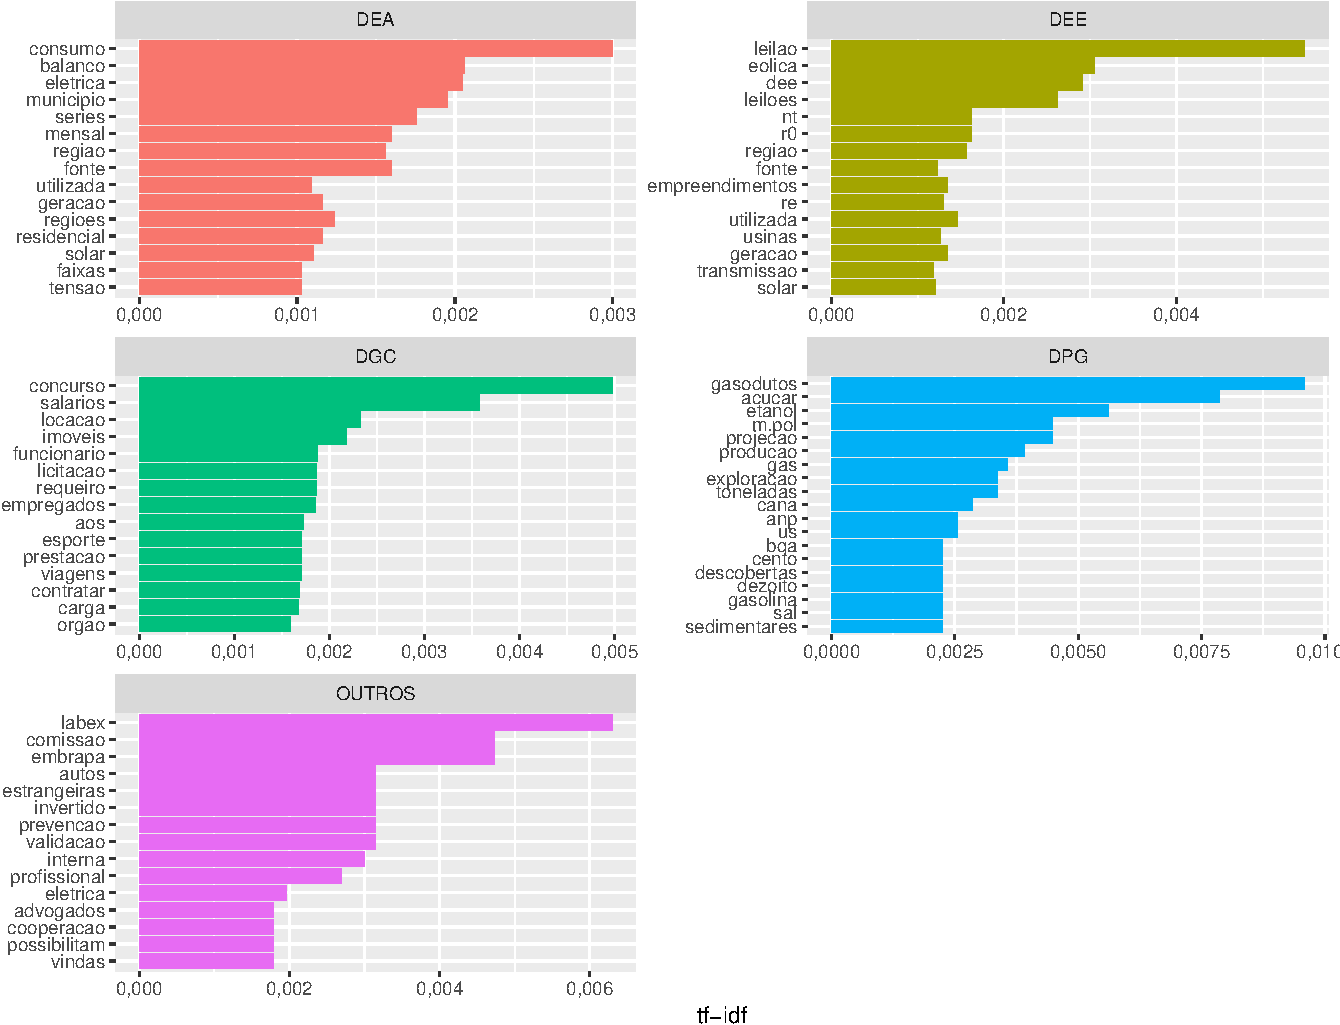
\includegraphics{markdown_v24_files/figure-latex/unnamed-chunk-40-1.pdf}

\begin{Shaded}
\begin{Highlighting}[]
\CommentTok{#dev.off()}
\end{Highlighting}
\end{Shaded}

\subsubsection{Stopwords}\label{stopwords}

Com o arquivo de \texttt{stopwords}previamente inserido vamos,
primeiramente, transforma-lo em um data\_frame a fim de futuramente
utilizá-lo para extrair do texto palavras em comum.

\paragraph{\texorpdfstring{Freq. de palavras sem \textbf{stopwords} por
diretoria}{Freq. de palavras sem stopwords por diretoria}}\label{freq.-de-palavras-sem-stopwords-por-diretoria}

\begin{Shaded}
\begin{Highlighting}[]
\NormalTok{mystopwords <-}\StringTok{ }\KeywordTok{data_frame}\NormalTok{(}\DataTypeTok{palavra =}\NormalTok{ stopwords_pt)}
\end{Highlighting}
\end{Shaded}

\begin{verbatim}
## Warning: `data_frame()` is deprecated, use `tibble()`.
## This warning is displayed once per session.
\end{verbatim}

\begin{Shaded}
\begin{Highlighting}[]
\NormalTok{diretoria_palavras_noSTOP <-}\StringTok{ }\KeywordTok{anti_join}\NormalTok{(diretoria_palavras_stem3, mystopwords, }\DataTypeTok{by =} \StringTok{"palavra"}\NormalTok{)}
\CommentTok{#View(head(diretoria_palavras_noSTOP))}
\end{Highlighting}
\end{Shaded}

\begin{Shaded}
\begin{Highlighting}[]
\CommentTok{#diretoria_palavras_noSTOP_noSTOP}
\NormalTok{plot_diretoria_palavras_noSTOP <-}\StringTok{ }\NormalTok{diretoria_palavras_noSTOP }\OperatorTok
\StringTok{  }\KeywordTok{bind_tf_idf}\NormalTok{(palavra, DIRETORIA, n) }\OperatorTok
\StringTok{  }\KeywordTok{arrange}\NormalTok{(}\KeywordTok{desc}\NormalTok{(tf_idf)) }\OperatorTok
\StringTok{  }\KeywordTok{mutate}\NormalTok{(}\DataTypeTok{word =} \KeywordTok{factor}\NormalTok{(palavra, }\DataTypeTok{levels =} \KeywordTok{rev}\NormalTok{(}\KeywordTok{unique}\NormalTok{(palavra)))) }\OperatorTok
\StringTok{  }\KeywordTok{mutate}\NormalTok{(}\DataTypeTok{DIRETORIA =} \KeywordTok{factor}\NormalTok{(DIRETORIA, }\DataTypeTok{levels =} \KeywordTok{c}\NormalTok{(}\StringTok{"DEA"}\NormalTok{,}
                                                  \StringTok{"DEE"}\NormalTok{,}
                                                  \StringTok{"DGC"}\NormalTok{,}
                                                  \StringTok{"DPG"}\NormalTok{,}
                                                  \StringTok{"OUTROS"}\NormalTok{)))}
\CommentTok{#plot_diretoria_palavras_noSTOP}
\CommentTok{#windows.options(width=10, height=10)}
\CommentTok{#jpeg("03_freq_palavras_dir_nostop.jpeg")}
\NormalTok{plot_diretoria_palavras_noSTOP }\OperatorTok
\KeywordTok{group_by}\NormalTok{(DIRETORIA) }\OperatorTok
\KeywordTok{top_n}\NormalTok{(}\DecValTok{15}\NormalTok{, tf_idf) }\OperatorTok
\KeywordTok{ungroup}\NormalTok{() }\OperatorTok
\KeywordTok{mutate}\NormalTok{(}\DataTypeTok{palavra =} \KeywordTok{reorder}\NormalTok{(palavra, tf_idf)) }\OperatorTok
\KeywordTok{ggplot}\NormalTok{(}\KeywordTok{aes}\NormalTok{(palavra, tf_idf, }\DataTypeTok{fill =}\NormalTok{ DIRETORIA)) }\OperatorTok{+}
\KeywordTok{geom_col}\NormalTok{(}\DataTypeTok{show.legend =} \OtherTok{FALSE}\NormalTok{) }\OperatorTok{+}
\KeywordTok{labs}\NormalTok{(}\DataTypeTok{x =} \OtherTok{NULL}\NormalTok{, }\DataTypeTok{y =} \StringTok{"tf-idf"}\NormalTok{) }\OperatorTok{+}
\KeywordTok{facet_wrap}\NormalTok{(}\OperatorTok{~}\NormalTok{DIRETORIA, }\DataTypeTok{ncol =} \DecValTok{2}\NormalTok{, }\DataTypeTok{scales =} \StringTok{"free"}\NormalTok{) }\OperatorTok{+}
\KeywordTok{coord_flip}\NormalTok{() }\OperatorTok{+}\StringTok{ }
\KeywordTok{scale_y_continuous}\NormalTok{(}\DataTypeTok{labels=}\NormalTok{gcomma)}
\end{Highlighting}
\end{Shaded}

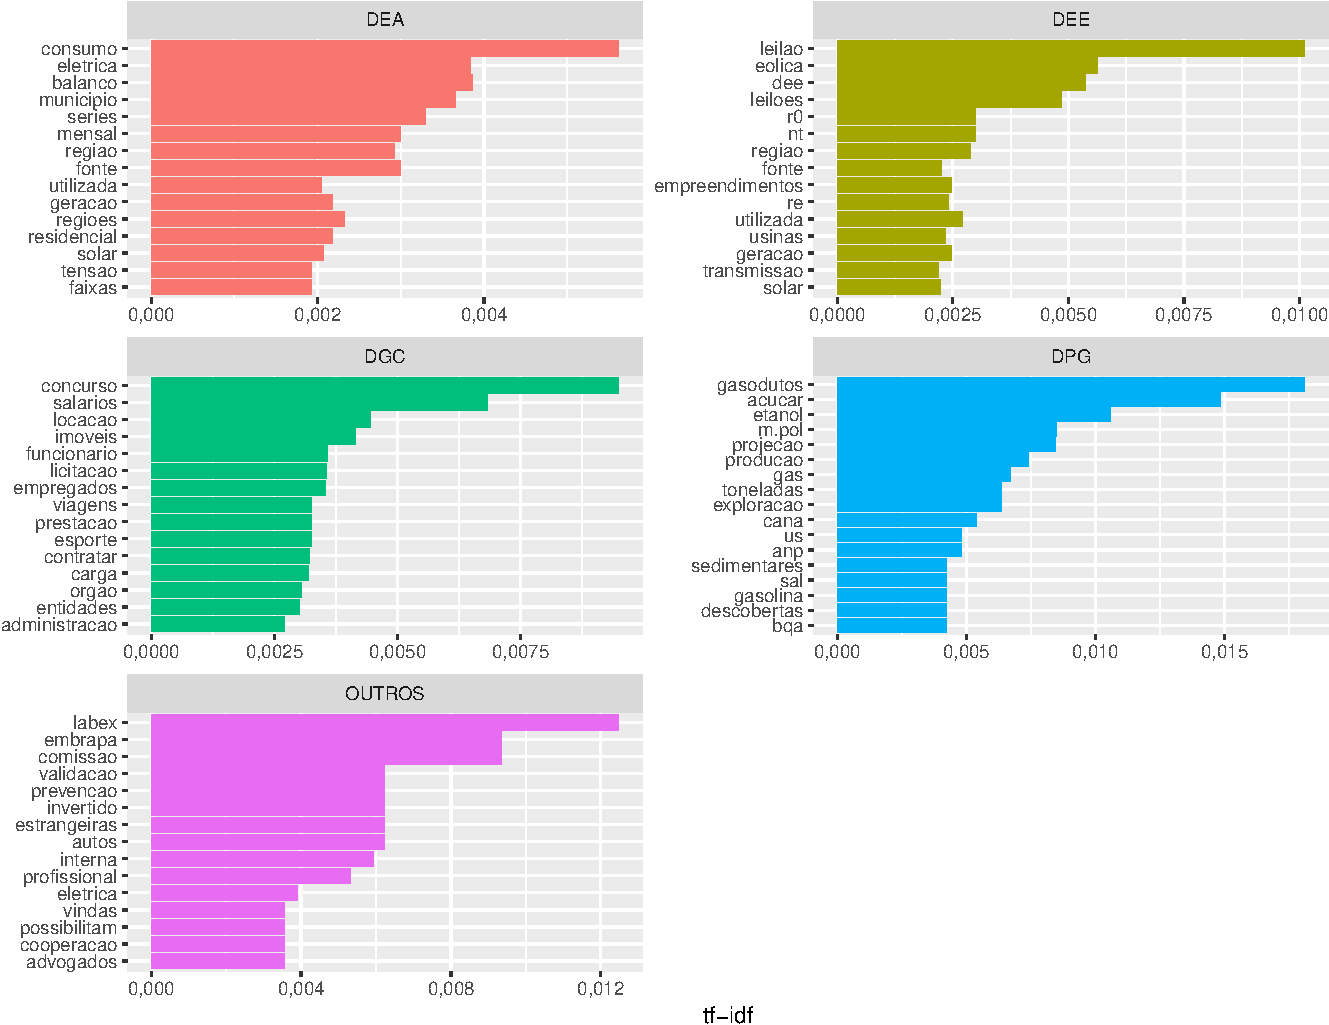
\includegraphics{markdown_v24_files/figure-latex/03_freq_palavras_dir_nostop-1.pdf}

\begin{Shaded}
\begin{Highlighting}[]
\CommentTok{#dev.off()}
\end{Highlighting}
\end{Shaded}

\paragraph{Gráficos de comparação de frequência de palavras por
diretorias (2 a
2)}\label{graficos-de-comparacao-de-frequencia-de-palavras-por-diretorias-2-a-2}

\texttt{COM\ STOPWORDS}

É importante ressaltar que os gráficos a seguir mostram, apenas, a
comparação de frequência de palavras existentes em ambas diretorias. Ou
seja, palavras existentes em apenas uma diretoria serão desconsideradas
para a geração destes.

\begin{Shaded}
\begin{Highlighting}[]
\NormalTok{PROP_PALAVRA =}\StringTok{ }\NormalTok{diretoria_palavras_noSTOP }\OperatorTok
\StringTok{    }\CommentTok{#mutate(palavra = str_extract(palavra, "[a-z']+")) %>%}
\StringTok{    }\KeywordTok{mutate}\NormalTok{(}\DataTypeTok{proportion =}\NormalTok{ n }\OperatorTok{/}\StringTok{ }\KeywordTok{sum}\NormalTok{(n)) }\OperatorTok
\StringTok{    }\KeywordTok{select}\NormalTok{(}\OperatorTok{-}\NormalTok{n) }\OperatorTok
\StringTok{    }\KeywordTok{spread}\NormalTok{(DIRETORIA, proportion)}
\end{Highlighting}
\end{Shaded}

\begin{itemize}
\tightlist
\item
  DEE X DEA
\end{itemize}

\begin{Shaded}
\begin{Highlighting}[]
\NormalTok{freq00 <-}\StringTok{ }\NormalTok{PROP_PALAVRA }\OperatorTok
\StringTok{    }\KeywordTok{gather}\NormalTok{(DIRETORIA, proportion, }\KeywordTok{c}\NormalTok{(}\StringTok{`}\DataTypeTok{DEA}\StringTok{`}\NormalTok{))}
  
  \KeywordTok{library}\NormalTok{(scales)}
  \CommentTok{# expect a warning about rows with missing values being removed}
  \KeywordTok{ggplot}\NormalTok{(freq00, }\KeywordTok{aes}\NormalTok{(}\DataTypeTok{x =}\NormalTok{ proportion, }\DataTypeTok{y =} \StringTok{`}\DataTypeTok{DEE}\StringTok{`}\NormalTok{,}
                        \DataTypeTok{color =} \KeywordTok{abs}\NormalTok{(}\StringTok{`}\DataTypeTok{DEE}\StringTok{`} \OperatorTok{-}\StringTok{ }\NormalTok{proportion))) }\OperatorTok{+}
\StringTok{    }\KeywordTok{geom_abline}\NormalTok{(}\DataTypeTok{color =} \StringTok{"gray40"}\NormalTok{, }\DataTypeTok{lty =} \DecValTok{2}\NormalTok{) }\OperatorTok{+}
\StringTok{    }\KeywordTok{geom_jitter}\NormalTok{(}\DataTypeTok{alpha =} \FloatTok{0.1}\NormalTok{, }\DataTypeTok{size =} \FloatTok{2.5}\NormalTok{, }\DataTypeTok{width =} \FloatTok{0.3}\NormalTok{, }\DataTypeTok{height =} \FloatTok{0.3}\NormalTok{) }\OperatorTok{+}
\StringTok{    }\KeywordTok{geom_text}\NormalTok{(}\KeywordTok{aes}\NormalTok{(}\DataTypeTok{label =}\NormalTok{ palavra), }\DataTypeTok{check_overlap =} \OtherTok{TRUE}\NormalTok{, }\DataTypeTok{vjust =} \FloatTok{1.5}\NormalTok{) }\OperatorTok{+}
\StringTok{    }\KeywordTok{scale_x_log10}\NormalTok{(}\DataTypeTok{labels =} \KeywordTok{percent_format}\NormalTok{(}\DataTypeTok{big.mark =} \StringTok{"."}\NormalTok{, }\DataTypeTok{decimal.mark =} \StringTok{","}\NormalTok{, }\DataTypeTok{accuracy =} \DecValTok{1}\NormalTok{), }\DataTypeTok{limits =} \KeywordTok{c}\NormalTok{(}\OtherTok{NA}\NormalTok{, }\FloatTok{0.01}\NormalTok{)) }\OperatorTok{+}
\StringTok{    }\KeywordTok{scale_y_log10}\NormalTok{(}\DataTypeTok{labels =} \KeywordTok{percent_format}\NormalTok{(}\DataTypeTok{big.mark =} \StringTok{"."}\NormalTok{, }\DataTypeTok{decimal.mark =} \StringTok{","}\NormalTok{, }\DataTypeTok{accuracy =} \DecValTok{1}\NormalTok{), }\DataTypeTok{limits =} \KeywordTok{c}\NormalTok{(}\OtherTok{NA}\NormalTok{, }\FloatTok{0.01}\NormalTok{)) }\OperatorTok{+}
\StringTok{    }\KeywordTok{scale_color_gradient}\NormalTok{(}\DataTypeTok{limits =} \KeywordTok{c}\NormalTok{(}\DecValTok{0}\NormalTok{, }\FloatTok{0.001}\NormalTok{),}
                         \DataTypeTok{low =} \StringTok{"darkslategray4"}\NormalTok{, }\DataTypeTok{high =} \StringTok{"gray75"}\NormalTok{) }\OperatorTok{+}
\StringTok{    }\KeywordTok{facet_wrap}\NormalTok{(}\OperatorTok{~}\NormalTok{DIRETORIA, }\DataTypeTok{ncol =} \DecValTok{1}\NormalTok{) }\OperatorTok{+}
\StringTok{    }\KeywordTok{theme}\NormalTok{(}\DataTypeTok{legend.position=}\StringTok{"none"}\NormalTok{) }\OperatorTok{+}
\StringTok{    }\KeywordTok{labs}\NormalTok{(}\DataTypeTok{y =} \StringTok{"DEE"}\NormalTok{, }\DataTypeTok{x =} \OtherTok{NULL}\NormalTok{)}
\end{Highlighting}
\end{Shaded}

\begin{verbatim}
## Warning: Removed 2824 rows containing missing values (geom_point).
\end{verbatim}

\begin{verbatim}
## Warning: Removed 2823 rows containing missing values (geom_text).
\end{verbatim}

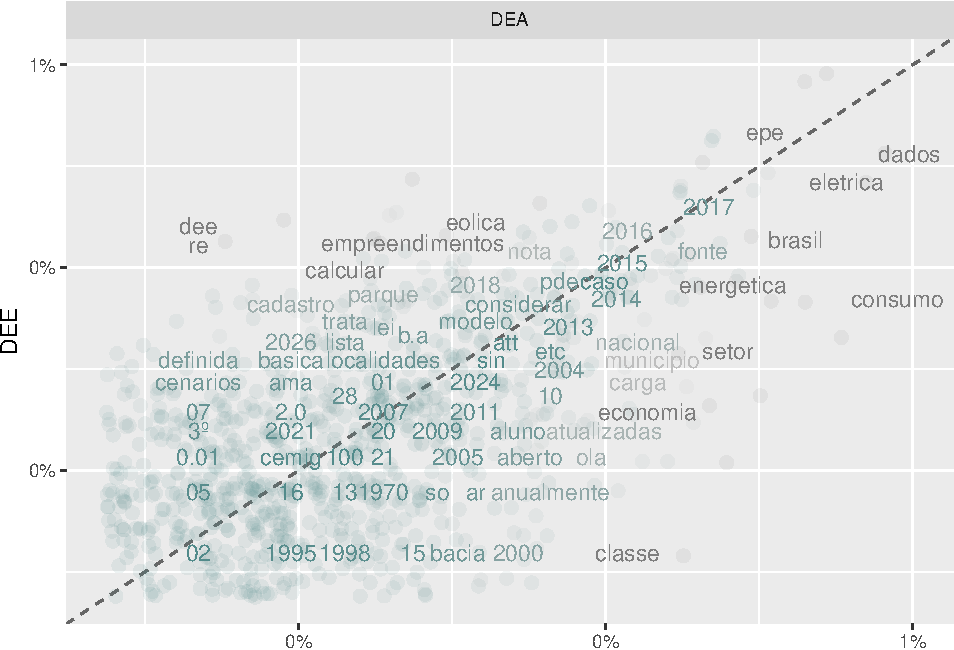
\includegraphics{markdown_v24_files/figure-latex/unnamed-chunk-51-1.pdf}

\begin{Shaded}
\begin{Highlighting}[]
\KeywordTok{cor.test}\NormalTok{(}\DataTypeTok{data =}\NormalTok{ freq00[freq00}\OperatorTok{$}\NormalTok{DIRETORIA }\OperatorTok{==}\StringTok{ "DEA"}\NormalTok{,],}
             \OperatorTok{~}\StringTok{ }\NormalTok{proportion }\OperatorTok{+}\StringTok{ `}\DataTypeTok{DEE}\StringTok{`}\NormalTok{)}
\end{Highlighting}
\end{Shaded}

\begin{verbatim}
## 
##  Pearson's product-moment correlation
## 
## data:  proportion and DEE
## t = 30.221, df = 890, p-value < 2.2e-16
## alternative hypothesis: true correlation is not equal to 0
## 95 percent confidence interval:
##  0.6776757 0.7426100
## sample estimates:
##       cor 
## 0.7116595
\end{verbatim}

\begin{itemize}
\tightlist
\item
  DEE X DPG
\end{itemize}

\begin{Shaded}
\begin{Highlighting}[]
\NormalTok{freq01 <-}\StringTok{ }\NormalTok{PROP_PALAVRA }\OperatorTok
\StringTok{    }\KeywordTok{gather}\NormalTok{(DIRETORIA, proportion, }\KeywordTok{c}\NormalTok{(}\StringTok{`}\DataTypeTok{DPG}\StringTok{`}\NormalTok{))}
  
  \KeywordTok{library}\NormalTok{(scales)}
  \CommentTok{# expect a warning about rows with missing values being removed}
  \KeywordTok{ggplot}\NormalTok{(freq01, }\KeywordTok{aes}\NormalTok{(}\DataTypeTok{x =}\NormalTok{ proportion, }\DataTypeTok{y =} \StringTok{`}\DataTypeTok{DEE}\StringTok{`}\NormalTok{,}
                        \DataTypeTok{color =} \KeywordTok{abs}\NormalTok{(}\StringTok{`}\DataTypeTok{DEE}\StringTok{`} \OperatorTok{-}\StringTok{ }\NormalTok{proportion))) }\OperatorTok{+}
\StringTok{    }\KeywordTok{geom_abline}\NormalTok{(}\DataTypeTok{color =} \StringTok{"gray40"}\NormalTok{, }\DataTypeTok{lty =} \DecValTok{2}\NormalTok{) }\OperatorTok{+}
\StringTok{    }\KeywordTok{geom_jitter}\NormalTok{(}\DataTypeTok{alpha =} \FloatTok{0.1}\NormalTok{, }\DataTypeTok{size =} \FloatTok{2.5}\NormalTok{, }\DataTypeTok{width =} \FloatTok{0.3}\NormalTok{, }\DataTypeTok{height =} \FloatTok{0.3}\NormalTok{) }\OperatorTok{+}
\StringTok{    }\KeywordTok{geom_text}\NormalTok{(}\KeywordTok{aes}\NormalTok{(}\DataTypeTok{label =}\NormalTok{ palavra), }\DataTypeTok{check_overlap =} \OtherTok{TRUE}\NormalTok{, }\DataTypeTok{vjust =} \FloatTok{1.5}\NormalTok{) }\OperatorTok{+}
\StringTok{    }\KeywordTok{scale_x_log10}\NormalTok{(}\DataTypeTok{labels =} \KeywordTok{percent_format}\NormalTok{(}\DataTypeTok{big.mark =} \StringTok{"."}\NormalTok{, }\DataTypeTok{decimal.mark =} \StringTok{","}\NormalTok{, }\DataTypeTok{accuracy =} \DecValTok{1}\NormalTok{), }\DataTypeTok{limits =} \KeywordTok{c}\NormalTok{(}\OtherTok{NA}\NormalTok{, }\FloatTok{0.01}\NormalTok{)) }\OperatorTok{+}
\StringTok{    }\KeywordTok{scale_y_log10}\NormalTok{(}\DataTypeTok{labels =} \KeywordTok{percent_format}\NormalTok{(}\DataTypeTok{big.mark =} \StringTok{"."}\NormalTok{, }\DataTypeTok{decimal.mark =} \StringTok{","}\NormalTok{, }\DataTypeTok{accuracy =} \DecValTok{1}\NormalTok{), }\DataTypeTok{limits =} \KeywordTok{c}\NormalTok{(}\OtherTok{NA}\NormalTok{, }\FloatTok{0.01}\NormalTok{)) }\OperatorTok{+}
\StringTok{    }\KeywordTok{scale_color_gradient}\NormalTok{(}\DataTypeTok{limits =} \KeywordTok{c}\NormalTok{(}\DecValTok{0}\NormalTok{, }\FloatTok{0.001}\NormalTok{),}
                         \DataTypeTok{low =} \StringTok{"darkslategray4"}\NormalTok{, }\DataTypeTok{high =} \StringTok{"gray75"}\NormalTok{) }\OperatorTok{+}
\StringTok{    }\KeywordTok{facet_wrap}\NormalTok{(}\OperatorTok{~}\NormalTok{DIRETORIA, }\DataTypeTok{ncol =} \DecValTok{1}\NormalTok{) }\OperatorTok{+}
\StringTok{    }\KeywordTok{theme}\NormalTok{(}\DataTypeTok{legend.position=}\StringTok{"none"}\NormalTok{) }\OperatorTok{+}
\StringTok{    }\KeywordTok{labs}\NormalTok{(}\DataTypeTok{y =} \StringTok{"DEE"}\NormalTok{, }\DataTypeTok{x =} \OtherTok{NULL}\NormalTok{)}
\end{Highlighting}
\end{Shaded}

\begin{verbatim}
## Warning: Removed 3438 rows containing missing values (geom_point).
\end{verbatim}

\begin{verbatim}
## Warning: Removed 3438 rows containing missing values (geom_text).
\end{verbatim}

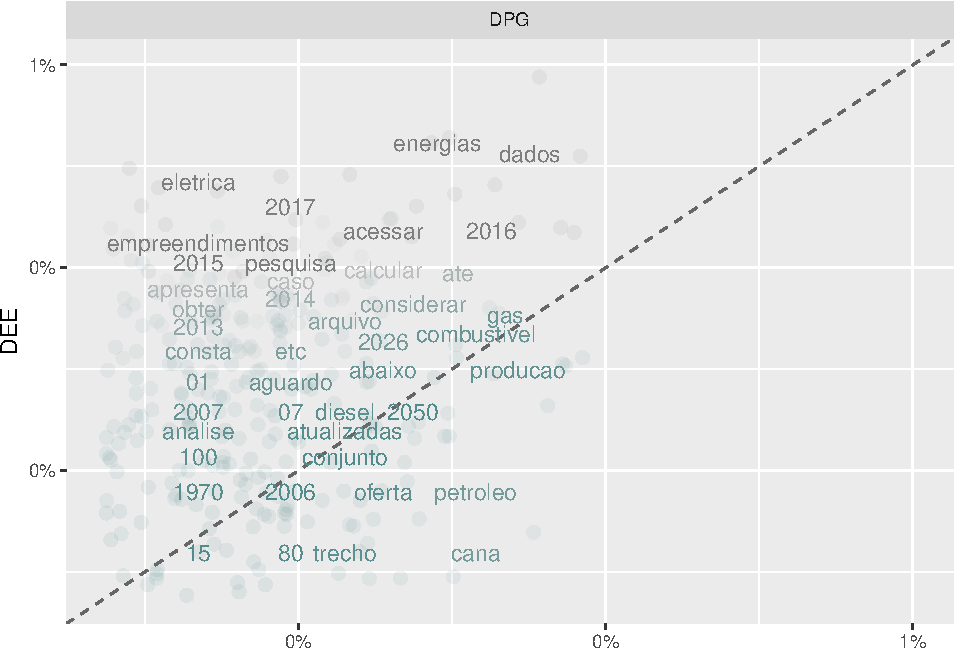
\includegraphics{markdown_v24_files/figure-latex/unnamed-chunk-53-1.pdf}

\begin{Shaded}
\begin{Highlighting}[]
\KeywordTok{cor.test}\NormalTok{(}\DataTypeTok{data =}\NormalTok{ freq01[freq01}\OperatorTok{$}\NormalTok{DIRETORIA }\OperatorTok{==}\StringTok{ "DPG"}\NormalTok{,],}
             \OperatorTok{~}\StringTok{ }\NormalTok{proportion }\OperatorTok{+}\StringTok{ `}\DataTypeTok{DEE}\StringTok{`}\NormalTok{)}
\end{Highlighting}
\end{Shaded}

\begin{verbatim}
## 
##  Pearson's product-moment correlation
## 
## data:  proportion and DEE
## t = 7.7037, df = 275, p-value = 2.406e-13
## alternative hypothesis: true correlation is not equal to 0
## 95 percent confidence interval:
##  0.3193085 0.5136596
## sample estimates:
##       cor 
## 0.4213092
\end{verbatim}

\begin{Shaded}
\begin{Highlighting}[]
\FunctionTok{Warning messages:}
\FunctionTok{1:}\AttributeTok{ Removed 4235 rows containing missing values (geom_point). }
\FunctionTok{2:}\AttributeTok{ Removed 4236 rows containing missing values (geom_text). }
\end{Highlighting}
\end{Shaded}

\begin{itemize}
\tightlist
\item
  DEE X DGC
\end{itemize}

\begin{Shaded}
\begin{Highlighting}[]
\NormalTok{freq02 <-}\StringTok{ }\NormalTok{PROP_PALAVRA }\OperatorTok
\StringTok{    }\KeywordTok{gather}\NormalTok{(DIRETORIA, proportion, }\KeywordTok{c}\NormalTok{(}\StringTok{`}\DataTypeTok{DGC}\StringTok{`}\NormalTok{))}
  
  \KeywordTok{library}\NormalTok{(scales)}
  \CommentTok{# expect a warning about rows with missing values being removed}
  \KeywordTok{ggplot}\NormalTok{(freq02, }\KeywordTok{aes}\NormalTok{(}\DataTypeTok{x =}\NormalTok{ proportion, }\DataTypeTok{y =} \StringTok{`}\DataTypeTok{DEE}\StringTok{`}\NormalTok{,}
                        \DataTypeTok{color =} \KeywordTok{abs}\NormalTok{(}\StringTok{`}\DataTypeTok{DEE}\StringTok{`} \OperatorTok{-}\StringTok{ }\NormalTok{proportion))) }\OperatorTok{+}
\StringTok{    }\KeywordTok{geom_abline}\NormalTok{(}\DataTypeTok{color =} \StringTok{"gray40"}\NormalTok{, }\DataTypeTok{lty =} \DecValTok{2}\NormalTok{) }\OperatorTok{+}
\StringTok{    }\KeywordTok{geom_jitter}\NormalTok{(}\DataTypeTok{alpha =} \FloatTok{0.1}\NormalTok{, }\DataTypeTok{size =} \FloatTok{2.5}\NormalTok{, }\DataTypeTok{width =} \FloatTok{0.3}\NormalTok{, }\DataTypeTok{height =} \FloatTok{0.3}\NormalTok{) }\OperatorTok{+}
\StringTok{    }\KeywordTok{geom_text}\NormalTok{(}\KeywordTok{aes}\NormalTok{(}\DataTypeTok{label =}\NormalTok{ palavra), }\DataTypeTok{check_overlap =} \OtherTok{TRUE}\NormalTok{, }\DataTypeTok{vjust =} \FloatTok{1.5}\NormalTok{) }\OperatorTok{+}
\StringTok{    }\KeywordTok{scale_x_log10}\NormalTok{(}\DataTypeTok{labels =} \KeywordTok{percent_format}\NormalTok{(}\DataTypeTok{big.mark =} \StringTok{"."}\NormalTok{, }\DataTypeTok{decimal.mark =} \StringTok{","}\NormalTok{, }\DataTypeTok{accuracy =} \DecValTok{1}\NormalTok{), }\DataTypeTok{limits =} \KeywordTok{c}\NormalTok{(}\OtherTok{NA}\NormalTok{, }\FloatTok{0.01}\NormalTok{)) }\OperatorTok{+}
\StringTok{    }\KeywordTok{scale_y_log10}\NormalTok{(}\DataTypeTok{labels =} \KeywordTok{percent_format}\NormalTok{(}\DataTypeTok{big.mark =} \StringTok{"."}\NormalTok{, }\DataTypeTok{decimal.mark =} \StringTok{","}\NormalTok{, }\DataTypeTok{accuracy =} \DecValTok{1}\NormalTok{), }\DataTypeTok{limits =} \KeywordTok{c}\NormalTok{(}\OtherTok{NA}\NormalTok{, }\FloatTok{0.01}\NormalTok{)) }\OperatorTok{+}
\StringTok{    }\KeywordTok{scale_color_gradient}\NormalTok{(}\DataTypeTok{limits =} \KeywordTok{c}\NormalTok{(}\DecValTok{0}\NormalTok{, }\FloatTok{0.001}\NormalTok{),}
                         \DataTypeTok{low =} \StringTok{"darkslategray4"}\NormalTok{, }\DataTypeTok{high =} \StringTok{"gray75"}\NormalTok{) }\OperatorTok{+}
\StringTok{    }\KeywordTok{facet_wrap}\NormalTok{(}\OperatorTok{~}\NormalTok{DIRETORIA, }\DataTypeTok{ncol =} \DecValTok{1}\NormalTok{) }\OperatorTok{+}
\StringTok{    }\KeywordTok{theme}\NormalTok{(}\DataTypeTok{legend.position=}\StringTok{"none"}\NormalTok{) }\OperatorTok{+}
\StringTok{    }\KeywordTok{labs}\NormalTok{(}\DataTypeTok{y =} \StringTok{"DEE"}\NormalTok{, }\DataTypeTok{x =} \OtherTok{NULL}\NormalTok{)}
\end{Highlighting}
\end{Shaded}

\begin{verbatim}
## Warning: Removed 3075 rows containing missing values (geom_point).
\end{verbatim}

\begin{verbatim}
## Warning: Removed 3075 rows containing missing values (geom_text).
\end{verbatim}

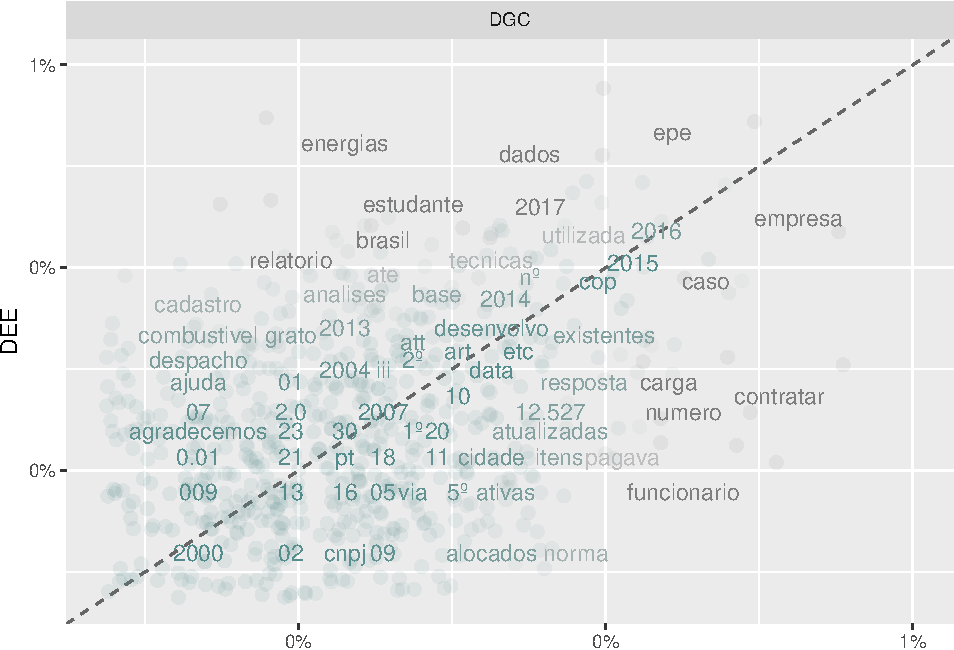
\includegraphics{markdown_v24_files/figure-latex/unnamed-chunk-55-1.pdf}

\begin{Shaded}
\begin{Highlighting}[]
\KeywordTok{cor.test}\NormalTok{(}\DataTypeTok{data =}\NormalTok{ freq02[freq02}\OperatorTok{$}\NormalTok{DIRETORIA }\OperatorTok{==}\StringTok{ "DGC"}\NormalTok{,],}
             \OperatorTok{~}\StringTok{ }\NormalTok{proportion }\OperatorTok{+}\StringTok{ `}\DataTypeTok{DEE}\StringTok{`}\NormalTok{)}
\end{Highlighting}
\end{Shaded}

\begin{verbatim}
## 
##  Pearson's product-moment correlation
## 
## data:  proportion and DEE
## t = 10.85, df = 638, p-value < 2.2e-16
## alternative hypothesis: true correlation is not equal to 0
## 95 percent confidence interval:
##  0.3271860 0.4581655
## sample estimates:
##      cor 
## 0.394679
\end{verbatim}

\begin{Shaded}
\begin{Highlighting}[]
\FunctionTok{Warning messages:}
\FunctionTok{1:}\AttributeTok{ Removed 3794 rows containing missing values (geom_point). }
\FunctionTok{2:}\AttributeTok{ Removed 3795 rows containing missing values (geom_text).}
\end{Highlighting}
\end{Shaded}

\begin{itemize}
\tightlist
\item
  DEE X OUTROS
\end{itemize}

\begin{Shaded}
\begin{Highlighting}[]
\NormalTok{freq03 <-}\StringTok{ }\NormalTok{PROP_PALAVRA }\OperatorTok
\StringTok{    }\KeywordTok{gather}\NormalTok{(DIRETORIA, proportion, }\KeywordTok{c}\NormalTok{(}\StringTok{`}\DataTypeTok{OUTROS}\StringTok{`}\NormalTok{))}
  
  \KeywordTok{library}\NormalTok{(scales)}
  \CommentTok{# expect a warning about rows with missing values being removed}
  \KeywordTok{ggplot}\NormalTok{(freq03, }\KeywordTok{aes}\NormalTok{(}\DataTypeTok{x =}\NormalTok{ proportion, }\DataTypeTok{y =} \StringTok{`}\DataTypeTok{DEE}\StringTok{`}\NormalTok{,}
                        \DataTypeTok{color =} \KeywordTok{abs}\NormalTok{(}\StringTok{`}\DataTypeTok{DEE}\StringTok{`} \OperatorTok{-}\StringTok{ }\NormalTok{proportion))) }\OperatorTok{+}
\StringTok{    }\KeywordTok{geom_abline}\NormalTok{(}\DataTypeTok{color =} \StringTok{"gray40"}\NormalTok{, }\DataTypeTok{lty =} \DecValTok{2}\NormalTok{) }\OperatorTok{+}
\StringTok{    }\KeywordTok{geom_jitter}\NormalTok{(}\DataTypeTok{alpha =} \FloatTok{0.1}\NormalTok{, }\DataTypeTok{size =} \FloatTok{2.5}\NormalTok{, }\DataTypeTok{width =} \FloatTok{0.3}\NormalTok{, }\DataTypeTok{height =} \FloatTok{0.3}\NormalTok{) }\OperatorTok{+}
\StringTok{    }\KeywordTok{geom_text}\NormalTok{(}\KeywordTok{aes}\NormalTok{(}\DataTypeTok{label =}\NormalTok{ palavra), }\DataTypeTok{check_overlap =} \OtherTok{TRUE}\NormalTok{, }\DataTypeTok{vjust =} \FloatTok{1.5}\NormalTok{) }\OperatorTok{+}
\StringTok{    }\KeywordTok{scale_x_log10}\NormalTok{(}\DataTypeTok{labels =} \KeywordTok{percent_format}\NormalTok{(}\DataTypeTok{big.mark =} \StringTok{"."}\NormalTok{, }\DataTypeTok{decimal.mark =} \StringTok{","}\NormalTok{, }\DataTypeTok{accuracy =} \DecValTok{1}\NormalTok{), }\DataTypeTok{limits =} \KeywordTok{c}\NormalTok{(}\OtherTok{NA}\NormalTok{, }\FloatTok{0.01}\NormalTok{)) }\OperatorTok{+}
\StringTok{    }\KeywordTok{scale_y_log10}\NormalTok{(}\DataTypeTok{labels =} \KeywordTok{percent_format}\NormalTok{(}\DataTypeTok{big.mark =} \StringTok{"."}\NormalTok{, }\DataTypeTok{decimal.mark =} \StringTok{","}\NormalTok{, }\DataTypeTok{accuracy =} \DecValTok{1}\NormalTok{), }\DataTypeTok{limits =} \KeywordTok{c}\NormalTok{(}\OtherTok{NA}\NormalTok{, }\FloatTok{0.01}\NormalTok{)) }\OperatorTok{+}
\StringTok{    }\KeywordTok{scale_color_gradient}\NormalTok{(}\DataTypeTok{limits =} \KeywordTok{c}\NormalTok{(}\DecValTok{0}\NormalTok{, }\FloatTok{0.001}\NormalTok{),}
                         \DataTypeTok{low =} \StringTok{"darkslategray4"}\NormalTok{, }\DataTypeTok{high =} \StringTok{"gray75"}\NormalTok{) }\OperatorTok{+}
\StringTok{    }\KeywordTok{facet_wrap}\NormalTok{(}\OperatorTok{~}\NormalTok{DIRETORIA, }\DataTypeTok{ncol =} \DecValTok{1}\NormalTok{) }\OperatorTok{+}
\StringTok{    }\KeywordTok{theme}\NormalTok{(}\DataTypeTok{legend.position=}\StringTok{"none"}\NormalTok{) }\OperatorTok{+}
\StringTok{    }\KeywordTok{labs}\NormalTok{(}\DataTypeTok{y =} \StringTok{"DEE"}\NormalTok{, }\DataTypeTok{x =} \OtherTok{NULL}\NormalTok{)}
\end{Highlighting}
\end{Shaded}

\begin{verbatim}
## Warning: Removed 3477 rows containing missing values (geom_point).
\end{verbatim}

\begin{verbatim}
## Warning: Removed 3477 rows containing missing values (geom_text).
\end{verbatim}

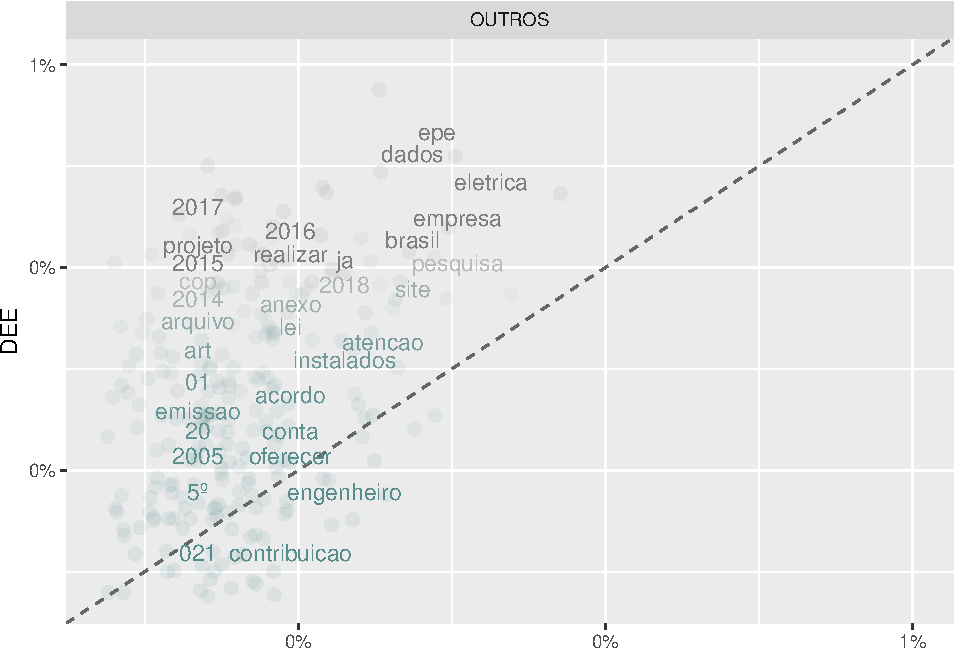
\includegraphics{markdown_v24_files/figure-latex/unnamed-chunk-57-1.pdf}

\begin{Shaded}
\begin{Highlighting}[]
\KeywordTok{cor.test}\NormalTok{(}\DataTypeTok{data =}\NormalTok{ freq03[freq03}\OperatorTok{$}\NormalTok{DIRETORIA }\OperatorTok{==}\StringTok{ "OUTROS"}\NormalTok{,],}
             \OperatorTok{~}\StringTok{ }\NormalTok{proportion }\OperatorTok{+}\StringTok{ `}\DataTypeTok{DEE}\StringTok{`}\NormalTok{)}
\end{Highlighting}
\end{Shaded}

\begin{verbatim}
## 
##  Pearson's product-moment correlation
## 
## data:  proportion and DEE
## t = 12.789, df = 236, p-value < 2.2e-16
## alternative hypothesis: true correlation is not equal to 0
## 95 percent confidence interval:
##  0.5580327 0.7092533
## sample estimates:
##       cor 
## 0.6397945
\end{verbatim}

\begin{Shaded}
\begin{Highlighting}[]
\FunctionTok{Warning messages:}
\FunctionTok{1:}\AttributeTok{ Removed 4273 rows containing missing values (geom_point). }
\FunctionTok{2:}\AttributeTok{ Removed 4274 rows containing missing values (geom_text).}
\end{Highlighting}
\end{Shaded}

\begin{itemize}
\tightlist
\item
  DEA X DPG
\end{itemize}

\begin{Shaded}
\begin{Highlighting}[]
\NormalTok{freq04 <-}\StringTok{ }\NormalTok{PROP_PALAVRA }\OperatorTok
\StringTok{    }\KeywordTok{gather}\NormalTok{(DIRETORIA, proportion, }\KeywordTok{c}\NormalTok{(}\StringTok{`}\DataTypeTok{DPG}\StringTok{`}\NormalTok{))}
  
  \KeywordTok{library}\NormalTok{(scales)}
  \CommentTok{# expect a warning about rows with missing values being removed}
  \KeywordTok{ggplot}\NormalTok{(freq04, }\KeywordTok{aes}\NormalTok{(}\DataTypeTok{x =}\NormalTok{ proportion, }\DataTypeTok{y =} \StringTok{`}\DataTypeTok{DEA}\StringTok{`}\NormalTok{,}
                        \DataTypeTok{color =} \KeywordTok{abs}\NormalTok{(}\StringTok{`}\DataTypeTok{DEA}\StringTok{`} \OperatorTok{-}\StringTok{ }\NormalTok{proportion))) }\OperatorTok{+}
\StringTok{    }\KeywordTok{geom_abline}\NormalTok{(}\DataTypeTok{color =} \StringTok{"gray40"}\NormalTok{, }\DataTypeTok{lty =} \DecValTok{2}\NormalTok{) }\OperatorTok{+}
\StringTok{    }\KeywordTok{geom_jitter}\NormalTok{(}\DataTypeTok{alpha =} \FloatTok{0.1}\NormalTok{, }\DataTypeTok{size =} \FloatTok{2.5}\NormalTok{, }\DataTypeTok{width =} \FloatTok{0.3}\NormalTok{, }\DataTypeTok{height =} \FloatTok{0.3}\NormalTok{) }\OperatorTok{+}
\StringTok{    }\KeywordTok{geom_text}\NormalTok{(}\KeywordTok{aes}\NormalTok{(}\DataTypeTok{label =}\NormalTok{ palavra), }\DataTypeTok{check_overlap =} \OtherTok{TRUE}\NormalTok{, }\DataTypeTok{vjust =} \FloatTok{1.5}\NormalTok{) }\OperatorTok{+}
\StringTok{    }\KeywordTok{scale_x_log10}\NormalTok{(}\DataTypeTok{labels =} \KeywordTok{percent_format}\NormalTok{(}\DataTypeTok{big.mark =} \StringTok{"."}\NormalTok{, }\DataTypeTok{decimal.mark =} \StringTok{","}\NormalTok{, }\DataTypeTok{accuracy =} \DecValTok{1}\NormalTok{), }\DataTypeTok{limits =} \KeywordTok{c}\NormalTok{(}\OtherTok{NA}\NormalTok{, }\FloatTok{0.01}\NormalTok{)) }\OperatorTok{+}
\StringTok{    }\KeywordTok{scale_y_log10}\NormalTok{(}\DataTypeTok{labels =} \KeywordTok{percent_format}\NormalTok{(}\DataTypeTok{big.mark =} \StringTok{"."}\NormalTok{, }\DataTypeTok{decimal.mark =} \StringTok{","}\NormalTok{, }\DataTypeTok{accuracy =} \DecValTok{1}\NormalTok{), }\DataTypeTok{limits =} \KeywordTok{c}\NormalTok{(}\OtherTok{NA}\NormalTok{, }\FloatTok{0.01}\NormalTok{)) }\OperatorTok{+}
\StringTok{    }\KeywordTok{scale_color_gradient}\NormalTok{(}\DataTypeTok{limits =} \KeywordTok{c}\NormalTok{(}\DecValTok{0}\NormalTok{, }\FloatTok{0.001}\NormalTok{),}
                         \DataTypeTok{low =} \StringTok{"darkslategray4"}\NormalTok{, }\DataTypeTok{high =} \StringTok{"gray75"}\NormalTok{) }\OperatorTok{+}
\StringTok{    }\KeywordTok{facet_wrap}\NormalTok{(}\OperatorTok{~}\NormalTok{DIRETORIA, }\DataTypeTok{ncol =} \DecValTok{1}\NormalTok{) }\OperatorTok{+}
\StringTok{    }\KeywordTok{theme}\NormalTok{(}\DataTypeTok{legend.position=}\StringTok{"none"}\NormalTok{) }\OperatorTok{+}
\StringTok{    }\KeywordTok{labs}\NormalTok{(}\DataTypeTok{y =} \StringTok{"DEA"}\NormalTok{, }\DataTypeTok{x =} \OtherTok{NULL}\NormalTok{)}
\end{Highlighting}
\end{Shaded}

\begin{verbatim}
## Warning: Removed 3440 rows containing missing values (geom_point).
\end{verbatim}

\begin{verbatim}
## Warning: Removed 3437 rows containing missing values (geom_text).
\end{verbatim}

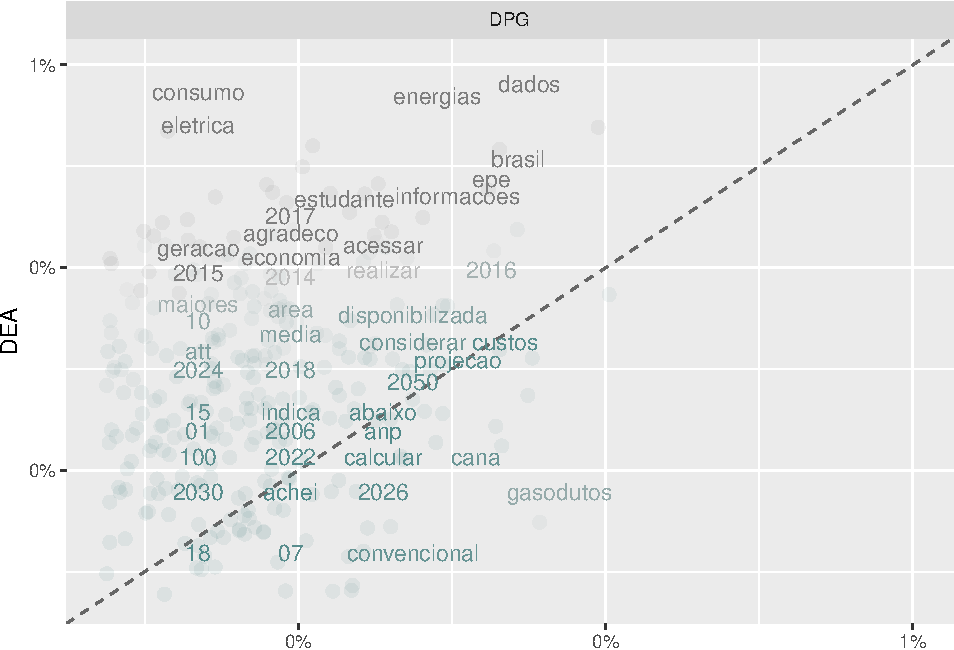
\includegraphics{markdown_v24_files/figure-latex/unnamed-chunk-59-1.pdf}

\begin{Shaded}
\begin{Highlighting}[]
\FunctionTok{Warning messages:}
\FunctionTok{1:}\AttributeTok{ Removed 4221 rows containing missing values (geom_point). }
\FunctionTok{2:}\AttributeTok{ Removed 4222 rows containing missing values (geom_text).}
\end{Highlighting}
\end{Shaded}

\begin{Shaded}
\begin{Highlighting}[]
\KeywordTok{cor.test}\NormalTok{(}\DataTypeTok{data =}\NormalTok{ freq04[freq04}\OperatorTok{$}\NormalTok{DIRETORIA }\OperatorTok{==}\StringTok{ "DPG"}\NormalTok{,],}
             \OperatorTok{~}\StringTok{ }\NormalTok{proportion }\OperatorTok{+}\StringTok{ `}\DataTypeTok{DEA}\StringTok{`}\NormalTok{)}
\end{Highlighting}
\end{Shaded}

\begin{verbatim}
## 
##  Pearson's product-moment correlation
## 
## data:  proportion and DEA
## t = 6.1072, df = 276, p-value = 3.432e-09
## alternative hypothesis: true correlation is not equal to 0
## 95 percent confidence interval:
##  0.2370151 0.4446322
## sample estimates:
##       cor 
## 0.3450374
\end{verbatim}

\begin{itemize}
\tightlist
\item
  DEA X DGC
\end{itemize}

\begin{Shaded}
\begin{Highlighting}[]
\NormalTok{freq05 <-}\StringTok{ }\NormalTok{PROP_PALAVRA }\OperatorTok
\StringTok{    }\KeywordTok{gather}\NormalTok{(DIRETORIA, proportion, }\KeywordTok{c}\NormalTok{(}\StringTok{`}\DataTypeTok{DGC}\StringTok{`}\NormalTok{))}
  
  \KeywordTok{library}\NormalTok{(scales)}
  \CommentTok{# expect a warning about rows with missing values being removed}
  \KeywordTok{ggplot}\NormalTok{(freq05, }\KeywordTok{aes}\NormalTok{(}\DataTypeTok{x =}\NormalTok{ proportion, }\DataTypeTok{y =} \StringTok{`}\DataTypeTok{DEA}\StringTok{`}\NormalTok{,}
                        \DataTypeTok{color =} \KeywordTok{abs}\NormalTok{(}\StringTok{`}\DataTypeTok{DEA}\StringTok{`} \OperatorTok{-}\StringTok{ }\NormalTok{proportion))) }\OperatorTok{+}
\StringTok{    }\KeywordTok{geom_abline}\NormalTok{(}\DataTypeTok{color =} \StringTok{"gray40"}\NormalTok{, }\DataTypeTok{lty =} \DecValTok{2}\NormalTok{) }\OperatorTok{+}
\StringTok{    }\KeywordTok{geom_jitter}\NormalTok{(}\DataTypeTok{alpha =} \FloatTok{0.1}\NormalTok{, }\DataTypeTok{size =} \FloatTok{2.5}\NormalTok{, }\DataTypeTok{width =} \FloatTok{0.3}\NormalTok{, }\DataTypeTok{height =} \FloatTok{0.3}\NormalTok{) }\OperatorTok{+}
\StringTok{    }\KeywordTok{geom_text}\NormalTok{(}\KeywordTok{aes}\NormalTok{(}\DataTypeTok{label =}\NormalTok{ palavra), }\DataTypeTok{check_overlap =} \OtherTok{TRUE}\NormalTok{, }\DataTypeTok{vjust =} \FloatTok{1.5}\NormalTok{) }\OperatorTok{+}
\StringTok{    }\KeywordTok{scale_x_log10}\NormalTok{(}\DataTypeTok{labels =} \KeywordTok{percent_format}\NormalTok{(}\DataTypeTok{big.mark =} \StringTok{"."}\NormalTok{, }\DataTypeTok{decimal.mark =} \StringTok{","}\NormalTok{, }\DataTypeTok{accuracy =} \DecValTok{1}\NormalTok{), }\DataTypeTok{limits =} \KeywordTok{c}\NormalTok{(}\OtherTok{NA}\NormalTok{, }\FloatTok{0.01}\NormalTok{)) }\OperatorTok{+}
\StringTok{    }\KeywordTok{scale_y_log10}\NormalTok{(}\DataTypeTok{labels =} \KeywordTok{percent_format}\NormalTok{(}\DataTypeTok{big.mark =} \StringTok{"."}\NormalTok{, }\DataTypeTok{decimal.mark =} \StringTok{","}\NormalTok{, }\DataTypeTok{accuracy =} \DecValTok{1}\NormalTok{), }\DataTypeTok{limits =} \KeywordTok{c}\NormalTok{(}\OtherTok{NA}\NormalTok{, }\FloatTok{0.01}\NormalTok{)) }\OperatorTok{+}
\StringTok{    }\KeywordTok{scale_color_gradient}\NormalTok{(}\DataTypeTok{limits =} \KeywordTok{c}\NormalTok{(}\DecValTok{0}\NormalTok{, }\FloatTok{0.001}\NormalTok{),}
                         \DataTypeTok{low =} \StringTok{"darkslategray4"}\NormalTok{, }\DataTypeTok{high =} \StringTok{"gray75"}\NormalTok{) }\OperatorTok{+}
\StringTok{    }\KeywordTok{facet_wrap}\NormalTok{(}\OperatorTok{~}\NormalTok{DIRETORIA, }\DataTypeTok{ncol =} \DecValTok{1}\NormalTok{) }\OperatorTok{+}
\StringTok{    }\KeywordTok{theme}\NormalTok{(}\DataTypeTok{legend.position=}\StringTok{"none"}\NormalTok{) }\OperatorTok{+}
\StringTok{    }\KeywordTok{labs}\NormalTok{(}\DataTypeTok{y =} \StringTok{"DEA"}\NormalTok{, }\DataTypeTok{x =} \OtherTok{NULL}\NormalTok{)}
\end{Highlighting}
\end{Shaded}

\begin{verbatim}
## Warning: Removed 3088 rows containing missing values (geom_point).
\end{verbatim}

\begin{verbatim}
## Warning: Removed 3086 rows containing missing values (geom_text).
\end{verbatim}

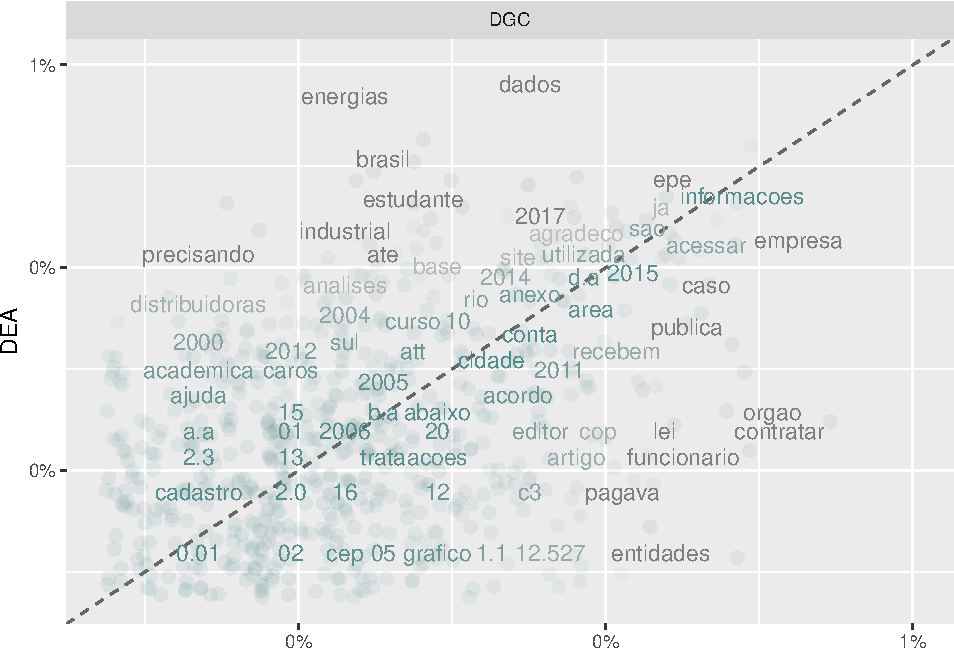
\includegraphics{markdown_v24_files/figure-latex/unnamed-chunk-61-1.pdf}

\begin{Shaded}
\begin{Highlighting}[]
\FunctionTok{Warning messages:}
\FunctionTok{1:}\AttributeTok{ Removed 3812 rows containing missing values (geom_point). }
\FunctionTok{2:}\AttributeTok{ Removed 3813 rows containing missing values (geom_text).}
\end{Highlighting}
\end{Shaded}

\begin{Shaded}
\begin{Highlighting}[]
\KeywordTok{cor.test}\NormalTok{(}\DataTypeTok{data =}\NormalTok{ freq05[freq05}\OperatorTok{$}\NormalTok{DIRETORIA }\OperatorTok{==}\StringTok{ "DGC"}\NormalTok{,],}
             \OperatorTok{~}\StringTok{ }\NormalTok{proportion }\OperatorTok{+}\StringTok{ `}\DataTypeTok{DEA}\StringTok{`}\NormalTok{)}
\end{Highlighting}
\end{Shaded}

\begin{verbatim}
## 
##  Pearson's product-moment correlation
## 
## data:  proportion and DEA
## t = 7.5906, df = 627, p-value = 1.158e-13
## alternative hypothesis: true correlation is not equal to 0
## 95 percent confidence interval:
##  0.2168448 0.3601121
## sample estimates:
##      cor 
## 0.290103
\end{verbatim}

\begin{itemize}
\tightlist
\item
  DEA X OUTROS
\end{itemize}

\begin{Shaded}
\begin{Highlighting}[]
\NormalTok{freq06 <-}\StringTok{ }\NormalTok{PROP_PALAVRA }\OperatorTok
\StringTok{    }\KeywordTok{gather}\NormalTok{(DIRETORIA, proportion, }\KeywordTok{c}\NormalTok{(}\StringTok{`}\DataTypeTok{OUTROS}\StringTok{`}\NormalTok{))}
  
  \KeywordTok{library}\NormalTok{(scales)}
  \CommentTok{# expect a warning about rows with missing values being removed}
  \KeywordTok{ggplot}\NormalTok{(freq06, }\KeywordTok{aes}\NormalTok{(}\DataTypeTok{x =}\NormalTok{ proportion, }\DataTypeTok{y =} \StringTok{`}\DataTypeTok{DEA}\StringTok{`}\NormalTok{,}
                        \DataTypeTok{color =} \KeywordTok{abs}\NormalTok{(}\StringTok{`}\DataTypeTok{DEA}\StringTok{`} \OperatorTok{-}\StringTok{ }\NormalTok{proportion))) }\OperatorTok{+}
\StringTok{    }\KeywordTok{geom_abline}\NormalTok{(}\DataTypeTok{color =} \StringTok{"gray40"}\NormalTok{, }\DataTypeTok{lty =} \DecValTok{2}\NormalTok{) }\OperatorTok{+}
\StringTok{    }\KeywordTok{geom_jitter}\NormalTok{(}\DataTypeTok{alpha =} \FloatTok{0.1}\NormalTok{, }\DataTypeTok{size =} \FloatTok{2.5}\NormalTok{, }\DataTypeTok{width =} \FloatTok{0.3}\NormalTok{, }\DataTypeTok{height =} \FloatTok{0.3}\NormalTok{) }\OperatorTok{+}
\StringTok{    }\KeywordTok{geom_text}\NormalTok{(}\KeywordTok{aes}\NormalTok{(}\DataTypeTok{label =}\NormalTok{ palavra), }\DataTypeTok{check_overlap =} \OtherTok{TRUE}\NormalTok{, }\DataTypeTok{vjust =} \FloatTok{1.5}\NormalTok{) }\OperatorTok{+}
\StringTok{    }\KeywordTok{scale_x_log10}\NormalTok{(}\DataTypeTok{labels =} \KeywordTok{percent_format}\NormalTok{(}\DataTypeTok{big.mark =} \StringTok{"."}\NormalTok{, }\DataTypeTok{decimal.mark =} \StringTok{","}\NormalTok{, }\DataTypeTok{accuracy =} \DecValTok{1}\NormalTok{), }\DataTypeTok{limits =} \KeywordTok{c}\NormalTok{(}\OtherTok{NA}\NormalTok{, }\FloatTok{0.01}\NormalTok{)) }\OperatorTok{+}
\StringTok{    }\KeywordTok{scale_y_log10}\NormalTok{(}\DataTypeTok{labels =} \KeywordTok{percent_format}\NormalTok{(}\DataTypeTok{big.mark =} \StringTok{"."}\NormalTok{, }\DataTypeTok{decimal.mark =} \StringTok{","}\NormalTok{, }\DataTypeTok{accuracy =} \DecValTok{1}\NormalTok{), }\DataTypeTok{limits =} \KeywordTok{c}\NormalTok{(}\OtherTok{NA}\NormalTok{, }\FloatTok{0.01}\NormalTok{)) }\OperatorTok{+}
\StringTok{    }\KeywordTok{scale_color_gradient}\NormalTok{(}\DataTypeTok{limits =} \KeywordTok{c}\NormalTok{(}\DecValTok{0}\NormalTok{, }\FloatTok{0.001}\NormalTok{),}
                         \DataTypeTok{low =} \StringTok{"darkslategray4"}\NormalTok{, }\DataTypeTok{high =} \StringTok{"gray75"}\NormalTok{) }\OperatorTok{+}
\StringTok{    }\KeywordTok{facet_wrap}\NormalTok{(}\OperatorTok{~}\NormalTok{DIRETORIA, }\DataTypeTok{ncol =} \DecValTok{1}\NormalTok{) }\OperatorTok{+}
\StringTok{    }\KeywordTok{theme}\NormalTok{(}\DataTypeTok{legend.position=}\StringTok{"none"}\NormalTok{) }\OperatorTok{+}
\StringTok{    }\KeywordTok{labs}\NormalTok{(}\DataTypeTok{y =} \StringTok{"DEA"}\NormalTok{, }\DataTypeTok{x =} \OtherTok{NULL}\NormalTok{)}
\end{Highlighting}
\end{Shaded}

\begin{verbatim}
## Warning: Removed 3499 rows containing missing values (geom_point).
\end{verbatim}

\begin{verbatim}
## Warning: Removed 3498 rows containing missing values (geom_text).
\end{verbatim}

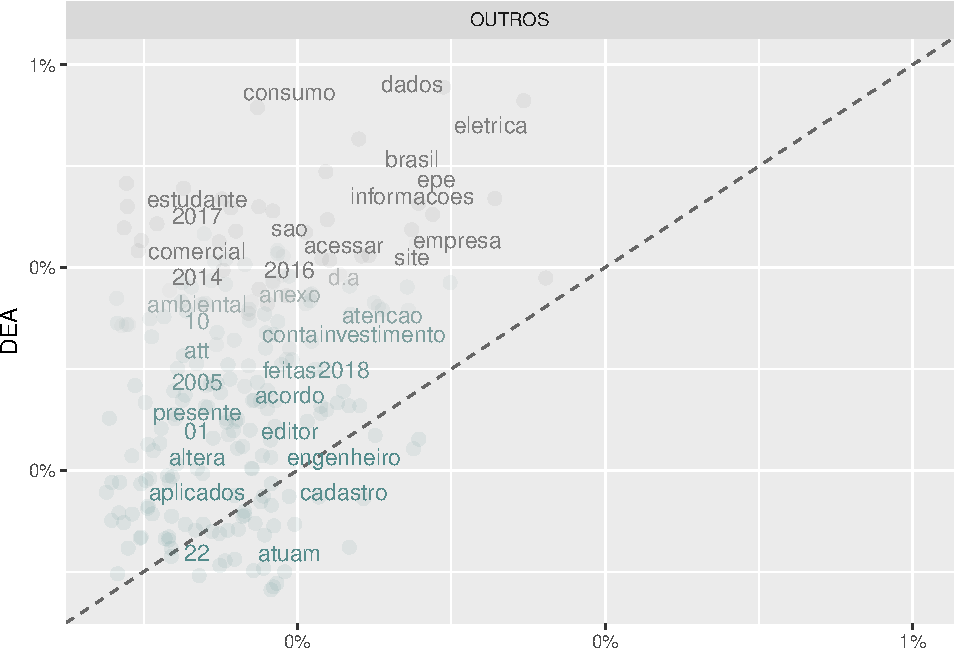
\includegraphics{markdown_v24_files/figure-latex/unnamed-chunk-63-1.pdf}

\begin{Shaded}
\begin{Highlighting}[]
\FunctionTok{Warning messages:}
\FunctionTok{1:}\AttributeTok{ Removed 4303 rows containing missing values (geom_point). }
\FunctionTok{2:}\AttributeTok{ Removed 4304 rows containing missing values (geom_text). }
\end{Highlighting}
\end{Shaded}

\begin{Shaded}
\begin{Highlighting}[]
\KeywordTok{cor.test}\NormalTok{(}\DataTypeTok{data =}\NormalTok{ freq06[freq06}\OperatorTok{$}\NormalTok{DIRETORIA }\OperatorTok{==}\StringTok{ "OUTROS"}\NormalTok{,],}
             \OperatorTok{~}\StringTok{ }\NormalTok{proportion }\OperatorTok{+}\StringTok{ `}\DataTypeTok{DEA}\StringTok{`}\NormalTok{)}
\end{Highlighting}
\end{Shaded}

\begin{verbatim}
## 
##  Pearson's product-moment correlation
## 
## data:  proportion and DEA
## t = 10.187, df = 215, p-value < 2.2e-16
## alternative hypothesis: true correlation is not equal to 0
## 95 percent confidence interval:
##  0.4733414 0.6540412
## sample estimates:
##       cor 
## 0.5705569
\end{verbatim}

\begin{itemize}
\tightlist
\item
  DPG X DGC
\end{itemize}

\begin{Shaded}
\begin{Highlighting}[]
\NormalTok{freq07 <-}\StringTok{ }\NormalTok{PROP_PALAVRA }\OperatorTok
\StringTok{    }\KeywordTok{gather}\NormalTok{(DIRETORIA, proportion, }\KeywordTok{c}\NormalTok{(}\StringTok{`}\DataTypeTok{DGC}\StringTok{`}\NormalTok{))}
  
  \KeywordTok{library}\NormalTok{(scales)}
  \CommentTok{# expect a warning about rows with missing values being removed}
  \KeywordTok{ggplot}\NormalTok{(freq07, }\KeywordTok{aes}\NormalTok{(}\DataTypeTok{x =}\NormalTok{ proportion, }\DataTypeTok{y =} \StringTok{`}\DataTypeTok{DPG}\StringTok{`}\NormalTok{,}
                        \DataTypeTok{color =} \KeywordTok{abs}\NormalTok{(}\StringTok{`}\DataTypeTok{DPG}\StringTok{`} \OperatorTok{-}\StringTok{ }\NormalTok{proportion))) }\OperatorTok{+}
\StringTok{    }\KeywordTok{geom_abline}\NormalTok{(}\DataTypeTok{color =} \StringTok{"gray40"}\NormalTok{, }\DataTypeTok{lty =} \DecValTok{2}\NormalTok{) }\OperatorTok{+}
\StringTok{    }\KeywordTok{geom_jitter}\NormalTok{(}\DataTypeTok{alpha =} \FloatTok{0.1}\NormalTok{, }\DataTypeTok{size =} \FloatTok{2.5}\NormalTok{, }\DataTypeTok{width =} \FloatTok{0.3}\NormalTok{, }\DataTypeTok{height =} \FloatTok{0.3}\NormalTok{) }\OperatorTok{+}
\StringTok{    }\KeywordTok{geom_text}\NormalTok{(}\KeywordTok{aes}\NormalTok{(}\DataTypeTok{label =}\NormalTok{ palavra), }\DataTypeTok{check_overlap =} \OtherTok{TRUE}\NormalTok{, }\DataTypeTok{vjust =} \FloatTok{1.5}\NormalTok{) }\OperatorTok{+}
\StringTok{    }\KeywordTok{scale_x_log10}\NormalTok{(}\DataTypeTok{labels =} \KeywordTok{percent_format}\NormalTok{(}\DataTypeTok{big.mark =} \StringTok{"."}\NormalTok{, }\DataTypeTok{decimal.mark =} \StringTok{","}\NormalTok{, }\DataTypeTok{accuracy =} \DecValTok{1}\NormalTok{), }\DataTypeTok{limits =} \KeywordTok{c}\NormalTok{(}\OtherTok{NA}\NormalTok{, }\FloatTok{0.01}\NormalTok{)) }\OperatorTok{+}
\StringTok{    }\KeywordTok{scale_y_log10}\NormalTok{(}\DataTypeTok{labels =} \KeywordTok{percent_format}\NormalTok{(}\DataTypeTok{big.mark =} \StringTok{"."}\NormalTok{, }\DataTypeTok{decimal.mark =} \StringTok{","}\NormalTok{, }\DataTypeTok{accuracy =} \DecValTok{1}\NormalTok{), }\DataTypeTok{limits =} \KeywordTok{c}\NormalTok{(}\OtherTok{NA}\NormalTok{, }\FloatTok{0.01}\NormalTok{)) }\OperatorTok{+}
\StringTok{    }\KeywordTok{scale_color_gradient}\NormalTok{(}\DataTypeTok{limits =} \KeywordTok{c}\NormalTok{(}\DecValTok{0}\NormalTok{, }\FloatTok{0.001}\NormalTok{),}
                         \DataTypeTok{low =} \StringTok{"darkslategray4"}\NormalTok{, }\DataTypeTok{high =} \StringTok{"gray75"}\NormalTok{) }\OperatorTok{+}
\StringTok{    }\KeywordTok{facet_wrap}\NormalTok{(}\OperatorTok{~}\NormalTok{DIRETORIA, }\DataTypeTok{ncol =} \DecValTok{1}\NormalTok{) }\OperatorTok{+}
\StringTok{    }\KeywordTok{theme}\NormalTok{(}\DataTypeTok{legend.position=}\StringTok{"none"}\NormalTok{) }\OperatorTok{+}
\StringTok{    }\KeywordTok{labs}\NormalTok{(}\DataTypeTok{y =} \StringTok{"DPG"}\NormalTok{, }\DataTypeTok{x =} \OtherTok{NULL}\NormalTok{)}
\end{Highlighting}
\end{Shaded}

\begin{verbatim}
## Warning: Removed 3507 rows containing missing values (geom_point).
\end{verbatim}

\begin{verbatim}
## Warning: Removed 3507 rows containing missing values (geom_text).
\end{verbatim}

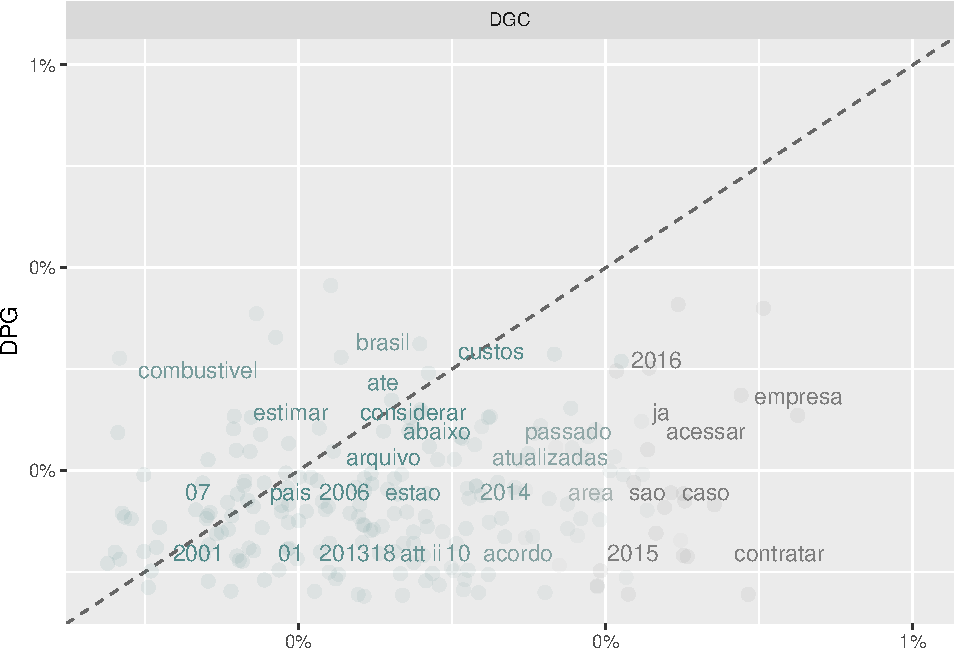
\includegraphics{markdown_v24_files/figure-latex/unnamed-chunk-65-1.pdf}

\begin{Shaded}
\begin{Highlighting}[]
\FunctionTok{Warning messages:}
\FunctionTok{1:}\AttributeTok{ Removed 4296 rows containing missing values (geom_point). }
\FunctionTok{2:}\AttributeTok{ Removed 4297 rows containing missing values (geom_text). }
\end{Highlighting}
\end{Shaded}

\begin{Shaded}
\begin{Highlighting}[]
\KeywordTok{cor.test}\NormalTok{(}\DataTypeTok{data =}\NormalTok{ freq07[freq07}\OperatorTok{$}\NormalTok{DIRETORIA }\OperatorTok{==}\StringTok{ "DGC"}\NormalTok{,],}
             \OperatorTok{~}\StringTok{ }\NormalTok{proportion }\OperatorTok{+}\StringTok{ `}\DataTypeTok{DPG}\StringTok{`}\NormalTok{)}
\end{Highlighting}
\end{Shaded}

\begin{verbatim}
## 
##  Pearson's product-moment correlation
## 
## data:  proportion and DPG
## t = 3.4202, df = 206, p-value = 0.0007543
## alternative hypothesis: true correlation is not equal to 0
## 95 percent confidence interval:
##  0.09888554 0.35660374
## sample estimates:
##       cor 
## 0.2318083
\end{verbatim}

\begin{itemize}
\tightlist
\item
  DPG X OUTROS
\end{itemize}

\begin{Shaded}
\begin{Highlighting}[]
\NormalTok{freq08 <-}\StringTok{ }\NormalTok{PROP_PALAVRA }\OperatorTok
\StringTok{    }\KeywordTok{gather}\NormalTok{(DIRETORIA, proportion, }\KeywordTok{c}\NormalTok{(}\StringTok{`}\DataTypeTok{OUTROS}\StringTok{`}\NormalTok{))}
  
  \KeywordTok{library}\NormalTok{(scales)}
  \CommentTok{# expect a warning about rows with missing values being removed}
  \KeywordTok{ggplot}\NormalTok{(freq08, }\KeywordTok{aes}\NormalTok{(}\DataTypeTok{x =}\NormalTok{ proportion, }\DataTypeTok{y =} \StringTok{`}\DataTypeTok{DPG}\StringTok{`}\NormalTok{,}
                        \DataTypeTok{color =} \KeywordTok{abs}\NormalTok{(}\StringTok{`}\DataTypeTok{DPG}\StringTok{`} \OperatorTok{-}\StringTok{ }\NormalTok{proportion))) }\OperatorTok{+}
\StringTok{    }\KeywordTok{geom_abline}\NormalTok{(}\DataTypeTok{color =} \StringTok{"gray40"}\NormalTok{, }\DataTypeTok{lty =} \DecValTok{2}\NormalTok{) }\OperatorTok{+}
\StringTok{    }\KeywordTok{geom_jitter}\NormalTok{(}\DataTypeTok{alpha =} \FloatTok{0.1}\NormalTok{, }\DataTypeTok{size =} \FloatTok{2.5}\NormalTok{, }\DataTypeTok{width =} \FloatTok{0.3}\NormalTok{, }\DataTypeTok{height =} \FloatTok{0.3}\NormalTok{) }\OperatorTok{+}
\StringTok{    }\KeywordTok{geom_text}\NormalTok{(}\KeywordTok{aes}\NormalTok{(}\DataTypeTok{label =}\NormalTok{ palavra), }\DataTypeTok{check_overlap =} \OtherTok{TRUE}\NormalTok{, }\DataTypeTok{vjust =} \FloatTok{1.5}\NormalTok{) }\OperatorTok{+}
\StringTok{    }\KeywordTok{scale_x_log10}\NormalTok{(}\DataTypeTok{labels =} \KeywordTok{percent_format}\NormalTok{(}\DataTypeTok{big.mark =} \StringTok{"."}\NormalTok{, }\DataTypeTok{decimal.mark =} \StringTok{","}\NormalTok{, }\DataTypeTok{accuracy =} \DecValTok{1}\NormalTok{), }\DataTypeTok{limits =} \KeywordTok{c}\NormalTok{(}\OtherTok{NA}\NormalTok{, }\FloatTok{0.01}\NormalTok{)) }\OperatorTok{+}
\StringTok{    }\KeywordTok{scale_y_log10}\NormalTok{(}\DataTypeTok{labels =} \KeywordTok{percent_format}\NormalTok{(}\DataTypeTok{big.mark =} \StringTok{"."}\NormalTok{, }\DataTypeTok{decimal.mark =} \StringTok{","}\NormalTok{, }\DataTypeTok{accuracy =} \DecValTok{1}\NormalTok{), }\DataTypeTok{limits =} \KeywordTok{c}\NormalTok{(}\OtherTok{NA}\NormalTok{, }\FloatTok{0.01}\NormalTok{)) }\OperatorTok{+}
\StringTok{    }\KeywordTok{scale_color_gradient}\NormalTok{(}\DataTypeTok{limits =} \KeywordTok{c}\NormalTok{(}\DecValTok{0}\NormalTok{, }\FloatTok{0.001}\NormalTok{),}
                         \DataTypeTok{low =} \StringTok{"darkslategray4"}\NormalTok{, }\DataTypeTok{high =} \StringTok{"gray75"}\NormalTok{) }\OperatorTok{+}
\StringTok{    }\KeywordTok{facet_wrap}\NormalTok{(}\OperatorTok{~}\NormalTok{DIRETORIA, }\DataTypeTok{ncol =} \DecValTok{1}\NormalTok{) }\OperatorTok{+}
\StringTok{    }\KeywordTok{theme}\NormalTok{(}\DataTypeTok{legend.position=}\StringTok{"none"}\NormalTok{) }\OperatorTok{+}
\StringTok{    }\KeywordTok{labs}\NormalTok{(}\DataTypeTok{y =} \StringTok{"DPG"}\NormalTok{, }\DataTypeTok{x =} \OtherTok{NULL}\NormalTok{)}
\end{Highlighting}
\end{Shaded}

\begin{verbatim}
## Warning: Removed 3623 rows containing missing values (geom_point).
\end{verbatim}

\begin{verbatim}
## Warning: Removed 3623 rows containing missing values (geom_text).
\end{verbatim}

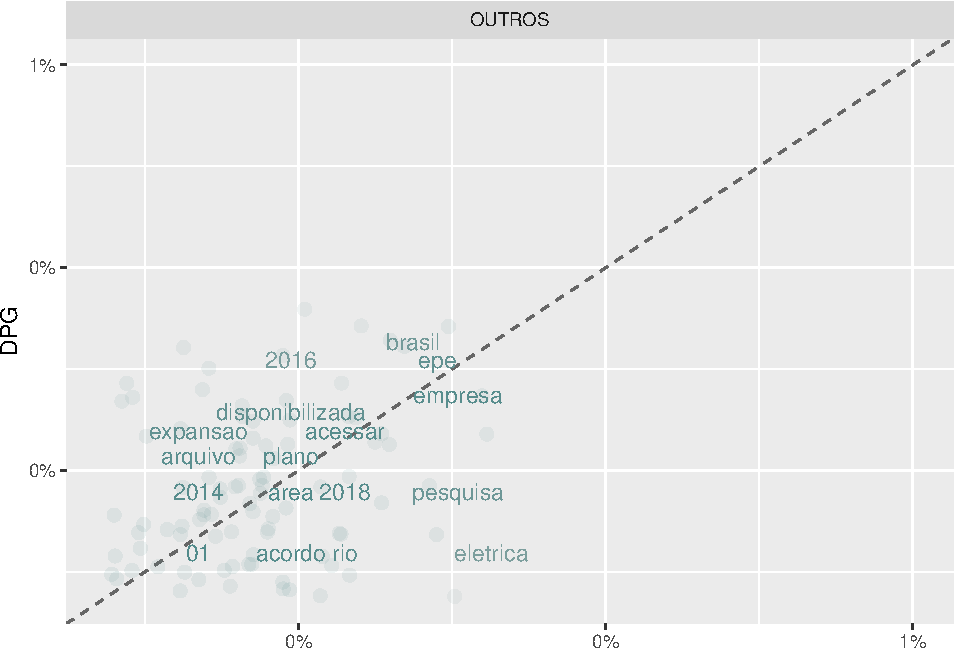
\includegraphics{markdown_v24_files/figure-latex/unnamed-chunk-67-1.pdf}

\begin{Shaded}
\begin{Highlighting}[]
\FunctionTok{Warning messages:}
\FunctionTok{1:}\AttributeTok{ Removed 4450 rows containing missing values (geom_point). }
\FunctionTok{2:}\AttributeTok{ Removed 4451 rows containing missing values (geom_text). }
\end{Highlighting}
\end{Shaded}

\begin{Shaded}
\begin{Highlighting}[]
\KeywordTok{cor.test}\NormalTok{(}\DataTypeTok{data =}\NormalTok{ freq08[freq08}\OperatorTok{$}\NormalTok{DIRETORIA }\OperatorTok{==}\StringTok{ "OUTROS"}\NormalTok{,],}
             \OperatorTok{~}\StringTok{ }\NormalTok{proportion }\OperatorTok{+}\StringTok{ `}\DataTypeTok{DPG}\StringTok{`}\NormalTok{)}
\end{Highlighting}
\end{Shaded}

\begin{verbatim}
## 
##  Pearson's product-moment correlation
## 
## data:  proportion and DPG
## t = 5.0342, df = 90, p-value = 2.447e-06
## alternative hypothesis: true correlation is not equal to 0
## 95 percent confidence interval:
##  0.2919524 0.6145567
## sample estimates:
##       cor 
## 0.4687405
\end{verbatim}

\begin{itemize}
\tightlist
\item
  DGC X OUTROS
\end{itemize}

\begin{Shaded}
\begin{Highlighting}[]
\NormalTok{freq09 <-}\StringTok{ }\NormalTok{PROP_PALAVRA }\OperatorTok
\StringTok{    }\KeywordTok{gather}\NormalTok{(DIRETORIA, proportion, }\KeywordTok{c}\NormalTok{(}\StringTok{`}\DataTypeTok{OUTROS}\StringTok{`}\NormalTok{))}
  
  \KeywordTok{library}\NormalTok{(scales)}
  \CommentTok{# expect a warning about rows with missing values being removed}
  \KeywordTok{ggplot}\NormalTok{(freq08, }\KeywordTok{aes}\NormalTok{(}\DataTypeTok{x =}\NormalTok{ proportion, }\DataTypeTok{y =} \StringTok{`}\DataTypeTok{DGC}\StringTok{`}\NormalTok{,}
                        \DataTypeTok{color =} \KeywordTok{abs}\NormalTok{(}\StringTok{`}\DataTypeTok{DGC}\StringTok{`} \OperatorTok{-}\StringTok{ }\NormalTok{proportion))) }\OperatorTok{+}
\StringTok{    }\KeywordTok{geom_abline}\NormalTok{(}\DataTypeTok{color =} \StringTok{"gray40"}\NormalTok{, }\DataTypeTok{lty =} \DecValTok{2}\NormalTok{) }\OperatorTok{+}
\StringTok{    }\KeywordTok{geom_jitter}\NormalTok{(}\DataTypeTok{alpha =} \FloatTok{0.1}\NormalTok{, }\DataTypeTok{size =} \FloatTok{2.5}\NormalTok{, }\DataTypeTok{width =} \FloatTok{0.3}\NormalTok{, }\DataTypeTok{height =} \FloatTok{0.3}\NormalTok{) }\OperatorTok{+}
\StringTok{    }\KeywordTok{geom_text}\NormalTok{(}\KeywordTok{aes}\NormalTok{(}\DataTypeTok{label =}\NormalTok{ palavra), }\DataTypeTok{check_overlap =} \OtherTok{TRUE}\NormalTok{, }\DataTypeTok{vjust =} \FloatTok{1.5}\NormalTok{) }\OperatorTok{+}
\StringTok{    }\KeywordTok{scale_x_log10}\NormalTok{(}\DataTypeTok{labels =} \KeywordTok{percent_format}\NormalTok{(}\DataTypeTok{big.mark =} \StringTok{"."}\NormalTok{, }\DataTypeTok{decimal.mark =} \StringTok{","}\NormalTok{, }\DataTypeTok{accuracy =} \DecValTok{1}\NormalTok{), }\DataTypeTok{limits =} \KeywordTok{c}\NormalTok{(}\OtherTok{NA}\NormalTok{, }\FloatTok{0.01}\NormalTok{)) }\OperatorTok{+}
\StringTok{    }\KeywordTok{scale_y_log10}\NormalTok{(}\DataTypeTok{labels =} \KeywordTok{percent_format}\NormalTok{(}\DataTypeTok{big.mark =} \StringTok{"."}\NormalTok{, }\DataTypeTok{decimal.mark =} \StringTok{","}\NormalTok{, }\DataTypeTok{accuracy =} \DecValTok{1}\NormalTok{), }\DataTypeTok{limits =} \KeywordTok{c}\NormalTok{(}\OtherTok{NA}\NormalTok{, }\FloatTok{0.01}\NormalTok{)) }\OperatorTok{+}
\StringTok{    }\KeywordTok{scale_color_gradient}\NormalTok{(}\DataTypeTok{limits =} \KeywordTok{c}\NormalTok{(}\DecValTok{0}\NormalTok{, }\FloatTok{0.001}\NormalTok{),}
                         \DataTypeTok{low =} \StringTok{"darkslategray4"}\NormalTok{, }\DataTypeTok{high =} \StringTok{"gray75"}\NormalTok{) }\OperatorTok{+}
\StringTok{    }\KeywordTok{facet_wrap}\NormalTok{(}\OperatorTok{~}\NormalTok{DIRETORIA, }\DataTypeTok{ncol =} \DecValTok{1}\NormalTok{) }\OperatorTok{+}
\StringTok{    }\KeywordTok{theme}\NormalTok{(}\DataTypeTok{legend.position=}\StringTok{"none"}\NormalTok{) }\OperatorTok{+}
\StringTok{    }\KeywordTok{labs}\NormalTok{(}\DataTypeTok{y =} \StringTok{"DGC"}\NormalTok{, }\DataTypeTok{x =} \OtherTok{NULL}\NormalTok{)}
\end{Highlighting}
\end{Shaded}

\begin{verbatim}
## Warning: Removed 3510 rows containing missing values (geom_point).
\end{verbatim}

\begin{verbatim}
## Warning: Removed 3510 rows containing missing values (geom_text).
\end{verbatim}

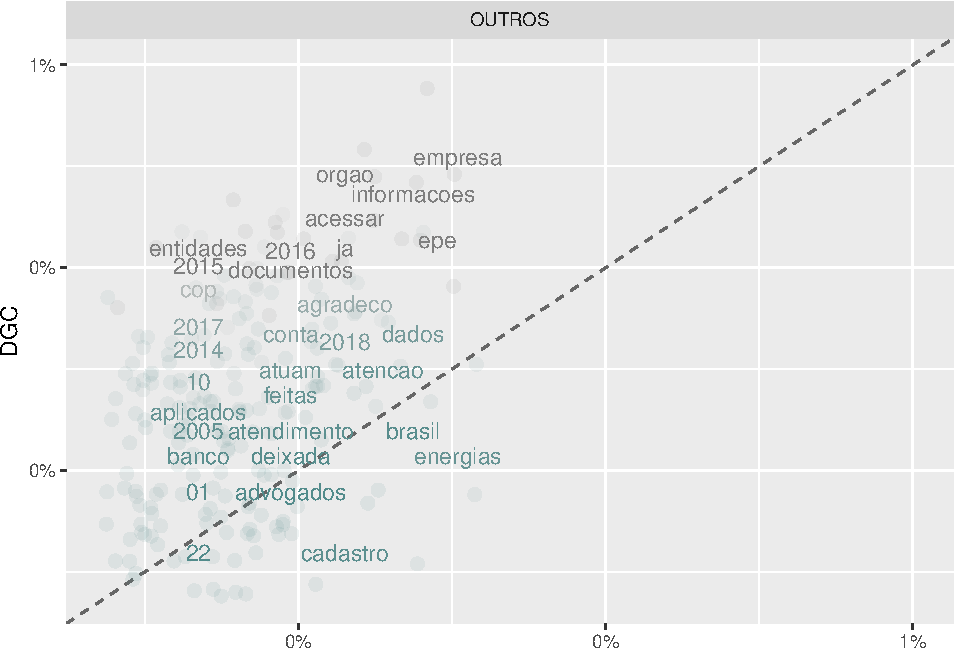
\includegraphics{markdown_v24_files/figure-latex/unnamed-chunk-69-1.pdf}

\begin{Shaded}
\begin{Highlighting}[]
\FunctionTok{Warning messages:}
\FunctionTok{1:}\AttributeTok{ Removed 4302 rows containing missing values (geom_point). }
\FunctionTok{2:}\AttributeTok{ Removed 4303 rows containing missing values (geom_text).}
\end{Highlighting}
\end{Shaded}

\begin{Shaded}
\begin{Highlighting}[]
\KeywordTok{cor.test}\NormalTok{(}\DataTypeTok{data =}\NormalTok{ freq09[freq09}\OperatorTok{$}\NormalTok{DIRETORIA }\OperatorTok{==}\StringTok{ "OUTROS"}\NormalTok{,],}
             \OperatorTok{~}\StringTok{ }\NormalTok{proportion }\OperatorTok{+}\StringTok{ `}\DataTypeTok{DGC}\StringTok{`}\NormalTok{)}
\end{Highlighting}
\end{Shaded}

\begin{verbatim}
## 
##  Pearson's product-moment correlation
## 
## data:  proportion and DGC
## t = 8.4142, df = 203, p-value = 7.03e-15
## alternative hypothesis: true correlation is not equal to 0
## 95 percent confidence interval:
##  0.3992974 0.6034898
## sample estimates:
##      cor 
## 0.508508
\end{verbatim}

\subsubsection{Usando bigram para n=2 palavras por
token}\label{usando-bigram-para-n2-palavras-por-token}

\paragraph{Frequência de palavras por
diretoria}\label{frequencia-de-palavras-por-diretoria-4}

\begin{Shaded}
\begin{Highlighting}[]
\NormalTok{diretoria_palavras_bigram <-}\StringTok{ }\NormalTok{DB }\OperatorTok
\StringTok{  }\KeywordTok{select}\NormalTok{(DESCRI_PEDIDO,DIRETORIA) }\OperatorTok
\StringTok{  }\KeywordTok{unnest_tokens}\NormalTok{(BIGRAM, DESCRI_PEDIDO, }\DataTypeTok{token =} \StringTok{"ngrams"}\NormalTok{, }\DataTypeTok{n =} \DecValTok{2}\NormalTok{) }\OperatorTok
\StringTok{  }\KeywordTok{count}\NormalTok{(DIRETORIA, BIGRAM, }\DataTypeTok{sort =} \OtherTok{TRUE}\NormalTok{) }\OperatorTok
\StringTok{  }\KeywordTok{ungroup}\NormalTok{()}
\CommentTok{#diretoria_palavras_bigram}

\NormalTok{plot_diretoria_palavras_bigram <-}\StringTok{ }\NormalTok{diretoria_palavras_bigram }\OperatorTok
\StringTok{  }\KeywordTok{bind_tf_idf}\NormalTok{(BIGRAM, DIRETORIA, n) }\OperatorTok
\StringTok{  }\KeywordTok{arrange}\NormalTok{(}\KeywordTok{desc}\NormalTok{(tf_idf)) }\OperatorTok
\StringTok{  }\KeywordTok{mutate}\NormalTok{(}\DataTypeTok{BIGRAM =} \KeywordTok{factor}\NormalTok{(BIGRAM, }\DataTypeTok{levels =} \KeywordTok{rev}\NormalTok{(}\KeywordTok{unique}\NormalTok{(BIGRAM)))) }\OperatorTok
\StringTok{  }\KeywordTok{mutate}\NormalTok{(}\DataTypeTok{DIRETORIA =} \KeywordTok{factor}\NormalTok{(DIRETORIA, }\DataTypeTok{levels =} \KeywordTok{c}\NormalTok{(}\StringTok{"DEA"}\NormalTok{,}
                                                  \StringTok{"DEE"}\NormalTok{,}
                                                  \StringTok{"DGC"}\NormalTok{,}
                                                  \StringTok{"DPG"}\NormalTok{,}
                                                  \StringTok{"OUTROS"}\NormalTok{)))}
\CommentTok{#View(head(plot_diretoria_palavras_bigram))}
\CommentTok{#jpeg("02_freq_palavras_dir.jpeg")}
\NormalTok{plot_diretoria_palavras_bigram }\OperatorTok
\KeywordTok{group_by}\NormalTok{(DIRETORIA) }\OperatorTok
\KeywordTok{top_n}\NormalTok{(}\DecValTok{10}\NormalTok{, tf_idf) }\OperatorTok
\KeywordTok{ungroup}\NormalTok{() }\OperatorTok
\KeywordTok{mutate}\NormalTok{(}\DataTypeTok{BIGRAM =} \KeywordTok{reorder}\NormalTok{(BIGRAM, tf_idf)) }\OperatorTok
\KeywordTok{ggplot}\NormalTok{(}\KeywordTok{aes}\NormalTok{(BIGRAM, tf_idf, }\DataTypeTok{fill =}\NormalTok{ DIRETORIA)) }\OperatorTok{+}
\KeywordTok{geom_col}\NormalTok{(}\DataTypeTok{show.legend =} \OtherTok{FALSE}\NormalTok{) }\OperatorTok{+}
\KeywordTok{labs}\NormalTok{(}\DataTypeTok{x =} \OtherTok{NULL}\NormalTok{, }\DataTypeTok{y =} \StringTok{"tf-idf"}\NormalTok{) }\OperatorTok{+}
\KeywordTok{facet_wrap}\NormalTok{(}\OperatorTok{~}\NormalTok{DIRETORIA, }\DataTypeTok{ncol =} \DecValTok{2}\NormalTok{, }\DataTypeTok{scales =} \StringTok{"free"}\NormalTok{) }\OperatorTok{+}
\KeywordTok{coord_flip}\NormalTok{() }\OperatorTok{+}\StringTok{ }
\KeywordTok{scale_y_continuous}\NormalTok{(}\DataTypeTok{labels=}\NormalTok{gcomma)}
\end{Highlighting}
\end{Shaded}

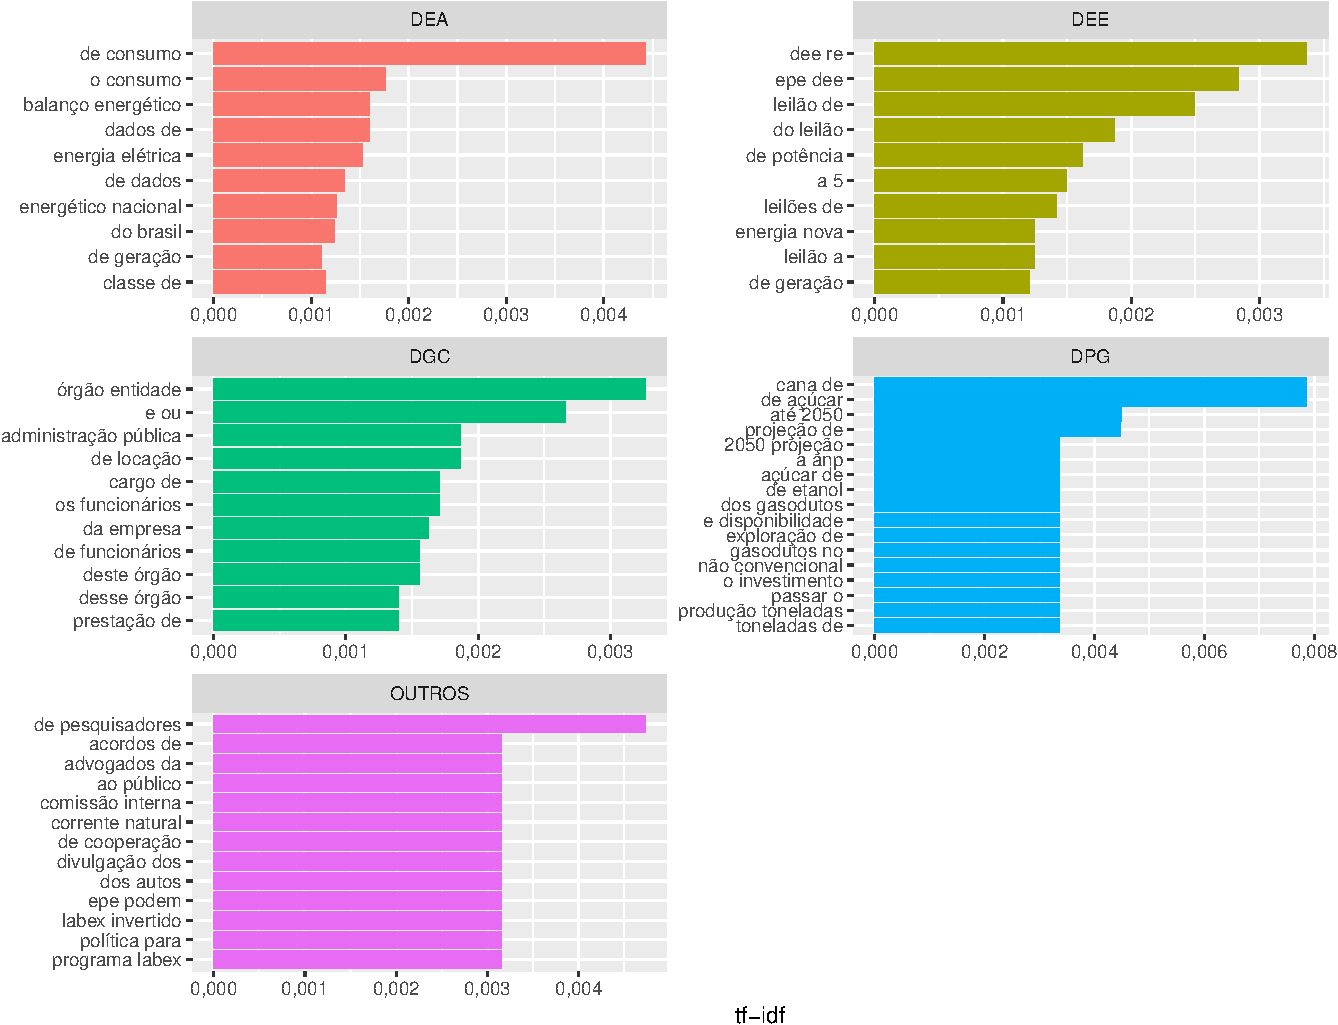
\includegraphics{markdown_v24_files/figure-latex/03_freq_palavras_dir-1.pdf}

\begin{Shaded}
\begin{Highlighting}[]
\CommentTok{#dev.off()}
\end{Highlighting}
\end{Shaded}

\subsubsection{Usando bigram para n=3 palavras por
token}\label{usando-bigram-para-n3-palavras-por-token}

\paragraph{Frequência de palavras por
diretoria}\label{frequencia-de-palavras-por-diretoria-5}

\begin{Shaded}
\begin{Highlighting}[]
\NormalTok{diretoria_palavras_trigram <-}\StringTok{ }\NormalTok{DB }\OperatorTok
\StringTok{  }\KeywordTok{select}\NormalTok{(DESCRI_PEDIDO,DIRETORIA) }\OperatorTok
\StringTok{  }\KeywordTok{unnest_tokens}\NormalTok{(TRIGRAM, DESCRI_PEDIDO, }\DataTypeTok{token =} \StringTok{"ngrams"}\NormalTok{, }\DataTypeTok{n =} \DecValTok{3}\NormalTok{) }\OperatorTok
\StringTok{  }\KeywordTok{count}\NormalTok{(DIRETORIA, TRIGRAM, }\DataTypeTok{sort =} \OtherTok{TRUE}\NormalTok{) }\OperatorTok
\StringTok{  }\KeywordTok{ungroup}\NormalTok{()}
\CommentTok{#diretoria_palavras_trigram}

\NormalTok{plot_diretoria_palavras_trigram <-}\StringTok{ }\NormalTok{diretoria_palavras_trigram }\OperatorTok
\StringTok{  }\KeywordTok{bind_tf_idf}\NormalTok{(TRIGRAM, DIRETORIA, n) }\OperatorTok
\StringTok{  }\KeywordTok{arrange}\NormalTok{(}\KeywordTok{desc}\NormalTok{(tf_idf)) }\OperatorTok
\StringTok{  }\KeywordTok{mutate}\NormalTok{(}\DataTypeTok{TRIGRAM =} \KeywordTok{factor}\NormalTok{(TRIGRAM, }\DataTypeTok{levels =} \KeywordTok{rev}\NormalTok{(}\KeywordTok{unique}\NormalTok{(TRIGRAM)))) }\OperatorTok
\StringTok{  }\KeywordTok{mutate}\NormalTok{(}\DataTypeTok{DIRETORIA =} \KeywordTok{factor}\NormalTok{(DIRETORIA, }\DataTypeTok{levels =} \KeywordTok{c}\NormalTok{(}\StringTok{"DEA"}\NormalTok{,}
                                                  \StringTok{"DEE"}\NormalTok{,}
                                                  \StringTok{"DGC"}\NormalTok{,}
                                                  \StringTok{"DPG"}\NormalTok{,}
                                                  \StringTok{"OUTROS"}\NormalTok{)))}
\CommentTok{#View(head(plot_diretoria_palavras_trigram))}
\CommentTok{#jpeg("02_freq_palavras_dir.jpeg")}
\NormalTok{plot_diretoria_palavras_trigram }\OperatorTok
\KeywordTok{group_by}\NormalTok{(DIRETORIA) }\OperatorTok
\KeywordTok{top_n}\NormalTok{(}\DecValTok{10}\NormalTok{, tf_idf) }\OperatorTok
\KeywordTok{ungroup}\NormalTok{() }\OperatorTok
\KeywordTok{mutate}\NormalTok{(}\DataTypeTok{TRIGRAM =} \KeywordTok{reorder}\NormalTok{(TRIGRAM, tf_idf)) }\OperatorTok
\KeywordTok{ggplot}\NormalTok{(}\KeywordTok{aes}\NormalTok{(TRIGRAM, tf_idf, }\DataTypeTok{fill =}\NormalTok{ DIRETORIA)) }\OperatorTok{+}
\KeywordTok{geom_col}\NormalTok{(}\DataTypeTok{show.legend =} \OtherTok{FALSE}\NormalTok{) }\OperatorTok{+}
\KeywordTok{labs}\NormalTok{(}\DataTypeTok{x =} \OtherTok{NULL}\NormalTok{, }\DataTypeTok{y =} \StringTok{"tf-idf"}\NormalTok{) }\OperatorTok{+}
\KeywordTok{facet_wrap}\NormalTok{(}\OperatorTok{~}\NormalTok{DIRETORIA, }\DataTypeTok{ncol =} \DecValTok{2}\NormalTok{, }\DataTypeTok{scales =} \StringTok{"free"}\NormalTok{) }\OperatorTok{+}
\KeywordTok{coord_flip}\NormalTok{() }\OperatorTok{+}\StringTok{ }
\KeywordTok{scale_y_continuous}\NormalTok{(}\DataTypeTok{labels=}\NormalTok{gcomma)}
\end{Highlighting}
\end{Shaded}

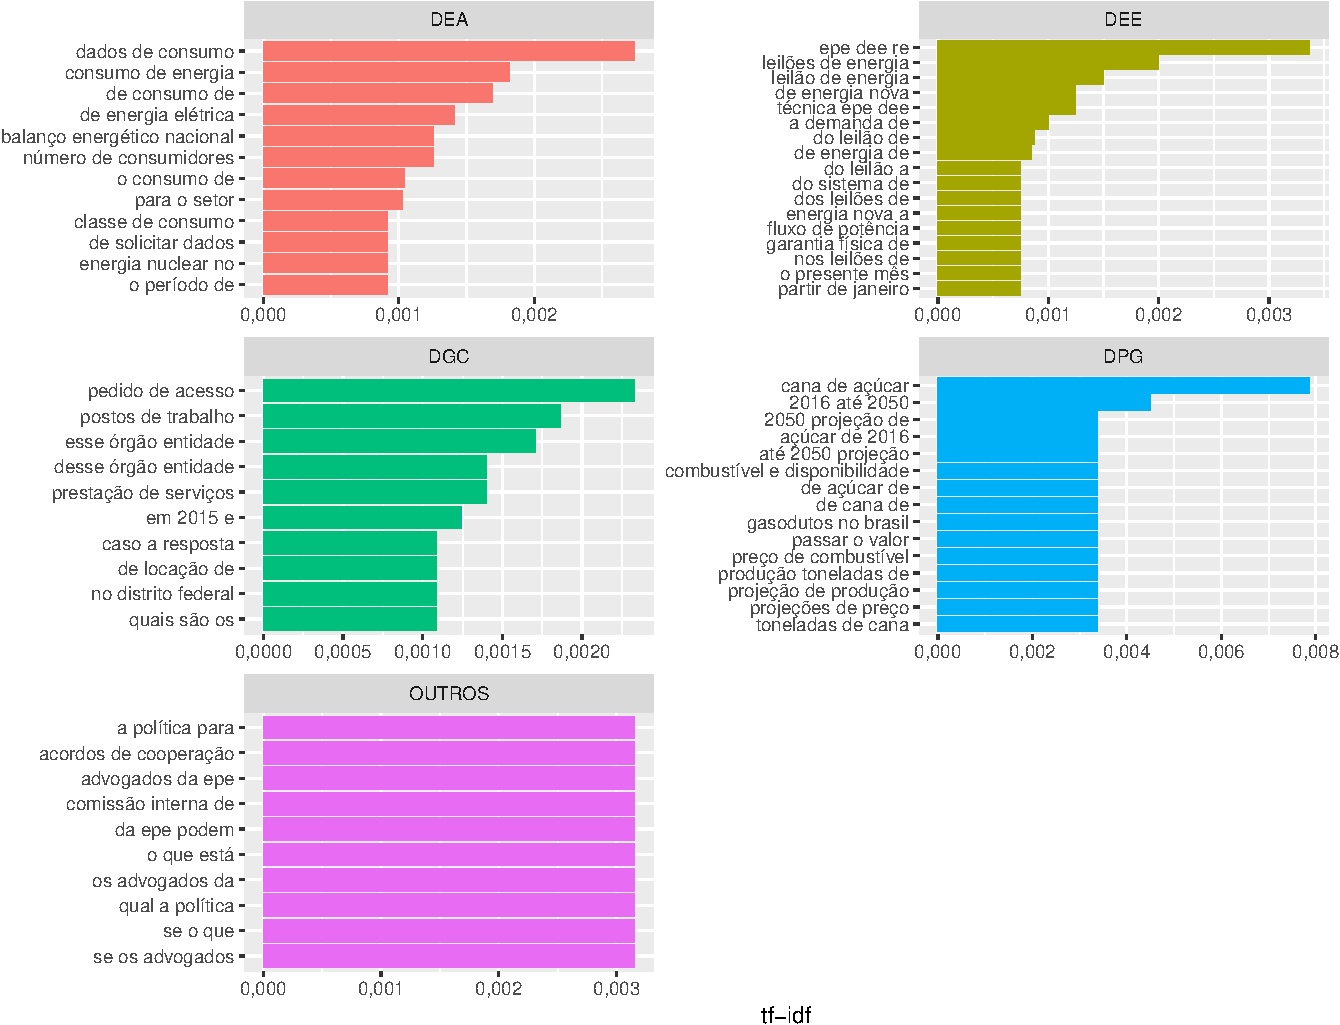
\includegraphics{markdown_v24_files/figure-latex/04_freq_palavras_dir-1.pdf}

\begin{Shaded}
\begin{Highlighting}[]
\CommentTok{#dev.off()}
\end{Highlighting}
\end{Shaded}

\subsection{tidy object into document-term
matrix}\label{tidy-object-into-document-term-matrix}

\begin{Shaded}
\begin{Highlighting}[]
\NormalTok{plot_diretoria_palavras <-}\StringTok{ }\NormalTok{diretoria_palavras }\OperatorTok
\StringTok{  }\KeywordTok{bind_tf_idf}\NormalTok{(palavra, DIRETORIA, n) }\OperatorTok
\StringTok{  }\KeywordTok{arrange}\NormalTok{(}\KeywordTok{desc}\NormalTok{(tf_idf)) }\OperatorTok
\StringTok{  }\KeywordTok{mutate}\NormalTok{(}\DataTypeTok{palavra =} \KeywordTok{factor}\NormalTok{(palavra, }\DataTypeTok{levels =} \KeywordTok{rev}\NormalTok{(}\KeywordTok{unique}\NormalTok{(palavra)))) }\OperatorTok
\StringTok{  }\KeywordTok{mutate}\NormalTok{(}\DataTypeTok{DIRETORIA =} \KeywordTok{factor}\NormalTok{(DIRETORIA, }\DataTypeTok{levels =} \KeywordTok{c}\NormalTok{(}\StringTok{"DEA"}\NormalTok{,}
                                                  \StringTok{"DEE"}\NormalTok{,}
                                                  \StringTok{"DGC"}\NormalTok{,}
                                                  \StringTok{"DPG"}\NormalTok{,}
                                                  \StringTok{"OUTROS"}\NormalTok{)))}

\NormalTok{dtm =}\StringTok{ }\NormalTok{plot_diretoria_palavras }\OperatorTok
\KeywordTok{cast_dtm}\NormalTok{(}\DataTypeTok{document =}\NormalTok{ DIRETORIA, }\DataTypeTok{term =}\NormalTok{ palavra, n)}
\end{Highlighting}
\end{Shaded}

\subsubsection{Nuvem de palavras}\label{nuvem-de-palavras}

\paragraph{Nuvem de palavras por diretoria - s/ steeming e/ c/ stopwords
-
onegram}\label{nuvem-de-palavras-por-diretoria---s-steeming-e-c-stopwords---onegram}

\begin{Shaded}
\begin{Highlighting}[]
\CommentTok{#View(head(plot_diretoria_palavras))}
\KeywordTok{library}\NormalTok{(wordcloud)}
\NormalTok{plot_diretorias_tf_dif =}\StringTok{ }\NormalTok{plot_diretoria_palavras }\OperatorTok
\StringTok{    }\KeywordTok{select}\NormalTok{(palavra, tf_idf, DIRETORIA) }\OperatorTok
\StringTok{    }\KeywordTok{mutate}\NormalTok{(}\DataTypeTok{palavra =} \KeywordTok{reorder}\NormalTok{(palavra, tf_idf))}

\NormalTok{## DEE}
\CommentTok{#jpeg("XX_wordclou_tfidf_dir01_DEE.jpeg")}
\NormalTok{nuvem1 =}\StringTok{ }
\NormalTok{plot_diretorias_tf_dif }\OperatorTok
\StringTok{  }\KeywordTok{filter}\NormalTok{(DIRETORIA }\OperatorTok{==}\StringTok{ "DEE"}\NormalTok{) }\OperatorTok
\StringTok{  }\KeywordTok{select}\NormalTok{(}\OperatorTok{-}\NormalTok{DIRETORIA, }\DataTypeTok{word =}\NormalTok{ palavra,}\DataTypeTok{freq =}\NormalTok{ tf_idf) }\OperatorTok
\StringTok{  }\CommentTok{#top_n(150, freq) %>%}
\StringTok{  }\KeywordTok{as.data.frame}\NormalTok{() }

\KeywordTok{set.seed}\NormalTok{(}\DecValTok{231321}\NormalTok{)}
\KeywordTok{wordcloud}\NormalTok{(}\DataTypeTok{words =}\NormalTok{ nuvem1}\OperatorTok{$}\NormalTok{word, }\DataTypeTok{freq =}\NormalTok{ nuvem1}\OperatorTok{$}\NormalTok{freq, }\DataTypeTok{min.freq =} \FloatTok{0.2}\NormalTok{,}
          \DataTypeTok{max.words=}\DecValTok{250}\NormalTok{, }\DataTypeTok{random.order=}\OtherTok{FALSE}\NormalTok{, }\DataTypeTok{rot.per=}\FloatTok{0.35}\NormalTok{, }
          \DataTypeTok{colors=}\KeywordTok{brewer.pal}\NormalTok{(}\DecValTok{10}\NormalTok{, }\StringTok{"Dark2"}\NormalTok{))}
\end{Highlighting}
\end{Shaded}

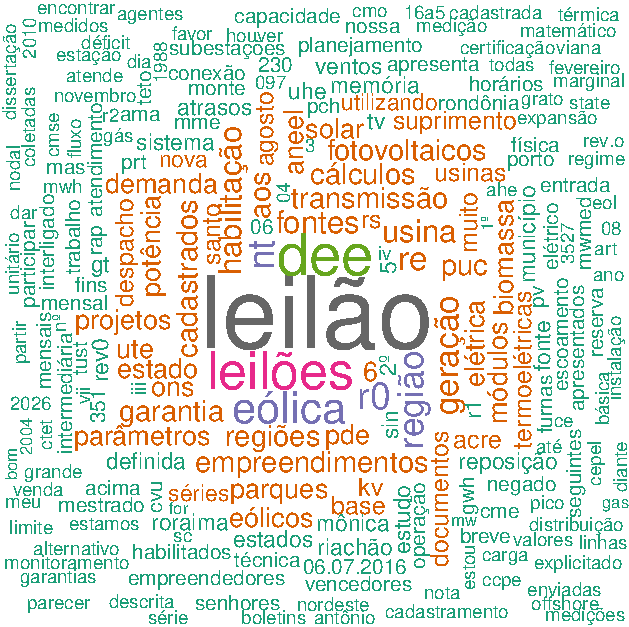
\includegraphics{markdown_v24_files/figure-latex/unnamed-chunk-44-1.pdf}

\begin{Shaded}
\begin{Highlighting}[]
\NormalTok{## DGC}
\CommentTok{#jpeg("XX_wordclou_tfidf_dir02_DGC.jpeg")}
\NormalTok{nuvem2 =}\StringTok{ }
\NormalTok{plot_diretorias_tf_dif }\OperatorTok
\StringTok{  }\KeywordTok{filter}\NormalTok{(DIRETORIA }\OperatorTok{==}\StringTok{ "DGC"}\NormalTok{) }\OperatorTok
\StringTok{  }\KeywordTok{select}\NormalTok{(}\OperatorTok{-}\NormalTok{DIRETORIA, }\DataTypeTok{word =}\NormalTok{ palavra,}\DataTypeTok{freq =}\NormalTok{ tf_idf) }\OperatorTok
\StringTok{  }\CommentTok{#top_n(150, freq) %>%}
\StringTok{  }\KeywordTok{as.data.frame}\NormalTok{() }

\KeywordTok{set.seed}\NormalTok{(}\DecValTok{75437}\NormalTok{)}
\KeywordTok{wordcloud}\NormalTok{(}\DataTypeTok{words =}\NormalTok{ nuvem2}\OperatorTok{$}\NormalTok{word, }\DataTypeTok{freq =}\NormalTok{ nuvem2}\OperatorTok{$}\NormalTok{freq, }\DataTypeTok{min.freq =} \FloatTok{0.2}\NormalTok{,}
          \DataTypeTok{max.words=}\DecValTok{250}\NormalTok{, }\DataTypeTok{random.order=}\OtherTok{FALSE}\NormalTok{, }\DataTypeTok{rot.per=}\FloatTok{0.35}\NormalTok{, }
          \DataTypeTok{colors=}\KeywordTok{brewer.pal}\NormalTok{(}\DecValTok{10}\NormalTok{, }\StringTok{"Dark2"}\NormalTok{))}
\end{Highlighting}
\end{Shaded}

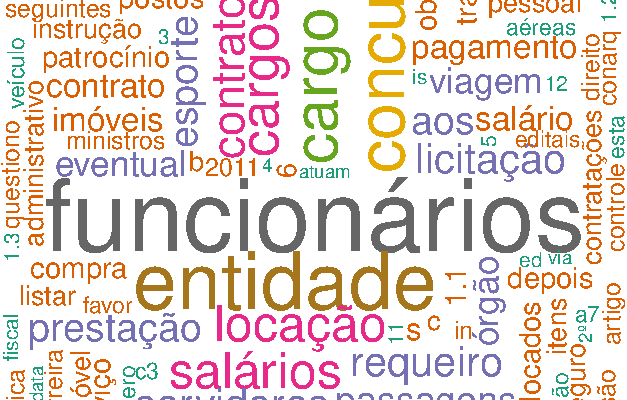
\includegraphics{markdown_v24_files/figure-latex/unnamed-chunk-44-2.pdf}

\begin{Shaded}
\begin{Highlighting}[]
\NormalTok{## DEA}
\CommentTok{#jpeg("XX_wordclou_tfidf_dir03_DEA.jpeg")}
\NormalTok{nuvem3 =}\StringTok{ }
\NormalTok{plot_diretorias_tf_dif }\OperatorTok
\StringTok{  }\KeywordTok{filter}\NormalTok{(DIRETORIA }\OperatorTok{==}\StringTok{ "DEA"}\NormalTok{) }\OperatorTok
\StringTok{  }\KeywordTok{select}\NormalTok{(}\OperatorTok{-}\NormalTok{DIRETORIA, }\DataTypeTok{word =}\NormalTok{ palavra,}\DataTypeTok{freq =}\NormalTok{ tf_idf) }\OperatorTok
\StringTok{  }\CommentTok{#top_n(150, freq) %>%}
\StringTok{  }\KeywordTok{as.data.frame}\NormalTok{() }

\KeywordTok{set.seed}\NormalTok{(}\DecValTok{231321}\NormalTok{)}
\KeywordTok{wordcloud}\NormalTok{(}\DataTypeTok{words =}\NormalTok{ nuvem3}\OperatorTok{$}\NormalTok{word, }\DataTypeTok{freq =}\NormalTok{ nuvem3}\OperatorTok{$}\NormalTok{freq, }\DataTypeTok{min.freq =} \FloatTok{0.2}\NormalTok{,}
          \DataTypeTok{max.words=}\DecValTok{250}\NormalTok{, }\DataTypeTok{random.order=}\OtherTok{FALSE}\NormalTok{, }\DataTypeTok{rot.per=}\FloatTok{0.35}\NormalTok{, }
          \DataTypeTok{colors=}\KeywordTok{brewer.pal}\NormalTok{(}\DecValTok{10}\NormalTok{, }\StringTok{"Dark2"}\NormalTok{))}
\end{Highlighting}
\end{Shaded}

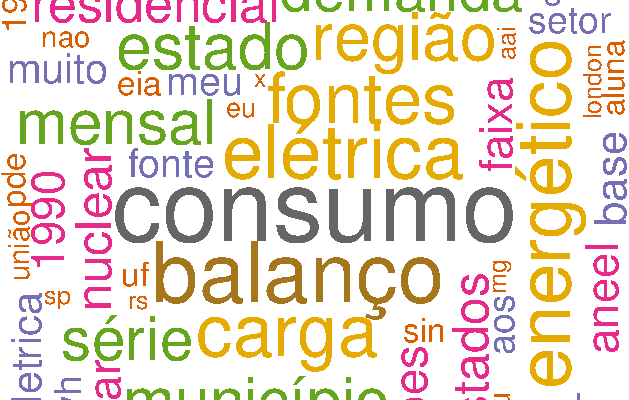
\includegraphics{markdown_v24_files/figure-latex/unnamed-chunk-44-3.pdf}

\begin{Shaded}
\begin{Highlighting}[]
\NormalTok{## DPG}
\CommentTok{#jpeg("XX_wordclou_tfidf_dir04_DPG.jpeg")}
\NormalTok{nuvem4 =}\StringTok{ }
\NormalTok{plot_diretorias_tf_dif }\OperatorTok
\StringTok{  }\KeywordTok{filter}\NormalTok{(DIRETORIA }\OperatorTok{==}\StringTok{ "DPG"}\NormalTok{) }\OperatorTok
\StringTok{  }\KeywordTok{select}\NormalTok{(}\OperatorTok{-}\NormalTok{DIRETORIA, }\DataTypeTok{word =}\NormalTok{ palavra,}\DataTypeTok{freq =}\NormalTok{ tf_idf) }\OperatorTok
\StringTok{  }\CommentTok{#top_n(150, freq) %>%}
\StringTok{  }\KeywordTok{as.data.frame}\NormalTok{() }

\KeywordTok{set.seed}\NormalTok{(}\DecValTok{75437}\NormalTok{)}
\KeywordTok{wordcloud}\NormalTok{(}\DataTypeTok{words =}\NormalTok{ nuvem4}\OperatorTok{$}\NormalTok{word, }\DataTypeTok{freq =}\NormalTok{ nuvem4}\OperatorTok{$}\NormalTok{freq, }\DataTypeTok{min.freq =} \FloatTok{0.1}\NormalTok{,}
          \DataTypeTok{max.words=}\DecValTok{250}\NormalTok{, }\DataTypeTok{random.order=}\OtherTok{FALSE}\NormalTok{, }\DataTypeTok{rot.per=}\FloatTok{0.35}\NormalTok{, }
          \DataTypeTok{colors=}\KeywordTok{brewer.pal}\NormalTok{(}\DecValTok{10}\NormalTok{, }\StringTok{"Dark2"}\NormalTok{))}
\end{Highlighting}
\end{Shaded}

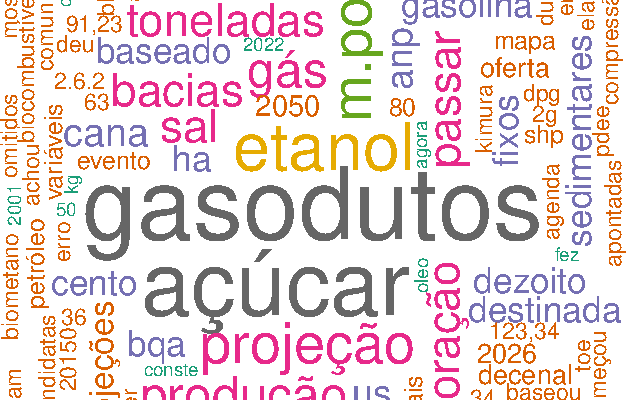
\includegraphics{markdown_v24_files/figure-latex/unnamed-chunk-44-4.pdf}

\begin{Shaded}
\begin{Highlighting}[]
\NormalTok{## OUTROS}
\CommentTok{#jpeg("XX_wordclou_tfidf_dir05_OUTROS.jpeg")}
\NormalTok{nuvem5 =}\StringTok{ }
\NormalTok{plot_diretorias_tf_dif }\OperatorTok
\StringTok{  }\KeywordTok{filter}\NormalTok{(DIRETORIA }\OperatorTok{==}\StringTok{ "OUTROS"}\NormalTok{) }\OperatorTok
\StringTok{  }\KeywordTok{select}\NormalTok{(}\OperatorTok{-}\NormalTok{DIRETORIA, }\DataTypeTok{word =}\NormalTok{ palavra,}\DataTypeTok{freq =}\NormalTok{ tf_idf) }\OperatorTok
\StringTok{  }\CommentTok{#top_n(150, freq) %>%}
\StringTok{  }\KeywordTok{as.data.frame}\NormalTok{() }

\KeywordTok{set.seed}\NormalTok{(}\DecValTok{75437}\NormalTok{)}
\KeywordTok{wordcloud}\NormalTok{(}\DataTypeTok{words =}\NormalTok{ nuvem5}\OperatorTok{$}\NormalTok{word, }\DataTypeTok{freq =}\NormalTok{ nuvem5}\OperatorTok{$}\NormalTok{freq, }\DataTypeTok{min.freq =} \FloatTok{0.1}\NormalTok{,}
          \DataTypeTok{max.words=}\DecValTok{250}\NormalTok{, }\DataTypeTok{random.order=}\OtherTok{FALSE}\NormalTok{, }\DataTypeTok{rot.per=}\FloatTok{0.35}\NormalTok{, }
          \DataTypeTok{colors=}\KeywordTok{brewer.pal}\NormalTok{(}\DecValTok{10}\NormalTok{, }\StringTok{"Dark2"}\NormalTok{))}
\end{Highlighting}
\end{Shaded}

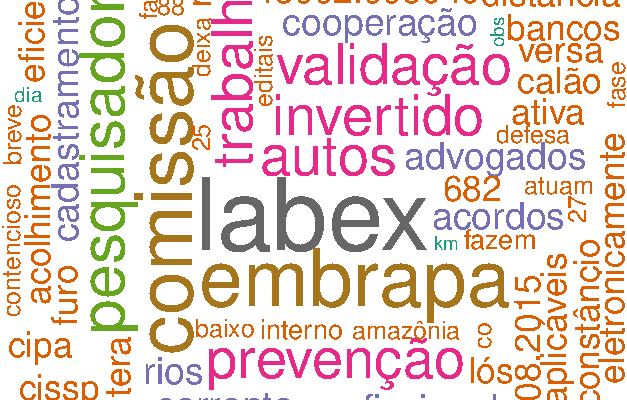
\includegraphics{markdown_v24_files/figure-latex/unnamed-chunk-44-5.pdf}

\begin{Shaded}
\begin{Highlighting}[]
\CommentTok{#View(head(plot_diretoria_palavras))}
\NormalTok{library(wordcloud2)}

\NormalTok{plot_diretorias_tf_dif = plot_diretoria_palavras %>%}
\NormalTok{    select(palavra, tf_idf, DIRETORIA) %>%}
\NormalTok{    mutate(palavra = reorder(palavra, tf_idf))}

\CommentTok{## DEE}
\CommentTok{#jpeg("XX_wordclou_tfidf_dir01_DEE.jpeg")}
\NormalTok{set.seed(233115)}
\NormalTok{plot_diretorias_tf_dif %>%}
\NormalTok{  filter(DIRETORIA == }\StringTok{"DEE"}\NormalTok{) %>%}
\NormalTok{  top_n(150, tf_idf) %>%}
\NormalTok{  wordcloud2(shuffle = TRUE, }
\NormalTok{             color = }\StringTok{"random-dark"}\NormalTok{,}
\NormalTok{             shape = }\StringTok{"circle"}\NormalTok{)}

\CommentTok{## DGC}
\CommentTok{#jpeg("XX_wordclou_tfidf_dir01_DGC.jpeg")}
\NormalTok{set.seed(233115)}
\NormalTok{plot_diretorias_tf_dif %>%}
\NormalTok{  filter(DIRETORIA == }\StringTok{"DGC"}\NormalTok{) %>%}
\NormalTok{  top_n(150, tf_idf) %>%}
\NormalTok{  wordcloud2()}

\CommentTok{## DEA}
\CommentTok{#jpeg("XX_wordclou_tfidf_dir01_DEA.jpeg")}
\NormalTok{set.seed(233115)}
\NormalTok{plot_diretorias_tf_dif %>%}
\NormalTok{  filter(DIRETORIA == }\StringTok{"DEA"}\NormalTok{) %>%}
\NormalTok{  top_n(150, tf_idf) %>%}
\NormalTok{  wordcloud2()}

\CommentTok{## DPG}
\CommentTok{#jpeg("XX_wordclou_tfidf_dir04_DPG.jpeg")}
\NormalTok{set.seed(233115)}
\NormalTok{plot_diretorias_tf_dif %>%}
\NormalTok{  filter(DIRETORIA == }\StringTok{"DPG"}\NormalTok{) %>%}
\NormalTok{  top_n(150, tf_idf) %>%}
\NormalTok{  wordcloud2()}
  
\CommentTok{## OUTROS}
\CommentTok{#jpeg("XX_wordclou_tfidf_dir01_OUTROS.jpeg")}
\NormalTok{set.seed(233115)}
\NormalTok{plot_diretorias_tf_dif %>%}
\NormalTok{  filter(DIRETORIA == }\StringTok{"OUTROS"}\NormalTok{) %>%}
\NormalTok{  top_n(150, tf_idf) %>%}
\NormalTok{  wordcloud2()}
\end{Highlighting}
\end{Shaded}

--\textgreater{}

\paragraph{Nuvem de palavras por diretoria - s/ steeming e/ou remoção de
stopwords -
bigram}\label{nuvem-de-palavras-por-diretoria---s-steeming-eou-remocao-de-stopwords---bigram}

\begin{Shaded}
\begin{Highlighting}[]
\NormalTok{plot_diretorias_tf_dif_bigram =}\StringTok{ }\NormalTok{DB }\OperatorTok
\StringTok{  }\KeywordTok{select}\NormalTok{(DESCRI_PEDIDO,DIRETORIA) }\OperatorTok
\StringTok{  }\KeywordTok{unnest_tokens}\NormalTok{(BIGRAM, DESCRI_PEDIDO, }\DataTypeTok{token =} \StringTok{"ngrams"}\NormalTok{, }\DataTypeTok{n =} \DecValTok{2}\NormalTok{) }\OperatorTok
\StringTok{  }\KeywordTok{count}\NormalTok{(DIRETORIA, BIGRAM, }\DataTypeTok{sort =} \OtherTok{TRUE}\NormalTok{) }\OperatorTok
\StringTok{  }\KeywordTok{bind_tf_idf}\NormalTok{(BIGRAM, DIRETORIA, n) }\OperatorTok
\StringTok{  }\KeywordTok{arrange}\NormalTok{(}\KeywordTok{desc}\NormalTok{(tf_idf)) }\OperatorTok
\StringTok{  }\KeywordTok{mutate}\NormalTok{(}\DataTypeTok{BIGRAM =} \KeywordTok{factor}\NormalTok{(BIGRAM, }\DataTypeTok{levels =} \KeywordTok{rev}\NormalTok{(}\KeywordTok{unique}\NormalTok{(BIGRAM)))) }\OperatorTok
\StringTok{  }\KeywordTok{mutate}\NormalTok{(}\DataTypeTok{DIRETORIA =} \KeywordTok{factor}\NormalTok{(DIRETORIA,}\DataTypeTok{levels=}\KeywordTok{c}\NormalTok{(}\StringTok{"DEA"}\NormalTok{,}\StringTok{"DEE"}\NormalTok{,}\StringTok{"DGC"}\NormalTok{,}\StringTok{"DPG"}\NormalTok{,}\StringTok{"OUTROS"}\NormalTok{))) }\OperatorTok
\StringTok{  }\KeywordTok{select}\NormalTok{(BIGRAM, tf_idf, DIRETORIA)}
\end{Highlighting}
\end{Shaded}

\begin{Shaded}
\begin{Highlighting}[]
\NormalTok{## DEE}
\CommentTok{#jpeg("XX_wordclou_tfidf_dir01_DEE.jpeg")}
\NormalTok{nuvem1.}\DecValTok{2}\NormalTok{ =}\StringTok{ }
\NormalTok{plot_diretorias_tf_dif_bigram }\OperatorTok
\StringTok{  }\KeywordTok{filter}\NormalTok{(DIRETORIA }\OperatorTok{==}\StringTok{ "DEE"}\NormalTok{) }\OperatorTok
\StringTok{  }\KeywordTok{select}\NormalTok{(}\OperatorTok{-}\NormalTok{DIRETORIA, }\DataTypeTok{word =}\NormalTok{ BIGRAM,}\DataTypeTok{freq =}\NormalTok{ tf_idf) }\OperatorTok
\StringTok{  }\CommentTok{#top_n(150, freq) %>%}
\StringTok{  }\KeywordTok{as.data.frame}\NormalTok{() }

\KeywordTok{set.seed}\NormalTok{(}\DecValTok{231321}\NormalTok{)}
\KeywordTok{wordcloud}\NormalTok{(}\DataTypeTok{words =}\NormalTok{ nuvem1.}\DecValTok{2}\OperatorTok{$}\NormalTok{word, }\DataTypeTok{freq =}\NormalTok{ nuvem1.}\DecValTok{2}\OperatorTok{$}\NormalTok{freq, }\DataTypeTok{min.freq =} \FloatTok{0.2}\NormalTok{,}
          \DataTypeTok{max.words=}\DecValTok{250}\NormalTok{, }\DataTypeTok{random.order=}\OtherTok{FALSE}\NormalTok{, }\DataTypeTok{rot.per=}\FloatTok{0.35}\NormalTok{, }
          \DataTypeTok{colors=}\KeywordTok{brewer.pal}\NormalTok{(}\DecValTok{10}\NormalTok{, }\StringTok{"Dark2"}\NormalTok{))}
\end{Highlighting}
\end{Shaded}

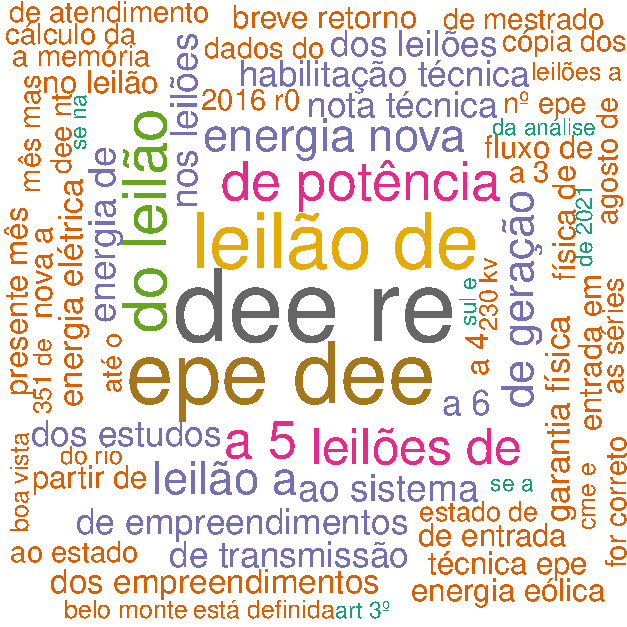
\includegraphics{markdown_v24_files/figure-latex/wordcloud_onegram_DIR01_semstopwords-1.pdf}

\begin{Shaded}
\begin{Highlighting}[]
\NormalTok{## DGC}
\CommentTok{#jpeg("XX_wordclou_tfidf_dir02_DGC.jpeg")}
\NormalTok{nuvem2.}\DecValTok{2}\NormalTok{ =}\StringTok{ }
\NormalTok{plot_diretorias_tf_dif_bigram }\OperatorTok
\StringTok{  }\KeywordTok{filter}\NormalTok{(DIRETORIA }\OperatorTok{==}\StringTok{ "DGC"}\NormalTok{) }\OperatorTok
\StringTok{  }\KeywordTok{select}\NormalTok{(}\OperatorTok{-}\NormalTok{DIRETORIA, }\DataTypeTok{word =}\NormalTok{ BIGRAM,}\DataTypeTok{freq =}\NormalTok{ tf_idf) }\OperatorTok
\StringTok{  }\CommentTok{#top_n(150, freq) %>%}
\StringTok{  }\KeywordTok{as.data.frame}\NormalTok{() }

\KeywordTok{set.seed}\NormalTok{(}\DecValTok{75437}\NormalTok{)}
\KeywordTok{wordcloud}\NormalTok{(}\DataTypeTok{words =}\NormalTok{ nuvem2.}\DecValTok{2}\OperatorTok{$}\NormalTok{word, }\DataTypeTok{freq =}\NormalTok{ nuvem2.}\DecValTok{2}\OperatorTok{$}\NormalTok{freq, }\DataTypeTok{min.freq =} \FloatTok{0.2}\NormalTok{,}
          \DataTypeTok{max.words=}\DecValTok{250}\NormalTok{, }\DataTypeTok{random.order=}\OtherTok{FALSE}\NormalTok{, }\DataTypeTok{rot.per=}\FloatTok{0.35}\NormalTok{, }
          \DataTypeTok{colors=}\KeywordTok{brewer.pal}\NormalTok{(}\DecValTok{10}\NormalTok{, }\StringTok{"Dark2"}\NormalTok{))}
\end{Highlighting}
\end{Shaded}

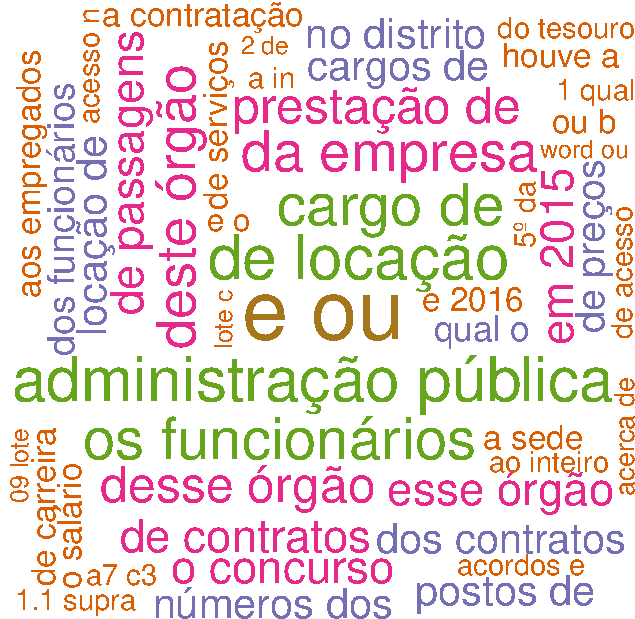
\includegraphics{markdown_v24_files/figure-latex/wordcloud_onegram_DIR02_semstopwords-1.pdf}

\begin{Shaded}
\begin{Highlighting}[]
\NormalTok{## DEA}
\CommentTok{#jpeg("XX_wordclou_tfidf_dir03_DEA.jpeg")}
\NormalTok{nuvem3.}\DecValTok{2}\NormalTok{ =}\StringTok{ }
\NormalTok{plot_diretorias_tf_dif_bigram }\OperatorTok
\StringTok{  }\KeywordTok{filter}\NormalTok{(DIRETORIA }\OperatorTok{==}\StringTok{ "DEA"}\NormalTok{) }\OperatorTok
\StringTok{  }\KeywordTok{select}\NormalTok{(}\OperatorTok{-}\NormalTok{DIRETORIA, }\DataTypeTok{word =}\NormalTok{ BIGRAM,}\DataTypeTok{freq =}\NormalTok{ tf_idf) }\OperatorTok
\StringTok{  }\CommentTok{#top_n(150, freq) %>%}
\StringTok{  }\KeywordTok{as.data.frame}\NormalTok{() }

\KeywordTok{set.seed}\NormalTok{(}\DecValTok{543453}\NormalTok{)}
\KeywordTok{wordcloud}\NormalTok{(}\DataTypeTok{words =}\NormalTok{ nuvem3.}\DecValTok{2}\OperatorTok{$}\NormalTok{word, }\DataTypeTok{freq =}\NormalTok{ nuvem3.}\DecValTok{2}\OperatorTok{$}\NormalTok{freq, }\DataTypeTok{min.freq =} \FloatTok{0.2}\NormalTok{,}
          \DataTypeTok{max.words=}\DecValTok{250}\NormalTok{, }\DataTypeTok{random.order=}\OtherTok{FALSE}\NormalTok{, }\DataTypeTok{rot.per=}\FloatTok{0.35}\NormalTok{, }
          \DataTypeTok{colors=}\KeywordTok{brewer.pal}\NormalTok{(}\DecValTok{10}\NormalTok{, }\StringTok{"Dark2"}\NormalTok{))}
\end{Highlighting}
\end{Shaded}

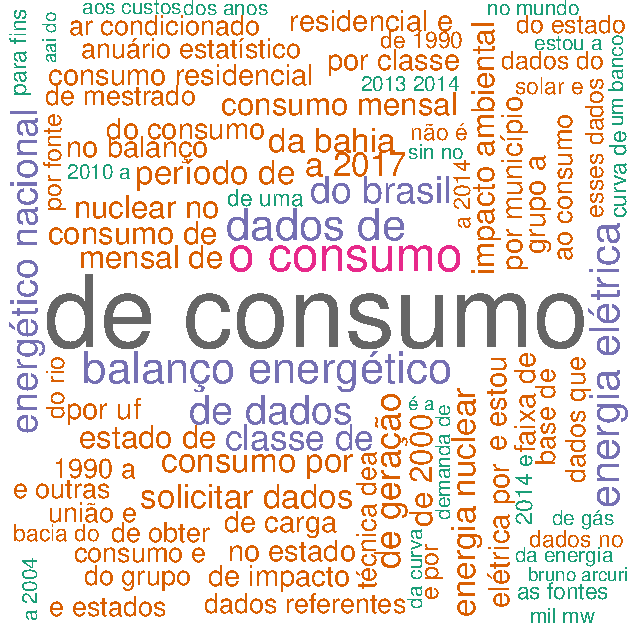
\includegraphics{markdown_v24_files/figure-latex/wordcloud_onegram_DIR03_semstopwords-1.pdf}

\begin{Shaded}
\begin{Highlighting}[]
\NormalTok{## DPG}
\CommentTok{#jpeg("XX_wordclou_tfidf_dir04_DPG.jpeg")}
\NormalTok{nuvem4.}\DecValTok{2}\NormalTok{ =}\StringTok{ }
\NormalTok{plot_diretorias_tf_dif_bigram }\OperatorTok
\StringTok{  }\KeywordTok{filter}\NormalTok{(DIRETORIA }\OperatorTok{==}\StringTok{ "DPG"}\NormalTok{) }\OperatorTok
\StringTok{  }\KeywordTok{select}\NormalTok{(}\OperatorTok{-}\NormalTok{DIRETORIA, }\DataTypeTok{word =}\NormalTok{ BIGRAM,}\DataTypeTok{freq =}\NormalTok{ tf_idf) }\OperatorTok
\StringTok{  }\CommentTok{#top_n(150, freq) %>%}
\StringTok{  }\KeywordTok{as.data.frame}\NormalTok{() }

\KeywordTok{set.seed}\NormalTok{(}\DecValTok{75437}\NormalTok{)}
\KeywordTok{wordcloud}\NormalTok{(}\DataTypeTok{words =}\NormalTok{ nuvem4.}\DecValTok{2}\OperatorTok{$}\NormalTok{word, }\DataTypeTok{freq =}\NormalTok{ nuvem4.}\DecValTok{2}\OperatorTok{$}\NormalTok{freq, }\DataTypeTok{min.freq =} \FloatTok{0.1}\NormalTok{,}
          \DataTypeTok{max.words=}\DecValTok{250}\NormalTok{, }\DataTypeTok{random.order=}\OtherTok{FALSE}\NormalTok{, }\DataTypeTok{rot.per=}\FloatTok{0.35}\NormalTok{, }
          \DataTypeTok{colors=}\KeywordTok{brewer.pal}\NormalTok{(}\DecValTok{10}\NormalTok{, }\StringTok{"Dark2"}\NormalTok{))}
\end{Highlighting}
\end{Shaded}

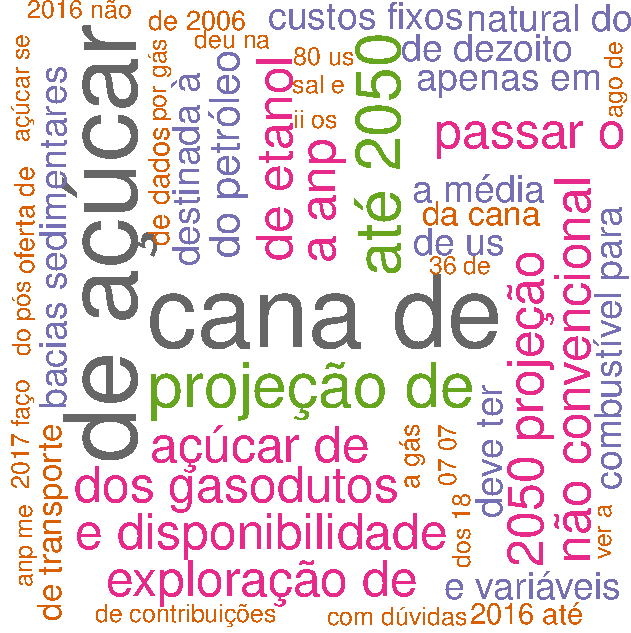
\includegraphics{markdown_v24_files/figure-latex/wordcloud_onegram_DIR04_semstopwords-1.pdf}

\begin{Shaded}
\begin{Highlighting}[]
\NormalTok{## OUTROS}
\CommentTok{#jpeg("XX_wordclou_tfidf_dir05_OUTROS.jpeg")}
\NormalTok{nuvem5.}\DecValTok{2}\NormalTok{ =}\StringTok{ }
\NormalTok{plot_diretorias_tf_dif_bigram }\OperatorTok
\StringTok{  }\KeywordTok{filter}\NormalTok{(DIRETORIA }\OperatorTok{==}\StringTok{ "OUTROS"}\NormalTok{) }\OperatorTok
\StringTok{  }\KeywordTok{select}\NormalTok{(}\OperatorTok{-}\NormalTok{DIRETORIA, }\DataTypeTok{word =}\NormalTok{ BIGRAM,}\DataTypeTok{freq =}\NormalTok{ tf_idf) }\OperatorTok
\StringTok{  }\CommentTok{#top_n(150, freq) %>%}
\StringTok{  }\KeywordTok{as.data.frame}\NormalTok{() }

\KeywordTok{set.seed}\NormalTok{(}\DecValTok{75437}\NormalTok{)}
\KeywordTok{wordcloud}\NormalTok{(}\DataTypeTok{words =}\NormalTok{ nuvem5.}\DecValTok{2}\OperatorTok{$}\NormalTok{word, }\DataTypeTok{freq =}\NormalTok{ nuvem5.}\DecValTok{2}\OperatorTok{$}\NormalTok{freq, }\DataTypeTok{min.freq =} \FloatTok{0.1}\NormalTok{,}
          \DataTypeTok{max.words=}\DecValTok{250}\NormalTok{, }\DataTypeTok{random.order=}\OtherTok{FALSE}\NormalTok{, }\DataTypeTok{rot.per=}\FloatTok{0.35}\NormalTok{, }
          \DataTypeTok{colors=}\KeywordTok{brewer.pal}\NormalTok{(}\DecValTok{10}\NormalTok{, }\StringTok{"Dark2"}\NormalTok{))}
\end{Highlighting}
\end{Shaded}

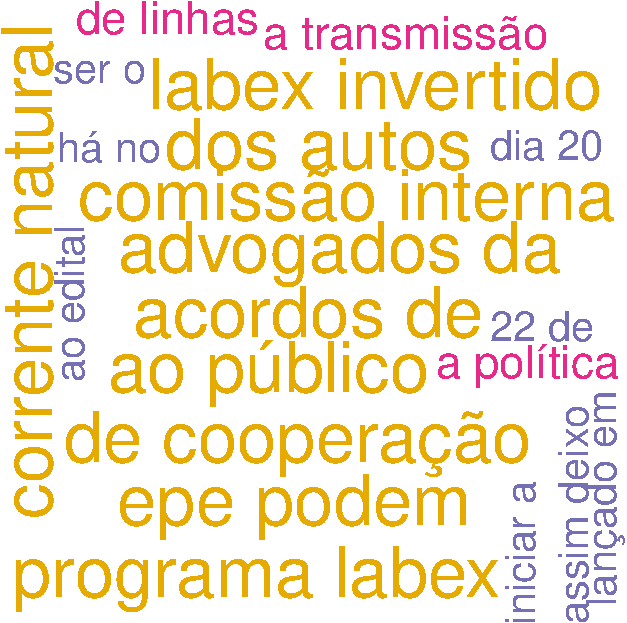
\includegraphics{markdown_v24_files/figure-latex/wordcloud_onegram_DIR05_semstopwords-1.pdf}

\begin{Shaded}
\begin{Highlighting}[]
\CommentTok{#View(head(plot_diretoria_palavras))}
\NormalTok{library(wordcloud2)}

\NormalTok{plot_diretorias_tf_dif_bigram = DB %>%}
\NormalTok{  select(DESCRI_PEDIDO,DIRETORIA) %>%}
\NormalTok{  unnest_tokens(BIGRAM, DESCRI_PEDIDO, token = }\StringTok{"ngrams"}\NormalTok{, n = 2) %>%}
\NormalTok{  count(DIRETORIA, BIGRAM, sort = TRUE) %>%}
\NormalTok{  bind_tf_idf(BIGRAM, DIRETORIA, n) %>%}
\NormalTok{  arrange(desc(tf_idf)) %>%}
\NormalTok{  mutate(BIGRAM = factor(BIGRAM, levels = rev(unique(BIGRAM)))) %>%}
\NormalTok{  mutate(DIRETORIA = factor(DIRETORIA,levels=c(}\StringTok{"DEA"}\NormalTok{,}\StringTok{"DEE"}\NormalTok{,}\StringTok{"DGC"}\NormalTok{,}\StringTok{"DPG"}\NormalTok{,}\StringTok{"OUTROS"}\NormalTok{))) %>%}
\NormalTok{  select(BIGRAM, tf_idf, DIRETORIA)}
  

\CommentTok{## DEE}
\CommentTok{#jpeg("XX_wordclou_tfidf_dir01_DEE.jpeg")}
\NormalTok{set.seed(233115)}
\NormalTok{plot_diretorias_tf_dif_bigram %>%}
\NormalTok{  filter(DIRETORIA == }\StringTok{"DEE"}\NormalTok{) %>%}
\NormalTok{  top_n(150, tf_idf) %>%}
\NormalTok{  wordcloud2(shuffle = TRUE, }
\NormalTok{             color = }\StringTok{"random-dark"}\NormalTok{,}
\NormalTok{             shape = }\StringTok{"circle"}\NormalTok{)}

\CommentTok{## DGC}
\CommentTok{#jpeg("XX_wordclou_tfidf_dir01_DGC.jpeg")}
\NormalTok{set.seed(233115)}
\NormalTok{plot_diretorias_tf_dif_bigram %>%}
\NormalTok{  filter(DIRETORIA == }\StringTok{"DGC"}\NormalTok{) %>%}
\NormalTok{  top_n(150, tf_idf) %>%}
\NormalTok{  wordcloud2()}

\CommentTok{## DEA}
\CommentTok{#jpeg("XX_wordclou_tfidf_dir01_DEA.jpeg")}
\NormalTok{set.seed(233115)}
\NormalTok{plot_diretorias_tf_dif_bigram %>%}
\NormalTok{  filter(DIRETORIA == }\StringTok{"DEA"}\NormalTok{) %>%}
\NormalTok{  top_n(150, tf_idf) %>%}
\NormalTok{  wordcloud2()}

\CommentTok{## DPG}
\CommentTok{#jpeg("XX_wordclou_tfidf_dir01_DPG.jpeg")}
\NormalTok{set.seed(233115)}
\NormalTok{plot_diretorias_tf_dif_bigram %>%}
\NormalTok{  filter(DIRETORIA == }\StringTok{"DPG"}\NormalTok{) %>%}
\NormalTok{  top_n(150, tf_idf) %>%}
\NormalTok{  wordcloud2()}
\end{Highlighting}
\end{Shaded}

\subparagraph{\texorpdfstring{Separando palavras de um bigram em
``palavra1'' e ``palavra2'' p/ remover
stopwords}{Separando palavras de um bigram em palavra1 e palavra2 p/ remover stopwords}}\label{separando-palavras-de-um-bigram-em-palavra1-e-palavra2-p-remover-stopwords}

Considerando já a exclusão de casos onde houver stopwords consecultivos
na ``palavra1'' e ``palavra2'', ou seja onde
\(palavra1=stopword \land palavra2=stopword\)

\begin{Shaded}
\begin{Highlighting}[]
\NormalTok{bigrams =}\StringTok{ }\NormalTok{DB }\OperatorTok
\StringTok{  }\KeywordTok{select}\NormalTok{(DESCRI_PEDIDO,DIRETORIA) }\OperatorTok
\StringTok{  }\KeywordTok{unnest_tokens}\NormalTok{(BIGRAM, DESCRI_PEDIDO, }\DataTypeTok{token =} \StringTok{"ngrams"}\NormalTok{, }\DataTypeTok{n =} \DecValTok{2}\NormalTok{) }\OperatorTok
\StringTok{  }\KeywordTok{count}\NormalTok{(DIRETORIA, BIGRAM, }\DataTypeTok{sort =} \OtherTok{TRUE}\NormalTok{) }

\NormalTok{separa_bigrams =}\StringTok{ }\NormalTok{bigrams }\OperatorTok
\StringTok{  }\KeywordTok{separate}\NormalTok{(BIGRAM, }\KeywordTok{c}\NormalTok{(}\StringTok{"palavra1"}\NormalTok{, }\StringTok{"palavra2"}\NormalTok{), }\DataTypeTok{sep =} \StringTok{" "}\NormalTok{)}

\NormalTok{junta_bigrams =}\StringTok{ }\NormalTok{separa_bigrams }\OperatorTok
\StringTok{  }\KeywordTok{unite}\NormalTok{(BIGRAM, palavra1, palavra2, }\DataTypeTok{sep =} \StringTok{" "}\NormalTok{)}
\CommentTok{# levels(as.factor(junta_bigrams$BIGRAM == bigrams$BIGRAM))   # CHECK}

\NormalTok{## remove stopwords  }
\NormalTok{bigrams2 =}\StringTok{ }\KeywordTok{cbind}\NormalTok{(separa_bigrams,}\DataTypeTok{BIGRAM =}\NormalTok{ junta_bigrams}\OperatorTok{$}\NormalTok{BIGRAM) }\OperatorTok
\StringTok{  }\KeywordTok{filter}\NormalTok{(}\OperatorTok{!}\NormalTok{palavra1 }\OperatorTok\StringTok{ }\NormalTok{mystopwords}\OperatorTok{$}\NormalTok{palavra) }\OperatorTok
\StringTok{  }\KeywordTok{filter}\NormalTok{(}\OperatorTok{!}\NormalTok{palavra2 }\OperatorTok\StringTok{ }\NormalTok{mystopwords}\OperatorTok{$}\NormalTok{palavra) }\OperatorTok\StringTok{  }
\StringTok{  }\KeywordTok{filter}\NormalTok{(}\OperatorTok{!}\NormalTok{palavra1 }\OperatorTok\StringTok{ "a"}\NormalTok{) }\OperatorTok
\StringTok{  }\KeywordTok{filter}\NormalTok{(}\OperatorTok{!}\NormalTok{palavra2 }\OperatorTok\StringTok{ "a"}\NormalTok{) }\OperatorTok
\StringTok{  }\KeywordTok{filter}\NormalTok{(}\OperatorTok{!}\NormalTok{palavra1 }\OperatorTok\StringTok{ "p"}\NormalTok{) }\OperatorTok
\StringTok{  }\KeywordTok{filter}\NormalTok{(}\OperatorTok{!}\NormalTok{palavra1 }\OperatorTok\StringTok{ "s"}\NormalTok{) }\OperatorTok
\StringTok{  }\KeywordTok{filter}\NormalTok{(}\OperatorTok{!}\NormalTok{palavra1 }\OperatorTok\StringTok{ "d"}\NormalTok{) }\OperatorTok
\StringTok{  }\KeywordTok{filter}\NormalTok{(}\OperatorTok{!}\NormalTok{palavra2 }\OperatorTok\StringTok{ "p"}\NormalTok{) }\OperatorTok
\StringTok{  }\KeywordTok{filter}\NormalTok{(}\OperatorTok{!}\NormalTok{palavra2 }\OperatorTok\StringTok{ "s"}\NormalTok{) }\OperatorTok
\StringTok{  }\KeywordTok{filter}\NormalTok{(}\OperatorTok{!}\NormalTok{palavra2 }\OperatorTok\StringTok{ "d"}\NormalTok{) }\OperatorTok
\StringTok{  }\KeywordTok{filter}\NormalTok{(}\OperatorTok{!}\NormalTok{palavra2 }\OperatorTok\StringTok{ "s.a"}\NormalTok{) }\OperatorTok
\StringTok{  }\KeywordTok{filter}\NormalTok{(}\OperatorTok{!}\KeywordTok{str_detect}\NormalTok{(palavra1, }\StringTok{"0"}\NormalTok{)) }\OperatorTok
\StringTok{  }\KeywordTok{filter}\NormalTok{(}\OperatorTok{!}\KeywordTok{str_detect}\NormalTok{(palavra1, }\StringTok{"1"}\NormalTok{)) }\OperatorTok
\StringTok{  }\KeywordTok{filter}\NormalTok{(}\OperatorTok{!}\KeywordTok{str_detect}\NormalTok{(palavra1, }\StringTok{"2"}\NormalTok{)) }\OperatorTok
\StringTok{  }\KeywordTok{filter}\NormalTok{(}\OperatorTok{!}\KeywordTok{str_detect}\NormalTok{(palavra1, }\StringTok{"3"}\NormalTok{)) }\OperatorTok
\StringTok{  }\KeywordTok{filter}\NormalTok{(}\OperatorTok{!}\KeywordTok{str_detect}\NormalTok{(palavra1, }\StringTok{"4"}\NormalTok{)) }\OperatorTok
\StringTok{  }\KeywordTok{filter}\NormalTok{(}\OperatorTok{!}\KeywordTok{str_detect}\NormalTok{(palavra1, }\StringTok{"5"}\NormalTok{)) }\OperatorTok
\StringTok{  }\KeywordTok{filter}\NormalTok{(}\OperatorTok{!}\KeywordTok{str_detect}\NormalTok{(palavra1, }\StringTok{"6"}\NormalTok{)) }\OperatorTok
\StringTok{  }\KeywordTok{filter}\NormalTok{(}\OperatorTok{!}\KeywordTok{str_detect}\NormalTok{(palavra1, }\StringTok{"7"}\NormalTok{)) }\OperatorTok
\StringTok{  }\KeywordTok{filter}\NormalTok{(}\OperatorTok{!}\KeywordTok{str_detect}\NormalTok{(palavra1, }\StringTok{"8"}\NormalTok{)) }\OperatorTok
\StringTok{  }\KeywordTok{filter}\NormalTok{(}\OperatorTok{!}\KeywordTok{str_detect}\NormalTok{(palavra1, }\StringTok{"9"}\NormalTok{)) }\OperatorTok
\StringTok{  }\KeywordTok{filter}\NormalTok{(}\OperatorTok{!}\KeywordTok{str_detect}\NormalTok{(palavra2, }\StringTok{"0"}\NormalTok{)) }\OperatorTok
\StringTok{  }\KeywordTok{filter}\NormalTok{(}\OperatorTok{!}\KeywordTok{str_detect}\NormalTok{(palavra2, }\StringTok{"1"}\NormalTok{)) }\OperatorTok
\StringTok{  }\KeywordTok{filter}\NormalTok{(}\OperatorTok{!}\KeywordTok{str_detect}\NormalTok{(palavra2, }\StringTok{"2"}\NormalTok{)) }\OperatorTok
\StringTok{  }\KeywordTok{filter}\NormalTok{(}\OperatorTok{!}\KeywordTok{str_detect}\NormalTok{(palavra2, }\StringTok{"3"}\NormalTok{)) }\OperatorTok
\StringTok{  }\KeywordTok{filter}\NormalTok{(}\OperatorTok{!}\KeywordTok{str_detect}\NormalTok{(palavra2, }\StringTok{"4"}\NormalTok{)) }\OperatorTok
\StringTok{  }\KeywordTok{filter}\NormalTok{(}\OperatorTok{!}\KeywordTok{str_detect}\NormalTok{(palavra2, }\StringTok{"5"}\NormalTok{)) }\OperatorTok
\StringTok{  }\KeywordTok{filter}\NormalTok{(}\OperatorTok{!}\KeywordTok{str_detect}\NormalTok{(palavra2, }\StringTok{"6"}\NormalTok{)) }\OperatorTok
\StringTok{  }\KeywordTok{filter}\NormalTok{(}\OperatorTok{!}\KeywordTok{str_detect}\NormalTok{(palavra2, }\StringTok{"7"}\NormalTok{)) }\OperatorTok
\StringTok{  }\KeywordTok{filter}\NormalTok{(}\OperatorTok{!}\KeywordTok{str_detect}\NormalTok{(palavra2, }\StringTok{"8"}\NormalTok{)) }\OperatorTok
\StringTok{  }\KeywordTok{filter}\NormalTok{(}\OperatorTok{!}\KeywordTok{str_detect}\NormalTok{(palavra2, }\StringTok{"9"}\NormalTok{))}
  \CommentTok{#count(DIRETORIA, BIGRAM) }
\end{Highlighting}
\end{Shaded}

\paragraph{Nuvem de palavras por diretoria - s/ steeming c/ remoção de
stopwords -
bigram}\label{nuvem-de-palavras-por-diretoria---s-steeming-c-remocao-de-stopwords---bigram}

\begin{Shaded}
\begin{Highlighting}[]
\CommentTok{#View(head(plot_diretoria_palavras))}
\KeywordTok{library}\NormalTok{(wordcloud2)}
\KeywordTok{library}\NormalTok{(wordcloud)}
\NormalTok{plot_diretorias_tf_dif_bigram2 =}\StringTok{ }\NormalTok{bigrams2 }\OperatorTok
\StringTok{  }\KeywordTok{select}\NormalTok{(BIGRAM,n,DIRETORIA) }\OperatorTok
\StringTok{  }\KeywordTok{bind_tf_idf}\NormalTok{(BIGRAM, DIRETORIA, n) }\OperatorTok
\StringTok{  }\KeywordTok{arrange}\NormalTok{(}\KeywordTok{desc}\NormalTok{(tf_idf)) }\OperatorTok
\StringTok{  }\KeywordTok{mutate}\NormalTok{(}\DataTypeTok{BIGRAM =} \KeywordTok{factor}\NormalTok{(BIGRAM, }\DataTypeTok{levels =} \KeywordTok{rev}\NormalTok{(}\KeywordTok{unique}\NormalTok{(BIGRAM)))) }\OperatorTok
\StringTok{  }\KeywordTok{mutate}\NormalTok{(}\DataTypeTok{DIRETORIA =} \KeywordTok{factor}\NormalTok{(DIRETORIA,}\DataTypeTok{levels=}\KeywordTok{c}\NormalTok{(}\StringTok{"DEA"}\NormalTok{,}\StringTok{"DEE"}\NormalTok{,}\StringTok{"DGC"}\NormalTok{,}\StringTok{"DPG"}\NormalTok{,}\StringTok{"OUTROS"}\NormalTok{))) }\OperatorTok
\StringTok{  }\KeywordTok{select}\NormalTok{(BIGRAM, tf_idf, DIRETORIA)}
\end{Highlighting}
\end{Shaded}

\begin{Shaded}
\begin{Highlighting}[]
\NormalTok{## DEE}
\CommentTok{#jpeg("XX_wordclou_tfidf_dir01_DEE.jpeg")}
\NormalTok{nuvem1.}\DecValTok{2}\NormalTok{ =}\StringTok{ }
\NormalTok{plot_diretorias_tf_dif_bigram2 }\OperatorTok
\StringTok{  }\KeywordTok{filter}\NormalTok{(DIRETORIA }\OperatorTok{==}\StringTok{ "DEE"}\NormalTok{) }\OperatorTok
\StringTok{  }\KeywordTok{select}\NormalTok{(}\OperatorTok{-}\NormalTok{DIRETORIA, }\DataTypeTok{word =}\NormalTok{ BIGRAM,}\DataTypeTok{freq =}\NormalTok{ tf_idf) }\OperatorTok
\StringTok{  }\CommentTok{#top_n(150, freq) %>%}
\StringTok{  }\KeywordTok{as.data.frame}\NormalTok{() }

\KeywordTok{set.seed}\NormalTok{(}\DecValTok{231321}\NormalTok{)}
\KeywordTok{wordcloud}\NormalTok{(}\DataTypeTok{words =}\NormalTok{ nuvem1.}\DecValTok{2}\OperatorTok{$}\NormalTok{word, }\DataTypeTok{freq =}\NormalTok{ nuvem1.}\DecValTok{2}\OperatorTok{$}\NormalTok{freq, }\DataTypeTok{min.freq =} \FloatTok{0.2}\NormalTok{,}
          \DataTypeTok{max.words=}\DecValTok{250}\NormalTok{, }\DataTypeTok{random.order=}\OtherTok{FALSE}\NormalTok{, }\DataTypeTok{rot.per=}\FloatTok{0.35}\NormalTok{, }
          \DataTypeTok{colors=}\KeywordTok{brewer.pal}\NormalTok{(}\DecValTok{10}\NormalTok{, }\StringTok{"Dark2"}\NormalTok{))}
\end{Highlighting}
\end{Shaded}

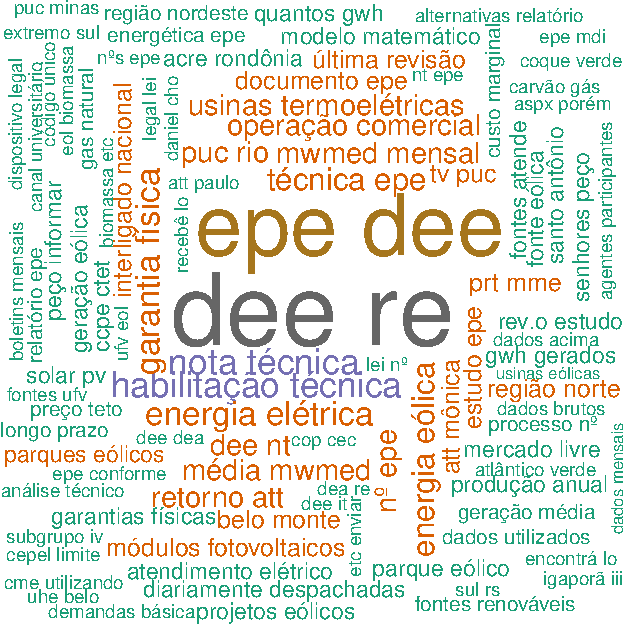
\includegraphics{markdown_v24_files/figure-latex/wordcloud_bigram_DIR01_semstopwords-1.pdf}

\begin{Shaded}
\begin{Highlighting}[]
\NormalTok{## DGC}
\CommentTok{#jpeg("XX_wordclou_tfidf_dir02_DGC.jpeg")}
\NormalTok{nuvem2.}\DecValTok{2}\NormalTok{ =}\StringTok{ }
\NormalTok{plot_diretorias_tf_dif_bigram2 }\OperatorTok
\StringTok{  }\KeywordTok{filter}\NormalTok{(DIRETORIA }\OperatorTok{==}\StringTok{ "DGC"}\NormalTok{) }\OperatorTok
\StringTok{  }\KeywordTok{select}\NormalTok{(}\OperatorTok{-}\NormalTok{DIRETORIA, }\DataTypeTok{word =}\NormalTok{ BIGRAM,}\DataTypeTok{freq =}\NormalTok{ tf_idf) }\OperatorTok
\StringTok{  }\CommentTok{#top_n(150, freq) %>%}
\StringTok{  }\KeywordTok{as.data.frame}\NormalTok{() }

\KeywordTok{set.seed}\NormalTok{(}\DecValTok{95654}\NormalTok{)}
\KeywordTok{wordcloud}\NormalTok{(}\DataTypeTok{words =}\NormalTok{ nuvem2.}\DecValTok{2}\OperatorTok{$}\NormalTok{word, }\DataTypeTok{freq =}\NormalTok{ nuvem2.}\DecValTok{2}\OperatorTok{$}\NormalTok{freq,}
          \DataTypeTok{max.words=}\DecValTok{250}\NormalTok{, }\DataTypeTok{random.order=}\OtherTok{FALSE}\NormalTok{, }\DataTypeTok{rot.per=}\FloatTok{0.35}\NormalTok{, }
          \DataTypeTok{colors=}\KeywordTok{brewer.pal}\NormalTok{(}\DecValTok{10}\NormalTok{, }\StringTok{"Dark2"}\NormalTok{))}
\end{Highlighting}
\end{Shaded}

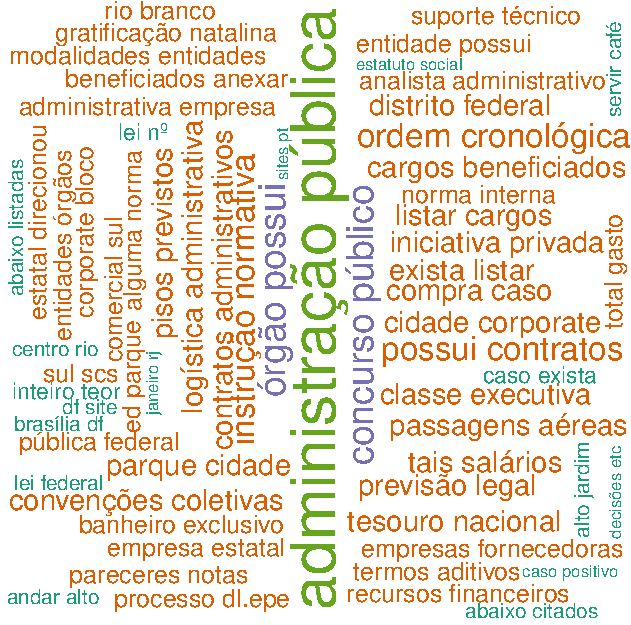
\includegraphics{markdown_v24_files/figure-latex/wordcloud_bigram_DIR02_semstopwords-1.pdf}

\begin{Shaded}
\begin{Highlighting}[]
\NormalTok{## DEA}
\CommentTok{#jpeg("XX_wordclou_tfidf_dir03_DEA.jpeg")}
\NormalTok{nuvem3.}\DecValTok{2}\NormalTok{ =}\StringTok{ }
\NormalTok{plot_diretorias_tf_dif_bigram2 }\OperatorTok
\StringTok{  }\KeywordTok{filter}\NormalTok{(DIRETORIA }\OperatorTok{==}\StringTok{ "DEA"}\NormalTok{) }\OperatorTok
\StringTok{  }\KeywordTok{select}\NormalTok{(}\OperatorTok{-}\NormalTok{DIRETORIA, }\DataTypeTok{word =}\NormalTok{ BIGRAM,}\DataTypeTok{freq =}\NormalTok{ tf_idf) }\OperatorTok
\StringTok{  }\CommentTok{#top_n(150, freq) %>%}
\StringTok{  }\KeywordTok{as.data.frame}\NormalTok{() }

\KeywordTok{set.seed}\NormalTok{(}\DecValTok{543453}\NormalTok{)}
\KeywordTok{wordcloud}\NormalTok{(}\DataTypeTok{words =}\NormalTok{ nuvem3.}\DecValTok{2}\OperatorTok{$}\NormalTok{word, }\DataTypeTok{freq =}\NormalTok{ nuvem3.}\DecValTok{2}\OperatorTok{$}\NormalTok{freq,}
          \DataTypeTok{max.words=}\DecValTok{250}\NormalTok{, }\DataTypeTok{random.order=}\OtherTok{FALSE}\NormalTok{, }\DataTypeTok{rot.per=}\FloatTok{0.35}\NormalTok{, }
          \DataTypeTok{colors=}\KeywordTok{brewer.pal}\NormalTok{(}\DecValTok{10}\NormalTok{, }\StringTok{"Dark2"}\NormalTok{))}
\end{Highlighting}
\end{Shaded}

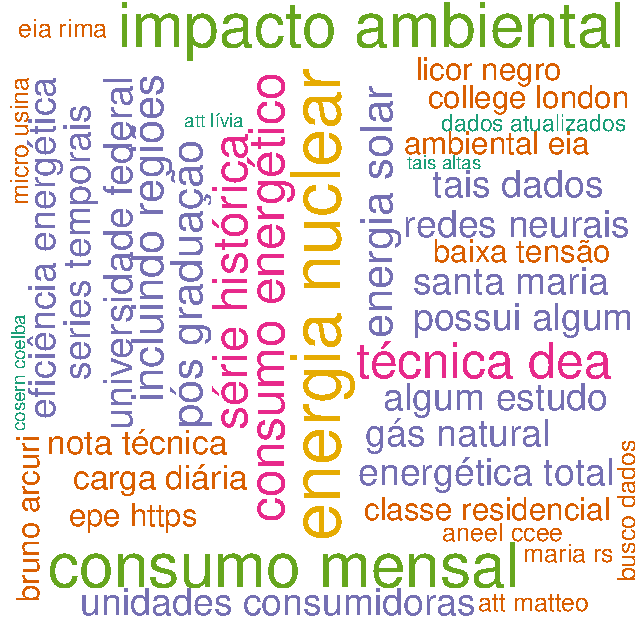
\includegraphics{markdown_v24_files/figure-latex/wordcloud_bigram_DIR03_semstopwords-1.pdf}

\begin{Shaded}
\begin{Highlighting}[]
\NormalTok{## DPG}
\CommentTok{#jpeg("XX_wordclou_tfidf_dir04_DPG.jpeg")}
\NormalTok{nuvem4.}\DecValTok{2}\NormalTok{ =}\StringTok{ }
\NormalTok{plot_diretorias_tf_dif_bigram2 }\OperatorTok
\StringTok{  }\KeywordTok{filter}\NormalTok{(DIRETORIA }\OperatorTok{==}\StringTok{ "DPG"}\NormalTok{) }\OperatorTok
\StringTok{  }\KeywordTok{select}\NormalTok{(}\OperatorTok{-}\NormalTok{DIRETORIA, }\DataTypeTok{word =}\NormalTok{ BIGRAM,}\DataTypeTok{freq =}\NormalTok{ tf_idf) }\OperatorTok
\StringTok{  }\CommentTok{#top_n(150, freq) %>%}
\StringTok{  }\KeywordTok{as.data.frame}\NormalTok{() }

\KeywordTok{set.seed}\NormalTok{(}\DecValTok{75437}\NormalTok{)}
\KeywordTok{wordcloud}\NormalTok{(}\DataTypeTok{words =}\NormalTok{ nuvem4.}\DecValTok{2}\OperatorTok{$}\NormalTok{word, }\DataTypeTok{freq =}\NormalTok{ nuvem4.}\DecValTok{2}\OperatorTok{$}\NormalTok{freq, }\DataTypeTok{min.freq =} \FloatTok{0.1}\NormalTok{,}
          \DataTypeTok{max.words=}\DecValTok{250}\NormalTok{, }\DataTypeTok{random.order=}\OtherTok{FALSE}\NormalTok{, }\DataTypeTok{rot.per=}\FloatTok{0.35}\NormalTok{, }
          \DataTypeTok{colors=}\KeywordTok{brewer.pal}\NormalTok{(}\DecValTok{10}\NormalTok{, }\StringTok{"Dark2"}\NormalTok{))}
\end{Highlighting}
\end{Shaded}

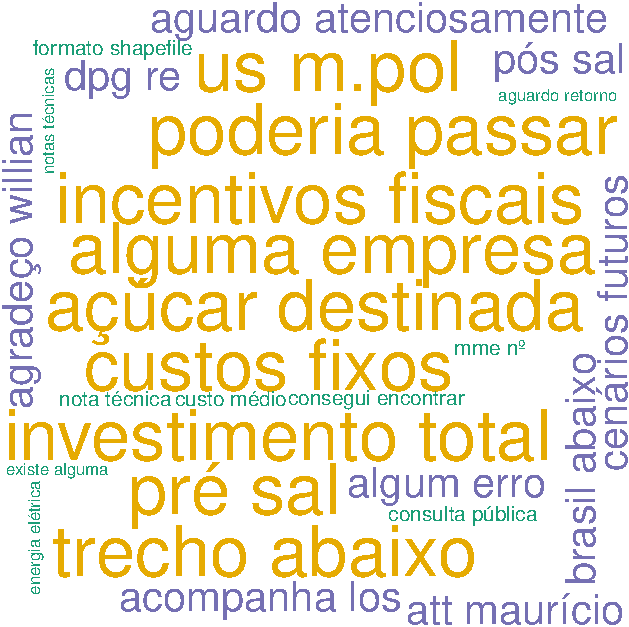
\includegraphics{markdown_v24_files/figure-latex/wordcloud_bigram_DIR04_semstopwords-1.pdf}

\begin{Shaded}
\begin{Highlighting}[]
\NormalTok{## OUTROS}
\CommentTok{#jpeg("XX_wordclou_tfidf_dir05_OUTROS.jpeg")}
\NormalTok{nuvem5.}\DecValTok{2}\NormalTok{ =}\StringTok{ }
\NormalTok{plot_diretorias_tf_dif_bigram2 }\OperatorTok
\StringTok{  }\KeywordTok{filter}\NormalTok{(DIRETORIA }\OperatorTok{==}\StringTok{ "OUTROS"}\NormalTok{) }\OperatorTok
\StringTok{  }\KeywordTok{select}\NormalTok{(}\OperatorTok{-}\NormalTok{DIRETORIA, }\DataTypeTok{word =}\NormalTok{ BIGRAM,}\DataTypeTok{freq =}\NormalTok{ tf_idf) }\OperatorTok
\StringTok{  }\CommentTok{#top_n(150, freq) %>%}
\StringTok{  }\KeywordTok{as.data.frame}\NormalTok{() }

\KeywordTok{set.seed}\NormalTok{(}\DecValTok{75437}\NormalTok{)}
\KeywordTok{wordcloud}\NormalTok{(}\DataTypeTok{words =}\NormalTok{ nuvem5.}\DecValTok{2}\OperatorTok{$}\NormalTok{word, }\DataTypeTok{freq =}\NormalTok{ nuvem5.}\DecValTok{2}\OperatorTok{$}\NormalTok{freq, }\DataTypeTok{min.freq =} \FloatTok{0.1}\NormalTok{,}
          \DataTypeTok{max.words=}\DecValTok{250}\NormalTok{, }\DataTypeTok{random.order=}\OtherTok{FALSE}\NormalTok{, }\DataTypeTok{rot.per=}\FloatTok{0.35}\NormalTok{, }
          \DataTypeTok{colors=}\KeywordTok{brewer.pal}\NormalTok{(}\DecValTok{10}\NormalTok{, }\StringTok{"Dark2"}\NormalTok{))}
\end{Highlighting}
\end{Shaded}

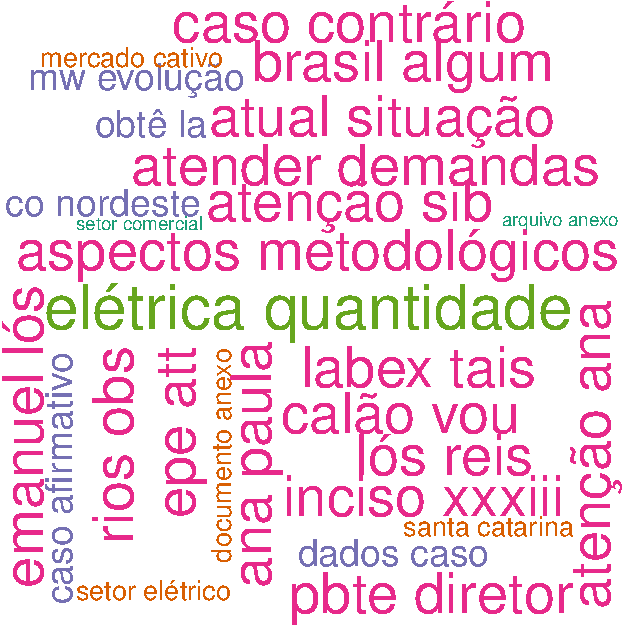
\includegraphics{markdown_v24_files/figure-latex/wordcloud_bigram_DIR05_semstopwords-1.pdf}

\begin{Shaded}
\begin{Highlighting}[]
\CommentTok{#View(head(plot_diretoria_palavras))}
\NormalTok{library(wordcloud2)}

\NormalTok{plot_diretorias_tf_dif_bigram2 = bigrams2 %>%}
\NormalTok{  select(BIGRAM,n,DIRETORIA) %>%}
\NormalTok{  bind_tf_idf(BIGRAM, DIRETORIA, n) %>%}
\NormalTok{  arrange(desc(tf_idf)) %>%}
\NormalTok{  mutate(BIGRAM = factor(BIGRAM, levels = rev(unique(BIGRAM)))) %>%}
\NormalTok{  mutate(DIRETORIA = factor(DIRETORIA,levels=c(}\StringTok{"DEA"}\NormalTok{,}\StringTok{"DEE"}\NormalTok{,}\StringTok{"DGC"}\NormalTok{,}\StringTok{"DPG"}\NormalTok{,}\StringTok{"OUTROS"}\NormalTok{))) %>%}
\NormalTok{  select(BIGRAM, tf_idf, DIRETORIA)}
  

\CommentTok{## DEE}
\CommentTok{#jpeg("XX_wordclou_tfidf_dir01_DEE.jpeg")}
\NormalTok{set.seed(233115)}
\NormalTok{plot_diretorias_tf_dif_bigram2 %>%}
\NormalTok{  filter(DIRETORIA == }\StringTok{"DEE"}\NormalTok{) %>%}
\NormalTok{  top_n(150, tf_idf) %>%}
\NormalTok{  wordcloud2(shuffle = TRUE, }
\NormalTok{             color = }\StringTok{"random-dark"}\NormalTok{,}
\NormalTok{             shape = }\StringTok{"circle"}\NormalTok{)}

\CommentTok{## DGC}
\CommentTok{#jpeg("XX_wordclou_tfidf_dir02_DGC.jpeg")}
\NormalTok{set.seed(233115)}
\NormalTok{plot_diretorias_tf_dif_bigram2 %>%}
\NormalTok{  filter(DIRETORIA == }\StringTok{"DGC"}\NormalTok{) %>%}
\NormalTok{  top_n(150, tf_idf) %>%}
\NormalTok{  wordcloud2()}

\CommentTok{## DEA}
\CommentTok{#jpeg("XX_wordclou_tfidf_dir03_DEA.jpeg")}
\NormalTok{set.seed(233115)}
\NormalTok{plot_diretorias_tf_dif_bigram2 %>%}
\NormalTok{  filter(DIRETORIA == }\StringTok{"DEA"}\NormalTok{) %>%}
\NormalTok{  top_n(150, tf_idf) %>%}
\NormalTok{  wordcloud2()}

\CommentTok{## DPG}
\CommentTok{#jpeg("XX_wordclou_tfidf_dir04_DPG.jpeg")}
\NormalTok{set.seed(233115)}
\NormalTok{plot_diretorias_tf_dif_bigram2 %>%}
\NormalTok{  filter(DIRETORIA == }\StringTok{"DPG"}\NormalTok{) %>%}
\NormalTok{  top_n(150, tf_idf) %>%}
\NormalTok{  wordcloud2()}

\CommentTok{## OUTROS}
\CommentTok{#jpeg("XX_wordclou_tfidf_dir05_OUTROS.jpeg")}
\NormalTok{set.seed(233115)}
\NormalTok{plot_diretorias_tf_dif_bigram2 %>%}
\NormalTok{  filter(DIRETORIA == }\StringTok{"OUTROS"}\NormalTok{) %>%}
\NormalTok{  top_n(150, tf_idf) %>%}
\NormalTok{  wordcloud2()}
\end{Highlighting}
\end{Shaded}

\paragraph{Gráfico da estatística tf\_idf c/ remoção de
stopwords}\label{grafico-da-estatistica-tf_idf-c-remocao-de-stopwords}

\begin{Shaded}
\begin{Highlighting}[]
\NormalTok{plot_diretorias_tf_dif_bigram2 }\OperatorTok
\KeywordTok{group_by}\NormalTok{(DIRETORIA) }\OperatorTok
\KeywordTok{top_n}\NormalTok{(}\DecValTok{10}\NormalTok{, tf_idf) }\OperatorTok
\KeywordTok{ungroup}\NormalTok{() }\OperatorTok
\KeywordTok{mutate}\NormalTok{(}\DataTypeTok{BIGRAM =} \KeywordTok{reorder}\NormalTok{(BIGRAM, tf_idf)) }\OperatorTok
\KeywordTok{ggplot}\NormalTok{(}\KeywordTok{aes}\NormalTok{(BIGRAM, tf_idf, }\DataTypeTok{fill =}\NormalTok{ DIRETORIA)) }\OperatorTok{+}
\KeywordTok{geom_col}\NormalTok{(}\DataTypeTok{show.legend =} \OtherTok{FALSE}\NormalTok{) }\OperatorTok{+}
\KeywordTok{labs}\NormalTok{(}\DataTypeTok{x =} \OtherTok{NULL}\NormalTok{, }\DataTypeTok{y =} \StringTok{"tf-idf"}\NormalTok{) }\OperatorTok{+}
\KeywordTok{facet_wrap}\NormalTok{(}\OperatorTok{~}\NormalTok{DIRETORIA, }\DataTypeTok{ncol =} \DecValTok{2}\NormalTok{, }\DataTypeTok{scales =} \StringTok{"free"}\NormalTok{) }\OperatorTok{+}
\KeywordTok{coord_flip}\NormalTok{() }\OperatorTok{+}\StringTok{ }
\KeywordTok{scale_y_continuous}\NormalTok{(}\DataTypeTok{labels=}\NormalTok{gcomma)}
\end{Highlighting}
\end{Shaded}

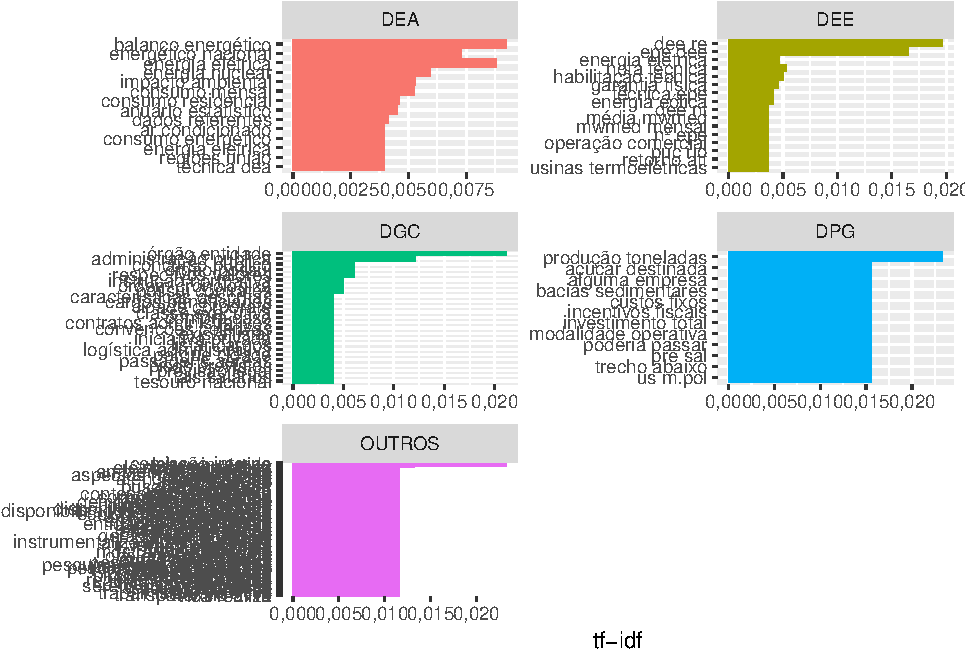
\includegraphics{markdown_v24_files/figure-latex/unnamed-chunk-48-1.pdf}

\paragraph{Nuvem de palavras por diretoria - s/ steeming e/ou stopwords
-
trigram}\label{nuvem-de-palavras-por-diretoria---s-steeming-eou-stopwords---trigram}

\begin{Shaded}
\begin{Highlighting}[]
\CommentTok{#View(head(plot_diretoria_palavras))}
\KeywordTok{library}\NormalTok{(wordcloud)}
\NormalTok{plot_diretorias_tf_dif_trigram =}\StringTok{ }\NormalTok{DB }\OperatorTok
\StringTok{  }\KeywordTok{select}\NormalTok{(DESCRI_PEDIDO,DIRETORIA) }\OperatorTok
\StringTok{  }\KeywordTok{unnest_tokens}\NormalTok{(TRIGRAM, DESCRI_PEDIDO, }\DataTypeTok{token =} \StringTok{"ngrams"}\NormalTok{, }\DataTypeTok{n =} \DecValTok{3}\NormalTok{) }\OperatorTok
\StringTok{  }\KeywordTok{count}\NormalTok{(DIRETORIA, TRIGRAM, }\DataTypeTok{sort =} \OtherTok{TRUE}\NormalTok{) }\OperatorTok
\StringTok{  }\KeywordTok{bind_tf_idf}\NormalTok{(TRIGRAM, DIRETORIA, n) }\OperatorTok
\StringTok{  }\KeywordTok{arrange}\NormalTok{(}\KeywordTok{desc}\NormalTok{(tf_idf)) }\OperatorTok
\StringTok{  }\KeywordTok{mutate}\NormalTok{(}\DataTypeTok{TRIGRAM =} \KeywordTok{factor}\NormalTok{(TRIGRAM, }\DataTypeTok{levels =} \KeywordTok{rev}\NormalTok{(}\KeywordTok{unique}\NormalTok{(TRIGRAM)))) }\OperatorTok
\StringTok{  }\KeywordTok{mutate}\NormalTok{(}\DataTypeTok{DIRETORIA =} \KeywordTok{factor}\NormalTok{(DIRETORIA,}\DataTypeTok{levels=}\KeywordTok{c}\NormalTok{(}\StringTok{"DEA"}\NormalTok{,}\StringTok{"DEE"}\NormalTok{,}\StringTok{"DGC"}\NormalTok{,}\StringTok{"DPG"}\NormalTok{,}\StringTok{"OUTROS"}\NormalTok{))) }\OperatorTok
\StringTok{  }\KeywordTok{select}\NormalTok{(TRIGRAM, tf_idf, DIRETORIA)}
\end{Highlighting}
\end{Shaded}

\begin{Shaded}
\begin{Highlighting}[]
\NormalTok{## DEE}
\CommentTok{#jpeg("wordcloud_tfidf_dir01_DEE_trigram_comstop_semstemming.jpeg")}
\NormalTok{nuvem1.}\DecValTok{3}\NormalTok{ =}\StringTok{ }
\NormalTok{plot_diretorias_tf_dif_trigram }\OperatorTok
\StringTok{  }\KeywordTok{filter}\NormalTok{(DIRETORIA }\OperatorTok{==}\StringTok{ "DEE"}\NormalTok{) }\OperatorTok
\StringTok{  }\KeywordTok{select}\NormalTok{(}\OperatorTok{-}\NormalTok{DIRETORIA, }\DataTypeTok{word =}\NormalTok{ TRIGRAM,}\DataTypeTok{freq =}\NormalTok{ tf_idf) }\OperatorTok
\StringTok{  }\CommentTok{#top_n(150, freq) %>%}
\StringTok{  }\KeywordTok{as.data.frame}\NormalTok{() }

\KeywordTok{set.seed}\NormalTok{(}\DecValTok{8835}\NormalTok{)}
\KeywordTok{wordcloud}\NormalTok{(}\DataTypeTok{words =}\NormalTok{ nuvem1.}\DecValTok{3}\OperatorTok{$}\NormalTok{word, }\DataTypeTok{freq =}\NormalTok{ nuvem1.}\DecValTok{3}\OperatorTok{$}\NormalTok{freq, }\DataTypeTok{min.freq =} \FloatTok{0.2}\NormalTok{,}
          \DataTypeTok{max.words=}\DecValTok{250}\NormalTok{, }\DataTypeTok{random.order=}\OtherTok{FALSE}\NormalTok{, }\DataTypeTok{rot.per=}\FloatTok{0.35}\NormalTok{, }
          \DataTypeTok{colors=}\KeywordTok{brewer.pal}\NormalTok{(}\DecValTok{10}\NormalTok{, }\StringTok{"Dark2"}\NormalTok{))}
\end{Highlighting}
\end{Shaded}

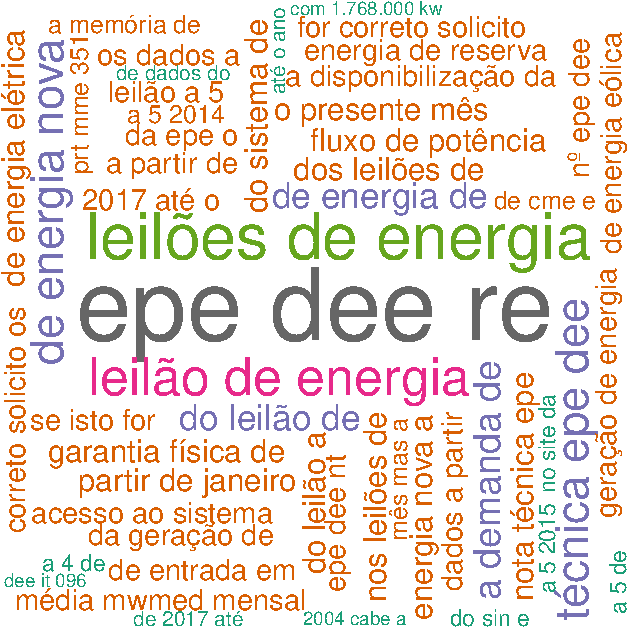
\includegraphics{markdown_v24_files/figure-latex/wordcloud_trigram_DIR01_comstopwords-1.pdf}

\begin{Shaded}
\begin{Highlighting}[]
\CommentTok{#dev.off()}
\end{Highlighting}
\end{Shaded}

\begin{Shaded}
\begin{Highlighting}[]
\NormalTok{## DGC}
\CommentTok{#jpeg("wordcloud_tfidf_dir02_DGC_trigram_comstop_semstemming.jpeg")}
\NormalTok{nuvem2.}\DecValTok{3}\NormalTok{ =}\StringTok{ }
\NormalTok{plot_diretorias_tf_dif_trigram }\OperatorTok
\StringTok{  }\KeywordTok{filter}\NormalTok{(DIRETORIA }\OperatorTok{==}\StringTok{ "DGC"}\NormalTok{) }\OperatorTok
\StringTok{  }\KeywordTok{select}\NormalTok{(}\OperatorTok{-}\NormalTok{DIRETORIA, }\DataTypeTok{word =}\NormalTok{ TRIGRAM,}\DataTypeTok{freq =}\NormalTok{ tf_idf) }\OperatorTok
\StringTok{  }\CommentTok{#top_n(150, freq) %>%}
\StringTok{  }\KeywordTok{as.data.frame}\NormalTok{() }

\KeywordTok{set.seed}\NormalTok{(}\DecValTok{1273}\NormalTok{)}
\KeywordTok{wordcloud}\NormalTok{(}\DataTypeTok{words =}\NormalTok{ nuvem2.}\DecValTok{3}\OperatorTok{$}\NormalTok{word, }\DataTypeTok{freq =}\NormalTok{ nuvem2.}\DecValTok{3}\OperatorTok{$}\NormalTok{freq, }\DataTypeTok{min.freq =} \FloatTok{0.2}\NormalTok{,}
          \DataTypeTok{max.words=}\DecValTok{250}\NormalTok{, }\DataTypeTok{random.order=}\OtherTok{FALSE}\NormalTok{, }\DataTypeTok{rot.per=}\FloatTok{0.35}\NormalTok{, }
          \DataTypeTok{colors=}\KeywordTok{brewer.pal}\NormalTok{(}\DecValTok{10}\NormalTok{, }\StringTok{"Dark2"}\NormalTok{))}
\end{Highlighting}
\end{Shaded}

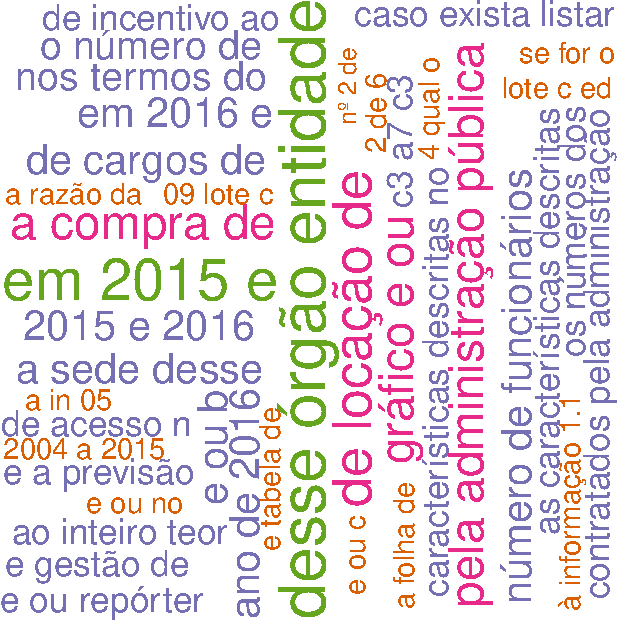
\includegraphics{markdown_v24_files/figure-latex/wordcloud_trigram_DIR02_comstopwords-1.pdf}

\begin{Shaded}
\begin{Highlighting}[]
\NormalTok{## DEA}
\CommentTok{#jpeg("XX_wordclou_tfidf_dir03_DEA_trigram_comstop_semstemming.jpeg")}
\NormalTok{nuvem3.}\DecValTok{3}\NormalTok{ =}\StringTok{ }
\NormalTok{plot_diretorias_tf_dif_trigram }\OperatorTok
\StringTok{  }\KeywordTok{filter}\NormalTok{(DIRETORIA }\OperatorTok{==}\StringTok{ "DEA"}\NormalTok{) }\OperatorTok
\StringTok{  }\KeywordTok{select}\NormalTok{(}\OperatorTok{-}\NormalTok{DIRETORIA, }\DataTypeTok{word =}\NormalTok{ TRIGRAM,}\DataTypeTok{freq =}\NormalTok{ tf_idf) }\OperatorTok
\StringTok{  }\CommentTok{#top_n(150, freq) %>%}
\StringTok{  }\KeywordTok{as.data.frame}\NormalTok{() }

\KeywordTok{set.seed}\NormalTok{(}\DecValTok{543453}\NormalTok{)}
\KeywordTok{wordcloud}\NormalTok{(}\DataTypeTok{words =}\NormalTok{ nuvem3.}\DecValTok{3}\OperatorTok{$}\NormalTok{word, }\DataTypeTok{freq =}\NormalTok{ nuvem3.}\DecValTok{3}\OperatorTok{$}\NormalTok{freq,}
          \DataTypeTok{max.words=}\DecValTok{250}\NormalTok{, }\DataTypeTok{random.order=}\OtherTok{FALSE}\NormalTok{, }\DataTypeTok{rot.per=}\FloatTok{0.35}\NormalTok{, }
          \DataTypeTok{colors=}\KeywordTok{brewer.pal}\NormalTok{(}\DecValTok{10}\NormalTok{, }\StringTok{"Dark2"}\NormalTok{))}
\end{Highlighting}
\end{Shaded}

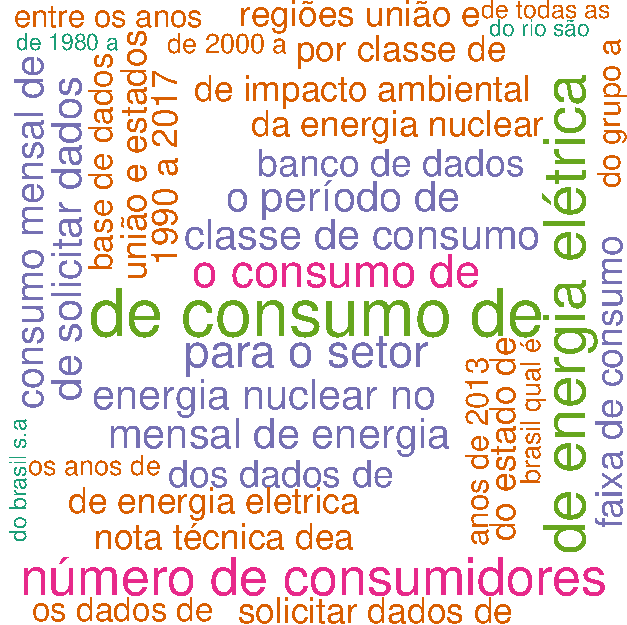
\includegraphics{markdown_v24_files/figure-latex/wordcloud_trigram_DIR03_comstopwords-1.pdf}

\begin{Shaded}
\begin{Highlighting}[]
\NormalTok{## DPG}
\CommentTok{#jpeg("XX_wordclou_tfidf_dir04_DPG_trigram_comstop_semstemming.jpeg")}
\NormalTok{nuvem4.}\DecValTok{3}\NormalTok{ =}\StringTok{ }
\NormalTok{plot_diretorias_tf_dif_trigram }\OperatorTok
\StringTok{  }\KeywordTok{filter}\NormalTok{(DIRETORIA }\OperatorTok{==}\StringTok{ "DPG"}\NormalTok{) }\OperatorTok
\StringTok{  }\KeywordTok{select}\NormalTok{(}\OperatorTok{-}\NormalTok{DIRETORIA, }\DataTypeTok{word =}\NormalTok{ TRIGRAM,}\DataTypeTok{freq =}\NormalTok{ tf_idf) }\OperatorTok
\StringTok{  }\CommentTok{#top_n(150, freq) %>%}
\StringTok{  }\KeywordTok{as.data.frame}\NormalTok{() }

\KeywordTok{set.seed}\NormalTok{(}\DecValTok{75437}\NormalTok{)}
\KeywordTok{wordcloud}\NormalTok{(}\DataTypeTok{words =}\NormalTok{ nuvem4.}\DecValTok{3}\OperatorTok{$}\NormalTok{word, }\DataTypeTok{freq =}\NormalTok{ nuvem4.}\DecValTok{3}\OperatorTok{$}\NormalTok{freq, }\DataTypeTok{min.freq =} \FloatTok{0.1}\NormalTok{,}
          \DataTypeTok{max.words=}\DecValTok{250}\NormalTok{, }\DataTypeTok{random.order=}\OtherTok{FALSE}\NormalTok{, }\DataTypeTok{rot.per=}\FloatTok{0.35}\NormalTok{, }
          \DataTypeTok{colors=}\KeywordTok{brewer.pal}\NormalTok{(}\DecValTok{10}\NormalTok{, }\StringTok{"Dark2"}\NormalTok{))}
\end{Highlighting}
\end{Shaded}

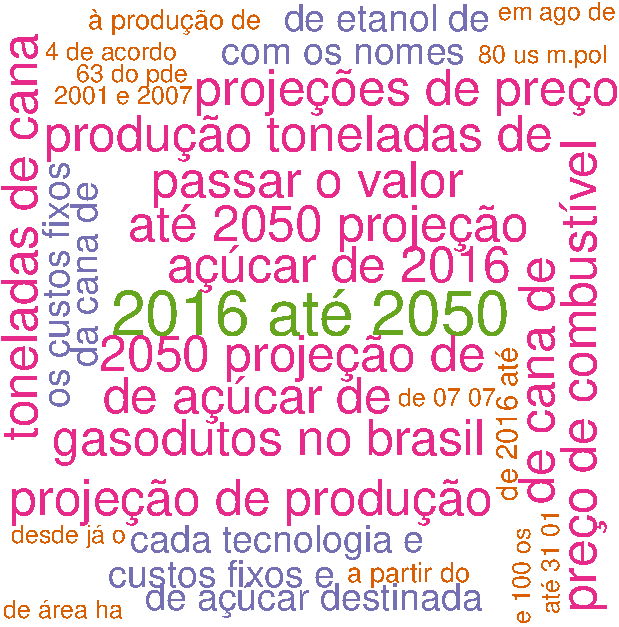
\includegraphics{markdown_v24_files/figure-latex/wordcloud_trigram_DIR04_comstopwords-1.pdf}

\begin{Shaded}
\begin{Highlighting}[]
\NormalTok{## OUTROS}
\CommentTok{#jpeg("XX_wordclou_tfidf_dir05_OUTROS_trigram_comstop_semstemming.jpeg")}
\NormalTok{nuvem5.}\DecValTok{3}\NormalTok{ =}\StringTok{ }
\NormalTok{plot_diretorias_tf_dif_trigram }\OperatorTok
\StringTok{  }\KeywordTok{filter}\NormalTok{(DIRETORIA }\OperatorTok{==}\StringTok{ "OUTROS"}\NormalTok{) }\OperatorTok
\StringTok{  }\KeywordTok{select}\NormalTok{(}\OperatorTok{-}\NormalTok{DIRETORIA, }\DataTypeTok{word =}\NormalTok{ TRIGRAM,}\DataTypeTok{freq =}\NormalTok{ tf_idf) }\OperatorTok
\StringTok{  }\CommentTok{#top_n(150, freq) %>%}
\StringTok{  }\KeywordTok{as.data.frame}\NormalTok{() }

\KeywordTok{set.seed}\NormalTok{(}\DecValTok{1235}\NormalTok{)}
\KeywordTok{wordcloud}\NormalTok{(}\DataTypeTok{words =}\NormalTok{ nuvem5.}\DecValTok{3}\OperatorTok{$}\NormalTok{word, }\DataTypeTok{freq =}\NormalTok{ nuvem5.}\DecValTok{3}\OperatorTok{$}\NormalTok{freq,}
          \DataTypeTok{max.words=}\DecValTok{100}\NormalTok{, }\DataTypeTok{random.order=}\OtherTok{FALSE}\NormalTok{, }\DataTypeTok{rot.per=}\FloatTok{0.35}\NormalTok{, }
          \DataTypeTok{colors=}\KeywordTok{brewer.pal}\NormalTok{(}\DecValTok{10}\NormalTok{, }\StringTok{"Dark2"}\NormalTok{))}
\end{Highlighting}
\end{Shaded}

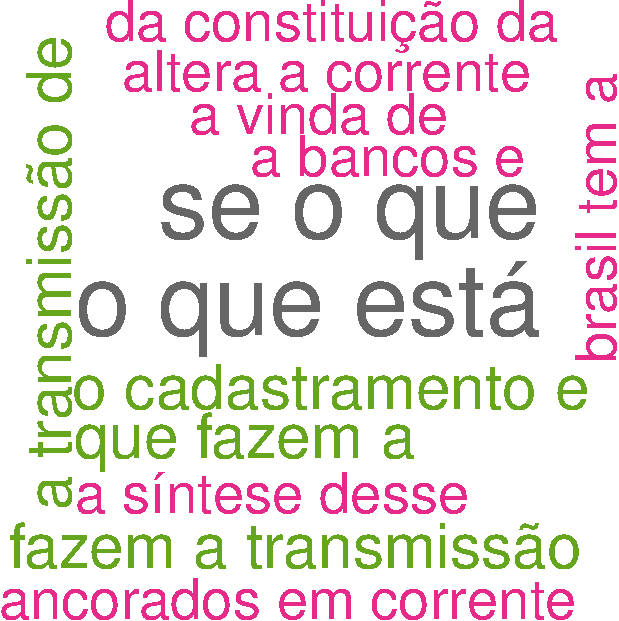
\includegraphics{markdown_v24_files/figure-latex/wordcloud_trigram_DIR05_comstopwords-1.pdf}

\begin{Shaded}
\begin{Highlighting}[]
\CommentTok{#View(head(plot_diretoria_palavras))}
\NormalTok{library(wordcloud2)}

\NormalTok{plot_diretorias_tf_dif_trigram = DB %>%}
\NormalTok{  select(DESCRI_PEDIDO,DIRETORIA) %>%}
\NormalTok{  unnest_tokens(TRIGRAM, DESCRI_PEDIDO, token = }\StringTok{"ngrams"}\NormalTok{, n = 3) %>%}
\NormalTok{  count(DIRETORIA, TRIGRAM, sort = TRUE) %>%}
\NormalTok{  bind_tf_idf(TRIGRAM, DIRETORIA, n) %>%}
\NormalTok{  arrange(desc(tf_idf)) %>%}
\NormalTok{  mutate(TRIGRAM = factor(TRIGRAM, levels = rev(unique(TRIGRAM)))) %>%}
\NormalTok{  mutate(DIRETORIA = factor(DIRETORIA,levels=c(}\StringTok{"DEA"}\NormalTok{,}\StringTok{"DEE"}\NormalTok{,}\StringTok{"DGC"}\NormalTok{,}\StringTok{"DPG"}\NormalTok{,}\StringTok{"OUTROS"}\NormalTok{))) %>%}
\NormalTok{  select(TRIGRAM, tf_idf, DIRETORIA)}
  

\CommentTok{## DEE}
\CommentTok{#jpeg("XX_wordclou_tfidf_dir01_DEE.jpeg")}
\NormalTok{set.seed(233115)}
\NormalTok{plot_diretorias_tf_dif_trigram %>%}
\NormalTok{  filter(DIRETORIA == }\StringTok{"DEE"}\NormalTok{) %>%}
\NormalTok{  top_n(150, tf_idf) %>%}
\NormalTok{  wordcloud2(shuffle = TRUE, }
\NormalTok{             color = }\StringTok{"random-dark"}\NormalTok{,}
\NormalTok{             shape = }\StringTok{"circle"}\NormalTok{)}

\CommentTok{## DGC}
\CommentTok{#jpeg("XX_wordclou_tfidf_dir02_DGC.jpeg")}
\NormalTok{set.seed(233115)}
\NormalTok{plot_diretorias_tf_dif_trigram %>%}
\NormalTok{  filter(DIRETORIA == }\StringTok{"DGC"}\NormalTok{) %>%}
\NormalTok{  top_n(150, tf_idf) %>%}
\NormalTok{  wordcloud2()}

\CommentTok{## DEA}
\CommentTok{#jpeg("XX_wordclou_tfidf_dir03_DEA.jpeg")}
\NormalTok{set.seed(233115)}
\NormalTok{plot_diretorias_tf_dif_trigram %>%}
\NormalTok{  filter(DIRETORIA == }\StringTok{"DEA"}\NormalTok{) %>%}
\NormalTok{  top_n(150, tf_idf) %>%}
\NormalTok{  wordcloud2()}

\CommentTok{## DPG}
\CommentTok{#jpeg("XX_wordclou_tfidf_dir04_DPG.jpeg")}
\NormalTok{set.seed(233115)}
\NormalTok{plot_diretorias_tf_dif_trigram %>%}
\NormalTok{  filter(DIRETORIA == }\StringTok{"DPG"}\NormalTok{) %>%}
\NormalTok{  top_n(150, tf_idf) %>%}
\NormalTok{  wordcloud2()}
  
\CommentTok{## OUTROS}
\CommentTok{#jpeg("XX_wordclou_tfidf_dir05_OUTROS.jpeg")}
\NormalTok{set.seed(233115)}
\NormalTok{plot_diretorias_tf_dif_trigram %>%}
\NormalTok{  filter(DIRETORIA == }\StringTok{"OUTROS"}\NormalTok{) %>%}
\NormalTok{  top_n(150, tf_idf) %>%}
\NormalTok{  wordcloud2()  }
\end{Highlighting}
\end{Shaded}


\end{document}
